\documentclass[letterpaper,11pt]{report}
\usepackage{float,captdef,multicol}
\usepackage{amssymb,amsmath,amsfonts,fancybox}
\usepackage[activeacute,spanish,es-tabla]{babel}
\usepackage[utf8]{inputenc}
\usepackage[colorlinks]{hyperref}
\usepackage{graphicx}
\usepackage{cancel}
\usepackage{marginnote}

\renewcommand*{\marginnotevadjust}{-0.1cm}
\renewcommand*{\marginfont}{\footnotesize}
\usepackage[right=4.5cm,left=2cm,top=3cm,bottom=3.0cm]{geometry}

%\usepackage[notref]{showkeys} % muestra los labels de las referencias.

\spanishdecimal{.}


\begin{document}

\sffamily

\thispagestyle{empty}
\begin{center}

\

\vspace{6.5cm}

\rule{15cm}{0.1cm}

\vspace{1.5cm}

{\huge \textsc{\textbf{ELECTRODIN'AMICA}}}

\vspace{1.5cm}

\rule{15cm}{0.1cm}

\vspace{1.5cm}

Versi'on del \today

\end{center}

\newpage
\thispagestyle{empty}
\ \\
\newpage
\setcounter{page}{1}
\pagenumbering{roman}

\pagestyle{plain}
\chapter*{Prefacio}
\addcontentsline{toc}{chapter}{Prefacio}
\bigskip
\bigskip
\bigskip
\bigskip
\bigskip
\bigskip


\emph{Este apunte ha sido escrito principalmente por \href{https://google.com/+GuillermoRubilar}{G. Rubilar} a partir de (e inspirado en) los cursos dictados por el Prof. Enrique Oelker en el \href{http://www.fisica.udec.cl/}{Departamento de F\'isica} de la \href{www.udec.cl}{Universidad de Concepci\'on}, y ha contado con las contribuciones de F. Izaurieta, E. Rodriguez, J. Saez, C. Salas, O. Jim'enez, F. Torres, P. Mella, J. Oliva, P. Utreras, J. Villegas, P. Mu\~noz, M.A. Sol'is y A. Maldonado.}

\bigskip


\bigskip

Esta obra ha sido publicada bajo una \href{https://github.com/gfrubi/electrodinamica/blob/master/LICENSE}{licencia GPL v3}. El c'odigo fuente (pdf)\LaTeX, as'i como las figuras en formato editable est'an disponibles en el \href{https://github.com/gfrubi/electrodinamica}{repositorio GitHub del proyecto}.
\bigskip
\bigskip
\bigskip

\fbox{Otros apuntes en \url{https://sites.google.com/site/apuntesdecienciasfisicas}.}

\bigskip
\bigskip
\bigskip



\emph{\textquotedblleft ...As\'i, nosotros los mortales, somos
inmortales en lo que creamos en com\'un."}

\begin{flushright}
Albert Einstein.
\end{flushright}

\newpage

\tableofcontents
\pagenumbering{arabic}
\setcounter{page}{1}

\chapter{Electrost'atica}
\pagenumbering{arabic}
\setcounter{page}{1}

\section{Introducci'on y conceptos fundamentales}

Uno de los conceptos fundamentales para la descripci'on de los
fen'omenos electromagn'eticos es el de \textit{carga el'ectrica}.
La carga el'ectrica es una propiedad f'isica de los cuerpos,
atribuida a ellos precisamente para diferenciar (o, en general,
describir) su comportamiento en las interacciones
electromagn'eticas. La experiencia ha mostrado que es posible
describir las propiedades de la interacci'on
electromagn'etica (por ejemplo, atracci'on, repulsi'on, o ausencia de fuerza) si
se asume que la magnitud f'isica llamada carga el'ectrica puede
adoptar valores positivos, negativos (o nulos), y que es una
propiedad aditiva (es decir, que la carga el'ectrica total de un
sistema formado por otras cargas es la suma algebraica de las
cargas constituyentes).

En general, la interacci'on electromagn'etica entre cargas puede ser bastante complicada. Por ejemplo, la fuerza que una carga ejerce sobre otra depende en general no s'olo de la distancia entre ellas, sino tambi'en de sus velocidades y aceleraciones relativas, y presenta adem'as efectos ``de retardo'' (esto quiere decir que la fuerza que una carga experimenta debido a la otra no depende de la posici'on, velocidad y aceleraci'on de la otra en el mismo instante, sino que en tiempos anteriores). Por esto, comenzaremos estudiando el caso m'as simple en que el sistema de cargas consideradas es \textit{estacionario}. En esta situaci'on los efectos de retardo y la dependencia con las velocidades y aceleraciones desaparecen, de modo que \textbf{las fuerzas electrost'aticas dependen s'olo de las distancias entre las cargas}.


\subsection{Ley de Coulomb}

En 1785 Coulomb\footnote{Charles Augustin de Coulomb: f'isico e ingeniero franc'es (1736-1806). Ver \url{http://es.wikipedia.org/wiki/Charles-Augustin_de_Coulomb}.} \textit{establece experimentalmente} que la fuerza entre dos cargas muy peque\~nas comparadas con la distancia que las separa (``puntuales'') es \textit{aproximadamente}  proporcional a la magnitud de las cargas, inversamente proporcional al cuadrado de la distancia entre ellas y en la direcci'on que las
une. Finalmente el sentido de la fuerza es tal que dos cargas de igual signo se repelen y dos de signos opuestos se atraen. Este resultado experimental, y por consiguiente necesariamente aproximado, es la base de la teor'ia de la interacci'on electrost'atica. Esta teor'ia \textit{asume} entonces que la fuerza entre cargas ``puntuales'' es \textit{exactamente} inversamente proporcional al cuadrado de la distancia que las separa y en la direcci'on de la l'inea que los une, de modo que
\begin{center}
\begin{figure}[H]
\centerline{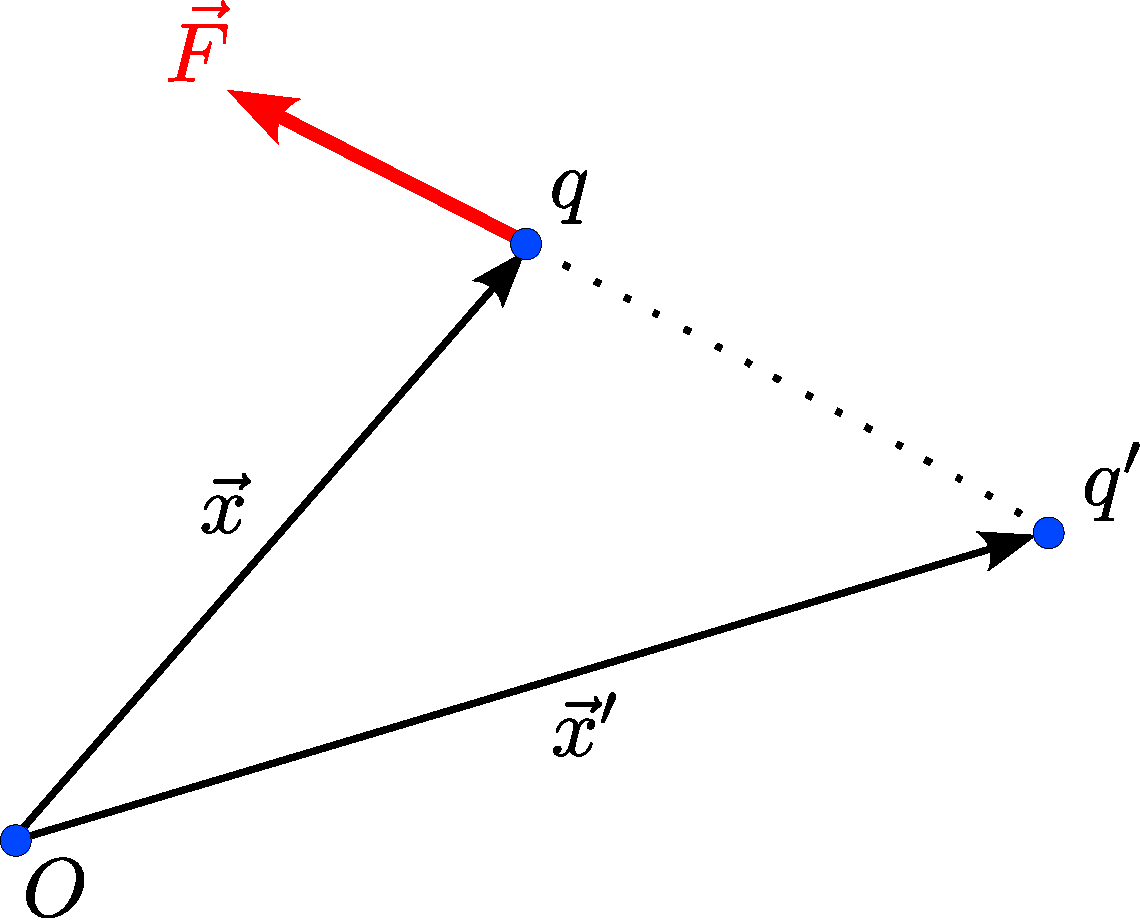
\psfig{file=fig/fig-Coulomb.pdf,height=4cm,angle=0}}
\caption{Fuerza electrost'atica entre dos cargas puntuales.}
\label{fig:Coulomb}
\end{figure}
\end{center}
\begin{equation}
F_i\propto \underbrace{\frac{qq'}{\left\vert \vec x-\vec
x'\right\vert^2}}_\text{magnitud}\cdot
\underbrace{\frac{x_i-x_i'}{\left\vert \vec x-\vec x'\right\vert }}_\text{vector unitario}.
\end{equation}
Podemos por tanto escribir
\begin{equation}
F_i=k\frac{qq'}{\left\vert \vec x-\vec x'\right\vert^2}
\cdot\frac{x_i-x_i'}{\left\vert \vec x-\vec x'\right\vert }.
\end{equation}
El valor de la constante $k$ depende del sistema de unidades usado para medir
magnitud de las cargas el'ectricas. Nosotros utilizaremos el sistema internacional SI (MKSA) donde la constante $k$ es denotada como\footnote{En el \textit{sistema gaussiano de unidades} (cgs) se
define $k:=1$ de modo que la unidad de carga no es independiente:
$[q]\stackrel{\text{cgs}}{=}cm^{3/2}g^{1/2}s^{-1}$. Esta unidad es llamada una
\textit{unidad electrost'atica} (esu) o un \textit{statCoulomb}.}%
\begin{equation}
k:=\frac{1}{4\pi\varepsilon_0},
\end{equation}
y donde $\varepsilon_0$ se conoce como la \textit{permitividad del vac\'{\i}o}, y
entonces
\begin{equation}\marginnote{Ley de Coulomb}
\boxed{F_i=\frac{qq'}{4\pi\varepsilon_0}\frac{\left(  x_i-x_i^{\prime
}\right)  }{\left\vert \vec x-\vec x'\right\vert ^3}.}\label{leycoulomb}%
\end{equation}
En el sistema SI, la constante
$k$ tiene el valor
\begin{equation}
k=c^2\times 10^{-7}\ Nm^2C^{-2},
\end{equation}
en que $c$ es la \textit{velocidad de la luz en el vac\'{\i}o}. Su valor es
$c=2.99792458\times 10^{8}\,ms^{-1}$. Con esto $k\approx 9.0\times
10^{9}\,Nm^2C^{-2}$, $\varepsilon _0\approx 8.854\times 10^{-12}
\,C^2N^{-1}m^{-2}$.

La expresi'on \eqref{leycoulomb} es conocida como \textit{ley de Coulomb}.
Adicionalmente, se \textit{asume} que la fuerza que ejerce un conjunto de $N$
cargas puntuales $q^{(\alpha)}$, $\alpha=1,\cdots N$, en posiciones $x^{(\alpha)}_i$ sobre una carga $q$ con posici'on $x_i$ es
\begin{equation}
F_i   =\sum_{\alpha=1}^{N}\frac{qq^{(\alpha)}}{4\pi\varepsilon_0}\frac{\left(
x_i-x^{(\alpha)}_i\right)  }{\left\vert  \vec x-\vec x^{(\alpha)}\right\vert^3}
=\frac{q}{4\pi\varepsilon_0}\sum_{\alpha=1}^{N}q^{(\alpha)}\frac{\left(
x_i-x^{(\alpha)}_i\right) }{\left\vert  \vec x-\vec
x^{(\alpha)}\right\vert^3}.\label{leycoulomb-discre}
\end{equation}
La suposici'on que esta fuerza sea la suma (vectorial) de las fuerzas individuales que
actuar'ia sobre la carga $q$ debido a cada una de las cargas $q^{(\alpha)}$ es
llamado \textit{principio de superposici'on}. Note que, como su nombre lo indica, este es un \textit{principio} en el que se basa la teor'ia electromagn'etica, ya que no es \textit{necesario a priori} que la interacci'on electrost'atica respete esta propiedad. En otras palabras, podr'ia ocurrir (o haber ocurrido) que la fuerza que dos cargas ejercen sobre una tercera no fuese \textit{exactamente} la suma vectorial de las fuerzas que cada una de ellas ejerce individualmente. Por ejemplo, hoy sabemos que esto 'ultimo es lo que efectivamente ocurre con la interacci'on gravitacional (!`\textit{no} satisface el principio de superposici'on!). En la teor'ia electromagn'etica se asume que la superposici'on es satisfecha en forma exacta. Como veremos, una consecuencia de este principio es que las ecuaciones que relacionan los campos el'ectricos (y sus respectivas fuerzas) con las distribuciones de carga que las producen est'an descritas por \textit{ecuaciones} (diferenciales y/o integrales) \textit{lineales}.


Para una \textit{distribuci'on continua de cargas} podemos considerar un elemento de
volumen $dV'$ conteniendo una carga $dq'=\rho(x')dV'$, donde $\rho(x')$ es
la densidad (volum'etrica) de carga (carga por unidad de volumen). Usando el
principio de superposici'on podemos escribir la fuerza total que esta
distribuci'on ejerce sobre una carga (puntual) de prueba $q$ como
\begin{align}
F_i  &= \int_V dF_i \\
& =\int_V\frac{q}{4\pi\varepsilon_0}\frac{\left(  x_i-x_i^{\prime
}\right)  }{\left\vert \vec x-\vec x'\right\vert ^3}dq^{\prime},
\end{align}
es decir,
\begin{equation}\marginnote{Fza. sobre carga puntual}
F_i  =\frac{q}{4\pi\varepsilon_0}\int_V\rho(x')\frac{\left(x_i-x_i'\right)
}{\left\vert \vec x-\vec x'\right\vert
^3}dV' .\label{leycoulomb-conti}
\end{equation}
An'alogamente, podemos describir cargas distribuidas en (regiones que puedan
aproximarse por) una superficie y/o curva usando la \textit{densidad superficial de
carga} $\sigma(x')$ (carga por unidad de 'area) y/o la \textit{densidad lineal de carga} $\lambda(x')$ (carga por unidad de longitud), de modo que $dq'=\sigma(x')dS$
y $dq'=\lambda(x')d\ell$, respectivamente.

\subsection{Campo el'ectrico}
El campo el'ectrico $E_i(\vec{x})$ en un punto $x_i$ es definido operacionalmente como la fuerza por unidad de carga \textit{sobre una carga muy peque\~na en tama\~no y magnitud} (``carga de prueba puntual'') $q$ situada en la posici'on $x_i$, es decir,
\begin{equation}
E_i(\vec x):=\lim_{q\rightarrow0}\frac{F_i}{q}.
\end{equation}
Note que el proceso l'imite ${q\rightarrow0}$ es necesario puesto que el uso de una carga $q$ de forma y magnitud arbitraria en general (mediante la fuerza de Coulomb) \textit{modificar'a la distribuci'on de cargas original}. Si la carga $q$ es cada vez m'as peque\~na en extensi'on y magnitud, entonces 'esta modificar'a cada vez menos la distribuci'on de carga original. En el l'imite ${q\rightarrow0}$, que ciertamente es una abstracci'on ya que en la pr'actica no existen cargas puntuales, ni tampoco cargas de magnitud arbitrariamente peque\~na, el cuociente $F_i/q$ ser'a independiente de la carga de prueba usada, y describir'a por lo tanto una cantidad dependiente s'olo de la distribuci'on de cargas considerada. Esto permite entonces considerar al campo el'ectrico como el campo \textit{generado por la distribuci'on de cargas}.

Con estas consideraciones, tenemos entonces que el campo el'ectrico generado por un conjunto de cargas puntuales $q^{(\alpha)}$ es dado por
\begin{equation}\marginnote{C. el'ectrico, cargas puntuales}
E_i(\vec x)=\frac{1}{4\pi\varepsilon_0}\sum_{\alpha=1
}^{N}q^{(\alpha)}\frac{\left(  x_i-x^{(\alpha)}_i\right)  }{\left\vert
\vec x-\vec x^{(\alpha)}\right\vert ^3}.\label{campelectr}
\end{equation}
Similarmente, para una distribuci'on volum'etrica de cargas:
\begin{equation}\marginnote{C. el'ectrico, distribuci'on}
\boxed{E_i(\vec x)=\frac{1}{4\pi\varepsilon_0}\int_V\rho(x')\frac{\left(
x_i-x_i'\right)  }{\left\vert \vec x-\vec x'\right\vert
^3}dV'.} \label{cerho}
\end{equation}
En general, preferiremos la descripci'on de la distribuci'on de cargas en t'erminos de la densidad volum'etrica $\rho(\vec{x})$, ya que a partir de ella podemos recobrar r'apidamente los otros casos de inter'es. Por ejemplo, podemos recobrar el resultado para el conjunto de cargas puntuales \eqref{campelectr} a partir de 
\eqref{cerho} si consideramos
\begin{equation}
\rho(\vec x)=\sum_{\alpha=1}^{N}q^{(\alpha)}\delta^{(3)}\left(\vec x-\vec
x^{(\alpha)}\right).
\label{conti-discre}
\end{equation}

\subsection{L'ineas de campo el'ectrico}
En electrodin'amica es 'util introducir el concepto de \textit{l'ineas de campo}. En el caso electrost'atico, asociado a cada configuraci'on de campo el'ectrico, descrito por el campo $E_i(\vec{x})$, es posible definir l'ineas de campo el'ectrico. Cada una de estas curvas, puede modelarse usando una parametrizaci'on de la forma $x_i=x_i(\lambda)$, donde $\lambda$ es un par'ametro real. Las l'ineas de campo son definidas como aquellas tales que sus vectores tangentes en cada punto son paralelos al vector campo el'ectrico. Esto es equivalente a la condici'on,
\begin{equation}\marginnote{L'ineas de campo}
\frac{dx_i}{d\lambda}(\lambda)=E_i(\vec{x}(\lambda)). \label{dlc}
\end{equation}
Note que, en general, es posible considerar un factor adicional al lado derecho de esta expresi'on (por ejemplo, $\alpha(\lambda)E_i(\vec{x}(\lambda))$ en lugar de $E_i(\vec{x}(\lambda))$), sin embargo la funci'on $\alpha(\lambda)$ puede siempre ser ``normalizada'' al valor $1$ redefiniendo convenientemente el par'ametro para describir la curva.

M'as expl'icitamente, la condici'on (\ref{dlc}) adopta, en coordenadas cartesianas y en tres dimensiones, la forma 
\begin{align}
\frac{dx}{d\lambda}(\lambda) &= {E_x}(x(\lambda),y(\lambda),z(\lambda)), \\
\frac{dy}{d\lambda}(\lambda) &= {E_y}(x(\lambda),y(\lambda),z(\lambda)),\\
\frac{dz}{d\lambda}(\lambda) &= \vec{E_z}(x(\lambda),y(\lambda),z(\lambda)),
\end{align}
de modo que define, dadas las componentes del campo $E_x(x,y,z)$, $E_y(x,y,z)$ y $E_y(x,y,z)$, un sistema de 3 ecuaciones diferenciales ordinarias acopladas, de primer orden, para las inc'ognitas $x(\lambda),y(\lambda)$ y $z(\lambda)$.

Una l'inea de campo particular queda determinada por la soluci'on del sistema de ecuaciones que satisface una determinada condici'on inicial, por ejemplo $\vec{x}(0)=\vec{x}_0$, donde $\vec{x}_0$ es un punto dado del espacio. La correspondiente soluci'on $\vec{x}(\lambda;\vec{x}_0)$ describir'a la l'inea de campo que pasa por el punto $\vec{x}_0$. Para algunos ejemplos, ver la figura\footnote{Figuras generadas usando VectorFieldPlot \cite{VFP}.} \ref{fig-E}.

\begin{center}
\begin{figure}[H]
\centerline{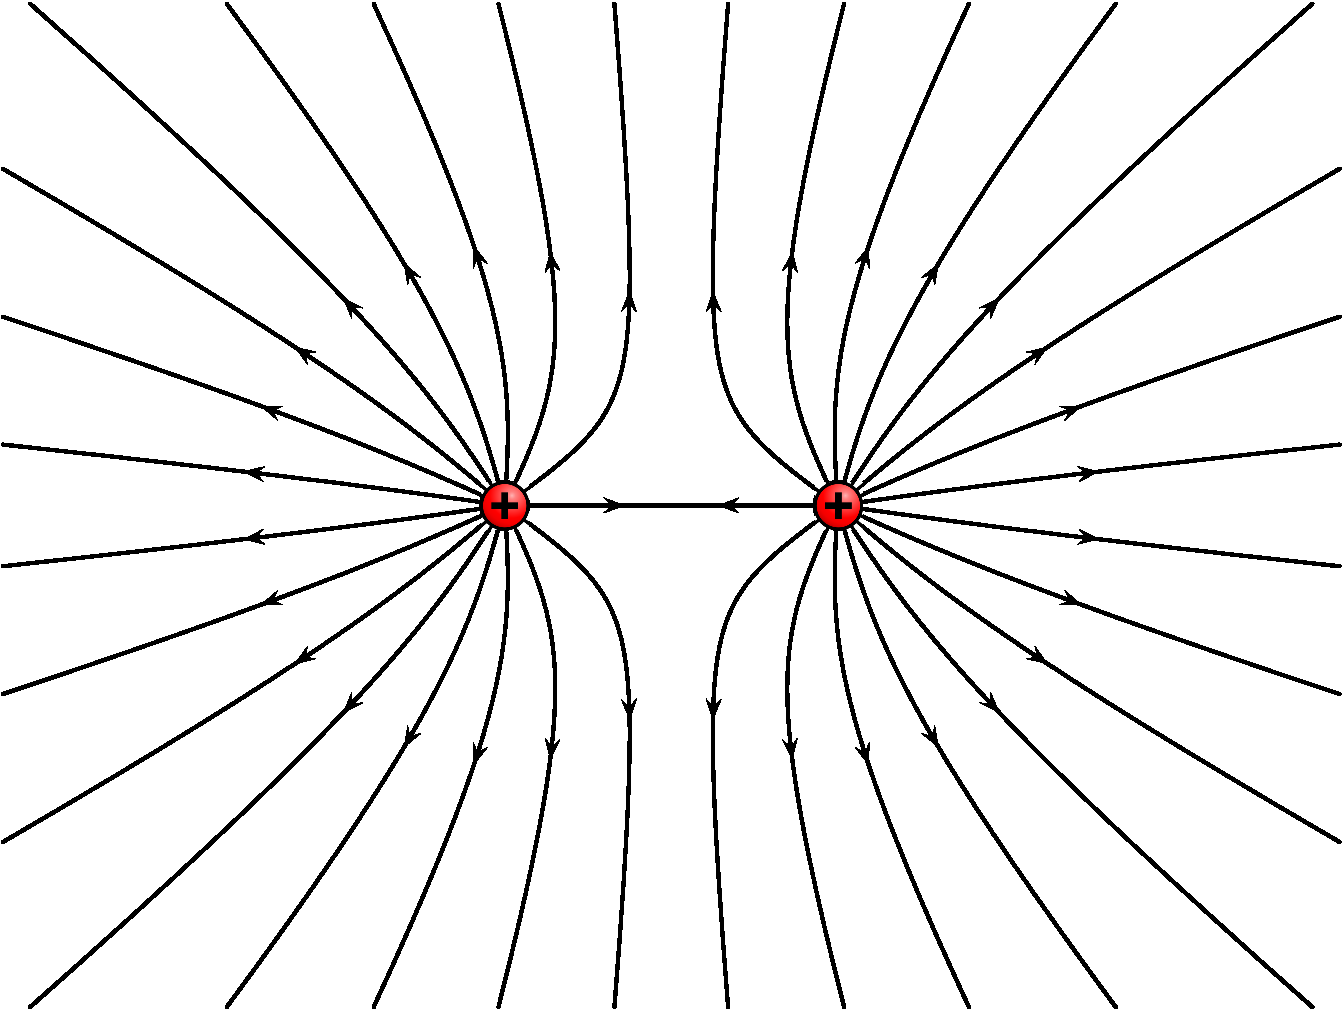
\psfig{file=fig/fig-E-01.pdf,height=4cm,angle=0}\hfill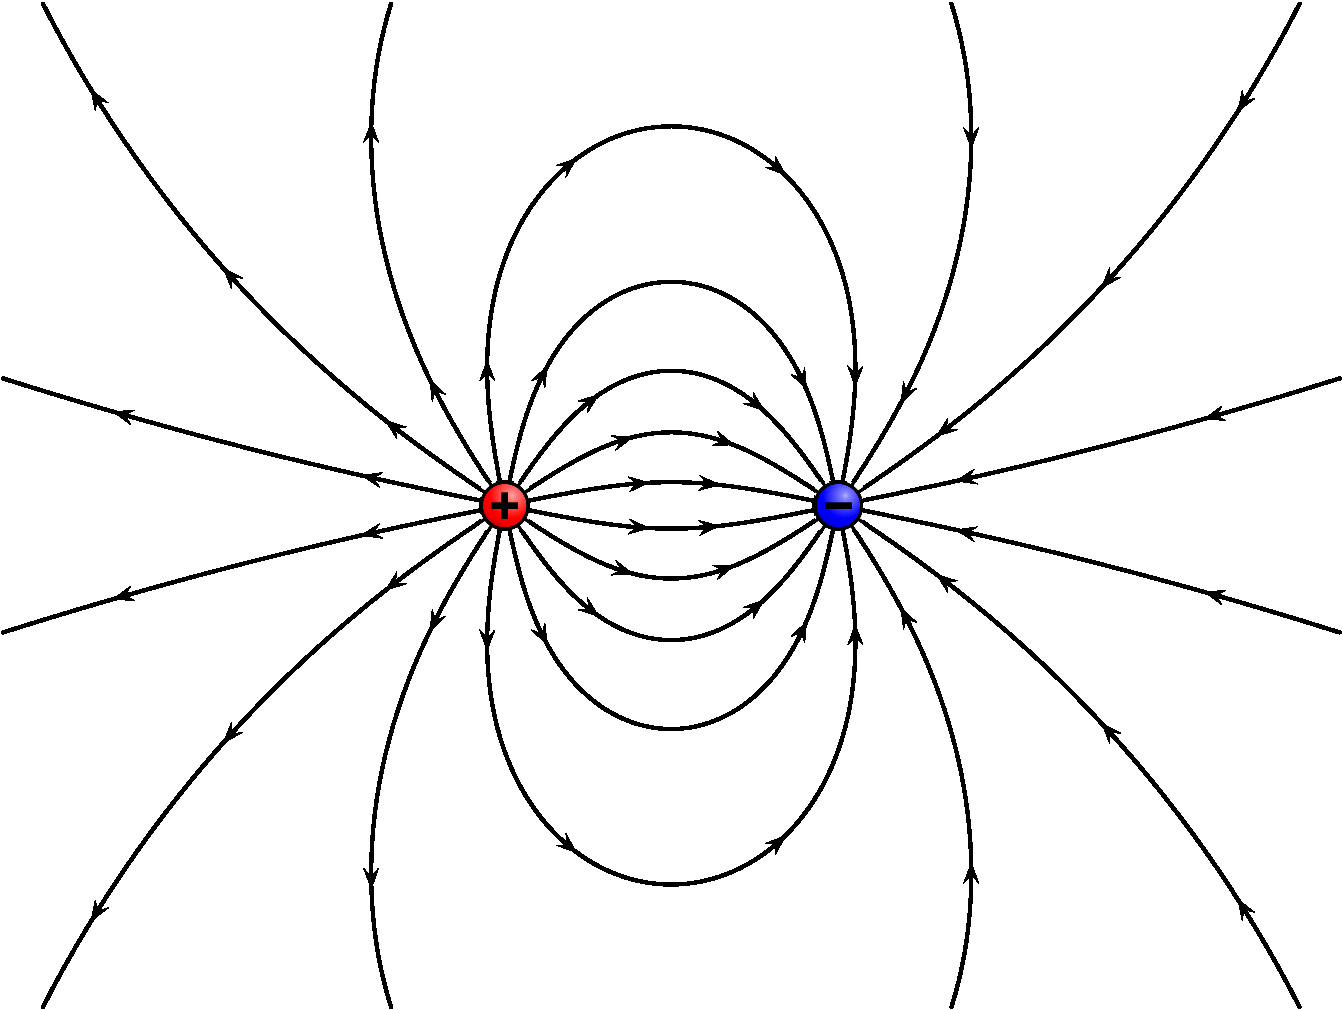
\psfig{file=fig/fig-E-02.pdf,height=4cm,angle=0}\hfill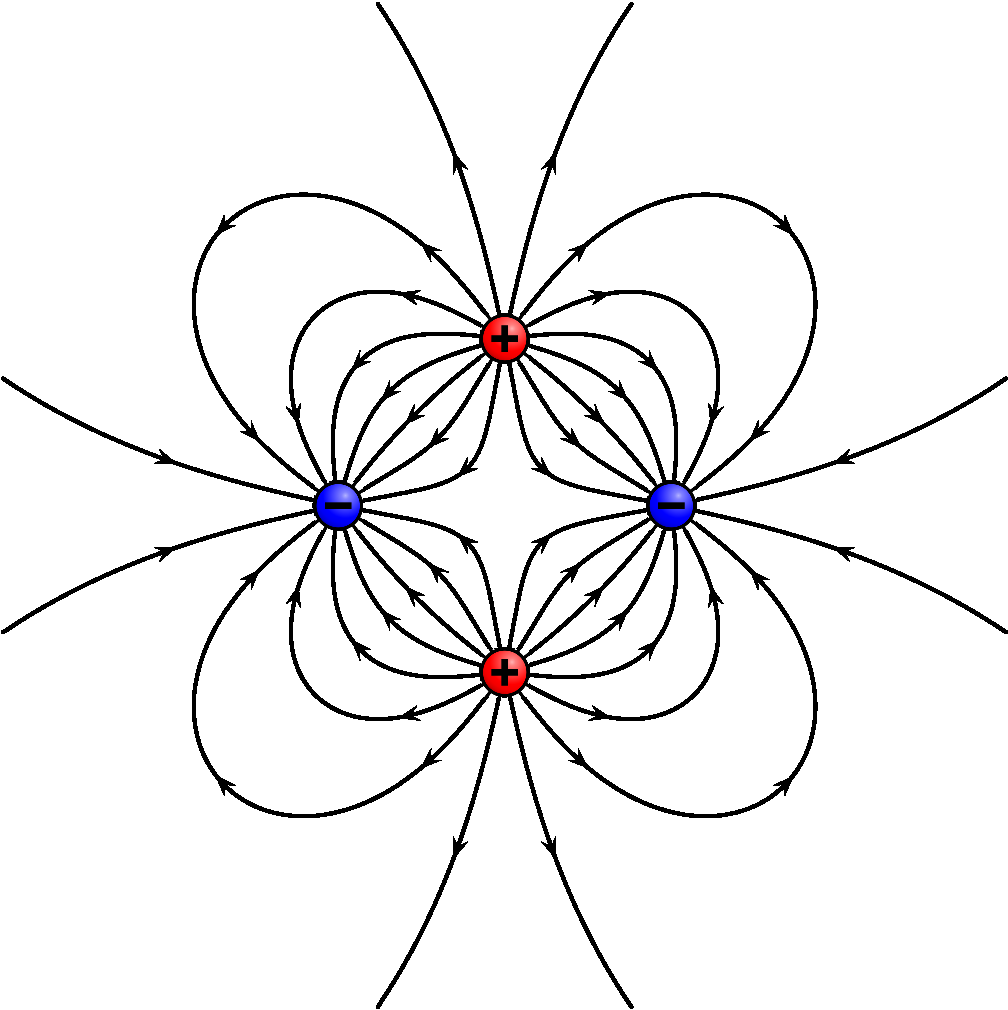
\psfig{file=fig/fig-E-03.pdf,height=4cm,angle=0}}
\caption{Ejemplos simples de l'ineas de campo el'ectrico.}
\label{fig-E}
\end{figure}
\end{center}
\subsection{Potencial el'ectrico}
Usando el hecho que
\begin{equation}
\frac{x_i-x_i'}{\left\vert \vec x-\vec x'\right\vert ^3}\equiv
-\partial_i\left( \frac{1}{\left\vert \vec x-\vec x'\right\vert
}\right), \label{id01}
\end{equation}
podemos escribir (\ref{cerho}) como
\begin{align}
E_i  & =\frac{1}{4\pi\varepsilon_0}\int_V\rho(x')\frac{\left(x_i-x_i'\right)
}{\left\vert \vec x-\vec x'\right\vert^3} dV' \\
&
=-\frac{1}{4\pi\varepsilon_0}\int_V\rho(x')\partial_i\left(\frac{1}{\left\vert
\vec x-\vec x'\right\vert }\right)  dV' \label{ein}\\
& =-\partial_i\left[\frac{1}{4\pi\varepsilon_0}\int_V\frac{\rho
(x')}{\left\vert \vec x-\vec x'\right\vert }dV'\right] \\
& =-\partial_i\phi ,
\end{align}
es decir,
\begin{equation}\marginnote{Campo a partir de potencial}
\boxed{\vec{E}(x)=-\vec\nabla\phi (x),} \label{E=nablaphi}
\end{equation}
donde hemos definido el \textit{potencial el'ectrico}
\begin{equation}\marginnote{Potencial electrost'atico}
\boxed{\phi(\vec x):=\frac{1}{4\pi\varepsilon_0}\int_V\frac{\rho(\vec x')}{
\left\vert \vec x-\vec x'\right\vert }dV' +\text{constante}.}\label{perho}
\end{equation}
Note que es posible agregar una constante arbitraria a la definici'on del
potencial. Por otro lado, es directo verificar que, como consecuencia directa de
(\ref{E=nablaphi}), todo campo el'ectrost'atico es irrotacional, es decir, su
rotor es nulo:
\begin{equation}\marginnote{C. el'ectrico irrotacional}
\boxed{\vec\nabla\times\vec{E}=\vec{0}.} \label{rotE0}
\end{equation}
Usando (\ref{E=nablaphi}), podemos expresar el potencial electrost'atico como
una integral de l'inea del campo el'ectrico:
\begin{equation}\marginnote{Potencial a partir de campo}
 \boxed{\phi(\vec{x})=\phi(\vec{x}_0)-\int_{\vec{x}_0}^{\vec{x}} \vec{E}\cdot
d\vec{x}.} \label{phiintE}
\end{equation}
Debido a (\ref{rotE0}) la integral (\ref{phiintE}) es independiente de la
trayectoria que une los puntes $\vec{x}_0$ y $\vec{x}$, o equivalentemente,
\begin{equation}\marginnote{C. el'ectrico sin circulaci'on}
 \boxed{\oint_{\cal C}\vec{E}\cdot d\vec{x}=0,} \label{ointE0}
\end{equation}
para toda curva cerrada $\cal C$. Note adem'as que de esta propiedad se desprende que las l'ineas de campo electrost'atico no pueden ser cerradas. En efecto, si existiese una l'inea de campo el'ectrico cerrada ${\cal C}$, entonces podemos evaluar $\oint_{\cal C}\vec{E}\cdot d\vec{x}$ sobre esta curva. Pero sobre una l'inea de campo se satisface que (\ref{dlc}), de modo que
\begin{align}
\oint_{\cal C}\vec{E}\cdot d\vec{x} &= \oint_{\cal C}\frac{d\vec{x}}{d\lambda}\cdot d\vec{x} \\
&= \oint_{\cal C}\frac{d\vec{x}}{d\lambda}\cdot \frac{d\vec{x}}{d\lambda}\,d\lambda \\
&= \oint_{\cal C}\left|\frac{d\vec{x}}{d\lambda}\right|^2 d\lambda \\
&>0 ,
\end{align}
en contradicci'on con (\ref{ointE0}).

Note que como consecuencia de (\ref{E=nablaphi}) o, equivalentemente, de (\ref{phiintE}) el vector campo el'ectrico es siempre \textit{normal a las superficies equipotenciales} (definidas como aquellos puntos que satisfacen $\phi(\vec{x})=\text{cte.}$) y su \textit{sentido es siempre hacia regiones de menor potencial}.

\section{Ley de Gauss}
Usando (\ref{ein}) podemos calcular la divergencia del campo el'ectrico:
\begin{eqnarray}
\partial_iE_i &=&-\partial_i\left[
\frac{1}{4\pi\varepsilon_0}\int_V\rho(x')\partial_i\left(\frac{1}{\left\vert
\vec x-\vec x'\right\vert }\right)  dV'\right] \\
&=&-
\frac{1}{4\pi\varepsilon_0}\int_V\rho(x')\partial_i\partial_i\left(\frac{1}{
\left\vert \vec x-\vec x'\right\vert }\right)  dV' \\
&=&-
\frac{1}{4\pi\varepsilon_0}\int_V\rho(x')\nabla^2\left(\frac{1}{\left\vert
\vec x-\vec x'\right\vert }\right)  dV' \\
&=&-
\frac{1}{4\pi\varepsilon_0}\int_V\rho(x')\left[-4\pi\delta^{(3)}(x_i-x_i')\right]
dV' \\
&=& \frac{1}{\varepsilon_0}\int_V\rho(x')\delta^{(3)}(x_i-x_i')\, dV' \\
&=& \frac{1}{\varepsilon_0}\rho(x).
\end{eqnarray}
Obtenemos as'i la \textbf{forma diferencial de la ley de Gauss}\footnote{Carl Friedrich Gauss, (1777-1855): matem'atico, astr'onomo y f'isico alem'an, ver \url{http://es.wikipedia.org/wiki/Carl_Friedrich_Gauss}.}:
\begin{equation}\marginnote{Ley de Gauss diferencial}
\boxed{\partial_iE_i =\frac{1}{\varepsilon_0}\rho(x).} \label{leygauss-dif}
\end{equation}
Usando el teorema de la divergencia (de Gauss!) para un volumen $V$ arbitrario
con borde $S=\partial V$, obtenemos
\begin{eqnarray}
\int_V\partial_iE_i\,dV'  &=&\frac{1}{\varepsilon_0}\int_V\rho(x')dV' ,\\
\oint_S E_idS_i &=&\frac{1}{\varepsilon_0}q_V,
\end{eqnarray}
donde $q_V$ es la carga neta en el volumen $V$. En notaci'on vectorial:
\begin{equation}\marginnote{Ley de Gauss integral}
\boxed{\oint_S \vec{E}\cdot d\vec{S} =\frac{1}{\varepsilon_0}q_V .}
\end{equation}
Esta es la \textbf{forma integral de la ley de Gauss}. Es importante recordar que la ley de Gauss en su forma integral es v'alida \textit{para todo volumen} $V$ y su correspondiente superficie ``gaussiana"\, $\partial V$. Debido a esta propiedad, la forma integral de la ley de Gauss resulta particularmente eficiente para determinar campos el'ectricos en situaciones altamente sim'etricas, donde es posible elegir el volumen de modo que $\vec{E}$ sea \textit{constante} sobre $\partial V$ (o al menos, sobre partes de $\partial V$).

\subsection{Ejemplo}
Plano infinito de densidad de carga constante
\begin{equation}
\vec{E}(x)=\left\{\begin{array}{rl}\frac{\sigma}{2\varepsilon_0}\hat{x},& x>0 \\
-\frac{\sigma}{2\varepsilon_0}\hat{x},& x<0 \end{array}\right. .
\end{equation}

\subsection{Ecuaci'on de Poisson y Laplace}
Usando (\ref{E=nablaphi}) y (\ref{leygauss-dif}) obtenemos
\begin{equation}
\partial_iE_i  =-\partial_i\partial_i\phi=\frac{\rho}{\varepsilon_0},
\end{equation}
es decir, el potencial el'ectrico satisface la \textbf{ecuaci'on de
Poisson}\footnote{Siméon Denis Poisson (1781-1840): matem'atico franc'es, ver \url{http://es.wikipedia.org/wiki/Sim\%C3\%A9on_Denis_Poisson}.}:
\begin{equation}\marginnote{Ec. de Poisson}
\boxed{\nabla^2\phi=-\frac{\rho}{\varepsilon_0}.}\label{poisson}
\end{equation}
Como consecuencia, el potencial electrost'atico en una regi'on libre de cargas
satisface la \textbf{ecuaci'on de Laplace}\footnote{Pierre Simon Laplace (1749-1827): matem'atico, f'isico y astr'onomo franc'es, \url{http://es.wikipedia.org/wiki/Laplace} .}:
\begin{equation}\marginnote{Ec. de Laplace}
\boxed{\nabla^2\phi=0.}\label{ecLap}
\end{equation}



\section{Condiciones de frontera para el campo el'ectrico en una
interfase}\label{secCBE}

La figura \ref{DSCE1} muestra la interfase entre dos regiones separadas por una
superficie $S$ que posee una densidad superficial de carga $\sigma(x)$.
\begin{figure}[!h]
\centerline{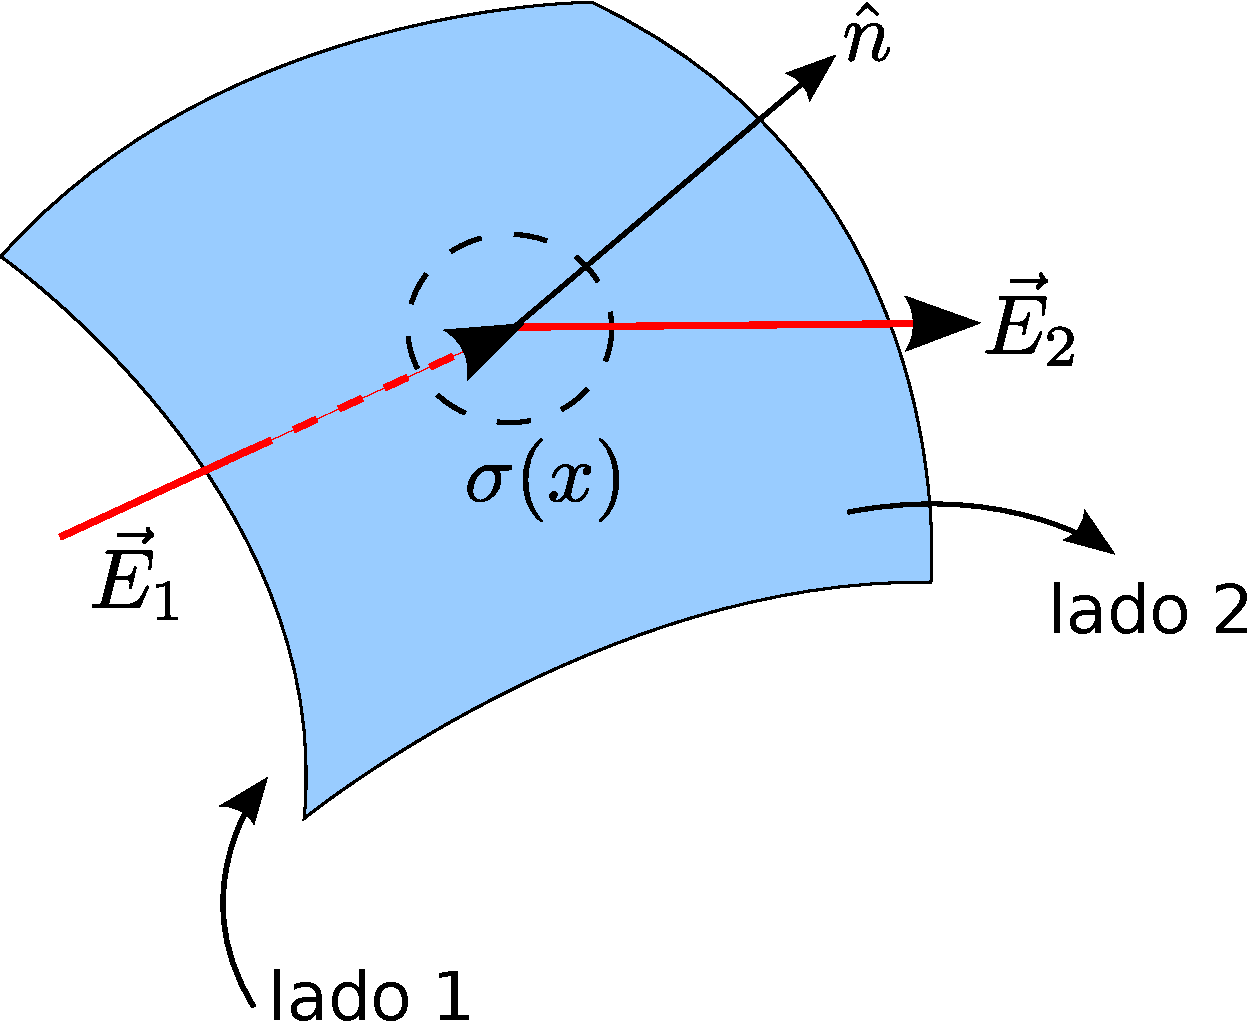
\psfig{file=fig/fig-superficie-frontera.pdf,height=6cm,angle=0}}
\caption{Condiciones de frontera para el campo el'ectrico.}
\label{DSCE1}
\end{figure}
Para estudiar las condiciones que el campo el'ectrico satisface en esta
interfase, aplicamos primero la ley de Gauss, a la superficie gaussiana de la
figura \ref{DSCE2}:
\begin{figure}[!h]
\centerline{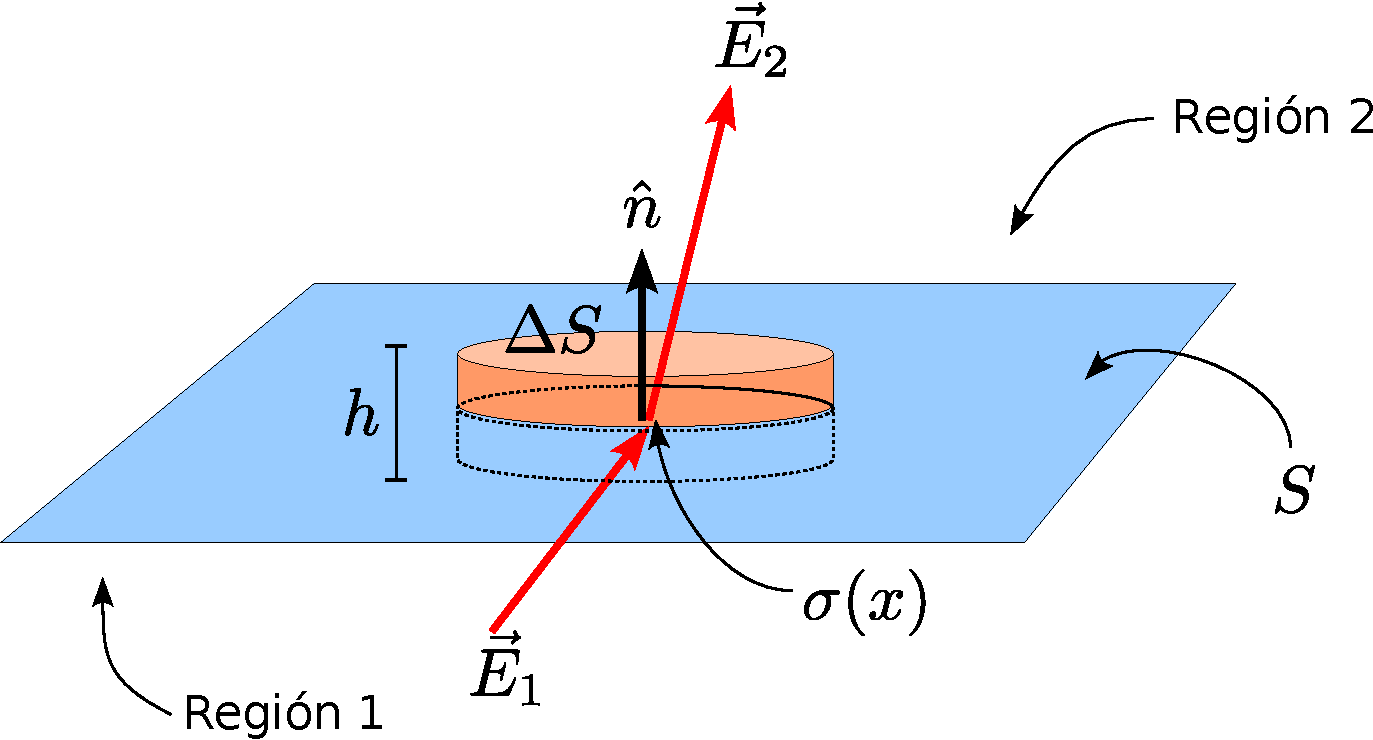
\psfig{file=fig/fig-condicion-borde-electrico-01.pdf,height=5cm,angle=0}}
\caption{Condici'on de frontera para la componente normal del campo el'ectrico.}
\label{DSCE2}
\end{figure}
\begin{eqnarray}
\oint_{S} \vec{E}\cdot d\vec{S}&=&\int_{S_1}
\vec{E}_1\cdot d\vec{S}+\int_{S_2} \vec{E}_2 \cdot d\vec{S}+\int_{S_3}
\vec{E}\cdot d\vec{S}\\
&=& -(\vec{E}_1\cdot\hat{n})\Delta S+(\vec{E}_2\cdot\hat{n})\Delta S+0\\
&=& \frac{\sigma S}{\varepsilon_0},
\end{eqnarray}
donde $\Delta S$ es una superficie, cuyo \textit{vector unitario $\hat{n}$ est'a dirigido
desde la cara $1$ a la cara $2$}, que contiene una densidad de carga
$\sigma(\vec{x})$ $\left[ C/m^2\right]  $, y los campos el'ectricos a
cada lado de la superficie son como se indica en la figura.

Por tanto, obtenemos
\begin{equation}\marginnote{Discontinuidad comp. normal}
\boxed{\vec{E}_2\cdot\hat{n}-\vec{E}_1\cdot\hat{n}=\frac{\sigma}
{\varepsilon_0}.}\label{saltoEn}
\end{equation}

Por otro lado, aplicando (\ref{ointE0}) a la curva de la figura \ref{DSCE3} obtenemos:
\begin{figure}[!h]
\centerline{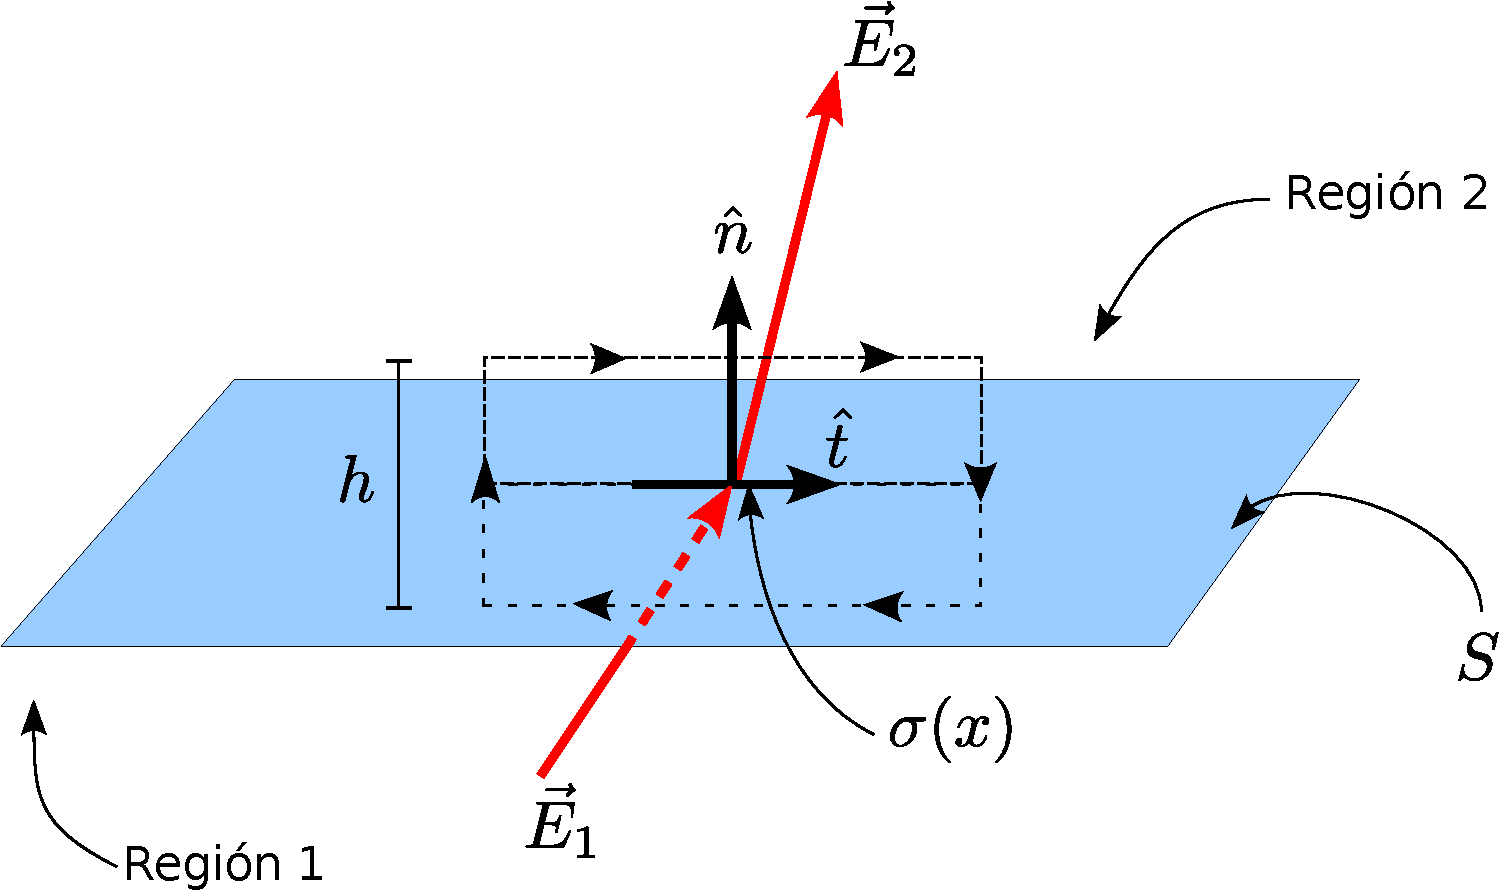
\psfig{file=fig/fig-condicion-borde-electrico-02.pdf,height=5cm,angle=0}}
\caption{Condici'on de frontera para la componente tangencial del campo el'ectrico.}
\label{DSCE3}
\end{figure}
\begin{eqnarray}
 \oint_{\cal C} \vec{E}\cdot d\vec{x}&=&\int_{{\cal C}_1} \vec{E}\cdot
d\vec{x}+\int_{{\cal C}_2} \vec{E}\cdot d\vec{x}+\int_{{\cal C}_3}
\vec{E}\cdot d\vec{x}+\int_{{\cal C}_4} \vec{E}\cdot d\vec{x} \\
&=& -(\vec{E}_1\cdot\hat{t})\ell +(\vec{E}_2\cdot\hat{t})\ell +0+0 \\
&=& 0.
\end{eqnarray}
De aqu'i encontramos que
\begin{equation}\marginnote{Continuidad comp. tangencial}
 \boxed{\vec{E}_2\cdot\hat{t}=\vec{E}_1\cdot\hat{t}.} \label{Etconst}
\end{equation}
Ya que la direcci'on del vector $\hat{t}$ es arbitraria (pero siempre
tangencial a la superficie $S$), la condici'on (\ref{Etconst}) implica que
 \textit{las componentes tangenciales (2 componentes linealmente idependientes) del campo el'ectrico permanecen inalteradas
al cruzar la superficie} $S$.

\subsection{Conductores}

Los \textbf{conductores} son materiales que, aunque est'en
el'ectricamente neutros a nivel macros\-c'o\-pi\-co, poseen
una enorme cantidad de electrones ``libres'' (es decir,  no ligados a
los 'atomos, y que pueden moverse a trav'es del conductor tan pronto como
exista un campo el'ectrico que induzca su movimiento)
aptos para conducir la electricidad. La carga de estos electrones es
neutralizada (a escala macrosc'opica) por la de los protones que est'an en los n\'{u}cleos, que pueden considerarse fijos. Como ejemplo de conductores podemos mencionar a los metales y a los electrolitos (cambi'en conocidos como \textbf{soluciones i'onicas}).

Si un conductor es cargado, o est'a en presencia de cargas externas, los electrones r'apidamente\footnote{Como veremos m'as adelante el \textit{tiempo de relajaci'on} es del orden de $\tau=\varepsilon/\sigma$ donde $\varepsilon$ es la \textit{constante diel'ectrica} del material y $\sigma$ su \textit{conductividad}. Por ejemplo, para el cobre $\tau\approx 10^{-19}$s.} se desplazan hasta una situaci'on de \textit{equilibrio}, es decir, un \textit{estado estacionario}. En este
estado el campo el'ectrico (macrosc'opico) en el interior del conductor debe anularse ya que de otro modo la fuerza sobre ellos ser'ia no nula, induciendo
movimiento. Por tanto, en situaci'on estacionaria $\vec{E}=\vec{0}$ en el
\textit{interior} de los conductores. Como consecuencia de la ley de Gauss, la
densidad de carga en el interior del conductor se anula cuando 'este
alcanza su estado estacionario. En otras palabras, \textit{un conductor en estado estacionario distribuye su carga neta sobre su superficie}.

Aplicando las condiciones de borde (\ref{saltoEn}) y (\ref{Etconst}) a la
interfase del conductor, y tomando en cuenta que en este caso
$\vec{E}_1=\vec{0}$, encontramos que \textit{en cada punto de la superficie (exterior) del conductor}
\begin{equation}\marginnote{Campo fuera de conductor}
 \vec{E}_2(x)=\frac{\sigma(x)}{\varepsilon_0}\hat{n}(x), \label{Econd}
\end{equation}
es decir, que el campo el'ectrico es normal a la superficie, y proporcional a la densidad de carga en cada punto de 'esta. El potencial el'ectrico, por otro lado, es necesariamente constante tanto dentro del conductor como sobre su superficie.

\subsection{Sobre (dis)continuidad de los campos}
 Idealmente, al menos cl'asica y macrosc'opicamente, la distribuci'on de carga descrita por la densidad volum'etrica $\rho(\vec{x})$ debiese ser una funci'on \textit{finita y continua} en todo punto. Como consecuencia, el campo el'ectrico y el potencial ser'ian, de acuerdo a (\ref{cerho}) y (\ref{perho}), tambi'en funciones finitas y cont'inuas. Sin embargo, com'unmente es \textit{conveniente} idealizar la distribuci'on de cargas, considerando que 'esta est'a limitada a una superficie bidimensional (es decir, de secci'on transversal despreciable). Este caso corresponde a considerar una densidad volum'etrica $\rho$ singular (discontinua y divergente)\footnote{Por ejemplo, la densidad volum'etrica correspondiente a una carga distribuida en todo el plano $xy$, con densidad superficial de carga $\sigma(x,y)$ puede escribirse como $\rho(x,y,z)=\sigma(x,y)\delta(z)$.}. En este caso, el campo el'ectrico poseer'a, en general, \textit{discontinuidades} en la superficie donde $\rho$ es singular, tal como analizamos en la secci'on \ref{secCBE}, pero ser'a \textit{finito en todo punto}. El potencial, por otro lado, ser'a una \textit{funci'on continua y diferenciable por tramos}. En resumen, para distribuciones de carga singulares que incluyan distribuciones superficiales de carga, el potencial puede siempre considerarse como una funci'on continua, el campo el'ectrico (proporcional a las derivadas del potencial) puede tener discontinuidades, mientras que las segundas derivadas del potencial (proporcionales a las primeras derivadas del campo el'ectrico y, a trav'es de la ecuaci'on de Poisson (\ref{poisson}), ligadas a la densidad volum'etrica de carga) pueden poseer regiones (superficies) singulares. En el caso de que la distribuci'on de carga se modele incluyendo cargas puntuales o l'ineas de carga, el potencial ya no ser'a finito en todo punto.


\section{Soluci'on de la ecuaci'on de Laplace}
\subsection{Coordenadas Esf'ericas}
Una soluci'on general (finita sobre el eje $z$) de la ecuaci'on de Laplace en coordenadas esf'ericas puede escribirse como:
\begin{equation}
  \boxed{\phi(r,\theta,\varphi) = \sum_{l=0}^\infty\sum_{m=-l}^l\left[
  A_{lm}  r^l + B_{lm}  r^{-(l+1)}\right]  Y_{lm}(\theta,\varphi),}
  \label{est31b}
\end{equation}
donde $A_{lm}$ y $B_{lm}$ son coeficientes constantes. Note que estos
coeficientes son en general complejos.

Si, como caso particular, el potencial tiene simetr'ia axial, es decir no
depende de la coordenada $\varphi$, entonces la expansi'on se reduce a
\begin{eqnarray}
  \phi(r,\theta) &=& \sum_{l=0}^\infty\left[
  A_{l0}  r^l + B_{l0}  r^{-(l+1)}\right]  Y_{l0}(\theta,\varphi) \\
&=&\sum_{l=0}^\infty\left[  A_{l0}  r^l + B_{l0}
r^{-(l+1)}\right]\sqrt{\frac{2l+1}{4\pi}}\,P_l(\cos\theta) ,
\end{eqnarray}
o, equivalentemente,
\begin{equation}\label{phiaxial}
\boxed{\phi(r,\theta)=\sum_{l=0}^\infty\left[  a_l\,  r^l +
\frac{b_l}{r^{l+1}}\right]\,P_l(\cos\theta),}
\end{equation}
donde $a_l$ y $b_l$ son nuevos coeficientes reales constantes.

\subsubsection{Ejemplo: Esfera conductora en un campo el'ectrico externo}\label{sec:esfcond}

Consideramos una esfera conductora de radio $R$ ubicada en un campo externo inicial homog'eneo $\vec{E}_0$. Elegimos los ejes coordenados de modo que el origen coincida con el centro de la esfera y el eje $z$ con la direcci'on del campo externo, es decir, $\vec{E}_0=E_0\hat{z}$.

Luego de ubicar la esfera en el campo externo, las cargas libres en ella se reacomodan r'apidamente. En la situaci'on estacionaria final el campo el'ectrico en el interior de la esfera es nulo, es decir, $\vec{E}=0$ para $r<R$. Como consecuencia directa $\phi=\text{cte.}$ para $r<R$. Podemos elegir esta constante igual a cero, de modo que
\begin{equation}
\phi(r,\theta)=0, \qquad r<R.
\end{equation}
Por otro lado, de acuerdo a (\ref{Econd}) el campo el'ectrico en la superficie externa del conductor es radial, y proporcional a la densidad de carga $\sigma(\theta,\varphi)$. Debido que el sistema es sim'etrico bajo rotaciones en torno a la direcci'on de $\vec{E}$, tendremos que $\phi=\phi(r,\theta)$ y $\sigma=\sigma(\theta)$. Finalmente, fuera de la esfera el potencial satisface la ec. de Laplace, por lo que 'este debe tener la forma general (\ref{phiaxial}). Por lo tanto, para determinar el potencial en todo punto basta determinar los coeficientes (constantes) $a_l$ y $b_l$.

Una condici'on necesaria es que asimpt'oticamente, es decir, para $r\to\infty$, el campo debe tender al campo externo inicial ya que los efectos de las cargas inducidas en la esfera ser'an cada vez menores en puntos cada vez m'as alejados, es decir, $\vec{E}\to\vec{E}_0 $. Esta condici'on es equivalente a 
\begin{equation}
\phi\to -E_0z+\alpha=-E_0r\cos\theta+\alpha .
\end{equation}
Aplicando esta condici'on a la expansi'on (\ref{phiaxial}) encontramos que necesariamente
\begin{equation}
a_0=\alpha, \qquad a_1=-E_0, \qquad a_2=a_3=\cdots =0,
\end{equation}
por lo que el potencial en todo punto se reduce a 
\begin{equation}
\phi(r,\theta)=\alpha -E_0 r\cos\theta +
\sum_{l=0}^\infty\frac{b_l}{r^{l+1}}P_l(\cos\theta), \qquad r\ge R.
\end{equation}
Como el potencial es una funci'on cont'inua, debemos tener que
\begin{equation}
\phi(R,\theta)=\alpha -E_0 R\cos\theta +
\sum_{l=0}^\infty\frac{b_l}{R^{l+1}}P_l(\cos\theta)=0, \qquad \forall \theta.
\end{equation}
De aqu'i, y ya que los polinomios de Legendre son funciones linealmente independientes, encontramos que necesariamente
\begin{equation}
\alpha+\frac{b_0}{R}=0, \qquad -E_0R+\frac{b_1}{R^2}=0, \qquad b_2=b_3=\cdots =0.
\end{equation}
Con esto, el potencial se reduce a
\begin{equation}\label{phialpha}
\phi(r,\theta)=\alpha -E_0 r\cos\theta -\alpha\frac{R}{r}+E_0 \frac{R^3}{r^2}\cos\theta. 
\end{equation}
La constante $\alpha$ es proporcional a la carga neta de la esfera. En efecto, usando (\ref{Econd}) podemos calcular la densidad superficial de carga en la esfera:
\begin{align}
\sigma(\theta) &= \varepsilon_0\, \vec{E}(R,\theta)\cdot\hat{r} \\
&= -\varepsilon_0 \frac{\partial\phi}{\partial r}(R,\theta) \\
&= -\varepsilon_0\left[-E_0\cos\theta+\frac{\alpha}{R}-2E_0\cos\theta\right]\\
&= \varepsilon_0\left[3E_0\cos\theta-\frac{\alpha}{R}\right].
\end{align}
La carga neta de la esfera es entonces
\begin{align}
Q &= \int_S\sigma(\theta)\,dS \\
&= 2\pi R^2 \int_0^\pi \sigma(\theta)\sen\theta\,d\theta \\
&= 2\pi \varepsilon_0R^2 \int_0^\pi \left[3E_0\cos\theta-\frac{\alpha}{R}\right] \sen\theta\,d\theta \\
&= 2\pi \varepsilon_0R^2 \left[ 0-\frac{2\alpha}{R}\right] \\
&= -4\pi \varepsilon_0R \alpha .
\end{align}
En otras palabras, 
\begin{equation}
\alpha=-\frac{Q}{4\pi \varepsilon_0}\frac{1}{R}.
\end{equation}
Con este resultado, el potencial (\ref{phialpha}) puede escribirse como 
\begin{equation}
\phi(r,\theta)=-\frac{Q}{4\pi\varepsilon_0 R}+\frac{Q}{4\pi\varepsilon_0}\frac{1}{r} -E_0 \left(1-\frac{R^3}{r^3}\right)r\cos\theta.
\end{equation}
Como vemos, los primeros dos t'erminos son independientes del campo externo y representan el potencial de la carga neta de la esfera (que hemos supuesto aislada). El tercer t'ermino es el campo externo inicial y por lo tanto el 'ultimo t'ermino describe el campo el'ectrico inducido producto de la polarizaci'on de la esfera conductora.
\begin{figure}[!h]
\centerline{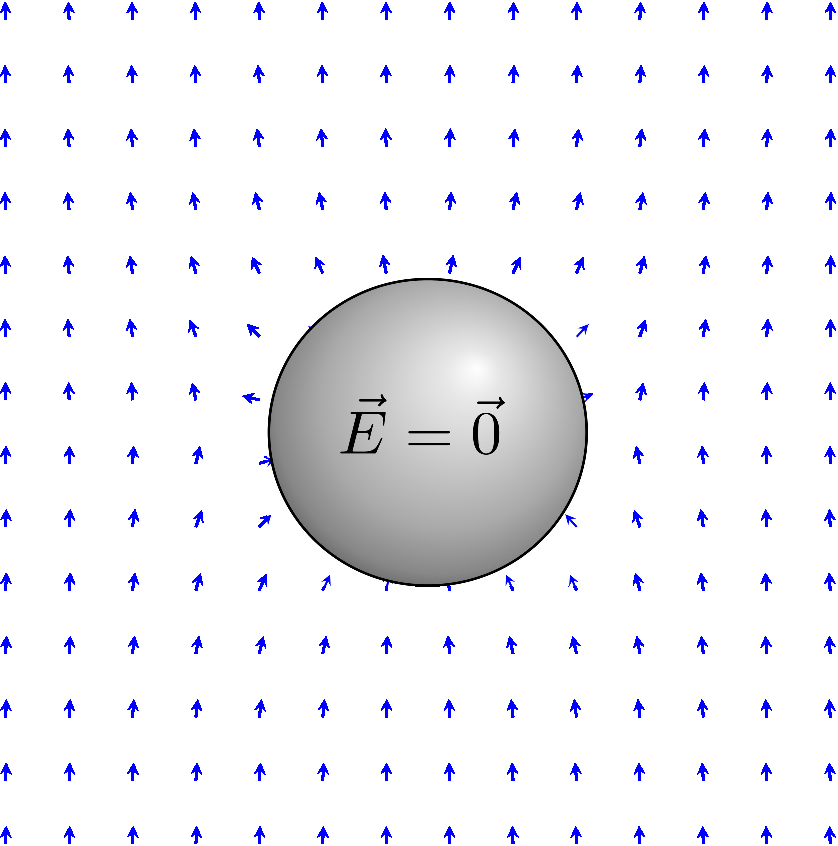
\psfig{file=fig/fig-esfera-conductora-campo-externo.pdf,height=5.5cm,angle=0}
\hspace{1cm}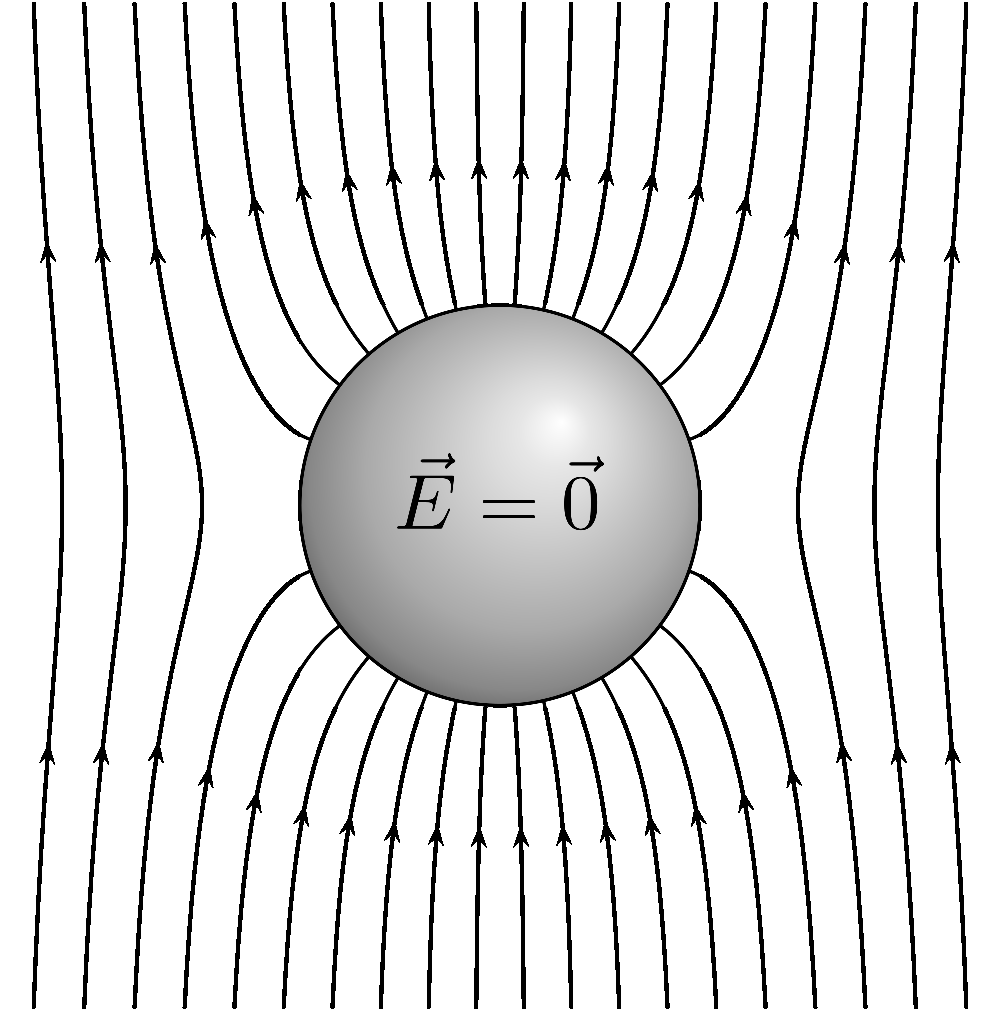
\psfig{file=fig/fig-esfera-conductora-campo-externo-2.pdf,height=5.5cm,angle=0}}
\caption{Campo el'ectrico de una esfera conductora neutra en un campo el'ectrico externo. El gr'afico de la izquierda (normalizado) fue creado usando \href{https://github.com/gfrubi/electrodinamica/blob/master/figuras-editables/fig-esfera-conductora-campo-externo-raw.py}{este script} Python. La figura de la derecha fue generada usando \href{http://commons.wikimedia.org/wiki/User:Geek3/VectorFieldPlot}{VectorFieldPlot}, a partir de \href{http://commons.wikimedia.org/wiki/File:VFPt_superconductor_ball_E-field.svg}{este} archivo original.}
\label{fig:ecce}
\end{figure}
El campo el'ectrico es entonces dado por
\begin{equation}
\vec{E}(r,\theta)=E_r\hat{r}+E_\theta\hat{\theta},
\end{equation}
con 
\begin{equation}
E_r=\frac{Q}{4\pi\varepsilon_0}\frac{1}{r^2}+E_0 \left(1+2\frac{R^3}{r^3}\right)\cos\theta, \qquad E_\theta=-E_0 \left(1-\frac{R^3}{r^3}\right)\sen\theta .
\end{equation}
En la figura \ref{fig:ecce} se muestra la forma de este campo, en el caso en que $Q=0$.


%\subsection{Coordenadas Cil'indricas}

%\subsection{Coordenadas Cartesianas}

 \section{Soluci'on de la ecuaci'on de Poisson} 
 \subsection{Soluci'on en t'erminos de Funciones de Green*}
 La ecuaci'on de Poisson \eqref{poisson} para el potencial es una \textit{EDP lineal el'iptica inhomog'enea}. Una forma de encontrar soluciones de este tipo de ecuaciones es usando el m'etodo de las \textit{funciones de Green}. En nuestro caso, se dice que $G(\vec{x},\vec{x}')$ es una funci'on de Green del operador Laplaciano si satisface
\begin{equation}\label{EDPG}
\nabla^2G(\vec{x}',\vec{x})=\delta(\vec{x}-\vec{x}').
\end{equation} 
Si se conoce una funci'on de Green entonces la soluci'on de la ecuaci'on de Poisson para el potencial en una regi'on $V$ puede expresarse de la forma siguiente:
\begin{align}
\phi(\vec{x}) &= -\frac{1}{\varepsilon_0}\int_VG(\vec{x},\vec{x}')\rho(\vec{x}')dV'+\oint_{\partial V}\left[\phi(\vec{x}')\vec\nabla' G(\vec{x},\vec{x}')-G(\vec{x},\vec{x}')\vec\nabla'\phi(\vec{x}')\right]\cdot d\vec{S}' \\
&=  -\frac{1}{\varepsilon_0}\int_VG(\vec{x},\vec{x}') \rho(\vec{x}')dV'+\oint_{\partial V}\left[\phi(\vec{x}')\frac{\partial G}{\partial n'}(\vec{x},\vec{x}')-G(\vec{x},\vec{x}')\frac{\partial\phi}{\partial n'}(\vec{x}')\right]dS'
\end{align}
Introduciendo el campo el'ectrico en el segundo t'ermino del lado derecho podemos escribir
\begin{equation}\label{solPoisson}
\phi(\vec{x})= -\frac{1}{\varepsilon_0}\int_VG(\vec{x},\vec{x}') \rho(\vec{x}')dV'+\oint_{\partial V}\left[\phi(\vec{x}')\frac{\partial G}{\partial n'}(\vec{x},\vec{x}')+G(\vec{x},\vec{x}')E_n(\vec{x}')\right]dS',
\end{equation}
donde $E_n:=\vec{E}\cdot\hat{n}$ es la componente del campo el'ectrico normal a la superficie $\partial V$ (con $\hat{n}$ orientado hacia el exterior del volumen $V$).

Por otro lado, la funci'on de Green no es 'unica. Si $G_1(\vec{x},\vec{x}')$ es una funci'on de Green entonces $G_2(\vec{x},\vec{x}')=G_1(\vec{x},\vec{x}')+H(\vec{x},\vec{x}')$ tambi'en lo ser'a si $H$ es una soluci'on del problema homog'eneo: en nuestro caso de la ecuaci'on de Laplace, $\nabla^2H(\vec{x},\vec{x}')=0$. Esta arbitrariedad en la definici'on de la funci'on de Green es de hecho una ventaja, puesto que en general no se tiene informaci'on \textit{simult'anea} del potencial y la componente normal del campo en la frontera $\partial V$. Por esto, es conveniente elegir una funci'on de Green de modo que los t'erminos del lado derecho de \eqref{solPoisson} puedan efectivamente ser evaluados. Por ejemplo, si se conoce el potencial\footnote{condici'on de borde tipo Dirichlet.} en $\partial V$ (t'ipicamente, en situaciones donde $\partial V$ coincide con la superfice de conductores conectados a bater'ias suministrando una diferencia de potencial conocida) entonces es conveniente usar una \textit{funci'on de Green que se anule en la frontera}, $G(\vec{x},\vec{x}')=0$, $\forall$ $\vec{x}'\in\partial V$. En este caso, la soluci'on se reduce a
\begin{equation}\label{solPoissonDirichlet}
\phi(\vec{x})= -\frac{1}{\varepsilon_0}\int_VG(\vec{x},\vec{x}') \rho(\vec{x}')dV'+\oint_{\partial V}\phi(\vec{x}')\frac{\partial G}{\partial n'}(\vec{x},\vec{x}')dS',
\end{equation}
 Por otro lado, si se conoce la componente normal del campo en la frontera\footnote{condici'on de borde tipo Neumann.} (por ejemplo, en situaciones donde se dispone de informaci'on sobre la densidad de carga superficial en $\partial V$) entonces parece conveniente usar una funci'on de Green tal que su derivada normal sobre la frontera sea nula. Lamentablemente, esta condici'on \textit{no es posible de implementar} ya que necesariamente\footnote{Use el teorema de Gauss sobre la integral de volumen de \eqref{EDPG} para verificar esto!.} debe cumplirse que
\begin{equation}\label{intGn}
\oint_{\partial V}\frac{\partial G}{\partial n'}dS'=1.
\end{equation}
Una condici'on un poco menos restrictiva, y factible de implementar consistentemente, es imponer que la derivada normal de la funci'on de Green sea \textit{constante en la frontera}. Entonces, \eqref{intGn} requiere que
\begin{equation}
\frac{\partial G}{\partial n'}(\vec{x},\vec{x}')=\frac{1}{S}, \qquad \vec{x}'\in\partial V,
\end{equation}
donde $S$ es el 'area total de la frontera, $S:=\oint_{\partial V} dS$. En este caso, la soluci'on para el potencial adopta la forma
\begin{equation}
\phi(\vec{x})= \left\langle\phi\right\rangle_S-\frac{1}{\varepsilon_0}\int_VG(\vec{x},\vec{x}') \rho(\vec{x}')dV'+\oint_{\partial V}G(\vec{x},\vec{x}')E_n(\vec{x}')dS',
\end{equation}
donde
\begin{equation}
\left\langle\phi\right\rangle_S:=\frac{1}{S}\oint_{\partial V}\phi(\vec{x}')\,dS'
\end{equation}
es el \textit{valor promedio del potencial sobre} $\partial V$.

Finalmente, la funci'on de Green m'as conocida del operador Laplaciano es dada por
\begin{equation}
G(\vec{x}-\vec{x}')=-\frac{1}{4\pi}\frac{1}{|\vec{x}-\vec{x}'|}.
\end{equation}
Esta funci'on de Green particular posee las propiedades adicionales de ser sim'etrica bajo rotaciones respecto al punto $\vec{x}'$, depender s'olo de la diferencia $\vec{x}-\vec{x}'$ y de anularse en el infinito (para todo valor finito de $\vec{x}'$). Debido a estas propiedades est'a directamente relacionada con la soluci'on de la ecuaci'on de Poisson en el caso en que la regi'on $V$ cubre todo el espacio y se asume que el campo el'ectrico se anula en el infinito\footnote{m'as r'apido que $1/r$, es decir, tal que $\lim_{|x|\to\infty}|\vec{E}|r=0$.}, de modo que el potencial se reduce a
\begin{equation}
\phi(\vec{x})= \left\langle\phi\right\rangle_\infty+\frac{1}{4\pi\varepsilon_0}\int_V\frac{\rho(\vec{x}')}{|\vec{x}-\vec{x}'|}dV'.
\end{equation}

\subsection{Unicidad de la soluci'on}\label{sec:uniP}
A continuaci'on probaremos que \textit{la soluci'on de la ecuaci'on de Poisson es 'unica} (salvo una constante aditiva), en una regi'on $V$, para valores dados del potencial \textit{o de la componente normal del campo} en la frontera\footnote{Condiciones de borde tipo Dirichlet o tipo Neumann, respectivamente.} $\partial V$. Para esto, asumimos que existen dos soluciones distintas de \eqref{poisson} en $V$, $\phi_1(\vec{x})$ y $\phi_1(\vec{x})$, que \textit{satisfacen las mismas condiciones de borde}, es decir, su valor es conocido en $\partial V$ o bien su derivada normal es conocida en esta frontera.

Definimos la diferencia $U(\vec{x}):=\phi_1(\vec{x})-\phi_2(\vec{x})$ que ser'a entonces una soluci'on de la ecuaci'on de Laplace, $\nabla^2U=0$. En la frontera $\partial V$ esta funci'on satisface $U=0$ o bien ${\partial U}/{\partial n}=0$, ya que asumimos que $\phi_1$ y $\phi_2$ satisfacen las mismas condiciones de borde (tipo Dirichlet, o bien tipo Neumann). Usamos ahora la identidad\footnote{Esta identidad es un caso particular de la as'i llamada \textit{primera identidad de Green}.}
\begin{equation}
 \int_V\left[\left|\vec\nabla U\right|^2+U\nabla^2U\right]  \,dV
 \equiv\oint_SU\frac{\partial U}{\partial n}\,dS,
 \end{equation}
que puede ser verificada f'acilmente usando el teorema de Gauss. En nuestro caso, dada la EDP y las condiciones de borde que $U$ satisface, la identidad implica que
\begin{equation}
 \int_V\left|\vec\nabla U\right|^2dV=0.
\end{equation}
Como consecuencia la funci'on $U$ debe ser \textit{constante}\footnote{En principio, esto ser'ia v'alido excepto (a lo sumo) en un conjunto de medida cero. Sin embargo, esta posibilidad queda descartada si el potencial es una funci'on continua.}, por lo que las dos soluciones $\phi_1$ y $\phi_2$ s'olo pueden diferir por una constante, representando la misma soluci'on f'isica\footnote{M'as a'un, para condiciones de borde tipo Dirichlet, esta constante es necesariamente nula.}.

Es importante notar que este resultado implica que, en general, es inconsistente intentar encontrar una soluci'on de la ecuaci'on de Poisson \textit{imponiendo simult'aneamente el valor del potencial y de su derivada normal en la frontera}.

Note que los teoremas anteriores implican que el campo el'ectrost'atico en una regi'on $V$ queda totalmente determinado por la densidad de carga en el interior del volumen $V$, y por las condiciones de borde en la frontera $\partial V$. Una de las m'ultiples consecuencias de este hecho es que el campo al interior de un volumen de forma arbitraria, cuya frontera es mantenida a un potencial fijo (por ejemplo, por medio de un conductor puesto ``a tierra'') es \textit{independiente de la distribuci'on de cargas en el exterior}. De esta forma, es posible aislar una regi'on de las influencias el'ectricas externas (``jaula de Faraday'').


\section{M'etodo de las im'agenes}
Como vimos la secci'on \ref{sec:uniP}, la soluci'on de la ecuaci'on de Poisson, que determina el potencial electrost'atico y por lo tanto tambi'en el campo el'ectrico, es 'unica dadas las condiciones de borde apropiadas. Debido a esto, si
obtenemos, \textit{por cualquier m'etodo}, una soluci'on que respete las condiciones de
borde dadas, 'esta es \textit{la} soluci'on del problema. El \textit{m'etodo de
las im'agenes} suministra un procedimiento para encontrar una soluci'on en
casos donde el sistema contiene conductores (perfectos) a potencial constante
(t'ipicamente, ``puestos a tierra'') y la geometr'ia de los conductores y las
cargas es simple. Para ello, se introducen \textit{cargas ficticias} en
posiciones apropiadas tales que el campo creado por el sistema de cargas reales
+ ficticias satisface las condiciones de borde.

En otras palabras, el m'etodo de las im'agenes se basa en el hecho que la
soluci'on para el campo el'ectrico en una regi'on finita $V$ con una
distribuci'on de carga conocida y potenciales dados en su superficie
$\partial V$ pueden ser los mismos (\underline{en $V$}) que los campos generados por la
misma distribuci'on de carga en $V$ \textit{y por otra distribuci'on de carga
diferente fuera de $V$}. Por esto, para solucionar el problema ``real'', en el
que la distribuci'on de carga en $V$ y los potenciales en $\partial V$ son conocidos, se
puede considerar el problema ``ficticio'' de encontrar las cargas ``imagenes''
fuera de $V$ tales que la distribuci'on de cargas total (reales e im'agenes)
satisfaga las condiciones de contorno en $\partial V$. Los campos as'i encontrados son
soluci'on del problema original, dentro (pero \underline{no} fuera) de $V$. Como veremos, el m'etodo de las im'agenes b'asicamente provee un m'etodo heur'istico para encontrar la funci'on de Green apropiada a las condiciones de borde de un cierto problema f'isico.



\subsection{Conductor plano}
\begin{figure}[!h]
\centerline{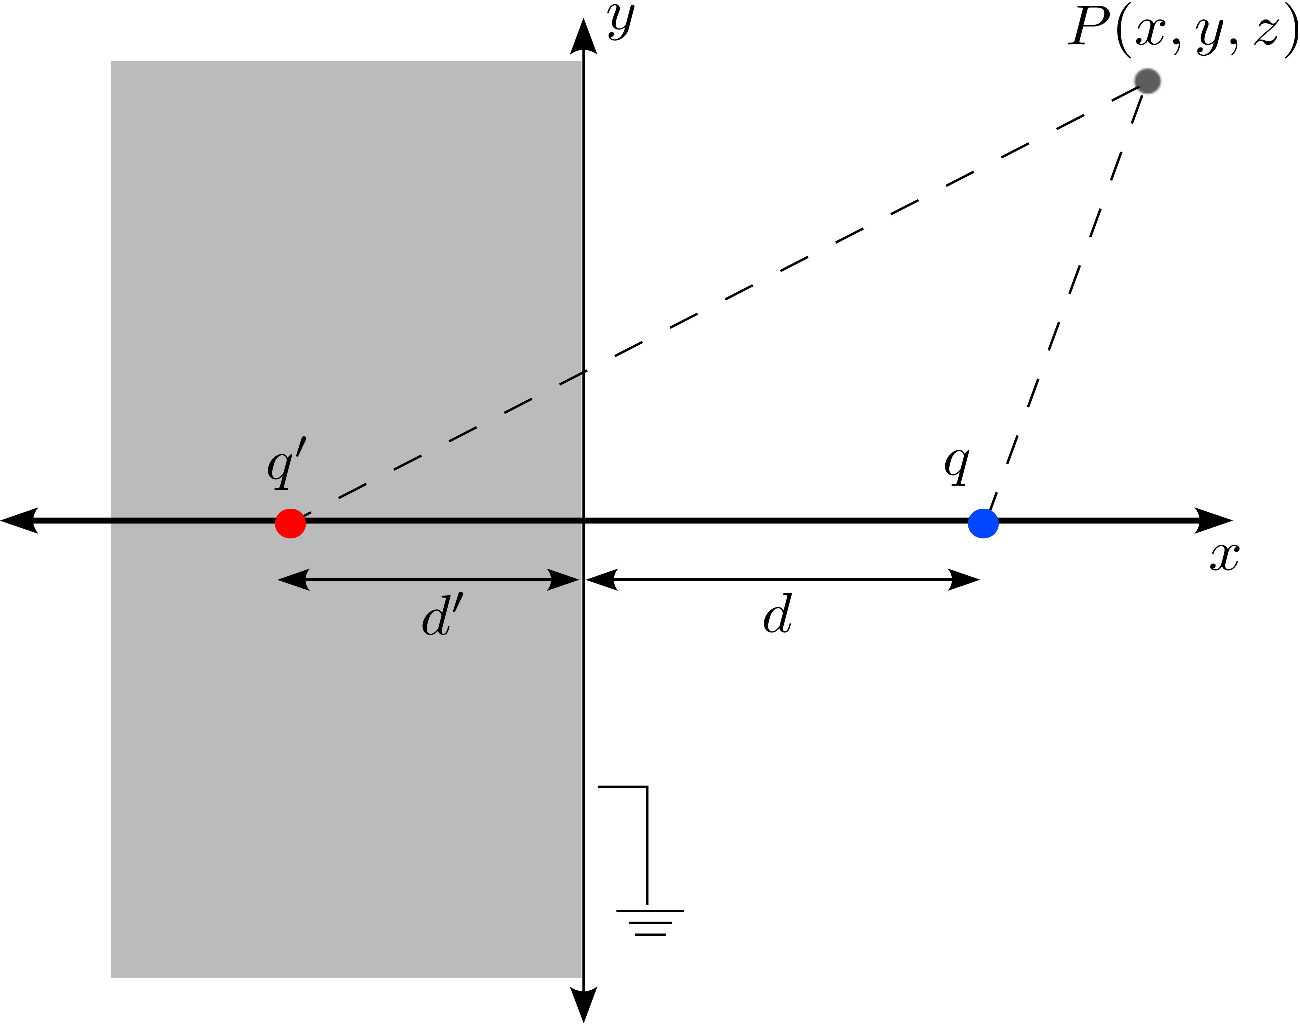
\psfig{file=fig/fig-carga-imagen-01.pdf,height=6cm,angle=0}}
\caption{Conductor plano, carga real $q$ e imagen $q'$.}
\label{ci01}
\end{figure}
Consideremos la situaci'on donde una carga puntual $q$ se encuentra a una distancia $d$ de un plano conductor (infinito) ``puesto a tierra'' (de modo que su potencial es igual al potencial en el infinito, elegido como $\phi_\infty=0$). Eligiendo los ejes coordenados como lo indica la figura \ref{ci01}, tendremos que en la situaci'on estacionaria $\phi=0$ para $x\le 0$. Usando el m'etodo de las im'agenes resolvemos el problema equivalente obtenido al reemplazar el plano conductor por una carga ficticia (imagen) $q'$ ubicada en la posici'on $x=-d'<0$. El potencial de la condiguraci'on de carga real m'as carga imagen es entonces
\begin{equation}
 \phi(x)=\frac{1}{4\pi\varepsilon_0}\left[\frac{q}{\sqrt{(x-d)^2+y^2+z^2}}+\frac
{q'}{\sqrt{(x+d')^2+y^2+z^2}}\right].
\end{equation}
La condici'on que $\phi=0$ sobre el plano, es decir, para todo punto con $x=0$,
se satisface s'olo si
\begin{equation}
 d'=d, \qquad q'=-q.
\end{equation}
Por lo tanto, la soluci'on para el potencial en todo punto con $x\ge 0$ es dada por
\begin{equation}
 \phi(x)=\frac{q}{4\pi\varepsilon_0}\left[\frac{1}{\sqrt{(x-d)^2+y^2+z^2}}-\frac
{1}{\sqrt{(x+d)^2+y^2+z^2}}\right], \qquad x\ge 0.
\end{equation}
\begin{center}
\begin{figure}[H]
\centerline{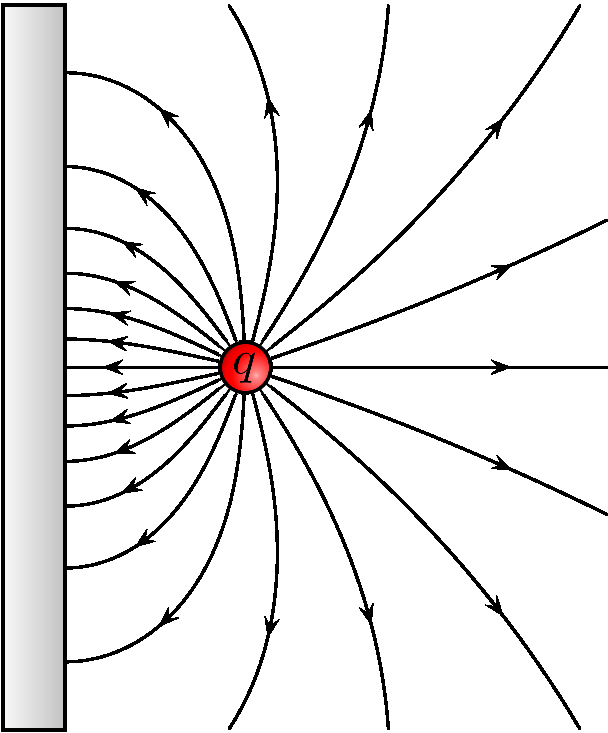
\psfig{file=fig/fig-metodo-imagen-plano-01.pdf,height=4.5cm,angle=0}
\hspace{2cm}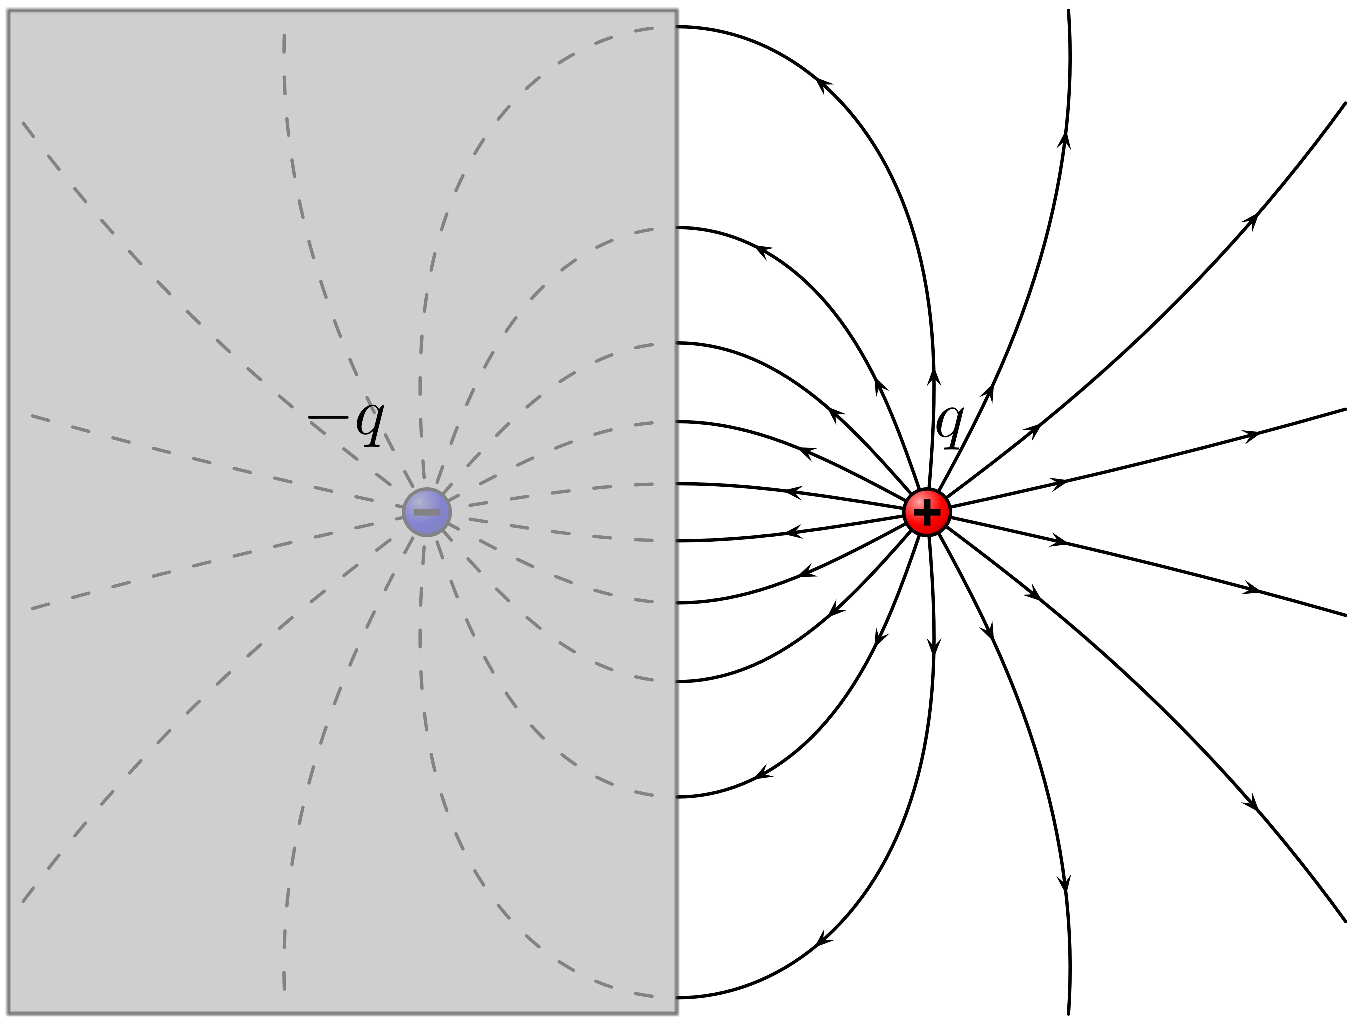
\psfig{file=fig/fig-metodo-imagen-plano-02.pdf,height=4.5cm,angle=0}}
\caption{Campo el'ectrico de plano conductor (puesto a Tierra) y carga puntual. 
Figuras adaptadas de  \href{http://commons.wikimedia.org/wiki/File:VFPt_image_charge_plane_horizontal.svg}{este} y \href{http://commons.wikimedia.org/wiki/File:VFPt_image_charge_plane.svg}{este} archivo original.}
\label{fig:pyc}
\end{figure}
\end{center}
La densidad de carga inducida en el conductor puede calcularse usando
\begin{equation}
 \sigma(y,z)=\varepsilon_0
\vec{E}\cdot\hat{n}=-\varepsilon_0\left.(\partial_x\phi)\right|_{x=0}
\end{equation}
que, luego de algo de 'algebra, resultar ser
\begin{equation}
 \sigma(y,z)=-\frac{q}{2\pi}\frac{d}{(d^2+y^2+z^2)^{3/2}}.
\end{equation}
Por otro lado, la fuerza que ejerce el plano sobre la carga puede ser calculada usando
\begin{equation}
\vec{F}_q=q\vec{E}',
\end{equation}
donde $\vec{E}'$ es el campo \textit{externo} que act'ua sobre $q$, es decir, el campo
determinado por el potencial
\begin{equation}
 \phi'(x)=-\frac{q}{4\pi\varepsilon_0}\frac{1}{\sqrt{(x+d)^2+y^2+z^2}},
\qquad x>0,
\end{equation}
evaluado en la posici'on en que se ubica la carga $q$, es decir,
\begin{eqnarray}
 \vec{F}_q&=&-q(\vec{\nabla}\phi')|_{\vec{x}=d\hat{x}} \\
&=&-\frac{q^2}{16\pi\varepsilon_0d^2}\,\hat{x}.
\end{eqnarray}
Note que esta fuerza es la misma que ejerce(r'ia) la carga imagen sobre la carga real.

\subsection{Conductor esf'erico}
\begin{figure}[!h]
\centerline{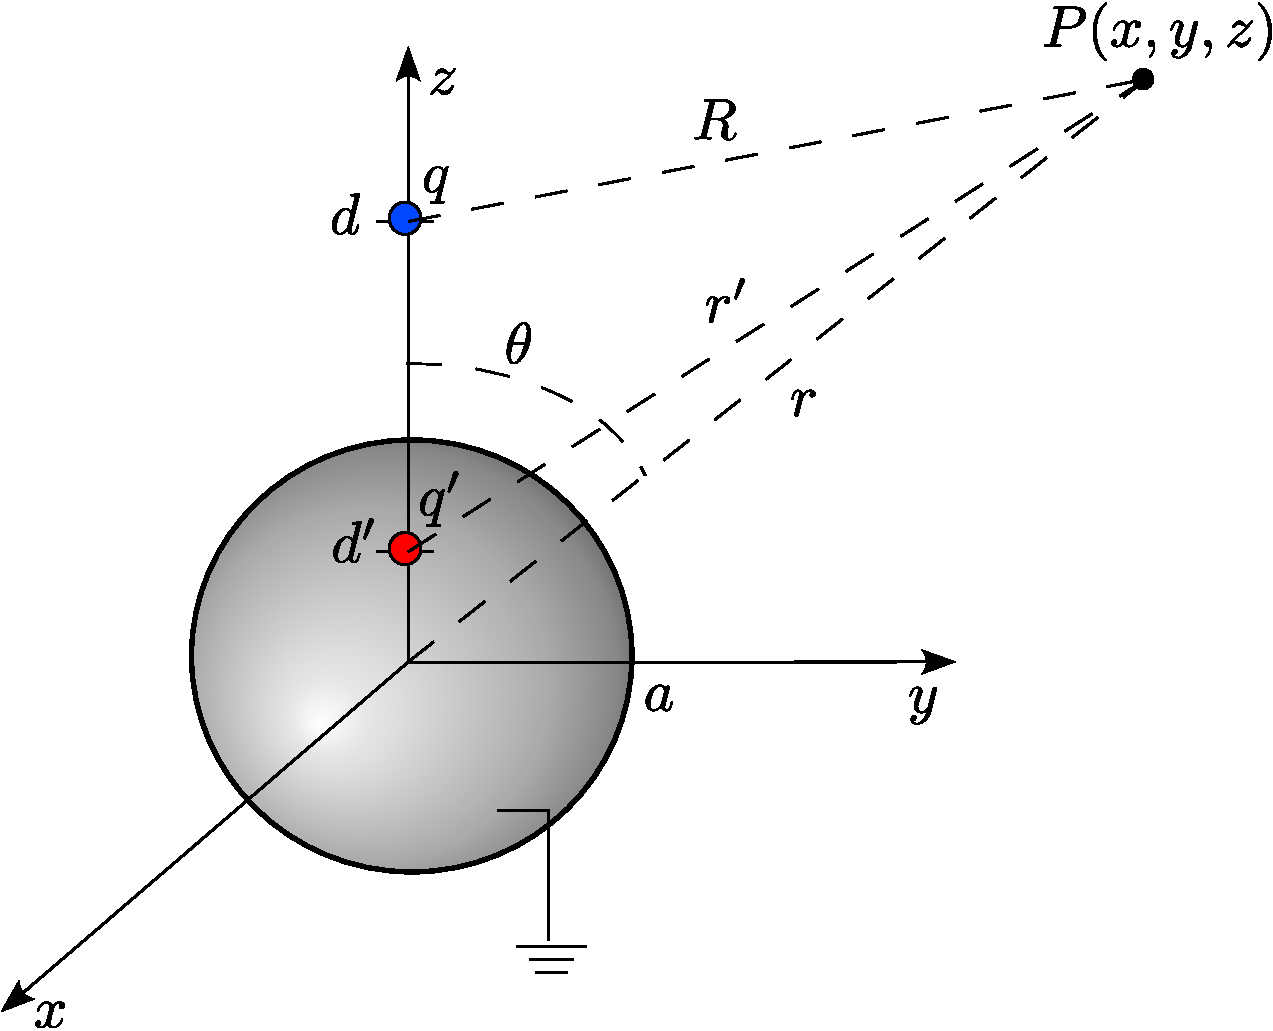
\psfig{file=fig/fig-carga-imagen-02.pdf,height=6cm,angle=0}}
\caption{Conductor esf'erico, carga real $q$ e imagen $q'$.}
\label{ci02}
\end{figure}
En este caso, consideramos el sistema formado por un conductor esf'erico, de radio $a$, ``puesto a tierra", de modo que su potencial $\phi=\phi_\infty\stackrel{!}{=}0$, y una carga puntual $q$ ubicada a una distancia $d$ del centro del conductor. El campo el'ectrico fuera del conductor es equivalente al campo producido por la carga real $q$ y una carga imagen de magnitud $q'$ ubicada dentro de la esfera, a una distancia $d'$ de su centro. 

En efecto, el potencial de la carga real y la carga imagen, de acuerdo a las posiciones indicadas en la figura \ref{ci02}, es dado por
\begin{equation}
 \phi(r,\theta)=\frac{1}{4\pi\varepsilon_0}\left[\frac{q}{\sqrt{
r^2+d^2-2dr\cos\theta } } +\frac{q'}{\sqrt{r^2+d'^2-2d'r\cos\theta}}\right]
\end{equation}
Puede verificarse r'apidamente que la condici'on que $\phi=0$ sobre la esfera, para todo punto con $r=a$, se satisface s'olo si
\begin{equation}
 d'=\frac{a^2}{d}, \qquad q'=-q\frac{a}{d}.
\end{equation}
Por lo tanto, la soluci'on para el potencial en todo punto exterior a la
esfera conductora es dada por
\begin{equation}\label{phice}
 \phi(r,\theta)=\frac{q}{4\pi\varepsilon_0}\left[\frac{1}{\sqrt{
r^2+d^2-2dr\cos\theta}}
-\frac{a}{\sqrt{a^4+r^2d^2-2a^2dr\cos\theta}}\right], \qquad r\ge a .
\end{equation}
\begin{center}
\begin{figure}[H]
\centerline{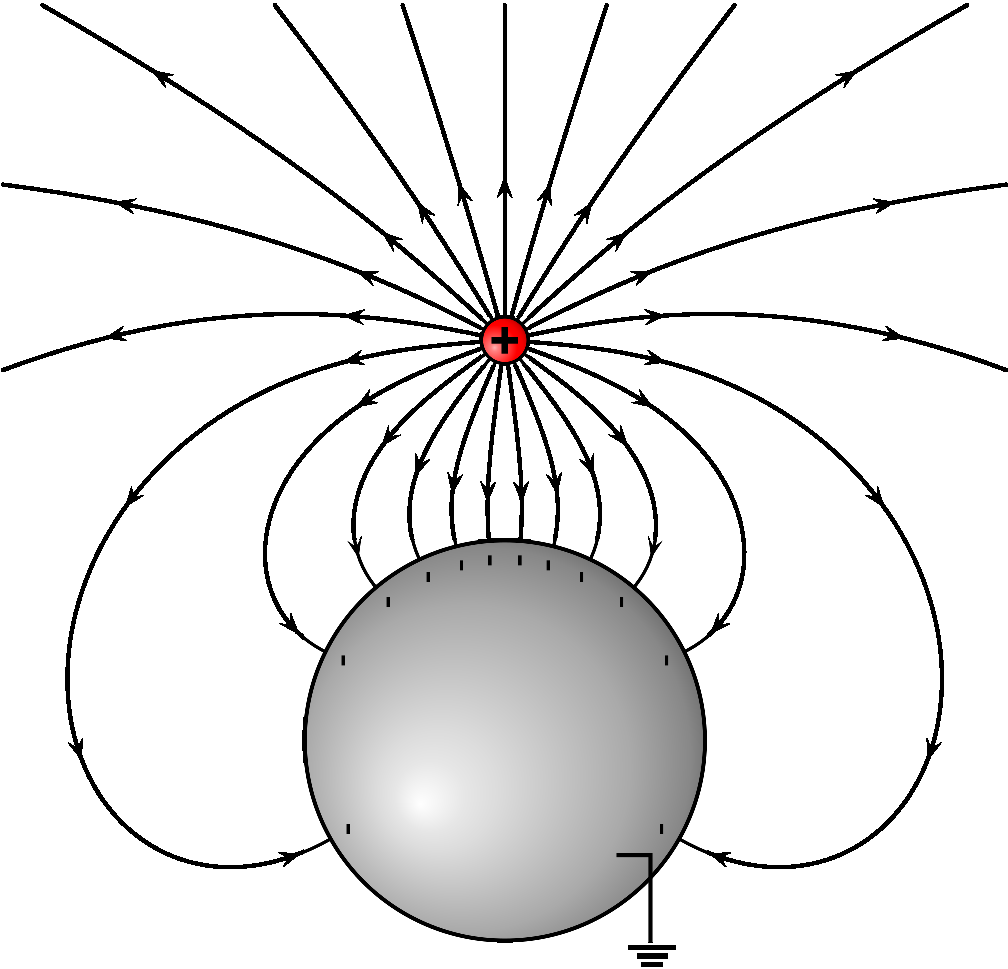
\psfig{file=fig/fig-metodo-imagen-esfera-01.pdf,height=5cm,angle=0}
\hspace{2cm}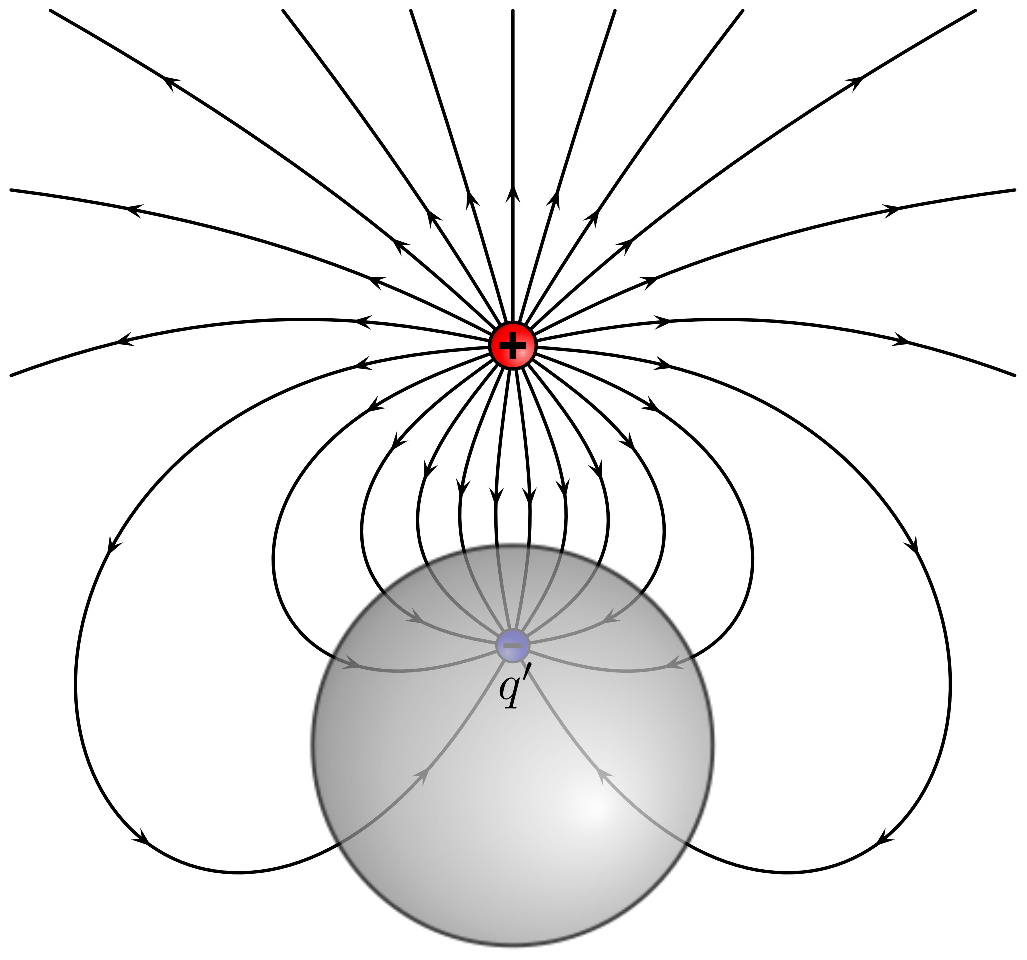
\psfig{file=fig/fig-metodo-imagen-esfera-02.pdf,height=5cm,angle=0}}
\caption{Campo el'ectrico de esfera conductora (puesta a Tierra) y carga puntual. 
Figuras adaptadas a partir de  \href{http://commons.wikimedia.org/wiki/File:VFPt_metal_ball_grounded.svg}{este} y \href{http://commons.wikimedia.org/wiki/File:VFPt_metal_ball_grounded_transparent.svg}{este} archivo original.}
\label{fig:eyc}
\end{figure}
\end{center}
La densidad de carga inducida en la esfera conductora puede calcularse usando
\begin{equation}\label{sce}
 \sigma(\theta)=\varepsilon_0\vec{E}\cdot\hat{n}
=-\varepsilon_0\left.(\partial_r\phi)\right|_{r=a}.
\end{equation}
Reemplazando (\ref{phice}) en (\ref{sce}) encontramos que
\begin{equation}
 \sigma(\theta)=-\frac{q}{4\pi}\frac{1}{ad}\frac{1-\frac{a^2}{d^2
}}{\left[1+\left(\frac{a}{d}\right)^2-2\left(\frac{a}{d}\right)\cos\theta\right]
^{3/2}}.
\end{equation}
La carga total inducida en la esfera es entonces
\begin{equation}
 Q_{\rm ind}=\oint\sigma\,dS=2\pi
a^2\int_0^\pi\sigma(\theta)\sin\theta\,d\theta=-q\frac{a}{d}.
\end{equation}
Note que necesariamente la esfera debe tener una carga neta (igual a la carga imagen) para que $\phi=0$ en su superficie.

Finalmente, la fuerza que la esfera ejerce sobre la carga es dada por
\begin{equation}
\vec{F}_q=-\frac{q^2}{4\pi\varepsilon_0}\frac{a}{d}\frac{1}{(d'-d)^2}\,
\hat{z}=-\frac { q^2 }{4\pi\varepsilon_0}\frac{ad}{(a^2-d^2)^2}\,\hat{z}.
\end{equation}

\subsection{Conductor Cil'indrico}
\begin{figure}[!h]
\centerline{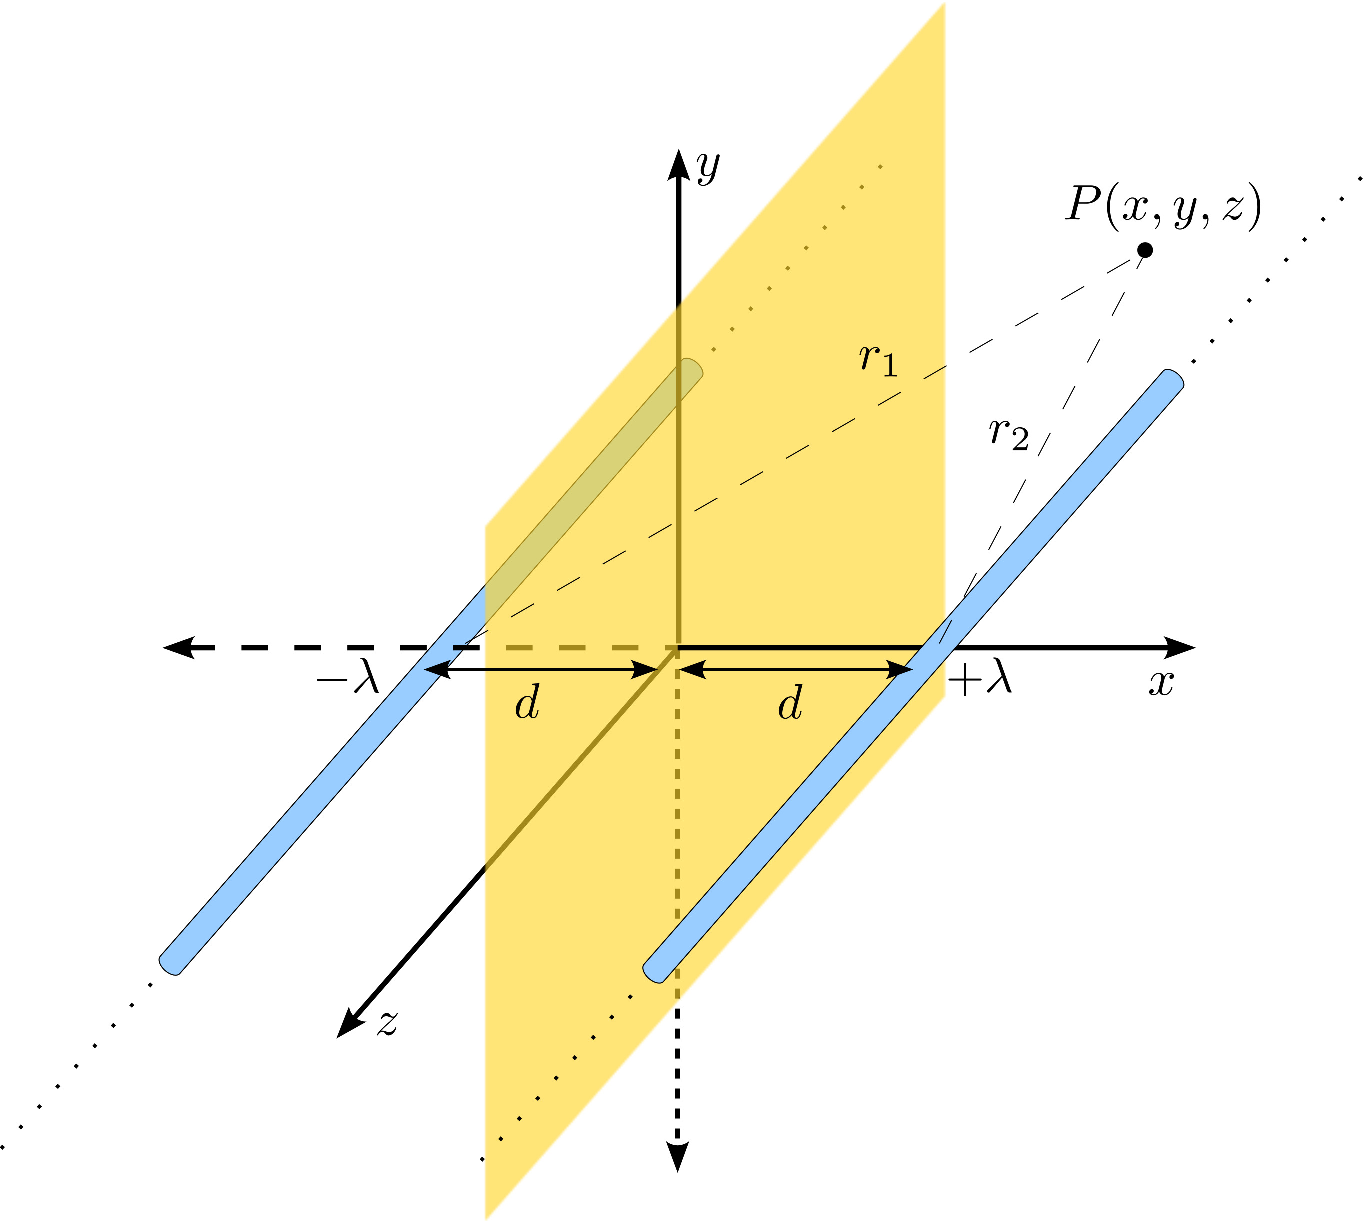
\psfig{file=fig/fig-metodo-imagenes-cilindros-01.pdf,height=6cm,angle=0}}
\caption{Conductor cil'indrico, l'ineas de densidad $\lambda$ y $-\lambda$.}
\label{ci03}
\end{figure}
Consideremos ahora el campo generado por dos l'ineas (infinitas) de carga, con
densidades lineales de carga $\lambda$ y $-\lambda$, situadas en $x=+d$ y
$x=-d$, respectivamente. Ver figura \ref{ci03}.

El potencial en un punto cualquiera fuera de las l'ineas de carga es dado por
\begin{equation}
 \phi(x,y)=\frac{\lambda}{2\pi\varepsilon_0}\ln\left(\frac{r_1}{r_2}
\right)=\frac{\lambda}{4\pi\varepsilon_0}\ln\left(\frac{r_1^2}{r_2^2}
\right)=\frac{\lambda}{4\pi\varepsilon_0}\ln\left(\frac{(x+d)^2+y^2}{
(x-d)^2+y^2}\right).
\end{equation}

Estudiemos la ubicaci'on de las superficies equipotenciales de esta
configuraci'on de cargas. Por simplicidad (de c'alculo), consideraremos las superficies con $\phi=\phi_0=\text{cte.}$, con
\begin{equation}
 \phi_0:=\frac{\lambda}{2\pi\varepsilon_0}\ln M, \label{phi0M}
\end{equation}
donde $M>0$ es una constante adimensional.  Con esto, las superficies $\phi=\phi_0$
corresponden a los puntos que satisfacen
\begin{equation}
 \frac{(x+d)^2+y^2}{(x-d)^2+y^2}=M^2. \label{equip1}
\end{equation}
Luego de un poco de 'algebra encontramos que, si $M\neq 1$, (\ref{equip1}) es
equivalente a
\begin{equation}
 \left[x-\frac{d(1+M^2)}{M^2-1}\right]^2+y^2=\frac{4M^2d^2}{(1-M^2)^2},
\end{equation}
que es la ecuaci'on de un cilindro (una circunsferencia en el plano $xy$),
centrado en las coordenadas $(x_{\rm c},y_c)$ y con radio $R$, dados por
\begin{equation}
 x_{\rm c}=\frac{d(1+M^2)}{M^2-1}, \qquad y_c=0, \qquad R=\frac{2Md}{|1-M^2|}.
\label{cilim}
\end{equation}
Vemos de aqu'i que (asumiendo $\lambda>0$) $x_{\rm c}<-d$ y $\phi_0<0$ si $M<1$,
mientras que $x_{\rm c}>d$ y $\phi_0>0$ si $M>1$.

Por otro lado, si $M=1$, entonces la superficie equipotencial es el plano
definido por $x=0$, es decir, el plano $yz$.

De estos resultados, vemos que las superficies equipotenciales del sistema de
cargas analizado son cil'indros centrados sobre el eje $x$ (a ambos lados del
plano $yz$ eje) y un plano a potencial nulo en $x=0$. Ver figura \ref{ci04}.
%
%Usando el m'etodo de las im'agenes podemos usar este resultado para encontrar el campo en el exterior de un cilindro conductor, en el caso en que fuera de 'este se ubica una  l'inea de carga paralela a su eje. Si 

Esta informaci'on puede ser usada, por ejemplo, para encontrar el campo
electrost'atico entre un plano y un cilindro, a una diferencia de potencial
dada $V$. Si el plano se encuentra en $x=0$, a potencial nulo y el cilindro, de
radio $R$, se ubicado en $x_{\rm c}>R$, entonces el campo puede ser determinado
considerando \textit{ambas l'ineas de carga como ficticias}. De las relaciones
(\ref{phi0M}), con $\phi_0=V$, y (\ref{cilim}) podemos entonces encontrar la
constante $M$, as'i como la posici'on, $d$, y magnitud $\lambda$ de las l'ineas
de cargas ficticias del problema equivalente, en funci'on de los datos $V$,
$x_0$ y $R$. Considerando que $V>0$, es decir, el potencial sobre el cilindro es mayor que sobre el plano y, de acuerdo a la figura \ref{ci04} el cil'indro est'a a la derecha del plano\footnote{Si $V<0$ la situaci'on es similar, luego de una reflexi'on respecto al plano $x=0$.} ($x_{\rm x}>0$). Luego de algo de 'algebra, obtenemos
\begin{equation}
 M=\frac{x_{\rm c}}{R}+\sqrt{\left(\frac{x_{\rm c}}{R}\right)^2-1}, \qquad
d=\frac{R(M^2-1)}{2M}, \qquad \lambda=\frac{2\pi\varepsilon_0V}{\ln M}.
\end{equation}
\begin{figure}[!h]
\centerline{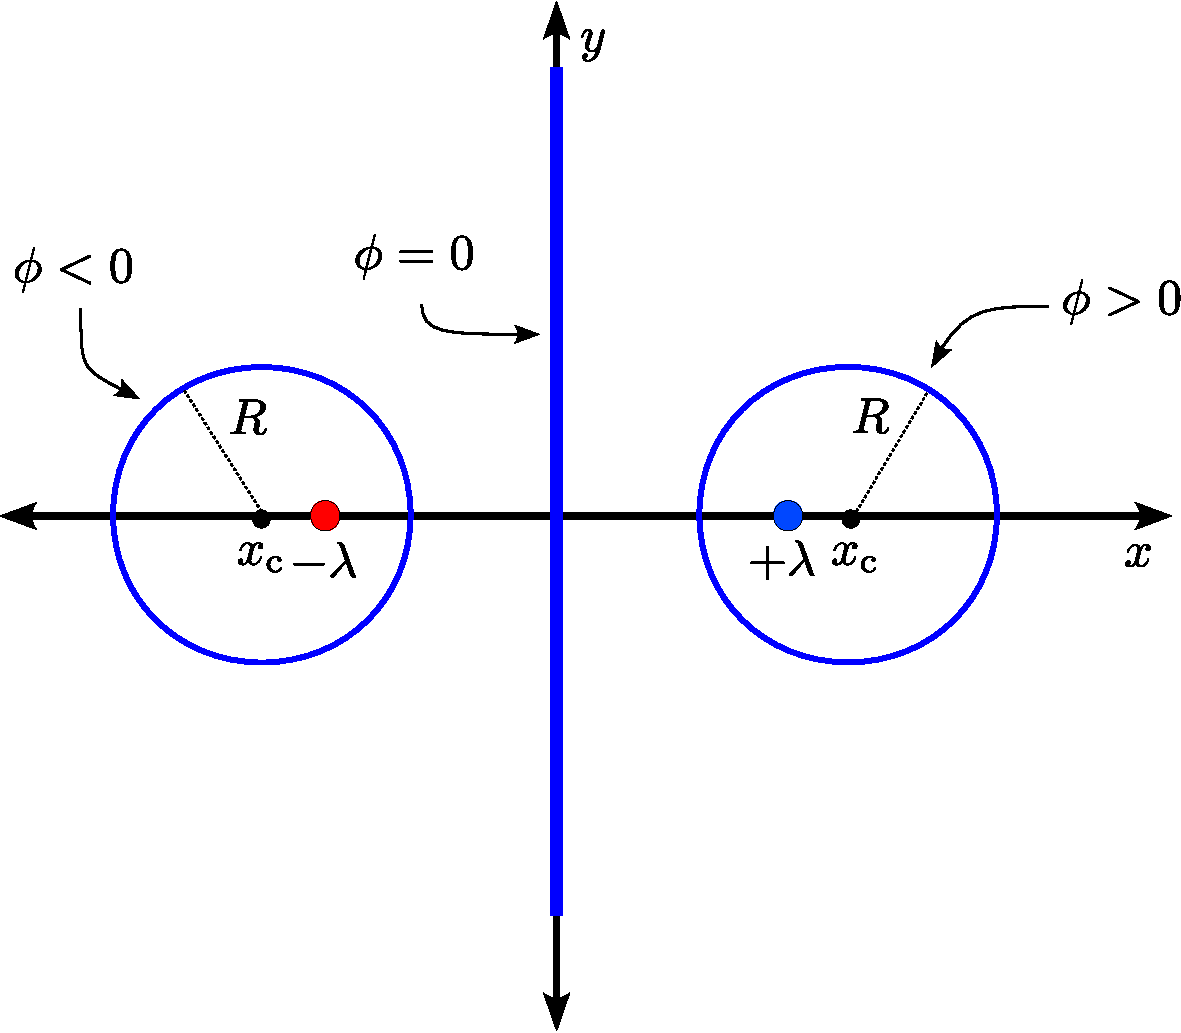
\psfig{file=fig/fig-metodo-imagenes-cilindros-02.pdf,height=6cm,angle=0}
\hspace{1cm}
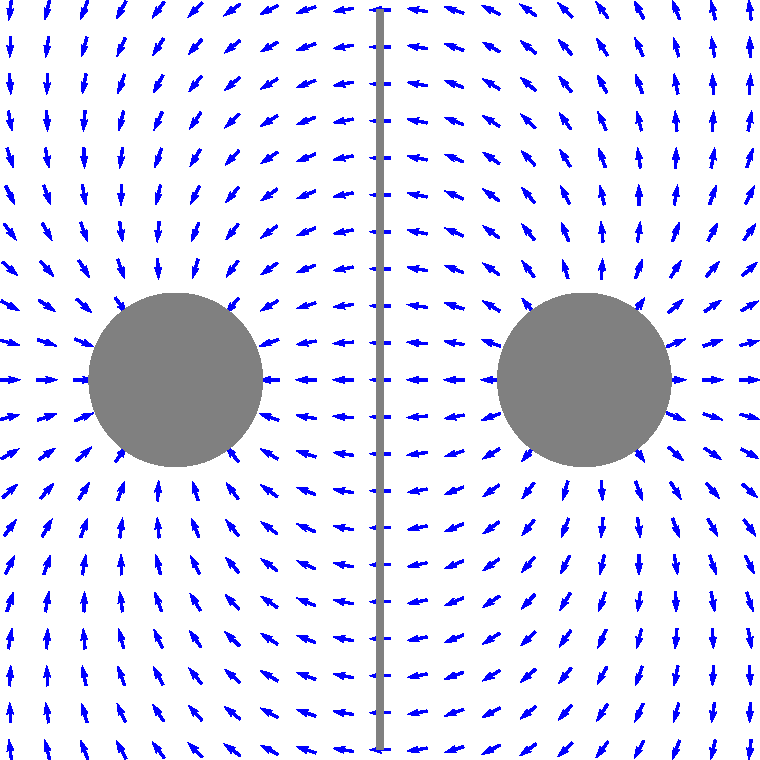
\psfig{file=fig/fig-metodo-imagenes-cilindros-03.pdf,height=6cm,angle=0}}
\caption{Superficies equipotenciales y l'ineas de campo. C'odigo Python de la figura de la derecha disponible \href{https://github.com/gfrubi/electrodinamica/blob/master/figuras-editables/fig-metodo-imagenes-cilindros-03.py}{aqu\'i}.}
\label{ci04}
\end{figure}

\section{Energ'ia potencial el'ectrica de cargas en un campo externo}
Como consecuencia de (\ref{E=nablaphi}), la fuerza electrost'atica es
\textit{conservativa}, pues puede derivarse de una energ'ia potencial (o,
equivalentemente, el trabajo es independiente de la trayectoria, ya que el campo
el'ectrico es irrotacional):
\begin{equation}
\boxed{F_i=qE_i=-q\partial_i\phi .}
\end{equation}
Definimos la \textbf{energ\'{\i}a potencial el'ectrica} de una carga $q$ ubicada en un punto $x$ con campo el'ectrico (externo) descrito por el potencial $\phi(x)$ por
\begin{equation}
\boxed{U(x):=q\phi(x),} \label{Uqphi}
\end{equation}
de modo
que
\begin{equation}
\boxed{F_i(x)=-(\partial_iU)(x) .}
\end{equation}
Como toda energ'ia potencial, la energ'ia potencial el'ectrica es una
cantidad bien definida salvo una constante aditiva arbitraria. Como
consecuencia, \textit{s'olo las diferencias de energ'ia potencial tienen
significado f'isico inambiguo} (pueden en principio ser medidas). Esta caracter'istica se
ilustra m'as claramente si consideramos el trabajo realizado por un campo
el'ectrico sobre una carga $q$ al desplazarse 'esta desde el punto $A$ hasta el
punto $B$:
\begin{equation}\label{WABDU}
W_{A\rightarrow B}=\int_A^B F_i\, dx_i=-\int_A^B
\partial_iU\,dx_i=-\left.U\right|_A^B=-\Delta U=-q\Delta\phi=-q(\phi_B-\phi_A).
\end{equation}

Como consecuencia, una part'icula cargada de masa $m$ y carga $q$ movi'endose en el campo el'ectrico externo descrito por el potencial $\phi$ tendr'a una energ'ia mec'anica $E=K+U=m\vec{v}^2/2+q\phi$, que ser'a constante si no existen otras fuerzas actuando, es decir,
\begin{equation}
E=\frac{1}{2}m\vec{v}^2+q\phi(x)=\text{cte.}
\end{equation}

Podemos generalizar la expresi'on \eqref{Uqphi} para el caso de una distribuci'on cont'inua de cargas \textit{de prueba}, en un campo \textit{externo}. En otras palabras, \textit{despreciamos el campo que las mismas cargas producen}. Por simple superposici'on encontramos que la energ'ia potencial de una distribuci'on de cargas descritas por la densidad $\rho(\vec{x})$ en un campo \textit{externo} $\phi(\vec{x})$ es dado por
\begin{equation} \label{Urhophiext}
U=\int \rho(\vec{x})\,\phi(\vec{x})\,dV.
\end{equation}

%\subsection{Ejemplo}
\section{Energ'ia potencial de un sistema de cargas}  \label{ed3_1}

\subsection{Energ'ia potencial de un conjunto de cargas puntuales}
\label{ed3_1_1}

Consideremos ahora el problema de determinar la \textit{energ'ia potencial total de un
conjunto de $N$ cargas puntuales}, pero \textit{ahora tomando en cuenta el campo que ellas mismas generan}. Cada carga $q^{(\alpha)}$ posee una energ'ia
potencial $U^{(\alpha\beta)}$ asociada al campo el'ectrico producido por cada una de las \textit{otras cargas}  $q^{(\beta)}$, con $\beta\ne \alpha$. Aqu'i $\alpha,\beta=1,\cdots, N$.

Adem'as, el potencial el'ectrico en el punto $\vec{x}$, generado por la carga $q^{(\beta)}$
ubicada en el punto $\vec{x}^{(\beta)}$, es dado por
\begin{equation}
\phi^{(\beta)}(\vec{x})=\frac{1}{4\pi\varepsilon_0}\,\frac{q^{(\beta)}}{|\vec{x}
-\vec{x}^{(\beta)}|} ,
\end{equation}
de modo que
\begin{equation} \label{eq3.1.3}
U^{(\alpha\beta)}=q^{(\alpha)}\,\phi^{(\beta)}(\vec{x}^{(\beta)})=\frac{1}{4\pi\varepsilon_0}\,\frac{q^{(\alpha)}\,q^{(\beta)}}{|\vec{x}^{(\alpha)}-\vec{x}^{(\beta)}|}.
\end{equation}
Vemos de (\ref{eq3.1.3}) que $U^{(\alpha\beta)}=U^{(\beta\alpha)}$, es decir, la energ'ia potencial de la carga $\alpha$-'esima debido al campo producido por la carga
$\beta$-'esima es igual a la energ'ia potencial de la $\beta$-'esima debido al campo
de la $\alpha$-'esima.

Adem'as,  $U^{(\alpha\beta)}\to 0$, cuando  $|\vec{x}^{(\alpha)}|\to\infty$
'o $|\vec{x}^{(\beta)}|\to\infty$. Entonces, de acuerdo a \eqref{WABDU}, \textit{podemos interpretar $U^{(\alpha\beta)}$ como la energ'ia (trabajo) que se necesita para traer la carga
$q^{(\alpha)}$ desde el infinito hasta la posici'on $\vec{x}^{(\alpha)}$, en el campo
el'ectrico producido por la carga $q^{(\beta)}$, fija en $\vec{x}^{(\beta)}$}, o
vicecersa.

Para calcular la energ'ia potencial el'ectrica total de un sistema de muchas cargas
puntuales, ``construimos'' el sistema, carga por carga, tray'endolas desde el
infinito (donde la interacci'on mutua es despreciable): Primero consideramos que la carga $q^{(1)}$ es transportada desde
el infinito hasta su posici'on final $\vec{x}^{(1)}$. Para esto no se requiere
trabajo alguno ya que no existe campo el'ectrico preexistente que act'ue sobre
esta carga. Como segundo paso, traemos la carga $q^{(2)}$ desde el infinito
hasta su posici'on final $\vec{x}^{(2)}$. Este proceso requiere una energ'ia
dada por $U^{(21)}$. En el siguiente paso, traemos $q^{(3)}$ desde el
infinito hasta $\vec{x}^{(3)}$, manteniendo fijas las cargas $q^{(1)}$ y
$q^{(2)}$. La energ'ia requerida para este paso es $U^{(31)}+U^{(32)}$. Hasta
el momento la energ'ia total requerida para formar el sistema de 3 cargas es
$U^{(21)}+U^{(31)}+U^{(32)}=U^{(12)}+U^{(13)}+U^{(23)}$. Continuando
este proceso encontramos que \textit{la energ'ia potencial el'ectrica total de un
sistema de $N$ cargas} $q^{(\alpha)}$, con posiciones $\vec{x}^{(\alpha)}$ es dado por
\begin{equation} \label{eq3.1.4}
U=\sum_{\alpha,\beta\,(\alpha>\beta)}^N U^{(\alpha\beta)}=\frac{1}{4\pi\varepsilon_0}\,
\sum_{\alpha,\beta\,(\alpha>\beta)}^N \frac{q^{(\alpha)}\,q^{(\beta)}}{|\vec{x}^{(\alpha)}-\vec{x}^{(\beta)}|}.
\end{equation}
Alternativamente, ya que $U^{(\alpha\beta)}=U^{(\beta\alpha)}$, podemos escribir
$U=({1}/{2})\sum_{\alpha,\beta\,(\alpha\ne \beta)}^N U^{(\alpha\beta)}$, de modo que
\begin{equation} \label{eq3.1.5}\marginnote{Energ'ia sist. cargas puntuales}
\boxed{U=\frac{1}{8\pi\varepsilon_0}\,
\sum_{\alpha,\beta\,(\alpha\ne \beta)}^N \frac{q^{(\alpha)}\,q^{(\beta)}}{|\vec{x}^{(\alpha)}-\vec{x}^{(\beta)}|}.}
\end{equation}
En t'erminos del \textit{potencial el'ectrost'atico total en el punto $\vec{x}^{(\alpha)}$
debido a todas las otras cargas} $q^{(\beta)}$ ($\beta\ne \alpha$),
\begin{equation}
\phi'(\vec{x}^{(\alpha)})=\frac{1}{4\pi\varepsilon_0}\,
\sum_{\beta\,(\beta\ne \alpha)}^N \frac{q^{(\beta)}}{|\vec{x}^{(\alpha)}-\vec{x}^{(\beta)}|},
\end{equation}
tenemos que
\begin{equation}\label{Wqphi}
\boxed{U= \frac{1}{2}\,\sum_{\alpha=1}^N q^{(\alpha)}\,\phi'(\vec{x}^{(\alpha)}).}
\end{equation}

\subsection{Energ'ia potencial de una distribuci'on continua de cargas} \label{ed3_1_2}
En el caso de una \textit{distribuci'on continua} de carga descrita por una densidad de carga $\rho(\vec{x})$, requerimos una expresi'on similar a la encontrada en la secci'on anterior para cargas puntuales. En el l'imite continuo, esperamos poder reemplazar $q^{(\alpha)}\to dq=\rho(\vec{x})\,dV$. Por otro lado, podr'iamos esperar que el potencial $\phi'(x^{(\alpha)})$ tienda simplemente al potencial de la distribuci'on continua de carga, evaluado en el punto $\vec{x}$, es decir, $\phi'(x^{(\alpha)})\to\phi(\vec{x})$, ya que no tiene sentido hacer distinci'on, en el caso de una distribuci'on continua, entre el campo $\phi'$ (es decir, el potencial producido por las cargas del sistema localizadas en puntos $\vec{x}'\neq\vec{x}$) y el simplemente el potencial $\phi(\vec{x})$. 

De este modo, obtenemos
\begin{equation}\marginnote{Energ'ia de dist. continua}
\boxed{U= \frac{1}{2}\,\int\rho(\vec{x})\,\phi(\vec{x})\,dV.} \label{Urhophi}
\end{equation}

Es importante entender la diferencia entre \eqref{Urhophiext} y \eqref{Urhophi}. La primera expresi'on representa la energ'ia potencial de una distribuci'on de cargas \textit{en un campo externo}, \textit{despreciando el campo que ellas mismas producen} (cargas ``de prueba"), mientras que la segunda representa \textit{la energ'ia potencial total contenida en un sistema de cargas debido su propio campo}. En otras palabras, los potenciales involucrados en \eqref{Urhophiext} y \eqref{Urhophi} son de naturaleza distinta: en la primera expresi'on representa el potencial externo, y en la segunda el potencial generado por las propias cargas. \textit{S'olo en el segundo caso el potencial est'a relacionado con la densidad por medio de la ecuaci'on de Poisson}.

Adem'as, si bien al aplicar la integral \eqref{Urhophi} al caso de distribuciones continuas y finitas de carga se obtienen resultados finitos, al intentar aplicarla al caso de una carga \textit{puntual} (o conjuntos de cargas puntuales) se encuentra un resultado \textit{divergente}. Esto, sin embargo, es usualmente interpretado asumiendo que  una carga puntual es una \textit{idealizaci'on}: el l'imite en que el tama\~no de la carga es nulo.
En la pr'actica, consideraremos a \eqref{Urhophi} como la expresi'on general para la energ'ia de una distribuci'on general de cargas, mientras que para un conjunto de cargas puntuales usaremos (\ref{eq3.1.5}) o, alternativamente, (\ref{Wqphi}).

\subsubsection{Derivaci'on alternativa}
Podemos derivar la expresi'on \eqref{Urhophi} considerando el proceso de ``construcci'on'' del sistema en que la densidad es aumentada paulatinamente desde 0 hasta $\rho(\vec{x})$. Si en un instante dado la densidad es, en cada punto, una fracci'on $\lambda$ ($0\le\lambda\le 0$) de la densidad total, es decir, si la densidad es $\lambda\rho(\vec{x})$, entonces el potencial generado por esta densidad es $\phi_\lambda(\vec{x})=\lambda\phi(\vec{x})$, ya que las la ecuaci'on que determina el potencial a partir de la densidad de carga (la ec. de Poisson (\ref{poisson})) es lineal. Entonces el trabajo necesario para aumentar la fracci'on de carga desde $\lambda$ hasta $\lambda+d\lambda$ es el trabajo necesario para transportar las cargas $dq=d\lambda\,\rho(\vec{x})dV$ desde el infinito hasta sus posiciones finales, en el campo $\phi_\lambda(\vec{x})$. Por lo tanto, el trabajo total requerido para aumentar la densidad de carga en una fracci'on $d\lambda$ es dado por:
\begin{align}
dW &= \int_V dq\,\phi_\lambda(\vec{x}) \\
&= \int_V \left[d\lambda\,\rho(\vec{x})\,dV\right]\left[\lambda\phi(\vec{x})\right] \\
&= \lambda d\lambda\,\int_V \rho(\vec{x})\phi(\vec{x}) \,dV . \label{dWlambda}
\end{align}
La energ'ia requerida en el proceso completo de ``construcci'on'' del sistema de cargas es entonces la suma de los trabajos de la forma (\ref{dWlambda}) desde $\lambda=0$ hasta $\lambda=1$, es decir,
\begin{equation}
U=\int_0^1dW,
\end{equation}
que lleva nuevamente a la expresi'on \eqref{Urhophi}.

\subsubsection{Energ'ia de un sistema de cargas formado por dos subsistemas}
Si tenemos un sistema de cargas que pueda ser separado en dos subsistemas, el primero con densidad de carga $\rho_1(x)$ que genera un potencial $\phi_1(x)$, y el segundo con densidad $\rho_2(x)$ y potencial $\phi_1(x)$, entonces 
\begin{equation}
\rho(x)=\rho_1(x)+\rho_2(x),
\end{equation}
ya suponemos que las regiones donde $\rho_2(x)$ y $\rho_2(x)$ son no nulas son disjuntas. Adem'as, en un punto cualquiera el potencial es dado por
\begin{equation}
\phi(x)=\phi_1(x)+\phi_2(x).
\end{equation}
Reemplazando estas expresiones en nuestro resultado general \eqref{Urhophi} encontramos que  la energ'ia del sistema completo puede ser escrita como
\begin{equation}
U=U_1+U_2+U_{\rm int}
\end{equation}
\begin{equation}
U_1= \frac{1}{2}\,\int\rho_1(\vec{x})\,\phi_1(\vec{x})\,dV ,\qquad U_2= \frac{1}{2}\,\int\rho_2(\vec{x})\,\phi_2(\vec{x})\,dV,
\end{equation}
\begin{align}
U_{\rm int} =& \int \rho_1(x)\phi_2(x)\,dV = \int \rho_2(x)\phi_1(x)\,dV.
\end{align}
La energ'ia $U_{\rm int}$ puede ser interpretada, de acuerdo a nuestro resultado \eqref{Urhophiext}, como la \textbf{energ'ia potencial de las cargas en el subsistema 1 debido al campo (externo) generado por el subsistema 2}, o bien como la \textbf{energ'ia potencial de las cargas en el subsistema 2 debido al campo (externo) generado por el subsistema 1}, o simplemente como la \textbf{energ'ia de interacci'on}.


\subsubsection{Energ'ia en funci'on del campo el'ectrico}

Podemos expresar la energ'ia \eqref{Urhophi} en t'erminos del campo el'ectrico,
usando la ley de Gauss (\ref{leygauss-dif}):
\begin{eqnarray}
U&=&\frac{1}{2}\,\int\rho(\vec{x})\,\phi(\vec{x})\,dV \\
&=&\frac{\varepsilon_0}{2}\,\int(\partial_i E_i)\,\phi\,dV\\
&=&\frac{\varepsilon_0}{2}\,\int\left[
\partial_i(E_i\phi)-E_i\partial_i\phi\right] dV\\
&=&\frac{\varepsilon_0}{2}\left[\oint
E_i\phi\,dS_i-\int E_i\partial_i\phi\, dV\right]\\
&=&\frac{\varepsilon_0}{2}\left[0+\int E_iE_i\, dV\right]\\
&=&\frac{\varepsilon_0}{2}\int \vec{E}^2\, dV.
\end{eqnarray}
En este c'alculo, hemos considerado que la integral de volumen se extiende sobre
todo el espacio, y que el campo el'ectrico se anula suficientemente r'apido en
el infinito, de forma tal que la integral de superficie es nula\footnote{La integral tiende a cero si $\phi$ decae m'as r'apido que $1/\sqrt{r}$ para $r\to\infty$. Esta condici'on es siempre satisfecha para distribuciones compactas de carga, donde se tiene de hecho que $\phi$ decae al menos como $1/r$.}. Con esto,
obtenemos
\begin{equation} \label{UuE}
\boxed{U=\int u_E(\vec{x})\,dV, \qquad u_E(\vec{x}):=\frac{\varepsilon_0}{2}\,
\vec{E}^2(\vec{x}) .}
\end{equation}
De esta forma, podemos calcular la energ'ia (potencial) electrost'atica de una
distribuci'on de carga como la integral de una \textit{densidad de energ'ia}
$u_E(\vec{x})$. Comparando (\ref{UuE}) con (\ref{eq3.1.5}) vemos que la
energ'ia potencial de un sistema de cargas puede interpretarse alternativamente
como la \textit{energ'ia almacenada en el campo el'ectrico} del sistema de
cargas, a trav'es de la densidad de energ'ia $u_E(\vec{x})$.

\subsubsection{Ejemplo}
\begin{figure}[!h]
\centerline{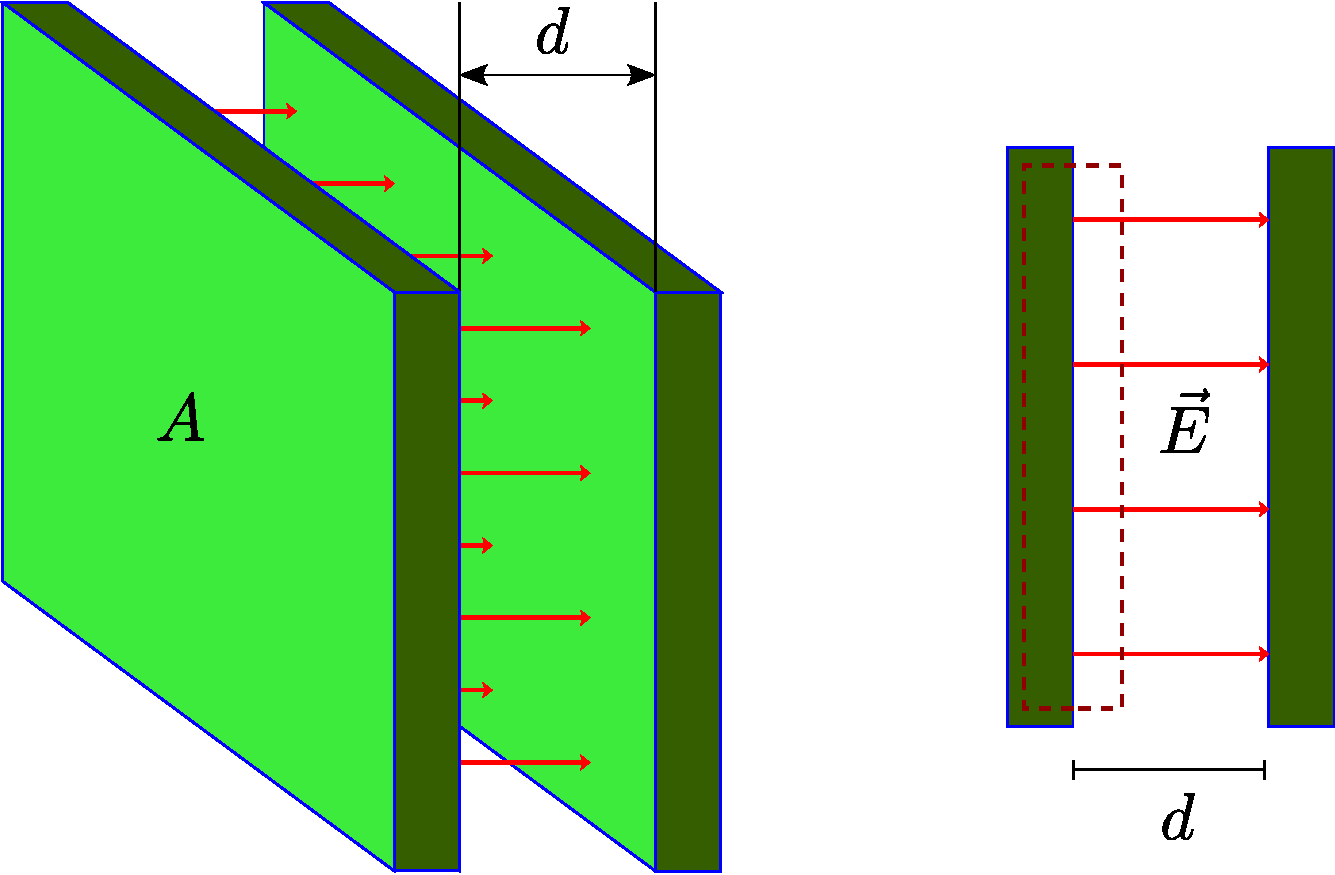
\psfig{file=fig/fig-condensador-01.pdf,height=4cm,
angle=0 } }
\caption{Energ'ia almacenada en un condensador de placas paralelas.}
\label{fig:cpp}
\end{figure}
Considere un condensador de placas paralelas, como se muestra en la figura \ref{fig:cpp}. Despreciando efectos de borde, es decir, considerando que dentro de la regi'on limitada por las placas en campo el'ectrico es homog'eneo y fuera de ella es nulo, y adem'as despreciando el espesor de las placas, podemos modelar la densidad de carga como
\begin{equation}
\rho(\vec{x})=\sigma\delta(x)-\sigma\delta(x-d), 
\end{equation}
para todo $(y,z)$ en la regi'on delimitada por las placas. 

El campo el'ectrico entre las placas (que puede obtenerse f'acilmente usando la ley de Gauss) es dado por
\begin{equation}
\vec{E}=\frac{\sigma}{\varepsilon_0}\hat{x}=E\hat{x}, \qquad 0<x<d,
\end{equation}
donde $\sigma$ es la densidad total de carga por unidad de superficie (en cada placa ubicada en $x=0$). Con esto, podemos evaluar la energ'ia \eqref{UuE} (el campo el'ectrico s'olo es no nulo entre las placas, que encierrar un volumen $V=Ad$):
\begin{equation} 
U=\int u_E(\vec{x})\,dV=\frac{\varepsilon_0}{2}\,
\vec{E}^2 V=\frac{\varepsilon_0}{2}\,
\vec{E}^2 Ad=\frac{\sigma^2}{2\varepsilon_0}Ad=\frac{Q^2}{2\varepsilon_0}\frac{d}{A} .
\end{equation}

Por otro lado, usando \eqref{phiintE} encontramos que el potencial entre las placas es de la forma
\begin{equation}
\phi(\vec{x})=\phi(0)-Ex=\phi(0)-\frac{\sigma}{\varepsilon_0}x, \qquad 0<x<d,
\end{equation}
con lo que podemos evaluar \eqref{Urhophi} (la densidad de carga s'olo es no nula sobre las placas), obteniendo
\begin{equation}
U=\frac{1}{2}\int\rho(x)\phi(x)\,dV=\frac{1}{2}\left[\sigma A\phi(0)-\sigma A\phi(d)\right]=\frac{\sigma^2 Ad}{2\varepsilon_0}=\frac{Q^2}{2\varepsilon_0}\frac{d}{A}.
\end{equation}
En t'erminos de la \textit{capacidad del condensador}, $C:=Q/\Delta V=\varepsilon_0 A/d$, tenemos
\begin{equation}
U=\frac{C(\Delta V)^2}{2}=\frac{Q^2}{2C}.
\end{equation}





\section{Expansi'on multipolar cartesiana}
\subsection{Expansi'on Multipolar}
\begin{figure}[!h]
\centerline{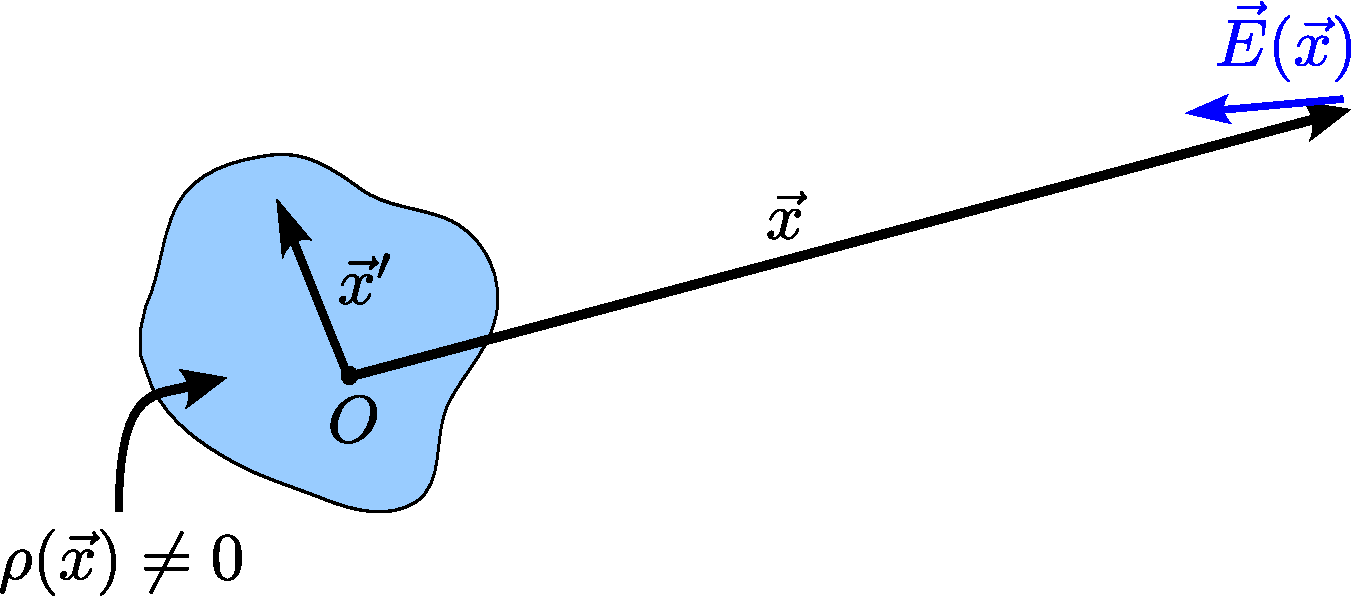
\psfig{file=fig/fig-expansion-multipolar-electrica-01.pdf,height=4cm,
angle=0 } }
\caption{Esquema de la expansi'on multipolar el'ectrica.}
\label{fig:emc}
\end{figure}
El m'etodo de {\em expansi'on multipolar} permite calcular los campos (potencial y campo el'ectrico) de una
\textit{distribuci'on compacta, pero arbitraria}, de carga en forma relativamente sencilla y general. Consideramos entonces una distribuci'on compacta de carga, situaremos (sin p'erdida de generalidad) el origen del sistema coordenado en un punto representativo de la distribuci'on (no necesariamente el centro de masa o el centro de carga), y consideraremos el problema de describir el
campo generado por esta distribuci'on en puntos muy alejados de ella, de modo
que $|\vec{x}|\gg|\vec{x}'|$, ver figura \ref{fig:emc}. Esto permite
reescribir la expresi'on general (\ref{perho}) para el potencial
el'ectrico, en forma de una expansi'on en serie, ya
que el t'ermino $1/\left|\vec{x}-\vec{x}'\right|$ puede ser expandido\footnote{Para esto usamos la expresi'on general para una expansi'on en serie de Taylor de una funci'on de varias variables: $f(x_i+x'_i)=f(x_i)+x'_i\left.(\partial_if)\right|_x+(1/2!)\,x'_ix'_j\left.(\partial_i\partial_jf)\right|_x +(1/3!)\,x'_ix'_jx'_k\left.(\partial_i\partial_j\partial_kf)\right|_x+\dots$.}
en potencias de las componentes del vector $\vec{x}'$:
\begin{eqnarray}
\frac{1}{\left|\vec{x}-\vec{x}'\right|}
%&=&\frac{1}{\left|\vec{x}\right|}
%+x'_i\partial'_i\left(\frac{1}{\left|\vec{x}-\vec{x}'\right|} \right)
%_{x'_i=0}+\frac{1}{2!}x'_ix'_j\,\partial'_i\partial'_j\left(\frac{1}{\left|\vec{
%x } -\vec{x}'\right|} \right) _{x'_i=0}+\dots \\
&=&\frac{1}{\left|\vec{x}\right|}
-x'_i\partial_i\left(\frac{1}{\left|\vec{x}-\vec{x}'\right|} \right)
_{x'_i=0}+\dots+(-1)^2\frac{1}{2!}x'_ix'_j\,
\partial_i\partial_j\left(\frac{1} { \left|\vec{x}-\vec{x}
'\right|} \right) _{x'_i=0}+\dots \\
&=&\frac{1}{\left|\vec{x}\right|}-x'_i\partial_i\frac{1}{\left|\vec{x}\right|}
 +\frac{(-1)^2}{2!}x'_ix'_j\,\partial_i\partial_j\frac{1}{\left|\vec{x}\right|}
+\dots \\
&=&\frac{1}{r}-x'_i\partial_i\frac{1}{r}+\frac{(-1)^2}{2!}x'_ix'_j\,
\partial_i\partial_j\frac{1}{r} +\dots \\
&=&\sum_{n=0}^\infty\frac{(-1)^n}{n!}x'_{i_1}\dots x'_{i_n}\partial_{i_1}\dots
\partial_{i_n}\frac{1}{r} .\label{exp1or}
\end{eqnarray}
Note que los t'erminos con derivadas de la forma $\partial_{i_1}\cdots
\partial_{i_n}r^{-1}$ son funciones (relativamente) simples y \textit{conocidas}.
Por ejemplo:
\begin{eqnarray}
\partial_i\frac{1}{r}&=&-\frac{x_i}{r^3}, \\
\partial_i\partial_j\frac{1}{r}
&=& \frac{3x_ix_j}{r^5}-\frac{\delta_{ij}}{r^3} \\
\partial_i\partial_j\partial_k\frac{1}{r}
&=& \frac{3\left(x_i\delta_{jk}+x_j\delta_{ki}+x_k\delta_{ij}\right)}{r^5}
-\frac{15x_ix_jx_k}{r^7},
\end{eqnarray}
etc. Con esto, podemos escribir
\begin{equation} \label{eq3.2.3}
\frac{1}{|\vec{x}-\vec{x}'|}=\frac{1}{r}+\frac{x_ix'_i}{r^3}
+\frac{1}{2}\,x'_ix'_j\,\left(\frac{3x_ix_j}{r^5}-\frac{\delta_{ij}}{
r^3}\right)+O\left(x_i'^3\right).
\end{equation}
En general, el t'ermino de orden $n$, $\partial_{i_1}\cdots
\partial_{i_n}r^{-1}$, decrecer'a con la distancia como $r^{-(n+1)}$.

Con la expansi'on (\ref{exp1or}) podemos reescribir la expresi'on
(\ref{perho}) para un potencial electrost'atico general (imponiendo $\phi=0$ en el infinito) como
\begin{eqnarray}
\phi(\vec x)&=&\frac{1}{4\pi\varepsilon_0}\int_V\frac{\rho(\vec x')}{
\left\vert \vec x-\vec x'\right\vert }dV'\\
&=&\frac{1}{4\pi\varepsilon_0}\int_V \rho(\vec
x')\sum_{n=0}^\infty\frac{(-1)^n}{n!}x'_{i_1}\dots x'_{i_n}\partial_{i_1}\cdots
\partial_{i_n}\frac{1}{r}dV'\\
&=&\frac{1}{4\pi\varepsilon_0}\sum_{n=0}^\infty\frac{(-1)^n}{n!}\left[\int_V
\rho(\vec x')\,x'_{i_1}\dots x'_{i_n}\,dV'\right]\partial_{i_1}\cdots
\partial_{i_n}\frac{1}{r}. \label{phimult}
\end{eqnarray}
Definiendo el momento multipolar de orden $n$ como el tensor de rango $n$ dado
por
\begin{equation}
\boxed{Q_{i_1\cdots i_n}:=\int_V \rho(\vec x)\,x_{i_1}\dots x_{i_n}\,dV,}
\end{equation}
podemos expresar un campo el'ectrost'atico general por medio de la
\textit{expansi'on multipolar}
\begin{equation}
 \boxed{\phi(\vec
x)=\frac{1}{4\pi\varepsilon_0}\sum_{n=0}^\infty\frac{(-1)^n}{n!}\,Q_{ i_1\cdots
i_n}\,\partial_{i_1}\cdots\partial_{i_n}\frac{1}{r}.} \label{phimult2}
\end{equation}
En otras palabras, podemos descomponer el potencial electrost'atico en una suma
de t'erminos de distinto orden en la expansi'on multipolar
\begin{equation}
 \boxed{\phi(\vec{x})=\sum_{n=0}^\infty\phi^{(n)}(\vec{x}),}
\end{equation}
donde $\phi^{(n)}(\vec{x})$ es la contribuci'on multipolar de orden $n$,
definida por
\begin{equation}
\boxed{\phi^{(n)}(\vec{x}):=\frac{1}{4\pi\varepsilon_0}\,\frac{(-1)^n}{n!}\,Q_{
i_1\cdots i_n}\,\partial_{i_1}\cdots\partial_{i_n}\frac{1}{r}.}
\end{equation}
Los primeros t'erminos de esta expansi'on general son de la forma:
\begin{equation} \label{eq3.2.4}
\phi(\vec{x})=\phi^0(\vec{x})+\phi^{(1)}(\vec{x})+\phi^{(2)}(\vec{x})+
\ldots.
\end{equation}
El t'ermino {\em monopolar} es
\begin{equation} \label{eq3.2.5}
\phi^0(\vec{x})=\frac{1}{4\,\pi\varepsilon_0}\,\frac{Q}{r},
\end{equation}
donde $Q$, el \textit{momento monopolar}, es simplemente la carga total del sistema:
\begin{equation} \label{eq3.2.6}
Q=\int \rho(\vec{x})\,dV.
\end{equation}
El segundo t'ermino, el t'ermino {\em dipolar} es dado por
\begin{equation}
\phi^{(1)}(\vec{x}) =\frac{1}{4\,\pi\varepsilon_0}\,\frac{x_i\,p_i}{r^3},
\end{equation}
donde $p_i:=Q_i$ es el \textit{momento dipolar} del sistema:
\begin{equation} \label{eq3.2.8}
p_i:=\int x_i\,\rho(\vec{x})\,dV.
\end{equation}
La tercera contribuci'on viene dada por el t'ermino {\em cuadrupolar}:
\begin{equation} \label{eq3.2.9}
\phi^{(2)}(\vec{x})=\frac{1}{4\,\pi\varepsilon_0}\,\frac{1}{2}\,Q_{ij}
\left(\frac{3\,x_i\,x_j}{r^5}-\frac{\delta_{ij}}{r^3}\right).
\end{equation}
El \textit{momento cuadrupolar} $Q_{ij}$ es dado por
\begin{equation}
Q_{ij}:=\int x_ix_j\,\rho(\vec{x})\,dV. \label{mom4}
\end{equation}
Con esto, la expansi'on multipolar del potencial es de la forma:
\begin{equation} \label{eq3.2.12}
\boxed{\phi(\vec{x})=\frac{1}{4\,\pi\varepsilon_0}\,\frac{Q}{r}+
\frac{1}{4\pi\varepsilon_0}\,\frac{\vec{p}\cdot\vec{x}}{r^3}+
\frac{1}{4\pi\varepsilon_0}\,\frac{1}{2}\,Q_{ij}\left(\frac{3\,x_i\,x_j}{
r^5}-\frac{\delta_{ij}}{r^3}\right)+O(r^{-4})}
\end{equation}
Podemos tambi'en encontrar una expansi'on multipolar para el campo el'ectrico
simplemente derivando el potencial. Con esto, obtenemos
\begin{align} \label{eq3.2.12.1}
E_i(\vec{x}) =& \frac{Q}{4\pi\varepsilon_0}\,\frac{x_i}{r^3}+\frac{1}{
4\pi\varepsilon_0}\,\frac{(3\,p_j\,x_j\,x_i-r^2\,p_i)}{r^5} \nonumber\\
& - \frac{1}{4\pi\varepsilon_0}\frac{1}{2}Q_{jk}\left[
\frac{3\left(x_i\delta_{jk}+x_j\delta_{ki}+x_k\delta_{ij}\right)}{r^5}
-\frac{15x_ix_jx_k}{r^7}\right]
+O(r^{-5}) .
\end{align}

Observaciones:

\begin{itemize} 
\item El momento multipolar de orden $n$, $Q_{i_1\dots i_n}$ es un tensor sim'etrico de rango $n$ respecto a transformaciones ortogonales de coordenadas. Por eso, $Q_{i_1\dots i_n}$ tiene $(n+1)(n+2)/2$ componentes linealmente independientes.

\item Los momentos multipolares son cantidades \textit{aditivas} (o extensivas). Esto quiere decir que si se divide un sistema en dos partes (el volumen donde est'an contenidas las cargas, en dos volumenes m'as peque\~nos o, equivalentemente, la densidad de carga en la suma de dos densidades) entonces cada momento multipolar (de un orden dado) es la suma de los momentos multipolares de cada subsistema.

\item Note que los momentos multipolares \textbf{dependen en general de la
elecci'on del origen}. Si se desplaza el origen del sistema coordenado de modo que el origen $O$ original tenga coordenadas $\vec{d}$ respecto al nuevo origen $O'$ entonces
$\vec{x}'=\vec{x}+\vec{d}$ y los nuevos momentos multipolares respecto al origen $O'$ est'an dados por:
\begin{eqnarray}
 Q'&=&Q,\\
Q'_i&=&Q_i+Qd_i,\\
Q'_{ij}&=&Q_{ij}+Q_id_j+Q_jd_i+Qd_id_j,
\end{eqnarray}
etc.
\end{itemize}

\subsubsection{Momento cuadrupolar sin traza}\label{MCSM}
El momento cuadrupolar (\ref{mom4}) es un tensor \textit{sim'etrico}, por lo
que tiene ${3\cdot (3+1)}/{2}=6$ componentes linealmente independientes (que
hay que calcular!). Sin embargo, debido a que este tensor siempre est'a
multiplicado en la expansi'on multipolar del potencial por
$\left({3\,x_i\,x_j}/{r^5}-{\delta_{ij}}/{r^3}\right)$, puede
verificarse que no todas las componentes de $Q_{ij}$ contribuyen a la
expansi'on multipolar. En efecto, debido a que la contracci'on
$\delta_{ij}\left({3\,x_i\,x_j}/{r^5}-{\delta_{ij}}/{r^3}\right)$ se
anula \textit{id'enticamente}, es posible sumar un t'ermino proporcional a
$\delta_{ij}$ al momento cuadrupolar, sin por ello alterar la expansi'on
multipolar. En otras palabras, existe una libertad para redefinir el momento
cuadrupolar ya que $\tilde{Q}_{ij}:=Q_{ij}+\lambda\delta_{ij}$ puede ser
considerado como un momento cuadrupolar 'util y leg'itimo. 

Una posibilidad ser'ia elegir $\lambda\stackrel{!}{=}-Q_{ii}$, en cuyo caso obtendr'iamos
\begin{equation}
 \boxed{Q'_{ij}=\int
(x_ix_j-x_kx_k\delta_{ij})\,\rho(\vec{x})\,dV,}
\end{equation}
que, salvo un signo global, tiene la misma forma que el conocido tensor momento de inercia asociado a un cuerpo en rotaci'on. En este sentido, el momento cuadrupolar el'ectrico es el an'alogo al tensor momento de inercia en mec'anica.

Sin embargo, es m'as com'un explotar la libertad para elegir $\lambda$ para definir el  \textit{momento cuadrupolar libre de traza}, definido tal que $\tilde{Q}_{ii}\equiv 0$. Esto equivale a considerar $\lambda\stackrel{!}{=}-Q_{ii}/3$, es decir, $\tilde{Q}_{ij}=Q_{ij}-Q_{kk}\,\delta_{ij}/3$ o,
m'as expl'icitamente:
\begin{equation}
 \boxed{\tilde{Q}_{ij}=\int
(x_ix_j-\frac{1}{3}x_kx_k\delta_{ij})\,\rho(\vec{x})\,dV.} \label{mom4st}
\end{equation}
La ventaja de usar este tensor es que, por ser libre de traza, s'olo tiene 5
componentes linealmente independientes (que calcular, por ejemplo:
$\tilde{Q}_{11}$, $\tilde{Q}_{12}$, $\tilde{Q}_{13}$, $\tilde{Q}_{22}$,
$\tilde{Q}_{23}$, ya que $\tilde{Q}_{21}=\tilde{Q}_{12}$,
$\tilde{Q}_{31}=\tilde{Q}_{13}$, $\tilde{Q}_{32}=\tilde{Q}_{23}$ y
$\tilde{Q}_{33}=-\tilde{Q}_{11}-\tilde{Q}_{22}$) (pero, por otro lado, la integral que se necesita calcular es algo m'as complicada).

Adem'as, el momento cuadrupolar (con o sin traza), por ser un tensor \textit{sim'etrico} de segundo rango, puede ser diagonalizado, es decir, es posible encontrar sus vectores (y valores) propios, que definen direcciones ``principales'', ortogonales entre si. En el sistema coordenado definido por estas tres direcciones principales el momento cuadrupolar adopta una forma diagonal.


\subsubsection{Monopolo ideal}
Una carga puntual es un ``monopolo ideal"\,, ya que (eligiendo el origen en la posici'on de la carga) el 'unico momento distinto de cero es el momento monopolar. 

\subsubsection{Dipolo ideal}
Un ``dipolo ideal"\,(tambi'en llamado ``dipolo puntual'') es un sistema idealizado cuyo 'unico momento multipolar el'ectrico no nulo es el momento dipolar.

El sistema formado por una carga $q^{(1)}=-q$ y otra $q^{(2)}=+q$, separados una distancia $d$ tiene momento monopolar nulo, mientras que 
\begin{equation}
p_i=(-q)x^{(1)}_i+(+q)x^{(2)}_i=q(x^{(2)}_i-x^{(1)}_i)=qd_i,
\end{equation}
\begin{equation}
Q_{ij}=(-q)x^{(1)}_i x^{(1)}_j +(q)x^{(2)}_i x^{(2)}_j,
\end{equation}
\begin{equation}
Q_{ijk}=(-q)x^{(1)}_i x^{(1)}_jx^{(1)}_k +(q)x^{(2)}_i x^{(2)}_jx^{(2)}_k,
\end{equation}
etc. En el l'imite $\vec{d}\to\vec{0}$, pero tal que $\vec{p}$ sea finito (esto, por supuesto, requiere $q\to\infty$), tendremos que $Q_{ij}\to 0$, $Q_{ijk}\to 0$, y lo mismo ocurrir'a para todo momento multipolar de orden superior  (las componentes del momento multipolar de orden $n$ son en este caso proporcionales a $qd^n=pd^{n-1}$).

\begin{equation}\label{phip}
\phi_{\vec{p}}(\vec{x})=\frac{1}{4\pi\varepsilon_0}\frac{(x_j-x_j')p_j}
{|\vec{x}-\vec{x}'|^3},
\end{equation}
\begin{figure}[H]
\begin{center}
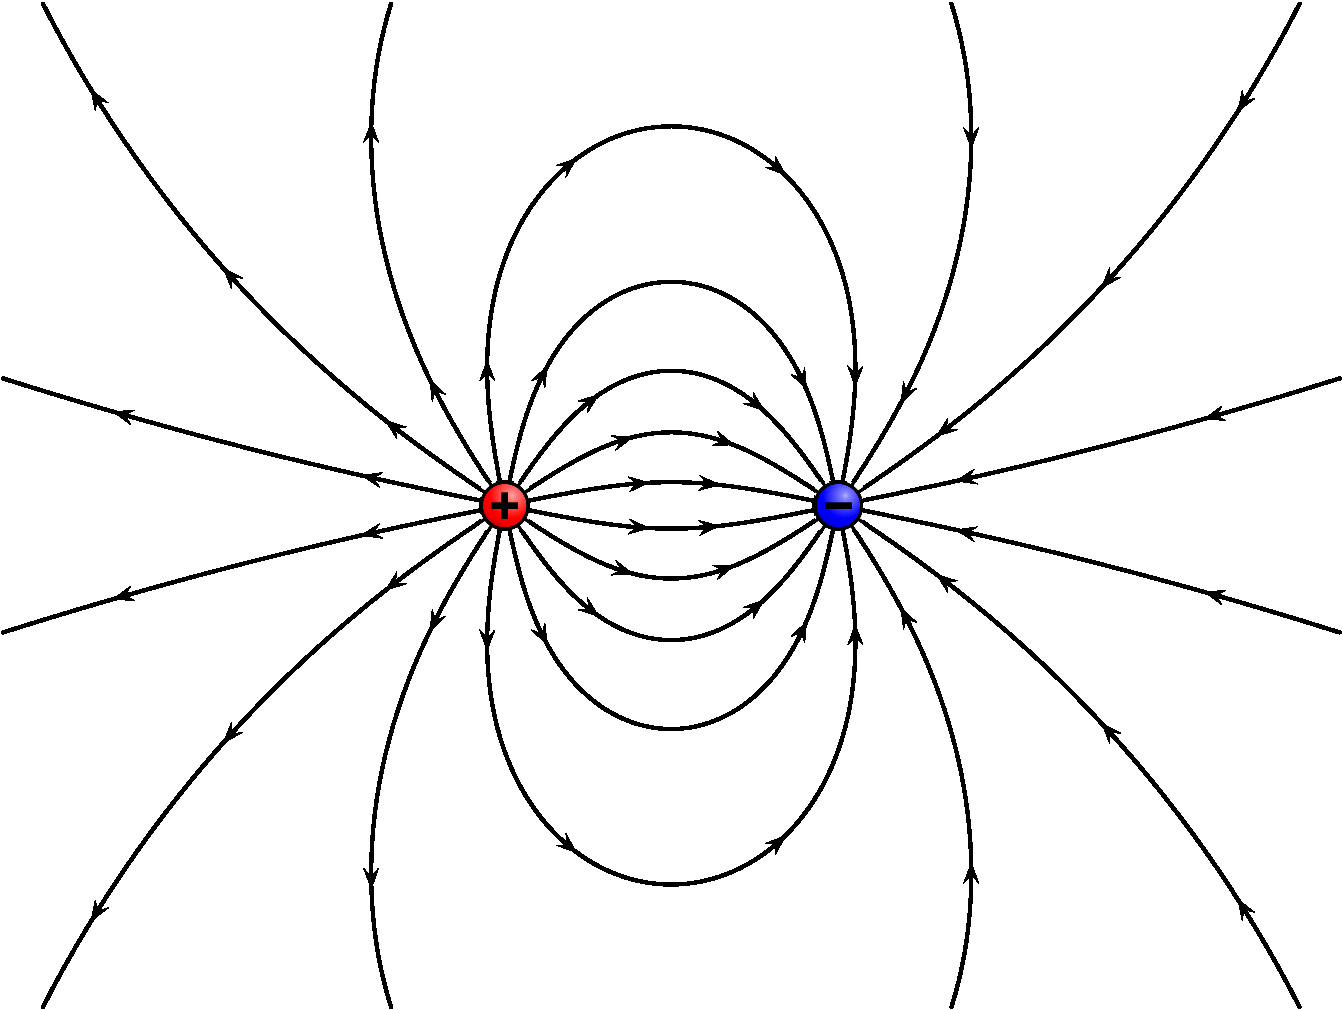
\includegraphics[height=4cm]{fig/fig-E-02.pdf}\hspace{1cm}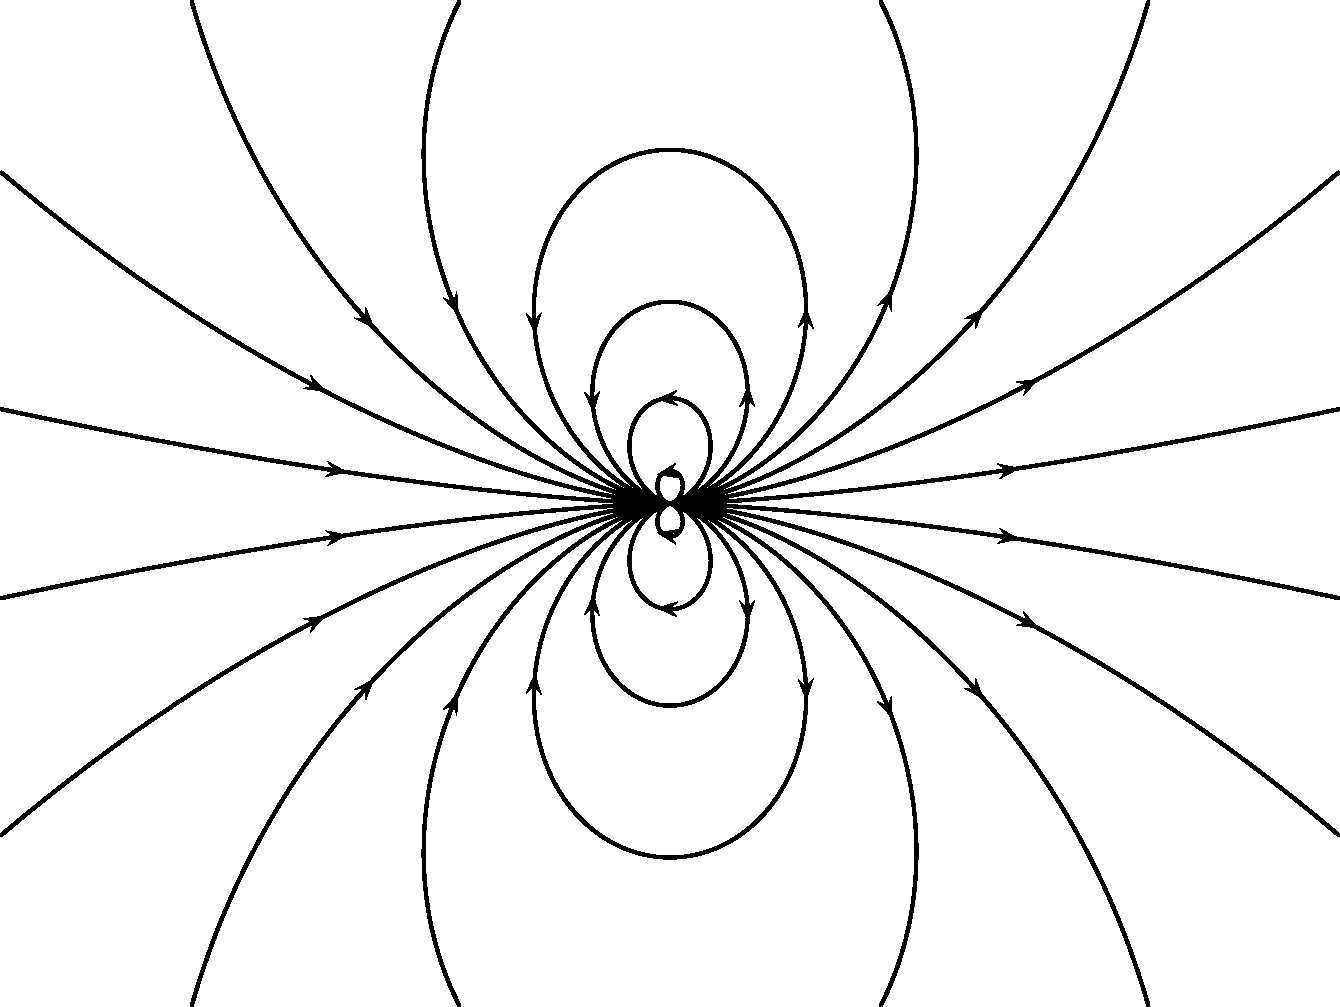
\includegraphics[height=4cm]{fig/fig-campo-dipolo-electrico.pdf} 
\caption{Dipolo (dos cargas opuestas) versus dipolo ideal. Figuras creadas usando VectorFieldPlot \cite{VFP}.}
\label{fig-dipolos}
\end{center}
\end{figure}
\subsubsection{Cuadrupolo ideal}
$Q=0$ $p_i=0$, $Q_{ij}\neq 0$, $Q_{ijk}=0$, etc.

\begin{figure}[H]
\begin{center}
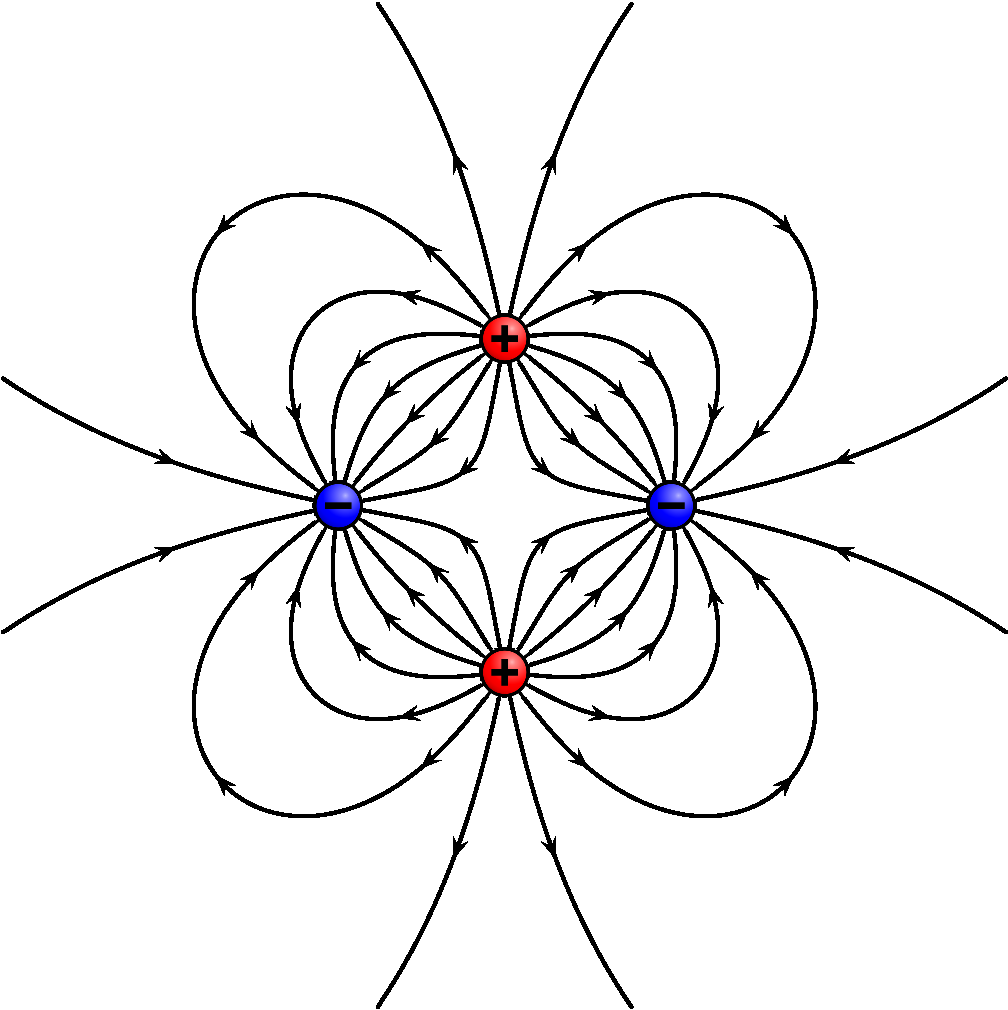
\includegraphics[height=4cm]{fig/fig-E-03.pdf}\hspace{1cm}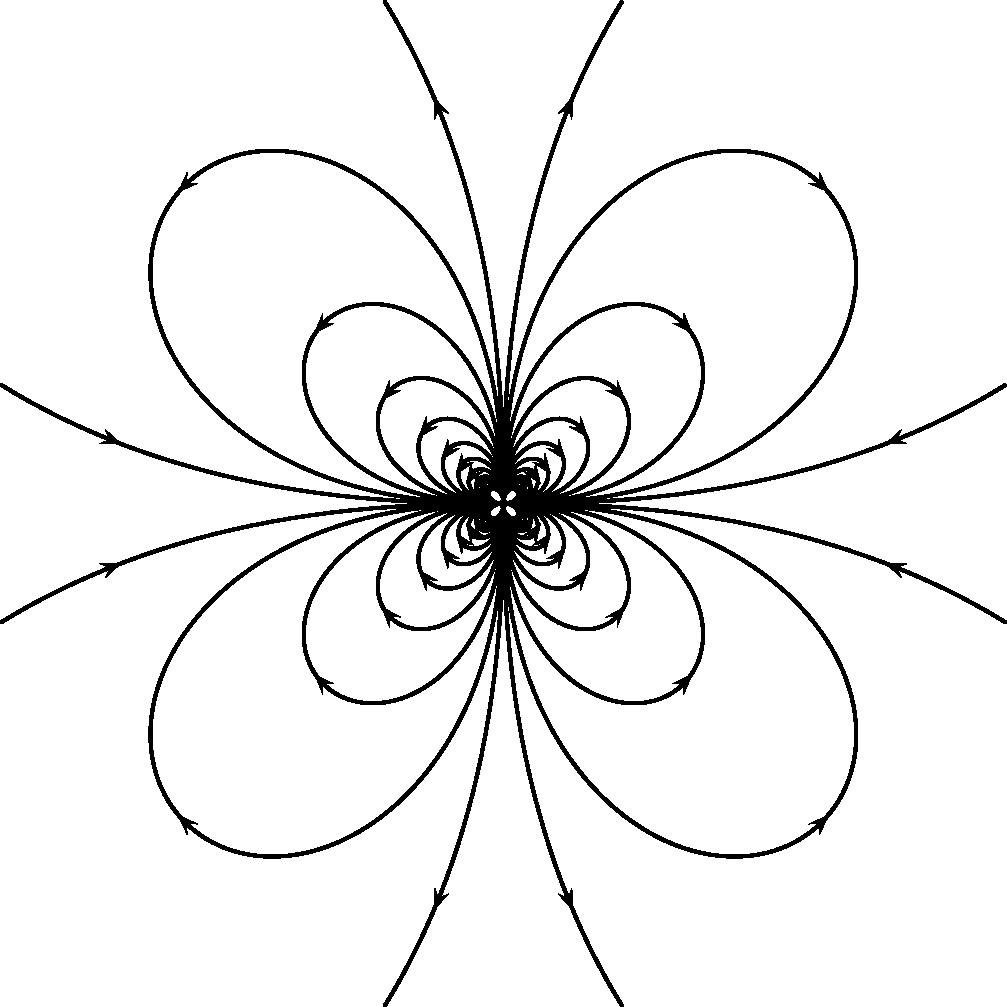
\includegraphics[height=4cm]{fig/fig-campo-cuadrupolo-electrico-ideal.pdf} 
\caption{Cuadrupolo versus cuadrupolo ideal. Figuras creadas usando VectorFieldPlot \cite{VFP}.}
\label{fig-dipolos}
\end{center}
\end{figure}
\newpage


\subsection{Distribuciones de carga en campos externos} \label{ed3_3}

En las secciones anteriores hemos considerado la expansi'on multipolar
\textit{generada} por una distribuci'on compacta de carga
$\rho(\vec{x})$. Ahora discutiremos una situaci'on distinta: consideraremos
una (peque\~na) distribuci'on de cargas en un campo el'ectrico
\textit{externo} (es decir, generado por alguna \textit{otra} distribuci'on de
carga). En particular, calcularemos la energ'ia potencial de la
distribuci'on de carga en el campo externo dado, as'i como la fuerza y el
torque que el campo externo ejerce.

\subsubsection{Energ'ia Potencial} \label{ed3_3_1}


Para evaluar esta integral, consideramos un \textit{punto representativo $P$ de la
distribuci'on} con coordenadas $\vec{x}$ y un punto $P'$ cualquiera de la
distribuci'on  (con coordenadas $\vec{x}+\vec{x}'$ respecto
al origen, ver figura) determinado por el vector $\vec{x}'$ respecto al punto
representativo $P$ de la distribuci'on, y expandiremos los valores $\phi(P')$ en
una serie de Taylor en torno a $P$:
\begin{align} \label{eq3.3.3}
\phi(P') = &\ \phi(\vec{x}+\vec{x}')\\
= & \sum_{n=0}^\infty\frac{1}{n!}x'_{i_1}\cdots
x'_{i_n}\left.(\partial_{i_1}\cdots\partial_{i_n}\phi)\right|_{\vec{x}'=\vec{0}} \\
= &\ \left.\phi\right|_{\vec{x}'=\vec{0}}+x'_i\left.(\partial_i\phi)\right|_{\vec{
x}'=\vec{0}}+\frac{1}{2}x'_ix'_j\left.(\partial_i\partial_j\phi)\right|_{\vec{x}
'=\vec{0}}+\cdots \nonumber\\
& +\frac{1}{n!}x'_{i_1}\cdots
x'_{i_n}\left.(\partial_{i_1}\cdots\partial_{i_n}\phi)\right|_{\vec{x}'=\vec{0}}
+\cdots\\
= &\ \phi(\vec{x})-x'_iE_i(\vec{x})-\frac{1}{2}x'_ix'_j(\partial_iE_j)(\vec{x}
) \nonumber \\
& -\cdots-\frac{1}{n!}x'_{i_1}\cdots
x'_{i_n}(\partial_{i_1}\cdots\partial_{i_{n-1}}E_{i_n})(\vec{x})+\cdots .
\end{align}

Con esto, podemos escribir (\ref{Urhophiext}) como
\begin{eqnarray}
 U&=&\int\rho(P')\,\phi(P')\,dV'\\
&=&\sum_{n=0}^\infty\frac{1}{n!}\left[\int\rho(P')x'_{i_1}\cdots
x'_{i_n}\,dV'\right]\left.(\partial_{i_1}\cdots\partial_{i_n}\phi)\right|_{\vec{x}'=\vec{0}}\\
%&=&\left[\int\rho(\vec{x}')
%\phi(\vec{x})-\left[\int\rho(\vec{x}')\,
%x'_i\,dV'\right] E_i(\vec{x})-\frac{1}{2}\left[ \int\rho(\vec{x}')\,
%x'_ix'_j\,dV'\right](\partial_iE_j)(\vec{x})
%\nonumber\\
%&&-\cdots-\frac{1}{n!}\left[ \int\rho(\vec{x }')\, x'_{i_1}\cdots
%x'_{i_n}\,dV'\right] (\partial_{i_1}
%\cdots\partial_{i_{n-1}}E_{i_n})(\vec{x})+\cdots \\
&=&\sum_{n=0}^\infty\frac{1}{n!}Q_{i_1\cdots i_n}(\partial_{i_1}\cdots\partial_{i_n}\phi)(\vec{x})\\
&=&Q\phi(\vec{x})-Q_iE_i(\vec{x})-\frac{1}{2}
Q_{ij}(\partial_iE_j)(\vec{x}) \nonumber \\
&& -\cdots-\frac{1}{n!}Q_{i_1\cdots i_n}(\partial_{i_1}
\cdots\partial_{i_{n-1}}E_{i_n})(\vec{x})+\cdots .
\end{eqnarray}
Por lo tanto, obtenemos que la energ'ia potencial de una distribuci'on de
carga, caracterizada por sus momentos multipolares, en un \textit{campo externo}
es dado por
\begin{equation} \label{eq3.3.4}
\boxed{U=Q\,\phi(\vec{x})-\vec{p}\cdot\vec{E}(\vec{x})-\frac{1}{2}\,Q_{ij}
\,\partial_iE_j(\vec{x})+\cdots .}
\end{equation}

El primer t'ermino de esta expansi'on, la contribuci'on monopolar, es
equivalente a la de una carga \textit{puntual} en un potencial externo. El
t'ermino siguiente (dipolar) representa la energ'ia potencial de un dipolo
ideal en un campo el'ectrico externo. Note que este t'ermino es m'inimo cuando
el momento dipolar es paralelo al campo el'ectrico externo (y es, en general,
proporcional al coseno del 'angulo entre $\vec{p}$ y $\vec{E}$). El t'ermino
cuadrupolar es distinto de cero s'olo cuando el campo es inhomog'eneo. Note que
en esta expresi'on tambi'en es posible usar un momento cuadrupolar redefinido
como se discuti'o en la secci'on (\ref{MCSM}). En particular puede usarse el
momento cuadrupolar sin traza. La energ'ia potencial calculada usando distintos
momentos cuadrupolares equivalentes es la misma puesto que un t'ermino
proporcional a $\delta_{ij}$ contribuira con un t'ermino proporcional a
$\delta_{ij}(\partial_iE_j)=\partial_iE_i$, que es cero en virtud de la ley de
Gauss y el hecho que $\vec{E}$ describe un \textit{campo el'ectrico externo},
es decir, un campo generados por fuentes fuera de la regi'on bajo
consideraci'on.


\subsubsection{Fuerza}  \label{ed3_3_2}

Una carga puntual $q$ experimenta una fuerza
$\vec{F}(\vec{x})=q\,\vec{E}(\vec{x})$ cuando est'a situada en
un punto donde existe un campo externo $\vec{E}(\vec{x})$. Como consecuencia,
la fuerza total sobre una distribuci'on con densidad $\rho$ en un campo
\textit{externo} puede escribirse como
\begin{equation} \label{eq3.3.7}
F_i=\int \rho(P')\,E_i(P')\,dV'.
\end{equation}
Expandimos $E_i(P')$ en serie de Taylor, de forma similar a como lo
hicimos en la secci'on anterior con el potencial
\begin{equation} \label{eq3.3.7.1}
E_i(P')=E_i(\vec{x})+x'_j(\partial_jE_i)(\vec{x})+\frac{1}{
2}x'_jx'_k(\partial_j\partial_kE_i)(\vec{x})
+\cdots+\frac{1}{n!}x'_{i_1}\cdots
x'_{i_n}(\partial_{i_1}\cdots\partial_{i_n}E_i)(\vec {x})+\cdots .
\end{equation}
Con esto, podemos reescribir (\ref{eq3.3.7}) como
\begin{eqnarray}
F_i&=& \int
\rho(P')\,\left[E_i(\vec{x})+x'_j(\partial_jE_i)(\vec{x})+\frac{1}{
2}x'_jx'_k(\partial_j\partial_kE_i)(\vec{x}) \right.\nonumber\\
&& \quad\qquad\qquad \left. +\cdots+\frac{1}{n!}x'_{i_1}\cdots
x'_{i_n}(\partial_{i_1}\cdots\partial_{i_n}E_i)(\vec {x})+\cdots\right] dV' \\
&=&
Q\,E_i(\vec{x})+p_j(\partial_jE_i)(\vec{x})+\cdots+\frac{1}{n!}Q_{i_1\cdots i_n}
(\partial_{i_1}\cdots\partial_{i_n}E_i)(\vec {x})+\cdots .\label{eq3.3.8}
\end{eqnarray}
El primer t'ermino, $Q\vec{E}(\vec{x})$, es nuevamente la contribuci'on monopolar correspondiente a la fuerza sobre una carga puntual. La contribuci'on
dipolar es ahora proporcional al gradiente del campo el'ectrico. Usando el hecho que el campo electrost'atico satisface
$\partial_iE_j=\partial_jE_i$ podemos expresar el t'ermino dipolar como $\partial_i(p_jE_j)$,
es decir.
\begin{equation} \label{eq3.3.12}
\boxed{\vec{F}(\vec{x}) =
Q\vec{E}(\vec{x})-\vec{\nabla}\left(-\vec{p}\cdot\vec{E}(\vec{x})\right)+\cdots.
}
\end{equation}
Note que el segundo t'ermino es el gradiente de la contribuci'on dipolar a la
energ'ia potencial de la distribuci'on.

\subsubsection{Torque}  \label{ed3_3_3}

An'alogamente al caso de la fuerza total, podemos calcular el \textit{torque
neto} ejercido por el campo externo sobre la distribuci'on, respecto del punto
representativo que hemos considerado:
\begin{equation}
\vec{\tau} = \int \rho(P')\,\vec{x}'\times\vec{E}(P')\,dV' .
\end{equation}
En componentes, y usando la expansi'on (\ref{eq3.3.7.1}) obtenemos
\begin{eqnarray}
\tau_i &=& \varepsilon_{ijk}\int\rho(P')x'_jE_k(P')\,dV' \\
&=&\varepsilon_{ijk}\int\rho(P')x'_j\left[
E_k(\vec{x})+x'_l(\partial_lE_k)(\vec{x})+\frac{1}{2}
x'_lx'_m(\partial_l\partial_mE_k)(\vec{x}) \right.\nonumber\\
&&\quad\qquad\qquad\qquad\left.+\cdots+\frac{1}{n!}x'_{i_1}\cdots
x'_{i_n}(\partial_{i_1}\cdots\partial_{i_n}E_k)(\vec
{x})+\cdots\right] \,dV' \\
&=&\varepsilon_{ijk}\left[p_j
E_k(\vec{x})+Q_{jl}(\partial_lE_k)(\vec{x})+\frac{1}{2}
Q_{jlm}(\partial_l\partial_mE_k)(\vec{x})\right.\nonumber\\
&&\quad\qquad\qquad\qquad\left.+\cdots+\frac{1}{n!}Q_{ji_1\cdots i_n}(\partial_{i_1}\cdots\partial_{i_n}
E_k)(\vec
{x})+\cdots\right] .
\end{eqnarray}
Por lo tanto,
\begin{equation}
\label{eq3.3.14}
\boxed{\vec{\tau}=\vec{p}\times\vec{E}(\vec{x})+\cdots. }
\end{equation}
Es posible expresar la primera contribuci'on (dipolar) al torque como un
``gradiente'' del t'ermino dipolar de la energ'ia potencial
$U_{\vec{p}}=-\vec{p}\cdot\vec{E}$, esta vez, sin embargo, no respecto a
variaciones de la posici'on $\vec{x}$ de la distribuci'on, sino con respecto a
cambios en la orientaci'on del momento dipolar respecto al campo
externo. La magnitud del torque es dada por
\begin{eqnarray}
\tau &=& pE\sen\theta \nonumber \\
&=& -\frac{d}{d\theta}\,\left(pE\cos\theta\right)\\
&=&\frac{dU_{\vec{p}}}{d\theta}.  \label{eq3.3.15}
\end{eqnarray}

\newpage


\newpage

\section{Electrost'atica macrosc'opica}
Hasta ahora hemos estudiado las propiedades de los campos
electrost'aticos \textit{en el vac'io} y en el interior de \textit{condutores ideales}.
Estamos ahora interesados en las propiedades el campo el'ectrico \textit{macrosc'opico} en el interior de un material \textit{aislante}. El t'ermino macrosc'opico se refiere al campo promedio en una peque\~na regi'on que, sin embargo, es grande comparada con el tama\~no de las mol'eculas que constituyen el material.

Consideraremos entonces materiales aislantes, tambi'en llamados \textit{diel'ectricos}, en los que las cargas internas no tienen la
libertad de desplazarse distancias macrosc'opicas (conducir) en presencia de un
campo el'ectrico aplicado, sino que est'an confinadas por la estructura
at'omica/molecular del material. La mayor'ia de los materiales son, en buena
aproximaci'on, diel'ectricos.

En presencia de un campo el'ectrico los diel'ectricos \textit{redistribuyen sus cargas} constituyentes. 'Estas no pueden desplazarse distancias macrosc'opicas,
como ocurre en los conductores, sino s'olo distancias del orden de magnitud determinado por su estructura molecular.
Estos peque\~nos desplazamientos de carga tienen, sin embargo, consecuencias
que se acumulan hasta ser perceptibles a escalas macrosc'opicas.
Concretamente, en presencia de un campo el'ectrico, el material
se \textit{polariza}.
El campo el'ectrico que causa (el cambio en) la polarizaci'on puede ser un campo ``externo'' (producido por ``cargas externas''\footnote{Tambi'en llamadas ``cargas libres'' o ``cargas no ligadas''.}, que no forman parte
de la estructura at'omica/molecular caracter'istica del medio).
\begin{figure}[!h]
\centerline{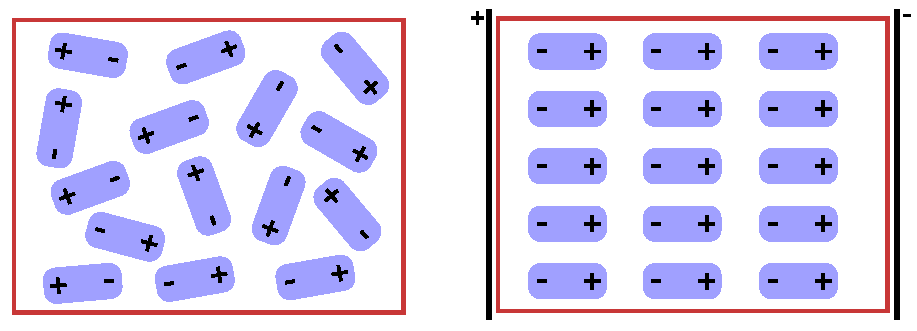
\psfig{file=fig/fig-dielectrico-01.pdf,height=4cm,angle=0}}
\caption{Un material diel'ectrico se polariza en presencia de un campo externo.}
\label{diel01}
\end{figure}

El campo el'ectrico total (``EL''\, campo el'ectrico) es influenciado por
la polarizaci'on del medio. Modelaremos este campo el'ectrico
(macrosc'opico) $\vec{E}$ como la suma del campo
producido por las cargas externas y el campo producido por la distribuci'on
de \textit{cargas de polarizaci'on} (descrita por el vector de polarizaci'on $\vec{P}$) del medio.

\subsection{Vector y cargas de Polarizaci'on}

Se define el \textit{vector de polarizaci'on} como la \textit{densidad de
momento dipolar} (momento dipolar por unidad de volumen),
\begin{equation}\label{defP}
\vec{P}(x):= ``\lim_{\Delta V\to 0}" \frac{\Delta\vec{p}}{\Delta V},
\end{equation}
donde $\Delta\vec{p}$ es el \textit{momento dipolar total de las cargas del material contenidas en el volumen} $\Delta V$. La regi'on con volumen $\Delta V$ se considera centrada en el punto $\vec{x}$, suficientemente peque\~na desde el punto de vista macrosc'opico, pero grande comparada con la escala  determinada por la estructura at'omica/molecular del material. Equivalentemente, el vector de polarizaci'on es definido tal que el momento dipolar $d\vec{p}$ en un elemento de volumen (macrosc'opico) $dV$ es dado por $d\vec{p}=\vec{P}(\vec{x})dV$.

Como consecuencia de la definici'on anterior, el momento dipolar
total de las cargas contenidas en un volumen finito $V$ es dado por
\begin{equation}\label{pintPdV}
 \vec{p}_V=\int_V \vec{P}(x)\,dV.
\end{equation}
Por otro lado, sabemos que el potencial generado por un dipolo ideal de momento dipolar $\vec{p}$ ubicado en un punto con coordenadas $\vec{x}'$ es de la forma \eqref{phip}. Luego, el potencial generado por una peque\~na regi'on de un medio polarizado con elemento de volumen $dV'$ y polarizaci'on $\vec{P}$ es dada por
\begin{equation}
d\phi(x)=\frac{1}{4\pi\varepsilon_0}\frac{(x_j-x_j')P_j(x')\,dV'}{|\vec{x}-\vec{
x}'|^3}.
\end{equation}
De esta forma, si el sistema contiene adem'as cargas libres en $dV'$ entonces
\begin{equation}
d\phi(x)=\frac{1}{4\pi\varepsilon_0}\frac{\rho_{\rm
ext}(x')}{|\vec{x}-\vec{x}'|}dV'+\frac {1}{
4\pi\varepsilon_0}\frac{P_i(x')(x_i-x_i')}{|\vec{x}-\vec{x}'|^3}dV'.
\end{equation}
Por lo tanto, el potencial (macrosc'opico, total), de acuerdo a nuestro modelo, es dado por
\begin{equation}
\boxed{\phi(x)=\frac{1}{4\pi\varepsilon_0}\int\left[\frac{\rho_{\rm
ext}(x')}{|\vec{x}-\vec{x}'|}+\frac{P_i(x')(x_i-x_i')}{|\vec{x}-\vec{x}'|^3}\right]dV'.}
\end{equation}
Usando la identidad (\ref{id01}) podemos escribir
\begin{align}
\frac{P_i(x')(x_i-x_i')}{|\vec{x}-\vec{x}'|^3}  &
=P_i(x')\partial_i'\left(  \frac{1}{|\vec{x}-\vec{x}'|}\right)\\
&=\partial_i'\left(\frac{P_i(x')}{|\vec{x}-\vec{x}'|}\right)-\frac{
(\partial_i'P'_i)(x')} {|\vec{x}-\vec{ x}'|}.
\end{align}
De esta forma, considerando que la integral sobre los t'erminos que dependen de la polarizaci'on est'an confinados al volumen $V$ del material (lo que no necesariamente es as'i para el t'ermino conteniendo las cargas libres), podemos escribir
\begin{align}
\phi(x)& =\frac{1}{4\pi\varepsilon_0}\int\frac{\rho_{\rm ext}(x')}{|x_i-x_i'|}dV'-\frac{1}{4\pi\varepsilon_0}\int_V\frac{1}
{|\vec{x}-\vec{x}'|}\partial_i'P_idV'+\frac{1}{4\pi\varepsilon_0}\int_{
\partial V}\frac{P_i(x')}{|\vec{x}-\vec{x}'|}\,dS'_i \\
& =\frac{1}{4\pi\varepsilon_0}\int\frac{\rho_{\rm ext}(x')}{|x_i-x_i'|}dV'+\frac{1}{4\pi\varepsilon_0}\int_V\frac{\rho_P(x')}{|x_i-x_i'|}dV'+\frac{1}{4\pi\varepsilon_0}\int_{
\partial V}\frac{\sigma_P(x')}{|\vec{x}-\vec{x}'|}\,dS' .
\end{align}
La expresi'on anterior muestra que el campo (macrosc'opico) total es
\textit{equivalente} al campo producido por una densidad volum'etrica de carga total,
\begin{equation}
\rho_{\rm T}:=\rho_{\rm ext}+\rho_P, \label{rhotot}
\end{equation}
donde
\begin{equation}
\boxed{\rho_P:=-\vec{\nabla}\cdot\vec{P},}
\end{equation}
es la \textit{densidad (volum'etrica) de carga de polarizaci'on}, (definida en cada punto del material), m'as una
\textit{densidad de carga de polarizaci'on de superficie},
\begin{equation}
\boxed{\sigma_P:=\vec{P}\cdot\hat{n},}
\end{equation}
distribuida en la superficie $S=\partial V$ del diel'ectrico.

Note que la carga total de polarizaci'on, tal como se espera, es nula:
\begin{equation}
 Q_P=\int_V\rho_P\,dV+\oint_{\partial V} \sigma_P\,dS\equiv 0,
\end{equation}
en virtud del teorema de Gauss.

\subsection{Desplazamiento el'ectrico}
Usando (\ref{rhotot}) en la ley de Gauss, podemos escribir
\begin{align*}
\vec\nabla\cdot\vec{E} &=\frac{1}{\varepsilon_0}\rho_T \\
&=\frac{1}{\varepsilon_0}\left( \rho_{\rm ext}-\vec\nabla\cdot\vec{P}\right).
\end{align*}
Luego,
\begin{equation}
 \vec\nabla\cdot\left(\vec{E}+\frac{1}{\varepsilon_0}\vec{P}\right)=\frac{\rho_{
\rm ext}(x)}{\varepsilon_0}.
\end{equation}
Definimos el \textit{vector de desplazamiento el'ectrico} (tambi'en llamado
\textit{excitaci'on el'ectrica} o \textit{inducci'on el'ectrica}) como
\begin{equation}\marginnote{Vector Desplazamiento}
 \boxed{\vec{D}(\vec{x}):=\varepsilon_0\vec{E}(\vec{x})+\vec{P}(\vec{x}),} \label{defD}
\end{equation}
de modo que
\begin{equation}
\boxed{\vec{\nabla}\cdot\vec{D}=\rho_{\rm ext}.} \label{divD}
\end{equation}
Las unidades del vector desplazamiento son de carga por unidad de 'area: 
$[\vec{D}]=[\vec{P}]=[\sigma]\stackrel{\text{
S.I.}}{=}{C}/{m^2}$.

La utilidad de usar $\vec{D}$ en lugar de $\vec{E}$ en esta ``ley de Gauss"
\,\eqref{divD} es que esta relaci'on \textit{s'olo involucra expl'icitamente a las cargas externas} (que son usualmente conocidas y/o controlables). Por ejemplo, como consecuencia de (\ref{divD}) tenemos que
\begin{equation}
 \boxed{\oint_S \vec{D}\cdot d\vec{S}=q_{\rm ext}.} \label{GaussD}
\end{equation}

\subsubsection{Ejemplo: Esfera diel'ectrica is'otropa y carga central}
\begin{figure}[!h]
\centerline{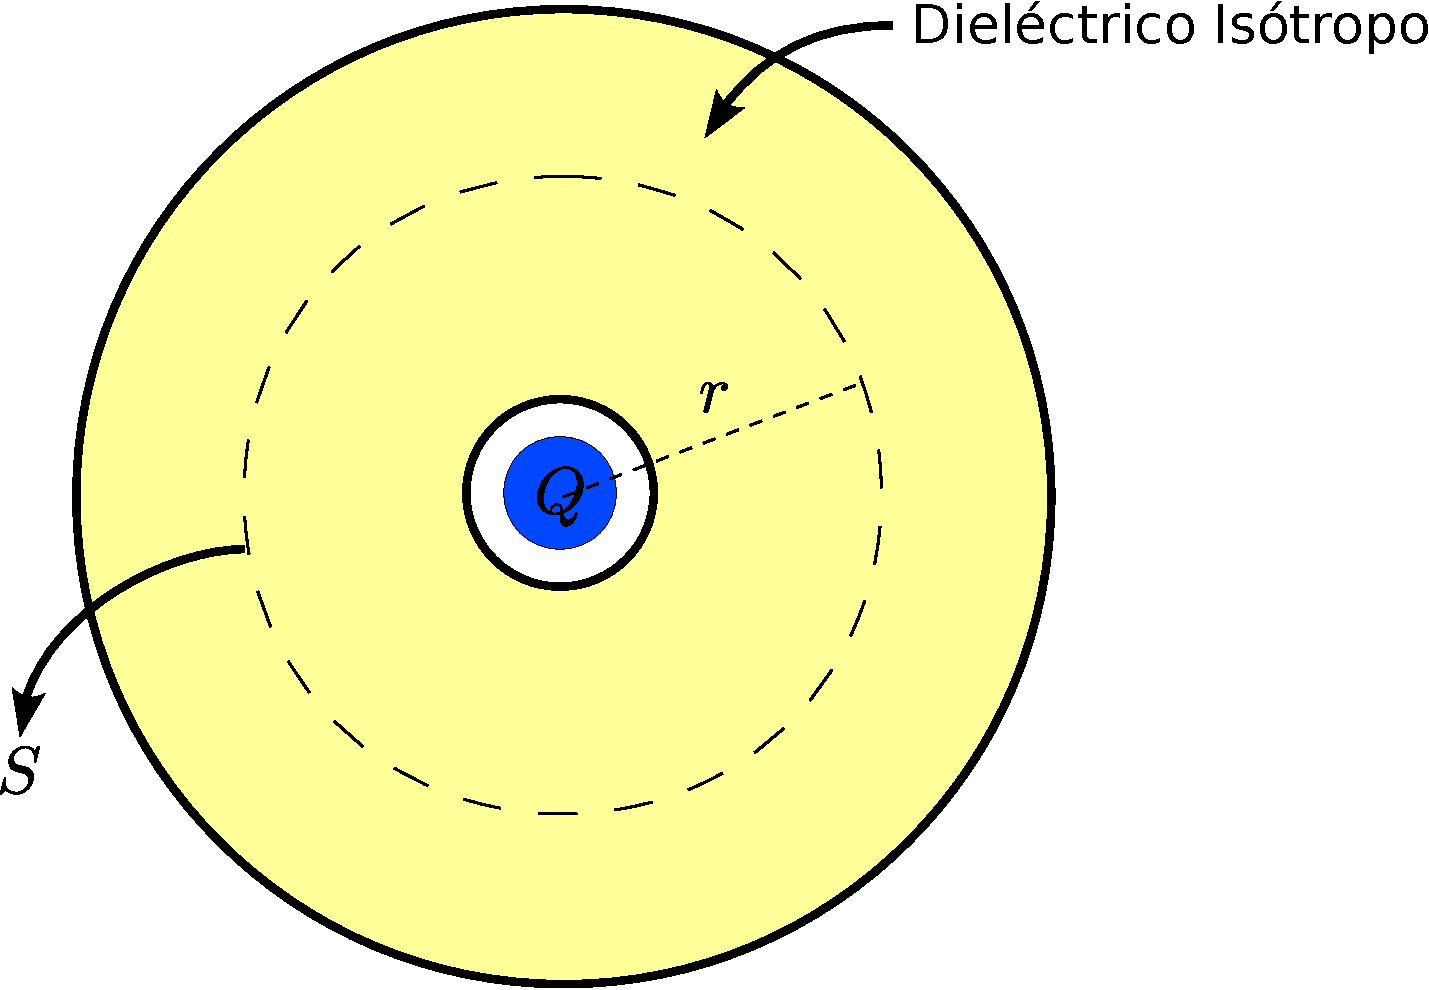
\psfig{file=fig/fig-dielectrico-y-carga-01.pdf,height=4cm,angle=0}}
\caption{Un material diel'ectrico is'otropo con una carga central.}
\label{diel02}
\end{figure}
Consideremos una carga (externa) $Q$ situada en el centro de una
esfera diel'ectrica \textit{is'otropa}, ver figura \ref{diel02}, podemos encontrar el vector de desplazamiento aplicando (\ref{GaussD}). Debido a la simetr'ia del sistema (ya que asumimos que el diel'ectrico es \textit{is'otropo}, ver secciones \ref{sec:aniso} y \ref{sec:iso}), tendremos que $\vec{D}(\vec{x})=D(r)\hat{r}$. Eligiendo una superficie Gaussiana esf'erica de radio $r$ centrada en la carga $Q$, encontramos entonces que
\begin{equation}
 D(r)\oint_S dS=D(r)4\pi r^2=Q,
\end{equation}
y por lo tanto
\begin{equation}
 \vec{D}(\vec{x})=\frac{Q}{4\pi}\frac{1}{r^2}\,\hat{r}.
\end{equation}


\subsection{Relaci'on Constitutiva, susceptibilidad, permeabilidad}

Cada medio se caracteriza por la polarizaci'on $\vec{P}(\vec{x})$ que presenta,
dados los campos/cargas externas. Esta polarizaci'on $\vec{P}(\vec{x})$ depende
entonces de los campos/cargas externas y de la constituci'on at'omica/molecular
del material (y en principio de otras propiedades, como la temperatura,
presi'on, etc). 
%Equivalentemente, esta informaci'on acerca de las propiedades
%del material puede expresarse en la relaci'on entre el campo el'ectrico
%$\vec{E}(\vec{x})$ y el vector desplazamiento el'ectrico $\vec{D}(\vec{x})$.

En un elemento de volumen dado del medio 'este modificar'a su distribuci'on microsc'opica de cargas como respuesta al campo el'ectrico ``total"\,que act'ua sobre este elemento, hasta finalmente adoptar un cierta polarizaci'on. Podemos, por tanto, considerar que $\vec{P}=\vec{P}(\vec{E})$ o, equivalentemente
$\vec{D}=\vec{D}(\vec{E})$. Esta 'ultima relaci'on es llamada
\textit{relaci'on constitutiva} del medio. El problema es que el campo
$\vec{E}(\vec{x})$ en un punto dado (con vector de polarizaci'on $\vec{P}(\vec{x})$ y
por tanto desplazamiento $\vec{D}(\vec{x})$) depende tambi'en de c'omo se
polariza el medio \textit{en otras regiones}, e.d., $\vec{E}(\vec{x})$ depende
en general de\footnote{Matem'aticamente, esto significa que, en
general, $\vec{E}$ es un \textit{funcional}, una ``funci'on de funciones''\, o
una ``funci'on no-local''\, de $\vec{P}$.} $\vec{P}(\vec{x}')$.
En otras palabras, en general la polarizaci'on que se presentar'a en un medio es fruto de la  \textit{respuesta colectiva} del material a los campos externos.

 Vemos entonces que calcular $\vec{P}(\vec{x})$ desde ``primeros principios'' es en gerenal dif'icil y requiere conocer los detalles de la estructura del material en estudio.

Existe una gran variedad de medios materiales con propiedades el'ectricas
diferentes e interesantes. Existen por ejemplo medios que tienen \textit{polarizaci'on
no nula a'un en ausencia de campos/cargas externas}. Estos medios son conocidos
como \textit{electretos} (an'alogos el'ectricos de los im'anes permanentes), y 
\textit{ferroel'ectricos} (que presentan polarizaci'on no nula bajo una cierta
temperatura cr'itica, de Curie, an'alogamente a los ferromagnetos). Un ejemplo
de material ferroel'ectrico es el $BaTiO_3$ (titanato de bario), que exhibe un
momento dipolar el'ectrico no nulo a temperaturas bajo $120^{\rm o}\,C$. Un ejemplo de electreto es el cuarzo ($SiO_2$, di'oxido de Silicio), que presenta \textit{propiedades piezoel'ectricas}.

Es 'util adem'as distinguir entre distintos tipos de polarizaci'on, dependiendo del mecanismo que gobierne dicha propiedad: \textit{polarizaci'on electr'onica}, p.ej. cuando un 'atomo se ``deforma"\,en presencia de un campo externo; \textit{polarizaci'on i'onica}, causada por arreglo de iones (p.ej. $NaCl$); \textit{polarizaci'on polar} que se manifiesta en los gases (cuando la
temperatura aumenta, disminuye la polarizaci'on porque las mol'eculas se
``desordenan").

M'as a'un, en algunos materiales (``no-lineales''\,) la respuesta
(polarizaci'on) del material puede depender no-linealmente del campo el'ectrico.

Sin embargo, existe una gran variedad de materiales que, desde el punto de
vista macrosc'opico, pueden ser modelados adecuadamente (es decir, con \textit{precisi'on suficiente} en la mayor'ia de las situaciones) por una relaci'on lineal entre $\vec{D}$ y $\vec{E}$. Un \textit{material lineal}, pero en general \textit{no-local}, puede describirse a
trav'es de una relaci'on de la forma
\begin{equation}
D_i[\vec{E}](\vec{x},t)=\int
f_{ij}(\vec{x},\vec{x}',t,t')\,{E}_j(\vec{x}',t')\,dV' dt',
\end{equation}
donde $f_{ij}(\vec{x},\vec{x}',t,t')$ es un cierto tensor que describe las
propiedades del medio. Como la polarizaci'on y por tanto el vector
desplazamiento en un punto $\vec{x}$ del medio est'an influenciadas en forma
m'as determinante por lo que le ocurre al material en la inmediata vecindad de
$\vec{x}$ es de esperar que la funci'on $f_{ij}(\vec{x},\vec{x}',t,t')$ sea
concentrada en torno a $\vec{x}$, es decir, que decaiga r'apidamente para
$|\vec{x}'-\vec{x}|\gg d$ donde $d$ es la escala caracter'istica de la
estructura microsc'opica del medio.

Por otro lado, existen muchos casos en que es \textit{suficiente} considerar una
\textit{relaci'on constitutiva local} en la que el vector desplazamiento en un
punto dado puede modelarse como dependiendo exclusivamente del valor del campo
el'ectrico \textit{en el mismo punto} (macrosc'opico), es decir
$\vec{D}(\vec{x})=\vec{D}(\vec{E}(\vec{x}))$ o, equivalentemente
$\vec{P}(\vec{x})=\vec{P}(\vec{E}(\vec{x}))$.

En un material descrito por una relaci'on constitutiva local podemos considerar
la dependencia de $\vec{P}$ con $\vec{E}$ a trav'es de una expansi'on en serie
de la forma:
\begin{equation}\label{expP}
P_i(x)=P_i(E_j(x))=(P_i)_{\vec{E}=\vec{0}}
+E_j(\partial_jP_i)_{\vec{E}=\vec{0}}+\frac{1}{2}
E_jE_k(\partial_j\partial_k P_i)_{\vec{E}=\vec{0}}+\cdots,
\end{equation}
que esperamos sea 'util para campos el'ectricos suficientemente d'ebiles (en el
presente contexto s'olo podemos saber \textit{a posteriori} qu'e tan d'ebil
requiere ser el campo). Note que en el lado derecho de (\ref{expP}) las derivadas $\partial_i$ denotan derivadas respecto a la componente $i$-'esima del campo el'ectrico, es decir $\partial_iP_j={\partial P_j}/{\partial E_i}$, etc.. Las cantidades $(P_i)_{\vec{E}=\vec{0}}$,
$(\partial_jP_i)_{\vec{E}=\vec{0}}$,
$(\partial_j\partial_k P_i)_{\vec{E}=\vec{0}}$, etc. son
tensores (cartesianos) que asumen diferentes valores para cada material y pueden ser
considerados como par'ametros (a determinar). Con esto, podemos escribir
\begin{equation}
\boxed{P_i(x)={\cal A}_i+{\cal A}_{ij}E_j+{\cal A}_{ijk}
E_jE_k+\cdots.}
\end{equation}
En general, si el material es \textit{inhomog'eneo} (por ejempo, si est'a formado por
capas de distintos materiales), los tensores ${\cal A}_i$, ${\cal A}_{ij}$, ${\cal A}_{ijk}$, etc. depender'an de la posici'on. Para materiales no-ferroel'ectricos (la gran mayor'ia) tenemos que ${\cal A}_i=0$.



\subsection{Medios lineales anis'otropos}\label{sec:aniso}

Adicionalmente, si la polarizaci'on de un material es descrita apropiadamente
por una relaci'on lineal, como ocurre en el caso de campos el'ectricos
suficientemente d'ebiles, tendremos
\begin{equation}
\boxed{P_i(x)=\varepsilon_0\chi_{ij}(x)E_j(x),} \label{rcml}
\end{equation}
entonces decimos que el medio es \textit{lineal}. El tensor $\chi_{ij}$ es
llamado \textit{tensor de susceptibilidad el'ectrica} del medio.  El factor $\varepsilon_0$ es incluido de modo que $\chi_{ij}$ es un tensor adimensional. En este caso,
usando (\ref{defD}) y (\ref{rcml}), tenemos que
\begin{equation}\label{rclai}
\boxed{D_i(x)=\varepsilon_{ij}(x)E_j(x)=\varepsilon_0\,\kappa_{ij}(x)E_j(x),}
\end{equation}
donde hemos definido el \textit{tensor de permitividad} del medio
$\varepsilon_{ij}$, por
\begin{equation}
\varepsilon_{ij}:=\varepsilon_0(\delta_{ij}+\chi_{ij})
\end{equation}
y, alternativamente,  el \textit{tensor diel'ectrico},
\begin{equation}
\kappa_{ij}:=\frac{1}{\varepsilon_0}\varepsilon_{ij}=\delta_{ij}+\chi_{ij},
\end{equation}
que tiene la ventaja de ser una cantidad adimensional.

Es posible probar por
argumentos energ'eticos que si el medio no es disipativo (no existen mecanismos
de transferencia de energ'ia del campo el'ectrico a otras formas de energ'ia)
entonces necesariamente $\chi_{ij}$ (y por tanto $\varepsilon_{ij}$ y
$\kappa_{ij}$) es un tensor \textit{sim'etrico} y que posee, por lo
tanto, 6 componentes independientes. La descripci'on de las
propiedades de un medio lineal a trav'es de un tensor de susceptibilidad
el'ectrica incluye el caso en que el medio sea \textit{anis'otropo}, es decir,
que sus propiedades no sean invariantes bajo rotaciones o, en otras palabras,
que posea ciertas \textit{direcciones preferentes}. En un medio anis'otropo, la
polarizaci'on no ser'a en general paralela al campo el'ectrico (excepto para las
direcciones preferentes dadas por las direcciones principales. Ver secci'on
\ref{secDP}.), esto como
resultado de la estructura microsc'opica del material (t'ipicamente, cristales),
que tienen como consecuencia que el material se polarize en algunas direcciones
m'as f'acilmente que en otras.


Note que en el caso m'as general en que se consideran campos el'ectricos dependientes del tiempo (esto es necesario, por ejemplo, en el caso de propagaci'on de ondas electromagn'eticas), a'un cuando un medio pueda considerarse lineal y local respecto a su dependencia con la posici'on, la relaci'on constitutiva es de la forma
\begin{equation}
D_i(x,t)=\int f_{ij}(t,t')E_j(x,t')\,dt'.
\end{equation}
En estos casos es conveniente considerar las \textit{transformadas de Fourier temporal} de los campos, es decir $\tilde{D}_i(x,\omega)$, $\tilde{E}_i(x,\omega)$, etc., ya que permiten escribir la relaci'on constitutiva como
\begin{equation}\label{RELtilde}
\tilde{D}_i(x,\omega)=\tilde{\varepsilon}_{ij}(x,\omega)\tilde{E}_j(x,\omega). 
\end{equation}
Comparando \eqref{RELtilde} con \eqref{rclai} vemos que en el caso m'as general, el tensor $\tilde{\varepsilon}_{ij}(x,\omega)$ juega un rol an'alogo a $\varepsilon_{ij}$ en \eqref{rclai} y tambi'en es llamado, por esta raz'on, el tensor diel'ectrico del medio. Note, sin embargo, que este tensor \textit{asume valores complejos y depende en general de la frecuencia} $\omega$.


\subsection{Medios lineales is'otropos}\label{sec:iso}
Si el material es is'otropo, es decir, si 'este no posee ninguna direcci'on
preferente, la polarizaci'on debe necesariamente ser paralela al campo
el'ectrico, independientemente de la direcci'on de este 'ultimo. Esta condici'on requiere que el tensor de susceptibilidad sea proporcional al tensor identidad,
\begin{equation}
\chi_{ij}=\chi\,\delta_{ij},
\end{equation}
de modo que
\begin{equation}
\vec{P}=\varepsilon_0\chi\vec{E}.
\end{equation}
Muchos materiales presentan propiedades de polarizaci'on independientes de
la direcci'on del campo el'ectrico, es decir, son is'otropos. Por ejemplo, los
gases, l'iquidos (excepto los, as'i llamados, \textit{cristales liquidos}), s'olidos amorfos (pl'asticos, vidrio).
Los medios no-lineales, pero is'otropos, pueden ser descritos usando
$\vec{P}=\varepsilon_0\chi(|\vec{E}|)\vec{E}$.

En este curso, a menos que se explicite lo contrario, consideramos siempre
materiales lineales, is'otropos y homog'eneos. En este caso, es suficiente
introducir la (``constante de''\,) permitividad y/o la constante diel'ectrica
por
\begin{equation}
\varepsilon:=\varepsilon_0(1+\chi), \qquad
\kappa:=\frac{\varepsilon}{\varepsilon_0}=1+\chi.
\end{equation}
Note que en un medio polarizable es de esperar que $\chi>0$, de modo que
$\varepsilon>\varepsilon_0$ o, equivalentemente, $\kappa>1$. El vac'io puede ser
considerado como un ``medio is'otropo''\, con $\chi=0$ y $\kappa=1$, es decir, no polarizable.
Recuerde tambi'en que el 'indice de refracci'on de la mayor'ia de los medios
(``no-magn'eticos''\,) es dado por $n\approx\sqrt{\kappa}$.
\begin{table}[!h]
\begin{center}
\begin{tabular}{c|c}
Material &   $\kappa$ \\ \hline\hline
Vac'io & 1 \\
Aire (seco, $0^{\rm o}$C, 1 bar)  & 1,00059 \\
Agua ($110^{\rm o}$C, 1 bar)  & 1,0126 \\
Agua ($20^{\rm o}$C) &  80,0 \\
Hielo ($-30^{\rm o}$C) &  99 \\
$SrTiO_3$ (cristal, $10$K)  & 12.000 \\
\end{tabular}
\caption{Algunos materiales is'otropos y sus constantes diel'ectricas.}
\end{center}
\end{table}

\subsection{Ecuaci'on de Poisson y su generalizaci'on}

Usando (\ref{divD}) y (\ref{E=nablaphi}) encontramos la generalizaci'on de la
ecuaci'on de Poisson para el potencial en un diel'ectrico lineal y local:
\begin{equation}
 \boxed{\partial_i\left(\kappa_{ij}\,\partial_j \phi\right)
=-\frac{1}{\varepsilon_0}\rho_{\rm ext}.}
\end{equation}
Para un material homog'eneo e is'otropo, esta ecuaci'on se reduce a
\begin{equation}\label{Poissond}
 \boxed{\nabla^2\phi=-\frac{1}{\varepsilon}\rho_{\rm ext},}
\end{equation}
que tiene la misma forma (matem'aticamente, es la \textit{misma} ecuaci'on) que
en caso del campo en el vac'io ($\varepsilon=\varepsilon_0$). Finalmente, en
regiones fuera de cargas externas (!`\,pero \textit{no} de cargas de
polarizaci'on!), el potencial satisface la ecuaci'on de Laplace. Como
consecuencia, es posible usar las t'ecnicas conocidas para solucionar esta ecuaci'on, por ejemplo, expansi'on en funciones especiales, o funciones de Green, en el caso de los diel'ectricos.
Como veremos a continuaci'on, una diferencia importante respecto al caso en el
vac'io ser'a la implementaci'on de las condiciones de borde o frontera.


\subsection{Direcciones principales de un medio anis'otropo}\label{secDP}

Como vimos, en un medio anis'otropo, el campo el'ectrico no tiene en general
la misma direcci'on que el vector desplazamiento.
Existen, sin embargo, direcciones ``especiales''\, a lo largo de las cuales el
campo el'ectrico s'i tiene la misma direcci'on que la polarizaci'on. Esto significa
que, si $\hat{n}$ es una de estas direcciones, conocidas como \textit{direcciones
principales} del material, entonces $\vec{E}=E\hat{n}$ y $\vec{D}=D\hat{n}$.
Insertando estas condiciones en (\ref{rclai}) obtenemos que
\begin{equation}
\kappa_{ij}\,\hat{n}_j= \lambda\,\hat{n}_i, \qquad D=\varepsilon_0\lambda E.
\end{equation}
Vemos de aqu'i que las direcciones principales corresponden a los vectores
propios de la matriz  $\kappa_{ij}$, mientras que el valor propio $\lambda$ es
el valor de la constante diel'ectrica del material a lo largo de aquella
direcci'on principal. Como la matriz $\kappa_{ij}$ es real y sim'etrica, es
posible encontrar tres vectores propios ortonormales, es decir, una base
ortonormal formada por las direcciones principales del material. Existen
distintos casos particulares e interesantes de materiales anis'otropos
correspondiendo a si los valores propios son todos diferentes o iguales. Si
todos los valores propios son iguales, el material es is'otropo, puesto que en
ese caso $\kappa_{ij}=\lambda\,\delta_{ij}$. Si dos valores propios son iguales
y uno diferente, se dice que el material es \textit{uniaxial} (puesto que
tienen una direcci'on distintiva, aquella descrita por el vector propio del
valor propio distinto a los otros dos. Esta direcci'on es llamada \textit{eje
'optico}). Un ejemplo de material uniaxial natural es la Calcita ($CaCO_3$). En
materiales uniaxiales la propagaci'on de la luz presenta el fen'omeno llamado
\textit{birefringencia}, en los que la luz en su interior se propaga, en
general, por dos trayectorias diferentes (rayo ``ordinario''\, y
``extraordinario'') correspondientes a dos 'indices de refracci'on diferentes.
Adem'as, es posible inducir anisotrop'ia (y por tanto, en general,
birefringencia), comprimiendo un material en una direcci'on dada, o
con un campo el'ectrico intenso externo (\textit{efecto Kerr}). Finalmente, si
los tres valores propios del tensor diel'ectrico son diferentes, entonces el
material (t'ipicamente un cristal) es llamado \textit{biaxial}.

\begin{table}[!h]
\begin{center}
\begin{tabular}{l c |c| c}
Mineral 		& 	F'ormula qu'imica 	&	$n_{\rm o}=\sqrt{\kappa_\perp}$	& 	$n_{\rm e}=\sqrt{\kappa_\parallel}$
%& 	 $\Delta n=n_e-n_o$
\\
\hline\hline
Berilo 			& Be$_3$Al$_2$(Si6O18)	&	1.602	& 	1.557	
%&	-0.045	
\\
Calcita 		&	CaCO$_3$  	&	1.658	& 	1.486	
%& 	-0.172	
\\
%Calomelano 		&	Hg$_2$Cl$_2$	& 	1.973	& 	2.656	
%& 	+0.683	
%\\
%cinnabar 		&	HgS    		&	2.905	& 	3.256	
%& 	+0.351	
%\\
Hematita 		&	Fe$_2$O$_3$	&	2.940	& 	3.220	
%& 	+0.287	
\\
Hielo 			&	H$_2$O 		&	1.309	&	1.313	
%& 	+0.014	
\\
Niobiato de litio 	&	LiNbO$_3$	&	2.272	& 	2.187	
%& 	-0.085	
\\
Fluoruro de magnesio 	&	MgF$_2$		&	1.380	& 	1.385	
%& 	+0.006	
\\
Quarzo 			&	SiO$_2$		&	1.544	& 	1.553	
%& 	+0.009	
\\
Rub'i 			& Al$_2$O$_3$:Cr	&	1.770 	&	1.762	
%& 	-0.008	
\\
%Rutilo 			&	TiO$_2$ 		&	2.616	& 	2.903	
%& 	+0.287	
%\\
%Peridot 		&	  		&	1.690	& 	1.654	
%& 	-0.036	
%\\
Zafiro	 		&	Al$_2$O$_3$	&	1.768	& 	1.760	
%& 	-0.008	
\\
Nitrato de sodio	&	NaNO$_3$	&	1.587	& 	1.336	
%& 	-0.251	
%\\
%Turmalina 		&	  		&	1.669	& 	1.638	
%& 	-0.031	
\\
Circ'on, high 		&	ZrSiO$_4$	&	1.920 -1.960	&  1.967-2.015	
%& +0.047; +0.055	
\end{tabular}
\caption{Algunos cristales uniaxiales y sus 'indices de refracci'on. Datos tabulados para $\lambda\sim 590\,{\rm [nm]}$ \cite{hyper}.}
\end{center}
\end{table}

\begin{table}[!h]
\begin{center}
\begin{tabular}{l c |c|c|c}
Mineral			& F'ormula qu'imica		& $\sqrt{\kappa_x}$	&	$\sqrt{\kappa_y}$	&  $\sqrt{\kappa_z}$	\\
\hline\hline
B'orax 	 		&Na$_2$B$_4$O$_7$·10H$_2$O& 	1.447	& 	1.469	& 	1.472	\\
Sulfato de magnesio		&  MgSO$_4$·7(H$_2$O)	& 	1.433	& 	1.455	& 	1.461	\\
%Biotita		&			&  	1.595	& 	1.640	& 	1.640	\\
%Moscovita		&			&  	1.563	& 	1.596	& 	1.601	\\
Olivina			& 	(Mg,Fe)2SiO	& 	1.640	& 	1.660	& 	1.680	\\
Perovskita		& 	CaTiO$_3$	& 	2.300	& 	2.340	& 	2.380	%\\
%Topacio			&			&  	1.618	& 	1.620	& 	1.627	\\
%Ulexita			&			&  	1.490	& 	1.510	& 	1.520	
\end{tabular}
\caption{Algunos cristales biaxiales. Datos tabulados para $\lambda\sim 590\,{\rm [nm]}$ \cite{hyper}.}
\end{center}
\end{table}
\subsection{Condiciones de frontera para $\vec{D}$}

El vector desplazamiento el'ectrico satisface la ecuaci'on (\ref{divD}), que es
de la misma forma que la ley de Gauss (\ref{leygauss-dif}), con la diferencia
que en (\ref{divD}) el factor $\varepsilon_0$ est'a ausente y que la densidad de carga en el lado derecho es s'olo la densidad de cargas externas (\underline{no} las de polarizaci'on). Como consecuencia, podemos aplicar el mismo procedimiento discutido en la secci'on \ref{secCBE} para derivar las condiciones que el vector desplazamiento debe satisfacer en la frontera de dos materiales. Consideramos una superficie que divide dos diel'ectricos de propiedades diferentes, en la que, eventualmente, existe una densidad de carga externa $\sigma_{\rm ext}$. Si $\hat{n}$ es el vector unitario normal a la superficie en un punto dado, que apunta desde el material 1 hasta el 2, entonces
\begin{figure}[!h]
\centerline{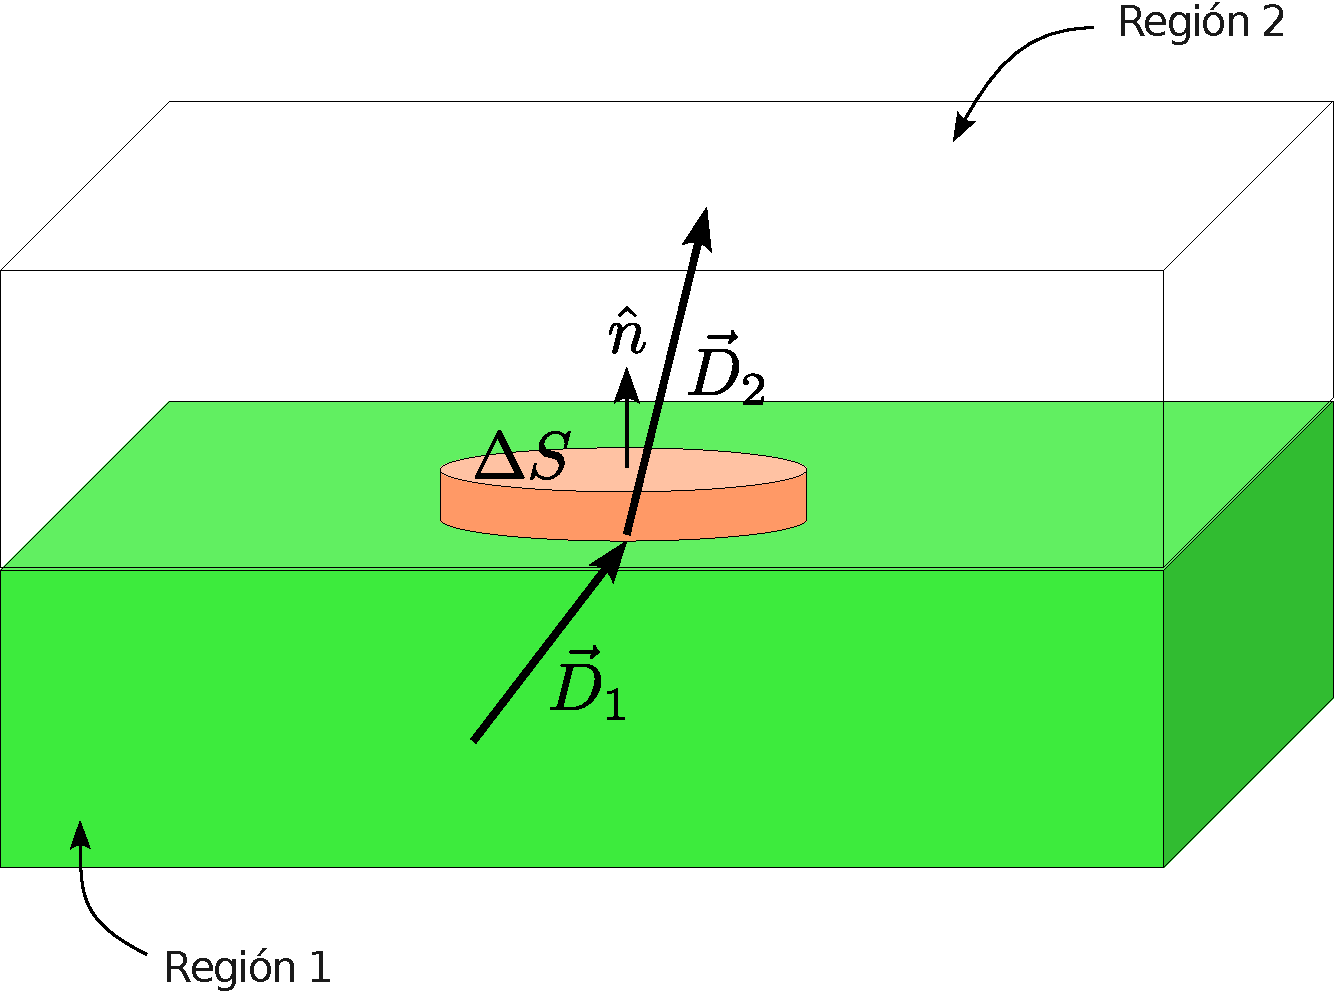
\psfig{file=fig/fig-dielectrico-condicion-borde-01.pdf,height=5cm,
angle=0}}
\caption{La componente normal del vector desplazamiento puede ser discontinua
si existen cargas externas en el la interfase entre dos diel'ectrico.}
\label{CF1}
\end{figure}
\begin{equation}\label{saltoDn}
\boxed{\vec{D_2}\cdot\hat{n}-\vec{D_1}\cdot\hat{n}=\sigma_{\rm
ext}.}
\end{equation}

Por otro lado, el campo el'ectrico $\vec{E}$ sigue satisfaciendo (\ref{rotE0}),
de modo que, como consecuencia, su componente tangencial es continua a trav'es
de la superficie, tal como lo expresa la condici'on (\ref{Etconst}). Recuerde
finalmente que el potencial el'ectrico siempre es una funci'on continua, de
modo que el campo el'ectrico, aunque eventualmente discontinuo, es finito en
todo punto.
\begin{figure}[!h]
\centerline{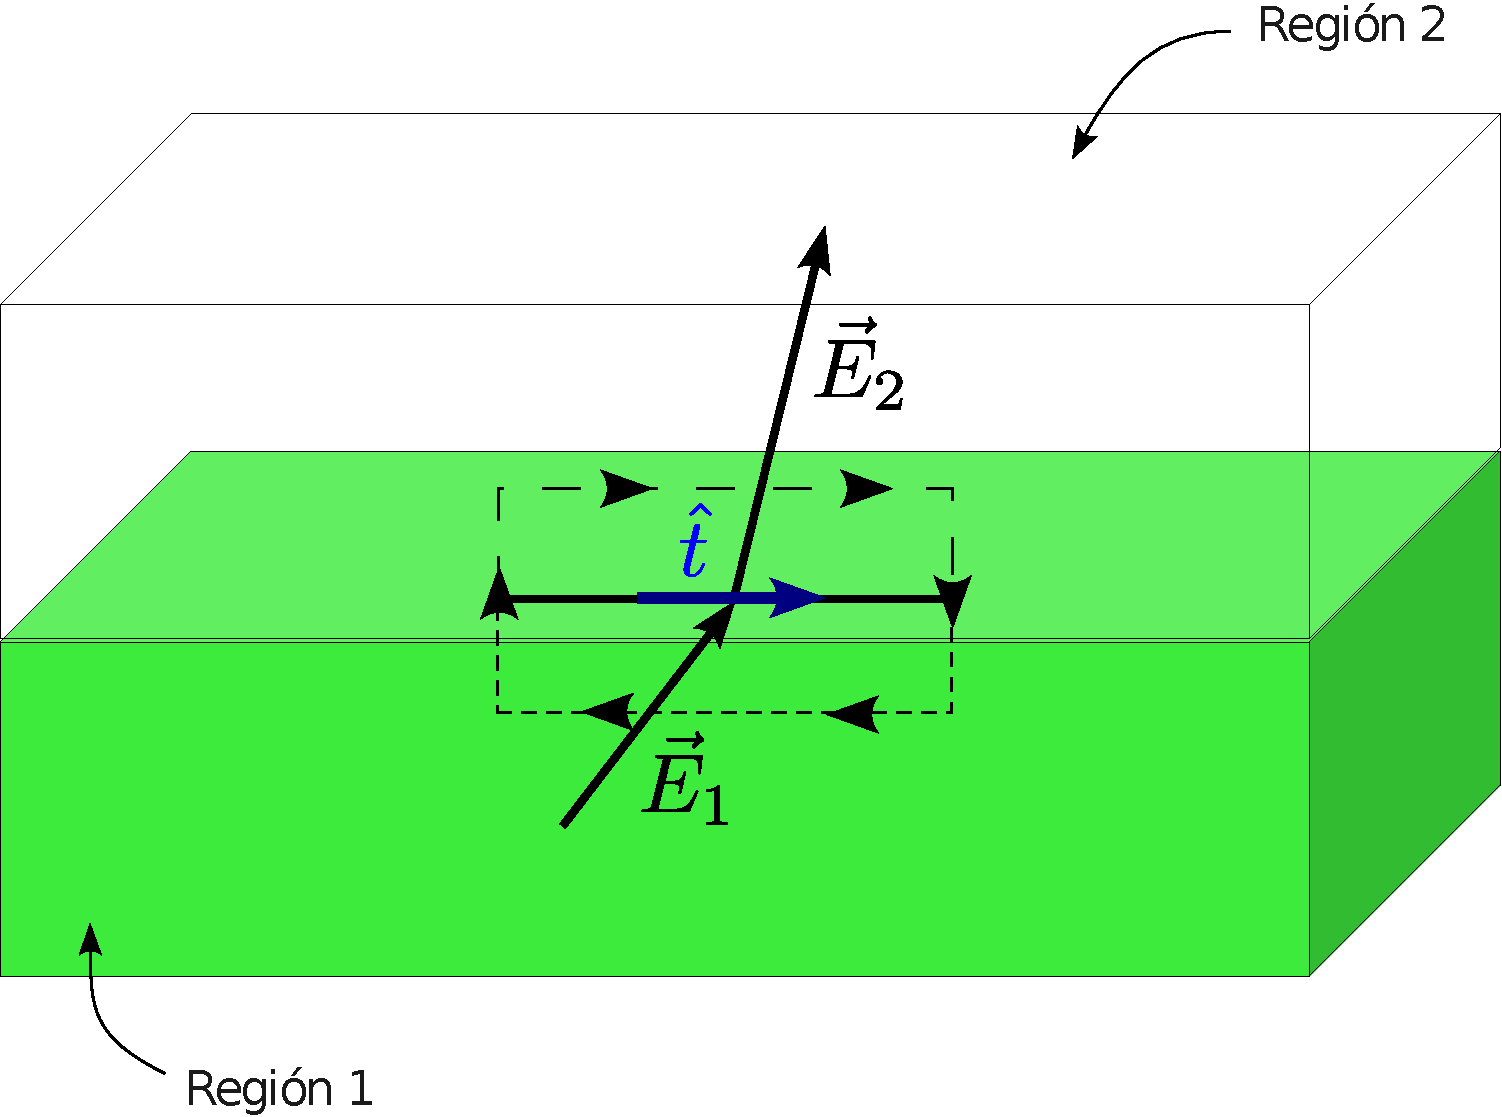
\psfig{file=fig/fig-dielectrico-condicion-borde-02.pdf,height=5cm,
angle=0}}
\caption{La componente tangencial del campo el'ectrico es siempre continua
en una interfase.}
\label{CF2}
\end{figure}

\subsection{Caso de un medio lineal e is'otropo}

Consideramos aqu'i el caso particular de medios lineales e is'otropos caracterizados por las constantes diel'ectricas $\kappa_1$ y $\kappa_2$ respectivamente. Consideramos adem'as el 'angulo entre los vectores campo el'ectrico a cada lado de la superficie y el vector normal. Ver figura \ref{CF3}. 
\begin{figure}[!h]
\centerline{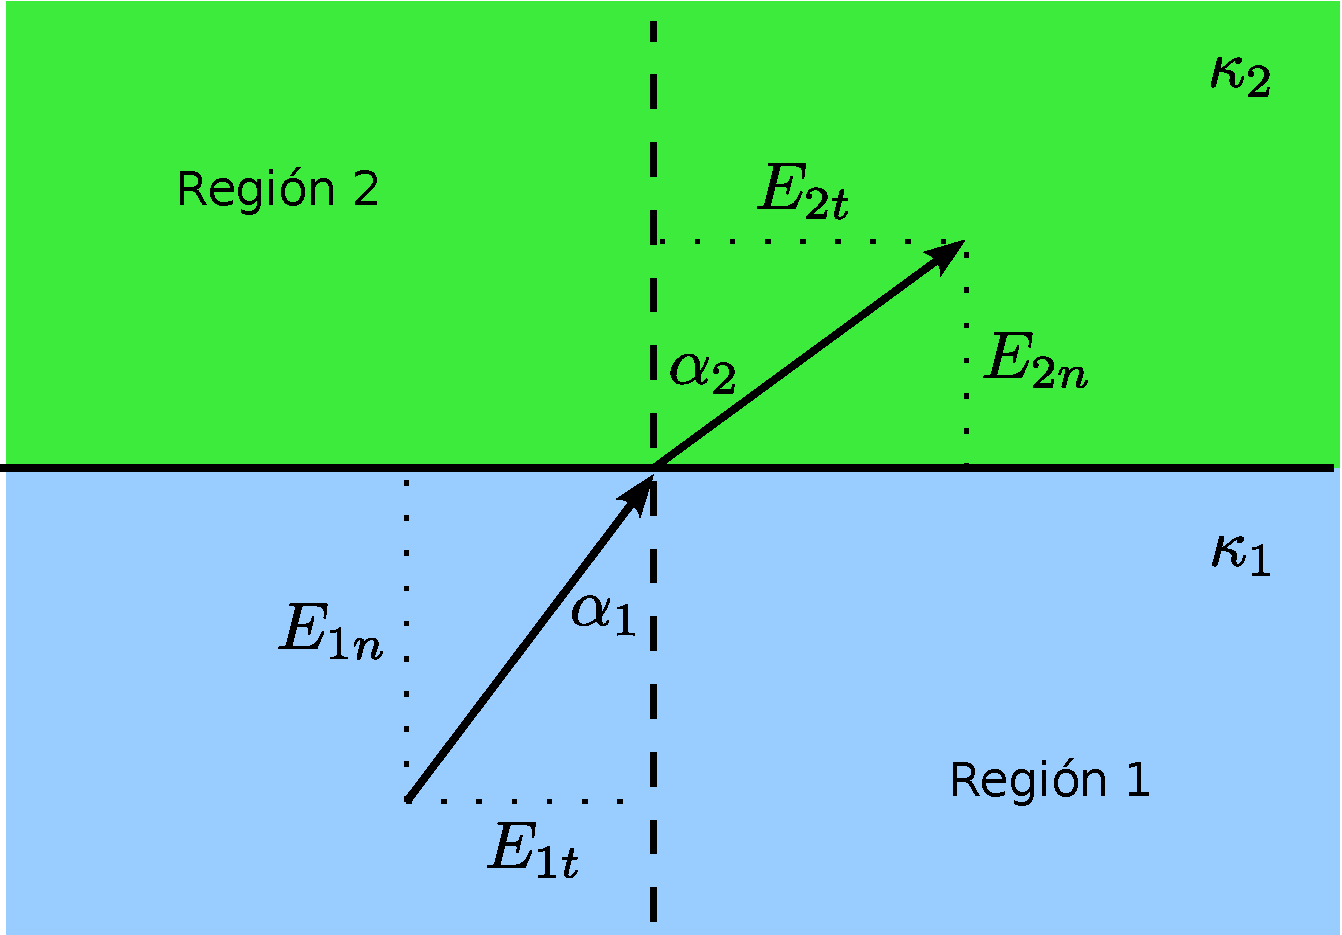
\psfig{file=fig/fig-dielectrico-condicion-borde-03.pdf,height=5cm,
angle=0}}
\caption{Refracci'on de las l'ineas de campo.}
\label{CF3}
\end{figure}
Aqu'i tendremos que, en ausencia de cargas externas, la componente normal del vector desplazamiento es continua a trav'es de la superficie,  $\vec{D}_1\cdot\hat{n}=\vec{D}_2\cdot\hat{n}$, que puede escribirse m'as expl'icitamente como:
\begin{equation}\label{Enid}
\kappa_1 E_1\cos\alpha_1=\kappa_2E_2\cos\alpha_2.
\end{equation}
Por otro lado, la condici'on sobre la componente tangencial a la superficie implica que
\begin{equation} \label{Etid}
 E_1\sin\alpha_1=E_2\sin\alpha_2.
\end{equation}
Dividiendo (\ref{Etid}) por (\ref{Enid}) (asumiendo naturalmente que $E_1$ y $E_2$ son no nulos), obtenemos una simple relaci'on entre los 'angulos $\alpha_1$ y $\alpha_2$:
\begin{equation}
 \frac{\tan\alpha_1}{\kappa_1}=\frac{\tan\alpha_2}{\kappa_2}.
\end{equation}

\subsubsection{Ejemplo: Esf'era diel'ectrica en un campo el'ectrico externo uniforme}
Aqu'i consideraremos el ejemplo de una esfera diel'ectrica (lineal e is'otropa) de radio $R$ y constante diel'ectrica $\kappa_1$ sumergida en un medio de constante diel'ectrica $\kappa_2$ y en presencia de un campo externo constante $\vec{E}_0$.

En este caso no existen cargas externas en el dominio considerado (las 'unicas cargas externas del problema ser'ian aquellas que generan el campo externo, que consideraremos est'an ubicadas muy lejos de la esfera). Entonces el potencial el'ectrico, de acuerdo a (\ref{Poissond}), satisface la ecuaci'on de Laplace tando dentro ($r\le R$) como fuera ($r\ge R$) de la esfera. Resolveremos el problema en coordenadas esf'ericas orientando el eje $z$ en la direcci'on de $\vec{E}_0$. Entonces, debido a la simetr'ia del problema (recuerde que los medios son is'otropos) los campos tendr'an simetr'ia axial. En particular $\phi=\phi(r,\theta)$. Por esto, la forma general del campo en cada regi'on es
 \begin{equation}
 \phi(r,\theta)=\sum_{l=0}^{\infty}\left[  A_lr^{l}+B_lr^{-(l+1)}\right]
 P_l(\cos\theta).
 \end{equation}
En el interior de la esfera el potencial debe ser finito en todo punto y, en particular, en el origen $r=0$. Esta condici'on, junto con la elecci'on $\phi (r=0,\theta)\stackrel{!}{=}0$, reduce la forma posible del potencial a 
 \begin{equation}\label{phiint}
 \phi(r,\theta)=\sum_{l=1}^{\infty}A_l^{(1)}r^{l}P_l(\cos\theta), \qquad r\le R.
 \end{equation}
Por otro lado, lejos de la esfera ($r\gg R$) el campo el'ectrico debe tender al campo el'ectrico externo $\vec{E}_0=E_0\hat{z}$. Esto es equivalente a que el potencial satisfaga
\begin{equation}
 \phi(r,\theta)\to -E_0z+\alpha = -E_0\,r\cos\theta+\alpha, \qquad r\gg R,
\end{equation}
donde $\alpha$ es una constante. Con esta condici'on, el potencial fuera de la esfera s'olo puede adoptar la forma
\begin{equation}\label{phiext}
\phi(r,\theta)=\alpha-E_0\,r\cos\theta+\sum_{l=0}^{\infty}B_l^{(2)}
 r^{-(l+1)}P_l(\cos\theta), \qquad r>R.
\end{equation}
El potencial es una funci'on continua. Por lo tanto, en $r=R$ las soluciones internas y externas deben adoptar el mismo valor. Usando (\ref{phiint}) y (\ref{phiext}) encontramos as'i la condici'on
 \begin{equation}
 \sum_{l=1}^{\infty}A_l^{(1)}R^{l}P_l(\cos\theta)  
 =\alpha-E_0\,R\cos\theta+\sum_{l=0}^{\infty}B_l^{(2)}R^{-(l+1)} P_l(\cos\theta)
 \end{equation}
 que implica, para $l=0$, que
\begin{equation}\label{ecl0a}
\alpha-B_0^{(2)}R^{-1}=0.
\end{equation}
Adem'as, para $l=1$, obtenemos
\begin{equation}\label{ecl1a}
 A_1^{(1)}R =-E_0R+B_1^{(2)}R^{-2}.
\end{equation}
Finalmente, para $l\geq2$, encontramos
\begin{equation}\label{eclla}
 A_l^{(1)}R^{l} =B_l^{(2)}R^{-(l+1)}.
\end{equation}
Por otro lado, la condici'on (\ref{saltoDn}) se reduce, ya que $\sigma_{\rm ext}=0$, a $\vec{D}_1\cdot\hat{n}=\vec{D}_2\cdot\hat{n}$. Adem'as en este caso $\hat{n}=\hat{r}$, por lo que la condici'on es equivalente a
\begin{equation}
\kappa_1\left.\frac{\partial\phi}{\partial r}\right|_{r=R^-}
=\kappa_2\left.\frac{\partial\phi}{\partial r}\right|_{r=R^+}.
\end{equation}
Reemplazano nuevamente (\ref{phiint}) y (\ref{phiext}) en esta condici'on obtenemos
\begin{equation}\label{condD}
 k\sum_{l=1}^{\infty}A_l^{(1)}lR^{l-1}P_l(\cos\theta) =-E_0P_1(\cos\theta)  -\sum_{l=0}^{\infty}(l+1)B_l^{(2)}R^{-(l+2)}P_l(\cos\theta),
\end{equation}
donde hemos definido $k:=\kappa_1/\kappa_2$. Para $l=0$ esta condici'on implica que
\begin{equation}\label{ecl0b}
B_0^{(2)}=0.
\end{equation}
Para el caso $l=1$, obtenemos
\begin{equation}\label{ecl1b}
kA_1^{(1)}  =-E_0-2B_1^{(2)}R^{-3}.
\end{equation}
Finalmente, para $l\geq2$, encontramos la condici'on
\begin{equation}\label{ecllb}
klA_l^{(1)} =-(l+1)B_l^{(2)}R^{-(2l+1)}.
\end{equation}
Al reemplazar el resultado (\ref{ecl0b}) en (\ref{ecl0a}) obtenemos $\alpha=0$. Similarmente, las ecuaciones (\ref{ecl1a}) y (\ref{ecl1b}) permiten encontrar las constantes $A_1^{(1)}$ y $B_1^{(2)}$. Simple 'algebra muestra que la soluci'on en este caso es dada por
\begin{equation}
 A_1^{(1)}=\frac{-3}{k+2}E_0, \qquad, B_1^{(2)}=\frac{k-1}{k+2}R^3E_0.
 \end{equation}
Finalmente, las ecuaciones (\ref{eclla}) y (\ref{ecllb}) determinan $A_l^{(1)}$ y $B_l^{(2)}$ para $l\ge 2$. En este caso, sin embargo, la 'unica soluci'on posible es la nula, es decir,
\begin{equation}
A_l^{(1)}=0, \qquad B_l^{(2)}=0, \qquad l\ge 2.
\end{equation}
Con esto, la soluci'on para el potencial queda totalmente determinado tanto dentro como fuera de la esfera:
\begin{equation}
\phi(r,\theta)=\frac{-3\kappa_2}{\kappa_1+2\kappa_2}E_0\,r\cos\theta, \qquad r\le R
\end{equation}
y
\begin{equation}
\phi(r,\theta)=-E_0\,r\cos\theta +\frac{\kappa_1-\kappa_2}{\kappa_1+2\kappa_2}R^3E_0 \frac{\cos\theta}{r^2}, \qquad r\ge R.
\end{equation}
 
 Ahora estudiaremos algunas caracter'isticas de la soluci'on obtenida, en el caso particular en que fuera de la esfera hay s'olo vac'io, es decir, $\kappa_2=1$. Primero, el potencial en el interior de la esfera puede escribirse, en coordenadas cartesianas como
 \begin{equation}
\phi(r,\theta)=\frac{-3}{\kappa_1+2}E_0\,z, \qquad r\le R,
\end{equation}
lo que implica que el campo el'ectrico en el interior de la esfera es homog'eneo y dado por
\begin{equation}
\vec{E}=\frac{3}{\kappa_1+2}\,\vec{E}_0, \qquad r\le R.
\end{equation}
% Adem'as,%
% \begin{equation}
% E_{r}^{(2)}=-\frac{\partial\phi^{(2)}}{\partial r}=E^0r\cos\theta
% +2\frac{k_1-k_2}{k_1+2k_2}a^3E^0r^{-2}\cos\theta
% \end{equation}%
% \begin{equation}
% E_{\theta}^{(2)}=-\frac{1}{r}\frac{\partial\phi^{(2)}}{\partial\theta
% }=-E^0r\sen\theta+\frac{k_1-k_2}{k_1+2k_2}a^3E^0r^{-2}%
% \sen\theta
% \end{equation}%
% \begin{equation}
% E_{\varphi}^{(2)}=0
% \end{equation}

Por otro lado, fuera de la esfera, el potencial consta de dos t'erminos: uno que corresponde al campo homog'eneo externo y otro con la forma (es decir, dependencia espacial) de un \textit{campo dipolar}. En efecto, el campo de un dipolo el'ectrico con momento dipolar $\vec{p}=p\hat{z}$ orientado a lo largo del eje $z$ es
 \begin{equation}
 \phi_{\rm dip}=\frac{p}{4\pi\varepsilon_0}\frac{\cos\theta}{r^2}.
 \end{equation}
Por lo tanto, el campo en el exterior de la esfera diel'ectrica es dado por la suma del campo externo$\vec{E}_0$ y el campo de un dipolo con momento dipolar
 \begin{equation}
\vec{p}=4\pi\varepsilon_0\frac{\kappa_1-1}{\kappa_1+2}R^3\,\vec{E}_0.
 \end{equation}
Puede verficarse que esta identificaci'on es correcta recordando que el vector de polarizaci'on es definido como la densidad de momento dipolar del medio. Como consecuencia, la relaci'on (\ref{pintPdV}) permite calcular el momento dipolar total de la esfera como una integral de volumen de su vector de polarizaci'on. En el caso estudiado, el vector de polarizaci'on es proporcional al campo el'ectrico y por lo tanto tambi'en homog'eneo al interior de la esfera:
\begin{align}
\vec{P} &= \varepsilon_0(\kappa_1-1)\vec{E} \\
&= \frac{3\varepsilon_0(\kappa_1-1)}{\kappa_1+2}\,\vec{E}_0.
\end{align}
Con esto, el momento dipolar de la esfera puede ser calculado f'acilmente:
\begin{align}
\vec{p} &= \int_V \vec{P}\,dV \\
&= \vec{P}\,V \\
&= \frac{3\varepsilon_0(\kappa_1-1)}{\kappa_1+2}\,\vec{E}_0\cdot \frac{4\pi}{3}R^3.
\end{align}
Finalmente, podemos calcular las densidades de carga de polarizaci'on en la esfera. Ya que el vector de polarizaci'on es homog'eneo, la densidad $\rho_P=0$. La densidad superficial de carga de polarizaci'on $\sigma_P$ es no nula:
\begin{align}
\sigma_P &= \vec{P}\cdot\hat{r}\\
&= \frac{3\varepsilon_0(\kappa_1-1)}{\kappa_1+2}\,E_0\,\cos\theta.
\end{align}

Finalmente, es interesante notar que el caso de un \textit{conductor} esf'erico de carga total nula, en un campo externo homog'eneo, ver secci'on \ref{sec:esfcond}, puede ser recobrado en el l'imite $\kappa_1\to\infty$.

\subsection{Modelos microsc'opicos simples de polarizaci'on}
\subsubsection{Polarizalibidad}
En muchos casos, los 'atomos que constituyen un diel'ectrico no est'an polarizados...

\subsection{Energ'ia electrost'atica en un diel'ectrico}

En la secci'on \ref{ed3_1_2} vimos una expresi'on para la energ'ia almacenada
en un campo dado o, equivalentemente la energ'ia necesaria para formar el
sistema de cargas correspondientes a un campo. Ahora calcularemos algo
an'alogo, pero diferente: la energ'ia almacenada en una configuraci'on de campo
en un sistema que consta de cargas externas y un diel'ectrico \underline{dado}.
En otras palabras, \textit{no incluiremos la energ'ia necesaria para formar el
diel'ectrico}, sino s'olo la energ'ia necesaria para montar una cierta
distribuci'on de cargas externas en un diel'ectrico preexistente.

El trabajo necesario para aumentar (en general, para cambiar) la densidad de
cargas externas en $\delta\rho_{\rm ext}(x)$ en un medio con potencial
$\phi(x)$ es dado por
\begin{equation}\label{Wdiel1}
 \boxed{\delta U=\int_{R^3}\phi(x)\delta\rho_{\rm ext}(x)\,dV.} 
\end{equation}
Usando (\ref{divD}) encontramos que el cambio en densidad de cargas externas
est'a relacionado con el cambio en el vector desplazamiento por medio de
$\vec\nabla\cdot(\delta\vec{D})=\delta\rho_{\rm ext}$. Usando esto, e integrando
por partes, podemos reescribir (\ref{Wdiel1}) como:
\begin{equation}
 \delta U=\oint_{\infty}\phi (x)\delta\vec{D}(x)\cdot
d\vec{S}+\int_{R^3}\vec{E}\cdot\delta\vec{D}\,dV.
\end{equation}
Asumiendo, como es usual, que los campos se anulan suficientemente r'apido en
el infinito, llegamos a
\begin{equation}
 \boxed{\delta U=\int_{R^3}\vec{E}(x)\cdot\delta\vec{D}(x)\,dV.} \label{dUE}
\end{equation}
Si las cargas externas est'an posicionadas de forma tal que (en cada punto) su
densidad es una fracci'on $\lambda$ de la densidad final, es decir, si es
$\lambda\rho_{\rm ext}(x)$, entonces el vector desplazamiento correspondiente
ser'a $\lambda\vec{D}(x)$ (como consecuencia de (\ref{divD})) y el campo
el'ectrico correspondiente lo denotaremos $\vec{E}_\lambda(x)$. Al incrementar
ahora la densidad en $\delta\rho_{\rm ext}(x)=\rho_{\rm ext}(x)\,d\lambda$ el cambio respectivo del vector desplazamiento es $\delta\vec{D}(x)=\vec{D}(x)\,d\lambda$. Entonces, la energ'ia total requerida para ``montar'' una distribuci'on de carga (final)
$\rho_{\rm ext}(x)$ o, equivalentemente, la energ'ia necesaria para que el campo
el'ectrico sea $\vec{E}(x)$ y el vector desplazamiento $\vec{D}(x)$ puede
calcularse ``sumando''\, las energ'ias necesarias en cada incremento, desde la
situaci'on inicial donde no hay cargas externas ($\lambda=0$) hasta alcanzar el
100\% de las cargas y campos ($\lambda=1$):
\begin{equation}
U=\int_0^1 d\lambda\int_{R^3}\vec{E}_\lambda\cdot \vec{D}\,dV .
\end{equation}
Esta expresi'on es v'alida en general, para cualquier tipo de diel'ectrico.

Para \textit{medios lineales} las componentes del vector desplazamiento son directamente proporcionales a las componentes del campo el'ectrico, luego $\vec{E}_\lambda(x)=\lambda\vec{E}(x)$.
En este caso, la energ'ia necesaria para obtener, en un medio diel'ectrico lineal preexistente, una cierta configuraci'on de campos y cargas es 
\begin{equation}\marginnote{Energ'ia medios lineales}
\boxed{U=\frac{1}{2}\int_{R^3}\vec{E}\cdot\vec{D}\,dV.} \label{UED}
\end{equation}
La respectiva \textit{densidad de energ'ia} electrost'atica asociada es, entonces,
\begin{equation}
\boxed{u(x)=\frac{1}{2}\,\vec{E}(x)\cdot\vec{D}(x).}
\end{equation}
En general, para un medio anis'otropo tendremos
\begin{equation}
u(x)=\frac{\varepsilon_0}{2}\,\kappa_{ij}(x)E_i(x)E_j(x).
\end{equation}
Finalmente, para un medio is'otropo
\begin{equation}\marginnote{Energ'ia medios is'otropos}
\boxed{u=\frac{\varepsilon_0}{2}\,\kappa\,\vec{E}^2.}
\end{equation}

Note finalmente que, en t'erminos del potencial y la densidad de carga externa, la energ'ia (\ref{UED}) puede escribirse como:
\begin{equation}
U=\frac{1}{2}\int_{R^3}\phi(x)\rho_{\rm ext}(x)\,dV.
\end{equation}

\subsection{Fuerzas y torques}
El conocimiento de la energ'ia electrost'atica de sistemas que constan de
cargas, conductores y diel'ectricos puede ser usada para calcular
(generalmente en forma simple) fuerzas y torques actu'ando sobre una parte del
sistema. Para esto, deben considerarse dos subcasos: a) aquellos sistemas que
est'an aislados y, por lo tanto, la carga y la energ'ia total del sistema son
constantes, y b) sistemas que no est'an aislados, pero en los que, fuentes
(bater'ias) externas mantienen constante las diferencias de potencial entre los conductores
presentes.

\subsubsection{Sistema aislado}

En este caso, el trabajo $\delta W$ realizado por las fuerzas que act'uan sobre una de
las \textit{partes m'oviles} del sistema debe producirse a costa de la
variaci'on de la energ'ia electrost'atica del mismo sistema, $\delta U$, es decir,
\begin{equation}
 \delta W + \delta U=0. \label{dW+dU=0}
\end{equation}
Si la parte m'ovil realiza un desplazamiento (real o virtual) $\delta x_i$ a
partir de su posici'on inicial $x_i$, y la fuerza sobre ella es $F_i$ entonces
\begin{equation}
 \delta W=F_i\,\delta x_i. \label{trab}
\end{equation}
Usando (\ref{dW+dU=0}) y (\ref{trab}) podemos entonces escribir
\begin{equation}\marginnote{Fuerza Sistema Aislado}
\boxed{F_i=-\left(\frac{\partial U}{\partial x_i}\right)_Q ,} \label{FQ}
\end{equation}
donde el sub'indice $Q$ indica que al efectuar las derivadas parciales debe
tenerse en cuenta que la carga del sistema se mantiene constante, y la energ'ia
electrost'atica debe ser escrita en funci'on de la posici'on de la parte
m'ovil, $U=U(x_i)$.

En el caso que la parte m'ovil \textit{rota en un 'angulo $\delta\theta$ respecto a un eje determinado por el vector $\hat{n}$}, tenemos que $\delta W=\hat{\tau}\cdot\hat{n}\delta\theta$, de modo que \textit{el torque
sobre la parte m'ovil} puede ser calculado usando
\begin{equation}\label{torqueU}\marginnote{Torque Sistema Aislado}
 \boxed{\vec{\tau}\cdot\hat{n}=-\left(\frac{\partial U}{\partial\theta}\right)_Q
.}
\end{equation}
An'alogamente al caso ``traslacional'' de la fuerza, la expresi'on \eqref{torqueU} asume que se ha determinado la dependencia de la energ'ia electrost'atica del sistema en funci'on del la posici'on angular de la parte m'ovil, es decir, que se conoce la funci'on $U(\theta)$.


\subsubsection{Sistema con conductores a potencial constante}

En este caso, el trabajo realizado por las fuerzas que act'uan sobre una de
las partes m'oviles del sistema, m'as la variaci'on de la energ'ia
electrost'atica del sistema, debe ser igual a la energ'ia suministrada por las
bater'ias que mantienen los conductores a potenciales constantes, $\delta
W_{\rm b}$, de modo que
\begin{equation}
 \delta W + \delta U=\delta W_{\rm b}. \label{dW+dU=dWb}
\end{equation}
Ahora, la variaci'on de la energ'ia electrost'atica de los conductores con
potenciales fijos es dada, ver \eqref{Wdiel1}, por
\begin{equation}
 \delta U=\frac{1}{2}\sum_{(\alpha)}\phi^{(\alpha)}\delta Q^{(\alpha)},
\end{equation}
donde $\delta Q^{(\alpha)}$ es el cambio de las cargas en el conductor $\alpha$-'esimo,
necesaria para mantener su potencial $\phi^{(\alpha)}$ constante. Por otro lado, 
la energ'ia suministrada por las bater'ias es igual al trabajo necesario para
transportar las cargas $\delta Q^{(\alpha)}$ hasta cada conductor, es decir,
\begin{equation}
 \delta W_{\rm b}=\sum_{(\alpha)}\phi^{(\alpha)}\delta Q^{(\alpha)}.
\end{equation}
De esta forma encontramos que
\begin{equation}
 \delta W_{\rm b}=2\delta U.
\end{equation}
Con este resultado y (\ref{dW+dU=dWb}) llegamos a
\begin{equation}
 \delta U=\delta W,
\end{equation}
que, en los casos de desplazamientos y rotaciones, implica
\begin{equation}
\boxed{F_i=\left(\frac{\partial U}{\partial x_i}\right)_\phi ,}
\end{equation}
y, para el torque,
\begin{equation}
 \boxed{\vec{\tau}\cdot\hat{n}=\left(\frac{\partial
U}{\partial\theta}\right)_\phi
.}
\end{equation}

\subsubsection{Ejemplo: Fuerza sobre un condensador semi-lleno con un
diel'ectrico}
\begin{figure}[!h]
\centerline{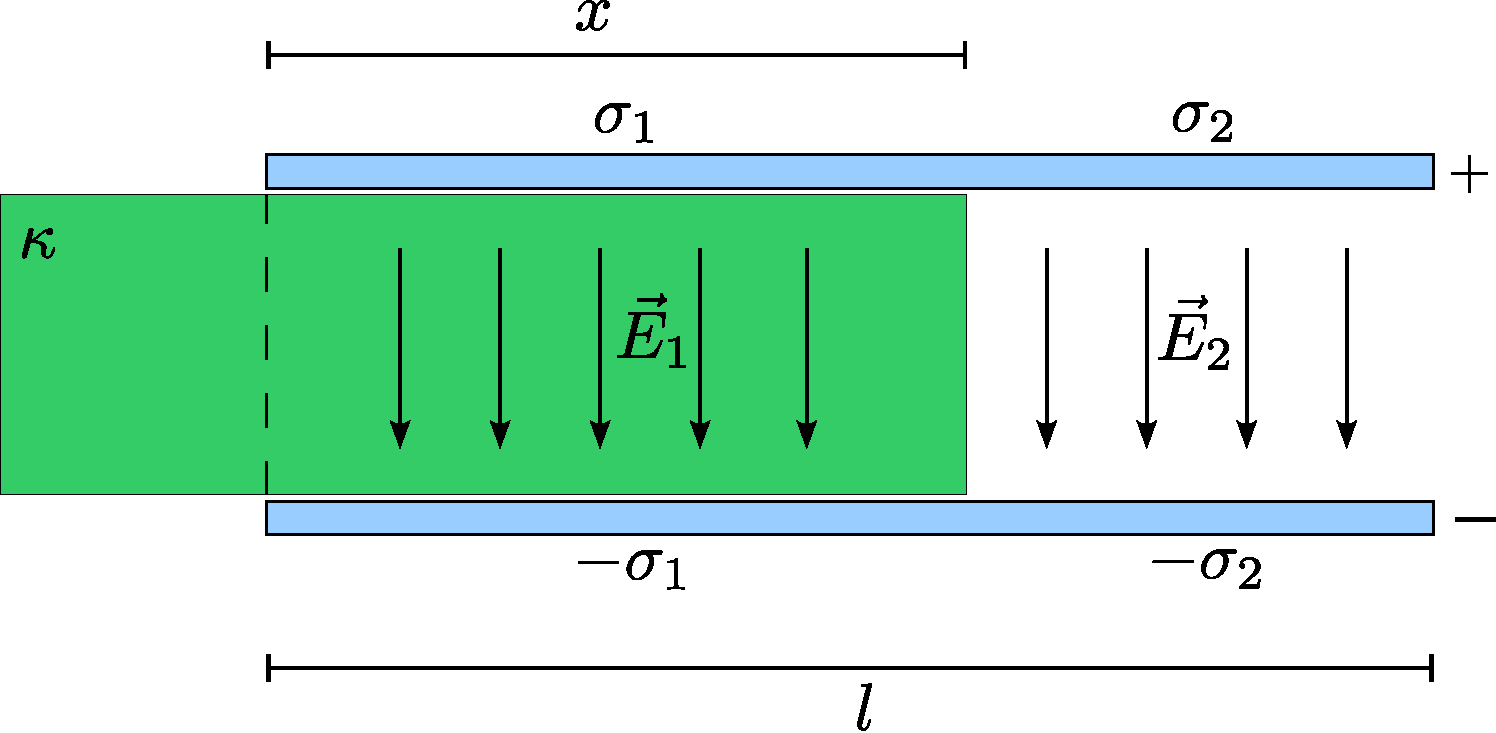
\psfig{file=fig/fig-condensador-semi-lleno-01.pdf , height=4cm ,
angle=0}}
\caption{Condensador parcialmente lleno con diel'ectrico.}
\label{fig:fccd}
\end{figure}
Consideremos el caso en que el sistema est'a cargado, con cargas $+Q$ y $-Q$
respectivamente, y aislado. Debemos determinar los campos en la regi'on con
diel'ectrico (regi'on 1) y sin 'el (regi'on 2). Despreciando efectos de borde,
podemos aproximar que todos los campos son verticales, con sus sentidos hacia
abajo en la figura. Ya que la componente tangencial del campo el'ectrico es
continua en una interfase entre dos diel'ectricos, encontramos que el campo
el'ectrico $\vec{E}$ es igual en todo punto entre las placas del condensador,
es decir,
\begin{equation}
 E_1=E_2.
\end{equation}
Usando (\ref{GaussD}) encontramos directamente que
\begin{equation}
 D_1=\varepsilon_0\kappa E=\sigma_1, \qquad D_2=\varepsilon_0 E=\sigma_2,
\end{equation}
donde $\sigma_1$ y $\sigma_2$ son las densidades de carga en las placas en la
regi'on correspondiente. La carga total en cada placa es entonces dada por
\begin{eqnarray}
 Q&=&\sigma_1A_1+\sigma_2A_2 \\
&=& \varepsilon_0\kappa E w x+\varepsilon_0E w (l-x) \\
&=& \varepsilon_0Ew\left(\kappa x+l-x\right), \label{Qej}
\end{eqnarray}
donde $w$ es la longitud de la otra arista del rect'angulo que define cada placa (es decir, en la direcci'on perpendicular a la figura \ref{fig:fccd}).

La energ'ia electrost'atica del sistema puede ser calculada evaluando
(\ref{UED}):
\begin{eqnarray}
 U&=&\frac{1}{2}\int\vec{D}\cdot\vec{E}\,dV \\
&=&\frac{1}{2}\left(D_1EV_1+D_2EV_2\right) \\
&=&\frac{1}{2}\left[\varepsilon_0\kappa
xwd+\varepsilon_0(l-x)wd\right]E^2 \\
&=&\frac{1}{2}\varepsilon_0\left(\kappa x+l-x\right)wdE^2 .
\end{eqnarray}
Usando (\ref{Qej}), podemos finalmente expresar la energ'ia electrost'atica
del sistema como
\begin{equation}
U(x)=\frac{Q^2d}{2\varepsilon_0 w}\frac{1}{(\kappa x+l-x)}.
\end{equation}
Ya que el sistema est'a aislado y $Q$ es constante, la fuerza sobre el
diel'ectrico puede ser calculada a partir de (\ref{FQ}). As'i obtenemos
\begin{equation}
 F(x)=\frac{Q^2d}{2\varepsilon_0 w}\frac{(\kappa-1)}{(\kappa x+l-x)^2},
\end{equation}
que es una fuerza que \textit{atrae al diel'ectrico hacia el interior de las
placas}.

\subsubsection{Ejemplo: Electr'ometro}
\newpage
\chapter{Magnetoest'atica}


\section{Corriente y densidad de corriente}

Cuando existen cargas en movimiento, se define la \textit{corriente el'ectrica} $I$ como
la cantidad de \textit{carga neta} que pasa por unidad de tiempo a trav'es de una superficie $S$ \textit{en una direcci'on determinada}, 
\begin{equation}\marginnote{Corriente el'ectrica}
I(t) :=\lim_{\Delta t\to 0}\frac{\Delta Q}{\Delta t}=\frac{dQ}{dt},
\end{equation}
de modo que la carga neta que atraviesa entre los tiempos $t_1$ y $t_2$ una superficie por donde circula una corriente $I(t)$ es
\begin{equation}
Q=\int_{t_1}^{t_2}I(t)\,dt.
\end{equation}
La unidad S.I. para la corriente es el \textbf{Amp\`ere}: $1A:=1C/1s$.

\subsection{Densidad de Corriente}

Consideremos una superficie sobre la cual inciden cargas con densidad $\rho$,
movi'endose con velocidad $\vec{v}$, cruzando un elemento de superficie (orientado) $d\vec{S}$.
\begin{figure}[!h]
\centerline{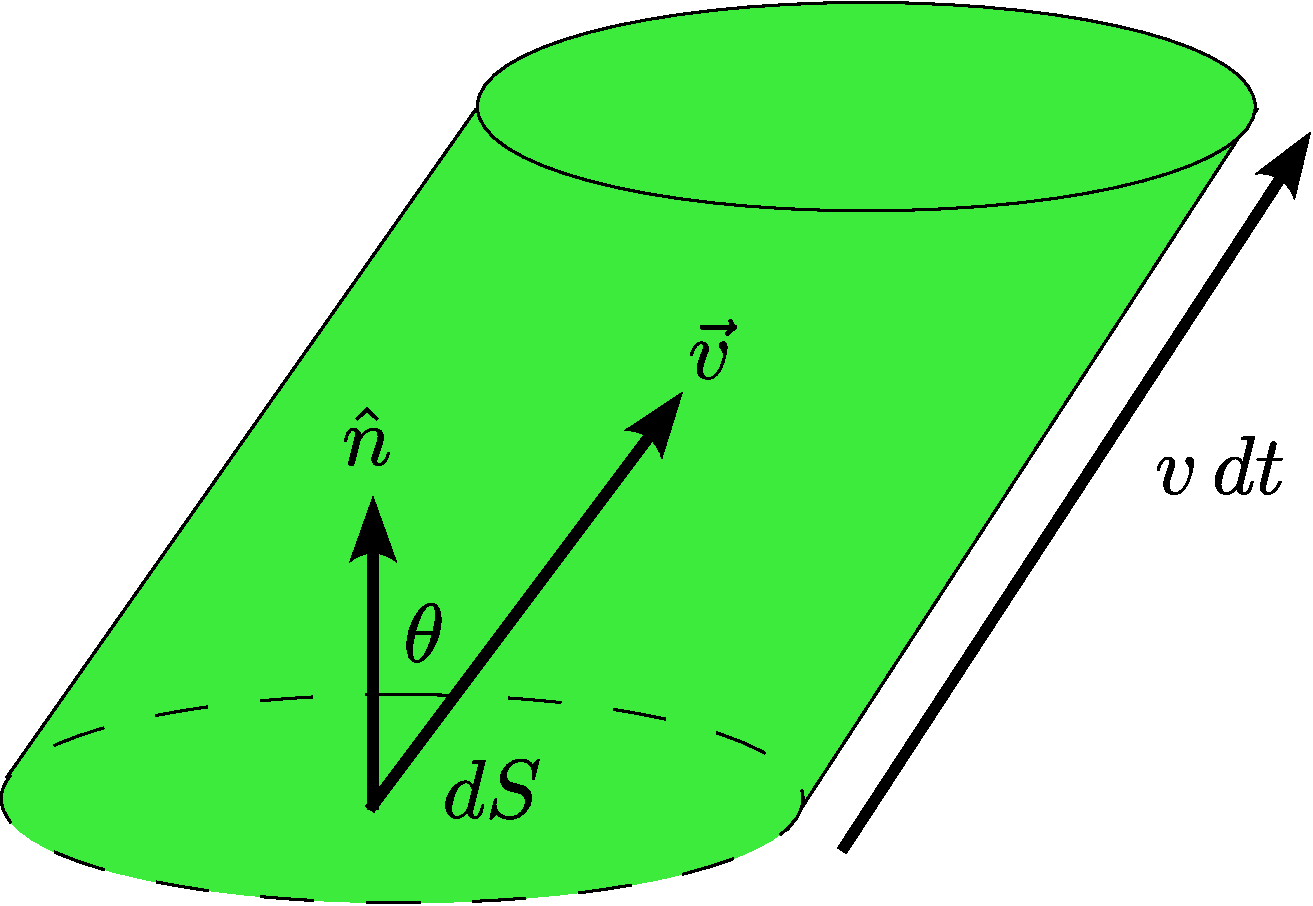
\psfig{file=fig/fig-flujo-cargas-01.pdf,height=4cm,angle=0}}
\caption{Carga con densidad $\rho$ flujendo con velocidad $\vec{v}$ a trav'es
de un elemento de superficie $d\vec{S}$.}
\label{MD1}
\end{figure}
La carga neta que atraviesa el 'area $dS$ en un intervalo de tiempo $dt$ es la que
est'a contenida en un cilindro oblicuo de base $dS$ y de largo $v\,dt$. Ver
figura \ref{MD1}.

Esto permite escribir:
\begin{equation}
dQ=\rho\, dV=\rho\, dS\,(v\,dt)\cos\theta=\rho\,\vec{v}\cdot d\vec{S}\,dt.
\end{equation}
Definimos la \textbf{densidad de corriente}
\begin{equation}\marginnote{Densidad de Corriente}
\boxed{\vec{J}(x):=\rho(x)\vec{v}(x),}
\end{equation}
de modo que
\begin{equation}
 dQ=\vec{J}\cdot d\vec{S}\,dt .
\end{equation}
En otras palabras, la densidad de corriente es la carga por unidad de tiempo y
por unidad de superficie que atraviesa un elemento de 'area normal dado.
Como consecuencia, la corriente, es decir, la carga por unidad de tiempo,
que atraviesa una superficie $S$ es dada por
\begin{equation}
I=\int_{S}\vec{J}\cdot d\vec{S}.
\end{equation}
Es importante notar que si $\rho>0$, entonces $\vec{J}$ y $\vec{v}$ tienen igual
sentido, mientras que si $\rho<0$, entonces $\vec{J}$ y $\vec{v}$ tienen
sentidos opuestos.

\section{Conservaci'on de la carga el'ectrica}

La ley (experimental) de conservaci'on (local) de la carga el'ectrica puede ser escrita
en general, como
\begin{equation}
\frac{d{\ }}{dt}\int_V \rho\,dV=-\int_{\partial V}\vec{J}\cdot d\vec{S},
\end{equation}
que expresa el hecho que todo cambio en la carga neta contenida en un volumen $V$ dado (pero arbitrario) es debido al flujo neto de carga por la superficie ${\partial V}$ que lo encierra. Usando el teorema de Gauss, podemos transformar la integral de superficie a una integral de volumen, obteniendo
\begin{equation}
\int_V\left(\frac{\partial\rho}{\partial t}+\vec{\nabla}\cdot\vec{J}\right)\,dV
 =0.
\end{equation}
Como esta relaci'on debe ser v'alida para todo volumen $V$, es decir, de tama\~no y forma arbitraria, es necesario que
\begin{equation}\marginnote{Conservaci'on local carga}
\boxed{\frac{\partial\rho}{\partial t}
+\vec{\nabla}\cdot\vec{J}=0.}\label{eccont}
\end{equation}
Esta relaci'on es conocida como la \textit{ecuaci'on de continuidad}.

\subsection{Corrientes Estacionarias}

Un caso de particular inter'es es aquel en que las corrientes son
\textit{estacionarias}, es decir, en las que tanto $\rho$ como $\vec{J}$ \textit{no dependen del tiempo}. Bajo estas condiciones, la ecuaci'on de continuidad requiere que la
divergencia de la densidad de corriente sea nula:
\begin{equation}\marginnote{Caso estacionario}
 \vec{\nabla}\cdot\vec{J}=0. \label{divJ0}
\end{equation}


% \subsection{Modelo de Conductividad}
%
% Suponemos que los electrones se mueven en la red at'omica. La ecuaci'on
% de movimiento es
% \begin{equation}
% mn\frac{du_i}{dt} -nqE_i=F_i%
% \label{magstatica-mov}%
% \end{equation}
% donde $T$ es la temperatura del gas de electrones, y $F_i=-mn\nu u_i$ es
% la fuerza debido a las colisiones. Recordando que $\rho=nq$ y que
% $j_i=nqu_i$ tenemos que en la ecuaci'on (\ref{eccont} )
% resulta%
% \begin{equation}
% \frac{\partial\rho}{\partial t}+\partial_i\left(  \rho u_i\right)  =0
% \end{equation}
% de la ecuaci'on (\ref{magstatica-mov}) y suponiendo que el gradiente de
% temperatura es despreciable, tenemos%
% \begin{align*}
% mn\frac{du_i}{dt}-nqE_i  & =-mn\nu u_i\\
% n\frac{d\left(  u_i\right)  }{dt}  & =\frac{nq}{m}E_i-\nu u_i%
% \qquad\qquad/\cdot q\\
% \frac{d\left(  nqu_i\right)  }{dt}  & =\frac{nq^2}{m}E_i-\nu nqu_i\\
% \frac{dj_i}{dt}+\nu j_i  & =\frac{nq^2}{m}E_i%
% \end{align*}
% Si $\vec{J}$ es constante en el tiempo%
% \begin{equation}
% j_i=\frac{nq^2}{m\nu}E_i=\sigma E_i%
% \end{equation}
% llamando a $\sigma$ conductividad el'ectrica. Notar que la conductividad es
% inverso a la resistencia el'ectrica, es decir, $\sigma=1/R~~\left[
% 1/\Omega\right]  $

% \subsubsection{Aplicaci'on: Velocidad de distribuci'on de la carga}
%
% Velocidad con que se distribuye la carga el'ectrica en un conductor con
% conductividad $\sigma$. Veamos que,%
% \begin{equation}
% j_i=\sigma E_i%
% \end{equation}
% luego en la euaci'on de continuidad (\ref{eccont} ) tenemos%
% \begin{align*}
% \frac{\partial\rho}{\partial t}+\vec{\nabla}\cdot\vec{J}  & =0\\
% \frac{\partial\rho}{\partial t}+\sigma\partial_iE_i  & =0\\
% \frac{\partial\rho}{\partial t}+\frac{\sigma}{\varepsilon_0}\rho & =0
% \end{align*}
% Esta ecuaci'on diferencial tiene como soluci'on%
% \begin{equation}
% \rho(t)=\rho_0~e^{-t/t_0}%
% \end{equation}
% donde $t_0=\varepsilon_0/\sigma$. Para valores experimentales tenemos que
% $\varepsilon_0=8.8512\times10^{-12}~\left[  c^2/Nm^2\right]  $ y para el
% cobre se tiene que $\sigma=59.88~\left[  1/\Omega\right]  $ luego conociendo
% la densidad del cobre podemos saber como varia la densidad de carga en el
% tiempo para un volumen dado.

\section{Campo magn'etico y fuerza magn'etica}
Se ha encontrado \textit{experimentalmente} que la fuerza que act'ua sobre una peque\~na carga $q$, movi'endose con velocidad $\vec{v}$ en un campo magn'etico dado es proporcional a $q$, a la rapidez $v$, y que tiene direcci'on perpendicular a $\vec{v}$. Esto permite \textit{definir}  la \textit{intensidad de campo magn'etico} $\vec{B}$ como un (pseudo-)vector tal que (en el sistema internacional de unidades)
\begin{equation}
 \vec{F}_{\rm m}=q\,\vec{v}\times\vec{B}.
\end{equation}
Por lo tanto, la fuerza total que act'ua sobre una carga $q$ en un punto del espacio con campo el'ectrico $\vec{E}$ y magn'etico $\vec{B}$ es dada por la \textit{fuerza de Lorentz}\footnote{En honor a Hendrik Antoon Lorentz (1853-1928): f'isico y matem'atico holand'es. Ganador del Premio Nobel de F'isica en 1902. Ver \url{http://es.wikipedia.org/wiki/Hendrik_Lorentz}.}
\begin{equation}\marginnote{Fuerza de Lorentz}
\boxed{ \vec{F}=q\left(\vec{E}+\vec{v}\times\vec{B}\right).}
\end{equation}
La unidad de medida de la intensidad de campo magn'etico $\vec{B}$ es entonces  $[B]=Ns/Cm=Vs/m^2$ , que se define como un \textit{Tesla}: $1T:=Vs/m^2$. Alternativamente se define un
\textit{Gauss} como $1G:=10^{-4}T$. \footnote{Por ejemplo, la magnitud campo
magn'etico interestelar oscila entre $0,1$ and $10$ $nT$, el campo magn'etico
de la Tierra es de orden $\approx 0,5 G$, mientras que un im'an
de Neodimio (Nd${}_2$Fe${}_{14}$B) produce un campo del orden de $1.25\, T$.
Un magneto de un sistema de resonancia magn'etica produce campos entre $1,5\,T$
y $3\,T$. Los campos magn'eticos m'as intensos producidos en un laboratorio son
del orden de $100\,T$ \cite{MagLab2012,HZDR2011}. El campo magn'etico en una estrella de neutrones puede oscilar entre 1 y 100 MT.}

Como consecuencia directa del hecho que la fuerza magn'etica es perpendicular a
la velocidad de las cargas, \textit{el campo magn'etico no realiza trabajo} sobre ellas.
Esto tiene como consecuencia que el campo magn'etico s'olo puede cambiar la
direcci'on de la velocidad de una carga y no su m'odulo (energ'ia cin'etica).

Si las cargas est'an distribuidas continuamente, entonces la fuerza magn'etica total sobre una regi'on $V$ con densidad $\rho$ y velocidad $\vec{v}$ ser'a
\begin{equation}\marginnote{Fuerza magn'etica}
 \vec{F}_{\rm m}=\int_V
\rho\vec{v}\times\vec{B}\,dV=\int_V\vec{J}\times\vec{B}\,dV. \label{fm1}
\end{equation}
Podemos describir esta situaci'on usando la \textbf{densidad de fuerza
magn'etica} $\vec{f}_{\rm m}$, definida como la fuerza por unidad de volumen,
dada por
\begin{equation}
 \vec{f}_{\rm m}:=\vec{J}\times\vec{B},
\end{equation}
de modo que
 \begin{equation}
\vec{F}_{\rm m}=\int_V\vec{f}_{\rm m}\,dV. \label{dfm}
\end{equation}


% \subsection{Trayectorias en un campo el'ectromagn'etico}
% Usando () y la segunda ley de Newton, tenemos
% \begin{equation}
% m\frac{dv_i}{dt}=qE_i+q\varepsilon_{ijk}v_jB_k
% \end{equation}
% Multiplicando esta ecuaci'on con $v_i$, obtenemos
% \begin{equation}
%  \frac{d\ }{dt}(\frac{m}{2}v^2)=qv_iE_i
% \end{equation}
% \begin{equation}
%  \frac{dK}{dt}=qv_iE_i
% \end{equation}
% S'olo el campo el'ectrico realiza trabajo sobre la carga, modificando su
% energ'ia ci'n'etica.
% \begin{equation}
%  dK=qv_iE_idt=qE_idx_i=-q\partial_i\phi dx_i=-qd\phi
% \end{equation}
% \begin{equation}
%  d(K+q\phi)=0
% \end{equation}
% \begin{equation}
%  \frac{1}{2}mv^2+q\phi={\rm cte}
% \end{equation}
% a lo largo de la trayectoria.


\section{Ley de Biot-Savart}
Biot\footnote{Jean Baptiste Biot: F'isico, Astr'onomo y Matem'atico franc'es (1774-1862). Ver \url{http://es.wikipedia.org/wiki/Jean_Baptiste_Biot}.} y Savart\footnote{F'elix Savart: F'isico, M'edico y Profesor franc'es (1791-1841). Ver \url{http://es.wikipedia.org/wiki/F\%C3\%A9lix_Savart}.} encontraron ($\sim$\,1820) que el campo magn'etico $d\vec{B}$ que un peque\~no segmento $dx'$ orientado en la direcci'on de flujo de la corriente $I$ y ubicado en la posici'on $\vec{x}'$ produce en un punto de posici'on $\vec{x}$ es proporcional a la intensidad de corriente, al largo del
peque\~no segmento, e inversamente proporcional al cuadrado de la distancia
entre el segmento y el punto de observaci'on, es decir,
\begin{equation}
 \left\vert d\vec{B}\right\vert \propto
\left(I,dx',\frac{1}{\left|\vec{x}-\vec{x}'\right|^2}\right),
\end{equation}
y que la direcci'on del campo producido es perpendicular a $d\vec{x}'$ y al
vector que une el segmento con el punto de observaci'on,
\begin{equation}
d\vec{B}  \perp\left(  d\vec{x}', \vec{x}-\vec{x}' \right) ,
\end{equation}
y que, finalmente, el sentido del campo magn'etico es dado por la regla de la mano derecha a partir de los vectores $d\vec{x}'$ y $\vec{x}-\vec{x}'$. Ver figura \ref{fBS1}. 
\begin{figure}[!h]
\centerline{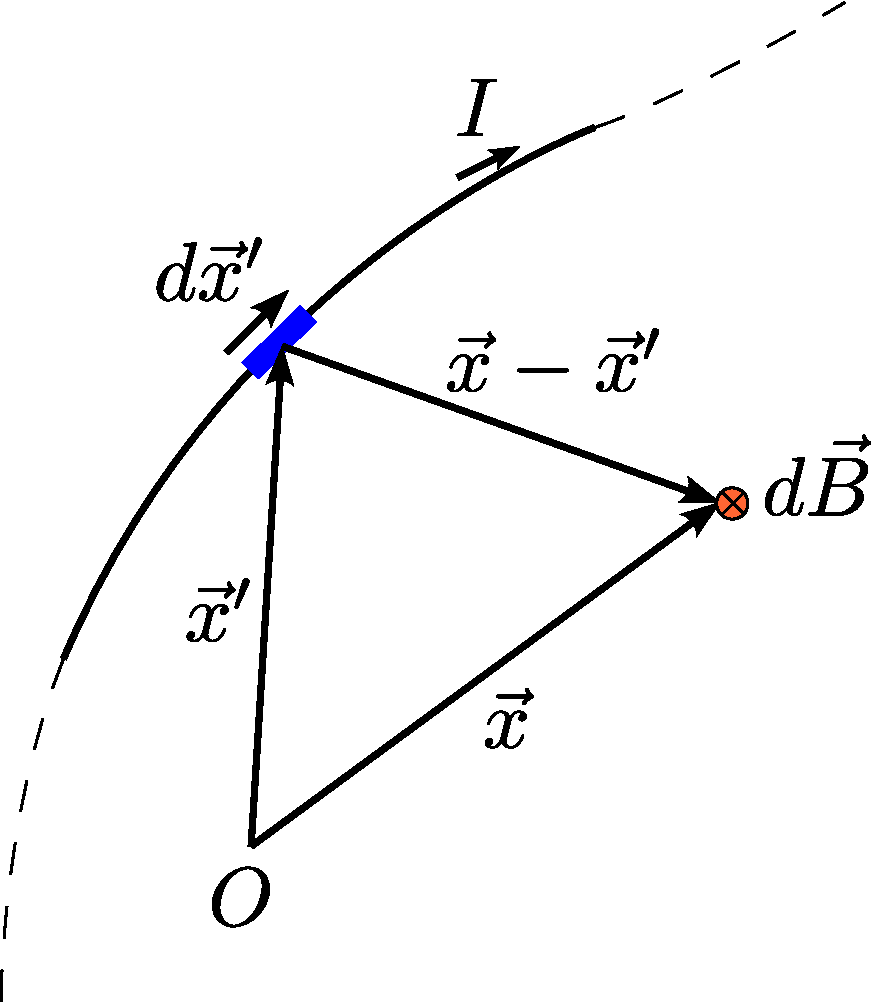
\psfig{file=fig/fig-Biot-Savart-01.pdf,height=6cm,angle=0}}
\label{Esquema para la ley de Biot-Savart.}
\label{fBS1}
\caption{Ley de Biot-Savart.}
\end{figure}
En resumen,
\begin{equation}
dB_i=kI\varepsilon_{ijk}dx'_j\frac{\left(x_k-x'_k\right)}{\left\vert
\vec{x}-\vec{x}'\right\vert^3},
\end{equation}
donde $k$ es una constante, que depende del sistema de unidades usado y que,
en el Sistema Internacional, \textit{se define} como
\begin{equation}
k=\frac{\mu_0}{4\pi}=10^{-7}~\left[  \frac{V\,s}{A\,m}\right],
\end{equation}
y donde $\mu_0$ es llamada la constante de \textbf{permeabilidad magn'etica del vac'io}.

Con esto, escribimos la \textbf{ley de Biot-Savart} como
\begin{equation}
dB_i=\frac{\mu_0}{4\pi}I\,\varepsilon_{ijk}dx'_j\frac{\left(x_k-x'_k\right)}
{\left\vert \vec{x}-\vec{x}'\right\vert ^3}.
\end{equation}
Usando el \textbf{principio de superposici'on} obtenemos una expresi'on para el campo producido por un cable de longitud finita, pero muy delgado:
\begin{equation}
\boxed{B_i(x)=\frac{\mu_0}{4\pi}\int_{\cal C}\varepsilon_{ijk}Idx'_j
\frac{\left(x_k-x'_k\right)}{\left\vert\vec{x}-\vec{x}'\right\vert^3}.}
\label{BS1}
\end{equation}

Podemos generalizar este resultado al caso de una distribuci'on volum'etrica de corriente, descrita por su densidad de corriente. Para esto, consideramos un peque\~no ``tubo de corriente"\, de secci'on transversal $dS$ que sigue las l'ineas de flujo, es decir, tal que el vector normal a la superficie transversal, $\hat{n}$, es paralalo a $\vec{J}$. Entonces, $\vec{J}=J\hat{n}$, $d\vec{x}=d\ell\,\hat{n}$, y adem'as $dV=d\ell\, dS$ (ver figura \ref{fig:tc}), de modo que podemos escribir
\begin{equation}
I\, d\vec{x}=(J dS)(\hat{n}d\ell)=(J\hat{n})(d\ell dS)=\vec{J}\,dV.
\end{equation}
\begin{figure}[!h]
\centerline{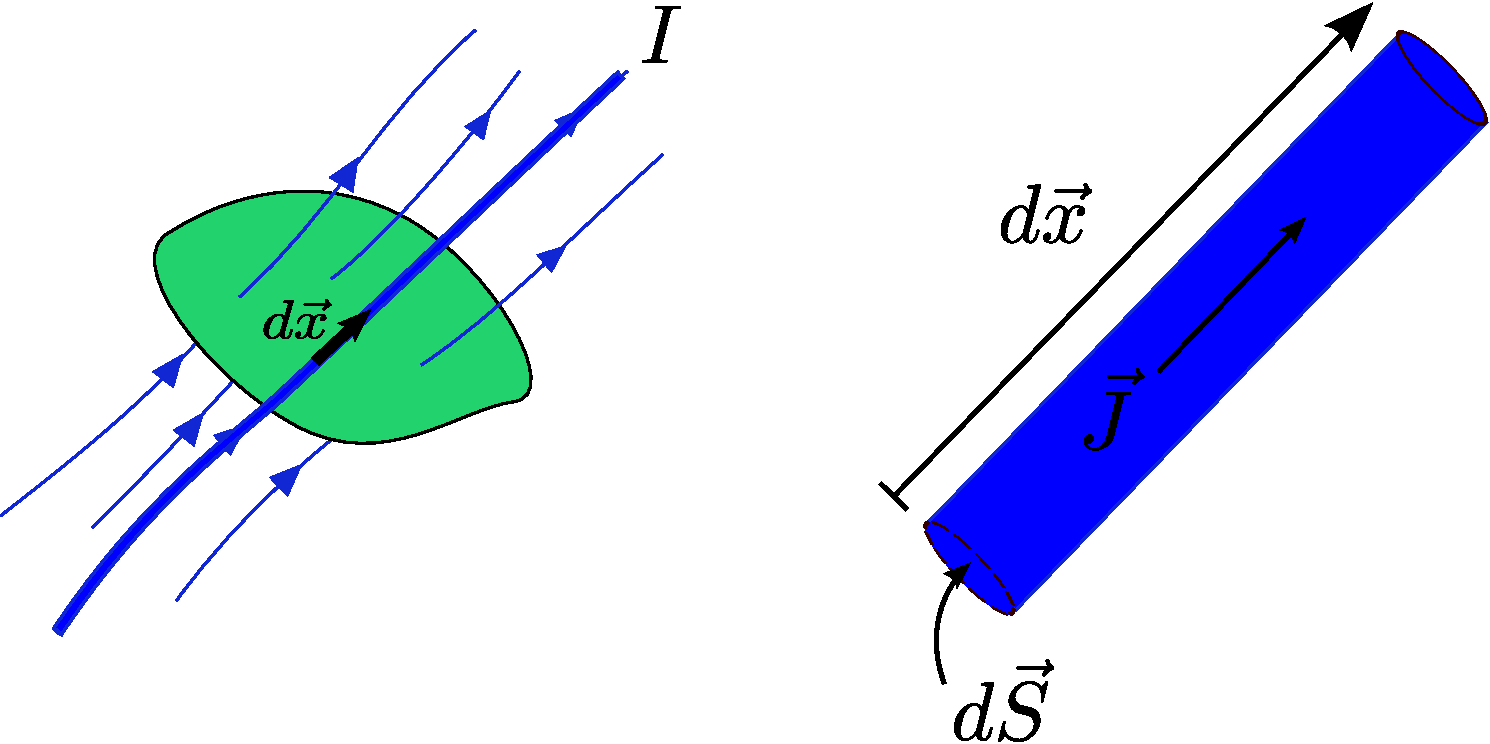
\psfig{file=fig/fig-tubo-de-corriente.pdf,height=4cm,angle=0}}
\caption{Una distribuci'on volum'etrica y los ``tubos de corriente'' asociados.}
\label{fig:tc}
\end{figure}
Con esto podemos encontrar la forma general que usaremos para la ley de Biot-Savart:
\begin{equation}\marginnote{Ley de Biot-Savart}
 \boxed{B_i(x)=\frac{\mu_0}{4\pi}\int_V\varepsilon_{ijk}\,J_j(x')
\frac{\left(x_k-x'_k\right)}{\left\vert\vec{x}-\vec{x}'\right\vert^3}dV'. }
\label{BS2}
\end{equation}
Tambi'en podemos considerar una \textit{distribuci'on superficial de corriente}, es decir una situaci'on donde puede \textit{aproximarse} que la corriente est'a confinada sobre una superficie (de ancho nulo). Para describir esta distribuci'on usamos la \textbf{densidad superficial de corriente}, que denotaremos como $\vec{j}$. Esta densidad superficial es definida tal que
\begin{equation}
\vec{J}\,dV=\vec{j}\,dS,
\end{equation}
donde $dS$ denota el elemento de superficie \textit{sobre} (y no \textit{a trav'es} de) la que fluye la corriente. El campo magn'etico generado por este tipo de distribuciones adopta entonces la forma siguiente:
\begin{equation}
 \boxed{B_i(x)=\frac{\mu_0}{4\pi}\int_S\varepsilon_{ijk}\,j_j(x')
\frac{\left(x_k-x'_k\right)}{\left\vert\vec{x}-\vec{x}'\right\vert^3}dS'. }
\label{BSsup}
\end{equation}
Tal como en el estudio del campo electrost'atico, trabajaremos con la expresi'on volum'etrica \eqref{BS1}, que es m'as general. Si se requiere adaptar las expresiones al caso de corrientes superficiales o lineales pueden entonces usarse las siguientes reglas de conversi'on:
\begin{equation}\label{IdxJdV}
\vec{J}\,dV=\vec{j}\,dS=I\,d\vec{x}.
\end{equation}
Note adem'as que si la corriente es siempre producida por una distribuci'on de cargas movi'endose con velocidad $\vec{v}$ entonces 
\begin{equation}
\vec{J}=\rho\vec{v}, \qquad \vec{j}=\sigma\vec{v}, \qquad I=\lambda v,
\end{equation}
donde $\rho$, $\sigma$ y $\lambda$ son las densidad de carga por unidad de volumen, superficie y longitud, en el caso de distribuciones de corriente volum'etrica, superficial y lineal, respectivamente.

\section{Potencial vectorial}
Consideramos ahora la identidad
\begin{equation}
\frac{x_k-x'_k}{\left\vert
\vec{x}-\vec{x}'\right\vert^3}\equiv -\partial_k\left(
\frac{1}{\left\vert\vec{x}-\vec{x}'\right\vert }\right).
\end{equation}
Reemplaz'andola en (\ref{BS2}) encontramos
\begin{eqnarray}
 B_i(x)&=&-\frac{\mu_0}{4\pi}\int_V\varepsilon_{ijk}\,J_j(x')
\partial_k\left(\frac{1}{\left\vert\vec{x}-\vec{x}'\right\vert }\right)dV'
\label{BS3} \\
&=&-\varepsilon_{ijk}\,\partial_k\left(\frac{\mu_0}{4\pi}\int_VJ_j(x')\frac{1}{
\left\vert\vec{x} -\vec{x}'\right\vert }dV'\right)\\
&=&\varepsilon_{ijk}\,\partial_j\left(\frac{\mu_0}{4\pi}\int_VJ_k(x')\frac{1}{
\left\vert\vec{x} -\vec{x}'\right\vert }dV'\right).
\end{eqnarray}
Por lo tanto, siempre es posible escribir el campo magnetost'atico como el rotor de un campo vectorial,
\begin{equation}\marginnote{Potencial Vectorial}
\boxed{B_i(x)=\varepsilon_{ijk}\,\partial_jA_k(x),}\label{rot-A}
\end{equation}
donde hemos introducido el \textbf{potencial vectorial},
\begin{equation}\marginnote{Pot. Vectorial particular}
\boxed{A_k(x):=\frac{\mu_0}{4\pi}\int_V\frac{J_k(x')}{\left\vert\vec{x}-\vec{x}
'\right\vert }\,dV'.}
\label{defA}
\end{equation}
An'alogamente al caso electrost'atico, el \textit{potencial vectorial no es \'{u}nico}. En el caso magn'etico, sin embargo, la situaci'on es algo menos trivial ya que es posible considerar un nuevo potencial vectorial
\begin{equation}
A'_i:=A_i+\partial_i\Psi(x), \label{gauge01}
\end{equation}
donde $\Psi(x)$ es una \textit{funci'on arbitraria}, y el campo magn'etico
permanecer'a inalterado, ya que $B'_i(x)=\varepsilon_{ijk}\,\partial_jA'_k(x)=B_i(x)$. La transformaci'on (\ref{gauge01}) es llamada una \textbf{transformaci'on de gauge}
del potencial vectorial. Como consecuencia, el potencial vectorial $\vec{A}(x)$
\textit{no es una cantidad medible}, sino m'as bien un campo auxiliar (muy)
'util en muchos c'alculos. En general, a menos que se explicite lo contrario,
cuando hablemos del potencial vectorial magn'etico nos referiremos la elecci'on particular 
dada por (\ref{defA}).


\section{Divergencia del Campo Magn'etico}

Como consecuencia directa de (\ref{rot-A}), vemos que \textit{el campo magnetost'atico
es siempre libre de divergencia}:
\begin{equation}
 \boxed{\vec{\nabla}\cdot\vec{B}=0.} \label{divB}
\end{equation}
Equivalentemente,
\begin{equation}
 \oint_S\vec{B}\cdot d\vec{S}=0,
\end{equation}
es decir, que el \textbf{flujo magn'etico} a trav'es de cualquier superficie cerrada es nulo.

Recordemos que el flujo magn'etico a trav'es de una superficie $S$ es definido
como
\begin{equation}
 \Phi_S:= \int_S\vec{B}\cdot d\vec{S}.
\end{equation}
Usando (\ref{rot-A}) y el teorema de Stokes encontramos que
\begin{equation}\label{PAdx}
 \Phi_S=\oint_{\partial S}\vec{A}\cdot d\vec{x},
\end{equation}
es decir, que el flujo magn'etico a trav'es de una superficie s'olo depende del
valor del potencial vectorial sobre la curva (orientada) $\partial S$ que delimita $S$.
Puede verificarse adem'as que, si bien la expresi'on anterior involucra el
potencial vectorial, \textit{el valor del flujo $\Phi_S$ es independiente de la
elecci'on particular de $\vec{A}$} dentro de la familia de potenciales
vectoriales asociados a un campo $\vec B$ dado. En otras palabras el flujo es
\textbf{invariante} bajo transformaciones de gauge. Note adem'as que, debido a la
relaci'on entre $\Phi_S$ y $\vec{B}$ este 'ultimo vector es tambi'en llamado
\textbf{densidad de flujo magn'etico}. En el sistema internacional de unidades, se define el \textit{Weber}\footnote{En honor a Wilhelm Weber, f'isico alem'an (1804-1891). Ver \url{http://es.wikipedia.org/wiki/Wilhelm_Weber}.} como unidad de flujo magn'etico: $1Wb=1T\cdot 1m^2=1V\cdot 1s$.

\section{Ley de Amp\`ere}

Queremos calcular el rotor de la intensidad de campo magn'etico, es decir, $\varepsilon_{ijk}\partial_jB_k$. Usando (\ref{rot-A})
podemos escribir:
\begin{eqnarray}
 \varepsilon_{ijk}\partial_jB_k&=&\varepsilon_{ijk}\varepsilon_{
klm}\partial_j\partial_lA_m \\
&=&\partial_i(\partial_jA_j) -\partial_j\partial_jA_i. \label{rotB1}
\end{eqnarray}
Para evaluar esta expresi'on usaremos el potencial definido por (\ref{defA})
(el resultado final es independiente de la elecci'on de $\vec{A}$ ya que s'olo
depende de $\vec{B}$). Calculemos primero la divergencia del potencial
vectorial:
\begin{eqnarray}
\partial_iA_i&=&\frac{\mu_0}{4\pi}\int_VJ_i(x')\partial_i\frac{1}{\left\vert\vec
{x} -\vec{x}'\right\vert }\,dV' \\
&=& -\frac{\mu_0}{4\pi}\int_VJ_i(x')\partial'_i\frac{1}{\left\vert\vec{
x } -\vec{x}'\right\vert }\,dV' \\
&=&-\frac{\mu_0}{4\pi}\int_V\left[\partial'_i\left(\frac{J_i(x')}{
\left\vert\vec{x}-\vec{x}'\right\vert}\right)-\frac{
\left(\partial'_iJ_i(x')\right) } { \left\vert\vec{x} -\vec{x}'\right\vert
}\right]\,dV' \\
&=&-\frac{\mu_0}{4\pi}\oint_{\partial V}\frac{J_i(x')}{
\left\vert\vec{x}-\vec{x}'\right\vert}dS'_i+\frac{\mu_0}{4\pi}\int_V\frac{
\left(\partial'_iJ_i(x')\right) } {\left\vert\vec{x}
-\vec{x}'\right\vert}\,dV'  \label{divA} \\
&=&0. \label{divA0}
\end{eqnarray}
El primer t'ermino del lado derecho de (\ref{divA}) se anula cuando cuando $V$
se extiende a todo el espacio, puesto que suponemos que la densidad de corriente
se anula suficientemente r'apido en el infinito (m'as r'apido que $1/r$). Adem'as, el segundo t'ermino es nulo \textit{para corrientes estacionarias}, ver (\ref{divJ0}). Por lo tanto, hemos probado que el potencial (\ref{defA}) tiene divergencia nula en el caso de corrientes
estacionarias confinadas a regiones compactas del espacio.

Debemos ahora calcular el laplaciano (de cada una de las componentes) de
$\vec{A}$. De la definici'on (\ref{defA}) encontramos que
\begin{eqnarray}
 \nabla^2A_i&=&\frac{\mu_0}{4\pi}\int_VJ_i(x')\nabla^2\frac{1}{\left\vert\vec{
x } -\vec{x}'\right\vert }\,dV'\\
&=&\frac{\mu_0}{4\pi}\int_VJ_i(x')\left(-4\pi\delta^{(3)}(\vec{x}-\vec{x}
')\right)\,dV' \\
&=&-\mu_0J_i(x). \label{lapAj}
\end{eqnarray}
Reemplazando (\ref{divA0}) y (\ref{lapAj}) en (\ref{rotB1}) encontramos la
\textbf{ley de Amp\`ere}\footnote{\href{http://es.wikipedia.org/wiki/Andr\%C3\%A9-Marie_Amp\%C3\%A8re}{Andr'e-Marie Amp\`ere} (1775-1836): matem'atico y f'isico franc'es.}:
\begin{equation}
\boxed{\varepsilon_{ijk}\partial_jB_k=\mu_0J_i,}
\end{equation}
o, en notaci'on vectorial,
\begin{equation}\marginnote{Ley Amp\`ere (diferencial)}
 \boxed{\vec\nabla\times\vec{B}=\mu_0\vec{J}.}\label{ley-Ampere}
\end{equation}
La versi'on integral de la ley de Amp\`ere (obtenida integrando
(\ref{ley-Ampere}) en una superficie $S$ con borde $\partial S$, y usando el
teorema de Stokes) es
\begin{equation}\marginnote{Ley Amp\`ere (integral)}
 \boxed{\oint_{\partial S}\vec{B}\cdot d\vec{x}=\mu_0 I_S,}
\end{equation}
donde $I_S=\int_S\vec{J}\cdot d\vec{S}$ es la corriente neta que fluye por $S$.

\subsection{Ejemplo: Campo magn'etico producido por una l'inea infinita de
corriente}
\begin{figure}[!h]
\centerline{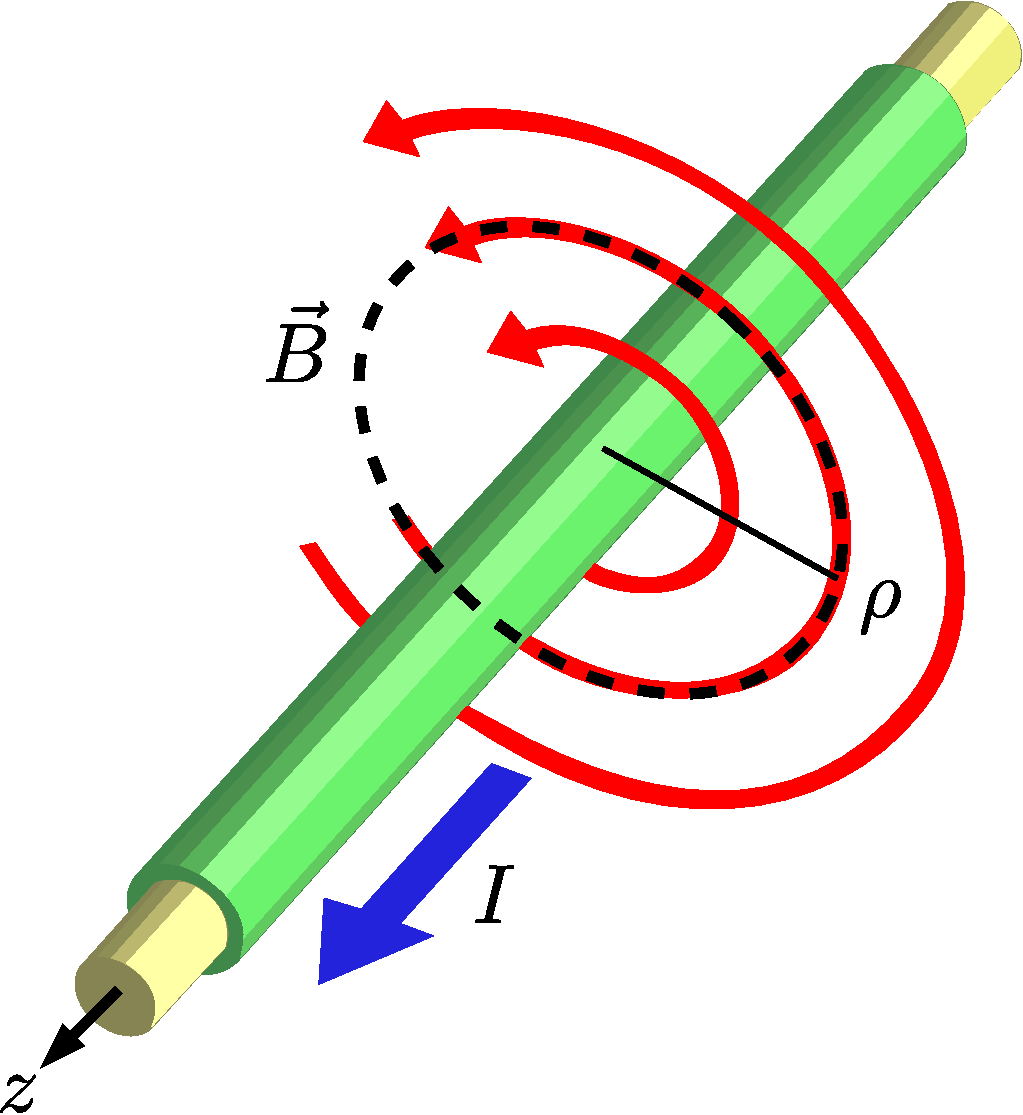
\psfig{file=fig/fig-B-conductor-recto-01.pdf,height=5cm,angle=0}}
\caption{Campo magn'etico producido por un conductor recto. Figura original  \href{http://en.wikipedia.org/wiki/File:Electromagnetism.svg}{aqu\'i}.}
\label{cmcr}
\end{figure}
Aplicando la ley de Amp\`ere a la circunsferencia de radio $\rho$ indicada en la figura
(\ref{cmcr}) encontramos que
\begin{equation}
 \oint_{\cal C}\vec{B}\cdot d\vec{x}=(2\pi \rho)B=\mu_0 I,
\end{equation}
de modo que
\begin{equation}
\vec{B}(\rho)=\frac{\mu_0I}{2\pi}\frac{\hat{\varphi}}{\rho}.
\end{equation}
Un potencial vectorial posible para describir este campo es
\begin{equation}
 \vec{A}_1(\rho)=-\frac{\mu_0I}{2\pi}\ln\frac{\rho}{\rho_0} \hat{z}.
\end{equation}
Sin embargo, otro potencial posible es
\begin{equation}
 \vec{A}_2(z)=\frac{\mu_0I}{2\pi}\frac{z}{\rho} \hat{\rho}.
\end{equation}


\section{Potencial escalar magn'etico}\label{secpem}
En regiones en las que no existen corrientes, $\vec{J}=\vec{0}$, el
rotor del campo magn'etico es nulo, $\vec{\nabla}\times\vec{B}=\vec{0}$. En
este caso es \textit{posible escribir $\vec{B}$ como el gradiente de un campo escalar},
\begin{equation}\marginnote{Potencial Escalar Magn'etico}
 \vec{B}=-\mu_0\vec\nabla\phi^*, \label{Bgradphi}
\end{equation}
donde $\phi^*$ es llamado \textbf{potencial escalar magn'etico}. Ya que adem'as
el campo magn'etico es (siempre) libre de divergencias, tenemos que
\begin{equation}
 \boxed{\nabla^2\phi^*=0,}
\end{equation}
\textit{en regiones sin corrientes}.

Esta propiedad permite en muchos casos aplicar m'etodos similares a aquellos de
la electrost'atica, para determinar el potencial (magn'etico, en este caso)
como soluci'on de la ecuaci'on de Laplace en regiones libres de corrientes,
imponiendo las condiciones de contorno adecuadas para el campo magn'etico.

\section{Expansi'on multipolar magn'etica}\label{sec:emm}
\begin{figure}[!h]
\centerline{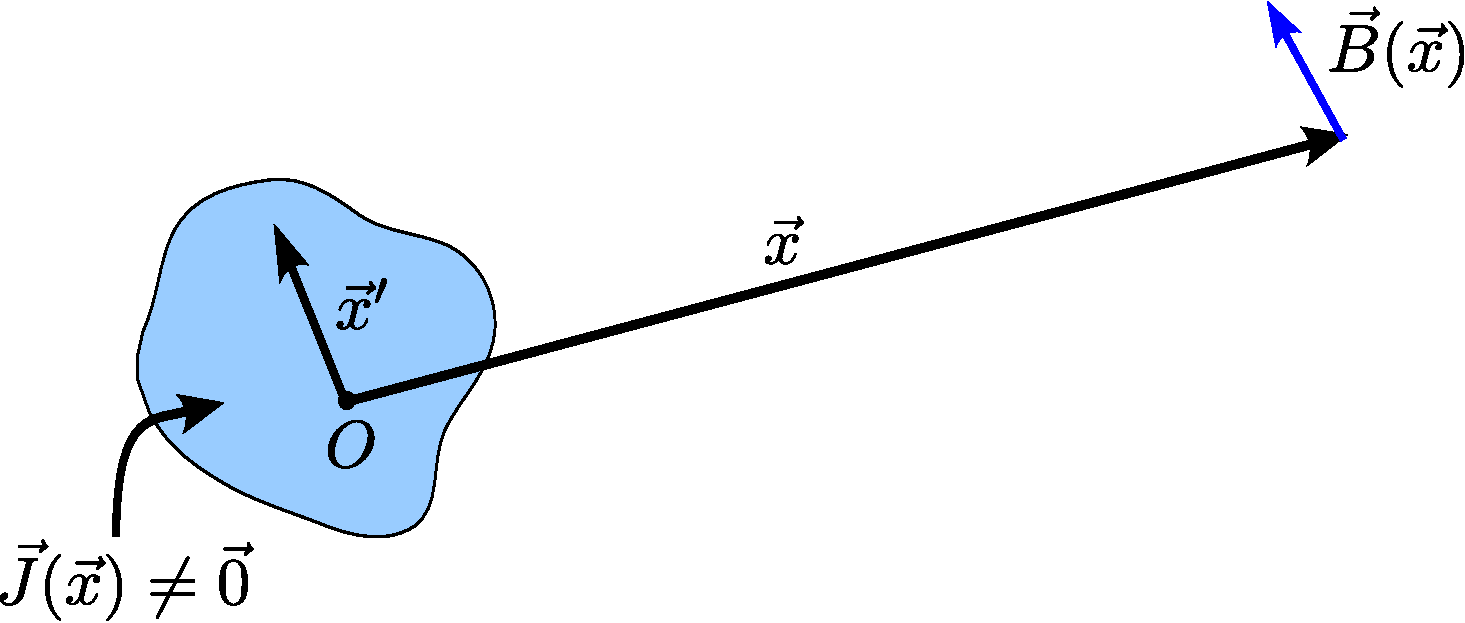
\psfig{file=fig/fig-expansion-multipolar-magnetica-01.pdf,height=4cm,
angle=0 } }
\caption{Esquema de la expansi'on multipolar magn'etica.}
\label{MM1}
\end{figure}
An'alogamente al caso electrost'atico, deseamos calcular el campo
magn'etico $\vec{B}$ lejos de una distribuci'on  de corrientes, descritas por una densidad de corriente $\vec{J}$, localizada en una regi'on peque\~na comparada con la distancia a la cual se calcular'a el campo.

Situando el origen en un punto representativo de la distribuci'on de
corrientes, tendremos que para distancias grandes comparadas con el
tama\~no de la distribuci'on se satisface $\left\vert\vec{x}\right\vert \gg\left\vert
\vec{x}'\right\vert $,\ ver figura \ref{MM1}. Con esto, podemos usar la
expansi'on (\ref{exp1or}) y reescribir la expresi'on (\ref{defA}) como una
expansi'on multipolar magn'etica:
\begin{equation}
 A_i(x)=\frac{\mu_0}{4\pi}\sum_{n=0}^\infty \frac{(-1)^n}{n!}M_{i_1\cdots
i_ni}\partial_{i_1}\cdots \partial_{i_n}\frac{1}{r},
\end{equation}
donde hemos definidos los \textbf{momentos multipolares magn'eticos} como
\begin{equation}
\boxed{ M_{i_1\cdots i_ni}:=\int_V x_{i_1}\cdots x_{i_n}\,J_i(x)\,dV.}
\end{equation}
Note que, debido al caracter vectorial de la densidad de corriente, el momento
multipolar magn'etico de orden $n$ es un tensor de orden $n+1$.

En la pr'actica es com'un usar s'olo los primeros t'erminos de la expansi'on
multipolar magn'etica. Adem'as, el t'ermino monopolar magn'etico es siempre
identicamente nulo \textit{para corrientes estacionarias}, ya que
\begin{equation}
 M_i=\int_V J_i(x)\,dV=0. \label{mmm0}
\end{equation}
Para probar esto, considere la siguiente integral $\oint_{\partial V}x_i
J_j\,dS_j$. Usando el teorema de Gauss podemos escribir
\begin{equation}
 \oint_{\partial V}x_i
J_j\,dS_j=\int_V\partial_j(x_iJ_j)\,dV=\int_V\left[
(\partial_jx_i)J_j+x_i(\partial_jJ_j)\right]\,dV=\int_V\left[
\delta_{ij}J_j+0\right]\,dV
\end{equation}
En la 'ultima igualdad usamos el hecho que para corrientes estacionarias la
divergencia del vector densidad de corriente es nula, ver \eqref{divJ0}. Con esto, encontramos la
identidad
\begin{equation}
  \int_VJ_i\,dV\equiv \oint_{\partial V}x_iJ_j\,dS_j.
\end{equation}
Esta identidad es v'alida para cualquier volumen $V$. Entonces para probar lo
requerido basta considerar un volumen que \textit{contiene totalmente}
la distribuci'on de corrientes, de modo que $\vec{J}=\vec{0}$ en la superficie
$\partial V$.

Este resultado general (para corrientes estacionarias) tiene como consecuencia
que \textit{la expansi'on multipolar magn'etica comienza con el t'ermino
dipolar} ($n=1$).

El momento multipolar de orden 1 es dado por
\begin{equation}
 M_{ij}=\int_V x_i\,J_j(x)\,dV.
\end{equation}

Es posible probar que este tensor es \textit{antisim'etrico},
$M_{ij}=-M_{ji}$, \textit{para distribuciones de corrientes estacionarias}. Para esto,
basta analizar la integral $\oint_{\partial V}x_i x_j J_k\,dS_k$ de forma
an'aloga a lo discutido anteriormente, es decir, aplicando el teorema de Gauss y la
condici'on de divergencia nula de la densidad de corriente. Ya que $M_{ij}$ es
antisim'etrico, \textit{la informaci'on que este tensor contiene puede ser
equivalentemente descrita en t'erminos de un (pseudo-) vector} $\vec{\mu}$,
llamado \textbf{momento (dipolar) magn'etico}, y definido por
\begin{equation}
 \mu_i:=\frac{1}{2}\varepsilon_{ijk}M_{jk}, \qquad
M_{ij}=\varepsilon_{ijk}\mu_k, \label{vmdm}
\end{equation}
es decir,
\begin{equation}
 \boxed{\mu_i=\frac{1}{2}\varepsilon_{ijk}\int_V x_j J_k(x)\, dV,}
\end{equation}
o, en notaci'on vectorial, 
\begin{equation}
 \boxed{\vec{\mu}=\frac{1}{2}\int_V \vec{x}\times\vec{J}(x)\,dV,}
\end{equation}
Con esto, el t'ermino dipolar de la expansi'on multipolar magn'etica para el
potencial vectorial \eqref{defA} es
\begin{eqnarray}
 A_i^{(1)}(x)&=&-\frac{\mu_0}{4\pi}M_{ji}\partial_j\frac{1}{r} \\
&=&-\frac{\mu_0}{4\pi}\left(\varepsilon_{jil}\mu_l\right)\left(-\frac{x_j}{
r^3}\right) \\
&=&\frac{\mu_0}{4\pi}\varepsilon_{ijk}\frac{\mu_jx_k}{r^3},
\end{eqnarray}
es decir,
\begin{equation}
 \boxed{\vec{A}^{(1)}(x)=\frac{\mu_0}{4\pi}\frac{\vec{\mu}\times\vec{x}}{r^3}.}
\label{Adip}
\end{equation}
M'as importante que el potencial, que sabemos no es 'unico, es el campo
magn'etico. La contribuci'on dipolar al campo generado por una distribuci'on
compacta de corriente es entonces dado por
\begin{eqnarray}
B_i^{(1)}(x)&=&\varepsilon_{ijk}\partial_jA_k^{(1)}(x)\\
&=&\varepsilon_{ijk}\partial_j\left(\frac{\mu_0}{4\pi}\varepsilon_{klm}\frac{
\mu_lx_m}{r^3}\right) \\
&=&\frac{\mu_0}{4\pi}\varepsilon_{ijk}\varepsilon_{klm}\mu_l\partial_j\left(
\frac{x_m}{r^3}\right) \\
&=&\frac{\mu_0}{4\pi}\left(\delta_{il}\delta_{jm}-\delta_{jl}\delta_{im}\right)
\mu_l\left(\frac{\delta_{jm}}{r^3}-3\frac{x_mx_j}{r^5}\right) \\
&=&\frac{\mu_0}{4\pi}\left[3\frac{x_i(x_j\mu_j)}{r^5}-\frac{\mu_i}{r^3}
\right] ,
\end{eqnarray}
o, en notaci'on vectorial
\begin{equation}
\boxed{\vec{B}^{(1)}=\frac{\mu_0}{4\pi}\left[\frac{3\hat{r}(\vec{\mu}
\cdot\hat{r}) -\vec{\mu}}{r^3}\right] , \qquad \hat{r}:=\frac{\vec{x}}{r}.}
\end{equation}
\begin{figure}[!h]
\centerline{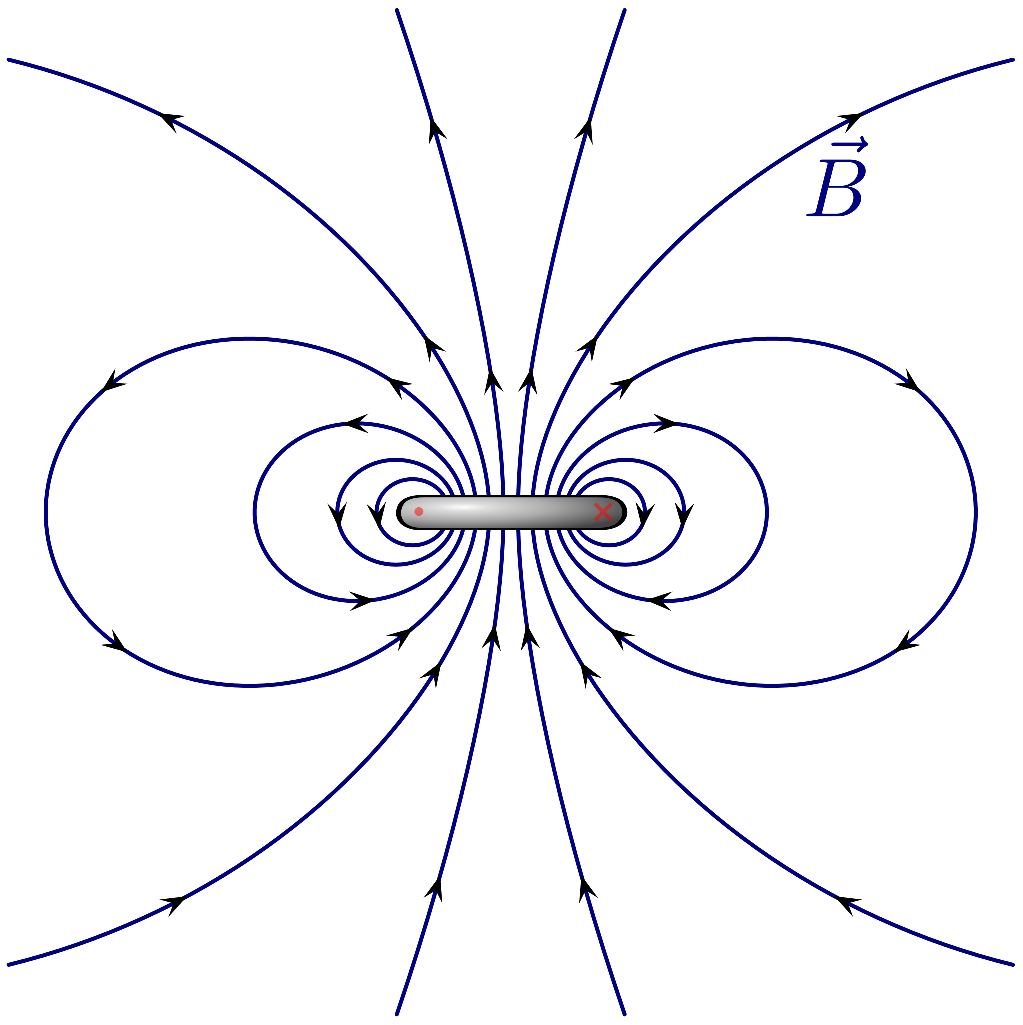
\psfig{file=fig/fig-campo-magnetico-espira.pdf,height=5cm,angle=0}\hspace{2cm}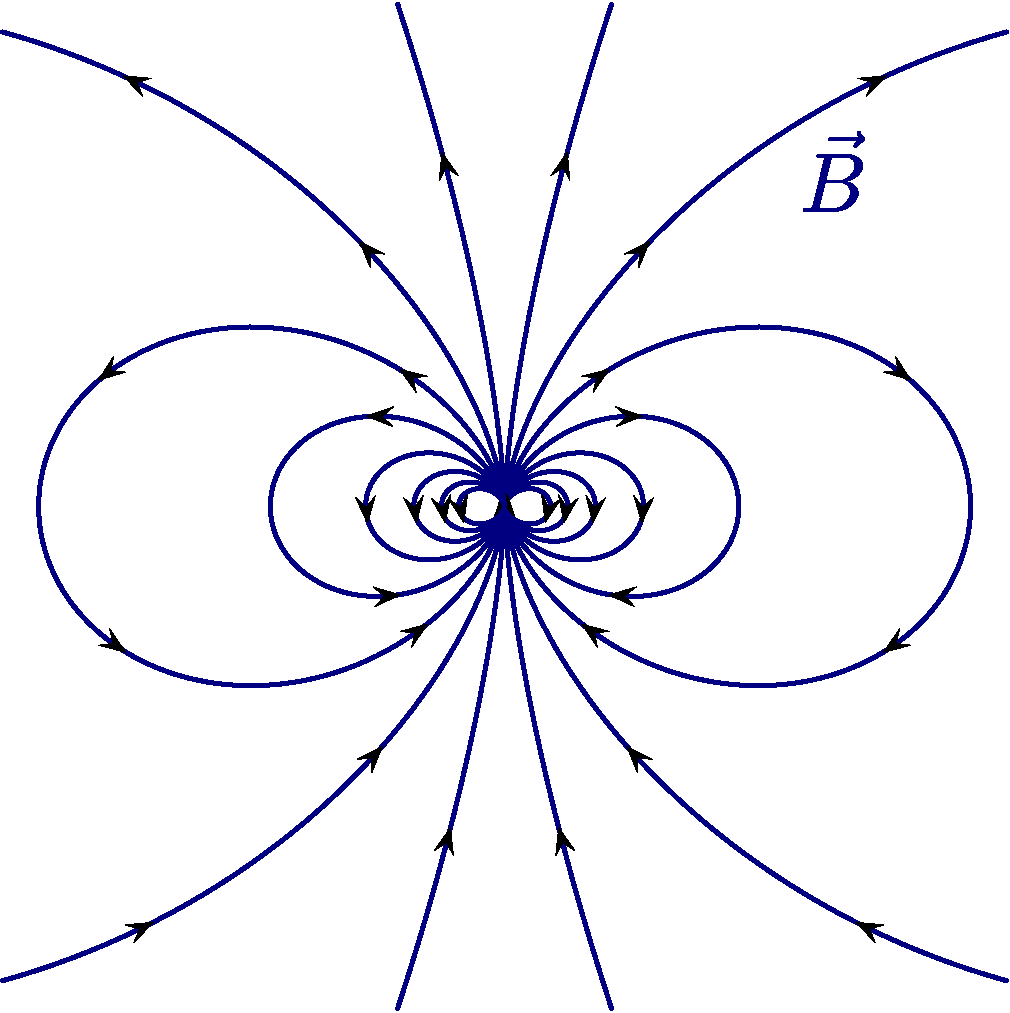
\psfig{file=fig/fig-campo-dipolo-magnetico.pdf,height=5cm,angle=0}}
\caption{a) Campo magn'etico de una espira, b) campo magn'etico de un dipolo ideal. Adaptadas a partir de \href{http://commons.wikimedia.org/wiki/File:VFPt_dipole_point.svg}{esta} y \href{http://commons.wikimedia.org/wiki/File:VFPt_dipole_magnetic3.svg}{esta} figuras originales.}
\label{fig:dipmag}
\end{figure}

\subsection{Momento dipolar de una espira plana}
\begin{figure}[!h]
\centerline{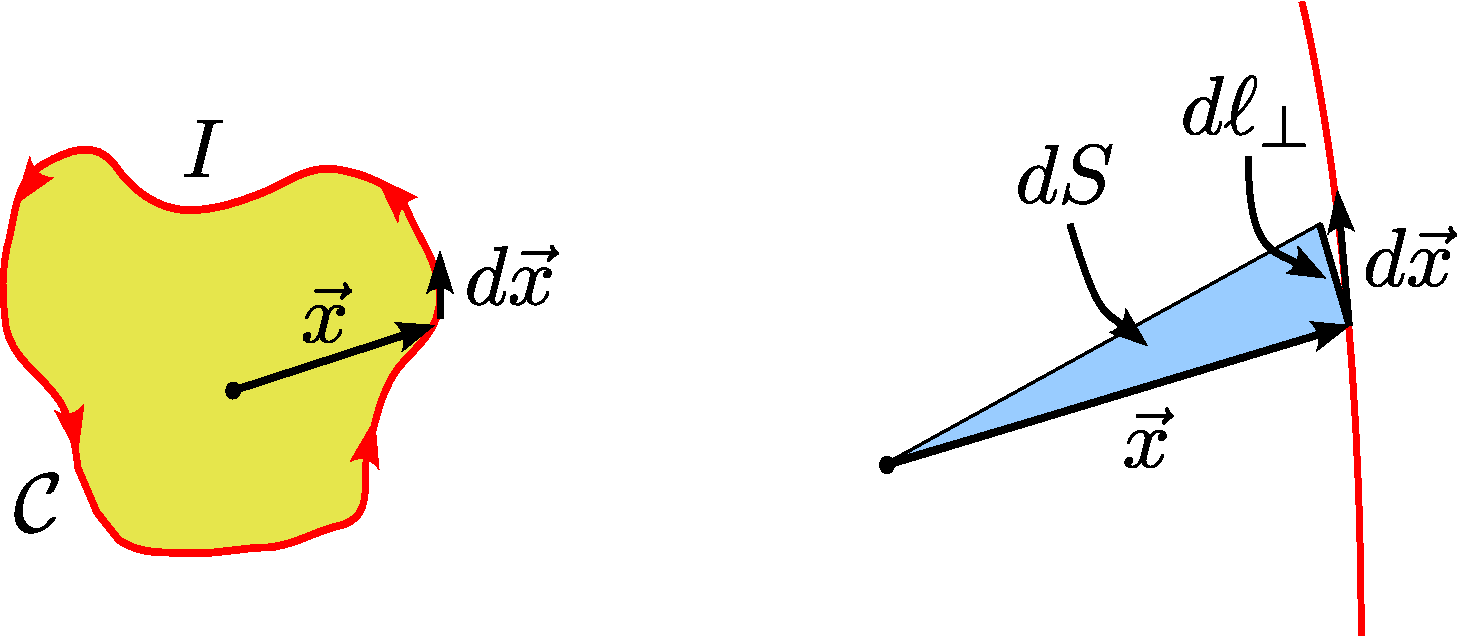
\psfig{file=fig/fig-espira-plana-01.pdf,height=4cm,angle=0}}
\caption{Espira plana y elemento de 'area.}
\label{fep01}
\end{figure}
En el caso de que la distribuci'on de corriente se concentre en conductores que
describen una curva $\cal C$ (sobre un plano) y transportan corriente $I$, el momento magn'etico
es dado por
\begin{equation}\label{muintC}
 \vec{\mu}=\frac{I}{2}\oint_{\cal C} \vec{x}\times d\vec{x}.
\end{equation}
En el caso de un \textit{espira plana}, pero de forma arbitraria, tenemos que
(situando el origen en un punto del mismo plano), $\vec{x}\times
d\vec{x}/2=rd\ell_\bot\hat{n}/2=dS\,\hat{n}$, donde $\hat{n}$ es el
vector normal a la espira cuya con direcci'on dada por la regla de la mano
derecha aplicada a la curva orientada de acuerdo al sentido de circulaci'on de
la corriente\footnote{Equivalentemente, puede obtener este resultado a partir de \eqref{muintC} usando el teorema de Stokes.}. Con esto obtenemos que el momento magn'etico de una espira plana
de 'area $A$ es siempre de la forma
\begin{equation}\marginnote{Momento magn'etico espira plana}
 \boxed{\vec{\mu}=IA\,\hat{n}.}
\end{equation}

\subsection{Relaci'on entre momento magn'etico y momento angular}
En algunos sistemas se tiene que la densidad de carga el'ectrica (en cada
punto) es proporcional a la densidad de masa, de modo que
\begin{equation}
 \rho(x)=\frac{Q}{M} \rho_{\rm m}(x).
\end{equation}
donde $Q$ es la carga total y $M$ la masa total del sistema. Esto ocurre, en
general, en sistemas constituidos por \textit{un s'olo tipo de part'iculas},
masivas y cargadas. En este caso, si cada elemento del sistema se mueve
con velocidad $\vec{v}(x)$, entonces
\begin{equation}
\vec{J}=\rho(x)\vec{v}(x)=\frac{Q}{M} \rho_{\rm m}(x)\vec{v}(x)
\end{equation}
y entonces el momento magn'etico puede escribirse como
\begin{equation}
 \vec{\mu}=\frac{1}{2}\int_V \vec{x}\times\vec{J}\,dV=\frac{Q}{2M}\int_V
\vec{x}\times\rho_{\rm m}(x)\vec{v}(x)\,dV=\frac{Q}{2M}\int_V
\vec{x}\times d\vec{p},
\end{equation}
donde $d\vec{p}:=\rho_{\rm m}(x)\vec{v}(x)\,dV$ denota el \textbf{momentum lineal} de la masa en el elemento de volumen $dV$. De esta forma $d\vec{L}:=\vec{x}\times d\vec{p}$ es el \textbf{momento angular} del peque\~no elemento de masa (respecto al origen elegido) y, finalmente,
\begin{equation}
 \boxed{\vec{\mu}=\frac{Q}{2M}\vec{L}.}
\end{equation}

\section{Fuerza y torque sobre una distribuci'on compacta de corriente}
Consideramos ahora el caso en que una peque\~na distribuci'on de corriente
se ubica en una regi'on donde existe un campo magn'etico \textit{externo}
$\vec{B}(x)$.

La fuerza total que la distribuci'on de corrientes experimenta, debido al campo
externo (es decir, sin tomar en cuenta la autointeracci'on de la distribuci'on),
es dada por (\ref{fm1}). Para expresar esta fuerza en t'erminos de los momentos multipolares magn'eticos de la distribuci'on, situamos nuevamente el
origen de coordenadas en un punto representativo de la distribuci'on y expandimos la
intensidad de campo magn'etico en puntos dentro de 'esta en una serie
de potencias de las componentes del $\vec{x}'$:
\begin{align}
 B_i(\vec{x}+\vec{x}') &= \sum_{n=0}^\infty \frac{1}{n!}x'_{i_1}\cdots x'_{i_n}(\partial_{i_1}\cdots\partial_{i_n}B_i)(x) \label{expB} \\
 &= B_i(x)+x'_j(\partial_jB_i)(x) +
\frac{1}{2}x'_jx'_k(\partial_j\partial_kB_i)(x)+\cdots .
\end{align}
Reemplazando esto en (\ref{fm1}), y tomando en cuenta que la integral sobre la regi'on con corrientes es sobre la variable $\vec{x}'$, encontramos
\begin{align}
F^{\rm m}_i &=  \varepsilon_{ijk}\sum_{n=0}^\infty\frac{1}{n!}M_{i_1\cdots i_nj}(\partial_{i_1}\cdots\partial_{i_n}B_k)(x)\\
&= \varepsilon_{ijk}\left[M_jB_k(x)+M_{lj}(\partial_lB_k)(x)+\frac{1}{2}M_{lnj}(\partial_l\partial_nB_k)(x) +\cdots\right].
\end{align}
Usando (\ref{mmm0}) y (\ref{vmdm}) obtenemos
\begin{eqnarray}
F^{\rm m}_i
&=&\varepsilon_{ijk}\varepsilon_{ljm}\,\mu_m (\partial_lB_k)(x)+\cdots \\
&=& \mu_j(\partial_iB_j)(x)-\mu_i(\partial_jB_j)(x)+\cdots .
\end{eqnarray}
Finalmente, usando la ecuaci'on de campo (\ref{divB}) llegamos a
\begin{equation}
 \boxed{F^{\rm m}_i=\mu_j(\partial_iB_j)(x)+\cdots .}
\end{equation}
En otras palabras, la primera contribuci'on en la expansi'on multipolar a la
fuerza neta sobre una distribuci'on arbitraria es dada por el t'ermino dipolar,
con
\begin{equation}
 \boxed{F_i^{\rm m,(1)}=-\partial_i U_{\rm m}, }
\end{equation}
donde hemos introducido la \textbf{energ'ia de interacci'on entre un dipolo magn'etico
y un campo externo}
\begin{equation}
 \boxed{U_{\rm m}(x)=-\vec{\mu}\cdot\vec{B}(x).} \label{Umagdip}
\end{equation}

Similarmente, el torque neto sobre la espira (con respecto al punto de referencia $O$)  puede calcularse a partir de
\begin{equation}
 \tau_i=\varepsilon_{ijk}\int_V x'_j f^{\rm m}_k(x') dV',
\end{equation}
donde $f^{\rm m}_k$ son las componentes de la densidad de fuerza magn'etica,
definida en (\ref{dfm}). Por lo tanto, usando nuevamente la expansi'on
(\ref{expB}) podemos escribir,
\begin{eqnarray}
  \tau_i&=&\varepsilon_{ijk}\varepsilon_{kln}\int_V x'_j J_l(x')B_n(x')\, dV' \\
&=&\varepsilon_{ijk}\varepsilon_{kln}\int_V x'_j
J_l(x')\left[B_n(x)+x'_p(\partial_pB_n)_(x) +\cdots\right] dV \\
&=&\varepsilon_{ijk}\varepsilon_{kln}\left[M_{jl}B_n(x)+M_{jpl}(\partial_pB_n)(x)
+\cdots\right] \\
&=&\varepsilon_{ijk}\varepsilon_{kln}\varepsilon_{jlp}\,\mu_pB_n(x)+\cdots\\
&=&\varepsilon_{ijk}\,\mu_jB_k(x)+\cdots 
\end{eqnarray}
o, en notaci'on vectorial
\begin{equation}
 \boxed{\vec{\tau}=\vec{\mu}\times\vec{B}+\cdots .} \label{torqueB}
\end{equation}
Puede verificarse usando (\ref{Umagdip}) y (\ref{torqueB}) que un dipolo
magn'etico (o, en primera aproximaci'on, toda distribuci'on compacta de
corriente) situado en un campo (homog'eneo) externo experimentar'a un torque
que tender'a a \textit{alinear} el momento magn'etico de la distribuci'on con el
del campo externo. La posici'on de equilibrio corresponde al caso en que
$\vec{\mu}$ es paralelo a $\vec{B}$, que es adem'as un equilibrio estable ya
que la energ'ia de interacci'on es m'inima. M'as generalmente, el momento
magn'etico puede realizar un \textbf{movimiento de precesi'on} en torno al campo
magn'etico.

%\subsection{Ejemplo: Precesi'on de Larmor}

\section{Campos magn'eticos en la materia}
An'alogamente al caso electrost'atico, en el que un medio se polariza en
presencia de un campo externo, 'este puede adem'as \textit{magnetizarse}. Esto
significa que en cada peque\~no elemento de volumen (macrosc'opico) puede existir un momento magn'etico no nulo. Este momento magn'etico puede ser producto de
los peque\~nos ``loops''\, de corrientes inducidas por el campo aplicado sobre los
electrones at'omicos. Este tipo de dipolos se inducen en \textit{direcci'on contraria}
al campo aplicado, por lo que tienden a \textit{reducir} el valor de la inducci'on
magn'etica al interior del material. Los materiales \textbf{diamagn'eticos} son aquellos en que este tipo de magnetizaci'on es dominante. El hecho que las
part'iculas subat'omicas, y en particular los electrones, posean \textit{momentos
magn'eticos intr'insecos} (permanentes), hace posible que un material presente
magnetizaci'on no nula, de origen distinto a la generada por las corrientes
inducidas. En general, un campo magn'etico aplicado tender'a a alinear, en
mayor o menor medida, los momentos magn'eticos permanentes del material con el campo aplicado, pudiendo compensar y revertir la magnetizaci'on debida a las corrientes
inducidas. Los materiales paramagn'eticos presentan momentos magn'eticos
netos en la misma direcci'on del campo aplicado. En los ferromagnetos, por
otro lado, la alineaci'on de los momentos magn'eticos permanentes es tal que el
momento magn'etico total es no nulo en ausencia de un campo aplicado, y puede asumir valores varios ordenes de magnitud mayor que el caso de los paramagnetos.

\subsection{Magnetizaci'on}
En resumen, consideraremos que en el interior de un medio, existen momentos
magn'eticos distribuidos en su interior. Modelaremos esta distribuci'on
definiendo el \textbf{(pseudo-)vector de magnetizaci'on} como la densidad de momento
magn'etico, es decir, como el momento magn'etico por unidad de volumen en una
peque\~na regi'on ($\Delta V\to 0$, desde el punto de vista macrosc'opico) del
material:
\begin{equation}\marginnote{Definici'on Magnetizaci'on}
\vec{M}(x):= \lim_{\Delta V\to 0} \frac{\Delta \vec{\mu}}{\Delta V}.
\end{equation}
Como consecuencia, la magnetizaci'on tiene unidades de corriente por unidad de
longitud: $[\vec{M}]={[\vec{\mu}]}/{L^3}={IL^2}/{L^3}={I}/{L}$.
Con esta definici'on, tenemos que el momento magn'etico $d\vec{\mu}(x)$
contenido en un elemento de volumen (macrosc'opico) $dV$ centrado en un punto con  posici'on
$\vec{x}$ es
\begin{equation}
d\vec{\mu}(x)=\vec{M}(x)\,dV.
\end{equation}
Entonces, a partir de (\ref{Adip}) podemos calcular al campo (potencial
vectorial) producido por la distribuci'on de momentos dipolares como la
superposici'on del campo correspondiente al momento dipolar magn'etico contenido en cada
elemento de volumen:
\begin{eqnarray}
 A_i^{\rm M}(x)&=&\frac{\mu_0}{4\pi}\varepsilon_{ijk}\int_V
\frac{d\mu_j(x')(x_k-x'_k)}{ \left\vert\vec{x} -\vec{x}'\right\vert^3} \\
&=& \frac{\mu_0}{4\pi}\varepsilon_{ijk}\int_V \frac{M_j(x')(x_k-x'_k)}{
\left\vert\vec{x} -\vec{x}'\right\vert^3}dV'.
\end{eqnarray}
Usando la identidad (\ref{id01}) podemos escribir este potencial vectorial
producido por la magnetizaci'on del material como:
\begin{eqnarray}
  A_i^{\rm M}(x)&=& \frac{\mu_0}{4\pi}\varepsilon_{ijk}\int_V
M_j(x')\partial'_k\frac{1}{\left\vert\vec{x} -\vec{x}'\right\vert}dV'
\label{AM1}\\
&=& \frac{\mu_0}{4\pi}\varepsilon_{ijk}\int_V\left[\partial'_k\left(
\frac{M_j(x')}{\left\vert\vec{x}
-\vec{x}'\right\vert}\right)-\frac{(\partial'_kM_j(x'))}{\left\vert\vec{x}
-\vec{x}'\right\vert}\right]dV' \\
&=&\frac{\mu_0}{4\pi}\oint_{\partial
V}\frac{\varepsilon_{ijk}M_j(x')}{\left\vert\vec{x}
-\vec{x}'\right\vert}dS'_k+\frac{\mu_0}{4\pi}\int_V\frac{(\varepsilon_{ijk}
\partial'_jM_k(x'))}{ \left\vert\vec{x}-\vec{x}'\right\vert}dV' \\
&=&\frac{\mu_0}{4\pi}\oint_{\partial
V}\frac{(\varepsilon_{ijk}M_j(x')\hat{n}_k)}{\left\vert\vec{x}
-\vec{x}'\right\vert}dS'+\frac{\mu_0}{4\pi}\int_V\frac{(\varepsilon_{ijk}
\partial'_jM_k(x'))}{ \left\vert\vec{x}-\vec{x}'\right\vert}dV'  \\
&=&\frac{\mu_0}{4\pi}\oint_{\partial
V}\frac{j^{\rm M,S}_i(x')}{\left\vert\vec{x}
-\vec{x}'\right\vert}dS'+\frac{\mu_0}{4\pi}\int_V\frac{J^{\rm M}_i(x')}{
\left\vert\vec{x}-\vec{x}'\right\vert}dV'.
\end{eqnarray}
En resumen
\begin{equation}
 \boxed{\vec{A}^{\rm M}(x)=\frac{\mu_0}{4\pi}\int_V\frac{\vec{J}^{\rm M}(x')}{
\left\vert\vec{x}-\vec{x}'\right\vert}dV'+\frac{\mu_0}{4\pi}\oint_{\partial
V}\frac{\vec{j}^{\rm M}(x')}{\left\vert\vec{x}-\vec{x}'\right\vert}dS',}
\label{AM01}
\end{equation}
donde hemos definido la \textbf{densidad de corriente de magnetizaci'on}
$\vec{J}^{\rm M}$ y la \textbf{densidad de corriente superficial de
magnetizaci'on} $\vec{j}^{\rm M}$ por
\begin{equation}\marginnote{corrientes de magnetizaci'on}
\boxed{\vec{J}^{\rm M}(x):=\vec\nabla\times\vec{M}(x), \qquad \vec{j}^{\rm
M}(x):=\vec{M}(x)\times\hat{n}(x).}
\end{equation}
Estas definiciones de densidades de corriente, que pueden ser reales o
ficticias dependiendo del origen de la magnetizaci'on $\vec{M}$, son de utilidad
puesto que, de acuerdo a (\ref{AM01}), el campo producido por la magnetizaci'on
es \textit{equivalente} al campo producido (a trav'es de la ley de Biot-Savart)
por las corrientes descritas por $\vec{J}^{\rm M}$ en el interior del material y
por $\vec{j}^{\rm M}$ en su superficie.

\begin{figure}[!h]
\centerline{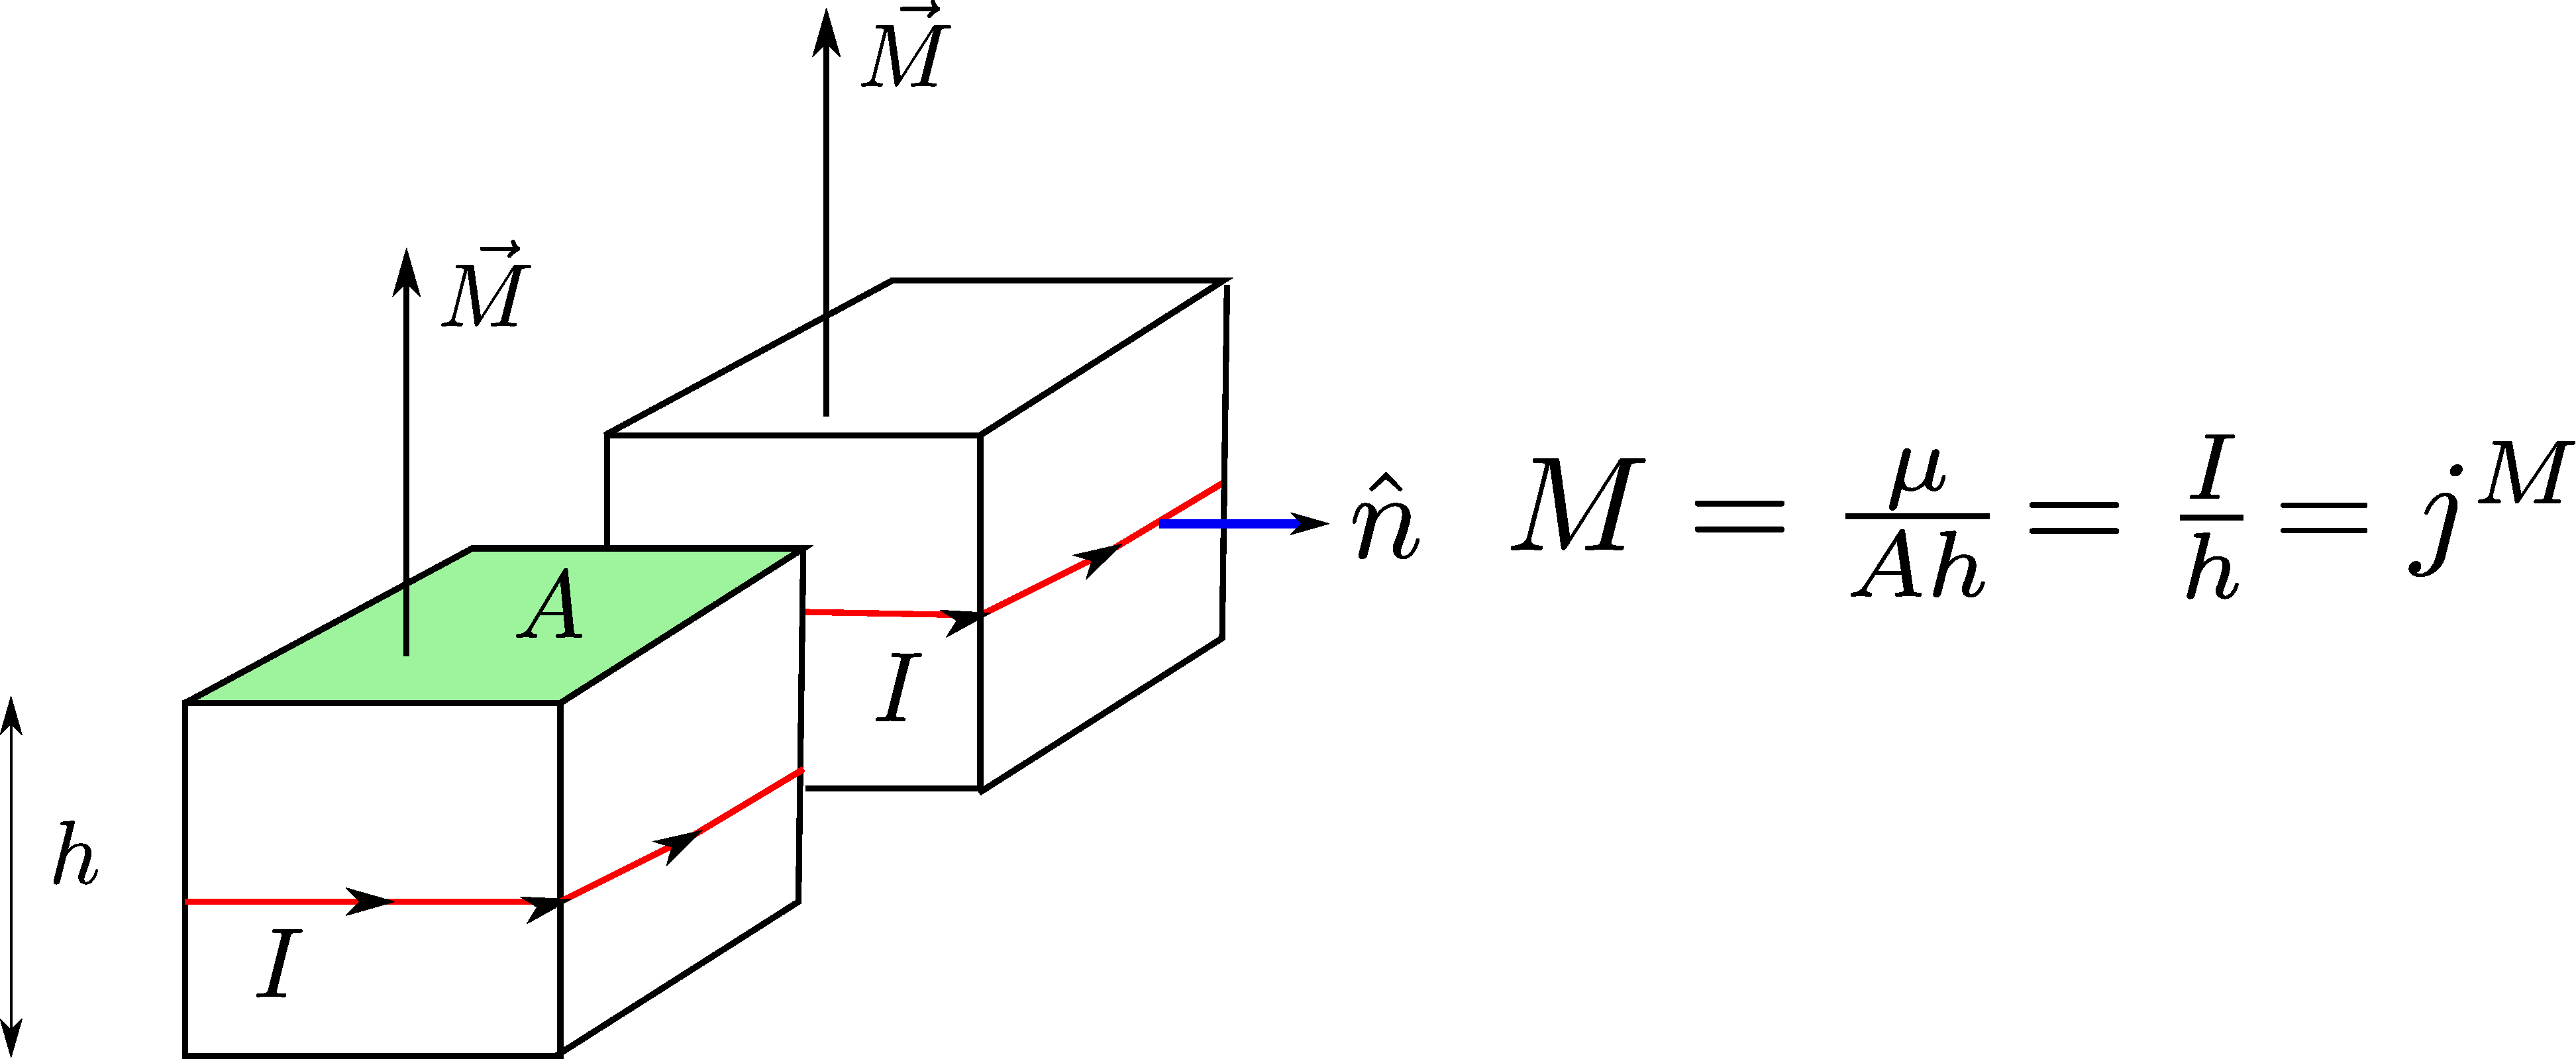
\psfig{file=fig/fig-corriente-magnetizacion-superficie.pdf,height=3cm,angle=0}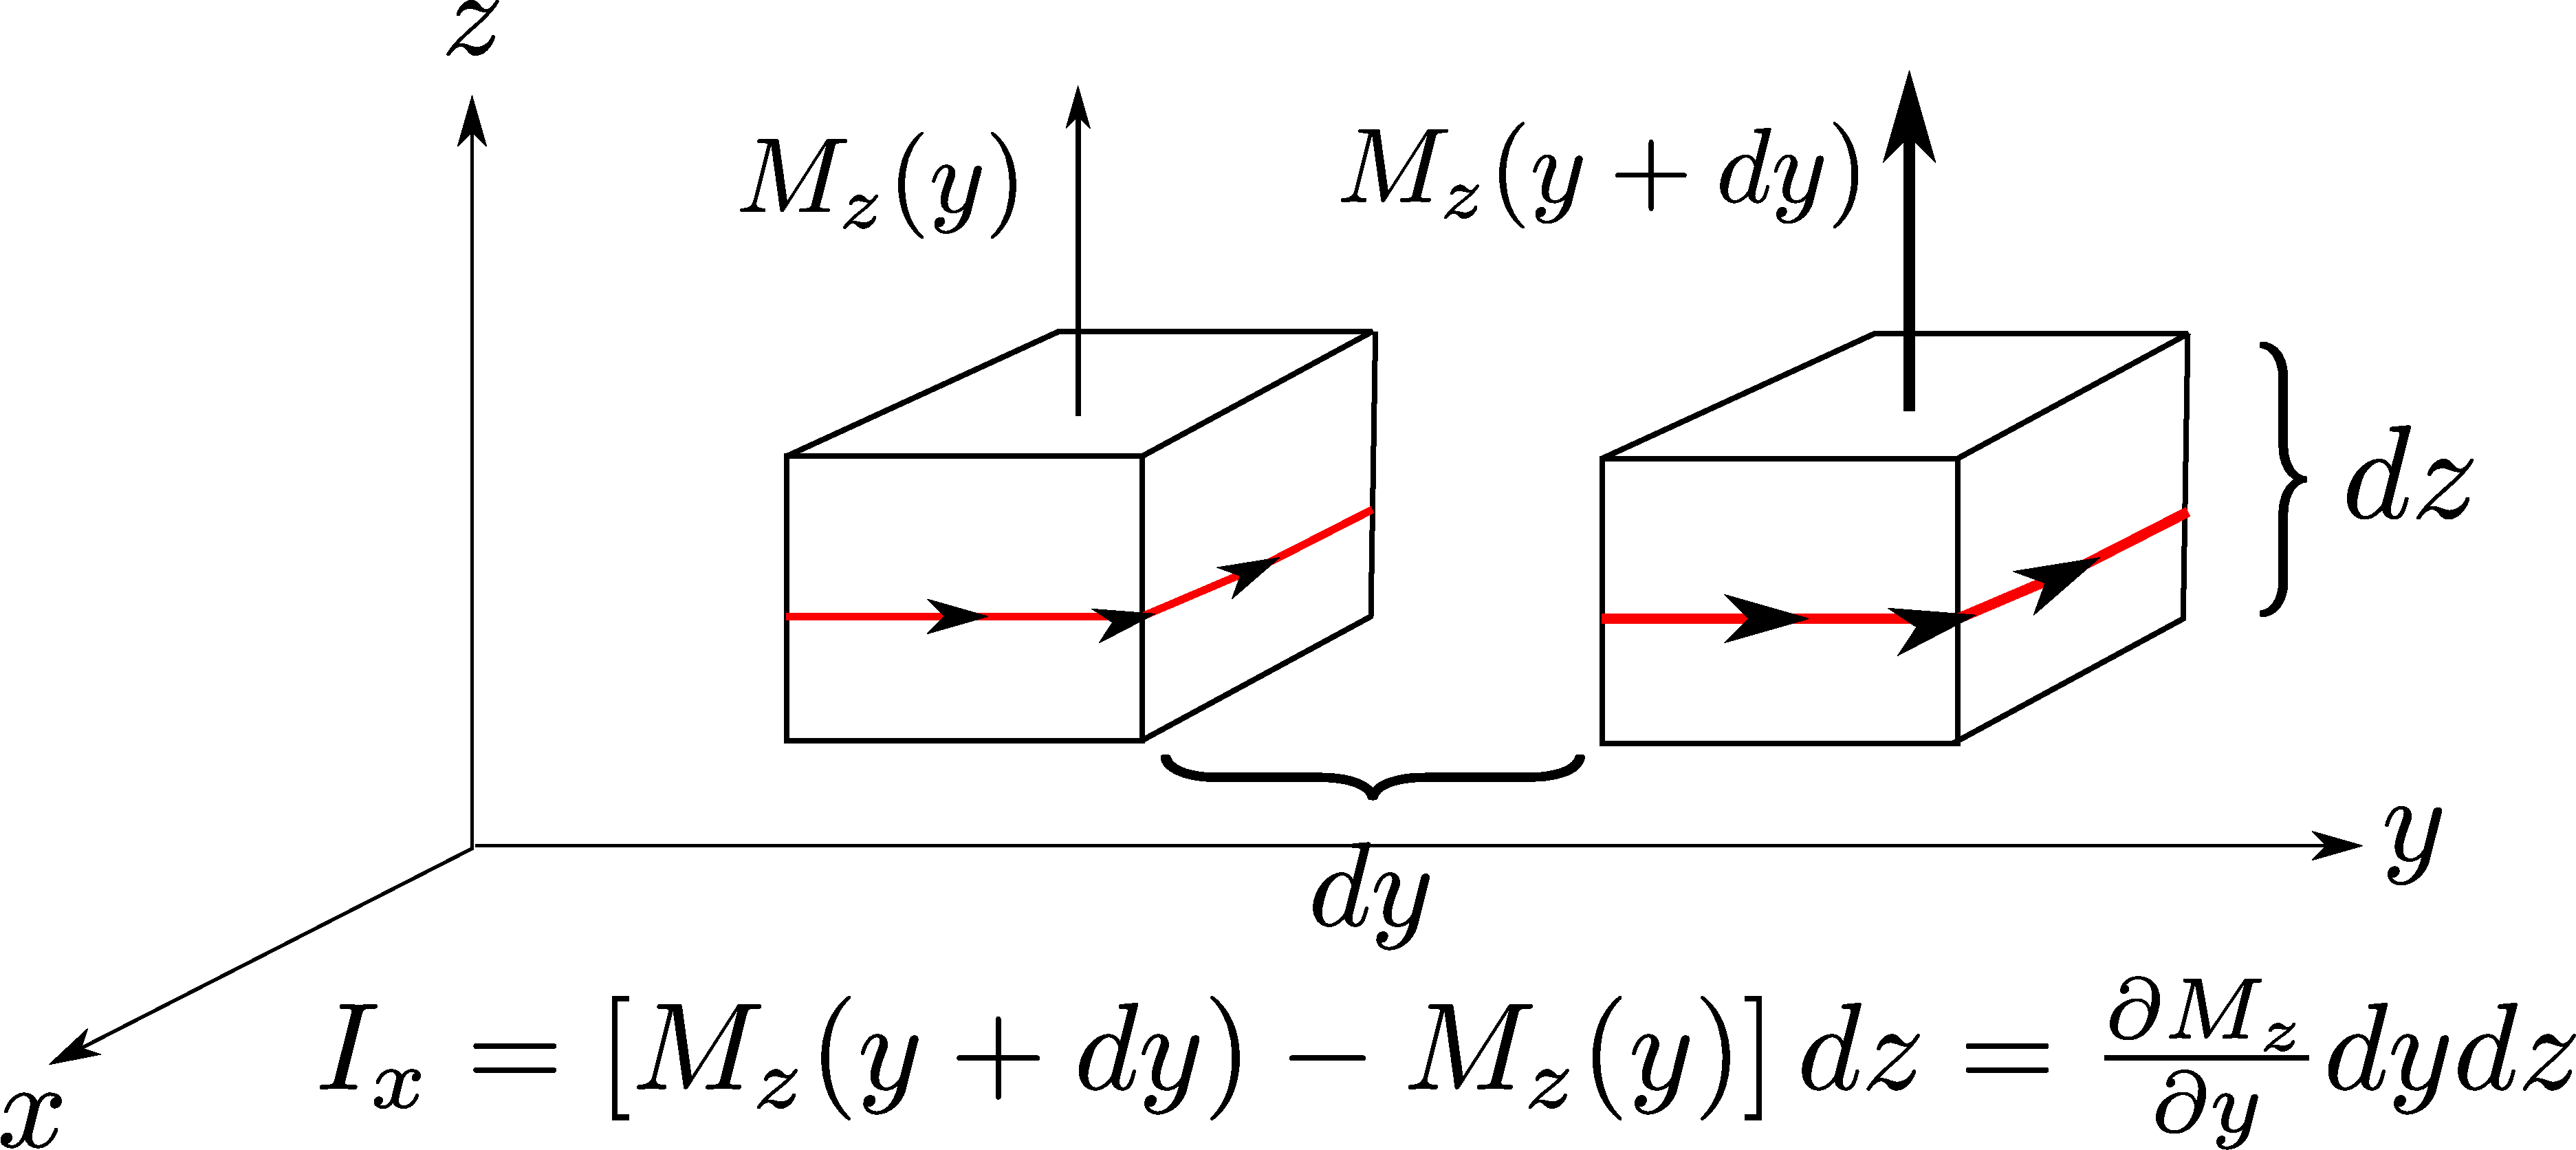
\psfig{file=fig/fig-corriente-magnetizacion-volumen.pdf,height=3cm,angle=0}}
\caption{Corrientes de magnetizaci'on de volumen y superficie. (Figura original gentileza de A. Maldonado) *** EDITAR, MEJORAR, EXPLICAR ***}
\label{fig-corriente-magnetizacion}
\end{figure}

Usando (\ref{AM1}) podemos calcular la contribuci'on de la magnetizaci'on a  la inducci'on magn'etica como:
\begin{eqnarray}
 B_i^{\rm M}&=&\varepsilon_{ijk}\partial_jA_k^{\rm M} \\
&=&\frac{\mu_0}{4\pi}\varepsilon_{ijk}\varepsilon_{kln}\int_V
M_l(x')\partial_j\partial'_n\frac{1}{\left\vert\vec{x}
-\vec{x}'\right\vert}dV'\\
&=&-\frac{\mu_0}{4\pi}\left(\delta_{il}\delta_{jn}-\delta_{in}
\delta_{jl}\right)\int_VM_l(x')\partial_j\partial_n\frac{1}{\left\vert\vec{x}
-\vec{x}'\right\vert}dV'\\
&=&\frac{\mu_0}{4\pi}\int_V\left[M_j(x')\partial_j\partial_i\frac{1}{
\left\vert\vec { x }-\vec{x}'\right\vert}-M_i(x')\partial_j\partial_j\frac{1}{
\left\vert\vec { x }-\vec{x}'\right\vert}\right]dV'\\
&=&\frac{\mu_0}{4\pi}\partial_i\left[\int_VM_j(x')\partial_j\frac{1}{
\left\vert\vec{x}-\vec{x}'\right\vert}dV'\right]-\frac{\mu_0}{4\pi}\int_V
M_i(x')\nabla^2\frac{1} {\left\vert\vec {x}-\vec{x}'\right\vert}dV'\\
&=&-\frac{\mu_0}{4\pi}\partial_i\left[\int_VM_j(x')\partial'_j\frac{1}{
\left\vert\vec{x}-\vec{x}'\right\vert}dV'\right]+\mu_0\int_V
M_i(x')\delta^{(3)}(\vec{x}-\vec{x}')dV',
\end{eqnarray}
de donde obtenemos:
\begin{equation}
 \boxed{\vec{B}^{\rm M}(x)=\mu_0\vec{M}(x)-\mu_0\vec\nabla\phi^*_{\rm M}(x),}
\label{BM}
\end{equation}
donde hemos definido el \textbf{potencial escalar de magnetizaci'on}\footnote{Note que 'este es un campo \textit{distinto} al potencial escalar magn'etico definido en la secci'on \ref{secpem}.}
\begin{equation}\marginnote{Potencial escalar de magnetizaci'on}
 \boxed{\phi^*_{\rm M}(x):=\frac{1}{4\pi}\int_VM_j(x')\partial'_j\frac{1}{
\left\vert\vec{x}-\vec{x}'\right\vert}dV'=\frac{1}{4\pi}
\int_V\frac{\vec{M}(x')\cdot (\vec{x}-\vec{x}')}{\left\vert\vec{x}-\vec{x}
'\right\vert^3} dV'. }
\end{equation}
En un sistema general existir'an, adem'as de la magnetizaci'on, corrientes
\textit{externas} (tambi'en llamadas \textit{libres} o \textit{de transporte}),
por lo que la inducci'on magn'etica total es dada por:
\begin{equation}
 \vec{B}(x)=\vec{B}^{\rm ext}(x)+\vec{B}^{\rm M}(x) .
\end{equation}
Usando (\ref{BS2}) y (\ref{BM}) encontramos finalmente una expresi'on para 
la inducci'on magn'etica macrosc'opica total en un medio magnetizado y con
corrientes externas:
\begin{equation}\marginnote{$\vec{B}$: corrientes externas + magnetizaci'on}
\boxed{ \vec{B}(x)=\frac{\mu_0}{4\pi}\int_V\frac{\vec{J}_{\rm ext}
(x')\times\left(\vec{x}-\vec{x}'\right)}{\left\vert\vec{x}-\vec{x}'\right\vert^3
} dV' +\mu_0\vec{M}(x)-\mu_0\vec\nabla\phi^*_{\rm M}(x).}
\label{BMG}
\end{equation}

\subsection{Excitaci'on magn'etica}\label{sec:defH}
Al calcular el rotor del campo definido en (\ref{BMG}), vea (\ref{ley-Ampere}),
encontramos:
\begin{equation}
 \vec\nabla\times\vec{B}=\mu_0\,\vec{J}_{\rm ext}
+\mu_0\vec\nabla\times\vec{M}.
\end{equation}
De aqu'i, podemos escribir
\begin{equation}
 \vec\nabla\times\left(\frac{1}{\mu_0}\vec{B}-\vec{M}\right)=\vec{J}_{
\rm ext}.
\end{equation}
Esto motiva definir la \textbf{excitaci'on magn'etica} (tambi'en llamada
\textbf{intensidad de campo magn'etico}):
\begin{equation}\marginnote{Excitaci'on magn'etica}\label{defH}
\boxed{\vec{H}(x):=\frac{1}{\mu_0}\vec{B}(x)-\vec{M}(x),}
\end{equation}
es decir,
\begin{equation}\label{HJM}
\vec{H}(x):=\frac{1}{4\pi}\int_V\frac{\vec{J}_{\rm ext}
(x')\times\left(\vec{x}-\vec{x}'\right)}{\left\vert\vec{x}-\vec{x}'\right\vert^3
} dV' -\vec\nabla\phi^*_{\rm M}(x) ,
\end{equation}
que satisface entonces la ``ley de Amp\`ere'',
\begin{equation}\marginnote{L. de Amp\`ere para $\vec{H}$}
 \boxed{\vec\nabla\times\vec{H}=\vec{J}_{\rm ext}} \label{rotHj}
\end{equation}
o, en su versi'on integral,
\begin{equation}
 \boxed{\oint_{\cal C}\vec{H}\cdot d\vec\ell=I_{\rm ext} .} \label{intHI}
\end{equation}
An'alogamente al caso del vector de desplazamiento el'ectrico $\vec{D}$, la
intensidad de campo magn'etico $\vec{H}$ es una cantidad 'util puesto que est'a
relacionada, a trav'es de la ecuaci'on (\ref{rotHj}), con las corrientes
externas del sistema, que son las corrientes que (en principio) pueden ser
manipuladas.

A partir de (\ref{HJM}) vemos que \textit{en regiones sin corrientes externas}, la excitaci'on magn'etica puede derivarse 'integramente del potencial escalar de magnetizaci'on\footnote{Compare con \eqref{Bgradphi}.},
\begin{equation}\marginnote{Si $\vec{J}_{\rm ext}=\vec{0}$}\label{HpM}
\vec{H}(x)= -\vec\nabla\phi^*_{\rm M}(x).
\end{equation}

\subsection{Condiciones de continuidad en interfaces}
\begin{figure}[!h]
\centerline{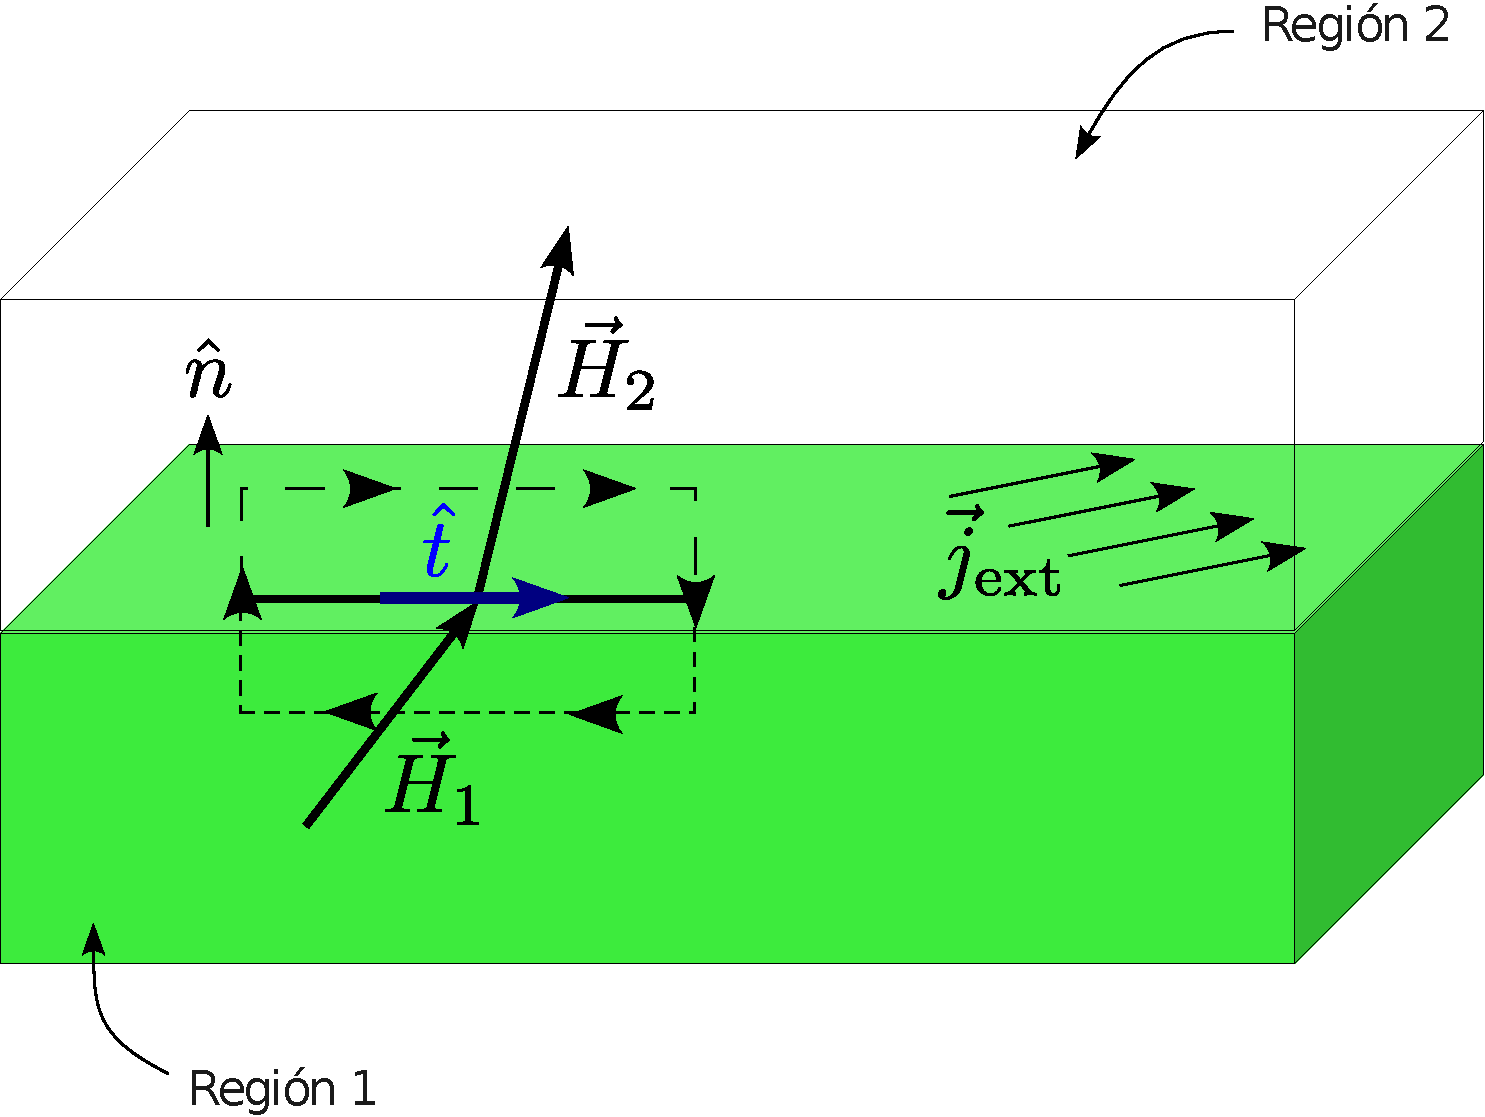
\psfig{file=fig/fig-condicion-borde-magnetica-01.pdf,height=5cm,angle=0}}
\caption{Condiciones de continuidad para $\vec{H}$ en una interface de dos
medios magn'eticos.}
\label{BM1}
\end{figure}
Al aplicar la ley de Amp\`ere (\ref{intHI}) al circuito de la figura \ref{BM1},
y considerando que
\begin{equation}\label{IextjS}
 I_{\rm ext}=\int_S\vec{J}_{\rm ext}\cdot d\vec{S}=\int_S\vec{J}_{\rm ext}\cdot
(\hat{n}\times\hat{t})\,dS=\vec{j}_{\rm ext}\cdot
(\hat{n}\times\hat{t})\,\ell=(\vec{j}_{\rm ext}\times\hat{n})\cdot\hat{t}\,\ell ,
\end{equation}
encontramos
\begin{equation}
 \boxed{\left(\vec{H}_2-\vec{H}_1\right)\cdot\hat{t}=(\vec{j}_{\rm
ext}\times\hat{n})\cdot\hat{t}} \label{Hint}
\end{equation}
o, equivalentemente
\begin{equation}
\boxed{\hat{n}\times\left(\vec{H}_2-\vec{H}_1\right)=\vec{j}_{\rm
ext}.}
\end{equation}
Note que en (\ref{IextjS}) el lado derecho contiene a la \textbf{densidad de corriente superficial externa} $\vec{j}_{\rm ext}$. En este caso puede considerarse que $\vec{J}_{\rm ext}=\vec{j}_{\rm ext}\delta(z)$, donde la superficie que limita las dos regiones est'a determinada por la condici'on $z=0$, siendo $z$ una coordenada normal a la superficie.

\textbf{Si no hay corrientes externas de superficie, entonces la componente \textit{tangencial} de la excitaci'on magn'etica cruza continuamente la interface}. En general, si
existen corrientes externas de superficie, la componente de la intensidad de
campo magn'etico paralela a $\vec{j}_{\rm ext}=j_{\rm ext}\,\hat{\jmath}$ cruzar'a continuamente la interface, mientras que la componente ortogonal tendr'a una discontinuidad de magnitud $j_{\rm ext}$. Esto puede verse directamente
de (\ref{Hint}) eligiendo $\hat{t}$ en la direcci'on y sentido de
$\vec{j}_{\rm ext}$, es decir, $\hat{t}=\hat{\jmath}$, obteniendo
\begin{equation}
 H_2^\parallel=H_1^\parallel,  \qquad H^\parallel:=\vec{H}\cdot\hat{\jmath},
\end{equation}
mientras que, eligiendo $\hat{t}=\hat{\jmath}\times\hat{n}$, encontramos
\begin{equation}
 H_2^\perp-H_1^\perp=j_{ext},  \qquad
H^\perp:=\vec{H}\cdot(\hat{\jmath}\times\hat{n}).
\end{equation}

Estas relaciones se complementan con aquella que se desprende del hecho que el campo magn'etico tiene siempre divergencia nula (independientemente del medio considerado). An'alogamente al caso el'ectrico, ver por ejemplo \eqref{saltoDn}, la ecuaci'on \eqref{divB} implica 
\begin{equation}\label{saltoBn}
\boxed{\left(\vec{B_2}-\vec{B_1}\right)\cdot\hat{n}=0,}
\end{equation}
es decir, la componente de $\vec{B}$ normal a la superficie es continua en la interface.

\subsection{Relaci'on constitutiva, susceptibilidad magn'etica}
An'alogamente al caso electrost'atico, se llama relaci'on constitutiva a la
relaci'on entre la magnetizaci'on de un material (la ``respuesta'' de 'este)
con el campo magn'etico existente, por ejemplo:
\begin{equation}
 \vec{M}=\vec{M}[\vec{H}].
\end{equation}
Esta relaci'on puede ser no-local, no-lineal, anis'otropa e inhomog'enea, y es usualmente inferida a partir de experimentos. Sin
embargo, muchos materiales pueden ser descritos por relaciones \textit{locales}. En
este caso puede parametrizarse la dependencia de la magnetizaci'on con la
intensidad magn'etica por medio de una serie de la forma
\begin{equation}
M_i(x)=M_i(H_j(x))=\left.M_i\right|_{\vec{H}=\vec{0}}
+\chi^{\rm m}_{ij}(x)H_j(x)+\chi^{\rm m}_{ijk}(x)H_j(x)H_k(x)+\cdots.
\end{equation}
%\begin{equation}
%M_i(x)=M_i(H_j(x))=\left.M_i\right|_{\vec{H}=\vec{0}}
%+H_j\left(\partial_jM_i\right)_{\vec{H}=\vec{0}}+\frac{1}{2}
%H_jH_k\left(\partial_j\partial_k M_i\right)_{\vec{H}=\vec{0}}+\cdots.
%\end{equation}
Para medios locales, \textit{lineales} y \textit{sin magnetizaci'on permanente}
($\left.M_i\right|_{\vec{H}=\vec{0}}=0$), la relaci'on se reduce a
\begin{equation}
 \boxed{M_i(x)=\chi^{\rm m}_{ij}(x)H_j(x),}
\end{equation}
donde $\chi^{\rm m}_{ij}$ es el \textbf{tensor de susceptibilidad magn'etica} del
material. En este caso, la inducci'on magn'etica adopta la forma
\begin{equation}
 \boxed{B_i(x)=\mu_{ij}(x)H_j(x)=\mu_0\,\kappa^{\rm m}_{ij}(x)H_j(x),}
\end{equation}
con el tensor de \textbf{permeabilidad magn'etica} $\mu_{ij}$ y el
tensor de \textbf{permeabilidad relativa} $\kappa^{\rm m}_{ij}$, definidos por
\begin{equation}
 \boxed{\mu_{ij}:=\mu_0\left(\delta_{ij}+\chi^{\rm
m}_{ij}\right)=\mu_0\kappa^{\rm m}_{ij}.}
\end{equation}
Finalmente, en el caso de medios locales, lineales e is'otropos, las
expresiones anteriores para la relaci'on constitutiva se reducen a
\begin{equation}
 \vec{M}(x)=\chi_{\rm m}(x)\vec{H}(x),
\end{equation}
\begin{equation}
 \vec{B}(x)=\mu(x)\vec{H}(x)=\mu_0\,\kappa_{\rm m}(x)\vec{H}(x),
\end{equation}
\begin{equation}
 \mu:=\mu_0\left(1+\chi_{\rm m}\right)=\mu_0\kappa_{\rm m}.
\end{equation}


\subsubsection{Ecuaci'on de Laplace para el potencial escalar de magnetizaci'on}
Como vimos en la secci'on \ref{sec:defH}, \textit{en regiones libres de corrientes externas} la excitaci'on magn'etica $\vec{H}$ es propocional al gradiente del potencial escalar de magnetizaci'on, ver (\ref{HpM}). Si adem'as el medio es \textit{lineal e is'otropo}, entonces $\vec{B}=\mu\vec{H}=-\mu\vec{\nabla}\phi^\ast_{\rm M}$. Finalmente, si adem'as el medio es \textit{homog'eneo}, encontramos, usando (\ref{divB}), que el potencial escalar de magnetizaci'on satisface la ecuaci'on de Laplace,
\begin{equation}
\nabla^2\phi^\ast_{\rm M}=0.
\end{equation}


\subsection{Paramagnetismo, diamagnetismo, ferromagnetismo}

\subsubsection{Diamagnetismo}
En este tipo de materiales $\vec{M}$ \textbf{tiene direcci'on opuesta a}  $\vec{H}$, por lo que $\chi_{\rm m}<0$ y $\kappa_{\rm m}<1$ y la inducci'on magn'etica $\vec{B}$ es \textbf{debilidata} (respecto al valor que asumir'ia en el vac'io, dada la misma distribuci'on de corrientes externas). Este tipo de materiales requiere que no existan \textit{momentos magn'eticos permanentes} significativos, de modo que la magnetizaci'on se deba principalmente a \textbf{corrientes inducidas}. Estas \textbf{corrientes inducidas generan momentos dipolares en sentido contrario al campo que las induce}, por lo que \textbf{la inducci'on magn'etica disminuye en el interior de un diamagneto}. En la mayor'ia de los casos de diamagnetismo la susceptibilidad magn'etica es independiente de la
temperatura y posee un valor muy peque\~no: $|\chi_{\rm m}|\lesssim 10^{-5}$. El
diamagnetismo es una propiedad general, es decir, que se presenta en todos los
materiales (siempre se producen peque\~nas corrientes inducidas), pero se dice
que un material es diamagn'etico si este efecto es el dominante, es decir,
cuando no existen otras fuentes de magnetizaci'on que reviertan la contribuci'on diamagn'etica.
Ejemplos de materiales diamagn'eticos: casi todas las substancias org'anicas,
metales nobles (oro, plata, cobre, mercurio, ...). Un caso extremo de
diamagnetismo es un \textbf{superconductor}, en el que la inducci'on magn'etica
es \textbf{anulada en su interior}, $\chi_{\rm m}=-1$ y $\kappa_{\rm m}=0$ (``diamagneto ideal'').

\subsubsection{Paramagnetismo}
 En este tipo de materiales la magnetizaci'on $\vec{M}$
tiene la misma direcci'on y sentido que $\vec{H}$. Equivalentemente $\vec{M}$
tiene la misma direcci'on y sentido que $\vec{B}$, de modo que
$\chi_{\rm m}>0$, $\kappa_{\rm m}>1$. Por esto, en un material paramagn'etico la inducci'on magn'etica $\vec{B}$ es \textbf{reforzada}. Este caso requiere que el material posea \textit{momentos magn'eticos permanentes}, que puedan anilearse con el campo magn'etico.
A la tendencia de los momentos magn'eticos a alinearse se
contrapone el ``desorden'' relacionado con las agitaciones t'ermicas del
material. Por esto, \textbf{en un material paramagn'etico $\chi_{\rm}$ disminuye a
medida que la temperatura aumenta}. Muchos materiales paramagn'eticos satisfacen
la \textbf{ley de Curie}: $\chi_{\rm}\propto 1/T$.
\begin{table}[h!]
\begin{center}
\begin{tabular}{c|c}
Material & $\chi_{\rm m}$ \\ \hline\hline
Aluminio & $2,1\times 10^{-5}$ \\
Cobre & $-0,98\times 10^{-5}$ \\
Oro & $-3,5\times 10^{-5}$ \\
Magnesio & $1.2\times 10^{-5}$ \\
Mercurio & $-2,8\times 10^{-5}$ \\
Plata & $-2,4\times 10^{-5}$ \\
Sodio & $0.84\times 10^{-5}$ \\
Titanio & $18.0\times 10^{-5}$ \\
Tungsteno & $7.6\times 10^{-5}$ \\
Hidr'ogeno (1 atm) & $-0,22\times 10^{-8}$ \\
Nitr'ogeno (1 atm) & $-0,67\times 10^{-8}$ \\
Ox'igeno (1 atm) & $193,5\times 10^{-8}$
\end{tabular}
\caption{Algunos materiales y sus susceptibilidades magn'eticas, a temperatura ambiente (Reitz-Milford).}
\end{center}
\end{table}

\subsubsection{Ferromagnetismo}

 En este tipo de materiales (t'ipicamente materiales que
contienen Fierro, Cobalto o N'iquel) \textbf{la magnetizaci'on no es
proporcional a la excitaci'on magn'etica}. Esto es algunas veces expresado
diciendo que la \textbf{susceptibilidad magn'etica efectiva} $\chi_{\rm m}:=M/H$ depende del valor del campo (y de otras variables, como por ejemplo de la temperatura), $\chi_{\rm m}=\chi_{\rm m}(T,\vec{H})$. El ferromagnetismo
requiere tambi'en que el material posea dipolos magn'eticos permanentes. Debido
a interacciones cu'anticas, los momentos magn'eticos de un ferromagneto se
ordenan \textit{espont'aneamente} (es decir, sin necesidad de campo magn'etico
externo), cuando la temperatura baja de un cierto valor cr'itico, llamada
temperatura de Curie, $T_{\rm C}$. En el cero absoluto de temperatura, todos los
momentos magn'eticos estar'ian alineados. A medida que la temperatura aumenta, el
desorden inducido por las vibraciones t'ermicas tiende a disminuir la
alineaci'on, pero sin conseguir
anular la magnetizaci'on total. Cuando la temperatura cruza la temperatura de
Curie, el sistema experimenta una transici'on de fase, y a partir de ese
momento se comporta como un paramagneto usual.
\begin{table}[h!]
\begin{center}
\begin{tabular}{c||c|c|c|c|c|c}
Material & Fe & Co & Ni & Gd & EuO & CrBr${}_3$  \\ \hline
$T_{\rm C}$ [K] & 1043 & 1393 & 631 & 290 & 69 & 37
\end{tabular}
\caption{Algunos materiales ferromagn'eticos y sus temperaturas de Curie 
\cite{Nolting}.}
\end{center}
\end{table}

T'ipicamente, los ferromagnetos poseen susceptibilidades
magn'eticas muy altas y \textbf{la magnetizaci'on que presentan depende de
su historia}, es decir, de c'omo hayan sido expuestos a campos externos. En
otras palabras, \textbf{dado un valor de la excitaci'on $\vec{H}$ el valor de $\vec{M}$
no es 'unico, sino que depende de c'omo se haya alcanzado el valor $\vec{H}$}.
Este fen'omeno es conocido como \textbf{hist'eresis}. El comportamiento de
hist'eresis t'ipico de un ferromagneto es ilustrado en la figura
\ref{fig-histeresis}.
\begin{figure}[!h]
\centerline{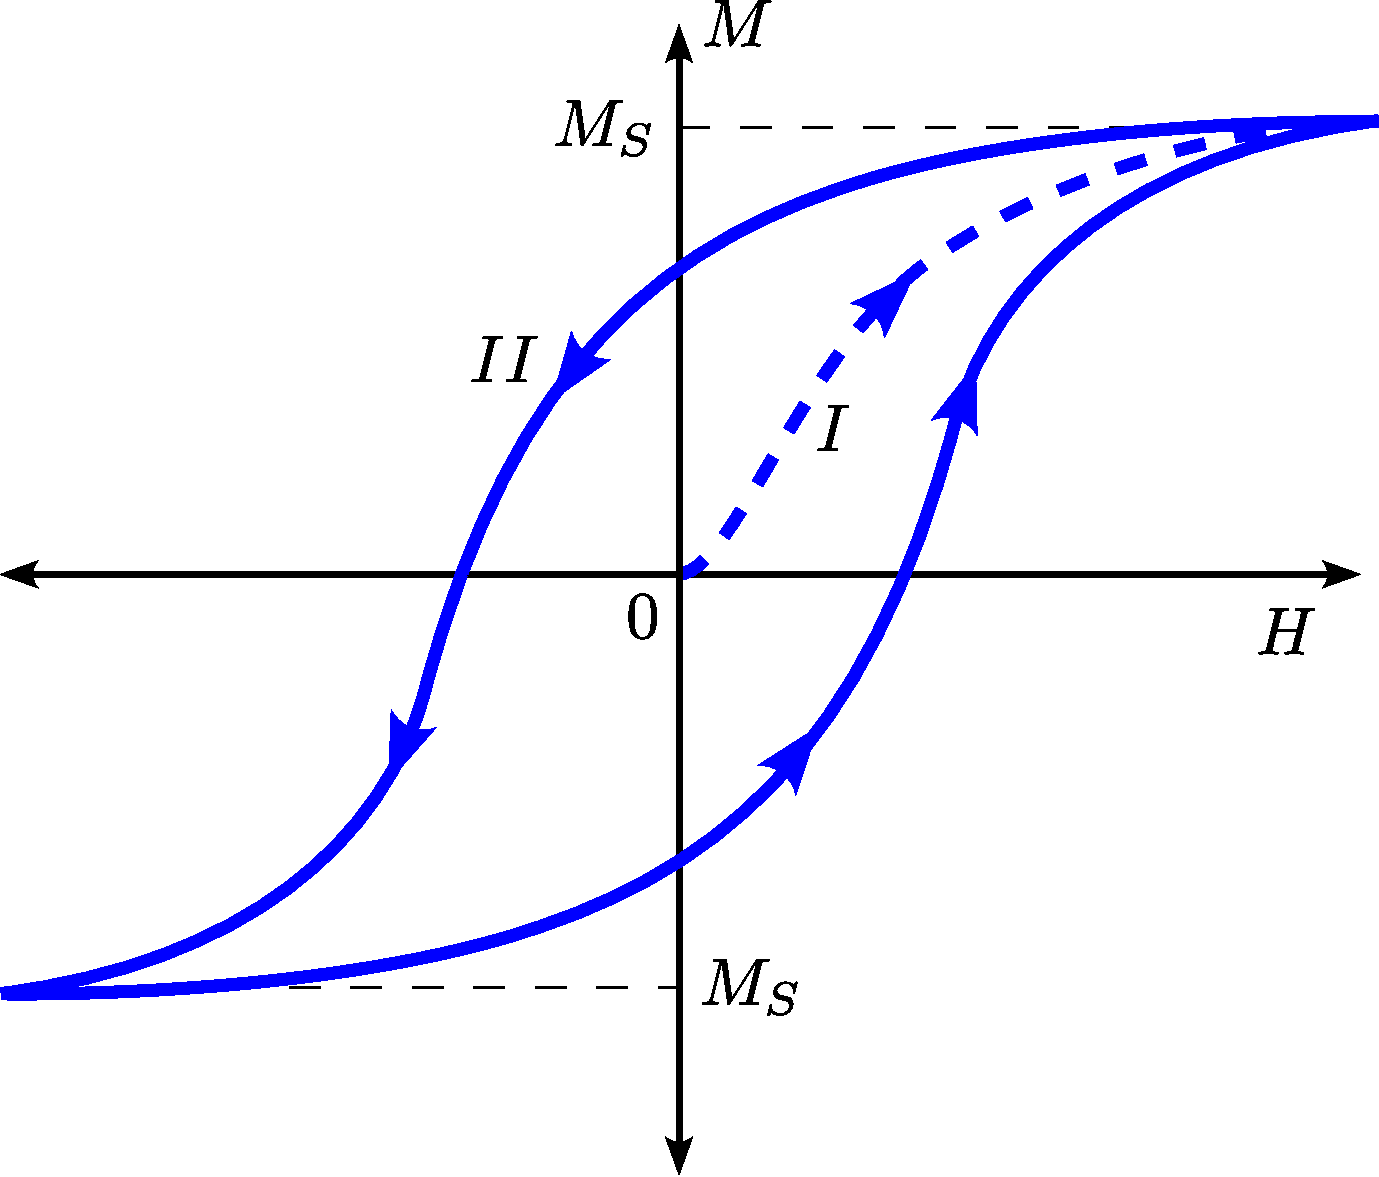
\psfig{file=fig/fig-histeresis-01.pdf,height=6cm,angle=0}}
\caption{Curva de hist'eresis t'ipica para un material ferromagn'etico.}
\label{fig-histeresis}
\end{figure}
Un material ferromagn'etico sin magnetizaci'on previa sometido a un campo $H$
se magnetiza siguiendo la curva I, llegando a una magnetizaci'on m'axima $M_S$ (``magnetizaci'on de saturaci'on"). 
Si luego se disminuye la intensidad de campo magn'etico el sistema se comienza
a demagnetizar, pero siguiendo la curva II, de modo que, incluso cuando el
campo $H$ es cero, el material conserva una magnetizaci'on no nula (magneto
permanente), llamada ``magnetizaci'on remanente''. Esta magnetizaci'on puede
ser anulada aplicando un campo en sentido inverso (intensidad de campo
``coercitivo''). La propiedad de hist'eresis est'a relacionada con la existencia
de \textbf{dominios magn'eticos}, que poseen un momento magn'etico macrosc'opico
no nulo y que requieren de energ'ia para reorientarse. La hist'eresis de los
ferromagnetos es usada en la fabricaci'on de \textbf{dispositivos de memoria}, en los
que la informaci'on es codificada en la orientaci'on del momento magn'etico de
los dominios, que permanece indefinidamente hasta que campos externos sean
usados para cambiar su estado.
\newpage
\chapter{Electrodin'amica}

\section{Ley de inducci'on de Faraday}

Faraday\footnote{Michael Faraday (1791-1867): f'isico y qu'imico brit'anico. Ver \url{http://es.wikipedia.org/wiki/Michael_Faraday}.} encontr'o experimentalmente (1831) que \textit{si el flujo magn'etico a trav'es de una espira cerrada var'ia en el tiempo, se induce una corriente sobre una espira}. Si el flujo es constante, se observa que la corriente desaparece. La \textbf{ley de Faraday} se escribe como
\begin{equation}\label{faraday}
\varepsilon_{\rm ind}=-K\frac{d\phi}{dt},
\end{equation}
donde $\varepsilon_{\rm ind}$ es la fuerza electromotriz (f.e.m.) \textit{inducida} en la espira. El signo menos describe la direcci'on de la corriente inducida, dada por la \textbf{ley de Lenz}. Aqu'i $K$ es una constante que depende del sistema de unidades usado. En el Sistema Internacional es una cantidad adimensional, que determinaremos m'as adelante.

En t'erminos de campos, se genera un campo el'ectrico $\vec{E}$ que es el que hace mover las cargas en la espira, es decir,
\begin{equation}
\oint_{\cal\partial S}\vec{E}\cdot d\vec{\ell}=\varepsilon_{\rm ind}.
\end{equation}
Con esto, podemos escribir (\ref{faraday}) como
\begin{equation}
\oint_{\cal \partial S}\vec{E}\cdot d\vec{\ell}=-K\frac{d\ }{dt}\int_S\vec{B}\cdot
d\vec{S}.
\end{equation}
En general, la superficie puede variar en el tiempo. Si 'este \textit{no} es el caso, y $S$
es constante, entonces podemos deducir que
\begin{equation}\label{ley-faraday0}
\vec\nabla\times\vec{E}=-K\frac{\partial\vec{B}}{\partial t}.
\end{equation}
Considere ahora el caso en que la espira se mueve \textit{r'igidamente}, es decir, que la velocidad de los puntos de la espira es independiente de la posici'on (puede, sin embargo, depender del tiempo).
Entonces el cambio del flujo por la superficie, entre los tiempos $t$ y $t+dt$, puede calcularse como sigue:
\begin{eqnarray}
 d\Phi &=& \Phi(t+dt)-\Phi(t)\\
&=&
\int_{S(t+dt)}B_i(\vec{x}+\vec{v}dt,t+dt)dS_i-\int_{S(t)}B_i(\vec{x},t)dS_i\\
&=&\int_{S(t+dt)}\left[B_i(\vec{x},t)+dt\,v_j\,\partial_jB_i(\vec{x},
t)+dt\,\partial_tB_i(\vec{x},t)\right ] dS_i-\int_{S(t)}B_i(\vec{x},t)dS_i\\
&=&\int_S\left[B_i(\vec{x},t)+dt\,v_j\,\partial_jB_i(\vec{x},
t)+dt\,\partial_tB_i(\vec{x},t)\right ] dS_i-\int_SB_i(\vec{x},t)dS_i\\
&=&dt\int_S\left[v_j\,\partial_jB_i(\vec{x},t)+\partial_tB_i(\vec{x},t)\right
] dS_i.
\end{eqnarray}
En la pen'ultima igualdad usamos el hecho que el elemento de superficie $dS_i$ sobre la superficie $S(t)$ y $S(t+dt)$ son iguales, ya que la superficie se mueve r'igidamente (es decir, con igual velocidad en cada punto). As'i obtenemos que
\begin{equation}\label{dPhidt0}
 \frac{d\Phi}{dt}=\int_S\left[v_j\,\partial_jB_i(\vec{x},t)+\partial_tB_i(\vec
{x},t)\right] dS_i.
\end{equation}
Usamos ahora la identidad
\begin{equation}
\varepsilon_{ijk}\partial_j(\varepsilon_{klm}B_lv_m)\equiv
v_j(\partial_jB_i)-v_i(\partial_jB_j),
\end{equation}
y la ley (\ref{divB}) (que suponemos v'alida incluso en el caso din'amico) para reescribir (\ref{dPhidt0}) como
\begin{eqnarray}
 \frac{d\Phi}{dt}&=&\int_S\left[\partial_tB_i+\varepsilon_{ijk}
\partial_j(\varepsilon_{klm} B_lv_k)\right] dS_i \\
&=& \int_S\partial_tB_i\, dS_i +\oint_{\partial S}\varepsilon_{ijk}
B_jv_k\,dx_i 
\end{eqnarray}
o, en notaci'on vectorial, 
\begin{equation}\label{dFlujodt}
  \frac{d\Phi}{dt}=\int_S\frac{\partial\vec{B}}{\partial
t}\cdot d\vec{S}-\oint_{\partial
S}\left(\vec{v}\times\vec{B}\right)\cdot d\vec{\ell}.
\end{equation}
Apliquemos estos resultados para comparar la descripci'on, respecto a dos sistemas de referencia inerciales (SRI's), del fen'omeno de inducci'on de corriente en una espira debido a la variaci'on de flujo magn'etico. Primero, en el SRI $K$ en el que la espira est'a en reposo y el magneto se mueve tenemos que en cada punto del espacio el campo magn'etico $\vec{B}$ depender'a del tiempo, por lo que se inducir'a un campo el'ectrico de acuerdo a (\ref{ley-faraday0}). Este campo el'ectrico ejercer'a una fuerza $\vec{F}_q=q\vec{E}$ sobre una carga $q$ en la espira, que consideraremos inicialmente en reposo. 

Por otro lado, en un SRI $K'$ con velocidad relativa $\vec{v}$ respecto a $K$ (de modo que en $K'$ el magneto est'a en reposo) la corriente inducida es debido al movimiento de la espira. Si en este SRI el campo magn'etico es $\vec{B}'(x)$, no existe campo el'ectrico inducido puesto que $\partial\vec{B}'/\partial t=\vec{0}$. En este SRI la corriente inducida se describe 'integramente debido a la fuerza de Lorentz ejercida por el campo magn'etico sobre las cargas en la espira, que ahora se mueven con velocidad $-\vec{v}$. La fuerza que act'ua sobre la carga es ahora $\vec{F}'_q=-q\vec{v}\times\vec{B'}$. Adem'as, la f.e.m. est'a dada, usando el resultado (\ref{dFlujodt}) aplicado a este caso, as'i como la ley de Faraday (\ref{ley-faraday0}), por 
\begin{equation}
\varepsilon'_{\rm ind}=-K\oint_{\partial S}\left(\vec{v}\times\vec{B}'\right)\cdot d\vec{\ell}.
\end{equation}

 Ya que $K$ y $K'$ son SRI's, la aceleraci'on, y por tanto la fuerza que act'ua sobre la carga (inicialmente en reposo en $K$), son necesariamente iguales. De lo anterior, es decir $\vec{F}_q=\vec{F}'_q$, vemos que esto s'olo es posible si el campo inducido es dado por
 \begin{equation}\label{EvBp}
\vec{E}=-\vec{v}\times\vec{B'}.
\end{equation}
Adem'as, la f.e.m. debe ser la misma, ya que la corriente inducida lo es, por lo que
\begin{align}
\varepsilon_{\rm ind} &= \varepsilon'_{\rm ind}, \\
\oint_{\partial S}\vec{E}\cdot d\vec{\ell} &=-K\oint_{\partial S}\left(\vec{v}\times\vec{B}'\right)\cdot d\vec{\ell}.
\end{align}
Usando ahora (\ref{EvBp}) en el lado izquierdo obtenemos
\begin{equation}
-\oint_{\partial S}\left(\vec{v}\times\vec{B'}\right)\cdot d\vec{\ell} =-K\oint_{\partial S}\left(\vec{v}\times\vec{B}'\right)\cdot d\vec{\ell}.
\end{equation}
Esta relaci'on implica que la constante $K$ debe tener, en el Sistema Internacional de Unidades, el valor $K=1$. 

De esta forma, la ley de Faraday adopta la forma
\begin{equation}
\boxed{\oint_{\cal\partial S}\vec{E}\cdot d\vec{\ell}=-\frac{d\ }{dt}\int_S\vec{B}\cdot
d\vec{S}}
\end{equation}
o, en forma diferencial:
\begin{equation}
\boxed{\vec\nabla\times\vec{E}=-\frac{\partial\vec{B}}{\partial t}.}
\label{ley-faraday}
\end{equation}

%\subsection{Autoinducci'on}
%\begin{equation}
% L:=\frac{d\Phi}{dI}
%\end{equation}
%\begin{equation}
% \varepsilon_{\rm ind}=-L\frac{dI}{dt}
%\end{equation}


\subsection{Energ'ia del campo magn'etico}

Consideremos ahora una espira por la que circula una corriente $I$ y el campo magn'etico \textit{que ella misma produce}. Si $I$ no var'ia en el tiempo, no existe fem inducida ya que el flujo magn'etico por la espira permanece constante (suponemos una espira fija, en reposo). Calcularemos la energ'ia necesaria para cambiar la corriente $I$ y el correspondiente campo magn'etico $\vec{B}$ en una peque\~na cantidad. Durante el intervalo de tiempo $dt$ en que la corriente cambia en $dI$ y el campo magn'etico en $d\vec{B}$, se genera un campo el'ectrico inducido y su correspondiente fem $\varepsilon$ (que en general se superponen al campo y fem que mantien'ian la corriente $I$ fluyendo originalmente). Este campo inducido ``intenta reducir'' el cambio de la corriente. Para esto, el campo realiza trabajo sobre las cargas en movimiento en la espira. 
%Calcularemos la energ'ia transferida a las cargas que se ponen en movimiento para formar la corriente inducida en una espira, debido a la inducci'on de Faraday. Para esto, consideraremos una espira que forma una curva cerrada $\cal C$ por la que circula una corriente inducida $I$. 

Dividiremos la curva en elementos de longitud $d\vec{\ell}=d\ell \,\hat{t}$, en los que existe una carga $dq=\lambda d\ell$. El vector unitario $\hat{t}$ est'a definido de modo que $d\vec{\ell}$ tiene la orientaci'on standard respecto al vector normal $\hat{n}$ a la superficie que encierra la espira. El campo el'ectrico $\vec{E}$ ejerce trabajo sobre las cargas $dq$. En un intervalo de tiempo $dt$ el trabajo realizado sobre las cargas $dq$ es entonces 
\begin{align}
dq\,\vec{E}\cdot d\vec{\ell} &= (\lambda d\ell) \vec{E}\cdot (\vec{v}\,dt) \\
&= (\lambda d\ell) \vec{E}\cdot (v\,\hat{t})\,dt \\
&= (\lambda v) \vec{E}\cdot (d\ell\,\hat{t})\,dt \\
&= I(\vec{E}\cdot d\vec{\ell})\,dt.
\end{align}
Aqu'i hemos identificado la corriente $I=\lambda v$ sobre la espira, y tomado en cuenta que $\vec{v}=v\hat{t}$. Por lo tanto, el trabajo total realizado por el campo sobre las cargas de la espira, en el intervalo de tiempo $dt$, es dado por
\begin{align}
dW &= \oint_{\cal C}dq\,\vec{E}\cdot d\vec{\ell} \\
&= I\oint_{\cal C}(\vec{E}\cdot d\vec{\ell})\,dt \\
&= I\varepsilon\,dt \\
&= -I\frac{d\Phi}{dt}\,dt \\
&= -I\,d\Phi.
\end{align}

A partir de este resultado vemos que la energ'ia (proveniente de fuentes externas) necesaria para cambiar el flujo magn'etico en una cantidad $d\Phi$, en un sistema con una corriente $I$ es dada por
\begin{equation}\label{dWIdP}
 \boxed{dU=I\,d\Phi.}
\end{equation}
En otras palabras, \textit{un cambio en el valor de la intensidad de campo $\vec{B}$ requiere invertir energ'ia}. En cierto sentido, la ley de Faraday establece una cierta ``inercia'' en el campo magn'etico, ya que un sistema de cargas y campos tiende a ``resistirse'' al cambio del valor del campo (y su flujo). 
Esto implica adem'as que \textit{es necesario asociar una energ'ia a una cierta configuraci'on de campos y corrientes}, puesto que es necesario invertir energ'ia para establecer estas corrientes y sus campos asociados. Para evaluar esta energ'ia, reescribiremos (\ref{dWIdP}) usando (\ref{PAdx}): la energ'ia $\delta U$ necesaria para variar el potencial vectorial $\vec{A}(x)$ de un sistema de corrientes y campo magn'etico en $\delta\vec{A}(x)$ es dada por
\begin{align}
 \delta U &= I\oint_{\cal C}\delta\vec{A}\cdot d\vec{\ell} \\
 &= \oint_{\cal C}\delta\vec{A}\cdot Id\vec{\ell} \\
 &= \int_V\delta\vec{A}\cdot \vec{J}_{\rm ext}\,dV. \label{WdAJ}
\end{align}
En el 'ultimo paso hemos usado la relaci'on (\ref{IdxJdV}) para reescribir la energ'ia en t'erminos de una integral de volumen de la densidad de corriente. Note que la corriente inducida es en general corriente ``externa'' o de ``conducci'on'', por lo que hemos explicitado en el 'ultimo t'ermino la densidad de corrientes externas $\vec{J}_{\rm ext}$. Adem'as, usando la ley de Amp\`ere para la excitaci'on magn'etica (\ref{rotHj}), podemos escribir
\begin{align}
 \delta U 
&= \int_{V'} \delta A_i\,\varepsilon_{ijk}\left(\partial_jH_k\right)\,dV \\
&= \varepsilon_{ijk}\int_{V'} \left[\partial_j(H_k\delta A_i)-H_k(\partial_j\delta A_i)\right]dV\\
&= \varepsilon_{ijk}\oint_{\partial V'}H_k\delta
A_i\,dS_j-\varepsilon_{ijk}\int_{V'}H_k(\partial_j\delta A_i)\,dV\\
&= 0+\int_{V'} H_k\,\varepsilon_{kji}(\partial_j\delta A_i)\,dV\\
&= \int_{V'} H_k\,\delta B_k\,dV.
\end{align}
Aqu'i hemos extendido el dominio de integraci'on a un volumen $V'\to R_3$, es decir, a todo el espacio, usado el teorema de Gauss y considerado que la integral de superficie se anula en el infinito. Con esto, obtenemos la siguiente expresi'on para la \textit{energ'ia requerida para cambiar la inducci'on magn'etica de un sistema en $\delta{\vec B}(x)$}:
\begin{equation}
 \boxed{\delta U=\int_{R^3} \vec{H}(x)\cdot \delta\vec{B}(x)\,dV.}\label{dUB}
\end{equation}
Note la similitud entre las expresiones (\ref{WdAJ}) y (\ref{dUB}) con los resultados (\ref{Wdiel1}) y (\ref{dUE}) para la energ'ia almacenada por un campo el'ectrico, respectivamente.

*** Agregar comentario energ'ia y 'area bajo la curva de gr'afico $H$ v/s $B$ ***

Similarmente a lo discutido en el caso el'ectrico, la \textit{energ'ia total requerida para aumentar el campo magn'etico de un sistema desde cero hasta un valor final $\vec{B}$} es 
\begin{equation}
 U=\int_0^1\int_{R^3} \lambda \, \vec{H}(x)\cdot \delta\vec{B}_\lambda(x)\,dV,
\end{equation}
donde $\vec{B}_\lambda(x)$ es el valor de la inducci'on magn'etica correspondiente al caso en que la excitaci'on magn'etica tiene un valor $\vec{H}_\lambda(x)$ igual a una fracci'on $\lambda$ de la excitaci'on magn'etica final, es decir, $\vec{H}_\lambda (x)=\lambda\vec{H}_\lambda (x)$ .

En el caso de un \textit{medio magn'etico lineal}, tendremos que $\vec{B}_\lambda (x)=\lambda\, \vec{B}(x)$ y por lo tanto $\delta\vec{B}_\lambda (x)=d\lambda\,
\vec{B}(x)$, y entonces
\begin{equation}\label{UHB}
 \boxed{U=\frac{1}{2}\int_{R^3} \vec{H}(x)\cdot\vec{B}(x)\,dV }
\end{equation}
o, alternativamente, 
\begin{equation}
 \boxed{U=\frac{1}{2}\int_{R^3} \vec{A}\cdot \vec{J}\,dV.}
\end{equation}

Usando (\ref{UHB}) podemos escribir la energ'ia almacenada en un sistema de campo magn'etico (y corrientes) como la integral de una \textbf{densidad de energ'ia magn'etica}
\begin{equation}
 \boxed{U=\int_{R^3} u_B(x)\,dV, \qquad u_B(x):=\frac{1}{2}\vec{H}(x)\cdot\vec{B}(x).}
\end{equation}
En el caso particular de medio lineales e is'otropos la densidad de energ'ia magn'etica se reduce a
\begin{equation}
 u_B(x)=\frac{\mu}{2}\vec{H}^2(x)=\frac{1}{2\mu}\vec{B}^2(x).
\end{equation}


\subsection{Fuerzas y torques sobre circuitos magn'eticos}
%\begin{equation}
%\boxed{F_i=-\left(\frac{\partial U}{\partial x_i}\right) ,} \label{FQB}
%\end{equation}
%
%\begin{equation}
% \boxed{\vec{\tau}\cdot\hat{n}=-\left(\frac{\partial U}{\partial\theta}\right).}
%\end{equation}

\section{Ecuaciones de Maxwell}
Hasta el momento,
\begin{align}
\vec\nabla\cdot\vec{D} & =\rho ,\label{cmax1}\\
\vec\nabla\cdot\vec{B}  & =0 ,\label{cmax2}\\
\vec\nabla\times\vec{H}  & =\vec{J} ,\label{cmax3}\\
\vec\nabla\times\vec{E}  & =-\frac{\partial\vec{B}}{\partial t} .\label{cmax4}
\end{align}
Note que aqu'i hemos suprimido, para no recargar la notaci'on, la designaci'on ``${\rm ext}$'' en la densidad de carga y corriente externa.

Vemos que (\ref{cmax3}) implica $\vec\nabla\cdot\vec{J}=0$, que es una condici'on que \textit{no es v'alida en general}, sino que s'olo en los casos, de acuerdo a (\ref{eccont}), en que ${\partial\rho}/{\partial t}=0$. Esto lleva a pensar que (al menos) la ecuaci'on (\ref{cmax3}) no es v'alida en el caso din'amico m'as general en el que las densidades de carga y corriente, y por lo tanto los campos el'ectricos y magn'eticos, var'ian en el tiempo.

Maxwell\footnote{James Clerk Maxwell (1831-1879): F'isico escoc'es. Ver \url{http://es.wikipedia.org/wiki/James_Clerk_Maxwell}.} (1861) generaliz'o la ecuaci'on (\ref{cmax3}) de modo que sea compatible con (\ref{cmax1}) y la ley de conservaci'on de la carga el'ectrica,
es decir, con la ecuaci'on de continuidad (\ref{eccont}). Usando (\ref{cmax1}), que suponemos por tanto v'alida en el caso general, podemos escribir (\ref{eccont}) como
\begin{eqnarray}
 0&=&\frac{\partial\rho}{\partial t}+\vec{\nabla}\cdot\vec{J}\\
&=& \frac{\partial\ }{\partial
t}\left(\vec\nabla\cdot\vec{D}\right)+\vec{\nabla}\cdot\vec{J}\\
&=& \vec\nabla\cdot\left[\frac{\partial\vec{D}}{\partial t}
+\vec{J}\right].
\end{eqnarray}
De aqu'i vemos que en el caso de corrientes generales (no-est'aticas), $\vec{J}$ tiene divergencia no nula, pero la combinaci'on $\vec{J}+{\partial\vec{D}}/{\partial t}$ \textit{siempre tiene divergencia nula}. A partir de esta observaci'on, Maxwell \textit{postul'o} que el lado derecho de la ecuaci'on (\ref{cmax3}) deb'ia ser reemplazada por la combinaci'on $\vec{J}+{\partial\vec{D}}/{\partial t}$. En otras palabras, Maxwell postul'o que a la densidad de corriente deber'ia agregarse el t'ermino ${\partial\vec{D}}/{\partial t}$, llamado \textit{corriente de desplazamiento}.

Con esto, las ecuaciones de Maxwell adoptan la forma:
\begin{align}
\vec\nabla\cdot\vec{D} & =\rho ,\label{max1}\\
\vec\nabla\cdot\vec{B}  & =0 ,\label{max2}\\
\vec\nabla\times\vec{H}  & =\vec{J}+\frac{\partial\vec{D}}{\partial
t} ,\label{max3}\\
\vec\nabla\times\vec{E}  & =-\frac{\partial\vec{B}}{\partial t}.\label{max4}%
\end{align}

Estas ecuaciones son completadas con las relaciones constitutivas entre
$\vec{E}$ y $\vec{D}$, y entre $\vec{B}$ y $\vec{H}$, as'i como con la expresi'on de la (densidad de) fuerza de Lorentz:
\begin{equation}
\vec{f}=\rho\vec{E}+\vec{J}\times\vec{B}.
\end{equation}

\section{Conservaci'on de la energ'ia y Vector de Poynting}\label{sec:energia}
Calculamos el producto escalar de $\vec{E}$ con la ecuaci'on (\ref{max3}).
Usando notaci'on tensorial, obtenemos:
\begin{equation}
 E_i\frac{\partial D_i}{\partial t}
-E_i\,\varepsilon_{ijk}\partial_jH_k+E_iJ_i=0.
\end{equation}
An'alogamente, el producto escalar entre $\vec{H}$ con la ecuaci'on
(\ref{max4}) implica,
\begin{equation}
H_i\frac{\partial B_i}{\partial t} +H_i\varepsilon_{ijk}\partial_jE_k=0.
\end{equation}
Sumando estas ecuaciones, obtenemos
\begin{align}
0 &= E_i\frac{\partial D_i}{\partial t}+H_i\frac{\partial B_i}{\partial t}
-E_i\varepsilon_{ijk}\partial_jH_k+E_iJ_i+H_i\varepsilon
_{ijk}\partial_jE_k\\
 &= E_i\frac{\partial D_i}{\partial t}+H_i\frac{\partial B_i}{\partial
t}+E_iJ_i+\varepsilon_{ijk}\left(H_i\partial_jE_k-E_i\partial_jH_k\right)\\
 &= E_i\frac{\partial D_i}{\partial t}+H_i\frac{\partial B_i}{\partial
t}+E_iJ_i+\varepsilon_{ijk}\left(H_i\partial_jE_k+E_k\partial_jH_i\right)\\
 &= E_i\frac{\partial D_i}{\partial t}+H_i\frac{\partial B_i}{\partial
t}+E_iJ_i+\partial_j(\varepsilon_{jki}E_kH_i).
\end{align}
En resumen, las ecuaciones de Maxwell (\ref{max3}) y (\ref{max4}) implican que
\begin{equation}
\boxed{\vec{E}\cdot\frac{\partial \vec{D}}{\partial
t}+\vec{H}\cdot\frac{\partial\vec{B}}{\partial t}+
\vec\nabla\cdot(\vec{E}\times\vec{H})
+\vec{E}\cdot\vec{J}=0.} \label{cEem0}
\end{equation}
Es 'util definir el \textit{vector de Poynting}\footnote{John Henry Poynting (1852-1914): f'isico ingl'es. Ver \url{http://es.wikipedia.org/wiki/John_Henry_Poynting} $\leftarrow$ \textbf{Esta p'agina podr'ia ser mejorada considerablemente, traduciendo la correspondiente en ingl'es!. ?`voluntarios?}} como
\begin{equation}\label{defPoy}\marginnote{Vector de Poynting}
\boxed{\vec{S}:=\vec{E}\times\vec{H}.}
\end{equation}
En un peque\~no intervalo de tiempo $dt$ los campos cambian (en cada punto fijo del espacio) en las peque\~nas cantidades dadas por $d\vec{D}=dt\,({\partial \vec{D}}/{\partial t})$ y
$d\vec{B}=dt\,({\partial \vec{B}}/{\partial t})$. Entonces podemos escribir
\begin{equation}
\vec{E}\cdot
d\vec{D}+\vec{H}\cdot d\vec{B}+\vec\nabla\cdot\vec{S}\,dt+\vec{E}\cdot\vec{J}\,
dt=0,
\end{equation}
que, integrado en un volumen $V$ conduce a 
\begin{equation}
\boxed{\int_V\left[\vec{E}\cdot d\vec{D}+\vec{H}\cdot
d\vec{B}\right]dV+\oint_{\partial V}
\vec{S}\cdot d\vec{S}\,dt+\int_V\vec{E}\cdot\vec{J}\,
dVdt=0.} \label{cEem1}
\end{equation}
Identificamos el 'ultimo t'ermino como el \textbf{trabajo realizado por el campo el'ectrico sobre las corrientes}, es decir, la energ'ia transferida del campo a las cargas (o viceversa, dependiendo del signo). Adem'as, de acuerdo a los resultados previos (\ref{dUE}) y (\ref{dUB}) la primera integral puede interpretarse como el \textbf{cambio total de la energ'ia almacenada en forma de campo el'ectrico y magn'etico}, en el volumen $V$. Finalmente, interpretamos la integral de superficie como la \textbf{energ'ia electromagn'etica neta que fluye a trav'es de la superficie $\partial V$}. En otras palabras, interpretamos el vector de Poynting como la \textit{densidad de flujo de energ'ia} electromagn'etica (la energ'ia electromagn'etica transportada por unidad de superficie y unidad de tiempo). De esta forma, (\ref{cEem1}) es una \textit{ecuaci'on de balance (o conservaci'on) de la energ'ia}.

En el caso particular de \textit{medios lineales, no disipativos, y con susceptibilidades
independientes del tiempo}, es decir, tales que
\begin{equation}
D_i=\varepsilon_{ij}E_j, \qquad \partial_t\varepsilon_{ij}=0, \qquad \varepsilon_{ij}=\varepsilon_{ji},
\end{equation}
\begin{equation}
B_i=\mu_{ij}H_j, \qquad \partial_t\mu_{ij}=0, \qquad \mu_{ij}=\mu_{ji},
\end{equation}
podemos reescribir:
\begin{equation}
 \vec{E}\cdot\frac{\partial \vec{D}}{\partial
t}=\frac{1}{2}\frac{\partial\ }{\partial t}\left(\vec{E}\cdot\vec{D}\right),
\qquad
 \vec{H}\cdot\frac{\partial \vec{B}}{\partial
t}=\frac{1}{2}\frac{\partial\ }{\partial t}\left(\vec{H}\cdot\vec{B}\right).
\end{equation}
Con esto, (\ref{cEem0}) es equivalente a
\begin{equation}
\boxed{\frac{\partial u}{\partial
t}+\vec\nabla\cdot\vec{S}+\vec{E}\cdot\vec{J}=0 ,} \label{econtEem}
\end{equation}
donde hemos definido la \textit{densidad de energ'ia del campo
electromagn'etico}:
\begin{equation}\label{uDEHB}
\boxed{u:=\frac{1}{2}\left(\vec{D}\cdot\vec{E}+\vec{H}\cdot\vec{B}\right).}
\end{equation}
La versi'on integral de (\ref{econtEem}) es
\begin{equation}
\frac{d\ }{dt}\left(E_{\rm em}+E_{\rm mec}\right)+\oint_{\partial
V}\vec{S}\cdot d\vec{S}=0 ,
\end{equation}
donde
\begin{equation}
E_{\rm em}=\int_V u\,dV
\end{equation}
es la \textbf{energ'ia electromagn'etica} y, de acuerdo al \textit{teorema de trabajo-energ'ia} \textit{en el caso que no existan otras fuerzas que realicen trabajo sobre las cargas},
\begin{equation}
 \frac{dE_{\rm mec}}{dt}=\int_V\vec{E}\cdot\vec{J}\,dV
\end{equation}
es la variaci'on de energ'ia mec'anica total de las cargas contenidas en $V$.

\section{Conservaci'on del momentum lineal}\label{sec:momentum}
La \textbf{fuerza total que el campo electromagn'etico ejerce sobre las cargas} contenidas en un volumen $V$ es dada por la fuerza de Lorentz:
\begin{equation}
\vec{F}_{\rm em}=\int_V\left(\rho\vec{E}+\vec{J}\times\vec{B}\right)dV .
\end{equation}
Consideremos el integrando de la expresi'on anterior (es decir, la densidad de fuerza) y reemplacemos las fuentes $\rho$ y $\vec{J}$ usando las ecuaciones de Maxwell inhomog'eneas (\ref{max1}) y (\ref{max3}). Con esto, tenemos que
\begin{eqnarray}
f_i&=&\rho E_i+\varepsilon_{ijk}J_jB_k \\
&=&(\partial_jD_j)E_i+\varepsilon_{ijk}(\varepsilon_{
jlm}\partial_lH_m-\partial_tD_j)B_k  \\
&=& \partial_j(D_jE_i)-D_j\partial_jE_i +
(\partial_kH_i)B_k-(\partial_iH_k)B_k-\varepsilon_{ijk}(\partial_tD_j)B_k \\
&=& \partial_j(D_jE_i)-D_j\partial_jE_i +
\partial_k(H_iB_k)-H_i(\partial_kB_k) \nonumber\\
&& -\partial_i(H_kB_k)+H_k(\partial_iB_k)
-\partial_t(\varepsilon_{ijk} D_jB_k)
+\varepsilon_{ijk} D_j(\partial_tB_k) \\
%&=&\partial_j(E_iD_j+H_iB_j-\delta_{ij}H_kB_k)
%-D_j\partial_jE_i+H_j(\partial_iB_j) \nonumber\\
%&& -\partial_t(\varepsilon_{ijk} D_jB_k)
%+\varepsilon_{ijk} D_j(\partial_tB_k) \\
&=&\partial_j(E_iD_j+H_iB_j-\delta_{ij}H_kB_k)
-D_j\partial_jE_i+H_j(\partial_iB_j) \nonumber\\
&& -\partial_t(\varepsilon_{ijk}
D_jB_k)-\varepsilon_{ijk} D_j(\varepsilon_{klm}\partial_lE_m) \\
&=&\partial_j(E_iD_j+H_iB_j-\delta_{ij}H_kB_k)
-D_j\partial_jE_i+H_j(\partial_iB_j) \nonumber\\
&& -\partial_t(\varepsilon_{ijk} D_jB_k)-D_j(\partial_iE_j) +D_j(\partial_jE_i)\\
&=&\partial_j(E_iD_j+H_iB_j-\delta_{ij}H_kB_k)-\partial_t(\varepsilon_{ijk}
D_jB_k)+H_j(\partial_iB_j)- D_j(\partial_iE_j). \label{flc}
\end{eqnarray}
En el caso de medios \textit{lineales, homog'eneos y no disipativos}, es decir, para medios tales que
\begin{equation}
 D_i=\varepsilon_{ij}E_j, \qquad \partial_k\varepsilon_{ij}=0, \qquad \varepsilon_{ij}=\varepsilon_{ji},
\end{equation}
\begin{equation}
 B_i=\mu_{ij}H_j, \qquad \partial_k\mu_{ij}=0,\qquad \mu_{ij}=\mu_{ji},
\end{equation}
podemos escribir
\begin{equation}
 \partial_i(D_jE_j)=\varepsilon_{jk}\partial_i(E_kE_j)=2\varepsilon_{jk}
E_k(\partial_i E_j)=2D_j(\partial_i E_j),
\end{equation}
es decir,
\begin{equation}
 D_j(\partial_i E_j)=\frac{1}{2}\partial_i(D_jE_j). \label{idl1}
\end{equation}
An'alogamente,
\begin{equation}
 H_j(\partial_i B_j)=\frac{1}{2}\partial_i(H_jB_j). \label{idl2}
\end{equation}
Reemplazando (\ref{idl1}) y (\ref{idl2}) en los 'ultimos dos t'erminos de
(\ref{flc}), encontramos
\begin{equation}
 \rho E_i+\varepsilon_{ijk}J_jB_k
=\partial_j\left[E_iD_j+H_iB_j-\frac{1}{2}\delta_{ij}\left(
E_kD_k+H_kB_k\right)\right]-\partial_t(\varepsilon_{ijk}D_jB_k).
\end{equation}
Definimos la \textbf{densidad de momentum} del campo, $\pi_i$, y el \textbf{tensor de tensiones de Maxwell}, $T_{ij}$, por
\begin{equation}
\boxed{\pi_i:=\varepsilon_{ijk}D_jB_k,}
\end{equation}
\begin{equation}
 \boxed{T_{ij}:=\frac{1}{2}\delta_{ij}\left(E_kD_k+B_kH_k\right)-E_iD_j-H_iB_j,}
\end{equation}
y entonces
\begin{equation}
\boxed{f_i+\frac{\partial\pi_i }{\partial t}+\partial_jT_{ij}=0.} \label{lcm}
\end{equation}
Integrando (\ref{lcm}) en un volumen $V$ y usando el teorema de Gauss,
encontramos
\begin{equation}
\boxed{F^{\rm em}_i+\frac{d\ }{dt}P_i^{\rm em}+\oint_{\partial
V}T_{ij}\,dS_j =0,} 
\end{equation}
donde $F^{\rm em}_i$ es la fuerza electromagn'etica total actuando sobre las cargas en $V$, y
\begin{equation}\marginnote{mom. lineal del campo}
 \boxed{P_i^{\rm em}:=\int_V \pi_i\,dV.} \label{defpem}
\end{equation}

Si $\vec{F}_{\rm em}$ coincide con la \textit{fuerza total} sobre las cargas (por ejemplo, si las 'unicas fuerzas involucradas son electromagn'eticas, o si la fuerza neta de origen no electromagn'etico se anula) entonces, usando la \textit{segunda ley de Newton}, tenemos que $\vec{F}_{\rm em}=d\vec{P}_{\rm mec}/dt$, donde $\vec{P}_{\rm mec}$ es el \textbf{momentum lineal total de las cargas} en $V$ (mec'anico). Bajo estas condiciones, podemos escribir
\begin{equation}
\boxed{\frac{d\ }{dt}\left(P_i^{\rm mec}+P_i^{\rm em}\right)+\oint_{\partial
V}T_{ij}\,dS_j =0.} \label{licml}
\end{equation}
En casos en que los campos se anulan en $\partial V$, la relaci'on
(\ref{licml}) expresa que $P_i^{\rm mec}+P_i^{\rm em}$ es conservado. Esto
permite interpretar (\ref{defpem}) como el \textbf{momentum lineal total del
campo electromagn'etico en el volumen} $V$. En el caso general $\oint_{\partial
V}T_{ij}\,dS_j $ representa entonces el \textbf{flujo de momentum por unidad de tiempo
a trav'es de} $\partial S$. Consecuentemente, el tensor de Maxwell $T_{ij}$
representa el momentum en la direcci'on $i$ que se transfiere en la direcci'on
$j$, por unidad de tiempo y 'area. Equivalentemente, $-T_{ij}n_j$ ($dS_j=n_jdS$)
representa la \textit{fuerza por unidad de 'area} (tensi'on) que act'ua sobre el sistema
de cargas y campos en $V$.

La expresi'on (\ref{licml}) puede ser usada para calcular la fuerza que act'ua
sobre cargas en presencia de campos electromagn'eticos. Por ejemplo,

\begin{center}
*** EJEMPLO CONDENSADOR PLACAS PARALELAS ***
\end{center}

\textbf{Para un medio lineal \textit{e is'otropo}, el tensor de Maxwell es sim'etrico
$T_{ij}=T_{ji}$} y la densidad de momentum es proporcional al vector de
Poynting, $\vec{\pi}=\varepsilon\mu\,\vec{S}$, de modo que la direcci'on del
momentum de campo coincide con la del flujo de energ'ia de
'este.

\section{Ondas Electromagn'eticas}

\subsection{Campos electromagn'eticos y ecuaci'on de la onda}

Consideremos un \textit{medio lineal, is'otropo y homog'eneo}. En este caso, a ley de Amp\`ere-Maxwell se reduce a
\begin{equation}
\varepsilon_{ijk}\partial_jB_k=\mu\vec{J}+\varepsilon\mu\frac{\partial E_i}{\partial t}.
\end{equation}
Derivando con respecto al tiempo y usando la ley de Faraday, podemos escribir
\begin{eqnarray}
\mu \frac{\partial J_i}{\partial t}+\varepsilon\mu\frac{\partial^2E_i}{\partial t^2}
&=&\varepsilon_{ijk}\partial_j\frac {\partial B_k}{\partial t} \\
&=&-\varepsilon_{ijk}\partial_j\left(\varepsilon_{klm}\partial_lE_m \right)\\
&=&-\left( \delta_{il}\delta_{jm}-\delta_{im}\delta_{jl}\right)
\partial_j\partial_lE_m\\
&=&\partial_j\partial_jE_i-\partial_j\partial_iE_j.
\end{eqnarray}
Usando la ley de Gauss, $\partial_jE_j=\rho/\varepsilon$ en el segundo t'ermino del lado derecho, obtenemos
\begin{equation}\label{EcOihE}
\boxed{\nabla^2\vec{E}-\varepsilon\mu\frac{\partial^2\vec{E}}{\partial t^2}=\frac{1}{\varepsilon}\vec\nabla\rho+\mu\frac{\partial\vec{J}}{\partial t}.}
\end{equation}

Similarmente, calculando la derivada con respecto al tiempo de la ley de Faraday y usando la ley de Amp\`ere-Maxwell, as'i como el hecho que el campo magn'etico siempre tiene divergencia nula, es decir \eqref{max2}, encontramos que
\begin{equation}\label{EcOihB}
\boxed{\nabla^2\vec{B}-\varepsilon\mu\frac{\partial^2\vec{B}}{\partial t^2}=-\mu\vec\nabla\times\vec{J}.}
\end{equation}

De esta forma encontramos que \textit{las ecuaciones de Maxwell implican que los
campos el'ectrico y magn'etico satisfacen la ecuaci'on de onda inhomog'enea}. Es importante notar que \textit{no todas} las soluciones de la ecuaci'on de onda son necesariamente soluciones de las ecuaciones de Maxwell. En otras palabras, \eqref{EcOihE} y \eqref{EcOihB} son \textit{condiciones necesarias, pero no suficientes} para que los campos satisfagan las ecuaciones de Maxwell.

\textit{En regiones en libres de cargas y corrientes} \eqref{EcOihE} y \eqref{EcOihB} se reducen a la ecuaci'on de onda homog'enea para cada componente (cartesiana) de los campos el'ectrico y magn'etico:
\begin{equation}\label{econdaE}
\boxed{\nabla^2E_i-\varepsilon\mu\frac{\partial^2E_i}{\partial t^2}=0.}
\end{equation}
\begin{equation}
\boxed{\nabla^2B_i-\varepsilon\mu\frac{\partial^2B_i}{\partial t^2}=0.}
\label{econdaB}
\end{equation}



\subsection{Ondas electromagn'eticas planas monocrom'aticas}
Consideremos una soluci'on de \textbf{onda plana monocrom'atica polarizada linealmente}:
\begin{equation}
E_i=E_i^0 \cos\left(\vec{k}\cdot\vec{x}-\omega t+\varphi_0\right)
.\label{ecuc-max-solu1}%
\end{equation}
Reemplazando (\ref{ecuc-max-solu1}) en (\ref{econdaE}) encontramos que%
\begin{equation}
\left(k^2-\varepsilon\mu\,\omega^2\right)  E_i=0, \qquad k:=|\vec{k}|,
\end{equation}
por lo que las soluciones no triviales requieren que se satisfaga la
\textit{relaci'on de dispersi'on}:
\begin{equation}
\omega^2=\frac{1}{\varepsilon\mu}\,k^2, \label{rdoem}
\end{equation}
de donde obtenemos la \textbf{velocidad de fase},
$v_{\rm f}:=\omega/k$,
\begin{equation}
v_{\rm f}=\frac{1}{\sqrt{\varepsilon\mu}},
\end{equation}
que adem'as, coincide con la \textbf{velocidad de grupo}, 
\begin{equation}
v_{\rm f}=v_{\rm g}=\frac{1}{\sqrt{\varepsilon\mu}}=:c,
\end{equation}
donde $v_{\rm g}:=\partial\omega/\partial k$. Esto implica que las ondas electromagn'eticas se propagan de forma \textit{no-dispersiva} (en medios lineales, is'otropos y homog'eneos). 

La \textbf{velocidad de la luz en el medio} ($c$) puede ser escrita en t'erminos de la \textbf{velocidad de la luz en el vac'io} ($c_0=1/\sqrt{\varepsilon_0\mu_0}$), la susceptibilidad el'ectrica relativa ($\kappa_{\rm m}$) y la permeabilidad magn'etica relativa ($\kappa_{\rm m}$), es decir, usando $\varepsilon=\kappa\varepsilon_0$ y $\mu=\kappa_{\rm m}\mu_0$:
\begin{equation}
c=\frac{c_0}{\sqrt{\kappa\kappa_{\rm m}}}=\frac{c_0}{n}.
\end{equation}
Aqu'i $n:=\sqrt{\kappa\kappa_{\rm m}}$ es el \textbf{'indice de refracci'on del medio}.

Adem'as, usando (\ref{max4}) obtenemos
\begin{equation}\label{BkE}
 \vec{B}=\frac{1}{\omega}\,\vec{k}\times\vec{E}.
\end{equation}
Similarmente, usando (\ref{max3}) encontramos que
\begin{equation}
 \vec{E}=-\frac{1}{\varepsilon\mu}\frac{1}{\omega}\,\vec{k}\times\vec{B}.
\end{equation}

Estas relaciones implican que $\vec{k}$, $\vec{E}$ y $\vec{B}$ son ortogonales
entre s'i y forman (en ese orden) un \textbf{sistema derecho}. Como consecuencia, \textit{una onda electromagn'etica plana es transversal}, ya que las oscilaciones (de los campos el'ectrico y magn'etico) se producen en el plano ortogonal a la direcci'on de propagaci'on. Adem'as, los m'odulos de los campos satisfacen
\begin{equation}
 | \vec{E}|=c\,| \vec{B}| .
\end{equation}
\begin{figure}[!h]
\centerline{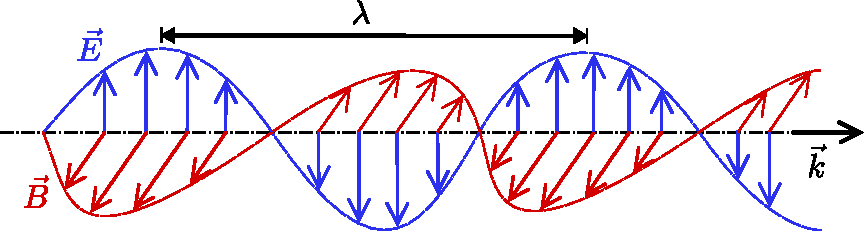
\psfig{file=fig/fig-onda-electromagnetica.pdf,height=3cm,angle=0}}
\caption{Campos el'ectrico y magn'etico de una onda electromagn'etica plana monocrom'atica. Adaptada a partir de \href{http://commons.wikimedia.org/wiki/File:Onde_electromagnetique.svg}{esta} figura original.}
\label{ondaem}
\end{figure}

\subsubsection{Vector de Poynting}
Evaluamos el vector de Poynting (\ref{defPoy}) para la soluci'on de onda plana monocrom'atica reci'en analizada. Usando (\ref{defPoy}), \eqref{BkE} y \eqref{rdoem} podemos escribir
\begin{eqnarray}
 \vec{S}&=&\vec{E}\times\vec{H} \\
&=&\frac{1}{\mu}\,\vec{E}\times\vec{B} \\
&=&\frac{1}{\mu}\,\vec{E}\times\left[\frac{1}{\omega}\,\vec{k}\times\vec{E}
\right] \\
&=&\frac{1}{\mu\omega}\,\vec{E}^2\,\vec{k}\\
&=&\frac{1}{\mu c}\,\vec{E}^2\,\hat{k}. \label{Sop}
\end{eqnarray}
Encontramos de este modo que el campo electromagn'etico correspondiente a la onda plana estudiada \textit{transporta energ'ia en la direcci'on del vector de onda $\vec{k}$}. Su magnitud, aunque siempre no-negativa, var'ia en el tiempo y con la posici'on, ya que $\vec{E}=\vec{E}(\vec{x},t)$. Como la onda considerada es peri'odica, de periodo $T=2\pi/\omega$, es usual considerar el \textbf{promedio del vector de Poynting en un periodo de oscilaci'on}\footnote{Si $f(t)$ es una funci'on del tiempo, entonces definimos su promedio entre $t=0$ y $t=T$ como 
\begin{equation}
\left<f\right>:=\frac{1}{T}\int_0^Tf(t)\,dt.
\end{equation}}
Para la onda sinusoidal (\ref{ecuc-max-solu1}) encontramos entonces que
\begin{equation}\label{Sprom}
\langle\vec{S}\rangle=\frac{1}{2\mu c}\,\vec{E}_0^2\,\hat{k}.
\end{equation}
Esto implica que a trav'es de una superficie de 'area $A$ transversal al vector de onda $\vec{k}$, la onda transporta energ'ia a una tasa (potencia) promedio (en una oscilaci'on) de 
\begin{equation}
 \left<P\right>=\frac{A}{2\mu c}\,\vec{E}_0^2.
\end{equation}

\subsubsection{Densidad de Energ'ia}
An'alogamente, calculamos la densidad de energ'ia electromagn'etica, usando la expresi'on (\ref{uDEHB}):
\begin{eqnarray}
 u&=&\frac{1}{2}\left(\varepsilon\vec{E}^2+\frac{1}{\mu}\vec{B}^2\right)\\
&=&\frac{1}{2}\left(\varepsilon\vec{E}^2+\frac{1}{\mu c^2}\vec{E}^2\right)\\
&=&\frac{1}{2}\left(\varepsilon\vec{E}^2+\varepsilon\vec{E}^2\right)\\
&=&\varepsilon\vec{E}^2. \label{uepE2}
\end{eqnarray}
Similarmente al caso del vector de Poynting, la densidad de energ'ia (siempre no-negativa) var'ia en el tiempo y punto a punto. 
Usando \eqref{uepE2} podemos reescribir el vector de Poynting (\ref{Sop}) como
\begin{equation}
 \vec{S}=u\,c\hat{k}.
\end{equation}
Note que esta expresi'on es an'aloga a $\vec{J}=\rho\vec{v}$ que relaciona la densidad de corriente asociada al movimiento de una densidad $\rho$ (de carga o masa, por ejemplo) con velocidad $\vec{v}$ (``flujo convectivo").

Para la onda peri'odica considerada, podemos calcular la densidad de energ'ia promedio, obteniendo
\begin{equation}\label{uprom}
\left<u\right>=\frac{\varepsilon}{2}\vec{E}_0^2.
\end{equation}

\begin{figure}[!h]
\centerline{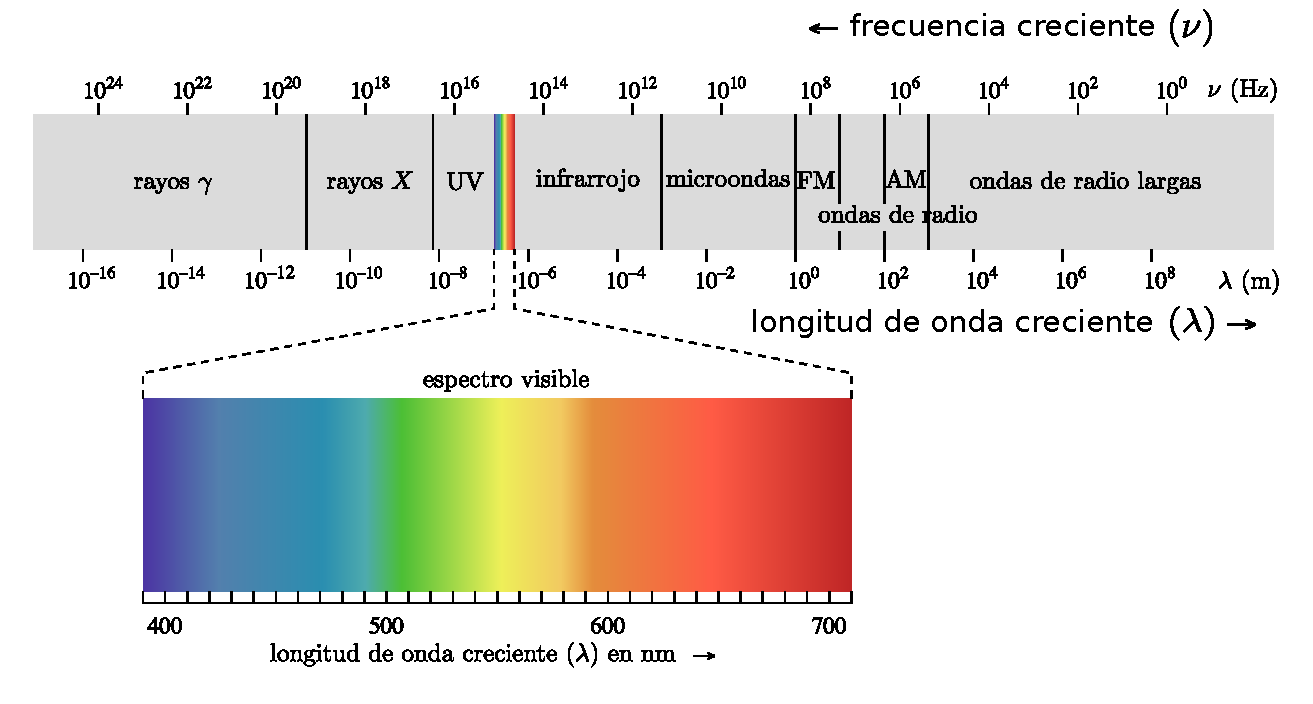
\psfig{file=fig/fig-EM_spectrum_es.pdf,height=7cm,angle=0}}
\caption{Espectro electromagn'etico. Adaptada a partir de \href{http://commons.wikimedia.org/wiki/File:EM_spectrum_es.svg}{esta} figura original.}
\label{fig:EMS}
\end{figure}

\subsection{Ondas electromagn'eticas en la materia}
\subsection{'Indices de reflexi'on y refracci'on}
\subsection{Gu'ias de onda y cavidades resonantes}


\section{Potenciales y transformaciones de gauge}

Las ecuaciones de Maxwell conforman un conjunto de 8 ecuaciones diferenciales
parciales para las 6 componentes del campo electromagn'etico. A menudo es
\textit{conveniente} reducir el n'umero de variables. Esto puede ser conseguido
expresando los campos en t'erminos de \textbf{potenciales electromagn'eticos},
de modo que \textit{las ecuaciones homog'eneas de Maxwell sean satisfechas
autom'aticamente} y el n'umero de campos a determinar se reduce a 4. Estos
potenciales se reducen en los casos estacionarios al conocido potencial
electrost'atico y al potencial vectorial magn'etico.

En el caso din'amico general, de (\ref{max2}) podemos concluir que $\vec{B}$
puede ser derivado de un \textbf{potencial vectorial}:
\begin{eqnarray}\label{defA2}
\boxed{\vec{B}=\vec{\nabla}\times \vec{A}.}
\end{eqnarray}
Usando esto en (\ref{max4}), obtenemos:
\begin{equation}
\vec{\nabla}\times \vec{E} = -  \frac{\partial\ }{\partial
t}(\vec{\nabla}\times\vec{A}) = -\vec{\nabla}\times
\frac{\partial\vec{A}}{\partial t},
\end{equation}
es decir,
\begin{eqnarray}
\vec{\nabla}\times \left[ \vec{E} + \frac{\partial \vec{A}}{\partial t} \right]
= \vec{0}.
\end{eqnarray}
De aqu'i vemos que el campo vectorial dado por la suma $\vec{E} + {\partial
\vec{A}}/{\partial t}$ puede ser escrito como gradiente de un campo escalar, esto es:
\begin{equation}
\vec{E} + \frac{\partial \vec{A}}{\partial t}= - \vec{\nabla}\phi ,
\end{equation}
de donde
\begin{equation}\label{defphi2}
\boxed{\vec{E} =   - \vec{\nabla}\phi - \frac{\partial \vec{A}}{\partial t}.}
\end{equation}
Las ecuaciones (\ref{defA2}) y (\ref{defphi2}) muestran que el campo
electromagn\'etico puede ser escrito en t\'erminos de un potencial vectorial
$\vec{A}$ y de un potencial escalar $\phi$. Sin embargo, estas funciones
\textit{no son 'unicas} para $\vec{E}$ y $\vec{B}$ dados. Es f\'acil verificar
que el campo electromagn\'etico (y consecuentemente todas las predicciones de la
teor'ia electromag\'etica) permanece invariante (es decir, con igual valor) bajo las
siguientes transformaciones de los potenciales,
\begin{equation}\marginnote{Transformaciones de gauge}\label{tgg}
\boxed{{\vec{A}}' = \vec{A} - \vec{\nabla}{\chi}, \qquad \phi' =\phi +
\frac{\partial \chi}{\partial t},}
\end{equation}
conocidas como \textbf{transformaciones de gauge} y donde $\chi=\chi(\vec{x},t)$
es una funci\'on escalar \textit{arbitraria} del espaciotiempo\footnote{La invariancia
de la teor'ia electromagn\'etica bajo transformaciones de gauge
desempe\~na un rol muy importante. La generalizaci\'on de esta propiedad de
invariancia a \textbf{grupos de simetr'ia interna} permiti\'o formular
teor'ias consistentes para las \textbf{interacciones d\'ebiles} unificadas con la electromagn\'etica (\textbf{electrod\'ebil}) y para la \textbf{interacci\'on fuerte}
(\textit{cromodin\'amica cu\'antica}). La \textbf{interacci'on gravitacional} tambi\'en puede ser descrita, con algunas peculiaridades, como una \textit{teor'ia de gauge}.}.

\subsubsection{Ecuaciones de Maxwell inhomog'eneas en t'erminos de los
potenciales}
Consideremos el caso de un medio lineal, is'otropo y homog'eneo. Usando (\ref{defA2}) y (\ref{defphi2}) en las ecuaciones inhomog'eneas (\ref{max1}) y (\ref{max3}) encontramos:
\begin{equation}\label{emiap1}
 \nabla^2\phi+\frac{\partial\ }{\partial t}\left(\vec{\nabla}\cdot\vec{A}\right)=-\frac{\rho}{\varepsilon},
\end{equation}
\begin{equation}\label{emiap2}
 \nabla^2\vec{A}-\frac{1}{c^2}\frac{\partial^2\vec{A}}{\partial t^2}-\vec{\nabla}\left(\vec{\nabla}\cdot\vec{A}+\frac{1}{c^2}\frac{\partial\phi }{\partial t}\right)=-\mu\,\vec{J}.
\end{equation}
De esta forma, hemos reducido las ecuaciones de Maxwell a un conjunto de 4 ecuaciones diferenciales parciales para los 4 potenciales. Sin embargo, estas ecuaciones no determinan completamente los potenciales, puesto que las transformaciones de gauge \eqref{tgg} \textit{dejan invariantes} \eqref{emiap1} y \eqref{emiap1}. Esto es natural ya que estas ecuaciones dependen en realidad de los campos el'ectrico y magn'etico, y como vimos las transformaciones de gauge no cambian los valores de estos campos. Adem'as, las ecuaciones \eqref{emiap1} y \eqref{emiap1} est'an \textit{acopladas}, en el sentido que cada una de estas ecuaciones involucra ambos potenciales electromagn'eticos.

Es posible explotar la ``\textbf{libertad de gauge}'' de la electrodin'amica (es decir, el hecho que los potenciales no son 'unicos) para \textit{simplificar algunos c'alculos}. Una forma de hacer esto es trabajar con potenciales que satisfagan alguna condici'on extra o \textbf{gauge}. De hecho, el imponer condiciones extras a los potenciales no s'olo es conveniente, sino tambi'en \textit{necesario}, ya que las ecuaciones \eqref{emiap1} y \eqref{emiap1} no determinan en forma 'unica los campos $\phi$ y $\vec{A}$. Es posible imponer infinitos gauges diferentes para los potenciales (siempre que sean consistentes con las ecuaciones de Maxwell), pero existen algunos de especial utilidad y popularidad.

\subsubsection{Gauge de Coulomb}
Si el potencial vectorial satisface
\begin{equation}\marginnote{Gauge de Coulomb}\label{gaugeC}
\boxed{ \vec{\nabla}\cdot\vec{A}\stackrel{!}{=}0,}
\end{equation}
se dice que se satisface el \textbf{gauge de Coulomb}, \textbf{gauge de radiaci'on} o \textbf{gauge transversal}. En este caso (\ref{emiap1}) y (\ref{emiap2}) se reducen a
\begin{equation}\label{emiap1GC}
 \nabla^2\phi=-\frac{\rho}{\varepsilon},
\end{equation}
\begin{equation}\label{emiap2GC}
 \nabla^2\vec{A}-\frac{1}{c^2}\frac{\partial^2\vec{A}}{\partial t^2}=-\mu\,\vec{J}+\frac{1}{c^2}\vec{\nabla}\left(\frac{\partial\phi }{\partial t}\right).
\end{equation}

Para probar que \textit{siempre es posible imponer la condici'on de gauge de Coulomb}, podemos considerar el caso en que inicialmente se trabaje con potenciales $\phi_0$ y $\vec{A}_0$ que no satisfacen la condici'on (\ref{gaugeC}), es decir, $\vec\nabla\cdot\vec{A}_0\neq 0$, y luego demostrar que es posible realizar una transformaci'on de gauge (\ref{tgg}) con una funci'on $\chi$ tal que los nuevos potenciales s'i satisfagan (\ref{gaugeC}). Usando (\ref{tgg}b) requerimos entonces que el nuevo potencial vectorial satisfaga
\begin{equation}
\vec\nabla\cdot\vec{A}=\vec\nabla\cdot(\vec{A}_0-\vec\nabla\chi)\stackrel{!}{=}0.
\end{equation}
Esto implica, como condici'on necesaria y suficiente, que la funci'on $\chi$ debe satisfacer 
\begin{equation}\label{ePchi}
\nabla^2\chi=\vec\nabla\cdot\vec{A}_0,
\end{equation}
es decir, la ecuaci'on de Poisson con una ``fuente'' conocida ($\vec\nabla\cdot\vec{A}_0$, dados los potenciales originales). Ya que han sido demostrados \textbf{teoremas de existencia} para esta ecuaci'on, es decir, que ella siempre tiene soluciones, queda demostrado que es \textit{posible} imponer el gauge de Coulomb. Note, sin embargo, que la funci'on $\chi$ que determina los nuevos potenciales que satisfacen el gauge de Coulomb \textit{no es 'unica}, ya que si $\chi_1$ es soluci'on de (\ref{ePchi}) entonces $\chi_2=\chi_1+\tilde\chi$ tambi'en es soluci'on, siempre que $\tilde\chi$ sea una soluci'on de la ecuaci'on de Laplace ($\nabla^2\tilde\chi=0$). Existe entonces una ``\textbf{libertad remanente}'' para seguir realizando transformaciones de gauge, generadas por funciones $\tilde\chi$ que satisfacen la ecuaci'on de Laplace, y que permiten imponer algunas condiciones\footnote{Ojo: no \textit{cualquier} condici'on, sino aquellas que sean compatibles con el resto de las condiciones, y con las ecuaciones de Maxwell.} adicionales a los potenciales, siempre dentro de la ``familia de potenciales'' que satisface el gauge de Coulomb.

Una de las conveniencias de este gauge es que \textit{la ecuaci'on (\ref{emiap1GC}) tiene la misma forma que en el caso electrost'atico}\footnote{Se dice por esto que es ``\textit{coulombiano}'', de ah'i uno de los nombres asociados a este gauge.}. Debido a esto, y usando la ``libertad remanente'' mencionada anteriormente, es posible elegir\footnote{!`Pruebe esta afirmaci'on!.} el potencial escalar de la forma siguiente:
\begin{equation}\label{phiGC}
\boxed{ \phi(\vec{x},t)=\frac{1}{4\pi\varepsilon}\int\frac{\rho(\vec{x}',t)}{\left|\vec{x}-\vec{x}'\right|}dV'.}
\end{equation}
Esta soluci'on para el potencial puede entonces ser reemplazada en el lado derecho de \eqref{emiap2GC}. 
%Sin embargo, un c'alculo sencillo muestra que este 'ultimo t'ermino cancela la \textit{componente irrotacional} (``longitudinal'') de la corriente. En efecto, asumiendo que las fuentes son localizadas, podemos usar el resultado descrito en el ap'endice \ref{Apcamps} y separar la densidad de corriente en una componente longitudinal,  $\vec{J}_{\rm l}$, (o irrotacional, con $\vec\nabla\times\vec{J}_{\rm l}=0$) y una transversal,  $\vec{J}_{\rm t}$, (o solenoidal, con $\vec\nabla\cdot\vec{J}_{\rm t}=0$):
%\begin{equation}
% \vec{J}=\vec{J}_{\rm l}+\vec{J}_{\rm t},
%\end{equation}
%con
%\begin{equation}
% \vec{J}_{\rm l} =-\frac{1}{4\pi}\vec\nabla\int\frac{(\vec\nabla\cdot\vec{J})(\vec{x}')}{|\vec{x}-\vec{x}'|}dV',
%\end{equation}
%\begin{equation}
% \vec{J}_{\rm t} =\frac{1}{4\pi}\vec\nabla\times\int\frac{(\vec\nabla\times\vec{J})(\vec{x}')}{|\vec{x}-\vec{x}'|}dV'.
%\end{equation}
A partir de (\ref{phiGC}), y usando la ecuaci'on de continuidad, podemos escribir el segundo t'ermino del lado derecho de \eqref{emiap2GC} s'olo en t'erminos de la densidad de corriente, ya que
\begin{eqnarray}
\vec{\nabla}\left(\frac{\partial\phi }{\partial t}\right)&=&  \vec{\nabla}\frac{\partial\ }{\partial t}\left(\frac{1}{4\pi\varepsilon}\int\frac{\rho(\vec{x}',t)}{\left|\vec{x}-\vec{x}'\right|}dV'\right) \\
&=&  \frac{1}{4\pi\varepsilon}\vec{\nabla}\int\frac{\frac{\partial\rho }{\partial t}(\vec{x}',t)}{\left|\vec{x}-\vec{x}'\right|}dV' \\
&=& - \frac{1}{4\pi\varepsilon} \vec{\nabla}\int\frac{(\vec{\nabla}'\cdot\vec{J}')}{\left|\vec{x}-\vec{x}'\right|}dV' .%\\
%&=& \frac{1}{\varepsilon}\vec{J}_{\rm l}.
\end{eqnarray}
Con esto, la ecuaci'on (\ref{emiap2GC}) se reduce a
\begin{equation}\label{emiap3GC}
\boxed{\nabla^2\vec{A}-\frac{1}{c^2}\frac{\partial^2\vec{A}}{\partial t^2}=-\mu\,\vec{J}_{\rm T},}
\end{equation}
donde hemos introducido la \textbf{componente transversal de la densidad de corriente}
\begin{align}
\vec{J}_{\rm T} &:= \vec{J}-\frac{1}{c^2\mu}\vec{\nabla}\left(\frac{\partial\phi }{\partial t}\right) \\
&= \vec{J}+\frac{1}{4\pi} \vec{\nabla}\int\frac{(\vec{\nabla}'\cdot\vec{J}')}{\left|\vec{x}-\vec{x}'\right|}dV'.
\end{align}
Se dice que este campo es \textit{transversal} porque satisface
\begin{equation}
\vec\nabla\cdot\vec{J}_{\rm T}\equiv 0.
\end{equation}

En resumen, \textit{en el gauge de Coulomb el potencial vectorial satisface la  \textit{ecuaci'on de onda inhomog'enea}, con un t'ermino fuente determinado s'olo por la componente transversal de la densidad de corriente}. Adem'as, en este gauge  s'olo el potencial vectorial contribuye a los \textbf{campos radiativos}\footnote{Como veremos en el cap'itulo \ref{caprad}, se dice que un campo electromagn'etico es radiativo si su contribuci'on a la energ'ia radiada muy lejos de las fuentes (``en el infinito'') es no nula.}. En cambio, el potencial escalar \eqref{phiGC} es no-radiativo como consecuencia de que su valor decae al menos tan r'apido como $1/r$ a grandes distancias de la fuente.

El gauge de Coulomb es a menudo usado en regiones donde no hay fuentes presentes. En este caso es posible elegir $\phi=0$, ver \eqref{phiGC}, de modo que toda la informaci'on del campo electromagn'etico est'a contenida en el potencial vectorial $\vec{A}$.


\subsubsection{Gauge de Lorenz}
Otro gauge com'un es el \textbf{gauge de Lorenz}\footnote{Nombrado en recuerdo de Ludvig Valentin Lorenz (1829-1891): Matem'atico y F'isico Dan'es. Ver \url{http://es.wikipedia.org/wiki/Ludvig_Lorenz}, quien consider'o esta elecci'on en 1867.}, que usualmente es escrito como
\begin{equation}\marginnote{Gauge de Lorenz}\label{gLorenz}
\boxed{\frac{1}{c^2}\frac{\partial\phi}{\partial t}+\vec{\nabla}\cdot\vec{A}\stackrel{!}{=}0,}
\end{equation}
y que \textit{permite desacoplar las ecuaciones} (\ref{emiap1}) y (\ref{emiap2}).
En efecto, si (\ref{gLorenz}) es satisfecha entonces (\ref{emiap1}) y (\ref{emiap2}) se reducen a
\begin{equation}\label{emiap1gL}
 \nabla^2\phi-\frac{1}{c^2}\frac{\partial^2\phi}{\partial t^2}=-\frac{\rho}{\varepsilon},
\end{equation}
\begin{equation}\label{emiap2gL}
 \nabla^2\vec{A}-\frac{1}{c^2}\frac{\partial^2\vec{A}}{\partial t^2}=-\mu\,\vec{J},
\end{equation}
o, introduciendo el \textbf{operador de onda} (u operador de  d'\,Alembert\footnote{Jean Le Rond d'\,Alembert (1717-1783): matem'atico, fil'osofo y enciclopedista franc'es. Ver \url{http://es.wikipedia.org/wiki/Jean_le_Rond_d\%27Alembert}.}), 
$\Box:= c^{-2}{\partial^2}/{\partial t^2}-\nabla^2$,
\begin{equation}\label{emiap1gL2}
 \Box\phi=\frac{\rho}{\varepsilon},
\end{equation}
\begin{equation}\label{emiap2gL2}
 \Box\vec{A}=\mu\,\vec{J}.
\end{equation}

An'alogamente al caso del gauge de Coulomb, puede probarse que \textit{el gauge de Lorenz siempre puede ser impuesto}, considerando que inicialmente se usen potenciales ($\phi_0$ y $\vec{A}_0$) que no lo satisfacen, y mostrando que puede encontrarse una funci'on $\chi$ que genere la transformaci'on de gauge apropiada para que los nuevos potenciales s'i la satisfagan. En este caso, la condici'on sobre la funci'on $\chi$ requerida es que
\begin{eqnarray}
0&\stackrel{!}{=}&\frac{1}{c^2}\frac{\partial\phi}{\partial t}+\vec{\nabla}\cdot\vec{A} \\
&=&\frac{1}{c^2}\frac{\partial\ }{\partial t}\left(\phi_0+\frac{\partial\chi}{\partial t}\right)+\vec{\nabla}\cdot\left(\vec{A}_0-\vec\nabla\chi\right) \\
&=&\left(\frac{1}{c^2}\frac{\partial\phi_0}{\partial t} +\vec{\nabla}\cdot\vec{A}_0\right) +\frac{1}{c^2}\frac{\partial^2\chi }{\partial t^2}-\nabla^2\chi,
\end{eqnarray}
es decir, que satisfaga la ecuaci'on de onda inhomog'enea:
\begin{equation}
\Box\chi=-\left(\frac{1}{c^2}\frac{\partial\phi_0}{\partial t} +\vec{\nabla}\cdot\vec{A}_0\right).
\end{equation}
La existencia de soluciones de esta ecuaci'on est'a garantizada. An'alogamente al caso del gauge de Coulomb, la funci'on buscada no es 'unica, sino que existe una libertad remanente para realizar transformaciones de gauge ``dentro del gauge de Lorenz'', generadas por funciones $\tilde\chi$ que satisfagan la ecuaci'on de onda, $\Box\tilde\chi=0$. 

El gauge de Lorenz es usado com'unmente en el contexto de la teor'ia de Especial de la Relatividad, ya que en el vac'io (cuando $\varepsilon=\varepsilon_0$ y $\mu=\mu_0$ y por lo tanto $c=c_0$) la condici'on (\ref{gLorenz}) as'i como (\ref{emiap1gL2}) y (\ref{emiap2gL2}), \textit{mantienen su forma inalterada en cualquier sistema de referencia inercial} (son \textit{covariantes} bajo transformaciones de Lorentz). Esto tiene como consecuencia que toda expresi'on que involucre a los potenciales electromag'eticos (que satisfagan el gauge de Lorenz) tendr'a la \textit{misma forma en todo Sistema de Referencia Inercial}. Esto no ocurre, por ejemplo, si se usan potenciales que satisfagan el gauge de Coulomb.
\newpage
\chapter{Teor'ia Cl'asica de la Radiaci'on Electromagn'etica}\label{caprad}

\section{Resolviendo las ecuaciones de Maxwell.}\label{resolvmax}

Las ecuaciones de Maxwell inhomog'eneas, escritas en t'erminos de los potenciales electromagn'eticos y en el gauge de Lorenz, se reducen a
%\begin{equation}
%\boxed{\Box A^\mu   =\frac{4\pi}{c}J^\mu ,}
%\end{equation}
%o, equivalentemente,
%\begin{equation}
%\Box \phi   =4\pi \rho, \qquad \Box \vec{A}=\frac{4\pi}{c}\vec{J}.
%\end{equation}
\begin{equation}
 \Box\phi=\frac{\rho}{\varepsilon}, \qquad  \Box\vec{A}=\mu\,\vec{J}.
\end{equation}
Estas son las ecuaciones que resolveremos: las ecuaciones de onda
inhomog'eneas para fuentes dadas. Todas ellas son de la forma
\begin{equation}
\Box \Psi(\vec{x},t)=g(\vec{x},t), \label{oih}
\end{equation}
con una funci'on ``fuente'' $g(\vec{x},t)$ dada.


\subsection{Ecuaci'on de Helmholtz inhomog'enea y funci'on de Green independiente del tiempo}
\subsubsection{Transformada de Fourier}
Primero introduciremos la \textbf{transformada de Fourier temporal} de los campos involucrados (suponemos que estos campos son cuadrado-integrables),
\begin{equation}
\bar{\Psi}(\vec{x},\omega):=\frac{1}{\sqrt{2\pi}}\int_{-\infty}^\infty
\Psi(\vec{x},t)e^{-i\omega t}\,dt,
\end{equation}
\begin{equation}
\bar{g}(\vec{x},\omega):=\frac{1}{\sqrt{2\pi}}\int_{-\infty}^\infty
g(\vec{x},t)e^{-i\omega t}\,dt ,
\end{equation}
y entonces
\begin{equation}
g(\vec{x},t)=\frac{1}{\sqrt{2\pi}}\int_{-\infty}^\infty
\bar{g}(\vec{x},\omega)e^{+i\omega t}\,d\omega,
\end{equation}
\begin{equation}
\Psi(\vec{x},t)=\frac{1}{\sqrt{2\pi}}\int_{-\infty}^\infty
\bar{\Psi}(\vec{x},\omega)e^{+i\omega t}\,d\omega.
\end{equation}

Usando estas transformaciones la ecuaci'on (\ref{oih}) se reduce a la ecuaci'on de
Helmholtz inhomog'enea:
\begin{equation}
\left[ \nabla^2+k^2\right] \bar{\Psi}(\vec{x},\omega)=-\bar{g}(\vec{x},\omega),
\label{Hih}
\end{equation}
con $k:=\omega/c$. Resolveremos esta ecuaci'on \textit{independiente del tiempo} por medio del m'etodo de la funci'on de Green.

\subsubsection{Funci'on de Green independiente del tiempo}
La funci'on de Green asociada a nuestro problema es
\begin{equation}
\left[ \nabla^2+k^2\right] G(\vec{x},\vec{x}')=+\delta^{(3)}(\vec{x}-\vec{x}').
\label{ecGreen}
\end{equation}
Si logramos resolver (\ref{ecGreen}) y encontrar una soluci'on $G(\vec{x},\vec{x}')$ entonces una soluci'on particular de (\ref{Hih}) es de la forma
\begin{equation}
\bar{\Psi}(\vec{x},\omega)=-\int G(\vec{x},\vec{x}')\bar{g}(\vec{x}',\omega)\,dV'.
\end{equation}
La funci'on de Green $G(\vec{x},\vec{x}')$ puede considerarse como un caso particular de soluci'on de (\ref{Hih}) correspondiente a una funci'on fuente $\bar{g}=\delta^{(3)}(\vec{x}-\vec{x}')$. En t'erminos m'as f'isicos, la funci'on de Green $G(\vec{x},\vec{x}')$ es proporcional al campo producido por una \textbf{fuente puntual}. En efecto, si $g(\vec{x},t)=f(t)\delta^{(3)}(\vec{x}-\vec{x}')$, entonces $\bar{g}(\vec{x},\omega)=\bar{f}(\omega)\delta^{(3)}(\vec{x}-\vec{x}')$, donde $\bar{f}(\omega)$ es la transformada de Fourier de $f(t)$. De lo anterior, vemos que en este caso la soluci'on de (\ref{Hih}) es de la forma $-\bar{f}(\omega)G(\vec{x},\vec{x}')$.

La funci'on de Green que satisface (\ref{ecGreen}) \textit{no es 'unica}, siempre es posible sumar una soluci'on de la ecuaci'on de Helmholtz homog'enea. De entre las posibles soluciones, encontraremos aquella que satisfaga \textit{condiciones de simetr'ia apropiadas a nuestro problema}. En particular, deseamos encontrar las soluciones particulares que describan los campos \textit{generados por una distribuci'on de cargas y corrientes dada}, sin incluir los campos generados por \textit{fuentes externas al sistema} (y que satisfacen la ecuaci'on homog'enea en el dominio bajo consideraci'on).

Ya que $G(\vec{x},\vec{x}')$ determina la dependencia espacial de la soluci'on correspondiente a una carga puntual situada en $\vec{x}'$, esperamos que 'esta sea esf'ericamente sim'etrica en torno a este punto (``isotrop'ia del espacio''), y s'olo dependiente de la diferencia entre $\vec{x}$ y $\vec{x}'$ (``homogeneidad del espacio''). Entonces, supondremos que $G$ depende de $\vec{x}$ y $\vec{x}'$ s'olo a trav'es de la combinaci'on $|\vec{x}-\vec{x}'|$. Si
\begin{equation}
G(\vec{x},\vec{x}')=G(|\vec{x}-\vec{x}'|),
\end{equation}
 la ecuaci'on (\ref{ecGreen}) se reduce a
\begin{equation}
\left[ \nabla^2+k^2\right] G(r)=\delta^{(3)}(r), \qquad r:=|\vec{r}|.
\end{equation}
%ya que, sin perder generalidad, es posible elegir $\vec{x}'=\vec{0}$.
En coordenadas esf'ericas, tendremos entonces que
\begin{equation}
 \frac{1}{r^2}\frac{d}{dr}\left( r^2\frac{dG}{dr}\right) +k^2G(r)=\delta^{(3)}(r)
.\label{HelmG}
\end{equation}
Es directo resolver (\ref{HelmG}) para puntos $r\neq 0$. Obtenemos:
\begin{equation}
G(r)=\alpha\frac{e^{\pm ikr}}{r}, \label{G0}
\end{equation}
para $r\neq 0$. La constante $\alpha$ debe ser determinada de modo que
(\ref{G0}) sea v'alida para todo punto, incluyendo el punto $r=0$. Usando
$\vec{\nabla}r=-r^2\vec{\nabla}\left({1}/{r}\right) $, podemos escribir:
\begin{eqnarray}
\vec{\nabla}G&=&\pm ik\alpha\frac{1}{r}\left( \vec{\nabla}r\right) e^{\pm
ikr}+\alpha e^{\pm ikr} \vec{\nabla}\left( \frac{1}{r}\right) \\
&=&\mp ik\alpha r\vec{\nabla}\left( \frac{1}{r}\right)  e^{\pm ikr}+\alpha
e^{\pm ikr} \vec{\nabla}\left( \frac{1}{r}\right) .
\end{eqnarray}
Similarmente,
\begin{eqnarray}
\nabla^2G&=&\vec{\nabla}\cdot \vec{\nabla}G \\
&=&\mp ik\alpha r\left( \vec{\nabla}r\right)\cdot\vec{\nabla}\left(
\frac{1}{r}\right)  e^{\pm ikr}\mp ik\alpha r \nabla^2\left( \frac{1}{r}\right)
e^{\pm ikr}+k^2\alpha r\left( \vec{\nabla}r\right)\cdot\vec{\nabla}\left(
\frac{1}{r}\right)  e^{\pm ikr}\nonumber\\
&&\pm ik\alpha e^{\pm ikr} \left( \vec{\nabla}r\right)\cdot\vec{\nabla}\left(
\frac{1}{r}\right) +\alpha e^{\pm ikr}\nabla^2\left( \frac{1}{r}\right) \\
&=&\mp ik\alpha r \nabla^2\left( \frac{1}{r}\right)  e^{\pm ikr}+k^2\alpha
r\left( \vec{\nabla}r\right)\cdot\vec{\nabla}\left( \frac{1}{r}\right)  e^{\pm
ikr}+\alpha e^{\pm ikr}\nabla^2\left( \frac{1}{r}\right) \\
&=&\mp ik\alpha r \nabla^2\left( \frac{1}{r}\right)  e^{\pm ikr}-k^2\alpha
\frac{1}{r} \left|\vec{\nabla}r\right|^2  e^{\pm ikr}+\alpha e^{\pm
ikr}\nabla^2\left( \frac{1}{r}\right).
\end{eqnarray}
Usando ahora $\nabla^2\left({1}/{r}\right) =-4\pi\delta^{(3)}(r)$,
$f(r)\delta^{(3)}(r)=f(0)\delta^{(3)}(r)$ para una funci'on $f(r)$ arbitraria, y
$\vec{\nabla}r=\hat{r}$, de modo que $|\vec{\nabla}r|=1$,
encontramos
\begin{eqnarray}
\nabla^2G&=&\pm 4\pi ik\alpha r  e^{\pm ikr}\delta^{(3)}(r) -k^2\alpha \frac{1}{r}
e^{\pm ikr}-4\pi\alpha e^{\pm ikr}\delta^{(3)}(r) \\
&=&0-k^2\alpha \frac{e^{\pm ikr}}{r}   -4\pi\alpha \delta^{(3)}(r) \\
&=&-k^2G(r) -4\pi\alpha \delta^{(3)}(r) .\label{lapG}
\end{eqnarray}
Comparando (\ref{lapG}) con (\ref{HelmG}) obtenemos $\alpha=-{1}/{4\pi}$, de
modo que la funci'on de Green para nuestro problema es
\begin{equation}
\boxed{G(\vec{x},\vec{x}')=-\frac{1}{4\pi}\frac{e^{\pm
ik|\vec{x}-\vec{x}'|}}{|\vec{x}-\vec{x}'|}, \qquad k:=\frac{\omega}{c}.} \label{Green}
\end{equation}


\subsection{Potenciales retardados}
Con la funci'on de Green (\ref{Green}) obtenemos la soluci'on particular para la
transformada de Fourier $\bar{\Psi}(\vec{x},\omega)$:
\begin{equation}
\bar{\Psi}(\vec{x},\omega)=\frac{1}{4\pi}\int
\bar{g}(\vec{x}',\omega)\frac{e^{\pm
ik|\vec{x}-\vec{x}'|}}{|\vec{x}-\vec{x}'|}\,dV' .
\end{equation}
Con esto, podemos finalmente calcular la soluci'on particular de la ecuaci'on de
onda inhomog'enea (\ref{oih}):
\begin{eqnarray}
\Psi(\vec{x},t)&=&\frac{1}{\sqrt{2\pi}}\frac{1}{4\pi}\int_{V'}\int_{-\infty}
^\infty \bar{g}(\vec{x}',\omega)\frac{e^{\pm
ik|\vec{x}-\vec{x}'|}}{|\vec{x}-\vec{x}'|}e^{i\omega t}\,d\omega\,dV'  \\
&=&\frac{1}{\sqrt{2\pi}}\frac{1}{4\pi}\int_{V'}\frac{1}{|\vec{x}-\vec{x}'|}\int_
{-\infty}^\infty \bar{g}(\vec{x}',\omega)e^{i\omega t_{\pm}}\,d\omega \,dV' \\
&=&\frac{1}{4\pi}\int_{V'} \frac{g(\vec{x}',t_{\pm})}{|\vec{x}-\vec{x}'|}\,dV' .
\end{eqnarray}
En la expresi'on anterior hemos denotado
\begin{equation}
t_{\pm}:=t\pm \frac{|\vec{x}-\vec{x}'|}{c}.
\end{equation}
Los \textbf{potenciales retardados} corresponden a la soluci'on con
\begin{equation}
\boxed{t_{\rm ret}:=t-\frac{|\vec{x}-\vec{x}'|}{c},} \label{deftret}
\end{equation}
que es llamado el \textbf{tiempo retardado} (puesto que $t_{\rm ret}\le t$), de modo que
\begin{equation}
\boxed{\phi_{\rm ret}(\vec{x},t)=\frac{1}{4\pi\varepsilon}\int_{V'}
\frac{\rho(\vec{x}',t_{\rm ret})}{|\vec{x}-\vec{x}'|}\,dV',} \qquad \boxed{\vec{A}_{\rm
ret}(\vec{x},t)=\frac{\mu}{4\pi}\int_{V'}
\frac{\vec{J}(\vec{x}',t_{\rm ret})}{|\vec{x}-\vec{x}'|}\,dV' ,} \label{potret}
\end{equation}
suministran expresiones para los potenciales electromagn'eticos en un punto
$\vec{x}$ y en un instante $t$ dado \textit{en t'erminos de la distribuci'on de cargas y corrientes en tiempos anteriores a} $t$ (``soluci'on causal''). En otras palabras, los potenciales (\ref{potret}) permiten \textit{pre}decir los campos producidos por un sistema de cargas dado. La soluci'on correspondiente al \textbf{tiempo avanzado} $t_{\rm av}:=t+{|\vec{x}-\vec{x}'|}/{c}\ge t$ no ser'a usada puesto que conduce, en cada instante $t$, a campos determinados por la distribuci'on de cargas en \textit{tiempos posteriores a }$t$ (``soluci'on acausal'').

Las expresiones para los potenciales retardados son similares a aquellas v'alidas los casos electrost'atico y magnetost'atico, ver \eqref{perho} y \eqref{defA} respectivamente, salvo que las fuentes dentro de la integral est'an evaluadas en el tiempo retardado, que depende tanto del tiempo como de la posici'on\footnote{Esta propiedad no es en general v'alida si los potenciales satisfacen gauges distintos al de Lorenz.}. Esta soluci'on muestra que los campos en un punto $\vec{x}$ y tiempo $t$ dado son una  \textit{superposici'on de t'erminos proporcionales a las fuentes ubicadas en \textit{cada punto} $\vec{x}'$, pero en tiempos anteriores} $t_{\rm ret}$, de forma tal que el \textit{evento}\footnote{es decir, un punto determinado del espacio y del tiempo.} definido por $(ct_{\rm ret},\vec{x}')$ tiene una \textit{relaci'on tipo luz} con el evento $(ct,\vec{x})$. Esto 'ultimo significa, como se desprende de (\ref{deftret}), que
\begin{equation}\marginnote{relaci'on tipo luz}
 c^2(t-t_{\rm ret})^2-|\vec{x}-\vec{x}'|^2=0.
\end{equation}
En otras palabras, los valores del campo en un evento dado est'an determinados por los valores de las fuentes en los puntos del \textbf{cono de luz pasado} asociado a tal evento. Ver figura \ref{fig:cdl2}.
\begin{figure}[!h]
\centerline{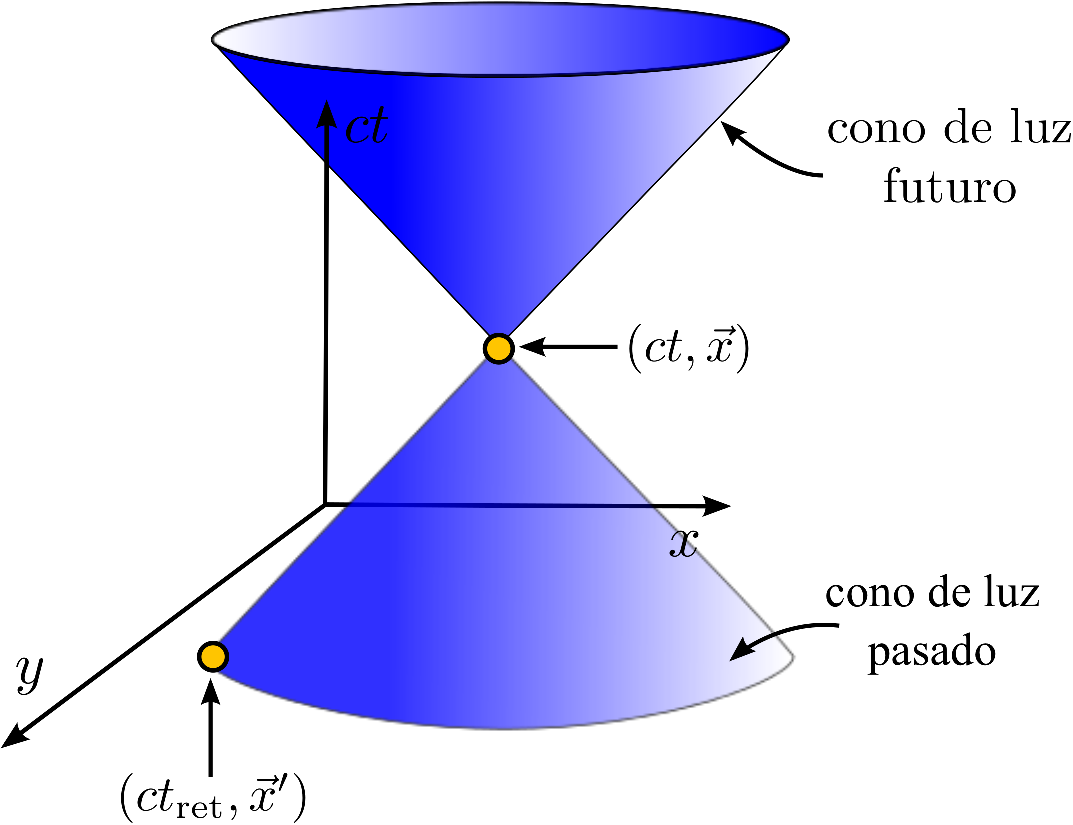
\includegraphics[height=5.5cm]{fig/fig-cono-de-luz-01.pdf}}
\caption{Cono de luz}
\label{fig:cdl2}
\end{figure}

Otra consecuencia directa es que cualquier \textit{cambio} en la configuraci'on de las fuentes en un punto afectar'a a los campos en otro punto s'olo en tiempos posteriores, luego de un intervalo de tiempo igual al tiempo de vuelo de una se\~nal luminosa que los conecte. En otras palabras: \textit{los cambios de los campos producidos por cambios de las fuentes se propagan con rapidez $c=1/\sqrt{\varepsilon\mu}$}. Equivalentemente, el valor de las fuentes en un determinado evento contribuye a los valores de los campos s'olo en eventos situados sobre el \textit{cono de luz futuro} del evento fuente.

\section{Ecuaciones de Jefimenko}
A partir de las expresiones para los potenciales retardados en el gauge de Lorenz, es decir las ecuaciones \eqref{potret}, podemos calcular los campos el'ectrico y magn'etico producidos por una distribuci'on (arbitraria, pero compacta) de cargas y corrientes:
\begin{equation}
\vec{E}(\vec{x},t)=\frac{1}{4\pi\varepsilon}\int_V \left[  \frac{\rho(\vec{x}',t_{\rm ret})(\vec{x}-\vec{x}')}{\vert \vec{x}-\vec{x}' \vert^3} + \frac{1}{c}\frac{ \dot\rho(\vec{x}',t_{\rm ret})(\vec{x}-\vec{x}')}{\vert\vec{x}-\vec{x}'\vert^2} -\frac{1}{c^2}\frac{\dot{\vec{J}} (\vec{x}',t_{\rm ret})}{\vert\vec{x}-\vec{x}' \vert} \right] dV',
\end{equation}
\begin{equation}
\vec{B}(\vec{x},t)=\frac{\mu}{4\pi} \int_V\left[
\frac{\vec{J}(\vec{x}',t_{\rm ret})\times(\vec{x}-\vec{x}')}{\vert \vec{x}-\vec{x}'\vert^3}+ \frac{1}{c}\frac{ \dot{\vec{J}}(\vec{x}',t_{\rm ret})\times(\vec{x}-\vec{x}')}{\vert\vec{x}-\vec{x}' \vert^2} \right]dV', \label{b3}
\end{equation}
donde $\dot{f}(\vec{x},t)$ denota la derivada partial respecto a la variable temporal de la que depende la funci'on $f(\vec{x},t)$, es decir $\dot{f}(\vec{x},t):=(\partial_t f)(\vec{x},t)$. Las relaciones anteriores son conocidas como \textbf{ecuaciones de Jefimenko}\footnote{\href{http://en.wikipedia.org/wiki/Jefimenko}{Oleg Jefimenko} (1922-2009): f'isico estadounidense.}. Note que estas expresiones para los campos el'ectrico y magn'etico difieren de aquellas que se encontrar'ian directamente la soluci'on de las ecuaciones inhomog'eneas \eqref{EcOihE} y \eqref{EcOihB}. ?`Puede explicar por qu'e ocurre esto?.


\section{Potenciales de Li'enard-Wiechert}

Se conoce como \textbf{potenciales de Li'enard}\footnote{\href{https://en.wikipedia.org/wiki/Alfred-Marie_Li\%C3\%A9nard}{Alfred Marie Li\'enard} (1869-1958): f'isico franc'es.}\textbf{-Wiechert}\footnote{\href{https://en.wikipedia.org/wiki/Emil_Wiechert}{Johann Emil Wiechert} (1861-1928): (geo)f'isico alem'an.} a los potenciales retardados generados por una \textit{carga puntual} $q$ \textit{que se mueve en forma conocida, pero arbitraria, con trayectoria} $\vec{z}(t)$. Ver figura (\ref{fig:LW}).
\begin{figure}[ht]
\centerline{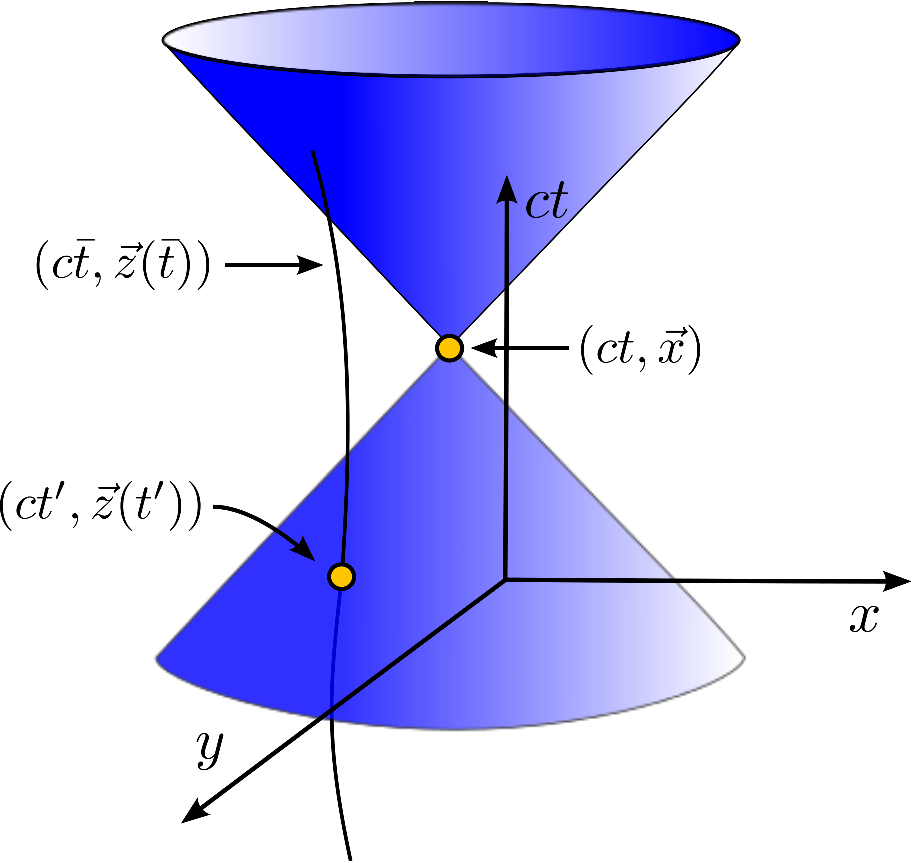
\includegraphics[height=5.5cm]{fig/fig-cono-de-luz-02.pdf}}
\caption{Trayectoria de una carga puntual y cono de luz asociado al evento $(ct,\vec{x})$.}
\label{fig:LW}
\end{figure}
En este caso, la densidad de carga y de corriente est'an dadas por
\begin{equation}
\rho(\vec{x},t)=q\delta^{(3)}(\vec{x}-\vec{z}(t)), \qquad
\vec{J}(\vec{x},t)=q\vec{v}(t)\delta^{(3)}(\vec{x}-\vec{z}(t)),
\end{equation}
donde $\vec{v}(t)={d\vec{z}}/{dt}$. Por lo tanto, los potenciales retardados (\ref{potret}) se reducen a
\begin{equation}
\phi_{\rm ret}(\vec{x},t)=\frac{q}{4\pi\varepsilon}\int_{V'}
\frac{\delta^{(3)}(\vec{x}'-\vec{z}(t_{\rm ret}))}{|\vec{x}-\vec{x}'|}\,dV', \qquad
\vec{A}_{\rm ret}(\vec{x},t)=\frac{q\mu}{4\pi}\int_{V'}
\frac{\vec{v}(t_{\rm ret})\delta^{(3)}(\vec{x}'-\vec{z}(t_{\rm ret}))}{|\vec{x}-\vec{x}'|}\,dV'  \label{potretq1}
\end{equation}
o, m'as expl'icitamente,
\begin{equation}
\phi_{\rm ret}(\vec{x},t)=\frac{q}{4\pi\varepsilon}\int_{V'}
\frac{\delta^{(3)}(\vec{x}'-\vec{z}(t-|\vec{x}-\vec{x}'|/c))}{|\vec{x}-\vec{x}'|}\,dV', \end{equation}
\begin{equation}
\vec{A}_{\rm ret}(\vec{x},t)=\frac{q\mu}{4\pi}\int_{V'}
\frac{\vec{v}(t-|\vec{x}-\vec{x}'|/c)\,\delta^{(3)}(\vec{x}'-\vec{z}(t-|\vec{x}-\vec{x}'|/c))}{|\vec{x}-\vec{x}'|}\,dV' . \label{potretq2}
\end{equation}
Ambas expresiones son de la forma
\begin{equation}
I(\vec{x},t)=\int_{V'}
f(\vec{x},\vec{x}',t)\,\delta^{(3)}(\vec{x}'-\vec{z}(t-|\vec{x}-\vec{x}'|/c))\,d^3x' . \label{potretqg1}
\end{equation}

Para calcular este tipo de integrales, expresaremos la delta de Dirac 3-dimensional como una integral sobre la variable (temporal) auxiliar $T$:
\begin{equation}
 \delta^{(3)}(\vec{x}'-\vec{z}(t-|\vec{x}-\vec{x}'|/c))=\int_T \delta^{(3)}(\vec{x}'-\vec{z}(T))\,\delta(T-t+|\vec{x}-\vec{x}'|/c)\, dT.
\end{equation}
Con esto,
\begin{equation}
I(\vec{x},t)=\int_{T}\int_{V'}
f(\vec{x},\vec{x}',t)\,\delta^{(3)}(\vec{x}'-\vec{z}(T))\,\delta(T-t+|\vec{x}-\vec{x}'|/c)\,d^3x' \, dT. \label{potretqgm11}
\end{equation}
Expresada de esta forma, es sencillo realizar la integral espacial, puesto que la delta de Dirac 3-dimensional evaluar'a la coordenada $\vec{x}'$ en el punto $\vec{z}(T)$, es decir, en un punto sobre la trayectoria de la carga. As'i, obtenemos
\begin{equation}
I(\vec{x},t)=\int_{T}f(\vec{x},\vec{z}(T),t)\,\delta(T-t+|\vec{x}-\vec{z}(T)|/c)\, dT. \label{potretqgm12}
\end{equation}
El argumento de la delta de Dirac es una funci'on no trivial $g$ de la variable auxiliar $T$. Denotamos
\begin{equation}
 g(T):=T-t+\frac{1}{c}|\vec{x}-\vec{z}(T)|,
\end{equation}
de modo que
\begin{eqnarray}
I(\vec{x},t)&=&\int_{T}f(\vec{x},\vec{z}(T),t)\,\delta(g(T))\, dT \\
&=&\int_{T}f(\vec{x},\vec{z}(T),t)\frac{\delta(T-t')}{|g'(t')|}\, dT \\
&=&\frac{f(\vec{x},\vec{z}(t'),t)}{|g'(t')|}, \label{Ir}
\end{eqnarray}
donde $g'$ es la funci'on derivada de $g$ y $t'$ es la soluci'on de la ecuaci'on $g(t')=0$, es decir, de
\begin{equation}
 t'=t-\frac{1}{c}|\vec{x}-\vec{z}(t')|. \label{t'}
\end{equation}
Esta relaci'on define una ecuaci'on algebraica para $t'$ cuya soluci'on define, \textit{conocida la trayectoria de la carga}, un tiempo retardado $t'=t'(\vec{x},t)$. Adem'as, usando la regla de la cadena, encontramos
\begin{equation}
 g'(t')=1-\frac{1}{c}\frac{\vec{v}(t')\cdot\left(\vec{x}-\vec{z}'(t')\right)}{\left|\vec{x}-\vec{z}(t')\right|}=1-\vec{\beta}(t')\cdot\hat{n}(t')>0 \label{gp},
\end{equation}
para $|\vec\beta|<1$, con $\vec\beta:=\vec{v}/c$. Por ahora, supondremos que siempre la velocidad de la part'icula es menor que la velocidad de la luz en el medio. Entonces, reemplazando (\ref{gp}) en (\ref{Ir}), se encuentra que
\begin{equation}
 I(\vec{x},t)=\frac{f(\vec{x},\vec{z}(t'),t)}{1-\vec{\beta}(t')\cdot\hat{n}(t')}. \label{Ir2}
\end{equation}
Para el caso del potencial, encontramos as'i que
\begin{equation}
\phi_{\rm ret}(\vec{x},t)=\frac{1}{4\pi\varepsilon}\frac{q}{\left|\vec{x}-\vec{z}(t')\right|}\frac{1}{\left( 1-\vec\beta(t')\cdot\hat{n}(t')\right) }.
 \end{equation}
An'alogamente, en el caso del potencial vectorial, obtenemos
\begin{equation}
\vec{A}_{\rm ret}(\vec{x},t)=\frac{\mu c}{4\pi}\frac{q}{\left|\vec{x}-\vec{z}(t')\right|}
\frac{\vec{\beta}(t')}{\left( 1-\vec\beta(t')\cdot\hat{n}(t')\right) }.
 \end{equation}
 
Debe recordarse que en estas expresiones $t'$ es una funci'on de $\vec{x}$ y $t$, determinada por la soluci'on de (\ref{t'}) para una trayectoria dada. La condici'on (\ref{t'}) implica que el evento donde se quiere determinar el campo, con coordenadas $(ct,\vec{x})$, y el evento sobre la trayectoria de la carga en el tiempo $t'$, con coordenadas $(ct',\vec{z}(t'))$, tienen una \textit{relaci'on tipo luz}, ya que
\begin{equation}
 c^2(t-t')^2-|\vec{x}-\vec{z}(t')|^2=0.
\end{equation}

En otras palabras, el evento con coordenadas $(ct',\vec{z}(t'))$ es la \textit{intersecci'on entre el cono de luz pasado asociado a $(ct,\vec{x})$ y la l'inea de mundo de la carga}. Ver figura \ref{fig:LW}. Los potenciales en un evento $(ct,\vec{x})$ dado dependen entonces s'olo de las propiedades de la carga (posici'on y velocidad) en el evento $(ct',\vec{z}(t'))$.

Usualmente, se simplifica la notaci'on definiendo
\begin{equation}
 \vec{R}:=\vec{x}-\vec{z}(t'), \qquad R:=\left|\vec{x}-\vec{z}(t')\right|, \qquad \hat{n}:=\frac{\vec{R}}{R}, \label{defR}
\end{equation}
y denotando la evaluaci'on de todas las funciones dependientes del tiempo en $t'$ por $f(t'):=\left.f\right|_{\rm ret}$, de modo que
\begin{equation}
\boxed{\phi_{\rm ret}(\vec{x},t)=\frac{1}{4\pi\varepsilon}\left. \frac{q}{ R\left(
1-\vec{\beta}\cdot\hat{n}\right) }\right|_{\rm ret}, } \qquad
\boxed{\vec{A}_{\rm ret}(\vec{x},t)=\frac{\mu c}{4\pi}\left. \frac{q\vec{\beta}}{ R\left(1-\vec{\beta}\cdot\hat{n}\right) }\right|_{\rm ret}.} \label{potretq}
\end{equation}

Note que en este caso los potenciales retardados est'an relacionados por
\begin{equation}
\vec{A}_{\rm ret}(\vec{x},t)=\frac{1}{c}\phi_{\rm ret}(\vec{x},t)\left.\vec{\beta}\right|_{\rm ret}.
\end{equation}


\subsection{Derivaci'on alternativa*}
Podemos integrar (\ref{potretqg1}) cambiando de variable de integraci'on de $\vec{x}'$ a la nueva variable $\vec{y}$, definida por (recu'erdese que, para efectos de la integraci'on, $t$ es un par'ametro y $\vec{z}$ una funci'on conocida)
\begin{equation}
 \vec{y}(\vec{x'}):=\vec{x}'-\vec{z}(t-|\vec{x}-\vec{x}'|/c). \label{txy}
\end{equation}
En t'erminos de $\vec{y}$ la integral (\ref{potretqg1}) adopta la forma
\begin{equation}
I(\vec{x},t)=\int f(\vec{x},\vec{x}'(\vec{y}),t)\delta^{(3)}(\vec{y})
\left|\frac{\partial \vec{x}}{\partial \vec{y}}\right|\,d^3y, \label{potretqg2}
\end{equation}
donde $\left|\frac{\partial \vec{x}'}{\partial \vec{y}}\right|=\left|\frac{\partial \vec{y}}{\partial \vec{x}'}\right|^{-1}$ es el jacobiano de la transformaci'on. A partir de (\ref{txy}) encontramos que
\begin{eqnarray}
\frac{\partial y^i}{\partial x'^j}&=&\delta^i_j-\dot{z}^i(t_{\rm ret})\frac{\partial t_{\rm ret}}{\partial x'^j} \\
&=&\delta^i_j+\frac{1}{c}v^i(t_{\rm ret})\partial'_j|\vec{x}-\vec{x}'|\\
&=&\delta^i_j-\beta^i(t_{\rm ret})\frac{(x^j-x'^j)}{|\vec{x}-\vec{x}'|}\\
&=&\delta^i_j-\beta^i(t_{\rm ret})\hat{n}^j.
\end{eqnarray}
% donde hemos introducido el vector de velocidad adimensionalizado $\vec{\beta}$ y definido el vector unitario $\vec{n}(\vec{x},\vec{x}'):=\frac{(\vec{x}-\vec{x}')}{|\vec{x}-\vec{x}'|}$.
Un c'alculo directo muestra que
\begin{equation}
 \left|\frac{\partial \vec{y}}{\partial \vec{x}'}\right|=1-\vec\beta\cdot\hat{n}.
\end{equation}
Con este resultado, podemos reescribir la integral (\ref{potretqg2}) como
\begin{eqnarray}
I(\vec{x},t)&=&\int f(\vec{x},\vec{x}'(\vec{y}),t)\delta^{(3)}(\vec{y})
\left|\frac{\partial \vec{x}}{\partial \vec{y}}\right|\,d^3y \\
&=&\int \delta^{(3)}(\vec{y})
\frac{f(\vec{x},\vec{x}'(\vec{y}),t)}{1-\vec\beta\cdot\hat{n} }\,d^3y . \label{potretqg3}
\end{eqnarray}
La delta de Dirac impone la evaluaci'on del integrando en el punto correspondiente a $\vec{y}=\vec{0}$. De (\ref{txy}) vemos que esto corresponde a evaluar $\vec{x}'$ en el punto del espacio que satisface
\begin{equation}
 \vec{x}'=\vec{z}(t-|\vec{x}-\vec{x}'|/c),
\end{equation}
para un punto evento $(ct,\vec{x})$ dado. Equivalentemente, en t'erminos del tiempo retardado, $\vec{x}'$ debe ser evaluado en aquel punto sobre la trayectoria de la carga por donde 'esta pas'o en el tiempo retardado $t'$, que satisface
\begin{equation}
 t'=t-\frac{1}{c}|\vec{x}-\vec{z}(t')|.
\end{equation}
% La soluci'on de esta condici'on, dada la trayectoria $\vec{z}$, define $t'=t'(\vec{x},t)$.
% Con todo esto, la integral puede escribirse como
% \begin{equation}
%  I(\vec{x},t)=\frac{f(\vec{x},\vec{z}(t'),t)}{\left(
%1-\vec\beta(t')\cdot\hat{n}(\vec{x},\vec{z}(t')\right) }. \label{potretqg3}
% \end{equation}
Con esto, obtenemos
\begin{equation}
 I(\vec{x},t)=\left.\frac{f(\vec{x},\vec{x}'(\vec{y}),t)}{ 1-\vec\beta\cdot\hat{n} } \right|_{\vec{y}=\vec{0}},
\end{equation}
que es equivalente (\ref{Ir2}).

\subsection{Ejemplo: carga en movimiento con velocidad constante}
Consideremos el caso en que la trayectoria de la part'icula es $\vec{z}(t)=\vec{v}t$, con $\vec{v}=v\hat{x}$.

La condici'on (\ref{t'}), que es equivalente a
\begin{equation}
c(t-t')=\left|\vec{x}-\vec{z}(t')\right|=\sqrt{(x-vt')^2+y^2+z^2},
\end{equation}
tiene como soluci'on retardada, $t'<t$, a
\begin{equation}
t'=\gamma^2\left( t-\frac{vx}{c^2}-\frac{1}{c}\sqrt{(x-vt)^2+
(y^2+z^2)\gamma^{-2}}\right) , \qquad \gamma:=\frac{1}{\sqrt{1-v^2/c^2}}.
\end{equation}
Evaluamos la expresi'on en el denominador de las expresiones en \eqref{potretq}. Luego de algo de 'algebra, obtenemos
\begin{equation}
\left[ R\left(1-\vec{\beta}\cdot\hat{n}\right)\right]_{\rm ret}=\sqrt{(x-vt)^2+  \gamma^{-2}(y^2+z^2)}.
\end{equation}
Con esto, los potenciales adoptan la siguiente forma expl'icita:
\begin{eqnarray}
\phi(\vec{x},t)&=&\frac{1}{4\pi\varepsilon}\frac{q}{\sqrt{(x-vt)^2+ \gamma^{-2}(y^2+z^2)}} ,\\
\vec{A}(\vec{x},t)&=&\frac{\mu c}{4\pi} \frac{q\beta\hat{x}}{\sqrt{(x-vt)^2+
\gamma^{-2}(y^2+z^2)}}.
\end{eqnarray}
Derivando, encontramos las expresiones expl'icitas para los campos el'ectrico y magn'etico:
\begin{eqnarray}
B_x(\vec{x},t)&=&0, \\
B_y(\vec{x},t)&=&-\frac{q\mu}{4\pi}\frac{v\gamma^{-2}z}{\left[ (x-vt)^2+
\gamma^{-2}(y^2+z^2)\right]^{3/2}}, \\
B_z(\vec{x},t)&=&+\frac{q\mu}{4\pi}\frac{v\gamma^{-2}y}{\left[(x-vt)^2+
\gamma^{-2}(y^2+z^2)\right]^{3/2}}.
\end{eqnarray}
\begin{eqnarray}
E_x(\vec{x},t)&=&\frac{q}{4\pi\varepsilon}\frac{\gamma^{-2}\left( x-vt\right) }{\left[ (x-vt)^2+
(y^2+z^2)\gamma^{-2}\right] ^{3/2}}, \\
E_y(\vec{x},t)&=&\frac{q}{4\pi\varepsilon}\frac{\gamma^{-2}y}{\left[ (x-vt)^2+
(y^2+z^2)\gamma^{-2}\right] ^{3/2}},\\
E_z(\vec{x},t)&=&\frac{q}{4\pi\varepsilon}\frac{\gamma^{-2}z }{\left[ (x-vt)^2+
(y^2+z^2)\gamma^{-2}\right]
^{3/2}},
\end{eqnarray}
o, en forma un poco m'as compacta,
\begin{equation}\label{EBqvconst}
\vec{E}(\vec{x},t)=\frac{q}{4\pi\varepsilon}\frac{\gamma^{-2}\left(\vec{x}-\vec{v}t\right)}{\left[(x-vt)^2+ (y^2+z^2)\gamma^{-2}\right] ^{3/2}},  \qquad
\vec{B}(\vec{x},t)=\frac{q\mu}{4\pi}\frac{\gamma^{-2}(\vec{v}\times\vec{x})}{\left[(x-vt)^2+\gamma^{-2}(y^2+z^2)\right]^{3/2}}.
\end{equation}
En la secci'on \ref{secEjEBvc} recobraremos este resultado usando transformaciones de Lorentz. Animaciones de estos campos pueden ser encontrados \href{http://ocw.mit.edu/ans7870/8/8.02T/f04/visualizations/electrostatics/04-MovingChargePosElec/04-MovChrgPosElec_f223_320.html}{aqu\'i} para el campo el'ectrico y \href{http://ocw.mit.edu/ans7870/8/8.02T/f04/visualizations/magnetostatics/01-MovingChargePosMag/01-MovChrgMagPos_f223_320.html}{aqu\'i} para el campo magn'etico \cite{MIT}.


\section{Campo electromagn'etico generado por cargas con movimiento acelerado}
\begin{figure}[ht]
\centerline{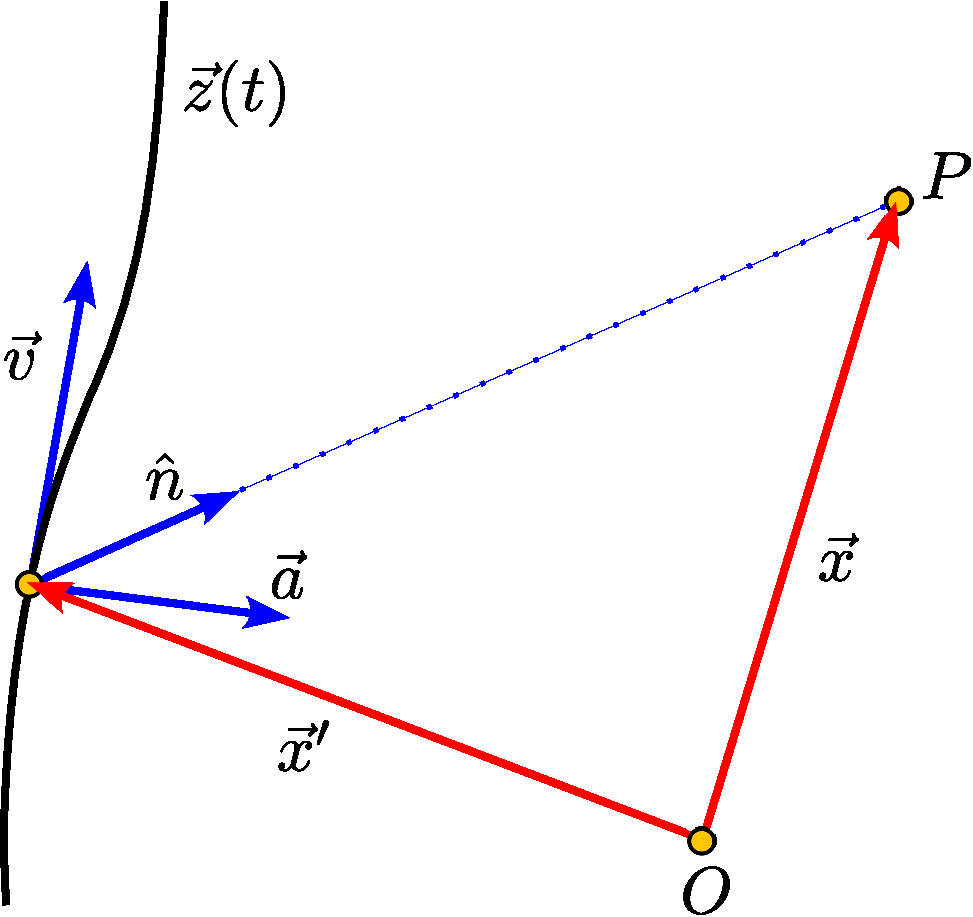
\includegraphics[height=5cm]{fig/fig-vectores.pdf}}
\label{R7}
\end{figure}
Sabemos que los campos el'ectrico y magn'etico est'an dados en t'erminos de derivadas de los potenciales de acuerdo a las expresiones \eqref{defA2} y \eqref{defphi2}. Para evaluar las derivadas involucradas es necesario tener en cuenta que los potenciales retardados dependen de la posici'on $\vec{x}$ y el tiempo $t$ expl'icitamente a trav'es de $\vec{R}=\vec{x}-\vec{z}(t')$ y $\vec{n}$, \textit{pero adem'as impl'icitamente a trav'es del tiempo retardado} $t'=t'(\vec{x},t)$, que es soluci'on de \eqref{t'}.

Tomando en cuenta esta doble dependencia, calculamos:
\begin{eqnarray}
 \partial_i\phi&=&\frac{q}{4\pi\varepsilon}\partial_i\left[\frac{1}{R-\vec{\beta}\cdot\vec{R}}\right] \\
&=&-\frac{q}{4\pi\varepsilon}\frac{1}{(R-\vec{\beta}\cdot\vec{R})^2}\left[\partial_iR-\frac{1}{c}a_j(t')R_j\partial_i t'-\beta_j\partial_iR_j\right].
\end{eqnarray}
Derivando $R^2=R_jR_j$ encontramos que
\begin{equation}
\partial_i R=\hat{n}_j\partial_i R_j. \label{diR}
\end{equation}
Por otro lado, la definici'on (\ref{defR}a) implica que
\begin{equation}
 \partial_i R_j=\partial_i( x_j-z_j(t'))=\delta_{ij}-c\beta_j\partial_i t' . \label{diRj}
\end{equation}
Adem'as, la condici'on (\ref{t'}) permite escribir las derivadas de $t'$ en t'erminos de las derivadas de $R$:
\begin{equation}
 \partial_i t'=\partial_i(t-\frac{1}{c}R)=-\frac{1}{c}\partial_iR. \label{dit'}
\end{equation}
Reemplazando (\ref{diR}) en (\ref{dit'})  y luego usando (\ref{diRj}) obtenemos
\begin{equation}
 \partial_i t'=-\frac{1}{c}\hat{n}_i+(\vec{\beta}\cdot\hat{n})\partial_it', \label{dit'2}
\end{equation}
que nos permite encontrar una expresi'on para $\partial_it'$ en t'erminos de $\hat{n}$ y $\vec{\beta}$:
\begin{equation}
 \boxed{\partial_i t'=-\frac{1}{c}\frac{\hat{n}_i}{1-\vec{\beta}\cdot\hat{n}}.}
\end{equation}
Reemplazando este resultado en (\ref{diRj}) y en (\ref{diR}) obtenemos expresiones similares para las otras derivadas que necesitamos:
\begin{equation}
 \boxed{\partial_i R_j=\delta_{ij}+\frac{\beta_j\hat{n}_i}{1-\vec{\beta}\cdot\hat{n}},}
\end{equation}
\begin{equation}
\boxed{\partial_i R=\frac{\hat{n}_i}{1-\vec{\beta}\cdot\hat{n}}.}
\end{equation}
Con esta informaci'on, podemos expresar el gradiente del potencial escalar como
\begin{equation}
 \partial_i\phi=-\frac{q}{4\pi\varepsilon}\frac{1}{(R-\vec{\beta}\cdot\vec{R})^2} \left[\frac{\hat{n}_i}{1-\vec{\beta}\cdot\hat{n}}+\frac{1}{c^2}\frac{(\vec{a}\cdot\vec{R})\hat{n}_i}{1-\vec{\beta}\cdot\hat{n}} -\beta_i-\frac{\beta^2\hat{n}_i}{1-\vec{\beta}\cdot\hat{n}}\right],
\end{equation}
o, en notaci'on vectorial,
\begin{equation}
 \vec\nabla\phi=-\frac{q}{4\pi\varepsilon}\frac{1}{(R-\vec{\beta}\cdot\vec{R})^2}\left[\frac{\hat{n}}{\gamma^2(1-\vec{\beta}\cdot\hat{n})}+\frac{1}{c^2}\frac{(\vec{a}\cdot\vec{R})\hat{n}}{1-\vec{\beta}\cdot\hat{n}}-\vec\beta\right].
\end{equation}
Similarmente, calculamos la derivada temporal del potencial vectorial:
\begin{eqnarray}
 \partial_t A_i&=&\frac{q\mu c}{4\pi}\partial_t\left[\frac{\beta_i}{R-\vec{\beta}\cdot\vec{R}}\right] \\
&=&\frac{q\mu c}{4\pi}\left[\frac{1}{c}\frac{a_i\partial_tt'}{(R-\vec{\beta}\cdot\vec{R})}-\frac{\beta_i}{(R-\vec{\beta}\cdot\vec{R})^2}\left(\partial_tR-\frac{1}{c}a_j(t')R_j\partial_t t'-\beta_j\partial_tR_j\right)\right] \\
&=&\frac{\mu c}{4\pi}\frac{q}{(R-\vec{\beta}\cdot\vec{R})^2}\left[\frac{1}{c}a_i(R-\vec{\beta}\cdot\vec{R})\partial_tt'-\beta_i\partial_tR+\frac{1}{c}\beta_ia_jR_j\partial_t t'+\beta_i\beta_j\partial_tR_j\right] . \label{dtA}
\end{eqnarray}
Las derivadas del lado derecho de la expresi'on anterior pueden calcularse usando el mismo m'etodo antes usado: Derivando $R^2=R_jR_j$, (\ref{defR}a) y (\ref{t'}) encontramos, respectivamente, que
\begin{equation}
\partial_t R=\hat{n}\cdot\partial_t \vec{R}, \label{dtR}
\end{equation}
\begin{equation}
 \partial_t \vec{R}=\partial_t( \vec{x}-\vec{z}(t'))=-c\vec{\beta}\,\partial_t t', \label{dtRj}
\end{equation}
\begin{equation}
 \partial_t t'=\partial_t(t-\frac{1}{c}R)=1-\frac{1}{c}\partial_tR. \label{dtt'}
\end{equation}
Sustituyendo (\ref{dtR}) en (\ref{dtt'})  y luego usando (\ref{dtRj}) llegamos a
\begin{equation}
 \partial_t t'=1+(\vec{\beta}\cdot\hat{n})\partial_tt',
\end{equation}
de donde podemos despejar $\partial_t t'$, obteniendo
\begin{equation}
 \boxed{\partial_t t'=\frac{1}{1-\vec{\beta}\cdot\hat{n}}.} \label{dtt'2}
\end{equation}
Con esto, (\ref{dtRj}) y (\ref{dtR}) determinan las derivadas faltantes:
\begin{equation}
 \boxed{\partial_t \vec{R}=-\frac{c\vec\beta}{1-\vec{\beta}\cdot\hat{n}},}
\end{equation}
\begin{equation}
\boxed{\partial_t R=-\frac{c(\vec\beta\cdot\hat{n})}{1-\vec{\beta}\cdot\hat{n}}.}
\end{equation}
Sustituci'on en (\ref{dtA}) conduce entonces a
\begin{eqnarray}
 \partial_t \vec{A}
&=&\frac{\mu c}{4\pi}\frac{q}{(R-\vec{\beta}\cdot\vec{R})^2}\left[\frac{1}{c}\vec{a}R+\frac{1}{c}
\frac{\vec{\beta}(\vec{a}\cdot\vec{R})}{(1-\vec{\beta}\cdot\hat{n})}+\frac{c\vec\beta}{1-\vec{\beta}\cdot\hat{n}}(\vec{\beta}\cdot\hat{n}-\beta^2)\right] \\
&=&\frac{\mu c}{4\pi}\frac{q}{(R-\vec{\beta}\cdot\vec{R})^2}\left[\frac{1}{c}\vec{a}R+\frac{1}{c}
\frac{\vec{\beta}(\vec{a}\cdot\vec{R})}{(1-\vec{\beta}\cdot\hat{n})}-c\vec\beta+\frac{c\vec\beta}{\gamma^2(1-\vec{\beta}\cdot\hat{n})}\right] \\
&=&\frac{1}{4\pi\varepsilon}\frac{q}{(R-\vec{\beta}\cdot\vec{R})^2}\left[\frac{1}{c^2}\vec{a}R+\frac{1}{c^2}\frac{\vec{\beta}(\vec{a}\cdot\vec{R})}{(1-\vec{\beta}\cdot\hat{n})}-\vec\beta+\frac{\vec\beta}{\gamma^2(1-\vec{\beta}\cdot\hat{n})}\right] .
\end{eqnarray}
Tenemos ahora los ingredientes necesarios para calcular el campo el'ectrico:
\begin{eqnarray}
4\pi\varepsilon\vec{E}&=&\frac{q}{(R-\vec{\beta}\cdot\vec{R})^2}\left[\frac{\hat{n}}{\gamma^2(1-\vec{\beta}\cdot\hat{n})}+\frac{1}{c^2}\frac{(\vec{a}\cdot\vec{R})\hat{n}}{(1-\vec{\beta}\cdot\hat{n})}-\vec\beta-\frac{1}{c^2}\vec{a}R-\frac{1}{c^2}\frac{\vec{\beta}(\vec{a}\cdot\vec{R})}{(1-\vec{\beta}\cdot\hat{n})}+\vec\beta-\frac{\vec\beta}{\gamma^2(1-\vec{\beta}\cdot\hat{n})}\right] \nonumber \\
&=&\frac{q}{(R-\vec{\beta}\cdot\vec{R})^2}\left[\frac{\hat{n}-\vec\beta}{\gamma^2(1-\vec{\beta}\cdot\hat{n})}+\frac{1}{c^2}\frac{(\vec{a}\cdot\vec{R})\hat{n}}{(1-\vec{\beta}\cdot\hat{n})}-\frac{1}{c^2}\vec{a}R-\frac{1}{c^2}\frac{\vec{\beta}(\vec{a}\cdot\vec{R})}{(1-\vec{\beta}\cdot\hat{n})}\right] \\
&=&\frac{q(\hat{n}-\vec\beta)}{\gamma^2R^2(1-\vec{\beta}\cdot\hat{n})^3}+\frac{q}{c^2(R-\vec{\beta}\cdot\vec{R})^2}\left[\frac{(\vec{a}\cdot\vec{R})\hat{n}}{(1-\vec{\beta}\cdot\hat{n})}-\vec{a}R-\frac{\vec{\beta}(\vec{a}\cdot\vec{R})}{(1-\vec{\beta}\cdot\hat{n})}\right] \\
&=&\frac{q(\hat{n}-\vec\beta)}{\gamma^2R^2(1-\vec{\beta}\cdot\hat{n})^3}+\frac{q}{c^2R^2(1-\vec{\beta}\cdot\hat{n})^3}\left[(\vec{a}\cdot\vec{R})\hat{n}-\vec{a}R+\vec{a}\vec{\beta}\cdot\vec{R}-\vec{\beta}(\vec{a}\cdot\vec{R})\right] \\
&=&\frac{q(\hat{n}-\vec\beta)}{\gamma^2R^2(1-\vec{\beta}\cdot\hat{n})^3}+\frac{q}{c^2R(1-\vec{\beta}\cdot\hat{n})^3}\left[(\vec{a}\cdot\hat{n})(\hat{n}-\vec{\beta})-\vec{a}+\vec{a}\vec{\beta}\cdot\hat{n}\right] .
\end{eqnarray}
Usando la identidad
\begin{equation}
(\vec{a}\cdot\hat{n})(\hat{n}-\vec{\beta})-\vec{a}+\vec{a}\vec{\beta}\cdot\hat{n}\equiv (\vec{a}\cdot\hat{n})(\hat{n}-\vec{\beta})-\vec{a} (1-\hat{n}\cdot\vec\beta)\equiv \hat{n}\times\left[ \left( \hat{n}-\vec{\beta}\right)
\times{\vec{a}}\right],
\end{equation}
encontramos finalmente que\textit{ el campo el'ectrico generado por una carga $q$ en movimiento arbitrario} es de la forma
\begin{equation}\marginnote{campo $\vec{E}$ carga $q$}
\boxed{\vec{E}(\vec{x},t)=\vec{E}_{(1)}+\vec{E}_{(2)}=\frac{q}{4\pi\varepsilon}\left.\frac{\left(
\hat{n}-\vec{\beta}\right)
}{\gamma^2R^2\left(1-\vec{\beta}\cdot\hat{n}\right)^3}\right|_{\rm ret}+
\frac{q\mu}{4\pi}\left.\frac{\hat{n}\times\left[ \left( \hat{n}-\vec{\beta}\right)
\times{\vec{a}}\right] }{R\left( 1-\vec{\beta}\cdot\hat{n}\right)
^3}\right|_{\rm ret} .} \label{Egen}
\end{equation}
El campo magn'etico puede calcularse de forma similar, encontr'andose que \textit{puede expresarse completamente en t'erminos del campo el'ectrico}:
\begin{equation}\marginnote{campo $\vec{B}$ carga $q$}
\boxed{\vec{B}(\vec{x},t)=\frac{1}{c}\left. \hat{n}\right|_{\rm
ret}\times\vec{E}(\vec{x},t) .}
\end{equation}
Este resultado muestra, por lo tanto, que \textit{el campo magn'etico producido por una carga puntual es, en cada punto del espacio, perpendicular al campo el'ectrico y al vector que une la posici'on \underline{retardada} de la carga con el punto de observaci'on}.

Note que para distancias $r$ muy grandes (comparadas con las dimensiones de la
regi'on donde se encuentran las fuentes, que consideramos una regi'on compacta) $R\approx r$ y entonces
$\vec{E}_{(1)}\propto r^{-2}$ mientras que $\vec{E}_{(2)}\propto
r^{-1}$.


\section{Potencia Radiada}

Consideramos un sistema de cargas y corrientes confinado a una regi'on compacta del espacio (por ejemplo, la carga puntual analizada en la secci'on anterior). El campo electromagn'etico que este sistema produce tiene asociado un vector de flujo de energ'ia, el vector de Poynting. La potencia (es decir, la energ'ia por unidad de tiempo) total transferida por el campo electromagn'etico generado por las cargas y corrientes, a trav'es de una superficie que encierra completamente al sistema, y elegida por conveniencia como una esfera de radio $r$, es dada por
\begin{equation}
P(r,t)=\int_S \vec{S}\cdot d\vec{S}=\frac{1}{\mu}\int_S \left[ \left(
\vec{E}\times\vec{B}\right) \cdot \hat{r}\right] \,r^2d\Omega.
\end{equation}

Llamamos \textbf{potencia radiada} a la energ'ia que es transportada \textit{muy lejos} de las fuentes, es decir $r\gg L$ donde $L$ es el tama\~no (lineal) caracter'istico del sistema, y que \textit{aproximamos} por el l'imite en que $r\rightarrow\infty$. En este l'imite, ubicando el centro de la esfera en un punto representativo de la distribuci'on de cargas y corrientes, podemos aproximar $\hat{n}\approx\hat{r}$ y $R\approx r$ de modo que,
\begin{equation}
P_{\rm rad} (t)=\lim_{r\rightarrow\infty}\frac{1}{\mu}\int_S \left[ \left(
\vec{E}\times\vec{B}\right) \cdot \hat{n}\right] \,r^2 d\Omega.
\end{equation}

Tomando en cuenta la dependencia de $\vec{E}_{(1)}$ y $\vec{E}_{(2)}$ con $r$
podemos ver que s'olo los t'erminos provenientes de $\vec{E}_{(2)}$
contribuir'an a $P_{\rm rad}(t)$ en el l'imite $r\rightarrow\infty$, es decir,
\begin{equation}\label{Pinf1}
P_{\rm rad}(t)=\lim_{r\rightarrow\infty}\int_S \vec{S}_{(2)}\cdot
d\vec{S}=\frac{1}{\mu}\lim_{r\rightarrow\infty}\int_S \left[ \left(
\vec{E}_{(2)}\times\vec{B}_{(2)}\right) \cdot \hat{n}\right] \,r^2 d\Omega.
\end{equation}
En otras palabras, el sistema rad'ia energ'ia (``al infinito'') \textit{s'olo si la
carga acelera}. Por esto, $\vec{E}_{(2)}$ recibe el nombre de \textbf{campo de
radiaci'on} o \textbf{campo lejano}, mientras que $\vec{E}_{(1)}$ es llamado
\textbf{campo cercano}.

Calculamos ahora la parte del vector de Poynting que contribuir'a a la energ'ia
radiada fuera del sistema (al infinito):
\begin{equation}
 \vec{S}_{(2)}:=\frac{1}{\mu}\, \vec{E}_{(2)}\times\vec{B}_{(2)},
\end{equation}
con
\begin{equation}
\vec{B}_{(2)}= \frac{1}{c}\hat{n}\times\vec{E}_{(2)}.
\end{equation}
Con estos ingredientes encontramos que
\begin{eqnarray}
 \vec{S}_{(2)}&=&\frac{1}{\mu c}\, \vec{E}_{(2)}\times\left(
\hat{n}\times\vec{E}_{(2)}\right) \\
 &=& \frac{1}{\mu c}\left[ \left|\vec{E}_{(2)}\right|^2 \hat{n}-\left(
\vec{E}_{(2)}\cdot\hat{n}\right)  \vec{E}_{(2)}\right].
\end{eqnarray}
Sin embargo, de (\ref{Egen}) vemos que $\vec{E}_{(2)}$ es normal a $\hat{n}$ de
modo que lo anterior se reduce a
\begin{equation}\label{S2E}
 \boxed{\vec{S}_{(2)}= \frac{1}{\mu c} \left|\vec{E}_{(2)}\right|^2 \hat{n},}
\end{equation}
y por lo tanto
\begin{equation}
 \boxed{P_{\rm rad} (t)=\frac{q^2\mu}{16\pi^2c}\lim_{r\rightarrow\infty}\int_\Omega
\left|\left.\frac{\hat{n}\times\left[ \left( \hat{n}-\vec{\beta}\right)
\times{\vec{a}}\right] }{\left( 1-\vec{\beta}\cdot\hat{n}\right)
^3}\right|_{\rm ret}\right|^2 d\Omega.}
\end{equation}

Definimos la potencia radiada \textit{por unidad de 'angulo s'olido}
por
\begin{equation}
 \boxed{\frac{dP_{\rm rad}}{d\Omega}(\hat{n},t):=\frac{q^2\mu}{16\pi^2c}\lim_{r\rightarrow\infty} \left|\left.
\frac{\hat{n}\times\left[ \left( \hat{n}-\vec{\beta}\right)
\times{\vec{a}}\right] }{\left( 1-\vec{\beta}\cdot\hat{n}\right)
^3}\right|_{\rm ret}\right|^2 ,} \label{dPdO}
\end{equation}
de modo que
\begin{equation}
 \boxed{P_{\rm rad}(t)=\int_\Omega \frac{dP_{\rm rad}}{d\Omega}\,d\Omega.}
\end{equation}


\section{F'ormula de Larmor (no-relativista)}\label{sec:Larmor-norel}

Si $v\ll c$, es decir $\beta\ll1$, entonces el campo el'ectrico
(\ref{Egen}) y la distribuci'on de potencia radiada (\ref{dPdO}) pueden
aproximarse por:
\begin{equation}
\vec{E}(\vec{x},t)=\frac{q\mu}{4\pi}\left.\frac{\hat{n}}{R^2}\right|_{\rm ret}+\left.
\frac{q\mu}{4\pi c^2}\frac{\hat{n}\times(\hat{n}\times{\vec{a}})}{R}\right|_{\rm
ret} +O(\beta),
\end{equation}
\begin{equation}
\frac{dP}{d\Omega}=\frac{q^2\mu}{16\pi^2c}\lim_{r\rightarrow\infty}
\left|\hat{n}\times\left[
\hat{n}\times{\vec{a}}\right]\right|^2_{\rm ret}  +O(\beta).
\end{equation}
Aqu'i $|_{\rm ret}$ denota evaluaci'on de las cantidades en el tiempo retardado, que muy lejos de la fuente adopta la forma $t'=t-r/c$.
Introduciendo el 'angulo $\theta$ entre la aceleraci'on $\vec{a}$ y el vector
normal $\hat{n}$, podemos escribir
$\left|\hat{n}\times\left[\hat{n}\times{\vec{a}}\right]\right|^2=\vec{a}^2\sen^2\theta$ y entonces
\begin{equation}
\frac{dP}{d\Omega}(t)=\frac{q^2\mu}{16\pi^2 c}\left[ \vec{a}^2\sen^2\theta\right]_{\rm
ret} .\label{Lardif}
\end{equation}
 Note que la dependencia $\sen^2\theta$ de ${dP}/{d\Omega}$ implica que \textbf{la
energ'ia radiada se dirige mayoritariamente en la direcci'on normal a la
aceleraci'on}. Adem'as, como $\vec{E}_{(2)}\propto
\hat{n}\times(\hat{n}\times{\vec{a}})$ entonces el campo el'ectrico de
radiaci'on  es normal a $\hat{n}$ y est'a contenido en el plano definido por
$\vec{a}$ y $\hat{n}$. Ver figura \ref{fig:natheta}.
 Decimos entonces que el campo de radiaci'on est'a
\textit{polarizado} en el plano definido por $\vec{a}$ y $\hat{n}$ y es normal a
$\hat{n}$. Si $\vec{a}$ es constante, la radiaci'on emitida en una direcci'on $\hat{n}$ dada tiene polarizaci'on 100\% lineal.
\begin{figure}[!h]
\centerline{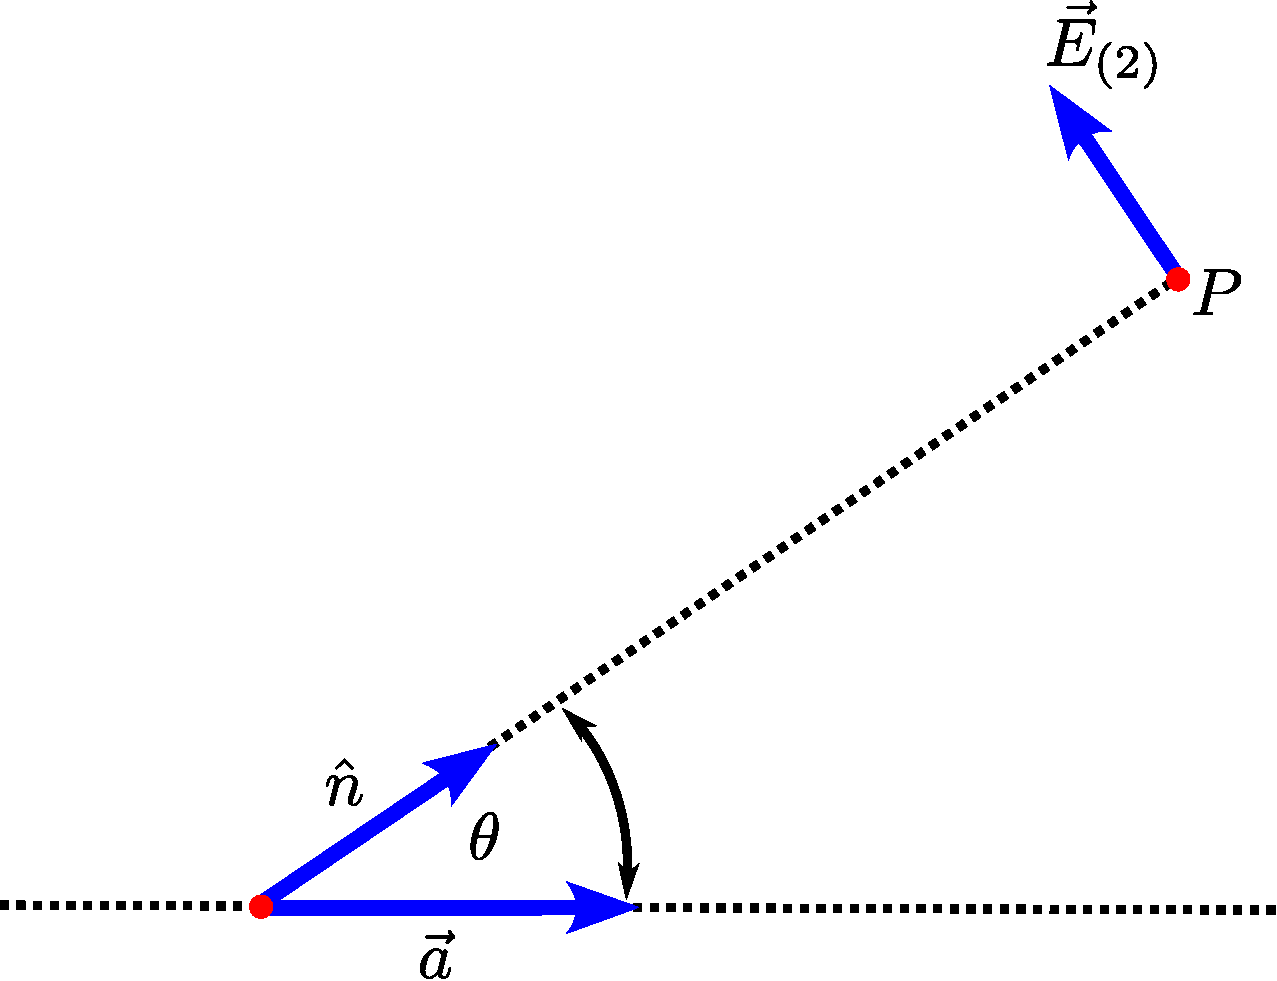
\includegraphics[height=5cm]{fig/fig-a-n-Erad.pdf}}
\caption{Direcciones de la aceleraci'on $\vec{a}$, vector unitario $\hat{n}$ y campo el'ectrico $\vec{E}_{(2)}$.}
\label{fig:natheta}
\end{figure}
En un \textit{gr'afico de distribuci'on de potencia} (donde se usan coordenadas polares
en las que el radio es identificado con ${dP}/{d\Omega}$, que es funci'on
del 'angulo $\theta$) encontramos una distribuci'on como muestra la figura
\ref{lobulo01}. Vemos entonces que en el l'imite no-relativista la mayor
cantidad de la energ'ia es radiada en direcci'on normal a la aceleraci'on de la
carga.

\begin{figure}[!h]
\centerline{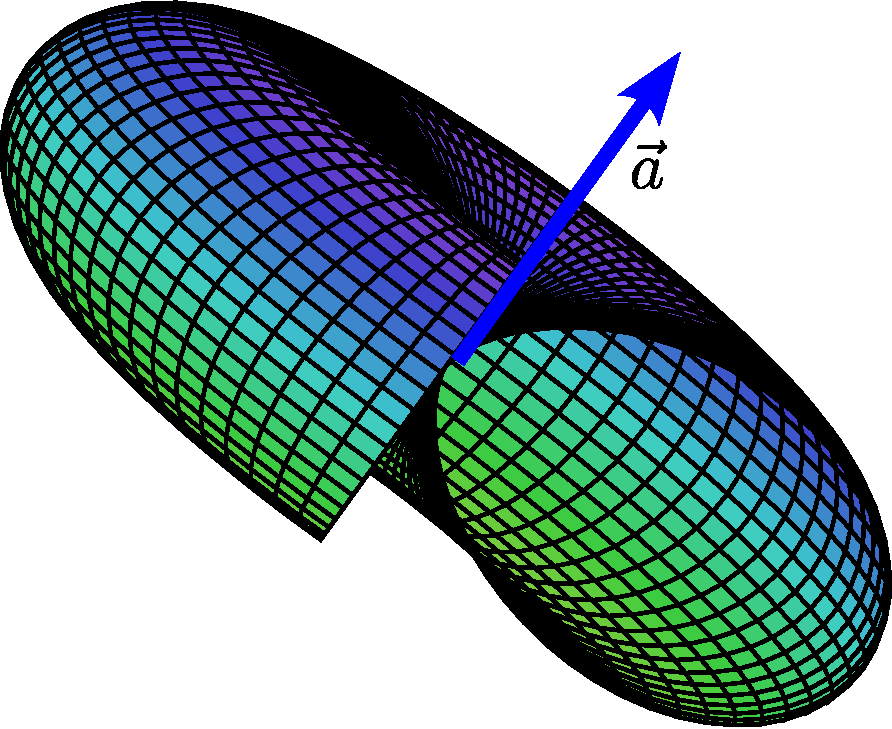
\includegraphics[height=6cm]{fig/fig-Larmor.pdf}\hfill
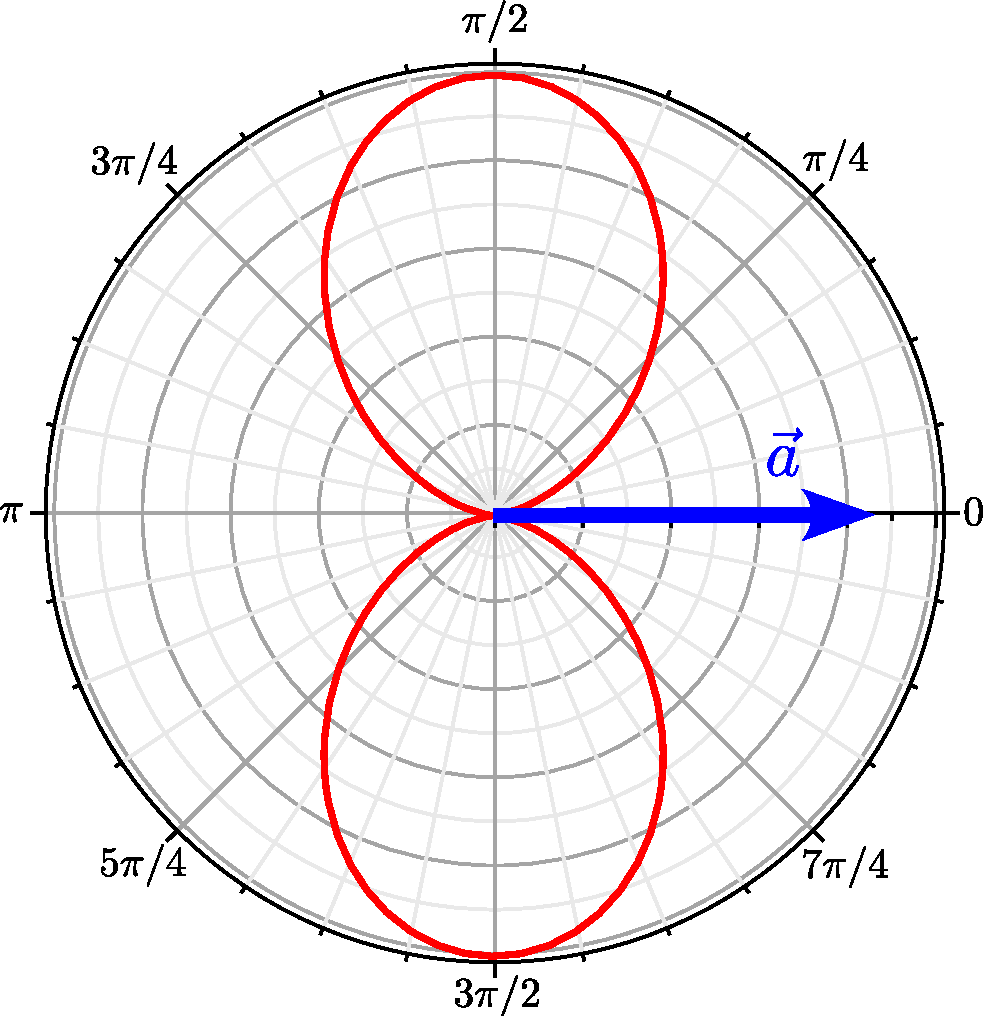
\includegraphics[height=6cm]{fig/fig-Larmor-02.pdf}}
\caption{Distribuci'on de potencia para una carga no-relativista en movimiento
acelerado. C'odigos Python \href{https://github.com/gfrubi/electrodinamica/blob/master/figuras-editables/fig-Larmor-3D.py}{aqu\'i} y \href{https://github.com/gfrubi/electrodinamica/blob/master/figuras-editables/fig-Larmor.py}{aqu\'i}.}
\label{lobulo01}
\end{figure}
La \textit{potencia total emitida} por la carga es entonces
\begin{eqnarray}
P(t)  & =&\int_{\Omega}\frac{dP}{d\Omega}(t)\,d\Omega\\
& =&\frac{q^2\mu}{16\pi^2c}\int_{\Omega} [\vec{a}^2\sen^2\theta]_{\rm ret}\,d\Omega\\
& =&\frac{q^2\mu}{16\pi^2c}\int_0^{\pi}\int_0^{2\pi}\vec{a}^2_{\rm ret}
\sen^2\theta\sen\theta\,d\theta d\varphi \\
& =&\frac{q^2\mu}{16\pi^2c}\,\vec{a}^2_{\rm ret}\, \frac{4}{3}\,2\pi \\
& =&\frac{q^2\mu}{6\pi c}\,\vec{a}^2_{\rm ret}.
\end{eqnarray}
Este resultado es conocido como \emph{f'ormula de Larmor}\footnote{Joseph Larmor (1857-1942): f'isico y matem'atico irland'es. Ver \url{http://es.wikipedia.org/wiki/Joseph_Larmor}.}.
%\begin{equation}
%\boxed{P=\frac{2q^2}{3c^3}\,\vec{a}^2.}\label{R-larmor}
%\end{equation}
\begin{equation}\marginnote{F'ormula de Larmor}
\boxed{P(t)=\frac{q^2\mu}{6\pi c}\,\vec{a}^2_{\rm ret}.}\label{R-larmor}
\end{equation}

Este importante resultado implica, en particular, que cargas de igual magnitud, pero masas distintas sometidas a la acci'on de una misma fuerza (o fuerzas de igual magnitud) rad'ian con potencias distintas si sus masas son distintas. Por ejemplo, \textit{en un sistema formado por protones y electrones, acelerados bajo la acci'on de un mismo campo el'ectrico externo, ser'an los electrones quienes m'as energ'ia radiar'an} puesto que, si bien sus cargas son iguales en m'odulo, la masa de los electrones es mucho menor que la de los protones ($m_{\rm p}\approx 1836\,m_{\rm e}$, ver ap'endice \ref{app:constantes}. Por lo tanto, $P_{\rm e}\approx 3\times 10^6\, P_{\rm p}$). Como consecuencia, en \textit{primera aproximaci'on, son los electrones los principales responsables de la radiaci'on emitida por un sistema}.

%\subsubsection{Ejemplo: Movimiento circular}

\section{Distribuci'on de potencia (correcci'on relativista)}
La energ'ia radiada (muy lejos de la regi'on donde se mueve la carga) es dada por 
\begin{equation}
 E=\int_t\oint_\Omega \frac{dP}{d\Omega}\,d\Omega\,dt=\frac{q^2\mu}{16\pi^2 c}\oint_\Omega\int_t\left.\frac{\left|\hat{n}\times
\left[ \left( \hat{n}-\vec{\beta}\right)\times{\vec{a}}\right]\right|^2}{\left(
1-\hat{n}\cdot\vec{\beta}\right) ^{6}}\right|_{\rm ret}\,dt\,d\Omega .
\end{equation}
Considere el caso particular en que \textit{la carga acelera s'olo en un cierto intervalo de tiempo}, por ejemplo, $\vec{a}(t)\neq\vec{0}$ s'olo entre $t=T_1$ y $t=T_2$. La radiaci'on emitida es entonces causada por la aceleraci'on de la carga en ese periodo de tiempo. Sin embargo, debido a que el integrando est'a evaluado en el tiempo retardado $t'(\vec{x},t)$, el intervalo de tiempo en que se realiza la integraci'on (\ref{Ecasi}) para calcular la energ'ia radiada  (``muy lejos'') difiere del intervalo de tiempo en que la carga aceler'o. 'Esta es una consecuencia de la velocidad finita ($c$) de propagaci'on de las se\~nales electromagn'eticas. En el ejemplo particular analizado, la contribuci'on a la integral s'olo ser'a no nula en un intervalo de tiempo entre $t=t_1$ y $t=t_2$, de modo que
\begin{equation}
 E=\frac{q^2\mu}{16\pi^2 c}\oint_\Omega\int_{t_1}^{t_2}\left.\frac{\left|\hat{n}\times
\left[ \left( \hat{n}-\vec{\beta}\right)\times{\vec{a}}\right]\right|^2}{\left(
1-\hat{n}\cdot\vec{\beta}\right) ^{6}}\right|_{\rm ret}\,dt\,d\Omega , \label{Ecasi}
\end{equation}
y donde los valores $t_1$ y $t_2$ est'an relacionados con $T_1$ y $T_2$ por medio de
\begin{eqnarray}
T_1=t'(\vec{x},t_1)=t_1-\frac{1}{c}|\vec{x}-\vec{z}(T_1)|
\approx t_1-\frac{r}{c}, \\
T_2=t'(\vec{x},t_2)=t_2-\frac{1}{c}|\vec{x}-\vec{z}(T_2)|
\approx t_2-\frac{r}{c},
\end{eqnarray}
es decir, que $T_1$ y $T_2$ son los tiempos retardados asociados a los tiempos $t_1$ y $t_2$. Aqu'i hemos considerado que $r=|\vec{x}|\gg |\vec{z}(t)|$. Ver figura \ref{fig:tiempos}.
\begin{figure}[H]
\centerline{\includegraphics[height=1.5cm]{fig/fig-tiempos.pdf}}
\caption{Tiempos retardados y tiempos de observaci'on.}
\label{fig:tiempos}
\end{figure}

En resumen, si bien la carga acelera s'olo en el intervalo de tiempo $[T_1,T_2]$, la integral \eqref{Ecasi} para la energ'ia radiada se extiende sobre un intervalo de tiempo diferente (y posterior) $[t_1,t_2]$. En la mayor'ia de las situaciones es m'as conveniente calcular la energ'ia radiada de modo que se integre \textit{directamente en el intervalo de tiempo correspondiente al periodo en que la carga acelera}. Esto equivale a realizar, \textit{para un valor de $\vec{x}'$ fijo dentro de la integral sobre el 'angulo s'olido en \eqref{Ecasi}},  un cambio de variable de $t$ a $t'$, es decir, a escribir
\begin{equation}
 E=\frac{q^2\mu}{16\pi^2 c}\oint_\Omega\int_{T_1}^{T_2}\left.\frac{\left|\hat{n}\times
\left[ \left( \hat{n}-\vec{\beta}\right)\times{\vec{a}}\right]\right|^2}{\left(
1-\hat{n}\cdot\vec{\beta}\right) ^{6}}\right|_{t'}\left(\frac{dt}{dt'}\right)\,dt'd\Omega .\label{Edt'}
\end{equation}
En el cambio de variable anterior las coordenadas espaciales no son variadas, de modo que
\begin{equation}
\frac{dt}{dt'}=\left[\left(\frac{\partial t'}{\partial t}\right)_{\vec{x}=\text{cte.}}\right]^{-1}
=\left[\partial_t t'\right]^{-1}=1-\hat{n}\cdot\vec{\beta}. \label{dtdt'}
\end{equation}
En la 'ultima igualdad hemos usado nuestro resultado (\ref{dtt'2}). Note que esto implica que $dt<dt'$ \textit{si la velocidad de la carga est'a dirigida en la misma direcci'on que el vector} $\vec{n}$ (que apunta desde la carga hasta el punto lejano de observaci'on) y $dt>dt'$ \textit{en caso contrario}. Esta diferencia de intervalos de tiempo corresponde al simple efecto cinem'atico en virtud del cual  la duraci'on de una se\~nal emitida por una fuente luminosa en movimiento es percibida como menor si la fuente se mueve hacia el receptor, y viceversa (efecto Doppler).

Reemplazando (\ref{dtdt'}) en (\ref{Edt'}) obtenemos
\begin{equation}
 E=\frac{q^2\mu}{16\pi^2 c}\oint_\Omega\int_{T_1}^{T_2}\left.\frac{\left|\hat{n}\times\left[ \left( \hat{n}-\vec{\beta}\right)\times{\vec{a}}\right]\right|^2}{\left(1-\hat{n}\cdot\vec{\beta}\right)^5}\right|_{t'}\,dt'd\Omega .\label{Edt'2}
\end{equation}

Ahora \textit{el integrando est'a evaluado en el mismo tiempo usado para la integraci'on}, y por lo tanto s'olo contribuye integrar sobre el intervalo de tiempo en el cual la carga acelera. Puede decirse que la integral (\ref{Edt'2}) permite calcular la energ'ia que \textit{ser'a irradiada} por la carga debido a su movimiento (aceleraci'on) en el intervalo $[T_1,T_2]$.

Podemos consecuentemente definir una correspondiente potencia irradiada por unidad de 'angulo s'olido:
\begin{equation}
\boxed{\frac{dP'}{d\Omega}(t):=\frac{q^2\mu}{16\pi^2 c}\frac{\left|\hat{n}\times
\left[ \left( \hat{n}-\vec{\beta}\right)\times{\vec{a}}\right]\right|^2}{\left(
1-\hat{n}\cdot\vec{\beta}\right) ^{5}},} \label{dP'}
\end{equation}
de modo que
\begin{equation}
 \boxed{E=\int_\Omega\int_{T_1}^{T_2}\frac{dP'}{d\Omega}(t)\,dt\,d\Omega}
\end{equation}
es la energ'ia (\textit{que ser'a}) radiada por la carga, debido a su movimiento entre los tiempos $T_1$ y $T_2$ (es decir, con posici'on inicial $\vec{z}(T_1)$ y final $\vec{z}(T_2)$, etc).

Resumiendo: la potencia (por unidad de 'angulo s'olido) (\ref{dP'}) se diferencia de (\ref{dPdO}) en que la 'ultima es la energ'ia radiada (por unidad de 'angulo s'olido) \textit{por unidad de tiempo transcurrido en los puntos (muy lejanos) de observaci'on}, mientras que (\ref{dP'}) es la energ'ia (que ser'a) radiada (por unidad de 'angulo s'olido) \textit{por unidad de tiempo transcurrido en el movimiento de la carga}. Si bien la energ'ia total radiada dada por las expresiones \eqref{Ecasi} y \eqref{dP'} es la misma, en la mayor'ia de las aplicaciones\footnote{...donde las velocidades de las cargas son relativistas, de otro modo la diferencia es insignificante.} es m'as conveniente describir la distribuci'on de potencia radiada usando \eqref{dP'}.

\subsubsection{Ejemplo: Movimiento unidimensional}
\begin{figure}[!h]
\centerline{\includegraphics[height=4cm]{fig/fig-movimiento_lineal.pdf}}
\caption{Geometr'ia para un movimiento unidimensional acelerado.}
\label{R14}
\end{figure}
En este caso de movimiento unidimensional acelerado tenemos que la velocidad es paralela a la aceleraci'on, de modo que $\vec{\beta}\times\vec{a}=\vec{0}$. Adem'as,
$\hat{n}\cdot\vec{\beta}=\beta\cos\theta$.
Reemplazando esto en \eqref{dP'} encontramos que 
\begin{equation}
\frac{dP'}{d\Omega}=\frac{\mu q^2}{16\pi^2 c}\frac{\vec{a}^2\sen^2
\theta}{\left(1-\beta\cos\theta\right)^5}. \label{dppdO}
\end{equation}
\begin{figure}[H]
\centerline{\includegraphics[height=6cm]{fig/fig-carga-relativista.pdf}}
\caption{L'obulos de radiaci'on para una carga relativista acelerada. Suponemos
iguales aceleraciones y normalizamos con respecto a ${\mu q^2\vec{a}^2}/{16\pi^2 c}$. C'odigo Python \href{https://github.com/gfrubi/electrodinamica/blob/master/figuras-editables/fig-carga-relativista.py}{aqu\'i}.}
\label{lobulo02}
\end{figure}
Podemos encontrar el 'angulo $\theta=\theta_{\rm max}$ en el que se emite el
\textit{m'aximo de radiaci'on}. Derivando (\ref{dppdO}) con respecto a $\theta$ e
igualando a cero, encontramos que
\begin{equation}
\cos\theta_{\rm max}=\frac{1}{3\beta}\left\{  \sqrt{1+15\beta^2}-1\right\}  .
\end{equation}
Esto indica que, para la misma aceleraci'on, la radiaci'on emitida por una carga se concentra m'as y m'as en la direcci'on de movimiento, a medida que la velocidad de la carga es mayor.


\section{Scattering de Thomson}
%Thomson=por carga, clasicamente elastico (igual frecuencia), intensidad indep. de frecuencia.
%Compton= igual que Thomson, pero tomando en cuenta efecto Compton = corrimiento frecuencia, para energías altas (comparables a energía en reposo de carga)
%Rayleigh=por particulas neutras pequeñas comparadas con \lambda: moleculas (aire), elastico = dipolos = intensidad depende de frec^4. Ejemplo, difusión de luz solar en moléculas de la atmósfera.
%Mie = cuerpos neutros grandes comparados con \lambda
%Raman=inelastico, absorbe/emite energia de modos de excitación de un sólido o líquido.


%*** AGREGAR: Introducir Intensidad $I$ de radiacion (pot/area)

Si una onda electromagn'etica monocrom'atica incide
sobre una part'icula libre de carga $q$ y masa $m$, la carga acelera y
entonces emite radiaci'on. Esta radiaci'on ser'a emitida en otras
direcciones respecto de la direcci'on de la onda incidente. Adem'as, si la carga se mueve a velocidades no-relativistas la radiaci'on emitida por esta carga tendr'a \textit{casi exclusivamente} la misma frecuencia que la radiaci'on incidente (ver secci'on \ref{sec:rfp} para mayores detalles). El proceso completo puede ser descrito como \textit{scattering} (dispersi'on) \textit{esl'astico} de la radiaci'on incidente, que llamamos \textbf{scattering de Thomson}\footnote{Joseph John Thomson (1856-1940): f'isico brit'anico. Ver \url{http://es.wikipedia.org/wiki/Joseph_John_Thomson}.}.

La potencia instant'anea radiada es dada por (\ref{Lardif}) o, introduciendo el
\textbf{vector de polarizaci'on $\vec{\epsilon}$ de la onda emitida} (que es, por definici'on, el vector unitario paralelo a la direcci'on del campo el'ectrico radiado, ver figura \ref{fig:natheta}):
\begin{equation}
\frac{dP}{d\Omega}=\frac{q^2\mu}{16\pi^2 c}|\hat{n}\times\vec{a}|^2.
\end{equation}
En este caso, la aceleraci'on es producida por la fuerza que la onda incidente ejerce sobre la carga. Si la onda incidente es \textit{plana y polarizada linealmente}, con vector de onda $\vec{k}_0$ y vector de polarizaci'on $\vec{\epsilon}_0$, su campo el'ectrico puede ser descrito usando
\begin{equation}
\vec{E}_0(\vec{x},t)=\operatorname{Re}\left[
\vec{\epsilon}_0E_0e^{i(\vec{k}_0\cdot\vec{x}-\omega t)}\right] .
\end{equation}
\textit{Suponiendo que la velocidad de la carga es en todo momento mucho menor que la de la luz}, podemos despreciar el t'ermino dependiente del campo magn'etico en la fuerza de Lorentz. Entonces, la aceleraci'on de la carga es proporcional al campo el'ectrico de la onda incidente:
\begin{equation}\label{ecd2x}
\frac{d^2\vec{x}}{dt^2}
=\operatorname{Re}\left[\frac{qE_0}{m}\vec{\epsilon}_0e^{i(\vec{k}_0\cdot\vec{x}(t)
-\omega t)}\right] .
\end{equation}
Considerando las condiciones iniciales $\vec{x}(0)=\vec{0}$ y $\vec{v}(0)=\vec{0}$, integramos esta ecuaci'on diferencial\footnote{Note que la inc'ognita, $\vec{x}(t)$, aparece en el t'ermino exponencial al lado derecho de \eqref{ecd2x}, por lo que la solci'on es, para condiciones iniciales generales, bastante no-trivial.} y obtenemos que la posici'on y velocidad de la carga tienen la forma
\begin{equation}
\vec{x}(t)
=\operatorname{Re}\left[-\frac{qE_0}{m\omega^2}\vec{\epsilon}_0(e^{-i\omega t}-1)\right] ,
\end{equation}
\begin{equation}
\vec{v}(t)
=\operatorname{Re}\left[i\frac{qE_0}{m\omega}\vec{\epsilon}_0e^{-i\omega t}\right] .
\end{equation}
Vemos de aqu'i que las amplitudes de las oscilaciones en posici'on y velocidad son
$A={qE_0}/{m\omega^2}$ y $v_{\max}={qE_0}/{m\omega}$. Por lo
tanto, la aproximaci'on usada es consistente s'olo si $v_{\max}\ll c$, es decir si
$E_0\ll {m\omega c}/{q}$. Ya que $A={v_{\max}}/{\omega}$, esta condici'on
es equivalente a $A\ll c/\omega=\lambda/2\pi$, es decir, a que \textit{la amplitud de la oscilaci'on de la carga sea mucho menor que la longitud de onda (reducida) de la radiaci'on incidente}.

Es conveniente calcular el flujo de energ'ia promedio irradiado en un ciclo,
para lo cual requerimos el promedio $\left\langle
{dP}/{d\Omega}\right\rangle$ en un periodo:
\begin{eqnarray}
\left\langle\frac{dP}{d\Omega}\right\rangle  &=&
\frac{q^2\mu}{16\pi^2 c}\left\langle |\hat{n}\times\vec{a}|^2\right\rangle \\
&=&\left(\frac{q^2\mu}{16\pi^2 c}\right)\left(\frac{qE_0}{m}\right)^2\left|
\hat{n}\times\vec{\epsilon}_0\right|^2\left\langle
\cos^2(\omega t)\right\rangle \\
&=&\left(\frac{q^4\mu E_0^2}{32\pi^2 c m^2}\right)\left|
\hat{n}\times\vec{\epsilon}_0\right|^2\\
&=&\left(\frac{q^2\mu}{4\pi m}\right)^2\left(\frac{E_0^2}{2\mu c}\right) \left|
\hat{n}\times\vec{\epsilon}_0\right|^2.
\end{eqnarray}
En la pr'actica es conveniente describir este proceso de scattering por medio de
la correspondiente  \textbf{secci'on diferencial de scattering}:
\begin{equation}
\frac{d\sigma}{d\Omega}:=\frac{\left( \text{Energ'ia promedio radiada por unidad
de tiempo y de 'angulo s'olido}\right) }{\left( \text{Energ'ia promedio
incidente por unidad de 'area y de tiempo}\right) }=\frac{\left\langle
\frac{dP}{d\Omega}\right\rangle}{\left\langle S_0\right\rangle}.
\end{equation}
Note que ${d\sigma}/{d\Omega}$ tiene unidades de 'area (por unidad de 'angulo
s'olido).
El flujo de energ'ia incidente promedio es precisamente el vector de Poynting
del campo incidente, promediado en un periodo, y est'a dado por la expresi'on \eqref{Sprom}:
\begin{eqnarray}
\left\langle S_0\right\rangle &=&\frac{1}{2\mu c}E_0^2.
\end{eqnarray}
Obtenemos entonces que la secci'on diferencial de scattering es dada por
\begin{equation}
\boxed{\frac{d\sigma}{d\Omega}  =\left(\frac{q^2\mu}{4\pi m}\right)^2\left|
\hat{n}\times\vec{\epsilon}_0\right|^2 .}\label{seeT}
\end{equation}
La cantidad $r_q:={q^2\mu}/{4\pi m}=(1/{4\pi\varepsilon})({q^2}/{mc^2})$ tiene dimensiones de longitud, y juega el rol de ``\textit{tama\~no efectivo}'' de la carga para el proceso de scattering considerado\footnote{Compare, por ejemplo, con la secci'on diferencial de scaterring de una esfera de radio $R$ impactada por peque\~nas part'iculas de prueba (de masa despreciable): $d\sigma/d\Omega=R^2/4$, $\sigma=\pi R^2$.}. Por ejemplo, para el electr'on en el vac'io $r_{\rm e}=(1/{4\pi\varepsilon_0})({e^2}/{m_{\rm e}c^2})\approx 2,8\times 10^{-15}m$. Esta distancia caracter'istica (de la interacci'on electromagn'etica) del electr'on es llamada \textbf{radio cl'asico del electr'on}.

Para evaluar (\ref{seeT}) requerimos de una expresi'on expl'icita para
$\left|\hat{n}\times\vec{\epsilon}_0\right|^2$. El c'alculo es m'as sencillo si elegimos los ejes coordenados de modo que el vector de onda inicial $\vec{k}_0$ sea paralelo al eje $z$ y el vector $\epsilon_0$ paralelo al eje $x$. Ver figura \ref{fig:thomson}. En este caso, podemos escribir, $\vec{k}_0=k_0\hat{z}$, 
\begin{equation}\label{epsilon0}
\vec\epsilon_0=\hat{x},
\end{equation}
y 
\begin{equation}
\hat{n}=\hat{x}\sen\theta\cos\varphi + \hat{y}\sen\theta\sen\varphi +\hat{z}\cos\theta, \label{ene}
\end{equation}
de modo que $\theta$ es el 'angulo entre $\hat{n}$ y $\vec{k}_0$, es decir, el
\textbf{'angulo de scattering} entre la radiaci'on incidente y la emitida, y $\varphi$ es el 'angulo azimutal entre $\vec{\epsilon}_0$ y
$\hat{n}$.
\begin{figure}[H]
\centerline{\includegraphics[height=5cm]{fig/fig-Thomson-esquema.pdf}}
 \caption{Esquema para el scattering Thomson.}
\label{fig:thomson}
\end{figure}
%Sabemos que (la componente radiativa d)el campo el'ectrico producido por la carga es paralelo a
%$\hat{n}\times(\hat{n}\times\vec{a})\propto
%\hat{n}\times(\hat{n}\times\vec{\epsilon}_0)$, por lo que podemos escribir
%\begin{equation}
%\vec{\epsilon}:=\frac{\vec{V}}{|\vec{V}|}, \qquad
%\vec{V}:=\hat{n}\times(\hat{n}\times\vec{\epsilon}_0).
%\end{equation}
%Al calcular $\vec{V}$ usando de \eqref{epsilon0} y \eqref{ene} encontramos que
%\begin{equation}
%\vec{V}=-\hat{x}(\cos^2\theta+\sen^2\theta\sen^2\varphi)+\hat{y}\sen^2\theta\sen\varphi\cos\varphi
%+\hat{z}\sen\theta\cos\theta\cos\varphi,
%\end{equation}
%y por lo tanto
%\begin{equation}
%|\vec{V}|=\sqrt{\sen^2\varphi+\cos^2\theta\cos^2\varphi}.
%\end{equation}
%As'i, obtenemos
%\begin{eqnarray}
% \vec{\epsilon}\cdot\vec{\epsilon}_0&=&\frac{1}{|\vec{V}|}
%\vec{V}\cdot\vec{\epsilon}_0 \\
% &=& -\frac{1}{|\vec{V}|}\left(\sen^2\varphi+\cos^2\theta\cos^2\varphi \right) \\
%  &=&-\sqrt{\sen^2\varphi+\cos^2\theta\cos^2\varphi} .
%\end{eqnarray}
De este modo, tenemos que
\begin{align}
\hat{n}\times\vec{\epsilon}_0 = -\hat{z}\sen\theta\sen\varphi +\hat{y}\cos\theta,
\end{align}
\begin{align}
\left|\hat{n}\times\vec{\epsilon}_0\right|^2 = \sen^2\theta\sen^2\varphi +\cos^2\theta,
\end{align}
Por lo tanto,
\begin{equation}
\frac{d\sigma}{d\Omega}=\left(\frac{q^2\mu}{4\pi m}\right)^2
\left( \sen^2\theta\sen^2\varphi +\cos^2\theta \right).
\end{equation}
Recuerde que $\theta$ es el 'angulo de scattering y $\varphi$ es el 'angulo
azimutal entre la polarizaci'on inicial y la direcci'on de la radiaci'on
emitida.

Para radiaci'on incidente \textit{no polarizada}, podemos considerar que la
mitad de la radiaci'on tiene una polarizaci'on descrita por un 'angulo $\varphi$
y la otra mitad est'a polarizada en la direcci'on perpendicular, es decir,
correspondiente a cambiar el 'angulo $\varphi$ por ${\pi}/{2}-\varphi$, ver figura  \ref{fig:thomson}. De este modo, la secci'on diferencial de scattering es dada, en este caso, por
\begin{align}
\left. \frac{d\sigma}{d\Omega}\right|_{\rm no-pol}&=\frac{1}{2}\left[\left.
\frac{d\sigma}{d\Omega}\right|_\varphi+\left.
\frac{d\sigma}{d\Omega}\right|_{\frac{\pi}{2}-\varphi}\right] \\
&=\frac{1}{2}\left(\frac{q^2\mu}{4\pi m}\right)^2\left[\sen^2\theta\sen^2\varphi +\cos^2\theta +\sen^2\theta\sen^2\left(\frac{\pi}{2}-\varphi\right) +\cos^2\theta\right]\\
&=\frac{1}{2}\left(\frac{q^2\mu}{4\pi m}\right)^2\left(\sen^2\theta\sen^2\varphi +\cos^2\theta +\sen^2\theta\cos^2\varphi +\cos^2\theta\right)\\
&=\frac{1}{2}\left(\frac{q^2\mu}{4\pi m}\right)^2\left(1+\cos^2\theta\right).
\end{align}
Como era de esperar, en este caso obtenemos una secci'on diferencial de scattering independiente de $\varphi$:
\begin{equation}
\boxed{\left.\frac{d\sigma}{d\Omega}\right|_{\rm no-pol}=\left(\frac{q^2\mu}{4\pi m}\right)^2\frac{1}
{2}\left(1+\cos^2\theta\right) .}
\end{equation}
\begin{figure}[H]
\centerline{\includegraphics[height=6cm]{fig/fig-Thomson.pdf}}
 \caption{Secci\'on diferencial de scattering de Thomson. C'odigo Python \href{https://github.com/gfrubi/electrodinamica/blob/master/figuras-editables/fig-Thomson.py}{aqu\'i}.}
\label{fig:thomson_2d}
\end{figure}
'Esta es la llamada \textbf{f'ormula de Thomson} para scattering de radiaci'on
por cargas libres, y es apropiada para describir muchas situaciones f'isicas, com por ejemplo \textit{scattering de rayos X no-polarizados por electrones}, o \textit{rayos gamma por protones}. 
La distribuci'on angular se muestra en la figura \ref{fig:thomson_2d}. 

La \textbf{secci'on total de scattering}, definida en general como la integral sobre el 'angulo s'olido de la secci'on diferencial, es llamada en este caso \textbf{secci'on tranversal de Thomson}, y es dada por
\begin{equation}
\boxed{\sigma_{\rm T}=\frac{8\pi}{3}\left(\frac{q^2\mu}{4\pi m}\right)^2=\frac{8\pi}{3} r_q^2.}
\end{equation}

Para el caso de electrones, la secci'on tranversal total de Thomson tiene el valor $\sigma_{\rm T}\approx 6.65\times 10^{-29}$ m$^2$.

\subsection{Correcciones a la f'ormula de Thomson*}
La f'ormula cl'asica de Thomson se ajusta a las observaciones s'olo para frecuencias bajas, donde el momentum del fot'on incidente puede ser ignorado. Cuando los momenta $\hbar\omega/c$ de los fotones son comparables o mayores que $mc$, es necesario incluir algunas modificaciones al modelo sencillo aqu'i expuesto. Uno de estos efectos a tomar en cuenta es el efecto Compton, por el que la frecuencia (energ'ia) de un fot'on dispersado es menor que la frecuencia (energ'ia) del incidente, ya que la carga necesariamente sufre de un ``recoil'' durante el proceso. La cinem'atica (relativista) predice que el cambio de vector de onda de la radiaci'on es de la forma
\begin{equation}
\frac{k'}{k}=\frac{1}{1+\frac{\hbar\omega}{mc^2}\left(  1-\cos
\theta\right)  }, \label{Thomson}
\end{equation}
donde $\theta$ es el 'angulo de scattering en la sistema laboratorio (el marco
de referecia en reposo con la carga blanco). Un c'alculo cu'antico del
scattering de fotones por part'iculas de carga $q$ y masa $m$ produce la seccion
transversal siguiente:
\begin{equation}
\frac{d\sigma}{d\Omega}=\left(\frac{q^2\mu}{4\pi m}\right)^2  \left(
\frac{k'}{k}\right)^2\left|  \vec{\epsilon}\cdot\vec{\epsilon}_0\right|
^2 , \label{Thomson-corr}
\end{equation}
en lugar de la expresi'on cl'asica. El factor $(k'/k)^2$ describe una
reducci'on  (respecto al resultado cl'asico de Thomson) de la energ'ia radiada
para 'angulos grandes, como se muestra en las curvas segmentadas en la figura.
Adem'as, existen correcciones adicionales para el scattering fot'on-electr'on al
tomar en cuenta el spin ${1}/{2}$ del electr'on (descrito, por ejemplo, por
la ecuaci'on de Dirac). Las curvas son similares a las del caso de part'iculas
sin spin, pero las secciones son un poco mayores para 'angulos grandes debido a
la contribuci'on del momento magn'etico del electr'on.

\begin{figure}[!h]
\centerline{\includegraphics[height=5cm]{fig/fig-Thomson-modelos.pdf}}
 \caption{Secci'on diferencial de scattering Thomson (\ref{Thomson}) y
correcciones cu'antico-relativistas (\ref{Thomson-corr}). El gr'afico muestra
${d\sigma}/{d\Omega}$ en unidades de $r_q^2$ en funci'on de
$\cos\theta$ para distintos valores de $x:={\hbar\omega}/{mc^2}$.}
\label{thomson}
\end{figure}

Nota: Adem'as existe una expresi'on que incluye correcciones relativistas y de la interacci'on de la radiaci'on con el momentum magn\'{e}tico del electr'on:
\begin{equation}
\frac{d\sigma }{d\Omega}=\frac{1}{2}\left(\frac{q^2\mu}{4\pi m}\right)^2
\left(  \frac{1}{1+x\left(  1-\cos
\theta\right)  }\right)  ^{2}\left(  1+\cos^{2}\theta+\frac{x^{2}\left(
1-\cos\theta\right)  ^{2}}{1+x\left(  1-\cos\theta\right)  }\right),
\end{equation}
donde $x:={\hbar\omega}/{mc^{2}}$. La expresi'on anterior es la llamada \textit{f'ormula de Klein-Nishina}, que puede ser calculada en el contexto de la teor'ia Cu'antica de Campos del campo electromagn'etico interactuando con fermiones de spin 1/2 conocida como \textit{electrodin'amica cu'antica}.
La secci'on eficaz total de scattering de acuerdo a la f'ormula de Klein-Nishina es
\begin{equation}
 \sigma(x)=\frac{3}{4}\sigma_T\left[\frac{(1+x)}{x^3}\left\lbrace\frac{2x(1+x)}{1+2x}-\ln(1+2x)\right\rbrace+\frac{1}{2x}\ln(1+2x)-\frac{1+3x}{(1+2x)^2}\right].
\end{equation}



%
%  Nosotros solo trabajamos con los limites de
% la expresion para $\hbar\omega\ll mc^2$ y $\hbar\omega\gg mc^2$%
% \begin{equation}
% \frac{\sigma}{\sigma_{T}}=\left\{
% \begin{array}
% [c]{c}%
% 1-2\frac{\hbar\omega}{mc^2}+...\text{ }\hbar\omega\ll mc^2\\
% \frac{3}{4}\frac{mc^2}{\hbar\omega}\text{ }\hbar\omega\gg mc^2%
% \end{array}
% \right.
% \end{equation}
% Para scattering por electrones el limite de frecuencia baja es el mismo, pero
% altas frecuencias hay un factor multiplicativo adicional $\frac{1}{4}+\frac
% {1}{2}\ln\left(  2\hbar\omega/mc^2\right)  .$
%
% Para protones la salida desde la formula de Thomson ocurre para energias de
% fotones sobre 100 MeV aproximadamente. Esto es lejos bajo la energia critica
% $\hbar\omega\sim Mc^2\sim1$GeV,



\section{Distribuci'on de Energ'ia en 'Angulo y Frecuencia, radiada
por cargas aceleradas}

Hab'iamos obtenido, ver \eqref{Pinf1} y \eqref{S2E}, que la potencia irradiada por unidad de 'angulo s'olido es dada en general por
\begin{equation}\label{dp1}
\frac{dP}{d\Omega}(\hat{n},t)=\lim_{r\to\infty}\frac{1}{\mu c}\left|r\vec{E}_{\rm{rad}}(\vec{x},t)\right|^2 , %=\left|  \vec{\cal A}(t,\hat{n})\right|  _{\rm ret}^2, 
\end{equation}
donde $\vec{E}_{\rm{rad}}$ es el campo el'ectrico radiativo.
%
%Introduciremos el campo vectorial auxiliar $\vec{\cal A}(\hat{n},t)$, definido por
%\begin{equation}
%\vec{\cal A}(\hat{n},t):=\frac{1}{\sqrt{\mu c}} \lim_{r\to\infty}\left(r\vec{E}_{\rm{rad}}(\vec{x},t)\right).
%\label{dp2}
%\end{equation}
%\begin{equation}
%\vec{\cal A}(\hat{n},t):=\frac{1}{\sqrt{\mu c}} \lim_{r\to\infty}\left(r\vec{E}_{\rm{rad}}\right)_{\rm ret}=\sqrt{\frac{q^2\mu}{16\pi^2
%c}}\lim_{r\to\infty}\left.\frac{\hat{n}\times\left[ \left( \hat{n}-\vec{\beta}\right)
%\times{\vec{a}}\right] }{\left( 1-\vec{\beta}\cdot\hat{n}\right)
%^3}\right|_{\rm ret}.
%\label{dp2}
%\end{equation}
La energ'ia total irradiada por unidad de 'angulo s'olido es entonces
\begin{equation}
\frac{dE}{d\Omega}(\hat{n}) =\frac{1}{\mu c}\int_{-\infty}^{\infty}\lim_{r\to\infty}\left|r\vec{E}_{\rm{rad}}(\vec{x},t)\right|^2 dt .
\end{equation}
%\begin{equation}
%\frac{dE}{d\Omega}(\hat{n}) =\int_{-\infty}^{\infty}\frac{dP}{d\Omega}(\hat{n})\,dt
%=\int_{-\infty}^{\infty}\left|  \vec{\cal A}(\hat{n},t)  \right|^2dt .
%\end{equation}
Queremos estudiar el \textit{espectro} de la radiaci'on emitida, es decir, \textit{la distribuci'on de potencia para distintas frecuencias}. Para ello, podemos \textit{expresar el campo radiado en t'erminos de oscilaciones peri'odicas}. Esto significa expresar el campo el'ectrico como una superposici'on de funciones arm'onicas, por medio de la transformada de Fourier $\tilde{\vec{E}}(\vec{x},\omega)$ del vector $\vec{E}(\vec{x},t)$, de modo que
\begin{equation}
 \vec{E}(\vec{x},t)=\frac{1}{\sqrt{2\pi}}\int_{-\infty}^{\infty}\tilde{\vec{E}}
(\vec{x},\omega) e^{i\omega t}d\omega ,
\end{equation}
%\begin{equation}
% \vec{\cal A}(\hat{n},t)=\frac{1}{\sqrt{2\pi}}\int_{-\infty}^{\infty}\vec{\cal
%A}(\omega) e^{i\omega t}d\omega ,
%\end{equation}
donde
\begin{equation}
\tilde{\vec{E}}(\vec{x},\omega) :=\frac{1}{\sqrt{2\pi}}\int_{-\infty}^{\infty}\vec{E}(\vec{x},t) e^{-i\omega t}dt .  \label{dp3}
\end{equation}
%\begin{equation}
%\vec{E}(\hat{n},\omega) :=\frac{1}{\sqrt{2\pi}}\int_{-\infty}^{\infty}\vec{\cal
%A}(t) e^{-i\omega t}dt .  \label{dp3}
%\end{equation}

El hecho que %$\vec{\cal A}(\hat{n},t)$ 
$ \vec{E}(\vec{x},t)$ es real se traduce en que 
%$\vec{\cal A}(\hat{n},-\omega)=\vec{\cal A}^*(\hat{n},\omega)$
$\tilde{\vec{E}}^*(\vec{x},\omega)=\tilde{\vec{E}}(\vec{x},-\omega)$. En t'erminos de la transformada de 
%$\vec{\cal A}(\hat{n},t)$
$ \vec{E}(\vec{x},t)$, la energ'ia total radiada por unidad de 'angulo s'olido puede escribirse como:
\begin{eqnarray}
\frac{dE}{d\Omega}(\hat{n}) &=&\frac{1}{\mu c}\lim_{r\to\infty} \int_{-\infty}^{\infty}r^2\left|\vec{E}(\vec{x},t)
\right|^2dt \label{dEdO0}\\
&=&\frac{1}{\mu c}\lim_{r\to\infty}\int_{-\infty}^{\infty}r^2\vec{E}(\vec{x},t)\cdot \vec{E}^*(\vec{x},t)dt\\
&=&\frac{1}{2\pi}\frac{1}{\mu c}\lim_{r\to\infty}\int_{-\infty}^{\infty}\int_{-\infty}^{\infty}\int_{-\infty}^{
\infty}r^2\tilde{\vec{E}}(\vec{x},\omega) \cdot e^{i\omega t}\tilde{\vec{E}}^\ast(\vec{x},\omega')e^{-i\omega' t}\,d\omega d\omega' dt\\
&=&\frac{1}{2\pi}\frac{1}{\mu c}\lim_{r\to\infty} \int_{-\infty}^{\infty}\int_{-\infty}^{\infty}r^2\vec{E}(\vec{x},\omega)\cdot \vec{E}^*(\vec{x},\omega')\int_{-\infty}^{\infty} e^{i(\omega-\omega')t}\,dtd\omega d\omega' .
\end{eqnarray}
%\begin{eqnarray}
%\frac{dE}{d\Omega}(\hat{n}) &=&\int_{-\infty}^{\infty}\left|\vec{\cal A}(t)
%\right|^2dt \label{dEdO0}\\
%&=&\int_{-\infty}^{\infty}\vec{\cal A}(\hat{n},t)\cdot \vec{\cal A}^*(\hat{n},t)dt\\
%&=&\frac{1}{2\pi}\int_{-\infty}^{\infty}\int_{-\infty}^{\infty}\int_{-\infty}^{
%\infty}\vec{\cal A}(\hat{n},\omega) \cdot e^{i\omega t}\vec{\cal A}^\ast\left(\hat{n},\omega'\right)e^{-i\omega' t}\,d\omega d\omega' dt\\
%&=&\frac{1}{2\pi} \int_{-\infty}^{\infty}\int_{-\infty}^{\infty}\vec{\cal A}(\hat{n},\omega)\cdot \vec{\cal A}^*(\hat{n},\omega')\int_{-\infty}^{\infty} e^{i(\omega-\omega')t}\,dtd\omega d\omega' .
%\end{eqnarray}
Recordando que
\begin{equation}
\frac{1}{2\pi}\int_{-\infty}^{\infty }e^{i\left((  k-k' \right)  x}dx=
\delta\left(  k-k' \right),
\end{equation}
llegamos a que
\begin{eqnarray}
\frac{dE}{d\Omega}(\hat{n})
&=&\frac{1}{\mu c}\lim_{r\to\infty}\int_{-\infty}^{\infty}\int_{-\infty}^{\infty} r^2\tilde{\vec{E}}(\vec{x},\omega)\cdot\tilde{\vec{E}}^\ast(\vec{x},\omega') \delta (\omega-\omega')  d\omega d\omega'\\
&=&\frac{1}{\mu c}\lim_{r\to\infty}\int_{-\infty}^{\infty}r^2\left|\tilde{\vec{E}}(\vec{x},\omega)\right|^2 d\omega. \label{dedO1}
\end{eqnarray}
%\begin{eqnarray}
%\frac{dE}{d\Omega}(\hat{n})
%&=&\int_{-\infty}^{\infty}\int_{-\infty}^{\infty}\vec{\cal A}(\hat{n},\omega)\cdot
%\vec{\cal A}^\ast(\hat{n},\omega') \delta (\omega-\omega')  d\omega d\omega'\\
%&=&\int_{-\infty}^{\infty}\left|\vec{\cal A}(\hat{n},\omega)\right|^2 d\omega. \label{dedO1}
%\end{eqnarray}
Note que la igualdad entre las expresiones (\ref{dEdO0}) y (\ref{dedO1}) no es m'as que el resultado usualmente conocido como \textit{teorema de Parceval}.

Definimos la\textit{ energ'ia radiada por unidad de 'angulo s'olido y por intervalo de frecuencia (angular)} ${d^2E}/{d\Omega d\omega}$, de modo que
\begin{equation}
\frac{dE}{d\Omega}(\hat{n})=\int_0^{\infty}\frac{d^2E}{d\Omega d\omega}(\hat{n},\omega)\,d\omega .
\end{equation}
Con esta definici'on y el resultado (\ref{dedO1}), encontramos
\begin{equation}
\frac{d^2E}{d\Omega d\omega}(\hat{n},\omega)=\frac{1}{\mu c}\lim_{r\to\infty}r^2\left[\left|\tilde{\vec{E}}(\vec{x},\omega)\right|^2 +\left|\tilde{\vec{E}}(\vec{x},-\omega)\right|^2\right]
=\frac{2}{\mu c}\lim_{r\to\infty}r^2\left|\tilde{\vec{E}}(\vec{x},\omega)\right|^2.
\end{equation}
En el caso de la radiaci'on de una carga acelerada, tenemos
\begin{equation}
\tilde{\vec{E}}(\vec{x},\omega)= \frac{1}{\sqrt{2\pi}}\frac{q\mu}{4\pi}\int_{-\infty}^{\infty
}\left.\frac{\hat{n}\times\left[ \left( \hat{n}-\vec{\beta}\right)
\times{\vec{a}}\right] }{R\left( 1-\vec{\beta}\cdot\hat{n}\right)
^3}\right|_{\rm ret}e^{-i\omega t}dt .
\end{equation}
%\begin{equation}
%\vec{\cal A}(\hat{n},\omega)= \sqrt{\frac{q^2\mu}{32\pi^3c}}\int_{-\infty}^{\infty
%}\left.\frac{\hat{n}\times\left[ \left( \hat{n}-\vec{\beta}\right)
%\times{\vec{a}}\right] }{\left( 1-\vec{\beta}\cdot\hat{n}\right)
%^3}\right|_{\rm ret}e^{-i\omega t}dt .
%\end{equation}
Para simplificar la integral introducimos la nueva variable de integraci'on
$t':=t_{\rm ret}(t)=t-{R}/{c}$ y usamos (\ref{dtt'2}), de modo que podemos escribir
\begin{eqnarray}
\tilde{\vec{E}}(\vec{x},\omega)&=&\frac{1}{\sqrt{2\pi}}\frac{q\mu}{4\pi}\int_{-\infty}^{\infty
}\left.\frac{\hat{n}\times\left[ \left( \hat{n}-\vec{\beta}\right)
\times{\vec{a}}\right] }{R\left( 1-\vec{\beta}\cdot\hat{n}\right)
^3}\right|_{t'}e^{-i\omega (t'+R(t')/c)}\left(
1-\vec{\beta}\cdot\hat{n}\right) dt' \\
&=&\frac{1}{\sqrt{2\pi}}\frac{q\mu}{4\pi}\int_{-\infty}^{\infty
}\left.\frac{\hat{n}\times\left[ \left( \hat{n}-\vec{\beta}\right)
\times{\vec{a}}\right] }{R\left(1-\vec{\beta}\cdot\hat{n}\right)^2}
\right|_{t'}e^{-i\omega (t'+R(t')/c)} dt' \\
&=&\frac{1}{\sqrt{2\pi}}\frac{q\mu}{4\pi}\int_{-\infty}^{\infty
}\frac{\hat{n}\times\left[ \left( \hat{n}-\vec{\beta}\right)
\times{\vec{a}}\right] }{R\left( 1-\vec{\beta}\cdot\hat{n}\right)^2}
e^{-i\omega (t+R(t)/c)} dt.
\end{eqnarray}
%\begin{eqnarray}
%\vec{\cal A}(\hat{n},\omega)&=&\sqrt{\frac{q^2\mu}{32\pi^3c}}\int_{-\infty}^{\infty
%}\left.\frac{\hat{n}\times\left[ \left( \hat{n}-\vec{\beta}\right)
%\times{\vec{a}}\right] }{\left( 1-\vec{\beta}\cdot\hat{n}\right)
%^3}\right|_{t'}e^{-i\omega (t'+R(t')/c)}\left(
%1-\vec{\beta}\cdot\hat{n}\right) dt' \\
%&=&\sqrt{\frac{q^2\mu}{32\pi^3c}}\int_{-\infty}^{\infty
%}\left.\frac{\hat{n}\times\left[ \left( \hat{n}-\vec{\beta}\right)
%\times{\vec{a}}\right] }{\left(1-\vec{\beta}\cdot\hat{n}\right)^2}
%\right|_{t'}e^{-i\omega (t'+R(t')/c)} dt' \\
%&=&\sqrt{\frac{q^2\mu}{32\pi^3c}}\int_{-\infty}^{\infty
%}\frac{\hat{n}\times\left[ \left( \hat{n}-\vec{\beta}\right)
%\times{\vec{a}}\right] }{\left( 1-\vec{\beta}\cdot\hat{n}\right)^2}
%e^{-i\omega (t+R(t)/c)} dt.
%\end{eqnarray}
En el 'ultimo paso hemos renombrado la variable de integraci'on volviendo
nuevamente a denotarla por $t$. Esta integral es evaluada en ``en el infinito'', es decir, a grandes distancias de la carga ($r\rightarrow\infty$). Tomando en cuenta esto, podemos expandir $R$ en potencias de ${\vec{z}}/{r}$, obteniendo
\begin{equation}
R(t)  =r-\vec{z}(t) \cdot\hat{n}+O\left(\left[z/r\right]^2\right). \label{expR} %aqui cambie
\end{equation}
Usando esta expansi'on, podemos escribir:
\begin{equation}
\tilde{\vec{E}}(\vec{x},\omega)=\frac{1}{\sqrt{2\pi}}\frac{q\mu}{4\pi}\frac{e^{-i\frac{\omega r}{c}}}{r}\int_{-\infty}^{\infty}\frac{\hat{n}\times\left[ \left( \hat{n}-\vec{\beta}\right)
\times{\vec{a}}\right] }{\left( 1-\vec{\beta}\cdot\hat{n}\right)^2}
e^{-i\omega (t-\vec{z}(t)\cdot\hat{n}/c+O([z/r]^2))} dt,
\end{equation}
%\begin{equation}
%\vec{\cal A}(\hat{n},\omega)=\sqrt{\frac{q^2\mu}{32\pi^3c}}e^{-i\frac{\omega
%r}{c}}\int_{-\infty}^{\infty}\frac{\hat{n}\times\left[ \left( \hat{n}-\vec{\beta}\right)
%\times{\vec{a}}\right] }{\left( 1-\vec{\beta}\cdot\hat{n}\right)^2}
%e^{-i\omega (t-\vec{z}(t)\cdot\hat{n}/c+O([z/r]^2))} dt,
%\end{equation}
y, por lo tanto, la energ'ia total irradiada por unidad de 'angulo s'olido e
intervalo de frecuencia es (en el l'imite $r\to\infty$)
\begin{equation}\marginnote{Distribuci'on de energ'ia en frecuencia}
\boxed{\frac{d^2E}{d\Omega d\omega}(\hat{n},\omega)
=\frac{q^2\mu}{16\pi^3c}\left|\int_{-\infty}^{\infty
}\frac{\hat{n}\times\left[ \left( \hat{n}-\vec{\beta}\right)
\times{\vec{a}}\right] }{\left( 1-\vec{\beta}\cdot\hat{n}\right)^2}
e^{-i\omega (t-\vec{z}(t)\cdot\hat{n}/c)} dt\right|^2 .} \label{dEdOdo}
\end{equation}
En general, \textit{una carga en un movimiento arbitrario irradiar'a en un continuo de frecuencias}. Esto se refleja en que ${d^2E}/{d\Omega d\omega}$ ser'a una cierta funci'on continua de la frecuencia $\omega$ de emisi'on.

\subsection{Caso de movimiento peri'odico}\label{sec:rfp}


Si el movimiento de una carga es \textit{peri'odico}, entonces el
espectro continuo de frecuencias de la radiaci'on emitida se reduce a un
\textit{espectro discreto} conteniendo frecuencias m\'{u}ltiples de la frecuencia
fundamental.

Si el movimiento es peri'odico, con periodo $T$, la velocidad y aceleraci'on de la carga ser'an funciones peri'odicas. Como consecuencia, tambi'en $\vec{E}(\vec{x},t)$ ser'a una funci'on peri'odica en $t$, y por lo tanto es posible expresarla en t'erminos de la siguiente \textit{serie de Fourier}
\begin{equation}
\vec{E}(\vec{x},t) =\sum_{m\,\in\, \mathbb{Z}} \vec{E}_{m}(\vec{x})e^{i\omega_{m}t},
\end{equation}
donde $\omega_{m}:=m\omega_0$ ser'an m'ultiplos de la frecuencia
fundamental $\omega_0:={2\pi}/{T}$, y
\begin{equation}
\vec{E}_{m}(\vec{x}) =\frac{1}{T}\int_0^{T}\vec{E}(\vec{x},t) e^{-i\omega_{m}t}dt. \label{defAm}
\end{equation}
Debido a la periodicidad del movimiento, la energ'ia radiada entre $t=-\infty$ y $t=+\infty$ \textit{es infinita}. Esto motiva considerar, en lugar de la energ'ia  total emitida (por unidad de 'angulo s'olido), la energ'ia emitida s'olo en un periodo de la oscilaci'on o, equivalentemente, la \textit{potencia promedio} de la radiaci'on emitida \textit{en un periodo} $T$ (por unidad de 'angulo s'olido), definida por
\begin{equation}
\left\langle \frac{dP}{d\Omega}\right\rangle (\hat{n}) :=\frac{1}{T}\int_0^{T}\frac{dP}{d\Omega}(\hat{n},t)\,dt.
\end{equation}
Usando la expansi'on en serie de Fourier del vector $\vec{\cal A}$, tenemos que
\begin{align}
\left\langle \frac{dP}{d\Omega}\right\rangle (\hat{n})&
=\frac{1}{T}\int_0^{T}\lim_{r\to\infty}\frac{1}{\mu c}\left|r \vec{E}(\vec{x},t)\right|^2dt\\
&  =\frac{1}{\mu c}\lim_{r\to\infty}\frac{r^2}{T}\int_0^{T}\sum_{m}\vec{E}_{m}^*e^{-i\omega_{m}t}\cdot\sum_{m'}\vec{E}_{m'}e^{i\omega_{m'}t}dt\\
&  =\frac{1}{\mu c}\lim_{r\to\infty}\frac{r^2}{T}\sum_{m,m' }\vec{E}_{m}^*\cdot\vec{E}_{m'}e^{i\left(\omega_{m'}-\omega_{m}\right)  t}dt\\
&  =\frac{1}{\mu c}\lim_{r\to\infty}r^2 \sum_{m,m'}\vec{E}_{m}^*\cdot\vec{E}_{m'}\frac{1}{T}
\int_0^{T}e^{i\omega_0\left(m'-m\right)  t}dt\\
&  =\frac{1}{\mu c}\lim_{r\to\infty}r^2\sum_{m,m' }\vec{E}_{m}^*\cdot\vec{E}_{m' }\delta_{m,m'}\\
&  =\frac{1}{\mu c}\lim_{r\to\infty}r^2\sum_{m}\left|\vec{E}_{m}\right|^2,
\end{align}
donde hemos usado
\begin{equation}
\frac{1}{T}\int_0^{T}e^{i\omega_0\left(m'-m\right)t }dt\equiv\delta_{m,m' }.
\end{equation}
Puesto que $\vec{E}(\hat{n},t)$ es real, tendremos que $\vec{E}_{m}^*=\vec{E}_{-m}$, y entonces podemos escribir:
\begin{equation}
\left\langle\frac{dP}{d\Omega}\right\rangle (\hat{n}) =\frac{1}{\mu c}\lim_{r\to\infty}r^2\left[\left|\vec{E}_0\right|^2
+2\sum_{m=1}^{\infty}\left|\vec{E}_{m}\right|^2\right].
\end{equation}
Definimos la \textit{potencia promedio radiada por
unidad de 'angulo s'olido en el m-'esimo arm'onico} como:
\begin{equation}
\left\langle\frac{dP_{m}}{d\Omega}\right\rangle (\hat{n}) :=\frac{2}{\mu c}\lim_{r\to\infty}r^2\left|\vec{E}_{m}\right|^2, \qquad m=1,2,3,\cdots.
\end{equation}
La expresi'on (\ref{defAm}) nos permite entonces escribir, para el caso de el campo producido por una carga puntual:
\begin{eqnarray}
\left\langle \frac{dP_{m}}{d\Omega}\right\rangle (\hat{n})&=&
\frac{2}{\mu cT^2}\lim_{r\to\infty}r^2\left|\int_0^{T}\vec{E}(\vec{x},t)e^{-i\omega_{m}t}dt\right|^2\\
&=&\frac{q^2\mu}{8\pi^2T^2c}\left| \int_0^{T}\left.\frac{\hat{n}\times\left[  \left(\hat{n}-\vec{\beta}\right)\times\vec{a}\right] }{\left(
1-\vec{\beta}\cdot\hat{n}\right)^3}\right|_{\rm ret} e^{-i\omega_{m}t}dt\right|^2.
\end{eqnarray}
Procedemos ahora en forma an'aloga al caso de espectro continuo, es decir, efectuamos un cambio de variable de integraci'on para expresar la integral en t'erminos del tiempo retardado, y usamos la expansi'on (\ref{expR}). Con esto, obtenemos
\begin{eqnarray}
\left\langle \frac{dP_{m}}{d\Omega}\right\rangle (\hat{n})
  &=&\frac{q^2\mu}{8\pi^2T^2c}\left|
\int_{-{R}/{c}}^{T-{R}/{c}}\frac{\hat{n}\times\left[\left(\hat{n}-\vec{
\beta}\right)\times\vec{a}\right]}{\left(1-\vec{\beta}\cdot\hat{n}\right)^2} e^{-i\omega_{m}\left(t-\vec{z}\cdot\hat{n}/c\right)}dt \right|^2. \label{int2}
\end{eqnarray}
Adem'as, puesto que el integrando de (\ref{int2}) es peri'odico (asume los
mismos valores para $t$ y $t+T$), entonces podemos escribir
\begin{equation}
\boxed{\left\langle \frac{dP_{m}}{d\Omega}\right\rangle (\hat{n})
=\frac{q^2\mu}{8\pi^2T^2c}\left|
\int_0^{T}\frac{\hat{n}\times\left[\left(\hat{n}-\vec{\beta}\right)
\times\vec{a}\right]}{\left(1-\vec{\beta}\cdot\hat{n}\right)^2} e^{-i\omega_{m}\left(t-\vec{z}\cdot\hat{n}/c\right)}dt \right|^2, }\label{int3}
\end{equation}
que es la expresi'on an'aloga a (\ref{dEdOdo}).

Es posible reescribir (\ref{int3}) en forma m'as simple, usando la identidad
\begin{equation}
\frac{d}{dt}\left[ \frac{\hat{n}\times\left(  \hat{n}\times\vec{\beta}\right)
}{\left(  1-\vec{\beta}\cdot\hat{n}\right)  }\right] \equiv\frac{1}{c}
\frac{\hat{n}\times\left[
\left(  \hat{n}-\vec{\beta}\right)  \times\vec{a}\right]
}{\left(  1-\vec{\beta}\cdot\hat{n}\right)^2}, \label{iddt1}
\end{equation}
y efectuando una integraci'on por partes, ya que
\begin{align}
\frac{1}{c}\int_0^{T}\frac{\hat{n}\times\left[\left(\hat{n}-\vec{\beta}\right)
\times\vec{a}\right]}{\left(1-\vec{\beta}\cdot\hat{n}\right)^2} e^{-i\omega_{m}\left(t-\frac{1}{c}\vec{z}\cdot\hat{n}\right)}dt
&= \left.\frac{\hat{n}\times\left(\hat{n}\times\vec{\beta}\right)
}{\left(1-\vec{\beta}\cdot\hat{n}\right)} e^{-i\omega_{m}\left(t-\frac{1}{c}\vec{z}\cdot\hat{n}\right)  }\right|^T_0
\nonumber\\
&\quad- \int_0^{T}\frac{\hat{n}\times\left(
\hat{n}\times\vec{\beta}\right)}{\left(  1-\vec{\beta}\cdot\hat{n}\right) }
e^{-i\omega_{m}\left(t-\frac{1}{c}\vec{z}\cdot\hat{n}\right)} \left[-i\omega_m(1-\vec{\beta}\cdot\hat{n})\right] dt. \\
&=i\omega_m \int_0^{T}\hat{n}\times\left(\hat{n}\times\vec{\beta}\right)
e^{-i\omega_{m}\left(t-\frac{1}{c}\vec{z}\cdot\hat{n}\right)  }dt.
\end{align}
Aqu'i usamos el hecho que el primer t'ermino se anula puesto que la funci'on a evaluar asume
id'enticos valores tanto en $t=0$ como en $t=T$. Tomando en cuenta todos estos
elementos llegamos a:
\begin{align}
\left\langle \frac{dP_{m}}{d\Omega}\right\rangle (\hat{n}) &
=\frac{q^2\mu}{4\pi c}\frac{m^2\omega_0^4}{\left(2\pi\right)^3}\left|\int_0^{2\pi/\omega_0}\hat{n}\times\left(\hat{n}\times\vec{v}\right)
e^{-i\omega_{m}\left(t-\frac{1}{c}\vec{z}\cdot\hat{n}\right)}dt \right|^2\\
&=\frac{q^2\mu}{4\pi c}\frac{m^2\omega_0^4}{\left(2\pi\right)^3}\left|
\hat{n}\times\int_0^{2\pi/\omega_0}\left(  \hat{n}\times\vec{v}\right)
e^{-i\omega_{m}\left(t-\frac{1}{c}\vec{z}\cdot\hat{n}\right)  }dt \right|^2\\
&=\frac{q^2\mu}{4\pi c}\frac{m^2\omega_0^4}{\left(2\pi\right)^3}\left|
\int_0^{2\pi/\omega_0}\left(  \vec{v}\times\hat{n}\right)  e^{-i\omega
_{m}\left(t-\frac{1}{c}\vec{z}\cdot\hat{n}\right) }dt \right|^2.
\end{align}

Nuestro resultado final es entonces una expresi'on anal'itica para la potencia promedio (en un periodo) radiada (al infinito) por unidad de 'angulo s'olido en el modo de frecuencia
$\omega_m=m\omega_0=2\pi {m}/{T}$ por una carga $q$ que se mueve en una
trayectoria peri'odica arbitraria (en general, relativista) $\vec{z}(t)$, de
periodo $T$:
\begin{equation}\marginnote{Distribuci'on discreta de potencia}
\boxed{\left\langle \frac{dP_{m}}{d\Omega}\right\rangle (\hat{n})
=\frac{q^2\mu}{4\pi c}\frac{m^2\omega_0^4}{\left(2\pi\right)^3}\left|
\int_0^{2\pi/\omega_0}\left(  \vec{v}\times\hat{n}\right)
e^{-i\omega_{m}\left(t-\frac{\vec{z}\cdot\hat{n}}{c}\right)}dt\right|^2.}
\label{promradperi'odico}
\end{equation}
Como consecuencia, encontramos que $\left\langle {dP_{m}}/{d\Omega}\right\rangle=0$ para $m=0$.

Note adem'as que es posible usar una expresi'on an'aloga a (\ref{promradperi'odico}) para el caso del espectro continuo, bajo ciertas condiciones adicionales. Usando la identidad (\ref{iddt1}) tenemos que
\begin{align}
\frac{1}{c}\int_{-\infty}^{+\infty}\frac{\hat{n}\times\left[\left(\hat{n}-\vec{\beta}\right) \times\vec{a}\right]}{\left(
1-\vec{\beta}\cdot\hat{n}\right)^2}e^{-i\omega\left(  t
-\frac{1}{c}\vec{z}\cdot\hat{n}\right)}dt
&= \left.\frac{\hat{n}\times\left(  \hat{n}\times\vec{\beta}\right)
}{\left(1-\vec{\beta}\cdot\hat{n}\right)}
e^{-i\omega\left(t-\frac{1}{c}\vec{z}\cdot\hat{n}\right)}\right|^{+\infty}_{-\infty}
\nonumber\\
&\quad +i\omega \int_{-\infty}^{+\infty}\hat{n}\times\left(\hat{n}\times\vec{\beta}\right)
e^{-i\omega\left(t-\frac{1}{c}\vec{z}\cdot\hat{n}\right)  }dt.
\end{align}
En general, el primer t'ermino del lado derecho de esta expresi'on puede no ser nulo. Sin embargo, \textit{si la velocidad de la carga tiende a cero para} $t\to\pm\infty$, entonces podemos escribir
\begin{equation}
\boxed{\frac{d^2E}{d\Omega d\omega}(\hat{n},\omega)
=\frac{q^2\mu\omega^2}{16\pi^3c}\left|\int_{-\infty}^{+\infty}
\left(  \vec{v}\times\hat{n}\right)
e^{-i\omega\left(t-\frac{\vec{z}\cdot\hat{n}}{c}\right)  }dt\right|^2 .} \label{dEdOdo2}
\end{equation}

\subsubsection{Ejemplo: Radiaci'on de una carga en M.A.S.}

Si la carga tiene un movimiento arm'onico simple de la forma
\begin{equation}
\vec{z}(t) =a\cos(\omega_0t)\hat{z},
\end{equation}
entonces
\begin{equation}
\vec{v}(t) =-a\omega_0\sen(\omega_0t)\hat{z}.
\end{equation}
Claramente, el sistema tiene simetr'ia respecto a rotaciones en torno al eje
$z$. Esto implica que podemos considerar el vector $\hat{n}$ como contenido en
el plano $y-z$, sin perder generalidad, es decir,
\begin{equation}
\hat{n}=\hat{z}\cos\theta+\hat{y}\sen\theta,
\end{equation}
donde $\theta$ es el 'angulo entre $\hat{n}$ y el eje $z$. Con esto tendremos
que
\begin{equation}
 \vec{z}\cdot\hat{n}=a\cos(\omega_0t)\cos\theta ,
\end{equation}
y
\begin{equation}
\vec{v}\times\hat{n}=a\omega_0\sen\theta\sen(\omega_0t)  \hat{x},
\end{equation}
de modo que
\begin{align}
\left\langle \frac{dP_{m}}{d\Omega}\right\rangle &=
\frac{q^2\mu}{4\pi c}\frac{m^2\omega_0^4}{\left(2\pi\right)^3}
\left| \int_0^{2\pi\omega_0}a\omega_0\sen\theta\sen\left(\omega_0t\right)
\hat{x}e^{-i\omega_0m\left(t-\frac{a\cos\left(\omega_0t\right)\cos\theta}{c}\right)}dt\right|^2\\
&=\frac{q^2\mu}{4\pi c}\frac{m^2\omega_0^4}{\left(2\pi\right)^3}
a^2\omega_0^2\sen^2\theta\left| \int_0^{2\pi/\omega_0}\sen\left(
\omega_0t\right) e^{-i\omega_0mt}e^{i\omega_0m\frac{a\cos\left(
\omega_0t\right)  \cos\theta}{c}}dt\right|^2 .  \label{promedioantescvar}
\end{align}
Calculemos primero la integral
\begin{equation}
I:=\int_0^{2\pi/\omega_0}\sen\left(\omega_0t\right)
e^{-i\omega_0mt}e^{i\omega_0m\frac{a\cos\left(  \omega_0t\right)
\cos\theta}{c}}dt.
\end{equation}
Introduciendo la nueva variable de integraci'on adimensional
$x:=\omega_0t-\frac{\pi}{2}$ se tiene que
\begin{eqnarray}
I&=&\frac{1}{\omega_0}e^{-i\frac{\pi}{2}m}\int_{-\frac{\pi}{2}}^{\frac{3\pi}{2}}
\sen\left(x+\frac{\pi}{2}\right)  e^{-ixm}e^{i\frac{\omega_0ma}{c}\cos\left(
x+\frac{\pi}{2}\right)  \cos\theta}dx \\
&=&\frac{1}{\omega_0}e^{-i\frac{\pi}{2}m}\int_{-\pi+\frac{\pi}{2}}^{\pi+\frac{\pi
}{2}}\cos(x)e^{-ixm}e^{-i\frac{\omega_0ma}{c}\sen x\cos\theta}dx\\
&=&\frac{1}{\omega_0}e^{-i\frac{\pi}{2}m}\int_{-\pi}^{\pi}\cos(x)
e^{-ixm}e^{-i\beta m\sen x\cos\theta}dx\\
&=&\frac{1}{2\omega_0}e^{-i\frac{\pi}{2}m}\int_{-\pi}^{\pi}\left(
e^{ix}+e^{-ix}\right)e^{-ixm}e^{-i\beta m\sen x\cos\theta}dx\\
&=&\frac{e^{-i\frac{\pi}{2}m}}{2\omega_0}\left[\int_{-\pi}^{\pi}e^{-ix\left(
m-1\right)}e^{-i\beta m\sen x\cos\theta}dx+\int_{-\pi}^{\pi}e^{-ix\left(
1+m\right)}e^{-i\beta m\sen x\cos\theta}dx\right]  .
\end{eqnarray}
Aqu'i hemos adem'as introducido la definici'on $\beta:={a\omega_0}/{c}$ que
corresponde a la amplitud de la velocidad del oscilador, respecto a la velocidad
de la luz.

%Finalmente, realizando el cambio de variable de integraci'on $x\rightarrow-x$ obtenemos:
%\begin{equation}
%I=\frac{e^{-i\frac{\pi}{2}m}}{2\omega_0}\left(  \int_{-\pi}^{\pi}e^{-ix\left(
%m+1\right)}e^{-i\beta m\sen x\cos\theta}dx+\int_{-\pi}^{\pi}e^{-ix\left(  m-1\right)
%}e^{-i\beta m\sen x\cos\theta}dx\right)  .
%\end{equation}
Este resultado puede ser escrito en t'erminos de \textit{funciones de Bessel}
$J_n(z)$, ya que\footnote{Ver, por ejemplo, la \cite{GR00}, p'agina
902, expresi'on 8.411-1.}
\begin{equation}
J_{n}(z)  =\frac{1}{2\pi}\int_{-\pi}^{\pi}e^{-inx}e^{iz\sen x}dx ,
\end{equation}
y
\begin{equation}
 J_n(x)=(-1)^nJ_n(-x).
\end{equation}

Con esto, nuestra integral puede escribirse como
\begin{equation}
I=\frac{\pi}{\omega_0}(-1)^{m+1}e^{-i\frac{\pi}{2}m}\left[J_{m-1}\left(\beta
m\cos\theta\right)+J_{m+1}\left(\beta m\cos\theta\right)  \right]  .
\end{equation}
Recurrimos ahora a la siguiente identidad\footnote{Ver \cite{GR00}, p'agina 916, expresi'on 8.471-1, o \cite{AW01}, p'agina 672, expresi'on (11.10).}:
\begin{equation}
J_{n-1}(x)  +J_{n+1}(x)  =\frac{2n}{x}J_{n}\left(
x\right)  ,
\end{equation}
y entonces
\begin{equation}\label{Ifinal}
I=(-1)^{m+1}e^{-i\frac{\pi}{2}m}\frac{2\pi}{\omega_0\beta\cos\theta}J_{m}\left(  \beta m\cos\theta\right).
\end{equation}
Sustituyendo \eqref{Ifinal} en \eqref{promedioantescvar} llegamos a nuestro
resultado final:
\begin{equation}
\left\langle \frac{dP_{m}}{d\Omega}\right\rangle
=\frac{q^2\mu c^3\beta^2m^2}{8\pi^2 a^2}\tan^2\theta\left[  J_{m}\left(\beta
m\cos\theta\right)\right]^2,
\end{equation}
o bien,
\begin{equation}
\boxed{\left\langle \frac{dP_{m}}{d\Omega}\right\rangle
=\frac{q^2\mu c}{4\pi}\frac{\omega_0^2m^2}{2\pi}\tan^2\theta\left[ J_{m}\left(\frac{a\omega_0
m}{c}\cos\theta\right)  \right]^2.}
\end{equation}
\begin{figure}[ht]
\centerline{\includegraphics[height=7cm]{fig/fig-mas.pdf}}
\caption{L'obulo de radiaci'on para $m=1,\dots,5$, $\beta=0.5$. C'odigo Python \href{https://github.com/gfrubi/electrodinamica/blob/master/figuras-editables/fig-mas.py}{aqu\'i}.}
\label{TER2}
\end{figure}
\begin{figure}[ht]
\centerline{\includegraphics[height=6cm]{fig/fig-mas-potencia-total-comparacion.pdf}}
 \caption{Potencia promedio radiada para $m=1,\cdots,5$, con par'ametros de velocidad $\beta=0.5$ y  $\beta=0.1$, normalizadas respecto a la potencia total.  C'odigo Python \href{https://github.com/gfrubi/electrodinamica/blob/master/figuras-editables/fig-mas-potencia-total-comparacion.py}{aqu\'i}.}
\label{TER3}
\end{figure}
Podemos comprobar que \textit{la mayor cantidad de energ'ia se irradia en la
frecuencia fundamental} $\omega_0$ (es decir, para $m=1$), mientras que los
arm'onicos superiores son en general suprimidos. Para movimientos
no-relativistas ($\beta\ll 1$) s'olo la frecuencia fundamental rad'ia
significativamente.

 En el l'imite no relativista, $\beta\ll 1$, podemos usar\footnote{Ver \cite{GR00}, p'agina 908, expresi'on 8.440, o \cite{AW01} p'agina 670, expresi'on (11.5).}
\begin{equation*}
J_{n}(x)\approx \frac{x^n}{2^nn!}, \qquad |x|\ll 1.
\end{equation*}
Por lo tanto, en este l'imite
\begin{equation}
\left\langle \frac{dP_{m}}{d\Omega}\right\rangle
\approx  \frac{\mu c}{8\pi^2}\left[\frac{q\omega_0}{(m-1)!}\left(\frac{a\omega_0m}{2c}\cos\theta\right)^{m}\tan\theta\right]^2.
\end{equation}
Adem'as, de aqu'i obtenemos
\begin{equation}
\frac{\left\langle \frac{dP_{m+1}}{d\Omega}\right\rangle}{\left\langle \frac{dP_{m}}{d\Omega}\right\rangle}\approx \left[\frac{a\omega_0}{2c}\cos\theta\right]^2=O(\beta^2),
\end{equation}
que muestra que la potencia radiada decrece en un factor del orden $\beta^2$ entre un arm'onico y el siguiente. Adem'as,
\begin{equation}
\left\langle \frac{dP_{1}}{d\Omega}\right\rangle
\approx  \frac{q^2\mu a^2\omega_0^4}{32\pi^2 c}\sen^2\theta.
\end{equation}

 Integrando con respecto al 'angulo s'olido obtenemos la potencia total promedio:
\begin{eqnarray}
\left\langle P_{1}\right\rangle&=& \int \left\langle\frac{dP_{1}}{d\Omega}\right\rangle\,d\Omega\\
&\approx &\frac{q^2\mu a^2\omega_0^4}{32\pi^2c}\,2\pi\int_{0}^{\pi
}\sin ^{3}\theta\, d\theta   \\
&\approx &\frac{q^2\mu a^2\omega_0^4}{16\pi c}\,\frac{4}{3}  \\
&\approx &\frac{q^2\mu a^2\omega_0^4}{12\pi c}.
\end{eqnarray}

Note la consistencia de este resultado con la f'ormula de Larmor (\ref{R-larmor}), ya que en este caso $\left\langle\vec{a}^2\right\rangle=\left\langle a^2\omega_0^4\cos^2(\omega_0t)\right\rangle=a^2\omega_0^4/2$.


\section{Dipolo de Hertz (dipolo el'ectrico ideal)}

En 1886 Hertz\footnote{Heinrich Rudolf Hertz (1857-1894): f'isico alem'an. Ver \url{http://es.wikipedia.org/wiki/Heinrich_Rudolf_Hertz}.} desarroll'o la primera \textit{antena dipolar} con la que realiz'o experimentos de emisi'on y recepci'on de \textit{ondas de radio} (``ondas hertzianas''). El modelo m'as sencillo de una antena dipolar es el de un \textit{dipolo el'ectrico con momento dipolar que cambia en el tiempo}.

Consideraremos entonces el modelo idealizado de un dipolo el'ectrico, formado por dos cargas $q_1=q$ y $q_2=-q$ situadas en las posiciones
\begin{equation}
 \vec{z}_1(t)=\frac{1}{2}\vec{d}(t), \qquad \vec{z}_2(t)=-\frac{1}{2}\vec{d}(t).
\end{equation}
El momento dipolar el'ectrico del sistema es dado por
\begin{equation}
 \vec{p}(t)=q\vec{d}(t).
\end{equation}
En un instante y una posici'on dada, el campo producido por este dipolo es la \textit{superposici'on del campo} correspondiente a cada carga. En particular, el potencial vectorial (siempre usando el gauge de Lorenz) es la suma de los potenciales vectoriales retardados, ver (\ref{potretq}b), de ambas cargas:
\begin{equation}
\vec{A}(\vec{x},t)=\frac{\mu c}{4\pi}\left[\left.\frac{q_1\vec{\beta}_1}{R_1(1-\hat{n}_1\cdot\vec{\beta}_1)}\right|_{{\rm ret}_1} +\left.\frac{q_2\vec{\beta}_2}{R_2(1-\hat{n}_2\cdot\vec{\beta}_2)}\right|_{{\rm ret}_2}\right].
\end{equation}
Note que las contribuciones de cada carga est'an evaluadas en el tiempo retardado correspondiente que, en general, \textit{es diferente}: $t'_1\neq t'_2$, ya que $\vec{z}_1(t)\neq\vec{z}_2(t)$.

Si las cargas se mueven a velocidades peque\~nas comparadas con la de la luz, $\beta_1\ll 1$, $\beta_2\ll 1$, podemos escribir
\begin{eqnarray}
\vec{A}(\vec{x},t)&\approx&\frac{\mu c}{4\pi}\left[\left.\frac{q_1\vec{\beta}_1}{R_1}(1+\hat{n}_1\cdot\vec{\beta}_1)\right|_{{\rm ret}_1} +\left.\frac{q_2\vec{\beta}_2}{R_2}(1+\hat{n}_2\cdot\vec{\beta}_2)\right|_{{\rm ret}_2}\right] \\
&=&\frac{q\mu c}{4\pi}\left[\left.\frac{\vec{\beta}_1}{R_1}\right|_{{\rm ret}_1} -\left.\frac{\vec{\beta}_2}{R_2}\right|_{{\rm ret}_2}\right] +O(\beta^2).
\end{eqnarray}
En el l'imite de ``dipolo ideal'' $d\to 0$ ($\vec{z}_1\to\vec{0}$, $\vec{z}_2\to\vec{0}$), tenemos que
\begin{equation}
 \vec{R}_1\to\vec{R}_2\to\vec{r}, \qquad \hat{n}_1\to\hat{n}_2\to\hat{r}, \qquad  t'_1=t'_2\to t-\frac{r}{c},
\end{equation}
y por lo tanto,
\begin{equation}
 \vec{A}(\vec{x},t)=\frac{q\mu c}{4\pi}\frac{1}{r}\left.(\vec{\beta}_1-\vec{\beta}_2)\right|_{t-\frac{r}{c}}.
\end{equation}
Podemos escribir este resultado en t'erminos de la variaci'on temporal del momento dipolar el'ectrico del sistema, ya que
\begin{equation}
q\left[\vec{\beta}_1(t)-\vec{\beta}_2(t)\right]=\frac{q}{c}\left[\dot{\vec{z}}_1(t)-\dot{\vec{z}}_2(t)\right]=\frac{q}{c}\dot{\vec{d}}(t)=\frac{\dot{\vec{p}}(t)}{c}.
\end{equation}
Entonces, para un dipolo ideal no-relativista, obtenemos
\begin{equation}
\boxed{\vec{A}(\vec{x},t)=\frac{\mu}{4\pi}\frac{\dot{\vec{p}}(t-{r}/{c})}{r}.} \label{Adipid}
\end{equation}
Podemos calcular el potencial escalar en forma an'aloga, es decir, a partir de la superposici'on de los potenciales retardados de las cargas que constituyen el dipolo. Alternativamente, podemos usar el hecho que los potenciales retardados fueron calculados usando el gauge de Lorenz. En efecto, usando \eqref{gLorenz} podemos calcular $\phi$ en t'erminos del potencial vectorial $\vec{A}$:
\begin{eqnarray}
\phi(\vec{x},t)&=&\phi(\vec{x},t_0)-c^2\int_{t_0}^t(\vec{\nabla}\cdot\vec{A})(\vec{x},\bar{t})\,d\bar{t} \\
&=&\phi(\vec{x},t_0)-\frac{\mu c^2}{4\pi} \vec{\nabla}\cdot\left[\frac{1}{r}\int_{t_0}^t\dot{\vec{p}}(\bar{t}-{r}/{c})\,d\bar{t}\right] \\
&=&\phi(\vec{x},t_0)-\frac{\mu c^2}{4\pi} \vec{\nabla}\cdot\left[\frac{1}{r}\left[\vec{p}(t-{r}/{c})-\vec{p}(t_0-{r}/{c})\right]\right] \\
&=&\phi(\vec{x},t_0)+\frac{1}{4\pi\varepsilon}\left[\frac{1}{r^2}\,\hat{r}\cdot\vec{p}(t-{r}/{c})+\frac{1}{cr}\hat{r}\cdot\dot{\vec{p}}(t-{r}/{c})\right] \nonumber\\
&& -\frac{1}{4\pi\varepsilon}\left[\frac{1}{r^2}\,\hat{r}\cdot\vec{p}(t_0-{r}/{c})+\frac{1}{cr}\hat{r}\cdot\dot{\vec{p}}(t_0-{r}/{c})\right] \\
&=& g(\vec{x},t)+\frac{1}{4\pi\varepsilon}\left[\frac{1}{r^2}\,\hat{r}\cdot\vec{p}(t-{r}/{c})+\frac{1}{cr}\hat{r}\cdot\dot{\vec{p}}(t-{r}/{c})\right] .
\end{eqnarray}
La funci'on $g(\vec{x},t)$ puede elegirse como nula imponiendo la condici'on que $\phi(\vec{x},t)$ se anule en el l'imite $\vec{p}\to\vec{0}$. Con esto, obtenemos 
\begin{equation}
\boxed{\phi(\vec{x},t)=\frac{1}{4\pi\varepsilon}\left[\frac{\hat{r}\cdot\vec{p}}{r^2}+\frac{\hat{r}\cdot\dot{\vec{p}}}{cr}\right]_{t-{r}/{c}}.} \label{phidipid}
\end{equation}
Vemos de este resultado que es posible diferenciar dos regiones del espacio, determinados por cu'al de los dos t'erminos que compone el potencial escalar ser'a predominante:

\paragraph{La \textit{zona cercana}} (near zone) se define como la zona en que
\begin{equation}
\phi(\vec{x},t)\approx\frac{1}{4\pi\varepsilon}\left.\frac{\hat{r}\cdot\vec{p}}{r^2}\right|_{\rm ret},
\end{equation}
es decir, en que \textit{el campo tiene la misma forma que en el caso est'atico}. M'as detalladamente, como el potencial tiene, cuando se expresa en t'erminos del momento dipolar, la misma forma funcional que en el caso est'atico, pero ahora con $\vec{p}=\vec{p}(t)$, se dice que el campo es \textit{cuasi-est'atico}. De la expresi'on \eqref{phidipid} vemos que esto ocurre para distancias $r$ tales que
\begin{equation}
|\dot{p}|r\ll c|p|.
\end{equation}

\paragraph{La \textit{zona lejana o zona de radiaci'on}} (far zone), por otro lado, corresponde a distancias lejanas tales que $|\dot{p}|r\gg c|p|$, de modo que
\begin{equation}
\phi(\vec{x},t)\approx\frac{1}{4\pi\varepsilon}\left.\frac{\hat{r}\cdot\dot{\vec{p}}}{cr}\right|_{\rm ret}.
\end{equation}

Por ejemplo, para un dipolo variando arm'onicamente, $\vec{p}(t)=\vec{p}_0\cos(\omega t)$, tenemos que la zona cercana est'a definida por $r\ll c/\omega=1/k=\lambda/2\pi$. En otras palabras, \textbf{las zonas cercana y lejana est'an definidas respecto de la distancia determinada por la longitud de onda de la radiaci'on emitida}.

Derivando los potenciales (\ref{Adipid}) y (\ref{phidipid}) obtenemos los campos el'ectrico y magn'etico correspondientes:
\begin{equation}
 \boxed{\vec{E}=\frac{1}{4\pi\varepsilon}\left[\frac{(\ddot{\vec{p}}\cdot\hat{r})\hat{r}-\ddot{\vec{p}}}{c^2r}+\frac{3(\dot{\vec{p}}\cdot\hat{r})\hat{r}-\dot{\vec{p}}}{cr^2}+\frac{3(\vec{p}\cdot\hat{r})\hat{r}-\vec{p}}{r^3}\right]_{\rm ret},}
\end{equation}
\begin{equation}
 \boxed{\vec{B}=\frac{\mu}{4\pi}\left[\frac{\ddot{\vec{p}}\times\hat{r}}{cr}+\frac{\dot{\vec{p}}\times\hat{r}}{r^2}\right]_{\rm ret}.}
\end{equation}
En la \textit{zona cercana}, los campos est'an dominados por las siguientes contribuciones:
\begin{equation}
 \vec{E}\approx\frac{1}{4\pi\varepsilon}\frac{3(\vec{p}\cdot\hat{r})\hat{r}-\vec{p}}{r^3},
\qquad
 \vec{B}\approx\frac{\mu}{4\pi}\frac{\dot{\vec{p}}\times\hat{r}}{r^2}.
\end{equation}
Por otro lado, en la \textit{zona lejana}, o \textit{zona de radiaci'on}, los campos est'an dominados por los t'erminos que decaen con $1/r$:
\begin{equation}
 \vec{E}\approx\vec{E}_{\rm rad}=\frac{1}{4\pi\varepsilon}\frac{(\ddot{\vec{p}}\cdot\hat{r})\hat{r}-\ddot{\vec{p}}}{c^2r}=\frac{1}{4\pi\varepsilon}\frac{(\ddot{\vec{p}}\times\hat{r})\times\hat{r}}{c^2r}, \qquad
 \vec{B}\approx \vec{B}_{\rm rad}=\frac{\mu}{4\pi}\frac{\ddot{\vec{p}}\times\hat{r}}{cr}.
\end{equation}
Notamos que estos campos satisfacen
\begin{equation}
 \vec{E}_{\rm rad}\cdot\hat{r}=0,\qquad  \vec{B}_{\rm rad}\cdot\hat{r}=0,\qquad \vec{B}_{\rm rad}=\frac{1}{c}\hat{r}\times\vec{E}_{\rm rad}, \qquad \vec{E}_{\rm rad}=c\vec{B}_{\rm rad}\times\hat{r},
\end{equation}
de modo que la parte radiativa del vector de Poynting es dada por
\begin{equation}
\vec{S}=\frac{1}{\mu c}\vec{E}\times(\hat{r}\times\vec{E}) 
=\frac{1}{\mu c}\vec{E}^2\,\hat{r}= \frac{\mu}{16\pi^2 c}\left|\frac{(\ddot{\vec{p}}\times\hat{r})\times\hat{r}}{r}\right|^2\hat{r} 
=\frac{\mu}{16\pi^2 c}\frac{\ddot{\vec{p}}{\,}^2}{r^2}\sen^2\theta\,\hat{r},
\end{equation}
donde $\theta$ es el 'angulo entre $\ddot{\vec{p}}$ y $\hat{r}$ (que, en general, depende del tiempo). La potencia radiada por el dipolo por unidad de 'angulo s'olido es entonces 
\begin{equation}
\boxed{\frac{dP}{d\Omega}%=r^2\vec{S}\cdot \hat{r}
=\frac{\mu}{16\pi^2 c}\left.{\ddot{\vec{p}}{\,}^2}\sen^2\theta\right|_{\rm ret}.}
\end{equation}
\begin{figure}[H]
\centerline{\includegraphics[height=5cm]{fig/fig-dipolo.pdf}}
 \caption{L'obulo de radiaci'on de un dipolo ideal.}
\label{fig-dipolo}
\end{figure}
Finalmente, la potencia (instant'anea) total radiada adopta una forma an'aloga a aquella dada por la f'ormula de Larmor, ver \eqref{R-larmor}:
\begin{equation}\label{PotdH}
\boxed{P=\frac{\mu}{6\pi c}\left.\ddot{\vec{p}}{\,}^2\right|_{\rm ret}.}
\end{equation}

Para un dipolo variando \textit{arm'onicamente} en el tiempo con frecuencia angular $\omega$, de modo que $\ddot{\vec{p}}(t)=-\omega^2\vec{p}(t)$, la \textit{potencia promedio} puede escribirse como:
\begin{equation}
\left\langle P\right\rangle
=\frac{\mu}{6\pi c}\left\langle\left.\ddot{\vec{p}}{\,}^2\right|_{\rm ret}\right\rangle 
=\frac{\mu}{6\pi c}\omega^4\left\langle\left.\vec{p}^2\right|_{\rm ret}\right\rangle
=\frac{\mu}{12\pi c}\omega^4 p_0^2,
%=\frac{(2\pi)^3\mu}{6c}\frac{p_0^2}{\lambda^4},
\end{equation}
con $p_0^2:=2\left\langle \vec{p}{\,}^2(t)\right\rangle$.


\section{Radiaci'on de una peque\~na espira de corriente}

Consideremos un peque\~no circuito (una espira) circular, de radio $a$, por el cual fluye una corriente $I(t)$. Consideraremos adem'as que en todo momento  el cable es el'ectricamente neutro y que la corriente que circula por 'el es uniforme. Entonces, $\rho=0$ y por lo tanto podemos considerar que $\phi=0$.

El potencial vectorial es dado por la expresi'on general (\ref{potret}b). Como en este caso la distribuci'on de corriente es unidimensional, podemos reemplazar $\vec{J}\,dV'$ por $I\,d\vec{\ell} '$, de modo que
\begin{equation}
 \vec{A}(\vec{x},t)=\frac{\mu}{4\pi}\oint \frac{I(t_{\rm ret})}{R}d\vec{\ell} ' , \label{Aloop1}
\end{equation}
con $R=|\vec{x}-\vec{x}'|$ y $t_{\rm ret}=t-R/c$.

En analog'ia con lo discutido en la secci'on anterior, consideraremos el caso de un \textit{dipolo magn'etico ideal}, que corresponde al l'imite en que $a\to 0$, pero $\mu=AI=\pi a^2I$ tiende a un valor finito.

Sobre la circunferencia de la espira tenemos que $\vec{x}'=a\hat{r}'$. Adicionalmente, expandiremos (\ref{Aloop1}) en potencias de $a/r\ll 1$.  Comenzamos expandiendo $R$:
\begin{eqnarray}
 R&=&r\left|\hat{r}-\frac{a\hat{r}'}{r}\right| \\
&=&r\left(1-\frac{a}{r}\hat{r}\cdot\hat{r}'+O(a^2)\right) \\
&=& r-a\hat{r}\cdot\hat{r}'+O(a^2).
\end{eqnarray}
Como consecuencia de esto, obtenemos
\begin{equation}
 \frac{1}{R}=\frac{1}{r}+\frac{a}{r^2}\hat{r}\cdot\hat{r}'+O(a^2),
\end{equation}
y adem'as,
\begin{equation}
 t_{\rm ret}=t-\frac{r}{c}+\frac{a}{c}\hat{r}\cdot\hat{r}'+O(a^2).
\end{equation}
Expandiremos ahora la expresi'on $I(t_{\rm ret})$:
\begin{eqnarray}
 I(t_{\rm ret})
&=&I\left(t-\frac{r}{c}+\frac{a}{c}\hat{r}\cdot\hat{r}'+O(a^2)\right) \\
&=&I\left(t-\frac{r}{c}\right)+\dot{I}\left(t-\frac{r}{c}\right)\left(\frac{a}{c}\hat{r}\cdot\hat{r}'\right)+O(a^2).
\end{eqnarray}
De esta forma, podemos escribir que
\begin{eqnarray}
\frac{I(t_{\rm ret})}{R}
&=&\left[\frac{1}{r}+\frac{a}{r^2}\hat{r}\cdot\hat{r}'+O(a^2)\right]\left[I\left(t-\frac{r}{c}\right)+\dot{I}\left(t-\frac{r}{c}\right)\left(\frac{a}{c}\hat{r}\cdot\hat{r}'\right)+O(a^2)\right]\\
&=&\frac{I}{r}+\frac{a\dot{I}}{cr}(\hat{r}\cdot\hat{r}')+\frac{aI}{r^2}(\hat{r}\cdot\hat{r}')
+O(a^2)\\
&=&\frac{I}{r}+\frac{a\dot{I}}{cr}(\hat{r}\cdot\hat{r}')+\frac{aI}{r^2}(\hat{r}\cdot\hat{r}')+O(a^2).
\end{eqnarray}
Note que para simplificar la notaci'on hemos omitido explicitar que las funciones $I$ y $\dot{I}$ est'an evaluadas en el tiempo $t':=t-r/c$. Al introducir esta expansi'on en (\ref{Aloop1}) obtenemos:
\begin{eqnarray}
 \vec{A}(\vec{x},t)&=&\frac{\mu}{4\pi r}\left[I\oint d\vec{\ell}'
+\frac{a\dot{I}}{c}\oint(\hat{r}\cdot\hat{r}')d\vec{\ell}'+\frac{aI}{r}\oint(\hat{r}\cdot\hat{r}')d\vec{\ell}'+O(a^2)\right]  \\
&=&\frac{\mu}{4\pi r}\left[Ia\oint d\hat{r}'
+\frac{a^2\dot{I}}{c}\oint(\hat{r}\cdot\hat{r}')d\hat{r}'+\frac{a^2I}{r}\oint(\hat{r}\cdot\hat{r}')d\hat{r}'\right] +O(a^3).
\end{eqnarray}
Pero $\oint d\hat{r}'=\vec{0}$ sobre toda curva cerrada. Adem'as un simple c'alculo muestra que para cualquier curva cerrada plana (como nuestra espira) se satisface 
\begin{equation}
\oint(\hat{r}\cdot\hat{r}')d\hat{r}'=\pi(\hat{z}\times\hat{r}) .
\end{equation}
Con esto, e introduciendo el \textit{momento magn'etico} de la espira, $\vec{\mu}=\pi a^2I\hat{z}$, obtenemos
\begin{equation}
 \boxed{\vec{A}(\vec{x},t)=\frac{\mu}{4\pi}\left[\frac{\vec{\mu}\times\hat{r}}{r^2}+\frac{\dot{\vec{\mu}}\times\hat{r}}{cr}\right]_{\rm ret}.}
\end{equation}

Calculamos ahora los campos el'ectrico y magn'etico a partir de los potenciales. Obtenemos que
\begin{equation}
 \boxed{\vec{E}(\vec{x},t)=\frac{\mu}{4\pi}\left[\frac{\hat{r}\times\dot{\vec{\mu}}}{r^2}+\frac{\hat{r}\times\ddot{\vec{\mu}}}{cr}\right]_{\rm ret},}
\end{equation}
\begin{equation}
\boxed{ \vec{B}(\vec{x},t)=\frac{\mu}{4\pi}\left[\frac{3(\hat{r}\cdot\vec{\mu})\hat{r}-\vec{\mu}}{r^3}+\frac{3(\hat{r}\cdot\dot{\vec{\mu}})\hat{r}-\dot{\vec{\mu}}}{cr^2}+\frac{(\hat{r}\cdot\ddot{\vec{\mu}})\hat{r}-\ddot{\vec{\mu}}}{c^2r}\right]_{\rm ret}.}
\end{equation}
Tal como hemos visto en los casos anteriores, las componentes radiativas son aquellas que decaen con $1/r$, es decir,
\begin{equation}
 \boxed{\vec{E}_{\rm rad}(\vec{x},t)
=\frac{\mu}{4\pi c}\frac{\hat{r}\times\ddot{\vec{\mu}}}{r},} \qquad
 \boxed{\vec{B}_{\rm rad}(\vec{x},t)=\frac{\mu}{4\pi c^2}\frac{(\hat{r}\cdot\ddot{\vec{\mu}})\hat{r}-\ddot{\vec{\mu}}}{r}.}
\end{equation}

Como es directo de verificar, estos campos satisfacen nuevamente las relaciones:
\begin{equation}
\vec{E}_{\rm rad}\cdot\hat{r}=0, \qquad \vec{B}_{\rm rad}\cdot\hat{r}=0, \qquad \vec{B}_{\rm rad}=\frac{1}{c}\hat{r}\times\vec{E}_{\rm rad}, \quad \vec{E}_{\rm rad}=c\vec{B}_{\rm rad}\times\hat{r},
\end{equation}
tal como es t'ipico de un campo de radiaci'on. Como consecuencia, el vector de Poynting adopta la forma $\vec{S}=(1/\mu c)\vec{E}_{\rm rad}^2\hat{r}$, de modo que la energ'ia se propaga en la direcci'on del vector $\hat{r}$. La potencia por unidad de 'angulo s'olido radiada por la peque\~na espira de corriente es entonces
\begin{equation}
\boxed{\frac{dP}{d\Omega}(\hat{r},t)=\frac{\mu}{16\pi^2 c^3}\ddot{\vec{\mu}}{\,}^2\sen^2\theta ,}
\end{equation}
donde $\theta$ es ahora el 'angulo entre $\ddot{\vec{\mu}}$ y $\hat{r}$. La potencia total radiada es entonces

\begin{equation}\label{Pdipmag}
\boxed{P(t)=\frac{\mu}{6\pi}\frac{\ddot{\vec{\mu}}{\,}^2}{c^3}.}
\end{equation}

\section{Resistencia de radiaci'on}

En un circuito el'ectrico con una fuente y una resistencia, la potencia instant'anea disipada (en calor) por la resistencia es dada por $P(t)=RI^2(t)$. Para el caso de corrientes peri'odicas, la potencia disipada promedio es entonces dada por $\left\langle P\right\rangle=R\left\langle I^2\right\rangle$.
An'alogamente, en el caso de un sistema de cargas y corrientes que rad'ia una potencia promedio $\left\langle P_{\rm rad}\right\rangle$ y es alimentada por una corriente $I(t)$, se define la \textit{resistencia de radiaci'on} $R_{\rm rad}$ por
\begin{equation}
R_{\rm rad}:=\frac{\left\langle P_{\rm rad}\right\rangle}{\left\langle I^2\right\rangle}.
\end{equation}

\subsection{Resistencia de radiaci'on de un dipolo de Hertz}\label{sec:RRdH}
Consideremos el caso en que el dipolo est'a constituido por un (peque\~no) condensador de placas paralelas. Entonces el momento dipolar del sistema es dado por $p(t)=Q(t)d$, donde $Q(t)$ es la magnitud de la carga almacenada en las placas en el instante $t$ y $d$ es la distancia entre las placas. Entonces $\dot{p}(t)=\dot{Q}(t)d=I(t)d$, donde $I(t)$ es la corriente que alimenta al condensador. Usando esta expresi'on, podemos evaluar la potencia \eqref{PotdH} radiada por el dipolo, obteniendo
%\begin{equation}
%\left\langle P_{\rm rad}\right\rangle=\frac{2}{3}\frac{\langle \dot{I}^2\rangle d^2}{c^3}
%\end{equation}
%o, en unidades S.I.,
\begin{equation}
\left\langle P_{\rm rad}\right\rangle=\frac{\mu}{6\pi c}{\langle\dot{I}^2\rangle d^2}.
\end{equation}
Si la corriente que alimenta el sistema es peri'odica con frecuencia angular $\omega$ entonces $\langle\dot{I}^2\rangle=\omega^2\langle I^2\rangle$ y por lo tanto
\begin{equation}
\left\langle P_{\rm rad}\right\rangle=\frac{\mu}{6\pi c}{\langle I^2\rangle \omega^2d^2}.
\end{equation}
La resistencia de radiaci'on en este caso es dada por
\begin{equation}\label{Rradp}
R_{\rm rad}=\frac{\mu}{6\pi c}{\omega^2d^2}
=\frac{2\pi}{3}\mu c\left(\frac{d}{\lambda}\right)^2
=\frac{2\pi}{3}Z_0\left(\frac{d}{\lambda}\right)^2,
\end{equation}
donde hemos introducido la constante $Z:=\mu c=1/\varepsilon c=\sqrt{\mu/\varepsilon}$, que en el vac'io asume el valor $Z_0=119,9169832\pi\,[\Omega]\approx 377\,[\Omega]$. En este caso, $Z_0$ es llamada la \textit{impedancia del vac'io}, o \textit{impedancia del espacio libre}.

\subsection{Resistencia de radiaci'on de una peque\~na espira}
Consideramos una peque\~na espira circular, de radio $a$, que es alimentada por una fuente que suministra una diferencia de potencial variable, de modo que la corriente que circula por la espira es dada por $I(t)$. En este caso, el momento magn'etico del sistema tiene m'odulo $\mu(t)=\pi a^2I(t)$. Suponiendo que la corriente que circula por la espira var'ia arm'onicamente en el tiempo, con frecuencia angular $\omega$, y que $a\ll c/\omega$, podemos modelar la radiaci'on emitida como aquella producida por un dipolo magn'etico ideal. Bajo estas condiciones, la expresi'on (\ref{Pdipmag}) nos permite escribir
\begin{equation}
\left\langle P_{\rm rad}\right\rangle=\frac{\mu}{6\pi c^3}{\left\langle \ddot{\mu}^2\right\rangle}=\frac{\pi\mu}{6c^3}{a^4}\left\langle \ddot{I}^ 2\right\rangle .
\end{equation}
%o, en unidades del Sistema Internacional,
%\begin{equation}
%\left\langle P_{\rm rad}\right\rangle=\frac{\pi}{6\varepsilon_0}\frac{a^4}{c^5}\left\langle \ddot{I}^ 2\right\rangle.
%\end{equation}
Como suponemos que la corriente var'ia arm'onicamente en el tiempo, tendremos que $\langle\ddot{I}^ 2\rangle=\omega^4\langle I^ 2\rangle$ y, por lo tanto, la resistencia de radiaci'on resulta ser
\begin{equation}
R_{\rm rad}=\frac{\pi\mu}{6c^3}{a^4\omega^4}
=\frac{8\pi^5}{3}Z\left(\frac{a}{\lambda}\right)^4.
\end{equation}
Evaluando esta expresi'on en el caso del vac'io, encontramos
\begin{equation}\label{Rradmu}
R_{\rm rad}\approx 6,4\times 10^{5}\left(\frac{a}{\lambda}\right)^4 [\Omega].
\end{equation}

Consideremos finalmente que con una misma corriente se alimenta el condensador discutido en la secci'on \ref{sec:RRdH} y, alternativamente, la espira que acabamos de analizar. Si ambos sistemas son \textit{aproximadamente del mismo tama\~no} ($d\approx a$) podemos escribir, usando los resultados (\ref{Rradp}) y (\ref{Rradmu}), 
\begin{equation}
\frac{R_{\rm rad}^{\vec\mu}}{R_{\rm rad}^{\vec{p}}}\approx 4\pi^4\left(\frac{a}{\lambda}\right)^2=\pi^2\left(\frac{2\pi a}{\lambda}\right)^2\approx 10\left(\frac{2\pi a}{\lambda}\right)^2.
\end{equation}
Por lo tanto, como hemos supuesto que $a\ll\lambda/2\pi$, encontramos que  $R_{\rm rad}^{\vec\mu}\ll R_{\rm rad}^{\vec{p}}$. En este sentido un peque\~no condensador rad'ia m'as ``eficientemente'' que una espira de similar tama\~no, alimentada con la misma corriente alterna.


\section{Campos radiativos de una distribuci'on general de carga y corriente}

Aqu'i nos concentraremos en determinar s'olo las \textit{componentes radiativas} de los campos generados \textit{por una distribuci'on general de carga y corriente}. Estos campos corresponden a los t'erminos de $\vec{E}$ y $\vec{B}$ que decaen como $1/r$, ya que s'olo 'estos contribuyen a la potencia radiada. En t'erminos de los potenciales electromagn'eticos, es tambi'en suficiente calcular los t'erminos que decaen con $1/r$.

En este caso general, los potenciales retardados son dados por las expresiones (\ref{potret}). Ya que estamos interesados en el \textit{campo de radiaci'on}, muy lejos de la fuente, podemos realizar una expansi'on en potencias de $\vec{x}'/r\ll 1$ de las cantidades involucradas en (\ref{potret}):
\begin{eqnarray}
 R&=&r\left|\hat{r}-\frac{\vec{x}'}{r}\right| \\
&=&r\left(1-\frac{\hat{r}\cdot\vec{x}'}{r}+O(r^{-2})\right) \\
&=& r-\hat{r}\cdot\vec{x}'+O(r^{-1}),
\end{eqnarray}
\begin{equation}
 \frac{1}{R}=\frac{1}{r}+O(r^{-2}),
\end{equation}
y
\begin{equation}
 t_{\rm ret}=t-\frac{r}{c}+\frac{\hat{r}\cdot\vec{x}'}{c}+O(r^{-1}).
\end{equation}
Para calcular los campos incluyendo t'erminos hasta orden $1/r$ es suficiente expandir $\rho(\vec{x}',t_{\rm ret})$ y $\vec{J}(\vec{x}',t_{\rm ret})$ a orden 0 en potencias de $1/r$, es decir,
\begin{equation}
 \rho(\vec{x}',t_{\rm ret})=\rho(\vec{x}',t-\frac{r}{c}+\frac{\hat{r}\cdot\vec{x}'}{c})+O(r^{-1}),
\end{equation}
de modo que
\begin{equation}
 \frac{\rho(\vec{x}',t_{\rm ret})}{R}=\frac{1}{r}\rho(\vec{x}',t-\frac{r}{c}+\frac{\hat{r}\cdot\vec{x}'}{c})+O(r^{-2}),
\end{equation}
y, similarmente,
\begin{equation}
 \frac{\vec{J}(\vec{x}',t_{\rm ret})}{R}=\frac{1}{r}\vec{J}(\vec{x}',t-\frac{r}{c}+\frac{\hat{r}\cdot\vec{x}'}{c})+O(r^{-2}).
\end{equation}
Estas expansiones son v'alidas para $r\gg d$, donde $d$ es el (orden de magnitud del) tama\~no (lineal) de la distribuci'on de cargas y corrientes. Con ellas, las integrales generales (\ref{potret}) se reducen a
\begin{equation}
 \phi(\vec{x},t)=\frac{1}{4\pi\varepsilon}\frac{1}{r}\int\rho(\vec{x}',t-\frac{r}{c}+\frac{\hat{r}\cdot\vec{x}'}{c})\,dV'+O(r^{-2}),
\end{equation}
\begin{equation}
 \vec{A}(\vec{x},t)=\frac{\mu}{4\pi}\frac{1}{r}\int\vec{J}(\vec{x}',t-\frac{r}{c}+\frac{\hat{r}\cdot\vec{x}'}{c})\,dV'+O(r^{-2}).
\end{equation}
En otras palabras,
\begin{equation}
 \boxed{\phi_{\rm rad}(\vec{x},t)
=\frac{1}{4\pi\varepsilon}\frac{1}{r}\int\rho(\vec{x}',t-\frac{r}{c}+\frac{\hat{r}\cdot\vec{x}'}{c})\,dV',} \label{phirad}
\end{equation}
\begin{equation}
 \boxed{\vec{A}_{\rm rad}(\vec{x},t)
=\frac{\mu}{4\pi}\frac{1}{r}\int\vec{J}(\vec{x}',t-\frac{r}{c}+\frac{\hat{r}\cdot\vec{x}'}{c})\,dV'.} \label{Arad}
\end{equation}

\subsection{Expansi'on multipolar}\label{sec:emr}

Podemos expresar \eqref{phirad} y \eqref{Arad} como una suma de t'erminos proporcionales a los \textit{momentos multipolares el'ectricos y magn'eticos de la distribuci'on de cargas y corrientes} que es fuente del campo. Para esto, expandimos los integrandos de \eqref{phirad} y \eqref{Arad} en potencias de $(\hat{r}\cdot\vec{x}')/c$. Por ejemplo,
\begin{eqnarray}
 \rho(\vec{x}',t'+\frac{\hat{r}\cdot\vec{x}'}{c})&=&\rho(\vec{x}',t')+\left(\frac{\hat{r}\cdot\vec{x}'}{c}\right)\dot\rho(\vec{x}',t')+\frac{1}{2}\left(\frac{\hat{r}\cdot\vec{x}'}{c}\right)^2\ddot\rho(\vec{x}',t') \nonumber\\
 &&+\cdots+\frac{1}{n!}\left(\frac{\hat{r}\cdot\vec{x}'}{c}\right)^n\stackrel{(n)}{\rho}\!\!\!(\vec{x}',t')+\cdots ,
\end{eqnarray}
donde hemos denotado $t':=t-r/c$ y $\stackrel{(n)}{\rho}:=\partial^n\rho/\partial t^n$ es la $n$-'esima derivada parcial de $\rho$ respecto al tiempo.

Esta expansi'on tendr'a t'erminos cada vez m'as peque\~nos, y por lo tanto su \textit{truncamiento} a 'ordenes cada vez mayores suministrar'a \textit{mejores aproximaciones} al resultado exacto, si se satisface (en cada punto de la distribuci'on) que
\begin{equation}
 |\rho|\gg \frac{|\dot{\rho}|d}{c}, \qquad  |\dot{\rho}|\gg \frac{|\ddot{\rho}|d}{c},
\end{equation}
etc., es decir, si
\begin{equation}
|\stackrel{(n)}{\rho}|\gg \frac{d}{c}\,|\stackrel{(n+1)}{\rho}|, \qquad n=0,1,2,\cdots .
\end{equation}
Si la fuente \textit{var'ia temporalmente en forma arm'onica}, por ejemplo si $\rho(\vec{x},t)=\rho_0(\vec{x})\cos(\omega t)$, entonces la condici'on anterior es equivalente (para todo $n$) a
\begin{equation}
d\ll\frac{c}{\omega}=\frac{\lambda}{2\pi},
\end{equation}
es decir, a que \textbf{el tama\~no (lineal) de la fuente sea mucho menor que la longitud de onda asociada a la frecuencia $\omega$}. Recuerde que siempre es posible \textit{descomponer $\rho$ en una superposici'on de oscilaciones arm'onicas}, v'ia an'alisis de Fourier.

Suponiendo que las condiciones anteriores se satisfacen, podemos escribir:
\begin{align}
\phi_{\rm rad}(\vec{x},t)
 &= \frac{1}{4\pi\varepsilon}\frac{1}{r}\left[  \int\rho\,dV'+\frac{\hat{r}_i}{c}\int\dot{\rho}x'_i\,dV'+\frac{1}{2}\frac{\hat{r}_i}{c}\frac{\hat{r}_j}{c}\int\ddot{\rho}x'_ix'_j\,dV'\right. \nonumber \\
 &\qquad\qquad\  \left.+\cdots +
\frac{1}{n!}\frac{\hat{r}_{j_1}}{c}\cdots\frac{\hat{r}_{j_n}}{c}\int\stackrel{(n)}{\rho}\!\!\!x'_{j_1}\cdots x'_{j_n}\,dV'+\cdots\right] \\
 &= \frac{1}{4\pi\varepsilon}\frac{1}{r}\left[  \int\rho\,dV'+\frac{\hat{r}_i}{c}\frac{d\ }{dt}\left(\int\rho x'_i\,dV'\right)+\frac{1}{2}\frac{\hat{r}_i}{c}\frac{\hat{r}_j}{c}\frac{d^2\ }{dt^2}\left(\int\rho x'_ix'_j\,dV'\right)\right. \nonumber \\
 &\qquad\qquad\ \left.+\cdots +
\frac{1}{n!}\frac{\hat{r}_{j_1}}{c}\cdots\frac{\hat{r}_{j_n}}{c}\frac{d^n\ }{dt^n}\left(\int\rho x'_{j_1}\cdots x'_{j_n}\,dV'\right) +\cdots\right] \\
 &= \frac{1}{4\pi\varepsilon}\frac{1}{r}\left[  Q+\frac{\hat{r}_i}{c}\frac{d\ }{dt}Q_i+\frac{1}{2}\frac{\hat{r}_i}{c}\frac{\hat{r}_j}{c}\frac{d^2\ }{dt^2}Q_{ij}\right. \nonumber \\
 &\qquad\qquad\ \left.+\cdots +\frac{1}{n!}\frac{\hat{r}_{j_1}}{c}\cdots\frac{\hat{r}_{j_n}}{c}\frac{d^n\ }{dt^n}Q_{j_1\cdots j_n} +\cdots\right] ,
\end{align}
donde
\begin{equation}
 Q_{j_1\cdots j_n}(t):=\int\rho(\vec{x}',t)\, x'_{j_1}\cdots x'_{j_n}\,dV'
\end{equation}
es el \textit{momento multipolar el'ectrico de orden} $n$. En resumen,
\begin{align}
 \phi_{\rm rad}(\vec{x},t) &= \frac{1}{4\pi\varepsilon}\frac{1}{r}\left[  Q(t')+\frac{\hat{r}_i}{c}\dot{Q}_i(t')+\frac{1}{2}\frac{\hat{r}_i}{c}\frac{\hat{r}_j}{c}\ddot{Q}_{ij}(t') \right.\nonumber\\
& \qquad\qquad\ \left.+\cdots +\frac{1}{n!}\frac{\hat{r}_{j_1}}{c}\cdots\frac{\hat{r}_{j_n}}{c}\stackrel{(n)}{Q}\!\!{}_{j_1\cdots j_n}(t') +\cdots\right] .  \label{emprad}
\end{align}
An'alogamente, para el potencial vectorial, tendremos la siguiente expansi'on
\begin{align}
A_i^{\rm rad}(\vec{x},t) &= \frac{\mu}{4\pi}\frac{1}{r}\left[  M_i(t')+\frac{\hat{r}_j}{c}\dot{M}_{ji}(t')+\frac{1}{2}\frac{\hat{r}_j}{c}\frac{\hat{r}_k}{c}\ddot{M}_{jki}(t')\right.\nonumber\\
& \qquad\qquad\ \left.+\cdots +\frac{1}{n!}\frac{\hat{r}_{j_1}}{c}\cdots\frac{\hat{r}_{j_n}}{c}\stackrel{(n)}{M}\!\!{}_{j_1\cdots j_ni}(t') +\cdots\right] , \label{emArad}
\end{align}
donde
\begin{equation}
 M_{j_1\cdots j_ni}(t):=\int x'_{j_1}\cdots x'_{j_n}J_i(\vec{x}',t)\,dV'
\end{equation}
denotan los \textit{momentos multipolares magn'eticos de orden} $n$ de la distribuci'on. Note que en (\ref{emprad}) y (\ref{emArad}) (las derivadas de) los momentos multipolares est'an evaluados en el tiempo retardado $t'=t-r/c$.

Calculamos ahora la componente radiativa del campo el'ectrico, es decir, aquella que decae con $1/r$ a grandes distancias. A partir de (\ref{emprad}) y (\ref{emArad}) encontramos que
\begin{align}
E_i^{\rm rad}(\vec{x},t) &= \frac{\mu c}{4\pi}\frac{1}{r}\left[\hat{r}_i\dot{Q}+\frac{1}{c}\left(\hat{r}_i\hat{r}_j\ddot{p}_j-\dot{M}_i\right)+\frac{1}{2c^2}\left(\hat{r}_i\hat{r}_j\hat{r}_k\dddot{Q}_{jk} -2\hat{r}_j\ddot{M}_{ji}\right)+\cdots\right.\nonumber\\
& \qquad\qquad \left.+\frac{1}{n!c^n}\hat{r}_{j_1}\cdots\hat{r}_{j_{n-1}}\left(\!\stackrel{(n+1)}{Q}\!\!\!\!\!{}_{j_1\cdots j_n}\hat{r}_{j_n}\hat{r}_i- n\stackrel{(n)}{M}\!\!{}_{j_1\cdots j_{n-1}i}\right)+\cdots\right]_{\rm ret}. \label{emErad}
\end{align}

Para un sistema de cargas y corrientes que est'e \textit{aislado el'ectricamente} la carga total del sistema permanece constante, de modo que $\dot{Q}=0$. Por otro lado, \textit{el momento monopolar magn'etico $M_i$ es proporcional a la variaci'on temporal del momento dipolar el'ectrico $p_i$}. En efecto, en el caso magnetost'atico se tiene que $M_i=0$, lo que puede ser demostrado considerando la integral $\oint_Sx_iJ_j\, dS_j$ en una superficie $S$ que encierre la distribuci'on de cargas y corrientes, pero sobre la cual $\vec{J}=\vec{0}$. Ver secci'on \ref{sec:emm}. En el caso no estacionario que ahora consideramos, tenemos que
\begin{eqnarray}
 0&=&\oint_Sx_iJ_j\, dS_j\\
&=&\int_V\partial_j(x_iJ_j)\,dV \\
&=&\int_VJ_i\,dV+\int_Vx_i(\partial_jJ_j)\,dV \\
&=&M_i-\int_Vx_i(\partial_t\rho)\,dV \\
&=&M_i-\frac{d\ }{dt}\int_Vx_i\rho\,dV \\
&=&M_i-\dot{p}_i,
\end{eqnarray}
donde hemos usado el teorema de Gauss y la ecuaci'on de continuidad. Por lo tanto,
\begin{equation}
 \vec{M}=\dot{\vec{p}}.
\end{equation}
An'alogamente, para el momento dipolar magn'etico podemos considerar la siguiente integral:
\begin{eqnarray}
 0&=&\oint_Sx_ix_jJ_k\, dS_k\\
&=&\int_V\partial_k(x_ix_jJ_k)\,dV \\
&=&\int_V(x_jJ_i+x_iJ_j)\,dV+\int_Vx_ix_j(\partial_kJ_k)\,dV \\
&=&\int_V(x_jJ_i+x_iJ_j)\,dV-\int_Vx_ix_j(\partial_t\rho)\,dV \\
&=&2M_{(ij)}-\dot{Q}_{ij}.
\end{eqnarray}
En otras palabras, \textit{la parte sim'etrica de $M_{ij}$ es igual a la variaci'on temporal del momento cuadrupolar el'ectrico}. Por otro lado, la parte antisim'etrica es, por definici'on, proporcional al \textit{(pesudo-)vector momento dipolar magn'etico} $\vec{\mu}$:
\begin{equation}
 M_{[ij]}=\epsilon_{ijk}\mu_k, \qquad \mu_k:=\frac{1}{2}\epsilon_{ijk}\int_Vx_jJ_k\,dV.
\end{equation}
En resumen,
\begin{equation}
 M_{ij}=\frac{1}{2}\dot{Q}_{ij}+\epsilon_{ijk}\mu_k.
\end{equation}
Con esto, podemos reescribir \eqref{emErad} como
\begin{equation}
\boxed{E_i^{\rm rad}(\vec{x},t)=\frac{\mu}{4\pi}\frac{1}{r}\left[\left(\hat{r}_i\hat{r}_j\ddot{p}_j-\ddot{p}_i\right)+\frac{1}{c}\epsilon_{ijk}\hat{r}_j\ddot{\mu}_k+\frac{1}{2c}\left(\hat{r}_i\hat{r}_j\hat{r}_k\dddot{Q}_{jk} -\hat{r}_j\dddot{Q}_{ji}\right)+\cdots\right]_{\rm ret} .} \label{emErad2}
\end{equation}
Vemos entonces que el primer t'ermino corresponde al campo de radiaci'on de un \textit{dipolo el'ectrico} (ideal), el segundo al de un \textit{dipolo magn'etico} (ideal). El tercero es la \textit{contribuci'on cuadrupolar el'ectrica}, etc.

Por otro lado, usando (\ref{emprad}) y (\ref{emArad}) puede verificarse que
\begin{equation}
 \vec{B}_{\rm rad}(\vec{x},t)=\frac{1}{c}\hat{r}\times\vec{E}_{\rm rad}(\vec{x},t), \quad  \vec{E}_{\rm rad}(\vec{x},t)=c\vec{B}_{\rm rad}(\vec{x},t)\times\hat{r}, \quad \vec{E}_{\rm rad}\times\vec{B}_{\rm rad}=\frac{1}{c}\left|\vec{E}_{\rm rad}\right|^2\hat{r},
\end{equation}
como es usual para un campo de radiaci'on. De aqu'i obtenemos, finalmente, una expansi'on para la \textit{potencia por unidad de 'angulo s'olido radiada por una distribuci'on arbitraria (pero aislada) de cargas y corrientes}, en t'erminos de sus momentos multipolares:
\begin{equation}
 \boxed{\frac{dP}{d\Omega}(\hat{r},t)=\frac{\mu}{16\pi^2c} \left|\left(\hat{r}_i\hat{r}_j\ddot{p}_j-\ddot{p}_i\right)+\frac{1}{c}\epsilon_{ijk}\hat{r}_j\ddot{\mu}_k+\frac{1}{2c}\left(\hat{r}_i\hat{r}_j\hat{r}_k\dddot{Q}_{jk}-\hat{r}_j\dddot{Q}_{ji} \right)+\cdots\right|^2_{\rm ret}.}
\end{equation}


\section{Antenas lineales}

Consideremos una \textit{antena lineal} de largo $d$, alimentada en su punto medio por una fuente alterna de frecuencia angular $\omega$, orientada a lo largo del eje $z$. Supondremos que el perfil de corriente en la antena es de la forma
\begin{equation}
 I(z,t)=I_0\sen\left(\frac{kd}{2}-k|z|\right)\cos(\omega t),
\end{equation}
que satisface la condici'on de ser nula en los extremos, es decir,
\begin{equation}
 I\left(\pm \frac{d}{2},t\right)=0.
\end{equation}
La corriente en el centro ($z=0$) es dada por
\begin{equation}
 I(0,t)=I_0\sen\left(\frac{kd}{2}\right)\cos(\omega t).
\end{equation}
% \begin{eqnarray}
%  \vec{A}_{\rm rad}&=&\frac{\hat{z}}{cr}\int_{-d/2}^{d/2}I(z,t-\frac{r}{c}+\frac{z}{c}\cos\theta)\,dz \\
% &=&\frac{\hat{z}}{cr}\int_{-d/2}^{d/2}\cos(kz)\cos\left[\omega (t-\frac{r}{c}+\frac{z}{c}\cos\theta)\right]\,dz \\
% &=&\Re\left[\frac{\hat{z}}{cr}\int_{-d/2}^{d/2}\cos(kz)e^{i\omega (t-\frac{r}{c}+\frac{z}{c}\cos\theta)}\,dz \right]\\
% &=&\Re\left[\frac{\hat{z}}{cr}e^{i\omega(t-\frac{r}{c})}\int_{-d/2}^{d/2}\cos(kz)e^{ikz\cos\theta}\,dz \right]\\
% \end{eqnarray}
% \begin{eqnarray}
%  2\int_{-d/2}^{d/2}\cos(kz)e^{ikz\cos\theta}\,dz &=&\int_{-d/2}^{d/2}e^{ikz}e^{ikz\cos\theta}\,dz+\int_{-d/2}^{d/2}e^{-ikz}e^{ikz\cos\theta}\,dz \\
% &=&\left[\frac{e^{ikz}e^{ikz\cos\theta}}{ikz+ikz\cos\theta}+\frac{e^{-ikz}e^{ikz\cos\theta}}{-ikz+ikz\cos\theta}\right]_{-d/2}^{d/2}
% \end{eqnarray}

\begin{figure}[H]
\centerline{\includegraphics[width=0.4\textwidth]{fig/fig-antena.pdf}}
 \caption{Esquema para antena lineal.}
\label{fig:antena}
\end{figure}

Consideraremos el caso en que el largo $d$ de la antena \textit{no} es despreciable comparado con la longitud de onda $\lambda=2\pi c/\omega$ de la radiaci'on emitida. En este caso no es posible utilizar la expansi'on multipolar de la secci'on \ref{sec:emr}. Por lo tanto, para determinar los campos radiativos debemos utilizar la expresiones  (\ref{phirad}) y (\ref{Arad}). En nuestro caso, donde la corriente que circula por el sistema es conocida, basta determinar el potencial vectorial usando (\ref{Arad}), puesto que a partir de 'el podemos calcular el campo magn'etico por medio del rotor. La componente radiativa del campo el'ectrico puede luego determinarse usando $\vec{E}_{\rm rad}=c\vec{B}_{\rm rad}\times\hat{r}$. Adem'as, como en nuestro caso la distribuci'on de corriente es lineal, (\ref{Arad}) se reduce a
\begin{eqnarray}
 \vec{A}_{\rm rad}&=&\frac{\mu}{4\pi}\frac{\hat{z}}{r}\int_{-d/2}^{d/2}I(z,t-\frac{r}{c}+\frac{z}{c}\cos\theta)\,dz \\
&=&\frac{\mu}{4\pi}\frac{\hat{z}I_0}{r}\int_{-d/2}^{d/2}\sen\left(\frac{kd}{2}-k|z|\right)\cos\left[\omega (t-\frac{r}{c}+\frac{z}{c}\cos\theta)\right]\,dz \\
&=&\frac{\mu}{4\pi}\Re\left[\frac{\hat{z}I_0}{r}\int_{-d/2}^{d/2}\sen\left(\frac{kd}{2}-k|z|\right)e^{i\omega (t-\frac{r}{c}+\frac{z}{c}\cos\theta)}\,dz \right]\\
&=&\frac{\mu}{4\pi}\Re\left[\frac{\hat{z}I_0}{r}e^{i\omega(t-\frac{r}{c})}\int_{-d/2}^{d/2}\sen\left(\frac{kd}{2}-k|z|\right)e^{ikz\cos\theta}\,dz \right] .
\end{eqnarray}
La integral involucrada puede ser calculada f'acilmente reduci'endola a integrales de exponenciales, obteniendo:
\begin{equation}
 \int_{-d/2}^{d/2}\sen\left(\frac{kd}{2}-k|z|\right)e^{ikz\cos\theta}\,dz=\frac{2}{k\sen^2\theta}\left[\cos\left(\frac{1}{2}kd\cos\theta\right)-\cos\left(\frac{1}{2}kd\right)\right] .
\end{equation}
Con esto, el potencial vectorial puede escribirse como
\begin{eqnarray}
 \vec{A}_{\rm rad}&=&
\Re\left\lbrace\frac{\mu I_0}{2\pi rk\sen^2\theta}e^{i\omega(t-\frac{r}{c})}\left[\cos\left(\frac{1}{2}kd\cos\theta\right)-\cos\left(\frac{1}{2}kd\right)\right] \right\rbrace\hat{z}\\
&=&\frac{\mu cI_0}{2\pi r\omega}\cos\left[\omega\left(t-\frac{r}{c}\right)\right]\frac{\left[\cos\left(\frac{1}{2}kd\cos\theta\right)-\cos\left(\frac{1}{2}kd\right)\right]}{\sen^2\theta}\hat{z} \\
&=&A_z\hat{z}.
\end{eqnarray}
Determinaremos ahora el campo magn'etico radiativo. Es conveniente calcular el rotor de $\vec{A}$ en coordenadas esf'ericas. Usando $\hat{z}=\hat{r}\cos\theta-\hat{\theta}\sen\theta$
tenemos que $\vec{A}=A_r\hat{r}+A_\theta\hat{\theta}$, con $A_r=A_z\cos\theta$ y $A_\theta=-A_z\sen\theta$. Ya que las componentes de $\vec{A}$ s'olo dependen de $r$ y $\theta$ y que adem'as $A_\varphi=0$ tenemos que el rotor se reduce a
\begin{equation}
 \vec{\nabla}\times\vec{A}=\frac{\hat{\varphi}}{r}\left(\frac{\partial\ }{\partial r}\left(rA_\theta\right)-\frac{\partial A_r}{\partial\theta}\right). \label{rotaa}
\end{equation}
Adem'as, ya que $A_r$ es proporcional a $1/r$, verificamos que el segundo t'ermino de (\ref{rotaa}) aportar'a con un t'ermino proporcional a $1/r^2$ al rotor, que no corresponde a una contribuci'on radiativa al campo magn'etico. De esta forma, llegamos a que
\begin{eqnarray}
 \vec{B}_{\rm rad}&=&\frac{\hat{\varphi}}{r}\frac{\partial\ }{\partial r}\left(rA_\theta\right) \\
&=&-\frac{\hat{\varphi}}{r}\frac{\partial\ }{\partial r}\left(\frac{\mu cI_0}{2\pi\omega}\cos\left[\omega\left(t-\frac{r}{c}\right)\right]\frac{\left[\cos\left(\frac{1}{2}kd\cos\theta\right)-\cos\left(\frac{1}{2}kd\right)\right]}{\sen\theta}\right) \\
&=&-\frac{\mu I_0}{2\pi r}\sen\left[\omega\left(t-\frac{r}{c}\right)\right]\frac{\left[\cos\left(\frac{1}{2}kd\cos\theta\right)-\cos\left(\frac{1}{2}kd\right)\right]}{\sen\theta}\,\hat{\varphi}.
\end{eqnarray}
La potencia instant'anea radiada por unidad de 'angulo s'olido puede entonces calcularse como:
\begin{eqnarray}
 \frac{dP}{d\Omega}&=&\frac{c}{\mu}\left|\vec{B}_{\rm rad}\right|^2 r^2\\
&=&\frac{\mu c I_0^2}{4\pi^2}\sen^2\left[\omega\left(t-\frac{r}{c}\right)\right]\frac{\left[\cos\left(\frac{1}{2}kd\cos\theta\right)-\cos\left(\frac{1}{2}kd\right)\right]^2}{\sen^2\theta}.
\end{eqnarray}
Ya que el movimiento es peri'odico es m'as 'util considerar la potencia promedio radiada:
\begin{equation}
 \left\langle\frac{dP}{d\Omega}\right\rangle=\frac{\mu cI_0^2}{8\pi^2}\left[\frac{\cos\left(\frac{1}{2}kd\cos\theta\right)-\cos\left(\frac{1}{2}kd\right)}{\sen\theta}\right]^2.
\end{equation}
Para una \textit{antena de media onda}, es decir, tal que $d=\lambda/2$, tendremos que $kd=\pi$ y entonces
\begin{equation}
 \left\langle\frac{dP}{d\Omega}\right\rangle=\frac{\mu c I_0^2}{8\pi^2}\frac{\cos^2\left(\frac{\pi}{2}\cos\theta\right)}{\sen^2\theta}.
\end{equation}
%
% Para la antena de una onda $kd=2\pi$:
% \begin{eqnarray}
%  \left\langle\frac{dP}{d\Omega}\right\rangle
% &=&\frac{I_0^2}{2\pi c}\left[\frac{\cos\left(\pi\cos\theta\right)+1}{\sen\theta}\right]^2 \\
% &=&\frac{I_0^2}{2\pi c}\left[\frac{2\cos^2\left(\frac{1}{2}\pi\cos\theta\right)}{\sen\theta}\right]^2 \\
% &=&\frac{2I_0^2}{\pi c}\frac{\cos^4\left(\frac{1}{2}\pi\cos\theta\right)}{\sen^2\theta}
% \end{eqnarray}
\begin{figure}[H]
\centerline{\includegraphics[width=0.5\textwidth]{fig/fig-antena-media-onda.pdf}}
 \caption{L\'obulo de radiaci\'on para la antena de media onda en el plano $zx$.}
\label{fig:lobulo_antena}
\end{figure}


En este caso, la potencia promedio total es dada por
\begin{eqnarray}
 \left\langle P\right\rangle
&=&\frac{\mu c I_0^2}{8\pi^2}\int\frac{\cos^2\left(\frac{\pi}{2}\cos\theta\right)}{\sen^2\theta}\,d\Omega \\
&=&\frac{\mu c I_0^2}{4\pi}\int_0^\pi\frac{\cos^2\left(\frac{\pi}{2}\cos\theta\right)}{\sen\theta}\,d\theta\\
&=&\frac{\mu c I_0^2}{4\pi}\times 1.2188\cdots .
\end{eqnarray}
%En unidades S.I., este resultado se expresa como
%\begin{equation}
% \left\langle P\right\rangle
%=\frac{I_0^2}{4\pi\epsilon_0c}\times 1.2188\cdots=\left(\frac{c\mu_0}{4\pi}\times 1.2188\cdots\right)I_0^2.
%\end{equation}
Finalmente evaluando con $c\mu_0/4\pi\approx 30 [NmA^{-2}s^{-1}]$, obtenemos
\begin{equation}
 \left\langle P\right\rangle
=36,564[\Omega]\,I_0^2.
\end{equation}
De aqu'i obtenemos que la \textit{la resistencia de radiaci'on de una antena de media onda} es
\begin{equation}
 R_{\rm rad}\approx 73,13\,\Omega,
\end{equation}
ya que $\left\langle I^2\right\rangle=I_0^2/2$.
\newpage
\chapter{Introducci'on a la teor'ia Especial de la Relatividad}

\section{Situaci'on previa a 1905}

La mec'anica newtoniana respeta el \textit{Principio de Relatividad} y el car'acter absoluto del tiempo. Esto significa que \textbf{todos los SRI's son equivalentes entre s\'i} o, en otras palabras, que \textbf{es imposible distinguir si se est'a en un SRI o en otro realizando experimentos mec'anicos}.
Lo anterior se manifiesta en que las ecuaciones que describen los sistemas mec'anicos (por ejemplo, la segunda ley de Newton para part'iculas bajo interacci'on gravitacional) son \textit{invariantes de forma} (o \textit{covariantes}) bajo las transformaciones (de Galileo) que relacionan las cantidades f'isicas entre SRI's.

En mec'anica newtoniana, y de acuerdo a las transformaciones de Galileo, la
posici'on y velocidad de un cuerpo  son \textit{cantidades relativas}, es decir, dependen del SRI respecto al cual se describe el movimiento.

En particular, una \textit{onda mec'anica} (por ejemplo, el sonido) tiene una velocidad de propagaci'on que depende del SRI respecto al que se describan sus propiedades. Al mismo tiempo, existe usualmente un SRI \textit{privilegiado} respecto al cual la velocidad de propagaci'on adquiere alg'un valor especial o destacado.
Por ejemplo, cuando decimos que ``la velocidad del sonido en el aire es de $\approx 343\,\rm m/s$, ?`respecto a qu'e SRI estamos refiriendo esta velocidad?. Es instructivo verificar (por ejemplo, analizando la ecuaci'on de las ondas sonoras, derivada a partir de las ecuaciones de un fluido) que la respuesta a esta pregunta puede formularse como ``respecto al SRI en el que las mol'eculas del aire est'an, en promedio, en reposo'' o, en forma m'as condensada ``respecto al SRI com'ovil con el aire".

Por otro lado, las ecuaciones que describen la electrodin'amica cl'asica,  las ecuaciones de Maxwell (1864), predicen que existen perturbaciones del campo electromagn'etico que pueden propagarse\footnote{y transmitir energ'ia, momentum lineal y momentum angular.} con una velocidad bien definida: $v_{\rm em}=c ={1}/{\sqrt{\mu_0\varepsilon_0}}\approx 3\times 10^{8}\,\rm m/s$. Si, como indica la mec'anica newtoniana, las velocidades son siempre relativas, ?`con respecto a qu'e sistema de referencia tienen las ondas electromagn'eticas este valor?. La explicaci'on que parece m'as natural dentro del contexto de la mec'anica newtoniana es que \textit{la velocidad de
propagaci'on de las ondas electromagn'eticas tiene el valor $c\approx 3\times 10^{8}\,\rm m/s$ s'olo con respecto a un SRI particular, especial, que probablemente sea el SR donde el ``medio'' por el cual se propagan estas ondas est'a en reposo (en analog'ia con el caso sonoro)}. Los f'isicos de fines del siglo XIX y comienzos del XX denominaban este medio como el \textit{'eter  (lumin'ifero)}. Adicionalmente, si esto es correcto y la velocidad de la luz es relativa, entonces debe ser posible detectar experimentalmente efectos del cambio de velocidad, por ejemplo, a trav'es de experimentos interferom'etricos como los de Michelson y Morley.

\subsection{Transformaciones de Galileo*}
Las transformaciones de Galileo, expresan la relaci'on entre las coordenadas espaciotemporales de un evento cualquiera respecto a dos observadores inerciales con velocidad relativa $\vec{v}$, en el contexto de la mec'anica de Newton.

Podemos derivar las transformaciones de Galileo usando el principio de
relatividad y el car'acter absoluto del tiempo. Considere un evento cualquiera
$A$, con coordenadas $(t,\vec{x})$ con respecto a un SRI $K$ y
$(t',\vec{x}') $ con respecto a otro SRI $K'$. Considere un cuerpo
(ficticio) que se mueve libre de fuerzas y que pasa por el evento $A$. Ya que
este cuerpo ficticio se mueve libremente, su trayectoria ser'a una l'inea recta,
de modo que
\begin{equation}
\vec{x}(t)=\vec{x}_0+\vec{v}_0 t, \label{xt}
\end{equation}
con respecto a $K$. Del Principio de Relatividad, la trayectoria respecto a $K'$
es de la misma forma, es decir,
\begin{equation}
\vec{x}'(t)=\vec{x}'_0+\vec{v}'_0 t'. \label{xtp}
\end{equation}
Si el tiempo es absoluto, entonces los intervalos de tiempo entre cualquier
evento son iguales, $dt=dt'$. Sincronizando los relojes de $K$ y $K'$ de modo
que concidan inicialmente, $t=0$ para $t'=0$, entonces $t=t'$. De la diferencia
entre (\ref{xt}) y (\ref{xtp}) encontramos que podemos relacionar las
coordenadas del evento (arbitrario) $A$ respecto a $K$ y $K'$ de la forma
siguiente:
\begin{equation}
\vec{x}'_A=\vec{x}_A-\vec{b}-\vec{v}t_A, \label{transGal0}
\end{equation}
con $\vec{b}:=\vec{x}_0-\vec{x}'_0$, y con $\vec{v}:=\vec{v}_0-\vec{v}'_0$. Como el evento $A$ es arbitrario, se acostumbra escribir simplemente
\begin{equation}
\vec{x}'=\vec{x}-\vec{b}-\vec{v}t, \label{transGal}
\end{equation}
 La transformaci'on  (\ref{transGal}), junto con $t=t'$ es conocida como \textit{transformaci'on de Galileo}. El vector $\vec{b}$ es la posici'on del origen del sistema $K'$ con respecto al $K$ en el instante $t=0$, mientras que $\vec{v}$ la velocidad de $K'$ respecto a $K$.

Como consecuencia, las velocidades de un cuerpo ``1'' respecto a $K$ y $K'$ se relacionan por
\begin{equation}
\vec{v}'_1=\vec{v}_1-\vec{v}. \label{transGalv}
\end{equation}

\subsection{El experimento de Michelson-Morley}

El experimento de Michelson\footnote{\href{http://es.wikipedia.org/wiki/Albert_Abraham_Michelson}{Albert Abraham Michelson} (1852-1931): f'isico estadounidense.}-Morley\footnote{\href{http://es.wikipedia.org/wiki/Edward_Morley}{Edward Williams Morley} (1838-1923): qu'imico y f'isico estadounidense.} \cite{MM87} consist'ia en un interfer'ometro, usado para medir la \textit{diferencia de tiempo de vuelo de dos rayos de luz} y, en particular, de c'omo estos tiempos de vuelos depend'ian de la orientaci'on del interfer'ometro respecto de la direcci'on de movimiento del supuesto 'eter. En otras palabras, se esperaba que el interfer'ometro permitiera detectar efectos del movimiento de la Tierra (es decir, del interfer'ometro) respecto del 'eter.

Se lanzaba un rayo de luz de una longitud de onda conocida (con una l'ampara de sodio) que incid'ia en un espejo semiplateado y luego sobre dos espejos, tal como lo indica la figura \ref{fig:michelson}.
\begin{figure}[ht]
\begin{center}
\includegraphics[width=5cm]{fig/fig-interferometro.pdf}
\end{center}
\caption{Esquema del interfer'ometro} \label{fig:michelson}
\end{figure}

Si existe alguna diferencia entre las longitudes de los brazos del interfer'ometro, aparecer'a un patr'on de interferencia. Lo mismo ocurre si los rayos se mueven a velocidades diferentes a lo largo de cada brazo. Asumiremos por simplicidad que el 'eter se mueve con velocidad $v$ a lo largo del eje $AB$.

Asumiendo que la velocidad de la luz tiene el valor conocido $c$ respecto al SR com'ovil con el 'eter entonces, de acuerdo a la mec'anica de Newton, la velocidad de la luz respecto al interfer\'ometro, en su viaje de $A$ a $B$, es $c+v$, mientras que en el viaje de regreso de $B$ a $A$, es $c-v$. Por lo tanto, el tiempo de vuelo entre de $A$ a $B$ y vuelta a $A$ es
\begin{equation} \label{eq:michelson1}
t_{ABA}=\frac{L_{AB}}{c+v}+\frac{L_{AB}}{c-v}=\frac{2L_{AB}}{c}\frac{1}{1-\beta^2},
\end{equation}
con $\beta:=v/c$. Por otro lado, el tiempo que tarda en ir de $A$ a $C$ conviene calcularlo en el SR com'ovil con el 'eter. En este caso, la propagaci'on entre $A$ y $C$ se realiza como indica la figura \ref{fig:michelson2}.
\begin{figure}[H]
\begin{center}
\includegraphics[width=5cm]{fig/fig-interferometro-2.pdf}
\end{center}
\caption{Propagaci'on en el segunda brazo, respecto a un SR com'ovil con el 'eter.} \label{fig:michelson2}
\end{figure}
Aplicando el teorema de Pit'agoras al tri'angulo indicado en la figura \ref{fig:michelson2} encontramos:
\begin{equation}\label{eq:michelson2}
 d^2=c^2t_{AC}^2=L_{AC}^2+(vt_{AC})^2.
\end{equation}
De aqu'i, obtenemos
\begin{equation}
 t_{AC}=\frac{L_{AC}}{c}\frac{1}{\sqrt{1-\beta^2}}
\end{equation}
y, por lo tanto,
\begin{equation} \label{eq:michelson4}
t_{ACA}=\frac{2L_{AC}}{c}\frac{1}{\sqrt{1-\beta^2}}.
\end{equation}
La diferencia de tiempos de vuelo $\Delta t:=t_{ABA}-t_{ACA}$ es entonces
\begin{equation} \label{eq:michelson5}
\Delta t=\frac{2}{c}\left[\frac{L_{AB}}{1-\beta^2}-\frac{L_{AC}}{\sqrt{1-\beta^2}}\right].
\end{equation}
Asumiendo que la velocidad del interfer'ometro respecto al 'eter es peque\~na comparada con $c$, entonces podemos expandir en potencias de $\beta$ y obtener
\begin{equation} \label{eq:michelson6}
\Delta t\approx\frac{2}{c}\left[(L_{AB}-L_{AC})+\beta^2(L_{AB}-\frac{1}{2}L_{AC})\right].
\end{equation}
An'alogamente, \textit{si se rota el interfer'ometro noventa grados}, entonces 
\begin{equation}
\Delta t'\approx\frac{2}{c}\left[(L_{AB}-L_{AC})+\beta^2(\frac{L_{AB}}{2}-L_{AC})\right].
\end{equation}

Esta diferencia de tiempo entre ambas orientaciones determina una \textit{diferencia de fase}:
\begin{equation}
\Delta\varphi=\omega(\Delta t-\Delta t')=2\pi\nu(\Delta t-\Delta t')\approx2\pi\frac{L}{\lambda} \beta^2,
\end{equation}
donde $L:=(L_{AB}+L_{AC})/2$ es la longitud efectiva de los brazos del interfer'ometro.

En el interfer'ometro usado por Michelson y Morley se usaron m'ultiples reflexiones, con el fin de aumentar el valor efectivo de $L$, de modo que $L\approx 11\,\rm m$, $\lambda\approx 5.9\times 10^{-7}\,\rm m$, $v\approx 3\times 10^4\,\rm m/s$ (la rapidez de la Tierra en su movimiento de traslaci'on en torno al Sol) y $c \approx 3\times 10^{8}\,\rm m/s$, con lo que $\Delta\varphi \approx 0,4\,\pi$, que corresponde aproximadamente a un corrimiento de \textit{media franja} en el patr'on de interferencia, que deber'ia ser posible de observar, dado el error experimental del experimento (que pod'ia detectar corrimientos de aproximadamente $0,01$ franjas).

A'un cuando el experimento se realiz'o m'ultiples veces, en diferentes 'epocas del a\~no, (y se sigue repitiendo hasta la actualidad, cada vez con mayor precisi'on, ver \cite{MHBSP03}) \textit{el experimento de Michelson-Morley arroja un resultado nulo}, es decir, ninguna variaci'on \textit{observable} del patr'on de interferencia al variar la orientaci'on del interfer'ometro respecto al 'eter.

Resumiendo: el experimento de Michelson-Morley, realizado con la intensi'on de detectar variaciones de la velocidad de la luz respecto al 'eter y de esta forma poder determinar aquel SR especial en el que la velocidad de la luz es $c$, no suministra los resultados esperados. En otras palabras, la nula variaci'on de las franjas de interferencia \textit{impide distinguir f'isicamente }(dentro del error experimental) aquel supuesto SR en el que el 'eter est'a en reposo y la luz parece propagarse con una velocidad independiente del estado de movimiento del interfer'ometro.

Se intent'o explicar el nulo resultado del experimento de Michelson-Morley manteniendo la teor'ia del 'eter y la mec'anica newtoniana. Por ejemplo, Lorentz y FitzGerald\footnote{\href{{http://es.wikipedia.org/wiki/George_Francis_FitzGerald}}{George Francis FitzGerald} (1851-1901): f'isico irland'es.} propusieron independientemente que el resultado nulo del experimento de Michelson-Morley pod'ia ser explicado asumiendo que el brazo del interfer'ometro orientado en la direcci'on del movimiento respecto al 'eter se contra'ia de modo que su longitud ser'ia $L'_{AB}=L_{AB}\sqrt{1-\beta^2}$. Lorentz también investigó la forma que debiesen tener las transformaciones de coordenadas entre dos sistemas de referencia de modo que las ecuaciones de Maxwell (y por lo tanto, sus predicciones) resultaran inalteradas. Se encontró que esto ocurre sólo si además de la contracción de Fitzgerald, se agrega una transformación de la variable temporal. Sin embargo, ninguno de estos intentos condujo a una descripci'on completa y consistente. En 1905, Albert Einstein propuso su teor'ia de la Relatividad Especial, que asumir'ia como \textit{principio} que la velocidad de la luz tiene el \textit{mismo valor en todo SRI}, m'as a'un, la \textit{equivalencia de todos los SRI's}. Einstein adem'as propuso que \textit{la luz se propaga en el vac'io}, desechando la idea del 'eter lumin'ifero. Estos postulados, sin embargo, requieren cambiar los conceptos establecidos (``newtonianos'') de distancias y tiempos.

\section{Principios de la Teor'ia de Relatividad Especial}
Einstein construy'o la teor'ia de la Relatividad Especial (RE) adoptando como postulados \textit{i}) el Principio de Relatividad, es decir, la equivalencia completa (\textit{incluyendo fen'omenos electromagn'eticos}) entre SRI's,  y \textit{ii}) el principio de constancia de la velocidad de la luz.

Antes de revisar el contenido f'isico de estos principios, introduciremos algunos conceptos b'asicos. Comenzaremos con los conceptos de \textbf{evento} y \textbf{espaciotiempo}.

Llamaremos \textbf{evento} a ``algo'' que ocurre en una regi'on limitada del
espacio en un corto intervalo de tiempo. \textit{Idealizamos} un evento como un \textit{punto} en el espacio y un \textit{instante} en el tiempo. Todos los procesos que ocurren en el Universo constituyen eventos o conjunto de eventos.
El conjunto de \textit{todos} los eventos en el Universo forma lo que
denominamos \textbf{espaciotiempo}. Supondremos entonces que el espaciotiempo es un espacio (una \textit{variedad}) \textit{cuadridimensional}.

Ilustraremos los eventos en un \textbf{diagrama de espaciotiempo}. Por ejemplo, un cuerpo con movimiento en una dimensi'on, ver figura \ref{TER1}. La curva que representa la secuencia de eventos que constituyen la ``historia'' de un cuerpo es llamada \textbf{l'inea de mundo}.

\begin{figure}[!h]
\centerline{\includegraphics[height=5cm]{fig/fig-diagrama-espaciotiempo.pdf}}
\caption{Diagrama de espaciotiempo. L'inea de mundo de una part'icula.}
\label{TER1}
\end{figure}

\subsection{Principio de Relatividad}
\begin{quotation}
\ovalbox{Todos los sistemas de referencia inerciales (SRI's) son equivalentes.}
\end{quotation}

Recu'erdese que un SRI es aquel con respecto al cual un cuerpo \textit{sobre el que no act'uan agentes externos (fuerzas)} se mueve en l'inea recta a velocidad
constante.


\subsection{Principio de la constancia de la velocidad de la Luz}
 \begin{quotation}
\ovalbox{La velocidad (rapidez) de la luz tiene el mismo valor en todo SRI.}
\end{quotation}
M'as detalladamente, esto significa que las se\~nales luminosas se propagan, \textit{en el vac'io}, rectil\'ineamente con la misma rapidez ($=:c$) en todo instante, en todas direcciones, en todos los SRI's, independiente del movimiento de sus fuentes. El resultado del experimento de Michelson-Morley es consistente con el principio de constancia de la velocidad de la luz.

Adem'as, se asume que la interacci'on electromagn'etica (``la luz'') se propaga a la \textit{m'axima velocidad posible}. En otras palabras, no existe una se\~nal (m'as rigurosamente, una forma de propagar energ'ia) conocida que viaje con mayor rapidez que la luz.

Es importante descatar que la existencia de una velocidad m'axima (finita!) de las interacciones es \textit{incompatible con el concepto de
cuerpo r'igido}, puesto que 'este es, por definici'on, un objeto ideal
que no sufre deformaciones que alteren sus dimensiones (largo, ancho, ...).
Esta propiedad, sin embargo, requiere de la propagaci'on \textit{instant'anea} de interacciones en el interior del cuerpo. Es necesario, por tanto, desechar el concepto de ``cuerpo
r'igido''. Esto, por otra parte, obliga a desechar el concepto de ``regla
est\'andar'', que es (era) en el contexto newtoniano frecuentemente usado para definir patrones de longitud (metro patr'on, etc.).

Por lo tanto, en la teor'ia de RE, la existencia de una velocidad m'axima de propagaci'on de las interacciones obliga a reducir el n'umero de cantidades f'isicas en principio medibles independientemente sin ambig\"uedad, eliminando en general el concepto de distancia como concepto absoluto, y a reemplazarlo por el de medidas de tiempo.

De hecho, la definici'on actual del patr'on de longitud en el Sistema
Internacional (SI), el metro, se basa en medidas de tiempo. En 1983 (en la 17a
conferencia de pesos y medidas) se acord'o que\footnote{Recuerde adem'as que, por definici'on, un segundo es ``la duraci'on de 9.192.631.770 periodos de la radiaci'on correspondiente a la transici'on entre los dos niveles hiperfinos del estado fundamental del 'atomo de Cesio 133''. Ver \href{http://physics.nist.gov/cuu/Units/current.html}{esta} p'agina del NIST para un resumen de las unidades en el S.I. e informaci'on de la historia asociada a cada unidad.}.
\begin{quotation}
\ovalbox{Un \textit{metro} es la distancia que la luz recorre en
$1/299792458$ segundos.}
\end{quotation}
Como una consecuencia de esta definici'on, la rapidez de la luz es hoy una
cantidad \textit{exacta} con valor
\begin{equation}
\boxed{c:=299.792.458\ m/s,}
\end{equation}
ver \cite{CODATA00}.

\subsection{Definiendo posiciones y tiempos de eventos respecto a un SRI}

Ya que no podemos recurrir a ``reglas est\'andar'', debemos revisar c'omo definimos la posici'on y el tiempo que un (observador en un) SRI asocia a un evento. En general, los 'unicos tiempos \textit{directamente medibles} son los tiempos medidos por alg'un reloj (con alg'un estado de movimiento), \textit{entre eventos sobre su propia l'inea de mundo}. Éstos son los llamados \textbf{tiempos propios} asociados a un \textit{observador com'ovil con el reloj}. Es importante convencerse que no es posible medir \textit{directamente} intervalos de tiempo entre eventos \textit{alejados} de un reloj (de un observador dado).

En general, dado un evento $P$ en el espaciotiempo, \textit{definiremos} la posici'on (distancia) y tiempo del evento con respecto a un SRI $K$ dado, usando el siguiente procedimiento:

Un(a) observador inercial (puntual) define un SRI $K$ (de modo que 'el/ella est'e  ubicado en su origen) env'iando se\~nales luminosas de modo que 'estas sean reflejadas en cada evento $P$ y vuelvan al observador. El observador dispone de un reloj,  con el que mide los tiempos de salida de la se\~nal, $T_1$
y llegada $T_2$.
\begin{figure}[!h]
\centerline{\includegraphics[height=5cm]{fig/fig-diagrama-definicion-x-y-t.pdf}}
 \caption{Definici'on de distancia en t'erminos de tiempos (propios) de vuelo.}
\label{defdist}
\end{figure}
A partir de los datos medibles (tiempos propios) $T_1$ y $T_2$, \textit{definimos} la posici'on
$x$ de $P$ respecto al observador (distancia observador - evento $P$) y el
tiempo $t$ que $K$ \textit{le asignar'a a} $P$ como:
\begin{equation}\label{defxt}
\boxed{x:=\frac{c}{2}(T_2-T_1), \qquad t:=\frac{1}{2}(T_2+T_1).}
\end{equation}

Diremos que, respecto al SRI $K$, el evento $P$ ocurri'o ``en la posici'on $x$ en el tiempo $t$''.

Las relaciones inversas a (\ref{defxt}) son las familiares expresiones
\begin{equation}\label{T1T2xt}
T_1=t-\frac{x}{c}, \qquad T_2=t+\frac{x}{c}.
\end{equation}


Es directo extender este procedimiento a mayores dimensiones (ejes $y$ y $z$), para as'i definir las coordenas $\vec{x}=(x,y,z)$ del evento $P$ respecto a cada SRI.
De este modo, podemos asociar a cada evento, respecto a un SRI, un conjunto de
coordenadas $x^\mu:=\left(ct,x,y,z\right)=(ct,\vec{x}) $.


\subsection{Relacionando mediciones de tiempo entre dos observadores inerciales}

Por simplicidad, consideraremos el caso simplificado de movimientos en
una dimensi'on.

Considere dos observadores $A$ y $B$, en reposo y movi'endose con
velocidad constante respecto a un SRI $K$, respectivamente.
\begin{figure}[H]
\centerline{\includegraphics[height=5cm]{fig/fig-diagrama-factor-k.pdf}}
 \caption{Dos observadores inerciales intercambiando se\~nales luminosas.}
\label{k1}
\end{figure}
El observador $A$ env'ia dos se\~nales luminosas a $B$, en un intervalo de tiempo $(\Delta T)_A$, medido por $A$.

\textit{Supondremos}, como parece razonable, que el intervalo de tiempo medido por $B$ entre la llegada
de los dos pulsos, $(\Delta T)_B$, es proporcional a $(\Delta T)_A$:
\begin{equation}
(\Delta T)_B=k (\Delta T)_A. \label{TAkTB}
\end{equation}
Adicionalmente, \textit{supondremos} que:
\begin{itemize}
\item $k$ es \textit{independiente del tiempo} si $A$ y $B$ son observadores inerciales (OI's) (``homogeneidad bajo
translaciones temporales'').
\item $k$ es \textit{independiente de las posiciones} de $A$ y $B$ (``homogeneidad bajo translaciones'').
\item $k$ es \textit{independiente de la orientaci'on relativa} de $A$ y $B$ (``homogeneidad bajo rotaciones'').
\end{itemize}

Por otro lado, el Principio de Relatividad exige que la relaci'on sea rec'iproca:
\begin{equation}
(\Delta T')_A=k (\Delta T')_B .\label{tkt}
\end{equation}
Note, sin embargo, que esta relaci'on involucra intervalos de tiempo de \textit{pares de eventos distintos} a los referidos en la relaci'on (\ref{TAkTB}).

\subsection{Velocidad relativa de dos observadores inerciales}

Considere dos OI's $A$ y $B$ que sincronizan sus relojes de
modo que 'estos marquen cero en el evento com'un $O$, y que adem'as intercambian se\~nales luminosas, tal como se ilustra en la figura \ref{fig:k2}.
\begin{figure}[H]
\centerline{\includegraphics[height=5cm]{fig/fig-diagrama-velocidad-relativa.pdf}}
 \caption{Diagrama para determinar la velocidad relativa.}
\label{fig:k2}
\end{figure}
Nos concentraremos en las coordenadas que $A$ y $B$ asignan al evento $P$, que  pertenece a la l'inea de mundo de $B$. Las coordenadas $(t,x)$ de $P$
respecto a $A$ son
\begin{equation}
t_A(P)=\frac{1}{2}(t_1+t_2)=\frac{1}{2}(T + k^2T)=\frac{1}{2}(1+k^2)T,
\end{equation}
\begin{equation}
x_A(P)=\frac{c}{2}(k^2T-T)=\frac{c}{2}(k^2-1)T.
\end{equation}
A medida que $T$ cambia, las coordenadas del punto $P$, $t_A(P)$ y $x_A(P)$, definen la trayectoria de $B$ respecto de $A$. Por tanto, podemos calcular la \textit{velocidad de $B$ respecto de $A$} como
\begin{equation}
v_{BA}:=\frac{dx_A}{dt_A}(P)=\frac{c(k^2-1)}{1+k^2}.
\end{equation}
Despejando $k_{AB}$ obtenemos
\begin{equation}
k_{AB}=\sqrt{\frac{1+\frac{v_{BA}}{c}}{1-\frac{v_{BA}}{c}}} \,.\label{k}
\end{equation}

Con esto, la relaci'on (\ref{TAkTB}) puede escribirse como
\begin{equation}
(\Delta T)_B=\sqrt{\frac{1+\frac{v_{BA}}{c}}{1-\frac{v_{BA}}{c}}}
\,(\Delta T)_A. \label{k2}
\end{equation}
Observe que esta relaci'on es \textit{universal} en el sentido que conecta los intervalos de tiempo de cada par de eventos en la l'inea de mundo de dos observadores inerciales, siempre que 'estos est'en conectados por se\~nales luminosas, tal como lo muestra la figura \ref{k1}.

En particular, podemos aplicar esta relaci'on al caso en que $(\Delta T)_A$ y
$(\Delta T)_B$ son los \textit{periodos de una onda electromagn'etica} que se propaga de $A$ a $B$. En este caso, podemos reescribir (\ref{tkt}) en t'erminos de la \textit{frecuencia} de la radiaci'on:
\begin{equation}
\nu_B=\nu_A\sqrt{\frac{c-v_{BA}}{c+v_{BA}}},
\end{equation}
que es la expresi'on relativista para el cambio de frecuencia debido al movimiento relativo (efecto Doppler). Vemos entonces que:
\begin{itemize}
\item Si $v_{BA}>0$ (alej'andose), entonces $k_{AB}>1$, $\nu_B <
\nu_A$.
Tenemos un corrimiento hacia el rojo (\textit{redshift}).
\item Si $v_{BA}<0$ (acerc'andose), entonces $k_{AB}<1$, $\nu_B >
\nu_A$.
Tenemos un corrimiento hacia el azul (\textit{blueshift}).
\item Si $v_{BA}$ es reemplazado por $-v_{BA}$, entonces $k_{AB}$ es reemplazado
por $1/{k_{AB}}$, y $\nu_A$ por $\nu_B$, respectivamente.
\end{itemize}
Es com'un en aplicaciones definir el \textit{redshift} $z$ por
\begin{equation}
z:=\frac{\nu_A}{\nu_B}-1.
\end{equation}
Podemos verificar que si $|v_{BA}|\ll c$ entonces 
\begin{equation}
z=\frac{v_{BA}}{c}+O(\frac{v_{BA}^2}{c^2}),
\end{equation}
de modo que se recupera la conocida relaci'on no-relativista.

\subsection{Composici'on de velocidades}

Considere tres observadores inerciales $A$, $B$ y $C$ que intercambian se\~nales
luminosas como en la figura \ref{k3}.
\begin{figure}[!h]
\centerline{\includegraphics[height= 5cm]{fig/fig-diagrama-composicion-velocidades.pdf}}
 \caption{Tres observadores inerciales: composici'on de velocidades.}
\label{k3}
\end{figure}
 Entonces tenemos que
\begin{equation}
(\Delta T)_B=k_{AB} (\Delta T)_A, \qquad (\Delta T)_C=k_{BC} (\Delta T)_B,
\qquad (\Delta T)_C=k_{AC} (\Delta T)_A.
\end{equation}
De aqu'i obtenemos que
\begin{equation}
k_{AC}=k_{AB}k_{BC}.\label{kkk}
\end{equation}
Finalmente, usando las expresiones respectivas de los factores $k$ en funci'on
de las velocidades relativas $v_{CA}$, $v_{BA}$ y $v_{CB}$, es decir,
\begin{equation}
k_{AB}=\sqrt{\frac{1+\frac{v_{BA}}{c}}{1-\frac{v_{BA}}{c}}}, \qquad k_{BC}=\sqrt{\frac{1+\frac{v_{CB}}{c}}{1-\frac{v_{CB}}{c}}} , \qquad k_{AC}=\sqrt{\frac{1+\frac{v_{CA}}{c}}{1-\frac{v_{CA}}{c}}},
\end{equation}
en (\ref{kkk}), encontramos
\begin{equation}
\boxed{v_{CA}=\frac{v_{BA}+v_{CB}}{1+\frac{v_{BA}v_{CB}}{c^2}}.} \label{compvel}
\end{equation}

Esta \textit{ley relativista de composici'on de velocidades} (v'alida para un movimiento unidimensional) establece una \textit{velocidad absoluta}, la
velocidad de la luz. En efecto, si por ejemplo $v_{CB}=c$ (m'as rigurosamente, en el \textit{l'imite} $v_{CB}\to c$), entonces $v_{CA}=c$ independientemente del valor de $v_{BA}$. Este resultado es consistente con (en realidad, es una \textit{consecuencia de}) nuestro postulado que la velocidad de la luz tiene el mismo valor con respecto a todo SRI. Adem'as, puede verificarse [h'agalo!] que si $|v_{BA}|<c$ y $|v_{CB}|<c$, entonces  (\ref{compvel}) implica que $|v_{CA}|<c$. En otras palabras, la ley relativista de composici'on de velocidades preserva el hecho que la velocidad de los objetos (reales) siempre es menor que la velocidad de la luz, independiente del SRI respecto al cual se determine esta velocidad. Note que esto \textit{no} ocurr'ia en la teor'ia newtoniana.

% Por tanto, existen tres clases de part'iculas que en principio podr'ian existir:
% \begin{itemize}
% \item Part'iculas con $v>c$: \textit{subluminales}. Todas las part'iculas
% masivas conocidas ($e^-$, $n$, \dots).
% \item Part'iculas con $v=c$: \textit{luminales}. Todas las part'iculas sin
% masa conocidas ($\gamma$, antes tambi'en el $\nu$).
% \item Part'iculas con $v>c$: \textit{superluminales}. Ninguna conocida (violan
% causalidad), se denominan genericamente \textit{takiones}.
% \end{itemize}


\subsection{Experimento de Fizeau*}
La ley relativista de composici'on de velocidades explica muy simplemente el
resultado del experimento de Fizeau (1851), quien midi'o con t'ecnicas
interferom'etricas, la velocidad de propagaci'on de la luz \textit{en el agua}
y su dependencia con la velocidad del agua.
\begin{figure}[!h]
\centerline{\includegraphics[height=5cm]{fig/fig-fizeau.pdf}}
 \caption{Diagrama del interfer'ometro de Fizeau}
\label{fizeau}
\end{figure}
'El encontr'o que la velocidad de la luz respecto al agua es dada por
\begin{equation}
v'=\frac{c}{n}-\left(1-\frac{1}{n^2}\right)v_{\rm agua} ,
\end{equation}
donde $n$ es el 'indice de refracci'on del agua, movi'endose con velocidad $v_{\rm agua}$.

Esta expresi'on puede ser obtenida, a segundo orden, de (\ref{compvel}) con
$v_{CA}=v'$, $v_{BA}=-v_{\rm agua}$ y $v_{CB}=c/n$ como la velocidad de la luz
respecto del agua en movimiento, del agua en reposo respecto al agua en
movimiento y de la luz respecto al agua en reposo, respectivamente ($A=$ agua
en movimiento, $B=$ agua en reposo, $C=$ luz):
\begin{equation}
v'=\frac{-v_{\rm agua}+\frac{c}{n}}{1-\frac{v_{\rm
agua}}{nc}}=\left(\frac{c}{n}-v_{\rm agua}\right)\left(1+\frac{v_{\rm
agua}}{nc}+O(\frac{v_{\rm agua}^2}{c^2})\right)=\frac{c}{n}-v_{\rm
agua}+\frac{v_{\rm agua}}{n^2}+O(\frac{v_{\rm
agua}^2}{c^2}).
\end{equation}
Antes de la formulaci'on de la teor'ia especial de la relatividad, los
resultados de este experimento se explicaban asumiendo que el agua en movimiento
``arrastraba'' parcialmente al 'eter, en una fracci'on ad-hoc.


\subsection{Boosts de Lorentz} \label{secboostx}
\begin{figure}[!h]
\centerline{\includegraphics[height= 5cm]{fig/fig-diagrama-boost.pdf}}
 \caption{Diagrama para un boost.}
\label{boo}
\end{figure}
Ahora derivaremos la relaci'on entre las coordenadas espaciotemporales $(t,x)$
y $(t',x')$ que dos SRI's $K$ y $K'$ asocian a un \textit{mismo evento} $P$, ver figura \ref{boo}. Por simplicidad, consideraremos que $x>0$, $x'>0$.

De acuerdo a las expresiones (\ref{T1T2xt}), como $P$ tiene coordenadas $(t,x)$ respecto de $K$, entonces el evento $E$ ocurre en el tiempo (propio) $t_E=t-x/c$ respecto de $K$ y la ``respuesta'' llega en el evento $F$, con tiempo $t_F=t+x/c$. Similarmente, el evento $C$ ocurre en $t'_C=t'-x'/c$ respecto a $K'$, mientras que $D$ ocurre $t'_D=t'+x'/c$.

Si $K$ y $K'$ tienen sus relojes sincronizados cuando pasan por el evento com'un $O$, entonces tenemos, del tri'angulo $OEC$ de la figura \ref{boo}, que $t'_C=k\,t_E$, es decir,
\begin{equation}\label{rb01}
t'-\frac{x'}{c}=k\left(t-\frac{x}{c}\right),
\end{equation}
donde $k$ depende de la \textit{velocidad relativa $V$ de $K'$ respecto a $K$}:
\begin{equation}\label{kbeta}
k=\sqrt\frac{1+\beta}{1-\beta}, \qquad \beta:=\frac{V}{c}.
\end{equation}
Adem'as, del tri'angulo $ODF$ de la figura \ref{boo}, obtenemos $t_F=k\,t'_D$, es decir,
\begin{equation}\label{rb02}
t+\frac{x}{c}=k\left(t'+\frac{x'}{c}\right).
\end{equation}
Usando \eqref{rb01}, \eqref{kbeta} y \eqref{rb02} podemos despejar $x'$ y $t'$ en funci'on de $x$, $t$ y la velocidad relativa $V$ (de $K'$ con respecto a $K$), obteniendo
\begin{equation}
t'=\frac{t-\frac{Vx}{c^2}}{\sqrt{1-\frac{V^2}{c^2}}}, \qquad
x'=\frac{x-Vt}{\sqrt{1-\frac{V^2}{c^2}}}. \label{b1}
\end{equation}
Definimos el ``factor de Lorentz'' $\gamma:={1}/{\sqrt{1-\beta^ 2}}$, de modo que podemos escribir:
\begin{equation}\marginnote{Boost 1D}
\boxed{ct'=\gamma (ct-\beta x), \qquad x'=\gamma(x-\beta ct).} \label{boost1}
\end{equation}

Esta transformaci'on es conocida como un \textit{boost} (o transformaci'on de Lorentz simple) en la direcci'on $x$ y representa la transformaci'on de las coordenadas espaciotemporales \textit{de un mismo evento} desde un SRI $K$ a otro $K'$, que se mueve con velocidad $V$ con respecto al primero.

Es directo verificar que:
\begin{itemize}
\item Despejando $(t,x)$ en funci'on de $(t',x')$ se obtiene la misma
dependencia funcional que en (\ref{boost1}), pero reemplazando $V$ por $-V$, es decir,
\begin{equation}
\boxed{ct=\gamma (ct'+\beta x'), \qquad x=\gamma(x'+\beta ct').} \label{boost2}
\end{equation}
'Esta es una manifestaci'on del Principio de Relatividad.

\item Dos boosts sucesivos con velocidades $V_{BA}$ y $V_{CB}$ es
equivalente a un 'unico boost con velocidad $V_{CA}$, dada por (\ref{compvel}).

\item En el l'imite en que la velocidad de la luz fuese infinita, es decir, si la luz se propagase instant'aneamente, las transformaciones (\ref{b1}) se reducen a las \textit{transformaciones de Galileo}: $t'=t$, $x'=x-Vt$.

\item A partir de (\ref{boost1}) podemos derivar nuevamente la ley relativista de composici'on de velocidades. Si $x(t)$ es la trayectoria de una part'icula respecto al SRI $K$, entonces su velocidad es definida como $v:=dx/dt$. Similarmente, $v'=dx'/dt'$ es la velocidad respecto al SRI $K'$. Diferenciando (\ref{boost1})  obtenemos:
\begin{equation}
 v'=\frac{dx'}{dt'}=\frac{c\gamma(dx-\beta c dt)}{\gamma(cdt-\beta dx)}=\frac{c(v-\beta c)}{(c-\beta v)}=\frac{v-V}{1-\frac{V\cdot v}{c^2}}.
\end{equation}
La inversa de esta relaci'on puede nuevamente obtenerse [compru'ebelo!] sustituyendo $V$ por $-V$, es decir,
\begin{equation}
v=\frac{v'+V}{1+\frac{V\cdot v'}{c^2}},
\end{equation}
que coincide con (\ref{compvel}) (en este caso el SRI $C$ corresponde a un sistema com'ovil con la part'icula y entonces $v_{CA}=v$, $v_{BA}=V$, $v_{CB}=v'$).

\item Considere dos eventos, $P$ y $Q$, muy pr'oximos en el espaciotiempo. Sus coordenadas respecto a un SRI $K$ son $(ct,x)$ y $(ct+cdt,x+dx)$. Tanto $dx^2$ como $dt^2$ cambian sus valores de un SRI a otro, es decir,  \textit{no son invariantes bajo un boost de Lorentz} (\ref{boost1}). Esto significa que (en nuestro ejemplo unidimensional) la distancia que un SRI asocia a un par de eventos no es una cantidad absoluta en RE, y similarmente para los intervalos de tiempo entre dos eventos. Sin embargo, la combinaci'on
\begin{equation}
ds^2:=c^2dt^2-dx^2
\end{equation}
\textit{s'i es invariante} bajo (\ref{boost1}), es decir, tiene el mismo valor en cualquier SRI. En efecto, un c'alculo directo a partir de (\ref{boost1}) muestra que
\begin{equation}
ds'^2:=c^2dt'^2-dx'^2=c^2dt^2-dx^2=ds^2.
\end{equation}
En este sentido $ds^2$ es una \textit{cantidad absoluta} en la teor'ia de RE: no importa en qu'e SRI se calcule, su valor es siempre el mismo. Esta importante cantidad recibe el nombre de \textit{intervalo}. Note que en general $ds^2$ puede asumir valores positivos, negativos o nulos, dependiendo de la elecci'on de los eventos $P$ y $Q$.

En el caso de \textit{eventos sobre la trayectoria de una part'icula}, es posible encontrar una simple interpretaci'on para el valor del intervalo: ya que $ds^2$ puede calcularse en cualquier SRI y siempre se obtendr'a el mismo valor, en particular en el SRI com'ovil con la part'icula (es decir, en el SRI con respecto al cual la part'icula est'a en reposo entre $P$ y $Q$) $dx_{\rm com}=0$ y $dt_{\rm com}=d\tau$ coincide con el intervalo de \textit{tiempo propio}, ya que ser'ia el intervalo de tiempo que mide un observador que se mueve con la part'icula. Entonces $ds^2=c^2d\tau^2$. En otras palabras $d\tau=\sqrt{ds^2}/c=ds/c$ es el intervalo de tiempo propio medido por un observador que se mueve con la part'icula. Note que en estos casos $ds^2>0$.

\end{itemize}




\subsection{Relatividad de la Simultaneidad}
Consideraremos aqu'i el ejemplo cl'asico de c'omo dos eventos que son simult'aneos respecto a un SRI no lo son respecto de otro en movimiento relativo. Para ello, considere un vag'on de tren provisto de una l'ampara en su centro que en el evento $O$ emite una se\~nal luminosa hacia los dos extremos del vag'on.
\begin{figure}[H]
\centerline{\includegraphics[height= 5cm]{fig/fig-diagrama-simultaneidad-01.pdf}}
\caption{Los eventos $P$ y $Q$ son simult'aneos respecto al SRI $K'$, com'ovil con el tren.}
\label{sim01}
\end{figure}
En el SRI $K'$ com'ovil con el tren, el proceso transcurre como se representa en la figura \ref{sim01}\footnote{Adaptada a partir de  \href{http://commons.wikimedia.org/wiki/File:Traincar_Relativity1.svg}{esta} figura original.}. Si en este caso el largo del vag'on es $d$ y se elige el origen del tiempo tal que $t'_O=0$, entonces las se\~nales luminosas (los ``fotones'') llegan (chocan) con las paredes izquierda y derecha en los eventos $P$ y $Q$, en el mismo tiempo $t'_P=t'_Q=d/2c$. Por lo tanto, los eventos $P$ y $Q$ son simult'aneos respecto a este SRI $K'$.
\begin{figure}[H]
\centerline{\includegraphics[height= 5cm]{fig/fig-diagrama-simultaneidad-02.pdf}}
\caption{Los eventos $P$ y $Q$ no son simult'aneos respecto al SRI $K$, respecto al cual el tren se mueve con velocidad $V$.}
\label{sim02}
\end{figure}

Por otro lado, la descripci'on de este mismo proceso desde el SRI $K$ ``fijo a la Tierra'', respecto al cual el vag'on se mueve con velocidad $V=\beta c$, se esquematiza en la figura \ref{sim02}\footnote{Adaptada a partir de \href{http://commons.wikimedia.org/wiki/File:Traincar_Relativity2.svg}{esta} figura original.}. En este caso, la se\~nal luminosa se propaga, de acuerdo a los postulados de la teor'ia, con (la misma) velocidad $c$ hacia ambos lados. Sin embargo, las paredes del vag'on se mueven con velocidad $V$ hacia la derecha de modo que a pared izquierda se mueve hacia la se\~nal mientras que la pared derecha se aleja de ella. Claramente, en estas condiciones el evento $P$ (de intersecci'on de la l'inea de mundo de la pared izquierda con la l'inea de mundo del fot'on) ocurre \textit{antes que el evento} $Q$. Por lo tanto, respecto al SRI $K$ los eventos $P$ y $Q$ no son simult'aneos. Esto significa que, en la teor'ia de RE, \textit{la simultaneidad de eventos es relativa}.

Podemos cuantificar lo anterior usando la transformaci'on de Lorentz (\ref{boost1}). Si los observadores en $K$ y $K'$ sincronizan sus relojes en el evento $O$ en que los rayos de luz dejan el punto medio (se ``enciende la l'ampara''), entonces
\begin{eqnarray}
x'^\mu_O&=&(ct'_O,x'_O)=(0,0), \\
x'^\mu_P&=&(ct'_P,x'_P)=(d/2,-d/2), \\
x'^\mu_Q&=&(ct'_Q,x'_Q)=(d/2,d/2).
\end{eqnarray}
Usando (\ref{boost2}), encontramos que las coordenadas de estos eventos respecto al SRI $K$ son
\begin{eqnarray}
x^\mu_O&=&(ct_O,x_O)=(0,0), \\
x^\mu_P&=&(ct_P,x_P)=\left(\frac{\gamma d}{2}(1-\beta),-\frac{\gamma d}{2} (1-\beta)\right), \\
x^\mu_Q&=&(ct_Q,x_Q)=\left(\frac{\gamma d}{2}(1+\beta),\frac{\gamma d}{2} (1+\beta)\right).
\end{eqnarray}
Estas coordenadas, junto con las l'ineas de mundo de los fotones y las paredes del vag'on son representadas en la figura \ref{sim03-04}\footnote{Adaptadas a partir de \href{http://commons.wikimedia.org/wiki/File:TrainAndPlatformDiagram1.svg}{esta} y \href{http://commons.wikimedia.org/wiki/File:TrainAndPlatformDiagram2.svg}{esta} figura original.} desde el punto de vista de los SRI's $K$ y $K'$.
\begin{figure}[!h]
\centerline{\includegraphics[height= 4cm]{fig/fig-diagrama_simultaneidad-03.pdf}\hspace{1cm}
\includegraphics[height= 4cm]{fig/fig-diagrama_simultaneidad-04.pdf}}
\caption{Diagramas de espaciotiempo para el proceso, respecto a los SRI $K'$ y $K$.}
\label{sim03-04}
\end{figure}

Claramente, obtenemos $t_P<t_Q$ de modo que respecto a $K$ el evento $P$ ocurre antes que el evento $Q$. La diferencia de tiempo entre estos eventos es entonces dada por:
\begin{equation}
 \Delta t_{PQ}:=t_Q-t_P=\frac{1}{c}\gamma \beta d=\gamma\frac{V}{c^2}d >0.
\end{equation}


Por lo tanto, encontramos que respecto al SRI $K$ los eventos $P$ y $Q$ no son simult'aneos: $P$ acontece antes que $Q$ y el intervalo de tiempo entre estos dos eventos es $\gamma{V}d/{c^2}$. Similarmente, respecto a un SRI $K''$ en el que el vag'on se mueva hacia la izquierda, el evento $Q$ ocurrir'a antes que $P$. Como veremos m'as adelante, la relatividad de la simultaneidad no contradice el principio de causalidad puesto que \textit{no existe relaci'on causal entre los eventos} $P$ y $Q$.


\subsection{Dilataci'on del tiempo}
Considere dos eventos $P$ y $Q$ que, con respecto a un SRI com'ovil $K'$, ocurren en la misma posici'on, pero en tiempos diferentes. Estos mismos dos eventos ocurren en posiciones diferentes y \textit{con un intervalo de tiempo tambi'en diferente} respecto a otro SRI $K$ en movimiento relativo respecto a $K'$. 

En efecto, en este caso $(\Delta x')_{PQ}=0$ y $(\Delta t')_{PQ}=(\Delta\tau)_{PQ}\neq 0$ y por lo tanto, usando las transformaciones (\ref{boost2}) tenemos que
\begin{equation}
(\Delta t_{PQ})=\gamma (\Delta\tau)_{PQ}, \qquad (\Delta x)_{PQ}=\gamma\beta c\,(\Delta\tau)_{PQ}.
\end{equation}
De este modo encontramos que $(\Delta t)_{PQ}>(\Delta\tau)_{PQ}$, es decir, que en el SRI $K$ se asignar'a un intervalo de tiempo mayor que el que $K'$ asociar'a \textit{al mismo par de eventos}. Un ejemplo cl'asico de \textit{esta dilataci'on del tiempo} lo constituye la vida media de las part'iculas. Si la vida media de una part'icula es\footnote{Cl'asicamente la vida media de una part'icula es ``el tiempo que ella tarda en desintegrarse cu'ando est'a en reposo'' o, m'as precisamente, el tiempo que debe transcurrir para que una poblaci'on de un gran n'umero de part'iculas id'enticas y en reposo se reduzca en una fracci'on $1/e$.} $\tau_0$, entonces la vida media de ella con respecto a un observador que la ve moverse con rapidez $v$ es $\tau=\gamma\tau_0 >\tau_0$.

Esta dilataci'on del tiempo es un efecto \textit{universal} que afecta a todo tipo de eventos y en particular a la ``velocidad de avance'' de relojes en movimiento. Esto se ilustra en el siguiente ejemplo.

\subsubsection{Reloj de Luz}
Considere el ``reloj de luz'' formado por un rayo de luz que rebota entre dos espejos paralelos separados una distancia $L$, como se esquematiza en la figura\footnote{Adaptadas a partir de \href{http://en.wikipedia.org/wiki/File:Time-dilation-001.svg}{esta} y \href{http://en.wikipedia.org/wiki/File:Time-dilation-002.svg}{esta} figura original.} \ref{dt}.
\begin{figure}[!h]
\centerline{\includegraphics[height= 4cm]{fig/fig-diagrama-dilatacion-01.pdf}\hspace{1cm}
\includegraphics[height=4cm]{fig/fig-diagrama-dilatacion-02.pdf}}
 \caption{Dilataci'on del tiempo en el ``reloj de luz''. Izquierda: SRI com'ovil $K'$. Derecha SRI $K$ respecto al cual el reloj se mueve con velocidad $v=\beta c$.}
\label{dt}
\end{figure}
Respecto al SRI com'ovil $K'$ el tiempo entre la salida y la llegada del rayo de luz (un ``tic'' del reloj) es dado por
\begin{equation}
\Delta t'=\frac{2L}{c}.
\end{equation}
Por otro lado, respecto al SRI $K$ el rayo de luz tarda un tiempo $(\Delta t)$ en subir y bajar. Este tiempo puede ser determinado usando el teorema de Pit'agoras en el tri'angulo indicado en la figura:	
\begin{equation}
\left(\frac{c\Delta t}{2}\right)^2=L^2+\left(\frac{v\Delta t}{2}\right)^2.
\end{equation}
A partir de esta relaci'on, encontramos que
\begin{equation}
\Delta t=\gamma\,\Delta t'.
\end{equation}

\subsubsection{Derivaci'on usando el intervalo}

Otra forma de derivar este resultado es usando directamente el intervalo,
\begin{equation}
 ds^2=c^2d\tau^2=c^2dt^2-dx^2=c^2dt^2(1-\beta^2)=\gamma^{-2}c^2dt^2,
\end{equation}
de modo que $dt=\gamma d\tau>d\tau$.


En definitiva, \textbf{todo intervalo de tiempo que transcurre entre dos eventos dados parece mayor (dilatado) cuando se observa desde un SRI en movimiento, comparado con el intervalo de tiempo entre los mismos eventos respecto a un observador com'ovil}.

Esta predicci'on de la teor'ia de la relatividad especial ha sido confirmada experimentalmente en m'ultiples ocasiones a trav'es de mediciones del \textit{efecto Doppler (transversal)} (experimento sugerido por el mismo Einstein en 1907 \cite{Einstein07}), ya que como consecuencia de la dilatación temporal, la radiaci'on emitida por un 'atomo en movimiento transversal a la direcci'on de observaci'on, presentar'a una \textit{variación relativa de la longitud de onda} de la radiación emitida $\Delta\lambda/\lambda_0=\gamma-1\approx 10^{-5}$. La primera confirmaci'on usando este efecto es debida a Ives y Stilwell en 1938 \cite{IS38}, usando 'atomos de Hidr'ogeno  ($v/c\approx 0.005$, $\gamma-1\approx 10^{-5}$). En 2003 Saathoff et. al. publicaron resultados de un test mejorado, usando ``espectroscop'ia laser de iones r'apidos" \cite{Saathoff03} ($v/c\approx 0.064$, $\gamma-1\approx 2\times 10^{-3}$, $1\%$), y luego en 2007 Reinhardt et al. mejoraron la precisi'on usando ``relojes 'opticos at'omicos" \cite{Reinhardt07} ($v/c\approx 0.03$, $\gamma-1\approx 4\times 10^{-4}$). El ``record"\, lo tienen actualmente Chou et al., quienes lograron verificar la dilataci'on temporal con ``relojes at'omicos" (de 'atomos aluminio) moviéndose a velocidades del orden de 10 m/s ! \cite{Chou10} ($v\approx 10 [m/s]$, $v/c\approx 3\times 10^{-8}$, $\gamma-1\approx 4\times 10^{-16}$). Otros m'etodos para verificar la dilataci'on temporal consisten en medir la vida media de part'iculas \cite{Bailey77} ($v/c\approx 0.9994$, $\gamma-1\approx 28$), y comparar las medidas de relojes at'omicos en movimiento relativo (``paradoja de los gemelos'') \cite{HK72a,HK72b}. Para otras referencias sobre la confirmaci'on experimental de la teor'ia de Relatividad Especial, ver \cite{SRexp}.

\subsection{Contracci'on de la longitud}
Considere un cuerpo, cuyos extremos est'an, respecto a un SRI $K'$ com'ovil, fijos en las posiciones $x'_P$ y $x'_Q=x'_R$. Respecto a este SRI la longitud del cuerpo es $L_0=x'_Q-x'_P$. En otro SRI, respecto al cual el cuerpo se mueve con velocidad $v$, \textit{se define} la longitud $L$ como \textit{la distancia entre las posiciones de los puntos extremos del cuerpo en el mismo instante}.
\begin{figure}[!h]
\centerline{\includegraphics[height= 5cm]{fig/fig-diagrama-contraccion.pdf}}
 \caption{L'ineas de mundo de los extremos de un cuerpo, respecto al SRI com'ovil $K'$ y SRI $K$ donde 'este se mueve con velocidad $v$.}
\label{fcl}
\end{figure}

 Usando la transformaci'on de Lorentz para la posici'on tenemos que el evento $P$ (un extremo del cuerpo) con coordenadas $(ct_A,x_P)$ respecto al SRI $K$ tendr'a, respecto al SRI $K'$ la siguiente posici'on:
\begin{equation}
x'_P=\gamma(x_P-\beta c t_A).
\end{equation}
Por otro lado, el evento $Q$ (en el otro extremo del cuerpo) que es \textit{simult'aneo al evento} $P$ respecto al SRI $K$, tiene coordenadas
\begin{equation}
x'_Q=\gamma(x_Q-\beta c t_A).
\end{equation}
Por lo tanto,
\begin{equation}
x'_Q-x'_P=\gamma(x_Q-x_P),
\end{equation}
En otras palabras, los largos del cuerpo respecto a los dos SRI's est'an relacionados por
\begin{equation}
L=\frac{L_0}{\gamma}<L_0,
\end{equation}
donde $L_0:=x'_Q-x'_P$ es el largo del cuerpo respecto al SRI com'ovil, tambi'en llamado \textit{longitud en reposo} del cuerpo.

Resumiendo, \textbf{todo cuerpo que tiene una longitud $L_0$ respecto a un SRI com'ovil parece tener una longitud \textit{menor} (contracci'on) en un SRI respecto al cual el cuerpo est'a en movimiento}.

\subsection{El cono de luz}
En la teor'ia de la Relatividad, un muy 'util concepto es el \textit{cono de luz}. Por definici'on, el cono de luz asociado a un evento $O$ es el \textit{conjunto de eventos en el espaciotiempo que pueden ser conectados con $O$ por se\~nales luminosas}.
\begin{figure}[!h]
\centerline{\includegraphics[height= 5cm]{fig/fig-cono-de-luz-1D.pdf}}
 \caption{Cono de luz en 1+1 dimensiones: futuro, pasado absoluto y ``limbo''}
\label{lc}
\end{figure}
El cono de luz divide el espaciotiempo en tres regiones: ``dentro del cono de luz'', ``fuera del cono de luz'' (el ``limbo'') y ``sobre el cono de luz''. Esta clasificaci'on es \textit{absoluta}, en el sentido que no depende del SRI respecto al cual se describan los eventos.

Los eventos \textit{dentro} del cono de luz asociado a $O$ son aquellos que \textit{pueden tener conexi'on causal} con $O$. Es posible adem'as separar los eventos dentro del cono de luz en dos regiones: el \textit{futuro absoluto} y el \textit{pasado absoluto}. Los eventos en el futuro absoluto de $O$ son aquellos que pueden (en principio) ser alcanzados por part'iculas o se\~nales emitidas desde  $O$  y que viajen con velocidades menores que la de la luz. An'alogamente, los eventos en el pasado absoluto de $O$ son aquellos desde los cuales pueden ser emitidas part'iculas o se\~nales viajando con velocidades menores que la de la luz y que pueden eventualmente llegar a $O$. 

Por otro lado, los eventos \textit{fuera} del cono de luz no tienen conexi'on causal con $O$, no pueden afectar a $O$, ni $O$ puede afectar eventos en esa regi'on, ya que eso requerir'ia se\~nales propag'andose con velocidades superluminales.

La clasificaci'on de eventos asociada el cono de luz est'a relacionada con los valores que asume el intervalo entre dos eventos. Si $(t_O,x_O)$ son las coordenadas del evento $O$ y $(t,x)$ las de un evento $P$ cualquiera, entonces podemos calcular $\Delta s^2:=c^2(\Delta t)^2-(\Delta x)^2$. Este valor puede ser positivo, negativo, o nulo.
\begin{itemize}
\item Si $\Delta s^2>0$ entonces el evento $P$ est'a dentro del cono de luz de $O$. Se dice que el vector $OP$ es \textit{tipo tiempo}. Si adem'as $\Delta t>0$ entonces $P$ est'a en el futuro absoluto de $O$, y si $\Delta t<0$, en su pasado absoluto. Los eventos $O$ y $P$ pueden tener conexi'on causal. Es posible encontrar un SRI respecto al cual $O$ y $P$ tienen la misma posici'on espacial, e.d. un SRI com'ovil con estos eventos. No es posible encontrar un SRI respecto al cual $O$ y $P$ sean simult'aneos.

\item Si $\Delta s^2<0$ entonces el evento $P$ est'a fuera del cono de luz de $O$. Se dice que el vector $OP$ es \textit{tipo espacio}. Los eventos $O$ y $P$ no tienen conexi'on causal. Es posible encontrar un SRI respecto al cual $O$ y $P$ son simult'aneos. Tambi'en es posible encontrar SRI's respecto a los cuales $P$ anteceda a $O$, y viceversa. En otras palabras, en este caso $O$ y $P$ no tienen un orden temporal absoluto. No es posible encontrar un SRI respecto al cual $O$ y $P$ tienen la misma posici'on espacial.

\item Si $\Delta s^2=0$ entonces el evento $P$ est'a sobre del cono de luz de $O$. Se dice que el vector $OP$ es \textit{tipo luz}. No es posible encontrar un SRI respecto al cual $O$ y $P$ son  simult'aneos. Tampoco es posible encontrar un SRI respecto al cual $O$ y $P$ tienen la misma posici'on espacial. S'olo se\~nales luminosas (o, en general, part'iculas o se\~nales que se muevan a la velocidad de la luz) pueden conectar $O$ y $P$.
\end{itemize}

\begin{figure}[t]
\centering\includegraphics[height=7cm]{fig/fig-cono-de-luz-2D.pdf}
\caption{Cono de Luz, en 2+1 dimensiones.}
\end{figure}



\subsection{Boost en una direcci'on arbitraria}
En la secci'on \ref{secboostx} asumimos impl\'icitamente que las coordenadas asociadas a las direcciones normales ($y$ y $z$) a la velocidad relativa de los dos SRI's (eje $x$) no son alteradas por la transformaci'on (la contracci'on de Lorentz s'olo se produce en la direcci'on de movimiento). En otras palabras, las transformaciones \eqref{boost1} son complementadas con $y'=y$ y $z'=z$. Podemos generalizar este resultado al caso en que la velocidad relativa entre los SRI's $K$ y $K'$ est'a dirigida en una direcci'on arbitraria, separando los vectores $\vec{x}$ y $\vec{x}'$ en componentes paralelas y perpendicular a la velocidad relativa $\vec{V}=c\vec{\beta}$. Usando el hecho que la componente perpendicular es inalterada, y adem'as el boost unidimensional \eqref{boost1} para la componente paralela, es decir, $\vec{x}'_\perp=\vec{x}_\perp$ mientras que  $x'_\parallel=\gamma(x_\parallel-\beta ct)$, con $x_\parallel:=\hat{\beta}\cdot\vec{x}$, $\vec{x}_\perp=\vec{x}-x_\parallel\hat{\beta}$, $\hat{\beta}=\vec{V}/V=\vec{\beta}/\beta$, etc., es simple verificar que la TL correspondiente a un boost en una direcci'on arbitraria es de la forma
\begin{equation}\label{bg1}\marginnote{Boost direcci'on arbitraria}
\boxed{\vec{x}' =\vec{x}+\frac{\left(  \gamma-1\right)  }{\beta^2}\left(  \vec{\beta}\cdot\vec{x}\right)  \vec{\beta}-\gamma ct\vec{\beta},}
\end{equation}
\begin{equation}\label{bg2}
\boxed{ct' = \gamma\left( ct-\vec{\beta}\cdot\vec{x}\right).}
\end{equation}
Esta TL describe el cambio entre los SRI's $K$ y $K'$, tal que $K'$ se mueve con velocidad $\vec{V}=c\vec{\beta}$ respecto a $K$, pero donde los ejes espaciales de $K$ y $K'$ son paralelos (en este sentido, esta TL \textit{no incluye rotaciones}).

\subsubsection{Composici'on de velocidades.}

Considere una part'icula movi'endose con una velocidad
$\vec{v}={d\vec{x}}/{dt}$ en el sistema $K$
\textquestiondown Con qu'e velocidad se mueve la part'icula en el
sistema $K'$, que se mueve con una velocidad $c\vec{\beta}$ con respecto al sistema $K$?.

Considere la TL de un boost general dada por (\ref{bg1})-(\ref{bg2}). En este
caso, para dos eventos infinitesimalmente pr'oximos con coordenadas
$(ct,\vec{x})$ y $(ct+cdt,\vec{x}+d\vec{x})$ respecto a $K$, las diferencias
$d\vec{x}'$ y $dt'$ asociadas a $K'$ est'an dadas por:
\begin{eqnarray}
d\vec{x}'  &  =&d\vec{x}+\frac{\left(  \gamma-1\right)  }{\beta^2}\left(  \vec{\beta}\cdot d\vec{x}\right)  \vec{\beta}-\gamma
c\,dt\vec{\beta},\\
cdt'  &  =&\gamma\left( cdt-\vec{\beta}\cdot d\vec{x}\right)  .
\end{eqnarray}
En el caso en que estos incrementos sean aquellos correspondientes al movimiento
de una part'icula, velocidad es dada por
$\vec{v}:={d\vec{x}}/{dt}$ respecto a $K$ y
$\vec{v}':={d\vec{x}'}/{dt'}$ respecto a $K'$. Por lo tanto, encontramos que
\begin{equation}
\frac{1}{c}\vec{v}'=\frac{1}{c}\frac{d\vec{x}'}{dt'}=\frac{\frac{d\vec{x}}{dt}
+\frac{\left(  \gamma-1\right)  }{\beta^2}\left(  \vec{\beta}\cdot
\frac{d\vec{x}}{dt}\right)  \vec{\beta}-\gamma c\vec{\beta}}{\gamma\left(
c-\vec{\beta}\cdot \frac{d\vec{x}}{dt}\right) },
\end{equation}
es decir,
\begin{equation}
\boxed{
\vec{v}'=\frac{\vec{v}+\frac{\left(  \gamma-1\right)  }{\beta^2}\left(
\vec{\beta}\cdot \vec{v}\right)  \vec{\beta}-\gamma c\vec{\beta}}{\gamma\left(
1-\vec{\beta}\cdot \frac{\vec{v}}{c}\right) }.
} \label{transv}
\end{equation}
Equivalentemente,
\begin{equation}
\vec{v}'_\parallel=\frac{\vec{v}_\parallel- c\vec{\beta}}{1-\vec{\beta}\cdot\frac{\vec{v}_\parallel}{c} }, \qquad 
\vec{v}'_\perp=\frac{\vec{v}_\perp}{\gamma\left(
1-\vec{\beta}\cdot \frac{\vec{v}_\parallel}{c}\right) }
\end{equation}
donde hemos definido la velocidad paralela y perpendicular (respecto a $\vec\beta$), $\vec{v}_\parallel:=(\vec{v}\cdot \hat\beta)\hat\beta$,  $\vec{v}_\perp:=\vec{v}-\vec{v}_\parallel$.

\subsection{Incompatibilidad de las definiciones newtonianas de energ'ia y momentum lineal con el Principio de Relatividad}

En mec'anica no-relativista se define el momentum lineal de una part'icula como
$\vec{p}:=m\vec{v}$, donde $\vec{v}$ es la velocidad de la part'icula (que
depende del SRI), y $m$ es la masa de la part'icula (que \textit{no depende} del SRI, es un escalar). La caracter'istica principal del momentum es su propiedad de conservaci'on en un sistema aislado (por ejemplo, en un choque de part'iculas). Adem'as, la \textit{ley de conservaci'on del momentum lineal} es v'alida (para un sistema aislado de part'iculas) \textit{en todo SRI}. Es simple verificar, usando la ley newtoniana (o``Galileana'') de  transformaci'on de la velocidad de un cuerpo entre SRI's, que si el momentum de un sistema de part'iculas es conservado en un SRI entonces ser'a conservado en todo SRI. 

Sin embargo, usando las leyes \textit{relativistas} de transformaci'on de la velocidad, ec. \eqref{transv}, y asumiendo que el momentum sigue siendo $\vec{p}:=m\vec{v}$ y que $m$ es un escalar, entonces puede comprobarse que la ley de conservaci'on del momentum de un sistema de part'iculas \textit{no ser'a v'alida (``simult'aneamente'') en todo SRI} (es decir, no respetar'a el Principio de Relatividad). Por ejemplo en un choque de dos part'iculas, si en un SRI particular $K$ se verifica que $m_1\vec{v}_{1i}+m_2\vec{v}_{2i} =m_1\vec{v}_{1f}+m_2\vec{v}_{2f}$, entonces, \eqref{transv} implican en general que, $m_1\vec{v}'_{1i}+m_2\vec{v}'_{2i} \neq m_1\vec{v}'_{1f}+m_2\vec{v}'_{2f}$ en otros SRI's $K'$.

Considere el siguiente caso simple de una colisi'on de part'iculas id'enticas, todas de masa $m$.
Las velocidades iniciales y finales de las part'iculas $1$ y $2$ est'an dadas, respecto al SRI $K$ (del centro de masa), por
\begin{equation}
 \vec{v}_{1i}=v \hat{x}, \qquad \vec{v}_{2i}=-v \hat{x},
\end{equation}
\begin{equation}
 \vec{v}_{1f}=v \hat{y}, \qquad \vec{v}_{2f}=-v \hat{y}.
\end{equation}
Ahora realizamos un boost con velocidad relativa $c\vec\beta=v\hat{x}$, hasta el SRI $K'$ com'ovil con la part'icula 1 en su movimiento inicial (SRI ``de laboratorio''). Utilizando la ley de transformaci'on relativista de velocidades (\ref{transv}), obtenemos las velocidades respecto al nuevo SRI:
\begin{equation}
 \vec{v}'_{1i}=\vec{0}, \qquad \vec{v}'_{2i}=-\frac{2v \hat{x}}{1+v^2/c^2},
\end{equation}
\begin{equation}
 \vec{v}'_{1f}=-v\hat{x}+\frac{v}{\gamma} \hat{y}, \qquad \vec{v}'_{2f}=-v\hat{x}-\frac{v}{\gamma} \hat{y}.
\end{equation}
Si el momentum de cada part'icula es de la forma $\vec{p}=m\vec{v}$ entonces, el momentum total en el SRI de centro de masa es dado por
\begin{equation}
 \vec{p}_i=\vec{p}_{1i}+\vec{p}_{2i}=\vec{0},
\end{equation}
\begin{equation}
 \vec{p}_f=\vec{p}_{1f}+\vec{p}_{2f}=\vec{0},
\end{equation}
es decir, se conserva el momentum lineal total. Sin embargo, en el SRI de laboratorio tendremos que
\begin{equation}
 \vec{p}'_i=\vec{p}'_{1i}+\vec{p}'_{2i}=-\frac{2mv\hat{x}}{1+v^2/c^2},
\end{equation}
mientras que
\begin{equation}
 \vec{p}'_f=\vec{p}'_{1f}+\vec{p}'_{2f}=-2mv\hat{x}.
\end{equation}

Similarmente, puede verificarse que lo mismo ocurre con la energ'ia. 
Si asumimos que la energ'ia (cin'etica) de una part'icula de masa $m$ y velocidad $\vec{v}$ es dada por la usual expresi'on norelativista, entonces en el SRI del centro de masa la energ'ia se conserva en el proceso analizado:
\begin{equation}
 E_i=\frac{1}{2}m\vec{v}_{1i}^2+\frac{1}{2}m\vec{v}_{2i}^2=mv^2,
\end{equation}
\begin{equation}
 E_f=\frac{1}{2}m\vec{v}_{1f}^2+\frac{1}{2}m\vec{v}_{2f}^2=mv^2.
\end{equation}
Sin embargo, en el SRI de laboratorio
\begin{equation}
 E'_i=\frac{1}{2}m\vec{v}'_{1i}{}^2+\frac{1}{2}m\vec{v}'_{2i}{}^2=\frac{2mv^2}{(1+v^2/c^2)^2},
\end{equation}
mientras que
\begin{equation}
 E'_f=\frac{1}{2}m\vec{v}'_{1f}{}^2+\frac{1}{2}m\vec{v}'_{2f}{}^2=mv^2\left(2-v^2/c^2\right).
\end{equation}
Claramente, en general (es decir, para valores arbitrarios de $v$),  $ E'_i\neq E'_f$. ! Este resultado se contradice con el esperado a partir del Principio de Relatividad: que si la energ'ia se conserva en un SRI, entonces debe conservarse en todo SRI. Si esto no fuese as'i, entonces existir'ian SRI's ``privilegiados'' o ``especiales'': aquel SRI donde s'i se conserva la energ'ia en un choque. El mismo argumeto es aplicable al momentum lineal.

En resumen, \textit{en RE la definici'on newtoniana de la energ'ia y el momentum de un cuerpo es incompatible con el Prinicpio de Relatividad}, es decir, con la equivalencia entre SRI's. Por esto, es necesario reemplazar las definiciones newtonianas por unas que s'i respeten este principio, es decir, que satisfagan el requerimiento que si la energ'ia es conservada en un SRI, entonces sea conservada \textit{en todo SRI}, y similarmente para el momentum.

Como veremos m'as adelante, en la teor'ia de RE se reemplazan las definiciones newtonianas de energ'ia y momentum lineal por nuevas definiciones (en t'erminos de la masa y velocidad del cuerpo) que s'i son compatibles en el Principio de Relatividad. Las \textit{expresiones relativistas de energ'ia y momentum} son
\begin{equation}
E=\frac{mc^2}{\sqrt{1-\frac{v^2}{c^2}}}, \qquad \vec{p}=\frac{m\vec{v}}{\sqrt{1-\frac{v^2}{c^2}}}.
\end{equation}

Para \textit{probar} que estas nuevas definiciones realmente satisfacen las propiedades requeridas, es de mucha utilidad expresar estas cantidades en t'erminos de vectores y tensores \textit{respecto a Transformaciones de Lorentz} (que relacionan SRI's): los llamados 4-vectores y 4-tensores (``cuadri-vectores'' y ``cuadri-tensores''). Por esto, a continuaci'on revisaremos r'apidamente la definici'on y propiedades b'asicas de estos objetos.


\section{La visi'on Cuadridimensional}
En la teor'ia newtoniana el tiempo es absoluto, de modo que el espaciotiempo (es decir, el conjunto de todos los eventos) se separa naturalmente en espacio + tiempo. Matem'aticamente, esto significa que
bajo las transformaciones m'as generales que relacionan un SRI con otro
(Transformaciones de Galileo, Rotaciones y translaciones) tanto los intervalos de
tiempo entre eventos (infinitesimalmente pr'oximos), con coordenadas
$(t,\vec{x})$ y $(t+dt,\vec{x}+d\vec{x})$ respecto a un SRI, como la
distancia entre ellos permanecen invariantes, es decir,
\begin{equation}
dt'=dt, \qquad d\vec{x}^2=d\vec{x}'^2.
\end{equation}
La condici'on de invariancia de $d\vec{x}^2$, permite asociar un concepto
absoluto de distancia: \textit{una geometr'ia tridimensional euclideana}, donde las coordenadas de un evento respecto a un SRI son relativas (cambian bajo transformaci'on de SRI), pero la distancia $d\vec{x}^2$ es absoluta.

Por otro lado, en la teor'ia especial de la relatividad, la distancia espacial $d\vec{x}^2$ no es absoluta, como tampoco lo es $dt$ (``los boosts mezclan espacio y tiempo''). Sin embargo, el as'i llamado \textit{intervalo},
\begin{equation}
ds^2:=c^2dt^2-d\vec{x}^2, \label{ds}
\end{equation}
es invariante bajo transformaciones entre SRI's. En este sentido, \textit{el
intervalo es una magnitud absoluta en RE}. En analog'ia al caso newtoniano, esto permite introducir una geometr'ia, interpretando $ds^2$ como una especie de ``distancia'' en el espaciotiempo 4-dimensional: el \textit{espacio de Minkowski}\footnote{Hermann Minkowski (1864-1909): matem'atico alem'an. Ver \url{http://es.wikipedia.org/wiki/Hermann_Minkowski}.} (1907, ver \cite{Minkowski07}).

\begin{center}
\boxed{
\parbox{12cm}{$ds^2:=c^2dt^2-d\vec{x}^2$ define la geometr'ia (pseudo-)euclideana del espaciotiempo de Minkowski.}}
\end{center}
Por ejemplo, el boost en la direcci'on $x$ puede ser expresado en t'erminos de una matriz de transformaci'on:
\begin{equation}
 \left(\begin{array}{c} ct' \\ x' \\ y' \\z' \end{array}\right)=\left(
\begin{array}{cccc}
\gamma & -\gamma\beta & 0 &0 \\
-\gamma\beta & \gamma  & 0  & 0 \\
0 & 0 & 1  & 0 \\
0 & 0 & 0  & 1
\end{array}
\right)\left(\begin{array}{c} ct \\ x \\ y \\z \end{array}\right).
\end{equation}

Ahora estamos en condiciones de definir m'as generalmente una Transformaci'on de Lorentz. 

\begin{quotation}
\boxed{
\parbox{12cm}{Las \textit{transformaciones de Lorentz} (TL's) son definidas como aquellas transformaciones lineales de las (4) coordenadas de un evento, entre 2 SRI's, y que dejan el intervalo $ds^2$ \textit{invariante}, es decir, tales que $c^2dt^2-d\vec{x}^2=c^2dt'^2-d\vec{x}'^2$.}}
\end{quotation}


Con esta definici'on, las TL's incluyen los boost's (TL's simples) en una direcci'on arbitraria, las rotaciones, reflexiones espaciales y temporales (estos tres 'ultimos tipos de transformaci'on dejan $dt^2$ y $d\vec{x}^2$ separadamente invariantes), \textit{y sus composiciones}. Matem'aticamente, el conjunto de todas las TL's forma un \textit{grupo}: el grupo de Lorentz.

Recuerde que la interpretaci'on f'isica de $ds$ es que, para eventos con separaci'on tipo tiempo ($ds^2>0$) la cantidad $d\tau=ds/c$ es el \textit{tiempo propio entre dos eventos} (infinitesimalmente pr'oximos), es decir el tiempo registrado por un observador com'ovil con los eventos. Esto puede verificarse en el SRI en el que los dos eventos aparezcan en el mismo punto del espacio, es decir, $d\vec{x}^2=0$, ya que en este caso $ds=c\,dt$.
\subsection{4-vectores y 4-tensores}

Denotamos las coordenadas de un evento en el espaciotiempo,
respecto de un SRI $K$, colectivamente por $x^\mu$, con $\mu=0,1,2,3$, de modo que $x^0:=ct$, $x^1:=x$, $x^2:=y$, $x^3:=z$. En general, los 'indices griegos $\mu,\nu,\lambda,\cdots$ variar'an de 0 a 3, mientras que los latinos
$i,j,k,\cdots$ lo har'an de 1 a 3. As'i, por ejemplo, denotaremos
$x^\mu=(x^0,x^i)$ o, equivalentemente, $x^\mu=(x^0,\vec{x})$.

Bajo una TL, las coordenadas de un evento cambiar'an, por ejemplo de $x^\mu$ a
$x'^\mu$ cuando cambiemos de un SRI $K$ a otro $K'$. La TL m'as general, que
incluye boosts, ver (\ref{boost1}), y rotaciones, es lineal en las coordenadas
espaciotemporales y por tanto puede escribirse en la forma
\begin{equation}\label{xpLx}
x'^\mu=\Lambda^\mu_{\ \nu}x^\nu ,
\end{equation}
donde $\Lambda^\mu_{\ \nu}$ son, para cada transformaci'on, 16 constantes. Adem'as, las componentes $\Lambda^\mu_{\ \nu}$ deben ser tales que el intervalo permanezca invariante: $ds'^2=ds^2$.
En (\ref{xpLx}) hemos usado la convenci'on de suma de Einstein, de suma de
'indices repetidos, de modo que $\Lambda^\mu_{\
\nu}x^\nu:=\Lambda^\mu_{\ 0}x^0+ \Lambda^\mu_{\ 1}x^1+ \Lambda^\mu_{\ 2}x^2+\Lambda^\mu_{\ 3}x^3$.

Por ejemplo, la matriz $\Lambda^\mu_{\ \nu}$ correspondiente al boost (\ref{bg1})-(\ref{bg2}) es dada por:
\begin{equation}
\Lambda^\mu_{\ \nu}=\left(
\begin{array}
[c]{cccc}
\gamma & -\gamma\beta^x & -\gamma\beta^y & -\gamma\beta^z\\
-\gamma\beta^x & 1+\frac{(\beta^x)^2}{\beta^2}\left(\gamma-1\right)  &
\frac{\beta^x\beta^y}{\beta^2}\left(\gamma-1\right)  & \frac{\beta^x\beta^z}{\beta^2}\left(\gamma-1\right) \\
-\gamma\beta^y & \frac{\beta^y\beta^x}{\beta^2}\left(\gamma-1\right)
& 1+\frac{(\beta^y)^2}{\beta^2}\left(\gamma-1\right)  & \frac{\beta
^y\beta^z}{\beta^2}\left(  \gamma-1\right) \\
-\gamma\beta^z & \frac{\beta^z\beta^x}{\beta^2}\left(\gamma-1\right)
& \frac{\beta^z\beta^y}{\beta^2}\left(\gamma-1\right)  & 1+\frac{(\beta^z)^2}{\beta^2}\left(\gamma-1\right)
\end{array}
\right), \label{boostgen}
\end{equation}
con $\vec\beta=(\beta^x,\beta^y,\beta^z)$ y $\beta^2=(\beta^x)^2+(\beta^y)^2+(\beta^z)^2$.

Por otro lado, una \textit{rotaci'on general} es de la forma
\begin{equation}
\Lambda^\mu_{\ \nu}=\left(
\begin{array}[c]{c|c}
1 & 0_3 \\
\hline
0_3 & \mathbf{R}
\end{array}
\right), \label{rotgen}
\end{equation}
donde $\mathbf{R}$ es una matriz \textit{ortogonal} de $3\times 3$, es decir, que satisface $\mathbf{R}\mathbf{R}^\top=\mathbf{1}_{3\times 3}$. Esta transformaci'on preserva $dt^2$ y $d\vec{x}^2$ \textit{por separado}.

Tal como en mec'anica newtoniana es 'util expresar las leyes f'isicas usando
vectores y tensores respecto a rotaciones, en RE es conveniente (pero no
obligatorio!) usar vectores, tensores, etc., definidos \textit{con respecto  a TL's}.

\subsubsection{Escalares (\textit{invariantes})}
Un escalar es una cantidad que \textit{no cambia su valor bajo TL's}. Si $\phi(P)$ es una cantidad asociada al evento $P$ respecto al SRI $K$, y $\phi'(P)$ es la misma cantidad, asociada al mismo evento, pero con respecto a otro SRI arbitrario $K'$, entonces $\phi(P)$ es un escalar si y s'olo si
\begin{equation}
\phi'(P)=\phi(P).
\end{equation}
Ejemplos de cantidades escalares bajo TL's: las masas y las cargas de
las part'iculas, la rapidez de la luz, el intervalo.

\subsubsection{4-vector \textit{contravariante}}
Se dice que conjunto de 4 cantidades, $A^\mu$ ($\mu=0,1,2,3$), definidas en cada SRI (y denotadas, por convenci'on, usando un \textit{super'indice}), son las componentes de un 4-vector contravariante si sus valores respecto a dos SRI's relacionados por una TL arbitraria, est'an relacionadas tal como las coordenadas espaciotemporales, es decir, por
\begin{equation}
A'^\mu=\Lambda^\mu_{\ \nu} A^\nu .
\end{equation}
Ejemplos: 4-posici'on, 4-velocidad, 4-momentum.

\subsubsection{4-vector \textit{covariante}}
Se dice que un conjunto de 4 cantidades, $A_\mu$ ($\mu=0,1,2,3$), definidas en cada SRI (y denotadas, por convenci'on, usando un \textit{sub'indice}), son las componentes de un 4-vector covariante si sus valores respecto a dos SRI's relacionados por una TL arbitraria, est'an relacionadas por
\begin{equation}
A'_\mu=\left( \Lambda^{-1}\right)^\nu _{\ \mu}A_{\nu},
\end{equation}
donde $\left( \Lambda^{-1}\right)^\nu _{\ \mu}$ es la TL \textit{inversa}, definida de modo que
\begin{equation}
\Lambda^\mu_{\ \lambda}\left( \Lambda^{-1}\right)^{\lambda}_{\
\nu}=\delta^\mu_\nu ,
\end{equation}
y donde $\delta^\mu_\nu$ es la delta de Kronecker, definida en todo SRI por 
$\delta^0_0=\delta^1_1=\delta^2_2=\delta^3_3=1$, y $\delta^\mu_\nu=0$ si
$\mu\neq\nu$. 

Ejemplo de vector covariante: el 4-\textit{gradiente} de un campo escalar, $A_\mu:={\partial\phi}/{\partial x^\mu}=\partial_\mu\phi$.

\subsubsection{Tensor de rango $(^p_q)$:}
Un conjunto de $4^{p+q}$ cantidades ($T^{\mu_1 \cdots\mu_p}_{\ \ \ \ \ \ \ \
\nu_1\cdots\nu_q}$) definidas en cada SRI se consideran componentes de un (4-)tensor de rango $(^p_q)$, si sus valores se relacionan, bajo TL's, por
\begin{equation}
T'^{\mu_1 \cdots\mu_p}_{\ \ \ \ \ \ \ \
\nu_1\cdots\nu_q}={\Lambda^{\mu_1}}_{\lambda_1} \cdots
{\Lambda^{\mu_p}}_{\lambda_p} \left( \Lambda^{-1}\right) ^{\rho_1}_{\
\nu_1}\cdots\left( \Lambda^{-1}\right) ^{\rho_q}_{\ \nu_q} T^{\lambda_1
\cdots\lambda_p}_{\ \ \ \ \ \ \ \rho_1\cdots\rho_q}. 
\end{equation}

\subsubsection{Multiplicaci'on de 4-tensores}
 Si $A^{\mu_1 \cdots\mu_p}_{\ \ \ \ \ \ \ \
\nu_1\cdots\nu_q}$ y $B^{\mu_1 \cdots\mu_r}_{\ \ \ \ \ \ \ \
\nu_1\cdots\nu_s}$ son (las $4^{p+q}$ y $4^{r+s}$ componentes de) dos tensores de rango $(^p_q)$ y $(^r_s)$ respectivamente, entonces el
conjunto de $4^{p+q+r+s}$ cantidades definidas por
\begin{equation}
C^{\mu_1 \cdots\mu_{p+r}}_{\ \ \ \ \ \ \ \ \ \
\nu_1\cdots\nu_{q+s}}:=A^{\mu_1 \cdots\mu_p}_{\ \ \ \ \ \ \ \
\nu_1\cdots\nu_q}\times B^{\mu_{p+1} \cdots\mu_{p+r}}_{\ \ \ \ \ \ \ \ \ \ \ \ \, \nu_{q+1}\cdots\nu_{q+s}}
\end{equation}
definen un tensor de rango $(^{p+r}_{q+s})$ bajo TL's.

\subsubsection{Contracci'on de 4-tensores}
 Si $A^{\mu_1 \cdots\mu_p}_{\ \ \ \ \ \ \ \
\nu_1\cdots\nu_q}$ son las $4^{p+q}$ componentes de un tensor de rango $(^p_q)$, entonces las $4^{p+q-2}$ cantidades definidas por la ``contracci'on''
\begin{equation}
B^{\mu_1 \cdots\mu_{n-1}\mu_{n+1}\cdots\mu_p}_{\ \ \ \ \ \ \ \ \ \ \ \ \ \ \ \ \ \ \ \ \nu_1\cdots\nu_{m-1}\nu_{m+1}\cdots\nu_q}:=A^{\mu_1
\cdots\mu_{n-1}\rho\mu_{n+1}\cdots\mu_p}_{\ \ \ \ \ \ \ \ \ \ \ \ \ \ \ \ \ \ \
\ \ \nu_1\cdots\nu_{m-1}\rho\nu_{m+1}\cdots\nu_q},
\end{equation}
son componentes de un tersor de rango $(^{p-1}_{q-1})$.

\paragraph{Observaciones:}

\begin{itemize}
\item Un escalar es un tensor de rango $(^0_0)$.
\item Un vector contravariante es un tensor de rango $(^1_0)$.
\item Un vector covariante es un tensor de rango $(^0_1)$.
\item La delta de Kronecker define un \textit{tensor invariante} de rango $(^1_1)$ bajo TL's, es decir, que sus componentes tienen el mismo valor en todo SRI.
\item Podemos definir adem'as el \textit{s'imbolo de Levi-Civita contravariante} $\hat\epsilon^{\mu\nu\lambda\rho}$ como el \textit{(pseudo-)tensor invariante} bajo TL's que es totalmente antisim'etrico y que satisface $\hat\epsilon^{0123}:=1$.
\item An'alogamente, podemos definir el \textit{s'imbolo de Levi-Civita
covariante} $\epsilon_{\mu\nu\lambda\rho}$ como el \textit{(pseudo-)tensor invariante} bajo TL's (de determinante 1) que es totalmente antisim'etrico y
que satisface $\epsilon_{0123}:=1$.

\item La utilidad de los tensores, reside en el hecho que las relaciones que
involucran tensores del mismo grado, son ecuaciones 
\textit{invariantes de forma}\footnote{Tambi'en llamadas, abusando un poco del lenguaje, ecuaciones \textit{covariantes}.} bajo TL's, esto es, si
\begin{equation}
T^{\mu_1 \mu_2 ... \mu_r}=0,
\end{equation}
entonces en todo otro SRI 
\begin{equation}
T'^{\nu_1 \nu_2 ... \nu_r}=0.
\end{equation}
Como las TL's expresan matem'aticamente el cambio desde un SRI a otro, entonces \textbf{una forma de garantizar autom'aticamente que una cierta ley f'isica respeta la equivalencia entre SRI's, es decir, el Principio de Relatividad, es expresando dicha ley en funci'on de cantidades que sean tensores bajo TL's}. Esto es an'alogo al caso newtoniano, donde el hecho de escribir las leyes de la F'isica en t'erminos de vectores y tensores tridimensionales (por ejemplo,
$\vec{F}=m\vec{a}$, o bien $D_i=\varepsilon_{ij}E_j$), que transforman homog'eneamente (como vectores y tensores) bajo \textit{rotaciones}, asegura que esta ley tendr'a \textit{la misma forma} en cualquier sistema de coordenadas cartesiano, independiente de la orientaci'on espacial de sus ejes. En otras palabras, el uso de vectores y tensores tridimensionales para expresar las leyes f'isicas resulta conveniente puesto que incorpora naturalmente la equivalencia de sistemas de coordenadas cartesianos respecto a rotaciones. Del mismo modo, el expresar una ley f'isica en t'erminos de 4-tensores bajo TL's asegura que esta ley respeta el Principio de Relatividad de RE.

\end{itemize}

\subsubsection{Identidades}

\paragraph{Antisimetrizaci'on:}

\begin{equation}
T_{[\mu\nu]}:=\frac{1}{2}(T_{\mu\nu}-T_{\nu\mu}),
\end{equation}
\begin{equation}
T_{[\mu\nu\lambda]}:=\frac{1}{3}(T_{\mu[\nu\lambda]}+T_{\nu[\lambda\mu]}+T_{
\lambda[\mu\nu]}),
\end{equation}
\begin{equation}
T_{[\mu\nu\lambda\rho]}:=\frac{1}{4}(T_{\mu[\nu\lambda\rho]}-T_{\nu[
\lambda\rho\mu]}+T_{\lambda[\rho\mu\nu]}-T_{\rho[\mu\nu\lambda]})\equiv T_{[0123]}\,\epsilon_{\mu\nu\lambda\rho}.
\end{equation}

\paragraph{Propiedades de los s'imbolos de Levi-Civita:}
\begin{eqnarray}
\hat\epsilon^{\mu\nu\lambda\rho}\, \epsilon_{\alpha\beta\gamma\delta}
&\equiv& 4!\,\delta^\mu_{[\alpha}\delta ^\nu_\beta \delta^\lambda_\gamma
\delta^\rho_{\delta]}, \\
\hat\epsilon^{\mu\nu\lambda\rho}\, \epsilon_{\alpha\beta\gamma\rho}
&\equiv& 3!\,\delta^\mu_{[\alpha}\delta ^\nu_\beta \delta^\lambda_{\gamma]}, \\
\hat\epsilon^{\mu\nu\lambda\rho}\, \epsilon_{\alpha\beta\lambda\rho}
&\equiv& 2! \left(\delta^\mu_\alpha\delta ^\nu_\beta -  \delta^\nu_\alpha \delta^\mu_\beta \right),\\
\hat\epsilon^{\mu\nu\lambda\rho}\, \epsilon_{\alpha\nu\lambda\rho}
&\equiv& 3!\,\delta^\mu_\alpha,\\
\hat\epsilon^{\mu\nu\lambda\rho}\, \epsilon_{\mu\nu\lambda\rho}&\equiv& 4!.
\end{eqnarray}


\subsection{M'etrica de Minkowski}
Podemos expresar el escalar $ds$ en t'erminos de 4-tensores. Para esto, notamos
que el 4-desplazamiento $dx^\mu$ es un 4-vector (bajo TL's), de modo que
$dx^\mu dx^\nu$ es un tensor de rango $(^2_0)$. Podemos entonces escribir
el escalar $ds$ en t'erminos de $dx^\mu dx^\nu$ y un nuevo \textit{tensor
m'etrico} de rango $(^0_2)$, que denotaremos por $\eta_{\mu\nu}$, de modo que
\begin{equation}
ds^2:=\eta_{\mu\nu}dx^\mu dx^\nu. \label{dstens}
\end{equation}
Comparando (\ref{dstens}) con (\ref{ds}) encontramos que (en un SRI)
debemos tener que
\begin{equation}
\eta_{00}=-\eta_{11}=-\eta_{22}=-\eta_{33}=1, \qquad \eta_{\mu\nu}=0
\quad\rm{si}\quad \mu\neq\nu .
\end{equation}
Sin embargo, en RE el intervalo $ds$ no es cualquier escalar, sino que tiene el mismo valor en todo SRI \textit{cuando se lo calcula de la misma forma}, tal como en la definici'on (\ref{ds}). Esto significa que, en RE, el tensor m'etrico (o simplemente ``la m'etrica'') $\eta$ debe tener los mismos valores, en cada una de sus componentes, en todo SRI. En  otras palabras, $\eta$ debe ser un tensor \textit{invariante} de rango $(^0_2)$ bajo TL's. Esto significa que
\begin{equation}
\eta'_{\mu\nu}=\left( \Lambda^{-1}\right)^{\lambda}_{\ \mu}\left(
\Lambda^{-1}\right)^{\rho}_{\ \nu}\eta_{\lambda\rho}=\eta_{\mu\nu},
\end{equation}
o, equivalentemente
\begin{equation}
\boxed{\Lambda^\lambda_{\ \mu}\Lambda^\rho_{\ \nu}\eta_{\lambda\rho}=\eta_{\mu\nu}.}
\label{condLor}
\end{equation}
De hecho, es posible considerar (\ref{condLor}) como la condici'on general que define una TL $\Lambda$.

Teniendo el tensor m'etrico a nuestra disposici'on es posible definir el \textit{tensor m'etrico inverso} $\eta^{\mu\nu}$, de rango $(^2_0)$, de modo que
\begin{equation}
\boxed{\eta^{\mu\nu}\eta_{\nu\lambda}=\delta^\mu_\lambda .}\label{definv}
\end{equation}

En notaci'on matricial $\eta^{\mu\nu}$ corresponde a la matriz inversa a la
m'etrica $\eta_{\mu\nu}$. M'as a'un, las componentes de la m'etrica (de
Minkowski) inversa coinciden con aquellas de $\eta_{\mu\nu}$
\begin{equation}
\eta^{00}=-\eta^{11}=-\eta^{22}=-\eta^{33}=1, \qquad \eta^{\mu\nu}=0
\quad\rm{si}\quad \mu\neq\nu .
\end{equation}

El tensor m'etrico $\eta_{\mu\nu}$ permite \textit{asociar} a cada vector
\textit{contravariante} $A^\mu$ un nuevo vector \textit{covariante}  (abusando
un poco de la notaci'on) $A_\mu$, definido por
\begin{equation}
A_\mu:=\eta_{\mu\nu}A^\nu.
\end{equation}
Similarmente, la m'etrica inversa $\eta^{\mu\nu}$ permite asociar un vector
\textit{contravariante} $A^\mu$ a cada vector \textit{covariante} $A_\mu$, por
medio de
\begin{equation}
A^\mu:=\eta^{\mu\nu}A_\nu.
\end{equation}
A partir de (\ref{definv}) es simple verificar que la secuencia de operaciones consistente en tomar un vector contravariante cualquiera, definir su vector covariante asociado, y a partir de este 'ultimo calcular el vector contravariante correspondiente, retorna al vector contravariante original. Lo mismo ocurre si partimos de un vector covariante. Esta propiedad justifica (parcialmente) la convenci'on de uso de la misma letra para un vector covariante y su vector contravariante asociado.

% \subsubsection{Notaci'on Matricial}
%
% Usaremos la convenci'on de que el 'indice superior (contravariante)
% representa las filas, y el inferior (covariante) las columnas de la matriz.
% Por ejemplo, las siguientes expresiones se muestran en notaci'on vectorial
% y tensorial:
% \begin{align}
% x^{\alpha} &  =\Lambda_{\ \beta}^{\alpha}y^{\beta}\Leftrightarrow\left(
% \begin{array}
% [c]{c}%
% x^1\\
% x^2\\
% x^3\\
% x^4%
% \end{array}
% \right)  =\left(
% \begin{array}
% [c]{cccc}%
% \Lambda_1^1 & \Lambda_2^1 & \Lambda_3^1 & \Lambda_{4}^1\\
% \Lambda_1^2 & \Lambda_2^2 & \Lambda_3^2 & \Lambda_{4}^2\\
% \Lambda_1^3 & \Lambda_2^3 & \Lambda_3^3 & \Lambda_{4}^3\\
% \Lambda_1^4 & \Lambda_2^4 & \Lambda_3^4 & \Lambda_{4}^4%
% \end{array}
% \right)  \left(
% \begin{array}
% [c]{c}%
% y^1\\
% y^2\\
% y^3\\
% y^4%
% \end{array}
% \right)  \\
% x_{\beta} &  =y_{\alpha}\Omega_{\ \beta}^{\alpha}\Leftrightarrow\left(
% \begin{array}
% [c]{cccc}%
% x^0 & x^1 & x^2 & x^3%
% \end{array}
% \right)  =\left(
% \begin{array}
% [c]{cccc}%
% y^0 & y^1 & y^2 & y^3%
% \end{array}
% \right)  \left(
% \begin{array}
% [c]{cccc}%
% \Omega_1^1 & \Omega_2^1 & \Omega_3^1 & \Omega_{4}^1\\
% \Omega_1^2 & \Omega_2^2 & \Omega_3^2 & \Omega_{4}^2\\
% \Omega_1^3 & \Omega_2^3 & \Omega_3^3 & \Omega_{4}^3\\
% \Omega_1^4 & \Omega_2^4 & \Omega_3^4 & \Omega_{4}^4%
% \end{array}
% \right)  \\
% \Lambda_{\ \beta}^{\alpha}\Omega_{\ \gamma}^{\beta} &  =\left[  \hat{\Lambda
% }\times\hat{\Omega}\right]  _{\ \gamma}^{\alpha}%
% \end{align}


\subsection{Transformaciones de Lorentz infinitesimales*}
Considere una TL \textit{infinitesimal}, es decir, muy cercana a la identidad:
\begin{equation}
\Lambda^\mu_{\ \nu}=\delta^\mu_\nu+M^\mu_{\ \nu}, \qquad M^\mu_{\ \nu}\ll 1.
\end{equation}
La condici'on de Lorentz (\ref{condLor}) implica entonces que la matriz
(infinitesimal) $M^\mu_{\ \nu}$ debe satisfacer
\begin{equation}
\eta_{\mu\lambda}M^\lambda_{\ \nu}+\eta_{\nu\lambda}M^\lambda_{\ \mu}=0.
\label{cond2}
\end{equation}
Si definimos $M_{\mu\nu}:=\eta_{\mu\lambda}M^\lambda_{\  \nu}$, entonces la
condici'on (\ref{cond2}) nos dice que $M_{\mu\nu}$ debe ser antisim'etrico, es
decir $M_{\mu\nu}=-M_{\nu\mu}$. Por tanto, cualquier matriz antisim'etrica
$M_{\mu\nu}$ definir'a una TL infinitesimal. En t'erminos de esta matriz
antisim'etrica, la TL queda expresada como
\begin{equation}
\Lambda^\mu_{\ \nu}=\delta^\mu_\nu+\eta^{\mu\lambda}M_{\lambda\nu}.
\end{equation}
Ahora, es posible escribir la matriz antisim'etrica m'as general posible en la
forma
\begin{equation}
M_{\mu\nu}=\left( \begin{array}{cccc}
0 & \varepsilon^4 & \varepsilon^{5} & \varepsilon^{6} \\
-\varepsilon^4 & 0 & -\varepsilon^3 & \varepsilon^2 \\
-\varepsilon^{5} & \varepsilon^3 & 0 & -\varepsilon^1 \\
-\varepsilon^{6} & -\varepsilon^2 & \varepsilon^1 & 0
\end{array}
\right) ,
\end{equation}
donde $\varepsilon^\alpha$, $\alpha=1,\dots,6$ son par'ametros arbitrarios. Con
esto, la matriz $M^\mu_{\ \nu}$ m'as general puede escribirse como
\begin{equation}
M^\mu_{\ \nu}=\left( \begin{array}{cccc}
0 & \varepsilon ^4 & \varepsilon ^{5} & \varepsilon ^{6} \\
\varepsilon ^4 & 0 & -\varepsilon ^3 & \varepsilon^2 \\
\varepsilon ^{5} & \varepsilon ^3 & 0 & -\varepsilon ^1 \\
\varepsilon ^{6} & -\varepsilon^2 & \varepsilon ^1 & 0
\end{array}
\right) .\label{Marab}
\end{equation}
De esto modo, hemos encontrado que una TL infinitesimal arbitraria queda
determinada por 6 par'ametros independientes. Estos par'ametros
(infinitesimales) corresponden f'isicamente a las componentes de la velocidad
relativa del nuevo SRI respecto al primero (3 par'ametros), a la direcci'on del
eje de rotaci'on entre SRI's (2 par'ametros) y al 'angulos de rotaci'on entre
SRI's en torno a este eje (1 par'ametro).

Podemos en general descomponer la matriz (\ref{Marab}) como una combinaci'on
lineal de los siguientes \textit{generadores}
\begin{equation}
\left(J_1\right)^\mu_{\ \nu}     =\left(
\begin{array}
[c]{cccc}
0 & 0 & 0 & 0\\
0 & 0 & 0 & 0\\
0 & 0 & 0 & -i\\
0 & 0 & +i & 0
\end{array}
\right), \qquad
\left(J_2\right)^\mu_{\ \nu}=\left(\begin{array}
[c]{cccc}
0 & 0 & 0 & 0\\
0 & 0 & 0 & +i\\
0 & 0 & 0 & 0\\
0 & -i & 0 & 0
\end{array}
\right),
\end{equation}
\begin{equation}
\left(J_3\right)^\mu_{\ \nu}=\left(
\begin{array}
[c]{cccc}
0 & 0 & 0 & 0\\
0 & 0 & -i & 0\\
0 & +i & 0 & 0\\
0 & 0 & 0 & 0
\end{array}
\right), \qquad
\left(K_1\right)^\mu_{\ \nu} =\left(
\begin{array}
[c]{rrrr}
0 & +i & 0 & 0\\
+i & 0 & 0 & 0\\
0 & 0 & 0 & 0\\
0 & 0 & 0 & 0
\end{array}
\right) ,
\end{equation}
\begin{equation}
\left(K_2\right)^\mu_{\ \nu}=\left(
\begin{array}
[c]{rrrr}
0 & 0 & i & 0\\
0 & 0 & 0 & 0\\
i & 0 & 0 & 0\\
0 & 0 & 0 & 0
\end{array}
\right), \qquad
\left(K_3\right)^\mu_{\ \nu}=\left(
\begin{array}
[c]{rrrr}
0 & 0 & 0 & i\\
0 & 0 & 0 & 0\\
0 & 0 & 0 & 0\\
i & 0 & 0 & 0
\end{array}
\right),
\end{equation}
de modo que
\begin{equation}
M^\mu_{\ \nu}= -i\sum_{j=1}^3\varepsilon^j\left(J_j\right)^\mu_{\
\nu}-i\sum_{j=1}^3\zeta_j\left(K_j\right)^\mu_{\ \nu}, \label{M}
\end{equation}
donde hemos abreviado $\zeta_j:=\varepsilon^{j+3}$. Note que los factores
imaginarios han sido introducidos s'olo por convenci'on (las TL's son reales).


\subsection{Transformaciones de Lorentz finitas*}
Es posible expresar una TL finita (no infinitesimal) como una composici'on de
TL's infinitesimalres. Esto permite escribir una TL (de determinante 1) como
\begin{equation}
\Lambda^\mu_{\ \nu}=\left( e^M\right)^\mu_{\ \nu}=\delta^\mu_\nu+M^\mu_{\
\nu}+\frac{1}{2!}M^\mu_{\ \lambda}M^\lambda_{\ \nu}+\frac{1}{3!}M^\mu_{\
\lambda}M^\lambda_{\ \rho}M^\rho_{\ \mu}+\cdots ,
\end{equation}
donde la matriz $M^\mu_{\ \nu}$ es de la forma (\ref{M}), pero con par'ametros
$\varepsilon^j$ no (necesariamente) infinitesimales.

\subsection{Caso de Boost General*}

Para el caso en que $\varepsilon_j=0$, $j=1,2,3$, tenemos (en notaci'on
matricial):
\begin{equation}
\Lambda=\sum_{n=0}^{\infty}\frac{M^{n}}{n!}=\exp(M)=\exp\left(
-i\sum_{j=1}^3\zeta_j K_j\right),
\end{equation}
con $M$, dado por
\begin{equation}
M=\left(
\begin{array}
[c]{cccc}
0 & -\zeta_1 & -\zeta_2 & -\zeta_3\\
-\zeta_1 & 0 & 0 & 0\\
-\zeta_2 & 0 & 0 & 0\\
-\zeta_3 & 0 & 0 & 0
\end{array}
\right).
\end{equation}
Entonces tenemos que
\begin{equation}
M^2=\left(
\begin{array}
[c]{cccc}
\zeta_1^2+\zeta_2^2+\zeta_3^2 & 0 & 0 & 0\\
0 & \zeta_1^2 & \zeta_1\zeta_2 & \zeta_1\zeta_3\\
0 & \zeta_2\zeta_1 & \zeta_2^2 & \zeta_2\zeta_3\\
0 & \zeta_3\zeta_1 & \zeta_3\zeta_2 & \zeta_3^2
\end{array}
\right).
\end{equation}
Si llamamos
\begin{equation}
\zeta^2:=\zeta_1^2+\zeta_2^2+\zeta_3^2
\end{equation}
entonces,
\begin{equation}
M^2=\zeta^2\left(
\begin{array}
[c]{cccc}
1 & 0 & 0 & 0\\
0 & \frac{\zeta_1^2}{\zeta^2} & \frac{\zeta_1\zeta_2}{\zeta^2} &
\frac{\zeta_1\zeta_3}{\zeta^2}\\
0 & \frac{\zeta_2\zeta_1}{\zeta^2} & \frac{\zeta_2^2}{\zeta^2} &
\frac{\zeta_2\zeta_3}{\zeta^2}\\
0 & \frac{\zeta_3\zeta_1}{\zeta^2} & \frac{\zeta_3\zeta_2}{\zeta
^2} & \frac{\zeta_3^2}{\zeta^2}
\end{array}
\right).
\end{equation}
Adem'as, se verifica directamente que
\begin{equation}
M^3=\zeta^2\left(
\begin{array}
[c]{cccc}
0 & -\zeta_1 & -\zeta_2 & -\zeta_3\\
-\zeta_1 & 0 & 0 & 0\\
-\zeta_2 & 0 & 0 & 0\\
-\zeta_3 & 0 & 0 & 0
\end{array}
\right)=\zeta^2 M .
\end{equation}
As'i sucesivamente, encontramos que
\begin{align}
M^4  &  =\zeta^2 M\times M=\zeta^2 M^2 ,\\
M^{5}  &  =\zeta^2 M^3=\zeta^4 M ,\\
M^{6}  &  =\zeta^4 M^2 ,\\
M^{7}  &  =\zeta^4 M^3=\zeta^{6}M
\end{align}
o, resumiendo,
\begin{equation}
M^{2n+1}   =\zeta^{2n} M, \qquad M^{2n}    =\zeta^{2n-2} M^2.
\end{equation}
Con estas relaciones, podemos calcular $\Lambda$ de la forma siguiente:
\begin{eqnarray}
\Lambda &=& I+\sum_{m=0}^{\infty}\frac{M^{2m+1}}{\left(  2m+1\right)  !}
+\sum_{m=1}^{\infty}\frac{M^{2m}}{\left(  2m\right)  !}\\
&=& I+\sum_{m=0}^{\infty}\frac{\zeta^{2m}M}{\left(  2m+1\right)  !}+\sum
_{m=1}^{\infty}\frac{\zeta^{2m-2}M^2}{\left(  2m\right)  !}\\
&=& I+M\sum_{m=0}^{\infty}\frac{\zeta^{2m}}{\left(  2m+1\right)  !}+M^2
\sum_{m=1}^{\infty}\frac{\zeta^{2m-2}}{\left(  2m\right)  !}\\
&=& I+\frac{1}{\zeta}M\sum_{m=0}^{\infty}\frac{\zeta^{2m+1}}{\left(
2m+1\right)  !}+\frac{1}{\zeta^2}M^2\sum_{m=1}^{\infty}\frac{\zeta^{2m}}{\left(
2m\right)  !}\\
&=& I+\frac{1}{\zeta}M\sum_{m=0}^{\infty}\frac{\zeta^{2m+1}}{\left(
2m+1\right)  !}+\frac{1}{\zeta^2}M^2\left(
\sum_{m=0}^{\infty}\frac{\zeta^{2m}}{\left(  2m\right)  !}-1\right).
\end{eqnarray}
Las series en la expresi'on anterior corresponden a las funciones $\cosh$ y
$\sinh$, ya que
\begin{equation}
\cosh x =\sum_{n=0}^{\infty}\frac{x^{2n}}{\left(  2n\right)  !}, \qquad
\sinh x =\sum_{n=0}^{\infty}\frac{x^{2n+1}}{\left(  2n+1\right)  !}.
\end{equation}
De esta forma encontramos que
\begin{equation}
\Lambda
=I+M\frac{1}{\zeta}\sinh\zeta+M^2\frac{1}{\zeta^2}\left(\cosh\zeta-1\right).
\end{equation}
Reemplazando, obtenemos:
\begin{equation}
\Lambda=\left(
\begin{array}
[c]{cccc}
\cosh\zeta & \frac{-\zeta_1}{\zeta}\sinh\zeta & \frac
{-\zeta_2}{\zeta}\sinh\zeta & \frac{-\zeta_3}{\zeta
}\sinh\zeta\\
\frac{-\zeta_1}{\zeta}\sinh\zeta & 1+\frac{\zeta_1^2}{\zeta^2}\left(  \cosh\zeta-1\right)  & \frac{\zeta_1\zeta_2}{\zeta
^2}\left(  \cosh\zeta-1\right)  & \frac{\zeta_1\zeta_3}{\zeta^2}\left(  \cosh\zeta-1\right) \\
\frac{-\zeta_2}{\zeta}\sinh\zeta & \frac{\zeta_2\zeta_1}{\zeta^2}\left(  \cosh\zeta-1\right)  & 1+\frac{\zeta_2^2}{\zeta^2}\left(  \cosh\zeta-1\right)  & \frac{\zeta_2\zeta_3}{\zeta^2}\left(
\cosh\zeta-1\right) \\
\frac{-\zeta_3}{\zeta}\sinh\zeta & \frac{\zeta_3\zeta_1}{\zeta^2}\left(  \cosh\zeta-1\right)  & \frac{\zeta_3\zeta_2}{\zeta
^2}\left(  \cosh\zeta-1\right)  & 1+\frac{\zeta_3^2}{\zeta^2}\left(
\cosh\zeta-1\right) \label{genboost}
\end{array}
\right).
\end{equation}
Finalmente, definiendo
\begin{equation}
\beta^i :=\tanh\zeta^i,
\end{equation}
de modo que (identidades)
\begin{equation}
\sinh\zeta^i =\gamma\beta^i, \qquad \beta   =\tanh\zeta, \qquad
\cosh\zeta  =\gamma, \qquad \sinh\zeta  =\gamma\beta, \label{idb1}
\end{equation}
y adem'as
\begin{equation}
\frac{\zeta_i}{\zeta}=\frac{\beta^i}{\beta}. \label{idb2}
\end{equation}
Reemplazando (\ref{idb1}) y (\ref{idb2}) en (\ref{genboost}) obtenemos el boost general (\ref{boostgen}).


\section{Mec'anica Relativista.}
\subsection{4-velocidad}
Definiremos la \textit{4-velocidad} como una cantidad que sea un vector bajo
TL's y que est'a \textit{relacionada} con la usual velocidad. Recuerde que la velocidad de una part'icula \textit{no forma} directamente un 4-vector bajo TL's, ver (\ref{transv}).
Para esto, usaremos el intervalo de tiempo propio $d\tau={ds}/{c}=\gamma^{-1}dt$ sobre la trayectoria de una part'icula, que es un escalar bajo TL's, \textit{para parametrizar la l'inea de mundo de la misma part'icula}. En lugar de usar $\vec{x}=\vec{x}(t)$, usaremos $x^\mu=x^\mu(\tau)$, y definimos la 4-velocidad (instant'anea) por
\begin{equation}\marginnote{4-velocidad}
\boxed{u^\mu :=\frac{dx^\mu }{d\tau}. \label{def4vel}}
\end{equation}
Debido a las propiedades de transformaci'on de las coordenadas $x^\mu$ y del
tiempo propio $d\tau$, es directo verificar que la 4-velocidad $u^\mu$ es un
4-vector (contravariante) bajo TL's. Adem'as, la definici'on
(\ref{def4vel}) implica que
\begin{equation}
u^0=\frac{dx^0}{d\tau}=c\frac{dt}{d\tau}=c\gamma,
\end{equation}
\begin{equation}
\vec{u}=\frac{d\vec{x}}{d\tau}=\frac{d\vec{x}}{dt}\frac{dt}{d\tau}=
\vec{v}\gamma.
\end{equation}
Por lo tanto,
\begin{equation}
\boxed{u^\mu =(\gamma c, \gamma\vec{v}). \label{comp4vel}}
\end{equation}
Similarmente, si conocemos las componentes de la 4-velocidad, entonces las
componentes de la velocidad (tridimensional, a veces llamada ``velocidad
ordinaria'') quedan dados por
\begin{equation}
\vec{v}=c\frac{\vec{u}}{u^0}.
\end{equation}
Lo anterior muestra que \textit{la 4-velocidad $u^\mu$ contiene la misma informaci'on que la velocidad} $\vec{v}$, con la diferencia que $u^\mu$ transforma como un 4-vector bajo TL's.

Adem'as, es directo verificar que
\begin{eqnarray}
u^\mu u_\mu &=&\gamma^ 2c^2-\gamma^2 v^2\\
&=&(c^2-v^2)\gamma^2\\
&=&\frac{c^2-v^2}{1-v^2/c^2}\\
&=&c^2.
\end{eqnarray}
En resumen,
\begin{equation}
\boxed{u^\mu u_\mu \equiv c^2. \label{uuc2}}
\end{equation}
Observe que $u_\mu=\eta_{\mu\nu}u^\nu=(u^0,-u^i)=(u^0,-\vec{u})=(\gamma
c,-\gamma \vec{v})$.

\subsection{4-aceleraci'on}
An'alogamente a la 4-velocidad, definimos la \textit{4-aceleraci'on}
$\mathsf{a}^\mu$ de una part'icula, por
\begin{equation}\marginnote{4-aceleraci'on}
\boxed{\mathsf{a}^\mu:=\frac{du^\mu}{d\tau}.}
\end{equation}
Usando la identidad (\ref{uuc2}) es directo probar que
\begin{equation}
\mathsf{a}^\mu u_\mu\equiv 0.
\end{equation}

Podemos expresar las componentes de la 4-aceleraci'on
$\mathsf{a}^\mu$ en t'erminos de la aceleraci'on (``ordinaria'') $\vec{a}:=d\vec{v}/dt$:
\begin{eqnarray}
\mathsf{a}^\mu  & =&\frac{du^\mu}{d\tau}\\
& =&\frac{d}{d\tau}\left(  \gamma c,\gamma\vec{v}\right)  \\
& =&\frac{dt}{d\tau}\frac{d}{dt}\left(  \gamma c,\gamma\vec{v}\right)  \\
& =&\gamma\frac{d}{dt}\left(  \gamma c,\gamma\vec{v}\right)  ,
\end{eqnarray}
pero
\begin{align}
\frac{d}{dt}\gamma &
=\frac{d}{dt}\frac{1}{\sqrt{1-\frac{\vec{v}\cdot\vec{v}}{c^2}}}\\
& =-\frac{1}{2}\frac{(-\frac{2}{c^2})\vec{v}\cdot\vec{a}}{\left(
1-\frac{\vec{v}\cdot\vec{v}}{c^2}\right)  ^{\frac{3}{2}}}\\
& =\frac{1}{c^2}\gamma^3\vec{v}\cdot\vec{a},
\end{align}
\newline luego
\begin{align}
\mathsf{a}^\mu  & =\left(
c\gamma\frac{d}{dt}\gamma,\gamma\frac{d}{dt}\gamma\vec
{v}+\gamma^2\vec{a}\right)  \\
& =\left(  c\gamma\frac{1}{c^2}\gamma^3\vec{v}\cdot\vec{a},\gamma\frac{1}{c^2}\gamma^3(\vec{v}\cdot\vec{a})\vec{v}+\gamma^2\vec{a}\right)  \\
&
=\left(\frac{1}{c}\gamma^4\vec{v}\cdot\vec{a},\frac{1}{c^2}\gamma^4(\vec{v}
\cdot\vec{a})\vec{v}+\gamma^2\vec{a}\right)  ,
\end{align}
de donde
\begin{align}
\mathsf{a}^0  & =\frac{1}{c}\gamma^4\vec{v}\cdot\vec{a}, \label{a0} \\
\vec{\mathsf{a}}  &
=\frac{1}{c^2}\gamma^4(\vec{v}\cdot\vec{a})\vec{v}+\gamma^2\vec{a}. \label{a123}
\end{align}
De aqu'i podemos encontrar que
\begin{equation}
 \mathsf{a}^\mu\mathsf{a}_\mu=-\frac{\gamma^6}{c^2}(\vec{v}\cdot\vec{a})^2-\gamma^4\vec{a}^2=-\gamma^6\left[\vec{a}^2-\frac{1}{c^2}(\vec{v}\times\vec{a})^2\right]. \label{4a2}
\end{equation}
Finalmente, es posible escribir la aceleraci'on de la part'icula en funci'on de
las componentes de la 4-aceleraci'on:
\begin{equation}
\vec{a}=\frac{1}{\gamma^2}\left(\vec{\mathsf{a}}-\frac{\vec{v}}{c}\mathsf{a}
^0\right).
\end{equation}


\subsection{4-Momentum y Energ'ia}

Una forma simple de motivar la (nueva) definici'on relativista de la energ'ia y momentum lineal es usando una \textit{formulaci'on covariante}, es decir, usando vectores bajo TL's. Si el
momentum $\vec{p}$ corresponde a las componentes espaciales de un 4-vector
$p^\mu$, es decir, si existe un 4-vector $p^\mu$ tal que $p^\mu=(p^0,\vec{p})$, entonces la ley de conservaci'on del momentum
($p^\mu_{\rm 1,i}+p^\mu_{2,\rm i}=p^\mu_{1,\rm f}+p^\mu_{2,\rm f}$) ser'a con seguridad v'alida en
todo SRI.

\subsubsection{4-momentum}
Motivados por lo anterior, definimos el \textit{4-momentum} como:
\begin{equation}
\boxed{p^\mu :=mu^\mu, \label{def4mom}}
\end{equation}
donde $m$ es un \textit{escalar} que describe las propiedades inerciales de la
part'icula. Algunos autores se refieren a $m$ como la `masa en reposo'\ de la
part'icula, para distinguirla de la `masa relativista'\ $m(v)=\gamma
m={m}/{\sqrt{1-{v^2}/{c^2}}}$. Aqu'i, por el contrario, diremos que $m$
es simplemente \textit{la} masa (inercial) de la part'icula (la 'unica que
definiremos en RE).

Usando (\ref{comp4vel}) encontramos que las componentes del 4-momentum
$p^\mu=(p^0,\vec{p})$, est'an dadas por:
\begin{equation}
\boxed{p^0=m u^0=m\gamma c=\frac{mc}{\sqrt{1-\frac{v^2}{c^2}}}},
\end{equation}
\begin{equation}
\boxed{\vec{p}=m \vec{u}=m\gamma \vec{v}=\frac{m\vec{v}}{\sqrt{1-\frac{v^2}{c^2}}}.}
\end{equation}
De esta forma, encontramos que si definimos el momentum como
$\vec{p}=m\gamma\vec{v}$ (es decir, b'asicamente la expresi'on no-relativista
`corregida'\ con un factor relativista $\gamma$), entonces la ley de
conservaci'on del momentum ser'a v'alida en todo SRI.

El 4-momentum, por otro lado, incluye una componente extra $p^0$, que es
necesaria para formar un 4-vector y as'i asegurar la validez de la ley de
conservaci'on del momentum en todo SRI, y que tambi'en describir'a una ley de
conservaci'on. La componente temporal $p^0=m\gamma c$ puede ser indentificada
con la\textit{ energ'ia de la part'icula}, por medio de $E=p^0 c=\gamma mc^2$.
Podemos motivar esta interpretaci'on notando que para velocidades
no-relativistas $p^0 c$ incluye la usual energ'a cin'etica (no-relativista) de
la part'icula:
\begin{equation}
p^0c=m\gamma c^2=mc^2+\frac{1}{2}mv^2+O(\frac{v^4}{c^4}).
\end{equation}

En RE, por tanto, se interpreta la componente temporal $p^0$ del 4-momentum como proporcional a la energ'ia de una part'icula, $p^0=E/c$, de modo que
\begin{equation}
 \boxed{E=m\gamma c^2=\frac{mc^2}{\sqrt{1-v^2/c^2}}.} \label{emgc2}
\end{equation}
 Esta identificaci'on tiene como consecuencia que incluso una  part'icula en reposo, con
$\vec{v}=\vec{0}$, poseer'a una energ'ia no nula, no presente en mec'anica
no-relativista, llamada \textit{energ'ia en reposo}:
\begin{equation}
\boxed{E_0=mc^2.} \label{e0mc2}
\end{equation}

Ha sido comprobado experimentalmente que esta energ'ia en reposo, que cada
cuerpo posee por el s'olo hecho de poseer masa, es \textit{real}, en el
sentido que \textit{puede ser transformada a otras formas de energ'ia}, por ejemplo, en procesos nucleares. M'as a'un, es posible interpretar (\ref{e0mc2}) como una expresi'on que \textit{define} la masa de un cuerpo: la masa de un cuerpo es una medida de la energ'ia que posee cuando est'a en reposo: $m=E_0/c^2$. Si esta interpretaci'on es correcta, si aumentamos la energ'ia de un cuerpo en reposo, aumentamos tambi'en su masa, es decir, su inercia. Como consecuencia, la masa de un litro de agua a $80^{\rm o} C$ ser'ia un poco \textit{mayor} que la masa de un litro de agua a $20^{\rm o} C$ (?`cu'anto?), la masa de un 'atomo de hidr'ogeno un poco \textit{menor} que la suma de las masas de un prot'on y un electr'on (?`cu'anto?), etc.

La relaci'on entre la energ'ia de un cuerpo y su masa fue considerada por primera vez por Einstein en su paper de Septiembre de 1905 \cite{Einstein05}, cuyo t'itulo se traducir'ia como \textit{?`Es la inercia de un cuerpo dependiente de su contenido de energ'ia?}. En 1935 Einstein escribi'o una ``versi'on elemental de la equivalencia entre masa y energ'ia" \cite{Einstein35}. Un test moderno de esta relaci'on puede encontrarse en \cite{Rainville05}, donde se observan procesos donde un n'ucleo atómico captura un neutr'on y emite un rayo $\gamma$, ya que la diferencia de masa de los estados iniciales y finales, multiplicados por $c^2$, deber'ia ser igual a la energ'ia del rayo $\gamma$ emitido. Las mediciones confirman la relaci'on masa-energ'ia con un error m'aximo de 0.00004\%!. Por otro lado, en \cite{Duerr08} se presenta el primer c'alculo de las masas de los protones, neutrones, y otros hadrones livianos a partir de sus constituyentes, calculando a energ'ia de cada sistema y usando $m=E/c^2$.

La interpretaci'on de la componente temporal del 4-momentum en t'erminos de la energ'ia expresa el caracter conjugado de estas dos variables. Recuerde que en mec'anica cl'asica energ'ia y momentum lineal son variables conjugadas al tiempo y a las coordenadas espaciales, respectivamente. En particular, es conocido que si un sistema mec'anico (su lagrangiano o hamiltoniano) es invariante bajo desplazamientos (``translaciones'') temporales, entonces la energ'ia del sistema ser'a conservada. Por otro lado, si el sistema presenta invariancia bajo translaciones (espaciales), entonces su momentum lineal total ser'a conservado. Es entonces satisfactorio que en RE la energ'ia y el momentum lineal de un cuerpo sean respectivamente (proporcionales a) las componentes temporales y espaciales del 4-momentum.

En RE (re-)definimos la \textit{energ'ia cin'etica} como la diferencia entre la
energ'ia total y la energ'ia en reposo:
\begin{eqnarray}
E_{c}&:=&E-E_0,\\
&=&mc^2(\gamma-1)\\
&=&\frac{1}{2}mv^2+\frac{3}{8}\frac{m}{c^2}v^4+\emph{O}(\frac{v^{6}}{c^{6}}).
\end{eqnarray}

En resumen, en RE el 4-momentum condensa el momentum lineal y la energ'ia de una
part'icula:
\begin{equation}
\boxed{p^\mu=(\frac{E}{c},\vec{p}) ,\label{pep}}
\end{equation}
con
\begin{equation}
\boxed{E=m\gamma c^2, \qquad \vec{p}=m\gamma \vec{v}.}
\end{equation}


Una relaci'on interesante es aquella que suministra la velocidad de la
part'icula en funci'on de su momentum y energ'ia:
\begin{equation}
\vec{v}=c^2\frac{\vec{p}}{E}. \label{vpe}
\end{equation}
Note que esta relaci'on \textit{no involucra la masa} de la part'icula.

\subsubsection{Energ'ia, momentum y teorema trabajo-energ'ia}
Podemos verificar que la identificaci'on de la componente temporal del 4-momentum con la energ'ia es consistente con el \textit{teorema de trabajo-energ'ia} en su formulaci'on usual: \textbf{El trabajo total realizado sobre un cuerpo es igual al incremento en su energ'ia}.

El trabajo que una fuerza $\vec{F}$ realiza sobre un cuerpo, cuando 'este se desplaza desde un punto a otro es dado por
\begin{equation}
W=\int\vec{F} \cdot d\vec{x},
\end{equation}
donde la fuerza $\vec{F}$ es (por definici'on) la derivada temporal del momentum $\vec{p}$, de modo
que
\begin{eqnarray}
W&=&\int\frac{d\vec{p}}{dt} \cdot d\vec{x}\\
&=&\int\frac{d\vec{p}}{dt} \cdot \frac{d\vec{x}}{dt}\,dt\\
&=&\int\frac{d\vec{p}}{dt} \cdot \vec{v}\,dt.
\end{eqnarray}
Evaluando el producto en el integrando encontramos que
\begin{eqnarray}
\frac{d\vec{p}}{dt} \cdot
\vec{v}&=&\frac{d}{dt}(\frac{m\vec{v}}{\sqrt{1-\frac{v^2}{c^2}}})\cdot
\vec{v}\\
&=&\frac{m\vec{v}}{(1-\frac{v^2}{c^2})^{\frac{3}{2}}}\cdot
\frac{d\vec{v}}{dt}\\
&=&\frac{d}{dt}(\frac{mc^2}{\sqrt{1-\frac{v^2}{c^2}}}) \\
&=&\frac{dE}{dt},
\end{eqnarray}
de modo que:
\begin{equation}
\boxed{W=\Delta E.}
\end{equation}

Note que, como consecuencia de lo anterior, y de la expresi'on relativista de la energ'ia (\ref{emgc2}), el trabajo requerido para acelerar un cuerpo aumenta a medida que su velocidad es mayor. En particular, se requerir'ia \textit{infinita energ'ia} para acelerar un cuerpo hasta alcanzar la velocidad de la luz. En otras palabras, \textbf{no es posible acelerar un cuerpo de modo que este viaje a la velocidad de la luz}.

\subsubsection{Energ'ia en funci'on del momentum}

Es directo encontrar a partir de (\ref{uuc2}) y (\ref{def4mom}) que $p^\mu
p_\mu=m^2c^2$. Adem'as, usando (\ref{pep}) podemos escribir
\begin{equation}
p^\mu p_\mu =\frac{E^2}{c^2}-\vec{p}^2=m^2c^2.
\end{equation}
Despejando la energ'ia en funci'on del momentum, encontramos
\begin{equation}
\boxed{E=\sqrt{m^2c^4+\vec{p}^2c^2}.} \label{ep}
\end{equation}
Combinando (\ref{ep}) con (\ref{vpe}) podemos escribir la velocidad de un cuerpo en t'erminos de su masa en reposo y su momentum
\begin{equation}
\vec{v}=\frac{\vec{p}c}{\sqrt{\vec{p}^2+m^2c^2}}. \label{vpp}
\end{equation}
De aqu'i confirmamos que necesariamente $v<c$, para $m\neq 0$.

El caso l'imite en que la rapidez sea igual a la de la luz, $v=c$, al mismo tiempo que $E\neq 0$, s'olo podr'ia ocurrir si $E=pc$ y $m=0$. En efecto, de acuerdo a (\ref{vpe}), $v=c$ implica $E=pc$ y por otro lado (\ref{ep}) requiere $m=0$ en este caso. Resumiendo, una part'icula que se mueva a la velocidad de la luz puede ser descrita como caso particular de las relaciones cinem'aticas de RE siempre que se asuma que $m=0$, y que satisfaga
\begin{equation}
E=pc.
\end{equation}
Sabemos que los \textit{fotones} (los cuantos de energ'ia electromagn'etica) satisfacen estas propiedades: tienen energ'ia $E=\hbar\omega$ y momentum $\vec{p}=\hbar\vec{k}$, donde $\omega$ es la frecuencia angular y $\vec{k}$ el vector de onda de la radiaci'on, que satisfacen la relaci'on de dispersi'on (en el vaci'o) $\omega=|\vec{k}|c$. De esta forma vemos que los fotones tambi'en pueden ser incorporados a la descripci'on que la teor'ia de RE suministra para la energ'ia y momentum de un cuerpo, siempre que se considere su masa nula. Las expresiones relativistas de energ'ia y momentum son en este sentido \textit{universales}, puesto que se aplican a todo tipo de part'icula o cuerpo conocido.



\subsection{Ejemplos}
\begin{itemize}
\item Efecto Compton. Ver figura (\ref{fig:Compton}).
\begin{figure}[ht]
\centerline{\includegraphics[height=4cm]{fig/fig-Compton.pdf}}
\caption{Scattering por un electr'on, visto desde el SRI com'ovil con el electr'on inicial}
\label{fig:Compton}
\end{figure}
La conservaci'on del 4-momentum (es decir, energ'ia y momentum), en este caso
es:
\begin{equation}
p^\mu_{\rm e,i}+p^\mu_{\rm f,i}=p^\mu_{\rm e,f}+p^\mu_{\rm f,f}.
\end{equation}
Es conveniente reordenar los t'erminos y calcular el escalar correspondiente al
``cuadrado'' del 4-vector correspondiente, de modo que
\begin{eqnarray}
\left( p_{\rm e,i}-p_{\rm e,f}\right)^2 &=&\left( p_{\rm f,f}-p_{\rm
f,i}\right)^2 ,\\
p^2_{\rm e,i}+p^2_{\rm e,f}-2\,p^\mu_{\rm e,i}\,p_\mu^{\rm e,f} &=& p^2_{\rm
f,f}+p^2_{\rm f,i}-2\,p^\mu_{\rm f,i}\,p_\mu^ {\rm f,f},\\
m_{\rm e}^2 c^2+m_{\rm e}^2 c^2-2\left[\frac{E_{\rm e,i}}{c}\frac{E_{\rm e,f}}{c}-\vec{0}\cdot\vec{p}_{\rm e,f}\right] &=&
0+0-2\left[\frac{E_{\rm f,i}}{c}\frac{E_{\rm f,f}}{c}-\vec{p}_{\rm
f,i}\cdot\vec{p}_{\rm f,f}\right] ,\\
m_{\rm e}^2 c^2-m_{\rm e}E_{\rm e,f} &=& -\left[
\frac{\hbar\omega_{\rm i}}{c}\frac{\hbar\omega_{\rm f}}{c}-|\vec{p}_{\rm f,i}||\vec{p}_{\rm f,f}|\cos\theta\right] , \\
m_{\rm e}^2 c^2-m_{\rm e}E_{\rm e,f} &=&
-\frac{\hbar\omega_{\rm i}}{c}\frac{\hbar\omega_{\rm f}}{c}\left(1 -\cos\theta\right) .
\end{eqnarray}
Aqu'i hemos usado que en el SRI com'ovil con el electr'on inicial $p^\mu_{\rm
e,i}=({E_{\rm e,i}}/{c},\vec{0})$, y que para fotones $E_{\rm
f}=|\vec{p}_{\rm f}|c=\hbar\omega$. Ahora reescribiremos la energ'ia $E_{\rm
e,f}$ usando la conservaci'on de la energ'ia:
\begin{eqnarray}
E_{\rm e,i}+E_{\rm f,i}&=&E_{\rm e,f}+E_{\rm f,f}, \\
m_{\rm e}c^2+\hbar\omega_{\rm i} &=&E_{\rm e,f}+\hbar\omega_{\rm f} .
\end{eqnarray}
Entonces, podemos escribir
\begin{eqnarray}
m_{\rm e}^2 c^2-m_{\rm e}\left(m_{\rm e}c^2+\hbar\omega_{\rm i}
-\hbar\omega_{\rm f} \right)  &=&
-\frac{\hbar\omega_{\rm i}}{c}\frac{\hbar\omega_{\rm f}}{c}\left(1 -\cos\theta\right), \\
-m_{\rm e}\hbar\omega_{\rm i} +m_{\rm e}\hbar\omega_{\rm f}   &=&
-\frac{\hbar\omega_{\rm i}}{c}\frac{\hbar\omega_{\rm f}}{c}\left(1 -\cos\theta\right) ,\\
\omega_{\rm f}\left[ m_{\rm e}+\frac{\hbar\omega_{\rm i}}{c^2}\left(1
-\cos\theta\right) \right]   &=& m_{\rm e}\omega_{\rm i} .
\end{eqnarray}
As'i, encontramos que la frecuencia del fot'on emitido en un 'angulo $\theta$ es de la forma
\begin{equation}
\omega_{\rm f}=\frac{\omega_{\rm i}}{\left[ 1+\frac{\hbar\omega_{\rm i}}{m_{\rm
e}c^2}\left(1 -\cos\theta\right) \right] }
\end{equation}
o, equivalentemente, su longitud de onda es
\begin{eqnarray}
\lambda_{\rm f}&=&\lambda_{\rm i}\left[ 1+\frac{\hbar\omega_{\rm i}}{m_{\rm
e}c^2}\left(1 -\cos\theta\right) \right]\\
&=&\lambda_{\rm i}+\frac{2\pi\hbar}{m_{\rm e}c}\left(1 -\cos\theta\right).
\end{eqnarray}
De aqu'i obtenemos directamente la expresi'on para el \textit{cambio de longitud de onda del fot'on}:
\begin{equation}
\Delta \lambda=\frac{h}{m_{\rm e}c}\left(1-\cos\theta\right)=\frac{2h}{m_{\rm e}c}\sin^2\left(\frac{\theta}{2}\right). \label{compton}
\end{equation}
 Desde el punto de vista de una teor'ia corpuscular de la luz, la reducci'on de frecuencia de la radiaci'on emitida es natural debido a que parte de la energ'ia del fot'on inicial es transferida al electr'on (recoil). Por otra parte, este resultado no puede ser entendido en el marco de la teor'ia ondulatoria cl'asica. Compton dedujo y confirm'o experimentalmente (\ref{compton}) en 1922 \cite{Compton23}. El recoil del electr'on fue medido un a\~no m'as tarde por Wilson, usando una c'amara de niebla.
La longitud de Compton del electr'on, ${h}/{m_{\rm e}c}\approx 2,426\times 10^{-12}\,m$.

\item Imposibilidad de emisi'on de un fot'on por un electr'on libre. Ver figura (\ref{fig:no-emision}).
\begin{figure}[h!]
\centerline{\includegraphics[height=4cm]{fig/fig-no-emision.pdf}}
\caption{Diagrama para la (prohibida) emisi'on de un fot'on por un electr'on libre.}
\label{fig:no-emision}
\end{figure}

\begin{equation}
p^\mu_{\rm e,i}=p^\mu_{\rm e,f}+p^\mu_{\rm f}.
\end{equation}
\begin{eqnarray}
\left( p_{\rm e,i}-p_{\rm f}\right)^2 &=&\left( p_{\rm e,f}\right)^2 ,\\
p^2_{\rm e,i}+p^2_{\rm \rm f}-2\,p^\mu_{\rm e,i}\,p_{\mu, \rm f} &=& p^2_{\rm e,f} ,\\
m_{\rm e}^2 c^2+0-2\,p^\mu_{\rm e,i}\,p_{\mu, \rm f} &=& m_{\rm e}^2 c^2.
\end{eqnarray}
Por lo tanto,
\begin{equation}
p^\mu_{\rm e,i}\,p_{\mu, \rm f}=0.\label{sorry}
\end{equation}
En el sistema en reposo del electr'on inicial, tenemos
\begin{equation}
p^\mu_{\rm e,i}\,p_{\mu, \rm f}=\frac{E_{\rm e,i}}{c}\frac{E_{\rm f}}{c} =m_{\rm
e}E_{\rm f},
\end{equation}
de modo que (\ref{sorry}) implica que $E_{\rm f}=0$ y por tanto $p^\mu_{\rm
f}=0$, es decir, que no hay fot'on!.
\end{itemize}

\newpage
\chapter{Formulaci'on Covariante de la Electrodin'amica}

\section{Conservaci'on de la carga el'ectrica y ecuaci'on de continuidad}\label{ccer}

En el vac'io (es decir, en ausencia de un medio material) las ecuaciones de Maxwell pueden escribirse ($c^2=1/\varepsilon_0\mu_0$) como:
\begin{equation}\label{inrho}
\vec{\nabla}\cdot \vec{E} = \mu_0 c^2\rho ,
\end{equation}
\begin{equation}\label{inj}
\vec{\nabla}\times \vec{B} = \frac{1}{c^2} \frac{\partial \vec{E}}{\partial t} +\mu_0\vec{J} ,
\end{equation}
\begin{equation}\label{db0}
\vec{\nabla}\cdot \vec{B} =0 ,
\end{equation}
\begin{equation}\label{de+}
\vec{\nabla}\times \vec{E} = - \frac{\partial \vec{B}}{\partial t} .
\end{equation}
Estas ecuaciones se complementan con la expresi'on para la fuerza de Lorentz que, para una carga (puntual) $q$ movi'endose con velocidad $\vec{v}$, asume la forma
\begin{equation}
\vec{F} = q \left( \vec{E} + \vec{v}\times \vec{B}\right) .
\end{equation}
Las ecuaciones de Maxwell implican la ley de conservaci'on de la carga el'ectrica. Usando (\ref{inj}) y (\ref{inrho}) podemos escribir:
\begin{eqnarray}
\vec{\nabla}\cdot (\vec{\nabla}\times \vec{B}) &=& \frac{1}{c^2} \vec{\nabla}\cdot\frac{\partial \vec{E}}{\partial t} + \mu_0 \vec{\nabla}\cdot \vec{J}\\
 &=& \frac{1}{c^2} \frac{\partial (\vec{\nabla}\cdot \vec{E})}{\partial t} +
\mu_0 \vec{\nabla}\cdot \vec{J}\\
&=&\mu_0\frac{\partial \rho}{\partial t} + \mu_0
\vec{\nabla}\cdot \vec{J} ,
\end{eqnarray}
de modo que obtenemos la \textit{ecuaci'on de continuidad} \eqref{eccont}.
%que expresa la conservaci\'on de la carga el\'ectrica ($\int_V \rho dV=\rm cte$
%si $\vec{J}=\vec{0}$ en la superficie $\partial V$).

Deseamos asegurar que la teor'ia electromagn'etica sea compatible con los
principios de la teor'ia de RE y, en particular, con el Principio de Relatividad. Para esto estudiemos c'omo deben cambiar los campos bajo cambios de SRI, de modo que se asegure que las ecuaciones de Maxwell sean v'alidas \textit{con la misma forma} en todo SRI. Esto puede ser realizado si logramos escribir las ecuaciones de Maxwell en t'erminos de 4-vectores y/o 4-tensores.

Por simplicidad, comenzaremos por la ecuaci'on de continuidad (\ref{eccont}). Para asegurar que la ley de conservaci'on de la carga el'ectrica sea v'alida en todo SRI la
ecuaci'on (\ref{eccont}) debe ser covariante bajo TL's.  Dado que
$c^{-1}\partial_t$ y $\vec{\nabla}$ son las componentes de
$\partial_\mu=(c^{-1}\partial_t, \vec\nabla)$, que transforma
como un 4-vector (operador) covariante bajo TL's, podemos escribir
(\ref{eccont}) como
\begin{equation}
\partial_\mu J^\mu=\frac{\partial(c \rho)}{\partial x^0} + \partial_i J^i =0
,\label{dj0}
\end{equation}
donde hemos denotado $J^0:=c \rho $, 
%$J^1:=J_{x}$, $J^2:=J_{y}$, $J^3:=J_{z}$,
de modo que $J^\mu :=(c \rho,J^i)=(c \rho,\vec{J})$.

La invariancia de forma de la ecuaci'on de continuidad estar'a asegurada si el conjunto de 4 cantidades $J^\mu$ \textit{transforma como un vector contravariante bajo TL's}. Llamamos al 4-vector $J^\mu$ la \textit{4-densidad de corriente} o simplemente la \textit{4-corriente}. En efecto, si en un SRI $K'$ tenemos que $x'^\mu=\Lambda^\mu_{\ \nu}x^\nu$ entonces $J'^\mu=\Lambda^\mu_{\ \nu}J^\nu$ adem'as de $\partial'_\mu=(\Lambda^{-1})^\nu_{\  \mu}\partial_\nu$, de modo que $\partial'_\mu J'^\mu=\partial_\mu J^\mu$ (en otras palabras ``la 4-divergencia de la 4-corriente es un escalar") y por consiguiente $\partial'_\mu J'^\mu=0$.

El asumir que las componentes de la 4-corriente (la densidad y las componentes de la densidad de corriente) forman un 4-vector bajo TL's es consistente con la conocida expresi'on $\vec{J}=\rho\vec{v}$, que es v'alida para la densidad de corriente de una
distribuci'on con densidad de carga $\rho$ movi'endose con velocidad $\vec{v}$.
En efecto, si en un SRI $K_0$, com'ovil con (un punto dado de) la distribuci'on de carga, tenemos que $\vec{v}_0=\vec{0}$ y la densidad de carga es $\rho_0$ entonces, \textit{asumiendo} que $\vec{J}^\mu$ es un 4-vector tendremos, usando el boost (\ref{bg1})-(\ref{bg2}), que en otro SRI en el que las cargas se mueven con velocidad $\vec\beta c$ las componente de la 4-corriente ser'an
\begin{equation}
\vec{J}=\gamma\vec\beta J^0=\gamma\vec\beta c \rho_0, \qquad  c\rho=\gamma J^0=\gamma c
\rho_0,
\end{equation}
de modo que $\vec{J}=\rho\vec{v}$. Note que el cambio en la densidad de
carga (carga por unidad de volumen), $\rho=\gamma\rho_0$ es consistente con la contracci'on de longitudes (y por tanto, de volumen) en la direcci'on de movimiento.

Puede verificarse que si $J^\mu$ es un 4-vector
contravariante, entonces \textit{la carga total en un volumen} $V$, $Q=\int_V (J^0/c)dV$ \textit{es un escalar bajo TL's}. Alternativamente, podemos justificar el car'acter
vectorial de la \textit{4-densidad de corriente} $J^\mu$ exigiendo (inspirado en la informaci'on experimental disponible) que la carga el'ectrica sea un escalar.

Note adem'as que para el caso de una distribuci'on de carga con densidad $\rho$ y 4-velocidad $u^\mu$ podemos escribir la 4-densidad de corriente $J^\mu$ como
\begin{equation}
\boxed{J^\mu=\rho_0 u^\mu,}
\end{equation}
donde $\rho_0:={\rho}/{\gamma}$ es un \textit{escalar} que describe la \textit{densidad de carga en el SRI com'ovil con la distribuci'on}: la \textit{densidad propia de carga}.


\section{Ecuaciones de Maxwell inhomog'eneas}

Sabiendo que $J^\mu$ es un 4-vector, podemos analizar las propiedades de transformaci'on de los campos el'ectrico y magn'etico de modo que las ecuaciones de Maxwell inhomogeneas preserven su forma bajo TL's. Podemos escribir (\ref{inrho}) y (\ref{inj})  m'as expl'icitamente como:
\begin{eqnarray}
\frac{1}{c}\frac{\partial E^x}{\partial x} + \frac{1}{c}\frac{\partial E^y}{\partial y} + \frac{1}{c}\frac{\partial E^z}{\partial z} &=& \mu_0\, J^0 , \\
\frac{\partial B^z}{\partial y} - \frac{\partial B^y}{\partial z} - \frac{1}{c^2}\frac{\partial E^x}{\partial t} &=& \mu_0\,  J^1 , \\
\frac{\partial B^x}{\partial z} - \frac{\partial B^z}{\partial x} - \frac{1}{c^2}\frac{\partial E^y}{\partial t} &=& \mu_0\,  J^2 , \\
\frac{\partial B^y}{\partial x} - \frac{\partial B^x}{\partial y} - \frac{1}{c^2}\frac{\partial E^z}{\partial t} &=& \mu_0\,  J^3 .
\end{eqnarray}
Reescribimos estas ecuaciones en la forma siguiente,
\begin{eqnarray}
0 + \partial_1 F^{10} + \partial_2 F^{20} + \partial_3 F^{30} &=& \mu_0\,
J^0 ,\\
\partial_0 F^{01} + 0+ \partial_2 F^{21} + \partial_3 F^{31} &=& \mu_0\,
J^1 ,\\
\partial_0 F^{02} + \partial_1 F^{12} +0+ \partial_3 F^{32} &=& \mu_0\,
J^2 ,\\
\partial_0 F^{03} + \partial_1 F^{13} + \partial_2 F^{23} +0&=& \mu_0\,
J^3,
\end{eqnarray}
o, en forma compacta,
\begin{eqnarray}
\partial_\mu  F^{\mu \nu} = \mu_0\, J^\nu  , \label{coninhom}
\end{eqnarray}
con
\begin{eqnarray}
F^{\mu \nu}:=
\left(
\begin{array}{cccc}
0&-E^x/c&-E^y/c&-E^z/c\\
E^x/c&0&-B^z&B^y\\
E^y/c&B^z&0&-B^x\\
E^z/c&-B^y&B^x&0
\end{array}
\right) . \label{Fupup}
\end{eqnarray}
Es claro de (\ref{coninhom}) que la invariancia de forma de las ecuaciones inhomog'eneas de Maxwell queda asegurada si las 6 cantidades independientes correspondientes a los campos el'ectrico y magn'etico \textit{forman un tensor antisim'etrico} $F^{\mu \nu}=-F^{\nu\mu}$, llamado \textit{tensor de electromagn\'etico} (o \textit{tensor de Faraday}).

En notaci'on indicial 3-dimensional, tenemos
\begin{equation}
F^{0i}   =-\frac{1}{c}E^i, \qquad F^{ij}   =-\varepsilon^{ijk}B^{k}, \qquad i,j,k=1,2,3,
\end{equation}
donde $E^i$ y $B^i$ son las tres componentes de $\vec{E}$ y $\vec{B}$, respectivamente.

Concluimos entonces que:
\begin{quotation}
\textit{Las ecuaciones de Maxwell inhomog'eneas, sin modificaci'on alguna, son covariantes bajo TL's si el campo el'ectrico y magn'etico son componentes del
tensor antisim'etrico $F^{\mu \nu}$.}
\end{quotation}

\section{Ecuaciones de Maxwell homog'eneas}

Puede verificarse f'acilmente que las ecuaciones homog'eneas (\ref{db0}) y (\ref{de+}) pueden escribirse como
\begin{equation}
\partial_\mu F_{\nu\lambda}+\partial_\nu F_{\lambda\mu}+\partial_\lambda
F_{\mu\nu}=0,
\end{equation}
o, equivalentemente,
\begin{equation}
\partial_{[\mu}F_{\nu\lambda]}=0,
\end{equation}
o bien,
\begin{equation}
\epsilon^{\mu\nu\lambda\rho}\,\partial_{\nu}F_{\lambda\rho}=0,
\end{equation}
donde $F_{\mu\nu}$ es el tensor completamente covariante (tipo $(^0_2)$)
correspondiente a $F_{\mu\nu}$, es decir,
$F_{\mu\nu}:=\eta_{\mu\lambda}\eta_{\nu\rho}F^{\lambda\rho}$. La matriz asociada
a este tensor es de la forma
\begin{equation}
F_{\mu\nu}=\left(
\begin{array}
[c]{cccc}
0 & E^x/c & E^y/c & E^z/c\\
-E^x/c & 0 & -B^z & B^y\\
-E^y/c & B^z & 0 & -B^x\\
-E^z/c & -B^y & B^x & 0
\end{array}
\right). \label{Fdndn}
\end{equation}
Resulta 'util considerar adem'as el tensor tipo $(^1_1)$ correspondiente, tal que
\begin{equation}
F^\mu_{\ \ \nu}=\left(
\begin{array}
[c]{cccc}
0 & E^x/c & E^y/c & E^z/c\\
E^x/c & 0 & B^z & -B^y\\
E^y/c & -B^z & 0 & B^x\\
E^z/c & B^y & -B^x & 0
\end{array}
\right). \label{Fupdn}
\end{equation}
En resumen, tenemos que las ecuaciones de Maxwell pueden escribirse como
\begin{equation}
\boxed{\partial_\mu  F^{\mu \nu} = \mu_0\, J^\nu,} \label{emihF}
\end{equation}
\begin{equation}
\boxed{\partial_\mu F_{\nu\lambda}+\partial_\nu F_{\lambda\mu}+\partial_\lambda
F_{\mu\nu}=0.} \label{homcov}
\end{equation}

\subsection{Ecuacion de Maxwell homogenea y tensor dual*}
La ecuaci'on de Maxwell homog'enea puede ser escrita, alternativamente, como
\begin{equation}
\boxed{\partial_\mu {\cal F}^{\mu\nu}=0,}
\end{equation}
donde hemos definido el \textit{tensor electromagn'etico dual}
\begin{equation}
{\cal F}^{\mu\nu}:=\frac{1}{2}\varepsilon^{\mu\nu\lambda\rho}F_{\lambda\rho} .
\end{equation}
En efecto, sabemos que (\ref{homcov}) es equivalente a
\begin{equation}
\partial_{\lambda}F_{\mu\nu}+\partial_{\nu}F_{\lambda\mu}+\partial_\mu 
F_{\nu\lambda}  =0.
\end{equation}
Multiplicamos esta ecuaci'on por $-(1/6)\varepsilon^{\kappa\lambda\mu\nu}$
y encontramos que
\begin{eqnarray}
0&=&-\frac{1}{6}\varepsilon^{\kappa\lambda\mu\nu}\left(  \partial_{\lambda}%
F_{\mu\nu}+\partial_{\nu}F_{\lambda\mu}+\partial_\mu F_{\nu\lambda}\right)\\
&=&-\frac{1}{6}\left(  \varepsilon^{\kappa\lambda\mu\nu}\partial_{\lambda}%
F_{\mu\nu}+\varepsilon^{\kappa\nu\lambda\mu}\partial_{\nu}F_{\lambda\mu
}-\varepsilon^{\kappa\mu\lambda\nu}\partial_\mu F_{\nu\lambda}\right) \\
&=&-\frac{1}{6}\left(  \varepsilon^{\kappa\lambda\mu\nu}\partial_{\lambda}%
F_{\mu\nu}+\varepsilon^{\kappa\nu\lambda\mu}\partial_{\nu}F_{\lambda\mu
}+\varepsilon^{\kappa\mu\nu\lambda}\partial_\mu F_{\nu\lambda}\right) \\
&=&-\frac{1}{2}\varepsilon^{\kappa\lambda\mu\nu}\partial_{\lambda}F_{\mu\nu} \\
&=&\frac{1}{2}\varepsilon^{\lambda\kappa\mu\nu}\partial_{\lambda}F_{\mu\nu} \\
&=&\partial_{\lambda}{\cal F}^{\lambda\kappa}  .
\end{eqnarray}
La representaci'on matricial de ${\cal F}^{\mu\nu}$ es
\begin{equation}
{\cal F}^{\mu\nu}=\left(
\begin{array}
[c]{cccc}
0 & -B^x & -B^y & -B^z\\
B^x & 0 & E^z/c & -E^y/c\\
B^y & -E^z/c & 0 & E^x/c\\
B^z & E^y/c & -E^x/c & 0
\end{array}
\right). \label{Fdualupup}
\end{equation}

\section{Transformaci'on de Campos Electromagn'eticos}
Como vimos anteriormente, el Principio de Relatividad aplicado a las ecuaciones de Maxwell queda asegurado asumiendo que los campos el'ectrico y magn'etico forman parte de un tensor antisim'etrico de segundo orden, el tensor electromagn'etico $F$. Esta condici'on determina la forma en
que el campo electromagn'etico debe cambiar de un SRI a otro. Si $F^{\mu\nu}$
son las componentes del campo electromagn'etico respecto a un SRI $K$ entonces,
respecto a otro SRI $K'$ relacionado con $K$ por medio de una TL $\Lambda$
($x'^\mu=\Lambda^\mu_{\  \nu}x^\nu$), tendremos que
\begin{equation}
F'^{\mu\nu}=\Lambda^\mu_{\ \lambda}\Lambda^\nu_{\ \rho}F^{\lambda\rho}.
\label{FLLF}
\end{equation}

A continuaci'on estudiaremos m'as expl'icitamente c'omo esta ley de transformaci'on de $F$ determina
la forma en que los campos $\vec{E}$ y $\vec{B}$ cambian de un SRI a otro.

\subsection{Caso de un boost simple}
En el caso m'as simple de un boost en el eje $x$, ver (\ref{boost1}), tenemos
que
\begin{equation}
\Lambda^\mu_{\ \nu}=\left( \begin{array}{cccc}
\gamma & -\beta\gamma & 0 & 0\\
-\beta\gamma & \gamma & 0 & 0\\
0 & 0 & 1 & 0\\
0 & 0 & 0 & 1\\
\end{array}\right) ,
\end{equation}
donde $c\beta$ es la velocidad de $K'$ respecto a $K$. Usando la identificaci'on
(\ref{Fupup}), encontramos que (\ref{FLLF}) es equivalente a
\begin{eqnarray}
E'^x &=& E^x ,\\
E'^y &=& \gamma ( E^y - \beta cB^z ) ,\\
E'^z &=& \gamma ( E^z + \beta cB^y ) ,\\
B'^x &=& B^x ,\\
B'^y &=& \gamma (B^y + \frac{\beta}{c} E^z) ,\\
B'^z &=& \gamma (B^z - \frac{\beta}{c} E^y).
\end{eqnarray}
Notamos una importante caracter'istica de esta ley transformaci'on: \textbf{los campos $\vec{E}$ y $\vec{B}$ cambian s'olo en sus componentes perpendiculares a la direcci'on de movimiento relativo entre $K$ y $K'$ (es decir, al eje $x$ en nuestro ejemplo), mientras que las componentes a lo largo de $\beta$ permanecen inalteradas}. 
Puede haberse esperado este comportamiento, por ejemplo,
analizando el caso del campo magn'etico generado por una l'inea de corriente
recta e infinita, desde el punto de vista de dos SRI's con movimiento relativo a lo largo de la l'inea de corriente. Puede tambi'en verificarse este comportamiento en el caso de ondas electromagn'eticas planas, considerando un boost en la direcci'on de propagaci'on.

\subsection{Caso de un boost general}
En este caso la matriz de Lorentz correspondiente es aquella dada en
(\ref{boostgen}). Usando nuevamente (\ref{Fupup}) y (\ref{FLLF}) encontramos, luego de algo de 'algebra:
\begin{equation}
\boxed{\vec{E}'=\gamma \vec{E}+\gamma \left(c\vec{\beta}\times
\vec{B}\right) -\frac{(\gamma -1)}{\beta^2}\left( \vec{\beta}\cdot
\vec{E}\right) \vec{\beta} ,} \label{TLE}
\end{equation}
\begin{equation}
\boxed{\vec{B}'=\gamma \vec{B}-\frac{\gamma}{c} \left(\vec{\beta}\times
\vec{E}\right) -\frac{(\gamma -1)}{\beta^2}\left( \vec{\beta}\cdot
\vec{B}\right) \vec{\beta}.} \label{TLB}
\end{equation}
Estas transformaciones son \textit{distintas} de aquellas correspondientes a las componentes espaciales de un 4-vector, y presentan las mismas propiedades
discutidas en el caso del boost simple. Por ejemplo,
$\vec{\beta}\cdot\vec{E}'=\vec{\beta}\cdot\vec{E}$ y
$\vec{\beta}\cdot\vec{B}'=\vec{\beta}\cdot\vec{B}$, de modo que s'olo las
componentes perpendiculares a $\vec{\beta}$ son modificadas.

Puede verificarse que estas expresiones son consistentes con nuestro conocimiento previo de los campos generados por distribuciones de carga en movimiento.

\subsubsection{Ejemplo 1}
Considere una l'inea recta infinita con densidad lineal de carga $\lambda$ movi'endose con velocidad $v$ a lo largo de su eje, que elegiremos como eje $x$. En este caso, la configuraci'on de cargas y corrientes es est'atica, de modo que los campos producidos son independientes del tiempo. Por lo tanto, las ecuaciones de Maxwell se reducen a las usuales ecuaciones de la electro- y magnetoest'atica. Esto implica que los campos est'an dados por
\begin{equation}
 \vec{E}=\frac{\lambda}{2\pi\varepsilon_0}\frac{\hat{r}}{r}=\frac{\lambda}{2\pi\varepsilon_0}\left( \frac{y\hat{y}+z\hat{z}}{y^2+z^2}\right) , \qquad \vec{B}=\frac{\mu_0}{2\pi}\frac{\lambda v}{r}\hat\theta=\frac{\mu_0\lambda v}{2\pi}\left( \frac{y\hat{z}-z\hat{y}}{y^2+z^2}\right) . \label{clci1}
\end{equation}
\begin{center}
\begin{figure}[H]
\centerline{\includegraphics[height=3.5cm]{fig/fig-boost-campos-01.pdf}}
\caption{Una l'inea de carga movi'endose con velocidad $v$ a lo largo de su eje.} \label{fig:bc01}
\end{figure}
\end{center}
En particular, en el SRI $K'$ com'ovil con las cargas $v'=0$ y la l'inea de carga tiene una densidad lineal $\lambda'$, entonces
\begin{equation}
 \vec{E}'=\frac{\lambda'}{2\pi\varepsilon_0}\left( \frac{y'\hat{y}+z'\hat{z}}{y'^2+z'^2}\right) , \qquad \vec{B}'=\vec{0}.
\end{equation}
En el SRI com'ovil $K'$ s'olo existe campo el'ectrico, que es normal a la direcci'on de la l'inea. Aplicamos ahora la transformaci'on de campos dada por (\ref{TLE}) y (\ref{TLE}). De acuerdo a esto, en el SRI donde la distribuci'on lineal de carga se mueve con velocidad $\vec{v}=v\hat{x}$, tendremos
\begin{equation}
 \vec{E}=\gamma\vec{E}'=\frac{\gamma\lambda'}{2\pi\varepsilon_0}\left( \frac{y\hat{y}+z\hat{z}}{y^2+z^2}\right) , \qquad \vec{B}= \frac{\gamma}{c^2}\vec{v}\times\vec{E}'=\frac{\gamma\lambda'}{2\pi\varepsilon_0c^2}\left( \frac{y\hat{z}-z\hat{y}}{y^2+z^2}\right). \label{clci2}
\end{equation}
Aqu'i hemos usado el hecho que bajo un boost a lo largo del eje $x$, $y'=y$ y $z'=z$. Vemos que (\ref{clci2}) coincide con (\ref{clci1}) luego de identificar $\lambda=\gamma\lambda'$, que es la relaci'on esperada entre las densidades lineales de carga, debido a la contracci'on relativista de longitudes a lo largo de la direcci'on de movimiento. Note que de las expresiones anteriores podemos escribir  $\vec{B}=\vec{v}\times\vec{E}/c^2$.

\subsubsection{Ejemplo 2}
Un ejemplo complementario lo suministra el caso de un magneto que genera, en su SRI com'ovil $K'$, un campo un campo magn'etico como el ilustrado en la figura. Aqu'i entonces $\vec{E}'=\vec{0}$ y $\vec{B}'\neq\vec{0}$. En un SRI donde el magneto se mueve con velocidad $v$ a lo largo del eje $x$ com'un existir'a, como consecuencia de la ley de Faraday, un campo el'ectrico inducido perpendicular a la direcci'on de movimiento. Las expresiones encontradas para la transformaci'on de los campos bajo un boost implican, en este caso,
\begin{equation}
 \vec{E}=-\gamma\left(\vec{v}\times\vec{B}'\right), \qquad
\vec{B}=\gamma \vec{B}'-\frac{(\gamma -1)}{v^2}\left( \vec{v}\cdot
\vec{B}'\right) \vec{v}.
\end{equation}
Verificamos, en particular, que el campo el'ectrico en este nuevo SRI es normal a la direcci'on de movimiento del magneto.

Adicionalmente, considere el caso en que se ubica una carga $q$ a una cierta distancia del magneto, con velocidad inicial nula respecto de 'el. Entonces, en el SRI com'ovil la carga tendr'a velocidad inicial nula y la fuerza total sobre ella ser'a tambi'en cero, ya que no existe campo el'ectrico en dicho SRI. En el SRI en el que el magneto se mueve con velocidad $\vec{v}$ la carga tendr'a una velocidad inicial igual a la del magneto ($\vec{v}$). De esta forma, la carga $q$ ``sentir'a'' un campo el'ectrico y uno magn'etico. No obstante, la fuerza total sobre ella es tambi'en nula:
\begin{eqnarray}
\vec{F}&=&q\left(\vec{E}+\vec{v}\times\vec{B}\right) \\
&=&q\left(-\gamma\,\vec{v}\times\vec{B}'+ \vec{v}\times\left[\gamma \vec{B}'-\frac{(\gamma -1)}{v^2}\left( \vec{v}\cdot
\vec{B}'\right) \vec{v}\right]\right)\\
&=&q\left(-\gamma\, \vec{v}\times\vec{B}'+\gamma\,\vec{v}\times\vec{B}'+0\right)\\
&=&\vec{0}.
\end{eqnarray}
Verificamos en este ejemplo que la descripci'on de la interacci'on entre el magneto y la carga es diferente en los dos SRI's discutidos, en un SRI s'olo hay presente un campo magn'etico. En el otro, debido a la ley de Faraday, se induce adem'as un campo el'ectrico. Ambas descripciones, sin embargo, conciden en su predicci'on final: la carga no alterar'a su estado de movimiento ya que la fuerza sobre ella es nula.


\subsubsection{Ejemplo 3: Campo generado por una carga movi'endose con velocidad constante}\label{secEjEBvc}
Aqu'i aplicaremos la ley de transformaci'on del campo electromagn'etico bajo
TL's para encontrar el campo producido por una carga movi'endose con velocidad constante respecto a un SRI $K$. Para ello, encontraremos primero los campos en el SRI $K'$ que es com'ovil con la carga y luego transformaremos estos campos al SRI $K$ usando la TL apropiada.

Elegimos los ejes de modo que la carga se mueva a lo largo del eje $x$ ($x'$ respecto a $K'$). En el SRI $K'$, un evento $P$, donde queremos determinar el campo electromagn'etico, tiene coordenadas $x'^\mu(P)=(ct',\vec{x}')$. Bajo estas condiciones, el campo electromagn'etico, que en $K'$ corresponde simplemente a un campo el'ectrost'atico coulombiano, adopta la forma:
\begin{equation}
\vec{E}'(P)=\frac{q}{4\pi\varepsilon_0}\frac{\vec{x}'}{r'^3}, \qquad \vec{B}' =\vec{0}. \label{EBp}
\end{equation}
Aplicando la ley de transformaci'on (\ref{TLE}) y (\ref{TLB}) (en realidad, la
\textit{inversa} de estas transformaciones, que equivalen a reemplazar
$\vec{\beta}$ por $-\vec{\beta}$) obtenemos que en $K$
\begin{equation}
\vec{E}=\gamma \vec{E}'-\frac{(\gamma -1)}{\beta^2}\left( \vec{\beta}\cdot
\vec{E}'\right) \vec{\beta} , \qquad
\vec{B}=\frac{\gamma}{c} \left(\vec{\beta}\times\vec{E}'\right).
\end{equation}
Usando (\ref{EBp}) podemos escribir los campos en funci'on de las coordenadas
$\vec{x}'$:
\begin{equation}
\vec{E}=\frac{q}{4\pi\varepsilon_0}\frac{\gamma \vec{x}'-\frac{(\gamma -1)}{\beta^2}(\vec{\beta}\cdot
\vec{x}')\vec{\beta}}{r'^3}  , \qquad
\vec{B}=\frac{q}{4\pi\varepsilon_0 c}\gamma \left(\vec{\beta}\times\frac{\vec{x}'}{r'^3}\right),
\end{equation}
Finalmente, usando la expresi'on de $\vec{x}'$ en funci'on de $\vec{x}$ y $t$
correspondiente, es decir, aquella dada en (\ref{bg1}), llegamos a
\begin{align}
\vec{E}(x) &= \frac{q}{4\pi\varepsilon_0}\frac{\gamma\left( \vec{x}-\vec{\beta}ct\right)}
{\left[\vec{x}^2+\gamma^2\left(\vec{\beta}\cdot\vec{x}-ct\right)^2-c^2t^2\right]^{3/2}} , \\
\vec{B}(x) &= \frac{q}{4\pi\varepsilon_0c}\frac{\gamma\left( \vec{\beta}\times\vec{x}\right) }
{\left[\vec{x}^2+\gamma^2\left(\vec{\beta}\cdot\vec{x}-ct\right)^2-c^2t^2\right]^{3/2}}.
\end{align}
Aqu'i hemos usado $\gamma \vec{x}'-(\gamma -1)(\vec{\beta}\cdot\vec{x}')\vec{\beta}/\beta^2=\gamma\left( \vec{x}-\vec{\beta}ct\right) $ y
$r'^2=\vec{x}'^2=\vec{x}^2+\gamma^2\left(\vec{\beta}\cdot\vec{x}-ct\right)^2-c^2t^2$, que se deducen directamente de (\ref{bg1}).

Si adem'as consideramos $\vec{\beta}=({v}/{c},0,0)$, donde $v$ es
la rapidez de la part'icula, entonces
\begin{eqnarray}
\vec{E}(x)&=&\frac{q}{4\pi\varepsilon_0}\frac{\gamma (\vec{x}-\vec{x}t)}{\left[\gamma^2 (x-vt)^2+y^2+z^2\right]^{3/2}} ,
\label{Evx}\\
\vec{B}(x)&=&\frac{q}{4\pi\varepsilon_0c^2}\frac{\gamma v \left(z\hat{y}-y\hat{z}\right)}{\left[\gamma^2 (x-vt)^2+y^2+z^2\right]^{3/2}}, \label{Bvx}
\end{eqnarray}
ya que $ x^2+\gamma^2(\beta x)^2=\gamma^2x^2$.

Este resultado coincide con aquel en el cap'itulo \ref{caprad}, obtenido resolviendo directamente las ecuaciones de Maxwell para una part'icula en movimiento rectil'ineo, ver \eqref{EBqvconst}.

%
% Las superficies de igual intensidad de campo no son esferas, sino elipsoides
% de revoluci'on en funci'on de $\theta$, ya que:
% \begin{equation}
% \left(  b^2+\gamma^2v^2t^2\right)  ^{3/2}=\left(
% r^2\operatorname{sen}^2\theta+\gamma^2r^2\cos^2\theta\right)^{3/2},
% \end{equation}
% y adem'as
% \begin{align}
% r^2\operatorname{sen}^2\theta+\gamma^2r^2\cos^2\theta &
% =r^2\left(  \operatorname{sen}^2\theta+\gamma^2\cos^2\theta\right) \\
% & =r^2\left(  \operatorname{sen}^2\theta+\gamma^2\left(
% 1-\operatorname{sen}^2\theta\right)  \right) \\
% & =r^2\left(  \operatorname{sen}^2\theta+\gamma^2-\gamma^2%
% \operatorname{sen}^2\theta\right) \\
% & =r^2\left(  \gamma^2+\left(  1-\gamma^2\right)  \operatorname{sen}%
%^2\theta\right) \\
% & =r^2\left(  \gamma^2-\gamma^2\beta^2\operatorname{sen}^2%
% \theta\right) \\
% & =r^2\gamma^2\left(  1-\beta^2\operatorname{sen}^2\theta\right) ,
% \end{align}
% de modo que
% \begin{equation}
% \left(  b^2+\gamma^2v^2t^2\right)  ^{3/2}=r^3\gamma^3\left(
% 1-\beta^2\operatorname{sen}^2\theta\right)  ^{3/2} .
% \end{equation}
% Reemplazando esto, obtenemos
% \begin{align}
% E_1  & =-\frac{q\gamma r\cos\theta}{r^3\gamma^3\left(  1-\beta
%^2\operatorname{sen}^2\theta\right)  ^{3/2}}=-\frac{qr\cos\theta}%
% {r^3\gamma^2\left(  1-\beta^2\operatorname{sen}^2\theta\right)
% ^{3/2}} ,\\
% E_2  & =\frac{q\gamma r\operatorname{sen}\theta}{r^3\gamma^3\left(
% 1-\beta^2\operatorname{sen}^2\theta\right)  ^{3/2}}=\frac
% {qr\operatorname{sen}\theta}{r^3\gamma^2\left(  1-\beta^2%
% \operatorname{sen}^2\theta\right)  ^{3/2}}.
% \end{align}
% Ahora bien, el vector que conecta la carga y el punto $P$ tiene componentes
% \begin{equation}
% r^1   =-r\cos\theta, \qquad r^2   =r\operatorname{sen}\theta
% \end{equation}
% y, por lo tanto,
% \begin{equation}
% E^i=\frac{qr^i}{r^3\gamma^2\left(  1-\beta^2\operatorname{sen}%
%^2\theta\right)  ^{3/2}}.
% \end{equation}
% Note que aunque el campo es radial, no es is'otropico. A lo largo
% de la direcci'on de movimiento, cuando $\theta=0$ 'o $\pi$, el campo es
% menor que cuando es $\pi/2$ 'o $-\pi/2$.


\subsection{Invariantes electromagn'eticos}

Si bien hemos visto que bajo un cambio de SRI (las componentes de) los campos
el'ectrico y magn'etico cambian su valor, existen ciertas combinaciones de ellos que permanecen inalterados, es decir, con el mismo valor, bajo una TL. Estas cantidades escalares \textit{pueden ser construidas a partir del tensor electromagn'etico} y los otros tensores disponibles, que en nuestro caso son la m'etrica $\eta$ y el s'imbolo de Levi-Civita (o, equivalentemente, el tensor dual $\cal F$).

Considere entonces los siguientes escalares\footnote{En rigor $I_2$, tal como lo definimos aqu'i es un \textit{pseudoescalar}. En este curso no haremos
distinci'on entre escalares y pseudoescalares.}:
\begin{align}
I_1 & :=\frac{1}{2}\eta^{\mu\lambda}\eta^{\nu\rho}F_{\mu\nu}F_{\lambda\rho}=\frac{1}{2}F_{\mu\nu}F^{\mu\nu},\\
I_2 & :=\frac{1}{4}\epsilon^{\mu\nu\lambda\rho}F_{\mu\nu}F_{\lambda\rho}
= \frac{1}{2}F_{\mu\nu}{\cal F}^{\mu\nu}.
\end{align}
Usando (\ref{Fdndn}), (\ref{Fupup}) y (\ref{Fdualupup}) podemos reescribir los invariantes $I_1$ y $I_2$ en funci'on de $\vec{E}$ y $\vec{B}$:
\begin{equation}
I_1=\vec{B}^2-\frac{1}{c^2}\vec{E}^2, \qquad I_2  =-\frac{2}{c}\vec{E}\cdot\vec{B}.
\end{equation}

El hecho que $I_1$ e $I_2$ permanezcan invariantes bajo TL's puede usarse para
obtener diversos resultados, tales como:
\begin{itemize}
\item Si en un SRI $\vec{E}^2<c^2\vec{B}^2$, entonces \textit{no es posible
encontrar un SRI en el que} $\vec{B}=\vec{0}$.
\item Si en un SRI $c^2\vec{B}^2<\vec{E}^2$, entonces \textit{no es posible
encontrar un SRI en el que} $\vec{E}=\vec{0}$.
\item Si en un SRI $\vec{E}$ es perpendicular a $\vec{B}$, entonces $\vec{E}$
ser'a perpendicular a $\vec{B}$ \textit{en todo SRI}.
\item Si en un SRI $\vec{E}\cdot\vec{B}\neq 0$, entonces \textit{no es posible encontrar un SRI en el que} $\vec{E}=\vec{0}$ o $\vec{B}=\vec{0}$.
\end{itemize}
Note que las afirmaciones anteriores son v'alidas para los valores de $\vec{E}$
y $\vec{B}$ \textit{en un evento} dado. En general, si ninguno de los criterios anteriores lo impide, es posible encontrar un SRI que cumpla con alg'una condici'on requerida. Por ejemplo, si en un SRI $\vec{E}^2<c^2\vec{B}^2$ y $\vec{E}\cdot\vec{B}=0$, entonces es posible encontrar un SRI en el que $\vec{E}=\vec{0}$.


\section{Potenciales y transformaciones de gauge}

El potencial escalar $\phi$ y el potencial vectorial $\vec{A}$ (en cojunto ``los potenciales electromagn'eticos'') son campos definidos de forma tal que los campos el'ectrico y magn'etico satisfagan autom'aticamente las ecuaciones de Maxwell homog'eneas: 
\begin{equation}\label{defphi}
\vec{E} =  - \frac{\partial \vec{A}}{\partial t} - \vec{\nabla}\phi ,
\end{equation}
\begin{equation}\label{BrotA}
\vec{B}=\vec{\nabla}\times \vec{A}.
\end{equation}
Los potenciales no son funciones definidas un'ivocamente dada una configuraci'on de campo electromag'etico. Esto se manifiesta en la invariancia de los campos $\vec{E}$ y $\vec{B}$ bajo una transformaci'on de gauge:
\begin{equation}
\phi' =\phi +\frac{\partial \chi}{\partial t}, \qquad
{\vec{A}}' = \vec{A} - \vec{\nabla}{\chi},
\end{equation}
donde $\chi=\chi(\vec{x},t)$ es una funci\'on \textit{arbitraria} del espaciotiempo

En la formulaci'on relativista, los potenciales electromagn'eticos son componentes de un  \textit{4-potencial electromagn'etico} (o, simplemente 4-potencial), definido por
\begin{equation}
A^\mu =(\phi/c,\vec{A}), \qquad A_\mu =(\phi/c,-\vec{A}). \label{identA}
\end{equation}
En t'erminos de este 4-potencial, las expresiones (\ref{defphi}) y (\ref{BrotA}) se condensan en
\begin{equation}
\boxed{F_{\mu \nu}=\partial_\mu A_{\nu}-\partial_{\nu}A_\mu.} \label{fda}
\end{equation}

Ya que $F_{\mu\nu}$ es un tensor tipo $(0,2)$, para que la relaci'on (\ref{fda})
se v'alida en todo SRI es necesario que $A_\mu$ constituya un vector
\textit{covariante} bajo TL's.

Una transformaci\'on de gauge adopta entonces la forma
\begin{equation}
\boxed{A_\mu' = A_\mu  + \partial_\mu  \chi .}
\end{equation}
Bajo esta transformaci'on, el tensor electromagn'etico $F_{\mu \nu}$ permanece
invariante. En efecto,
\begin{eqnarray}
F_{\mu\nu}'&=&\partial_\mu A_{\nu}'-\partial_{\nu}A_\mu '  \\
&=&\partial_\mu (A_{\nu}+\partial_{\nu}
\chi)-\partial_{\nu}(A_\mu +\partial_\mu  \chi)\\
&=&\partial_\mu A_{\nu}-\partial_{\nu}A_\mu  \\
&=&F_{\mu \nu}.
\end{eqnarray}

\subsection{Gauge de Lorenz}
Es directo escribir la condici'on de Lorenz en forma covariante. Usando
(\ref{identA}) obtenemos que
\begin{equation}
\frac{1}{c^2}\frac{\partial\phi}{\partial t}+\vec{\nabla}\cdot\vec{A}=0,
\end{equation}
es equivalente a
\begin{equation}
\partial_\mu A^\mu=0. \label{gLA}
\end{equation}
Ya que el 4-potencial es un vector bajo TL's, vemos que la condici'on que define el gauge de Lorenz es una ecuaci'on covariante (en particular, es una \textit{ecuaci'on escalar}). Esto asegura que si el gauge de Lorenz se satisface en un SRI $K$ con los potenciales $\phi$ y $\vec{A}$ correspondientes, entonces ser'a tambi'en satisfecho en todo SRI $K'$, con los potenciales $\phi'$ y $\vec{A}'$ transformados. Esta propiedad hace que el gauge de Lorenz sea ampliamente usado en el contexto de la teor'ia de relatividad especial, puesto que permite trabajar con los potenciales electromagn'eticos, simplificar muchas ecuaciones al imponer el gauge de Lorenz, pero de forma tal que los resultados sean v'alidos en cualquier SRI. Esta 'util propiedad no es v'alida, por ejemplo, usando el gauge de Coulomb.

Si el 4-potencial satisface el gauge de Lorenz, la ecuaci'on diferencial que 'este debe satisfacer se reduce a la \textit{ecuaci'on de onda inhomogenea}
\begin{equation}
\boxed{\square A^\mu=\mu_0 J^\mu .} \label{caj}
\end{equation}

En efecto, escribiendo las ecuaciones de Maxwell inhomogeneas (\ref{emihF}) en t'erminos del 4-potencial, encontramos que
\begin{align}
\mu_0 J^\nu &=\partial_\mu F^{\mu\nu}  \\
&=\partial_\mu \left(  \partial^\mu A^\nu -\partial^\nu A^\mu \right)  \\
&= \partial_\mu \partial^\mu A^\nu -\partial_\mu \partial^\nu A^\mu   \\
&= \square A^\nu -\partial^\nu (\partial_\mu A^\mu)   ,
\end{align}
que se reduce a (\ref{caj}) cuando $A_\mu$ satisface (\ref{gLA}).

\section{Forma covariante de la Fuerza de Lorentz}
Sabemos que en mec'anica no-relativista la fuerza de Lorentz, que describe c'omo el campo electromagn'etico act'ua sobre cargas de prueba, es de la forma
\begin{equation}
\frac{d\vec{p}}{dt}=q\left(  \vec{E}+\vec{v}\times\vec{B}\right).
\label{dpdt}
\end{equation}
Sabemos que en RE el mom'entum est'a contenido en el 4-mom'entum, junto con la
energ'ia de la part'icula. Por tanto, la ecuaci'on anterior debe ser
complementada con la ecuaci'on que expresa la variaci'on de la energ'ia de la
part'icula en funci'on del tiempo. Es conocido en mec'anica no-relativista que
la potencia (trabajo por unidad de tiempo) realizada por el campo
electromagn'etico sobre una carga es $q\,\vec{v}\cdot\vec{E}$, de modo que
\begin{equation}
\frac{dE}{dt}=q\,\vec{v}\cdot\vec{E}. \label{dEdt}
\end{equation}
Tomando en cuenta que energ'ia y mom'entum forman el vector de 4-mom'entum $p^\mu=({E}/{c},\vec{p})$ en RE, vemos que los lados
izquierdos de (\ref{dpdt}) y (\ref{dEdt}) corresponden a las componentes de
${dp^\mu}/{dt}$, mientras que los lados derechos son \textit{lineales en los campos y en la velocidad} (excepto $q\vec{E}$).

Consideremos entonces una expresi'on tensorial, lineal en el tensor
electromagn'etico y en la 4-velocidad, a saber: $F^\mu{}_{\nu}u^\nu$. Las
componentes temporales y espaciales de este 4-vector son
\begin{eqnarray}
F^0{}_{\nu}u^\nu &=&F^0{}_{i}u^i=\frac{\gamma}{c}\vec{E}\cdot\vec{v} ,\\
F^i{}_{\nu}u^\nu &=&F^i{}_{0}u^0+F^i{}_{j}u^j=\gamma \left(
E^i+\epsilon^{ijk}B^j v^k\right) .
\end{eqnarray}
Con esto, podemos escribir  (\ref{dpdt}) y (\ref{dEdt}), sin modificaci'on
alguna, como
\begin{equation}
\frac{dp^\mu }{dt}=\frac{q}{\gamma}F^\mu _{\ \ \nu}u^\nu ,
\end{equation}
o, en \textit{t'erminos del tiempo propio de la part'icula} ($dt=\gamma d\tau$),
finalmente como
\begin{equation}
\boxed{\frac{dp^\mu }{d\tau}=qF^\mu _{\ \ \nu}u^\nu .} \label{LorRel}
\end{equation}
En resumen, es posible escribir la ecuaci'on de fuerza de Lorentz en forma
covariante (lo que asegura su validez en todo SRI), \textit{sin necesidad de
modificarla expl'icitamente}. Note, sin embargo que, debido a que la energ'ia y el mom'entum relativista tienen expresiones distintas a aquellas usadas en mec'anica no-relativista (y por tanto, asumen valores distintos para la mismas masas y velocidades), las \textit{trayectorias} \textit{predichas}\footnote{o `modeladas', o `descritas' \dots} \textit{por (\ref{LorRel}) ser'an distintas} a aquellas determinadas en la mec'anica no-relativista (para una carga y campos dados).

\subsection{Ejemplo}
Considere el caso de una part'icula de carga $q$ en una regi'on del espacio(tiempo) donde s'olo existe un campo el'ectrico uniforme. Orientaremos los ejes espaciales de modo que el campo el'ectrico s'olo tenga componente a lo largo del eje $x$ positivo, es decir, $\vec{E}=(E,0,0)$ y adem'as $\vec{B}=\vec{0}$. Con esto, el movimiento de la part'icula ser'a unidimensional. Asumiremos adem'as las condiciones iniciales $\vec{x}(0)=\vec{0}$ y $\vec{v}(0)=\vec{0}$, y nos proponemos
encontrar la trayectoria que describe esta part'icula de acuerdo a las
ecuaciones de movimiento no-relativistas y relativistas.

\subsubsection{Modelo no-relativista:}

En este caso, la ecuaci'on de movimiento que determina la trayectoria de la
part'icula es
\begin{equation}
m\frac{d^2x}{dt^2}=qE,
\end{equation}
cuya soluci'on es
\begin{equation}
x(t)=\frac{qE}{2m}t^2, \qquad v(t)=\frac{qE}{m}t.
\end{equation}
Esta soluci'on, tal como se espera en el contexto de la mec'anica
no-relativista, permite en principio que la velocidad de la part'icula aumente
indefinidamente.

\subsubsection{Modelo relativista:}

De acuerdo a (\ref{LorRel}), y recordando la definici'on del 4-mom'entum (\ref{def4mom}), tenemos que en este caso las ecuaciones de movimiento relativistas adoptan la forma
\begin{eqnarray}
\frac{du^0}{d\tau}&=& \frac{qE}{mc} u^1, \label{mre1} \\
\frac{du^1}{d\tau}&=&\frac{qE}{mc} u^0.\label{mre2}
\end{eqnarray}
Derivando (\ref{mre1}) y reeemplazando en (\ref{mre1}) obtenemos
\begin{equation}
 \frac{d^2u^0}{d\tau^2}=\left( \frac{qE}{mc}\right)^2 u^0,
\end{equation}
cuya soluci'on es de la forma
\begin{equation}
u^0(\tau)=A\sinh\left( \frac{qE}{mc}\tau\right)+B\cosh\left(
\frac{qE}{mc}\tau\right). \label{mrsu0}
\end{equation}
Reemplazando esta soluci'on en (\ref{mre1}) encontramos adem'as que
\begin{equation}
u^1(\tau)=A\cosh\left( \frac{qE}{mc}\tau\right)+B\sinh\left(
\frac{qE}{mc}\tau\right). \label{mrsu1}
\end{equation}
Integrando (\ref{mrsu0}) y (\ref{mrsu1}) encontramos la soluci'on para las coordenadas en t'erminos del tiempo propio,
\begin{eqnarray}
x^0(\tau)&=&\left(\frac{mc}{qE}\right)\left[A\cosh\left( \frac{qE}{mc}\tau\right)+B\sinh\left(
\frac{qE}{mc}\tau\right)+\alpha\right] ,\\
x^1(\tau)&=&\left(\frac{mc}{qE}\right)\left[A\sinh\left( \frac{qE}{mc}\tau\right)+B\cosh\left(
\frac{qE}{mc}\tau\right)+\alpha'\right] .
\end{eqnarray}
Debemos a'un determinar las constantes $A$, $B$, $\alpha$ y $\alpha'$. Para esto, imponemos las condiciones iniciales $x^0(0)=0$, $x^1(0)=0$ y $\vec{v}_0=\vec{0}$, que en nuestro caso es equivalente a $u^1(0)=0$. Estas condiciones requieren que $\alpha=-A$ y $\alpha'=-B$ y adem'as $A=0$. Con esto, la soluci'on se reduce a
\begin{eqnarray}
x^0(\tau)&=&\left(\frac{mc}{qE}\right)B\sinh\left(\frac{qE}{mc}\tau\right) ,\\
x^1(\tau)&=&\left(\frac{mc}{qE}\right)B\left[\cosh\left(
\frac{qE}{mc}\tau\right)-1\right] .
\end{eqnarray}
Podemos determinar la constante $B$ de la condici'on $u^\mu
u_\mu=(u^0)^2-(u^1)^2=c^2$. As'i obtenemos $B=c$, de modo que la
soluci'on de las ecuaciones de movimiento relativistas para nuestro ejemplo es:
\begin{eqnarray}
ct(\tau)&=&\frac{mc^2}{qE}\sinh\left( \frac{qE}{mc}\tau\right), \label{cttau}\\
x(\tau)&=&\frac{mc^2}{qE}\left[ \cosh\left( \frac{qE}{mc}\tau\right)-1\right] .
\end{eqnarray}

Finalmente, podemos expresar la posici'on $x$ en funci'on del tiempo $t$,
despejando $\tau$ en funci'on de $t$ de (\ref{cttau}). As'i obtenemos:
\begin{equation}
x(t) = \frac{mc^2}{qE} \left[ \sqrt{1 + \frac{q^2 E^2 t^2}{m^2c^2}} - 1 \right].
\label{xtsol}
\end{equation}
La correspondiente velocidad es entonces
\begin{equation}
v(t) = \frac{qE}{m}\frac{t}{\sqrt{1 + \frac{q^2 E^2 t^2}{m^2c^2}}}.
\end{equation}
Verificamos que para tiempos ``peque\~nos'', $t\ll {mc}/{qE}$, la soluci'on se
reduce a aquella encontrada en el contexto no-relativista. Sin embargo, la
soluci'on (\ref{xtsol}) difiere de la no-relativista para tiempos grandes
comparados con ${mc}/{qE}$, en los que la carga alcanza velocidades
relativistas ($v={c}/{\sqrt{2}}\approx 0,7c$ para $t={mc}/{qE}$). Como esperamos, la soluci'on relativista asegura que la velocidad de la part'icula es siempre subluminal.

\begin{center}
\begin{figure}[H]
\centerline{\includegraphics[height=7cm]{fig/fig-trayectoria-1D-rel-norel.pdf}}
\caption{Comparaci'on entre velocidades seg'un ecuaci'on de Lorentz relativista y no-relativista.}
\label{fig:relnorel}
\end{figure}
\end{center}


\subsubsection{F'ormula de Larmor relativista*}


Consideraremos nuevamente la expresi'on para la potencia radiada por una carga acelerada, pero ahora en el caso en que su velocidad no es despreciable comparada con la velocidad de la luz. El m'etodo directo para calcular la
potencia total radiada es rehacer el c'alculo de la secci'on \ref{sec:Larmor-norel}, pero usando el campo $\vec{E}_{(2)}$ general dado en (\ref{Egen}). Una forma alternativa es generalizar el resultado no-relativista teniendo en cuenta que \textit{la potencia es un escalar bajo TL's}. Esta propiedad de $P$ puede ser inferida considerando que la energ'ia irradiada en un intervalo de tiempo $dt$ es $dE=P(t)dt$, y el hecho que tanto la energ'ia ($dE$) y el tiempo ($dt$) transforman bajo TL's como las componentes temporales de un 4-vector (4-mom'entum y 4-posici'on, respectivamente). Usando ahora el hecho que $P$ es un invariante bajo TL's, podemos buscar una generalizaci'on de \eqref{R-larmor} que incluya la 4-aceleraci'on $\mathsf{a}^\mu$ en lugar de la aceleraci'on $\vec{a}$, que se reduzca en el l'imite no-relativista a \eqref{R-larmor} y que sea un escalar. La expresi'on apropiada que cumple estos requisitos es:
\begin{equation}
\boxed{P=-\frac{q^2\mu}{6\pi c}\,\mathsf{a}^\mu\mathsf{a}_\mu.}\label{R-larmor-rel}
\end{equation}
Usando (\ref{4a2}) podemos escribir la potencia en el caso
relativista en t'erminos de la velocidad y aceleraci'on de la carga:
\begin{equation}
\boxed{P=\frac{q^2\mu}{6\pi c}\,\gamma^6\left[ \vec{a}^2-\left(\vec{\beta}\times\vec{a}\right)^2\right] .}\label{R-larmor2}
\end{equation}
Note que, tanto en el caso relativista como no-relativista, si las cargas son
aceleradas por una misma fuerza (por ejemplo por un campo el'ectrico externo)
entonces las cargas de menor masa irradiar'an m'as energ'ia que las m'as
masivas, ya que su aceleraci'on ser'a mayor. Por ejemplo, en un plasma con
electrones y protones acelerados por un campo el'ectrico externo, la potencia
radiada por los electrones ser'a aproximadamente $(1836)^2\approx 3\times
10^{6}$ veces mayor que aquella radiada por los protones, ya que $m_p\approx
1836\,m_e$.

En general, podemos escribir
\begin{equation}
\mathsf{a}^\mu\mathsf{a}_\mu=\frac{1}{m^2}\frac{dp^\mu}{d\tau}\frac{dp_\mu}{
d\tau}=\frac{1}{m^2c^2}\left( \frac{dE}{d\tau}\right)^2-\frac{1}{m^2}\left(
\frac{d\vec{p}}{d\tau}\right)^2.
\end{equation}
Por otro lado, derivando la relaci'on $E^2=\vec{p}^2c^2+m^2c^4$, obtenemos
\begin{equation}
\frac{dE}{d\tau}=c^2\frac{p}{E}\frac{dp}{d\tau}=v\frac{dp}{d\tau},
\label{dEdtau}
\end{equation}
donde $p$ es el m'odulo del mom'entum $\vec{p}$. Usando (\ref{dEdtau}) podemos
reescribir (\ref{R-larmor-rel}) como
\begin{equation}
P=-\frac{q^2\mu}{6\pi m^2c}\left[ \beta^2\left(
\frac{dp}{d\tau}\right)^2-\left( \frac{d\vec{p}}{d\tau}\right)^2\right] .
\label{4a2-2}
\end{equation}

\subsubsection{Ejemplo: Aceleradores lineales}
Consideramos ahora el caso particular de un movimiento unidimensional. En este
caso $\vec{p}=p\hat{p}$ donde $\hat{p}$ es constante, de modo que
${d\vec{p}}/{d\tau}=({dp}/{d\tau})\hat{p}$ y entonces
\begin{eqnarray}
\beta^2\left(\frac{dp}{d\tau}\right)^2-\left( \frac{dp}{d\tau}\right)^2
&=&\left( \beta^2-1\right) \left(  \frac{dp}{d\tau}\right)^2\\
&=&-\frac{1}{\gamma^2} \left(  \frac{dp}{d\tau}\right)^2\\
&=&-\left(\frac{dp}{dt}\right)^2.
\end{eqnarray}
Aqu'i usamos el hecho que $dt=\gamma d\tau$. Con esto podemos escribir la f'ormula de Larmor relativista (\ref{4a2-2}) para el caso de movimiento unidimensional como:
\begin{equation}
\boxed{P_{1d}=\frac{q^2\mu}{6\pi m^2c}\left(  \frac{dp}{dt}\right)^2.}
\end{equation}
Alternativamente, introduciendo la \textit{tasa de cambio de la energ'ia de la
carga por unidad de longitud recorrida}
\begin{equation}
 \frac{dE}{dl}=\frac{\frac{dE}{dt}}{\frac{dl}{dt}}=\frac{1}{v}\frac{dE}{dt}
= \frac{dp}{dt},
\end{equation}
encontramos
\begin{equation}
\boxed{P_{1d}=\frac{q^2\mu}{6\pi m^2c}\left(  \frac{dE}{dl}\right)^2.}
\end{equation}
Se acostumbra definir la fracci'on de potencia radiada respecto a la energ'ia
suministrada a la part'icula por unidad de tiempo:
\begin{equation}
\eta:=\frac{\left( \text{Potencia radiada}\right) }{\text{(Potencia entregada a la carga)}}=\frac{P}{\frac{dE}{dt}}.
\end{equation}
Usando los resultados anteriores encontramos que
\begin{equation}
\eta=\frac{q^2\mu}{6\pi m^2c}\frac{1}{v}\frac{dE}{dl}.
\end{equation}
En el caso ultra-relativista $v\approx c$ (como en los aceleradores de
part'iculas), tenemos que
\begin{equation}
\eta\approx\frac{q^2\mu}{6\pi m^2c^2}\frac{dE}{dl}.
\end{equation}
En el caso de los aceleradores lineales se est'a interesado en minimizar las
``p'erdidas'' de energ'ia por radiaci'on, es decir, se requiere que $\eta\ll 1$.
Esto ocurre si las cargas son aceleradas ``lentamente'' de modo que
\begin{equation}
\frac{dE}{dl}\ll \frac{6\pi m^2c^2}{q^2\mu}.
\end{equation}
Para electrones encontramos que ${6\pi m^2c^2}/{q^2\mu}\approx 2\times 10^4\, 
[MeV/m]$. Esta condici'on es satisfecha, por ejemplo, en un acelerador lineal como
el SLAC\footnote{\url{http://www.slac.stanford.edu}.}, donde se consigue
${dE}/{dl}\approx 50\, [MeV/m]$.

\section{Formalismo Lagrangeano*}
\subsection{La acci'on para una part'icula.}
Nos basaremos en el \emph{principio de m'inima acci'on}, o
principio de Hamilton. El principio de m'inima acci'on
establece que un sistema mec'anico es tal que al ir desde una
configuraci'on en el instante $t_1$ hasta otra configuraci'on en el instante
$t_2$, la \textit{acci'on} $S$,
\begin{equation}
S=\int L\left[  q^i(t),\dot{q}^i(t)  ,t\right]  dt, \label{Sdt}
\end{equation}
\textit{adopta un valor extremo}.

La acci'on tiene unidades $\left[  S\right]  = \text{[Energ'ia][Tiempo]=[Mom'entum][Distancia]}=[\hbar]=ML^2T^{-1}$.

Al considerarse variaciones peque\~nas de las coordenadas y
velocidades, la condici'on de extremo de $S$, $\delta S=0$, implica las
ecuaciones de movimiento de \textit{Euler-Lagrange}:
\begin{equation}
\frac{d}{dt}\left(  \frac{\partial L}{\partial\dot{q}^i}\right)
-\frac{\partial L}{\partial q^i}=0.\label{L-euler}
\end{equation}

Requerimos que $S$ sea un escalar bajo TL's. Esto asegura que las ecuaciones de
movimiento ser'an covariantes bajo TL's, respetando as'i el principio de
relatividad. Usando $dt=\gamma d\tau$, encontramos que $S$ ser'a escalar si
$L':=L\gamma$ es escalar, de modo que
\begin{equation}
S=\int L' d\tau.
\end{equation}
Por lo tanto, necesitamos encontrar un escalar $L'=L'(x^\mu,u^\mu)$. Esperamos
adem'as que $L'$ no dependa expl'icitamente de las coordenadas $x^\mu$,
respetando as'i la invariancia bajo translaciones asumida en RE. El escalar $m u^\mu u_\mu$  es an'alogo a $m\vec{v}^2$  que, salvo factores
num'ericos, es el lagrangeano no-relativista de una part'icula libre de masa $m$. Sin embargo, en RE $m u^\mu u_\mu\equiv mc^2$, es decir, una constante. Esto podr'ia sugerir considerar $L'$ proporcional a la constante $mc^2$. Definamos entonces,
\begin{equation}
L'=\alpha mc^2,
\end{equation}
donde hemos introducido la constante adimensional $\alpha$, y veamos si la acci'on resultante conduce a las ecuaciones de movimiento correctas para una part'icula libre.

En este caso, tenemos
\begin{equation}
S=\alpha mc^2\int  d\tau=\alpha mc^2\int \frac{1}{\gamma}dt=\alpha mc^2\int
\sqrt{1-\frac{v^2}{c^2}}\,dt=\int L dt, \label{lagrellibre0}
\end{equation}
con $L=\alpha mc^2 \sqrt{1-\frac{v^2}{c^2}}$.
Para velocidades no-relativistas $\sqrt{1-\frac{v^2}{c^2}}=1-\frac{v^2}{2c^2}+O(\frac{v^4}{c^4})$  de modo que
\begin{equation}
L=\alpha mc^2-\frac{\alpha}{2}mv^2+O(\frac{v^4}{c^4}). \label{cL1}
\end{equation}
El primer t'ermino en el lado derecho de (\ref{cL1}) es irrelevante para nuestros fines puesto que no aporta a las ecuaciones de movimiento (es una derivada total). El segundo t'ermino ser'a igual al lagrangiano no-relativista de una part'icula libre si elegimos $\alpha=-1$. Con esta elecci'on aseguramos que en el l'imite no-relativista las ecuaciones de movimiento ser'an las apropiadas. Para velocidades arbitrarias, nuestro candidato a Lagrangiano para una part'icula relativista es
\begin{equation}
L=-mc^2 \sqrt{1-\frac{v^2}{c^2}},\label{lagrellibre}
\end{equation}
y la acci'on correspondiente,
\begin{equation}
\boxed{S=- mc^2\int  d\tau=\int L\, dt.}
\end{equation}

Considerando las variables de configuraci'on como $q^i=x^i(t)$, el lagrangiano (\ref{lagrellibre}) s'olo depende de las velocidades $\dot{q}^i=\dot{x}^i(t)$, por lo que los momenta can'onicos\footnote{El primero en introducir este mom'entum relativista fue Max Planck en 1906, usando el formalismo hamiltoniano, ver \cite{Planck06}.}
\begin{equation}
\frac{\partial L}{\partial \dot{x}^i}=\frac{mv^i}{\sqrt{1-\frac{v^2}{c^2}}}=p^i,
\end{equation}
son conservados. En efecto, las ecuaciones de movimiento son en este caso
\begin{equation}
\frac{d\ }{dt}\frac{\partial L}{\partial \dot{x}^i}-\frac{\partial L}{\partial x^i}=\frac{d p^i}{dt} =0,
\end{equation}
que es la ecuaci'on de movimiento correcta para una part'icula relativista
libre.

\subsubsection{Derivaci'on covariante*}

Podemos adem'as encontrar la ecuaci'on de movimiento en una forma expl'icitamente
covariante bajo TL's. Para esto introducimos un par'ametro admisible $\lambda$
sobre la trayectoria de la part'icula, y consideraremos como variables de
configuraci'on a $x^\mu(\lambda)$. En este caso, podemos escribir $S$ como
\begin{equation}
S=-mc^2\int  d\tau=-mc\int  ds=-mc\int  \frac{ds}{d\lambda}d\lambda=-mc\int
\sqrt{\eta_{\mu\nu}\frac{dx^\mu}{d\lambda}\frac{dx^\nu}{d\lambda}}\,
d\lambda=:\int  \tilde{L}\,d\lambda,
\end{equation}
con
\begin{equation}
\tilde{L}:=-mc\sqrt{\eta_{\mu\nu}\frac{dx^\mu}{d\lambda}\frac{dx^\nu}{d\lambda}}
. \label{Ltilde}
\end{equation}
De esta forma, describimos el sistema por un principio variacional an'alogo a
(\ref{Sdt}), donde $\tilde{L}$ reemplaza a $L$ y $\lambda$ a $t$. Debido a esto,
las ecuaciones de Euler-Lagrange en este caso son de la forma
\begin{equation}
\frac{d}{d\lambda}\left(  \frac{\partial
\tilde{L}}{\partial\left(\frac{dx^\mu}{d\lambda}\right) }\right)-\frac{\partial
\tilde{L}}{\partial x^\mu}=0.
\end{equation}
Usando (\ref{Ltilde}) encontramos que
\begin{equation}
 \frac{\partial \tilde{L}}{\partial\left(\frac{dx^\mu}{d\lambda}\right)
}=-\frac{mc}{\sqrt{\eta_{\mu\nu}\frac{dx^\mu}{d\lambda}\frac{dx^\nu}{d\lambda}}}
\,\eta_{\mu\nu}\frac{dx^\nu}{d\lambda}.
\end{equation}
Adem'as, como
\begin{equation}
\sqrt{\eta_{\mu\nu}\frac{dx^\mu}{d\lambda}\frac{dx^\nu}{d\lambda}}=\frac{ds}{
d\lambda}=c\frac{d\tau}{d\lambda},
\end{equation}
podemos escribir
\begin{equation}
 \frac{\partial \tilde{L}}{\partial\left(\frac{dx^\mu}{d\lambda}\right)
}=-m\,\eta_{\mu\nu}\frac{dx^\nu}{d\lambda}\frac{d\lambda}{d\tau}=-m\,\eta_{
\mu\nu}\frac{dx^\nu}{d\tau}=-m\,\eta_{\mu\nu}u^\mu=-\eta_{\mu\nu}p^\mu=-p_\mu.
\end{equation}
Por otro lado, ${\partial \tilde{L}}/{\partial x^\mu}=0$, de modo que las
ecuaciones de movimiento son
\begin{equation}
\frac{d}{d\lambda}p_\mu=0,
\end{equation}
o, equivalentemente
\begin{equation}
\frac{dp^\mu}{d\tau}  =0.
\end{equation}

\subsection{Part'icula en un campo electromagn'etico externo}

Ahora buscaremos la acci'on que describe la din'amica de una part'icula cargada
que se mueve en un campo electromagn'etico externo dado. Para esto, recordamos
que en el l'imite no-relativista, una carga $q$ en un potencial electrost'atico
$\phi$ tiene una energ'ia potencial de interacci'on $V=q\phi$. Como el
lagrangeano no-relativista es $T-V$, entonces la acci'on de interacci'on $S_\text{int, no-rel}$ es de la forma
\begin{equation}
S_\text{int, no-rel}= -q\int \phi\, dt. \label{L-rela02}
\end{equation}
Consideramos ahora las posibles generalizaciones de (\ref{L-rela02}) al caso
relativista. Nuevamente, requerimos que la acci'on que describe la interacci'on
de la carga con el campo $S_{\rm int}$ (que se suma a la acci'on libre
(\ref{lagrellibre})) debe ser un escalar bajo TL's y reducirse a
(\ref{L-rela02}) para velocidades peque\~nas respecto a la de la luz.

Una acci'on que cumple con estos requisitos es
\begin{equation}
\boxed{S_{\rm int}=-q\int_{\tau_1}^{\tau_2}A_\mu u^\mu d\tau.}
\label{Sint}
\end{equation}
En efecto, escribiendo (\ref{Sint}) en t'erminos de las componentes espaciales y
temporales, encontramos que
\begin{equation}
S_{\rm int}=-q\int\left(  \phi u^0+A_i u^i\right)
d\tau=-q\int \left(\frac{1}{c}\phi \gamma c-\vec{A}\cdot\vec{v}\gamma \right)
\frac{1}{\gamma}dt =\int \left(-q\phi+q\vec{A}\cdot\vec{v}\right) dt ,
\label{L-rela03b}
\end{equation}
que coincide con (\ref{L-rela02}) en el caso no-relativista (y/o
electrost'atico).

Consideramos ahora la acci'on completa para una part'icula de carga $q$, masa
$m$ en un campo electromagn'etico:
\begin{equation}
\boxed{S=-\int \left(mc^2+ qA_\mu u^\mu \right) d\tau.}
\end{equation}
Derivaremos las ecuaciones de movimiento en forma covariante usando nuevamente
el par'ametro $\lambda$ para parametrizar la trayectoria $x^\mu(\lambda)$ de la
part'icula en el espaciotiempo. En este caso $S=\int \tilde{L}d\lambda$ con
\begin{equation}
\tilde{L}:=-mc\sqrt{\eta_{\mu\nu}\frac{dx^\mu}{d\lambda}\frac{dx^\nu}{d\lambda}}-qA_\mu \frac{dx^\mu}{d\lambda}. \label{Ltilde2}
\end{equation}
Extendiendo el caso antes visto, tenemos que
\begin{equation}
 \frac{\partial\tilde{L}}{\partial\left(\frac{dx^\mu}{d\lambda}\right)}=-p_\mu-qA_\mu.
\end{equation}
Adem'as,
\begin{equation}
\frac{\partial \tilde{L}}{\partial x^\mu}=q\left( \partial_\mu
A_\nu\right)  \frac{dx^\nu}{d\lambda}.
\end{equation}
Con esto, las ecuaciones de movimiento son
\begin{equation}
\frac{d}{d\lambda}\left( -p_\mu -qA_\mu\right) -q\left(
\partial_\mu A_\nu\right)=0. \label{casicasi}
\end{equation}
Considerando que ${dA_\mu}/{d\lambda}=\left( \partial_\nu A_\mu \right)
({dx^\nu}/{d\lambda})$, podemos expresar (\ref{casicasi}) como
\begin{equation}
\frac{dp_\mu}{d\lambda} =q\left( \partial_\mu A_\nu-\partial_\nu
A_\mu\right)\frac{dx^\nu}{d\lambda}.
\end{equation}
Retornando a la parametrizaci'on en t'erminos del tiempo propio, encontramos que
la ecuaci'on de movimiento es
\begin{equation}
\frac{dp_\mu}{d\tau} =q\left( \partial_\mu A_\nu-\partial_\nu
A_\mu\right)u^\nu,
\end{equation}
que es exactamente la ecuaci'on de movimiento determinada por la fuerza de
Lorentz (\ref{LorRel}), ver ecuaci'on (\ref{fda}).


\subsection{Formalismo Lagrangeano para sistemas continuos (campos)}
Resumiremos aqu'i los aspectos b'asicos del formalismo lagrangeano para sistemas
con un continuo de grados de libertad (campos).

 Consideremos una \textit{densidad lagrangeana} que depende de $N$ campos $\phi^A$,
$A=1,\dots ,N$ y sus derivadas $\partial_\mu \phi^A$ y eventualmente de alg'un
campo {\em externo} $\Phi$. En este caso el lagrangeano del sistema es la
integral de volumen de la densidad lagrangeana:
\begin{equation}
L=\int_V {\cal L}(\phi^A,\partial_\mu\phi^A,\Phi)\, dV ,\label{lag4d}
\end{equation}
de modo que la acci'on es de la forma
\begin{equation}
\boxed{S=\int L\, dt= \int {\cal L}(\phi^A,\partial_\mu\phi^A,\Phi)\, dt dV=
\frac{1}{c}\int {\cal L}\,d^4x.}
\end{equation}
 Las correspondientes ecuaciones de movimiento de Euler-Lagrange respecto a variaciones del campo $\phi^A$, obtenidas del principio variacional $\delta S=0$, son:
\begin{equation}
\frac{\partial {\cal L}}{\partial \phi ^{A}}-\partial _{\mu }\left(
\frac{\partial {\cal L}}{\partial (\partial_{\mu }\phi^{A})}\right)=0.
\label{eccont2}
\end{equation}
En general, estas ecuaciones ser'an de segundo orden en las derivadas de los
campos $\phi^A$. A partir de $\cal L$ definimos la \textit{densidad de momento
can'onico}:
\begin{equation}
\pi_A(x,t)  := \frac{\partial{\cal L}}{\partial\dot{\phi}^A},
\label{DensidadMomentoCanonicoConjugado}
\end{equation}
 y una \textit{densidad Hamiltoniana} (suma sobre $A$):
 \begin{equation}
{\cal H}(x,t) := \pi_A(x,t) \dot{\phi}^A(x,t)-{\cal L}(x,t) ,
\label{DensidadHamiltoniana}
\end{equation}
tal que $H=\int {\cal H}dV$ es interpretado como el hamiltoniano del sistema.


\subsection{Densidad lagrangeana para el campo electromagn'etico}
Queremos ahora aplicar el formalismo lagrangeano para campos al caso particular
del campo electromagn'etico. Para ello, necesitamos encontrar una densidad
lagrangeana cuyas ecuaciones de campo sean (equivalentes a) las ecuaciones de
Maxwell. Debido a que las ecuaciones de Maxwell son de primer orden en
$F_{\mu\nu}$ no es posible encontrar una densidad ${\cal
L}(F_{\mu\nu},\partial_\lambda F_{\mu\nu})$ que suministre las ecuaciones de
Maxwell como ecuaciones de Euler-Lagrange. Por esto, para aplicar el formalismo
lagrangeano al campo electromagn'etico es necesario considerar otros campos como
los campos din'amicos. Una soluci'on es considerar a los potenciales $A_\mu$
como variables de configuraci'on, y encontrar a partir de ellos un apropiado
${\cal L}(A_\mu,\partial_\nu A_\mu)$ cuyas ecuaciones de Euler-Lagrange sean las
ecuaciones (\ref{coninhom}), con el tensor electromagn'etico dado en
t'erminos de los potenciales de acuerdo a (\ref{fda}). Requerimos
adem'as que $\cal L$ sea un escalar bajo TL's para asegurar la
covariancia de las ecuaciones de Euler-Lagrange. Por 'ultimo, la estructura
general de las ecuaciones de campo (\ref{L-euler}) y la linealidad en los campos
de las ecuaciones de Maxwell sugieren considerar una densidad lagrangiana
cuadr'atica en las derivadas de los potenciales.

Una densidad lagrangeana que cumple con todos estos requisitos es:
% En unidades Gaussianas
%\begin{equation}
%{\cal L}(A_\mu,\partial_\nu A_\mu) =-\frac{1}{16\pi}F_{\mu\nu}F^{\mu\nu}-\frac{1}{c}J^{\lambda
%}A_{\lambda} .\label{lagF}
%\end{equation}
\begin{equation}
{\cal L}(A_\mu,\partial_\nu A_\mu) =-\frac{1}{4\mu_0}F_{\mu\nu}F^{\mu\nu}-J^\mu A_\mu .\label{lagF}
\end{equation}
Note que, para los prop'ositos aqu'i discutidos, la 4-corriente $J^\mu$ se asume
conocida y corresponde por tanto a campos \textit{externos}, tales como el campo
$\Phi$ en el formalismo general. Podemos verificar que el principio variacional
basado en (\ref{lagF}) suministra las ecuaciones de Maxwell como ecuaciones de
movimiento. En nuestro caso, las ecuaciones generales (\ref{L-euler}) adoptan la
forma
\begin{equation}
\frac{\partial{\cal L}}{\partial A_{\nu}}-\partial_\mu\left(  \frac
{\partial{\cal L}}{\partial\partial_\mu A_{\nu}}\right) =0. \label{EUF}
\end{equation}
Las derivadas involucradas se determinan a partir de (\ref{lagF}):
% En Gaussianas
%\begin{align}
%\frac{\partial{\cal L}}{\partial\partial_\mu A_{\nu}}  & =-\frac{1}{4\pi
%}F^{\mu\nu}, \label{dLdda}\\
%\frac{\partial{\cal L}}{\partial A_{\nu}}  & =-\frac{1}{c}J^\nu .
%\end{align}
\begin{align}
\frac{\partial{\cal L}}{\partial\partial_\mu A_{\nu}}  & =-\frac{1}{\mu_0}F^{\mu\nu}, \label{dLdda}\\
\frac{\partial{\cal L}}{\partial A_{\nu}}  & =-J^\nu .
\end{align}
de modo que (\ref{EUF}) se reduce a
%En Gaussianas
%\begin{equation}
%-\frac{1}{c}J^\nu +\frac{1}{4\pi}\partial_\mu F^{\mu\nu}=0,
%\end{equation}
\begin{equation}
-J^\nu +\frac{1}{\mu_0}\partial_\mu F^{\mu\nu}=0,
\end{equation}
que es equivalente a las ecuaciones de Maxwell inhomogeneas \eqref{coninhom}.



\subsection{Tensor de Energ'ia-Mom'entum del campo electromagn'etico}

Tal como se discute en las secciones \ref{sec:energia} y \ref{sec:momentum}, el campo electromagn'etico posee energ'ia y momentum lineal\footnote{Tambi'en momentum angular, que no discutiremos en detalle aqu'i.}. Adem'as, como tanto la energ'ia y el momentum est'an distribuidos en el espacio y pueden ``fluir'' de una regi'on a otra, es necesario describir su distribuci'on y flujo usando ($1+3$) \textit{densidades}  y ($3+9$) \textit{densidades de flujo}, de energ'ia y momentum lineal, respectivamente. 'Esta es una caracter'istica general de cualquier sistema que posea energ'ia y momentum distribuidos en el espacio(-tiempo), requiriendo en total 16 cantidades para describir completamente sus propiedades. Por otro lado, en RE la energ'ia y el momentum lineal de un cuerpo forman un 4-vector bajo TL's y sus valores cambian (se ``mezclan'', linealmente) de un SRI a otro. Adem'as, tal como en el caso de la carga el'ectrica (un escalar bajo TL's), ver secci'on \ref{ccer}, sus densidades forman el 4-vector densidad de corriente, es natural esperar que cada una de las 4 cantidades que describen el campo electromagn'etico (las componentes de su 4-momentum) se requieran 4 densidades, an'alogas a la 4-densidad de corriente. En resumen, se requieren en general 16 cantidades para describir completamente el 4-momentum del campo (sus densidades y flujos). En RE estas 16 cantidades son componentes de un tensor de rango 2 (y por tanto con $4\times 4=16$ componentes independientes), llamado \textit{tensor energ'ia-momentum}. El hecho que estas cantidades sean componentes de un tensor bajo TL's aseguran que sus valores integrados en el espacio (4-momentum) transformen como 4-vectores. 

En el caso del campo electromagn'etico, el tensor de energ'ia-momentum puede considerarse como dado por
\begin{equation}
\boxed{T_\text{em}^{\mu\nu}:=\frac{1}{\mu_0}\left(  F^{\mu\lambda}F_\lambda^{\ \nu}+\frac{1}{4}F_{\rho\sigma}F^{\rho\sigma}\eta^{\mu\nu} \right),}  \label{temsimSI}
\end{equation}
Verificamos que este tensor es sim'etrico, es decir, 
\begin{equation}
T_\text{em}^{\mu\nu}=T_\text{em}^{\nu\mu}.
\end{equation}


Escribiendo las componentes del tensor sim'etrico $\Theta^{\mu\nu}$ en t'erminos
de las componentes de $\vec{E}$ y $\vec{B}$, encontramos que:
%En Gaussianas
%\begin{align}
%\Theta_0{}^0  & =\frac{1}{4\pi}\left(  F^{0\lambda}F_{\lambda0}+\frac
%{1}{2}\left(  \vec{B}^2-\vec{E}^2\right)  \delta_0^0\right) \\
%& =\frac{1}{4\pi}\left(  F^{0i}F_{i0}+\frac{1}{2}\left(
%\vec{B}^2-\vec{E}^2\right)
%\right) \\
%& =\frac{1}{4\pi}\left(  \vec{E}^2+\frac{1}{2}\left(  \vec{B}^2-\vec{E}^2\right)
% \right) \\
%& =\frac{1}{8\pi}\left(  \vec{E}^2+\vec{B}^2\right),
%\end{align}%
%\begin{align}
%\Theta_0{}^i  & =\frac{1}{4\pi}\left(  F^{i\lambda}F_{\lambda0}+\frac
%{1}{2}\left(  \vec{B}^2-\vec{E}^2\right)  \delta_0^i\right) \\
%& =\frac{1}{4\pi}F^{ij}F_{j0}\\
%& =\frac{1}{4\pi}(-\varepsilon^{ijk}B^k)  (-E^j) \\
%& =\frac{1}{4\pi}\left(\vec{E}\times\vec{B}\right)^i,
%\end{align}%
%\begin{align}
%\Theta_j{}^i  & =\frac{1}{4\pi}\left(  F^{i\lambda}F_{\lambda j}+\frac
%{1}{2}\left( \vec{B}^2-\vec{E}^2\right)  \delta_j^i\right) \\
%& =\frac{1}{4\pi}\left(  F^{i0}F_{0j}+F^{ik}F_{kj}+\frac{1}{2}\left(
%\vec{B}^2-\vec{E}^2\right)  \delta_j^i\right) \\
%& =\frac{1}{4\pi}\left(  E^i E^j +\left(-\varepsilon^{ikl}B^l\right)  \left(
%-\varepsilon_{kjm}B^m \right)  +\frac{1}{2}\left(
%\vec{B}^2-\vec{E}^2\right)\delta_j^i\right) \\
%& =\frac{1}{4\pi}\left(  E^i E^j
%-\left(\delta_j^i\delta_{m}^{l}-\delta_{m}^i\delta_j^{l}\right)  B^l B^m
%+\frac{1}{2}\left(  \vec{B}^2-\vec{E}^2\right)\delta_j^i\right) \\
%& =\frac{1}{4\pi}\left(  E^i E^j+B^i B^j -\delta_j^i\vec{B}^2+\frac{1}{2}\left(
%\vec{B}^2-\vec{E}^2\right)  \delta_j^i\right) \\
%& =\frac{1}{4\pi}\left(  E^i E^j +B^i B^j -\frac{1}{2}\left(
%\vec{E}^2+\vec{B}^2\right)\delta_j^i\right).
%\end{align}
\begin{align}
T_\text{em}^{00}  & =\frac{1}{\mu_0}\left[F^{0\lambda}F_\lambda^{\ 0}+\frac
{1}{2}\left(\vec{B}^2-\frac{1}{c^2}\vec{E}^2\right) \eta^{00}\right) \\
& =\frac{1}{4\pi}\left(  F^{0i}F_i^{\ 0}+\frac{1}{2}\left(
\vec{B}^2-\vec{E}^2\right)\right] \\
& =\frac{1}{\mu_0}\left[\frac{1}{c^2}\vec{E}^2+\frac{1}{2}\left( \vec{B}^2-\frac{1}{c^2}\vec{E}^2\right)\right] \\
& =\frac{1}{2\mu_0}\left(\frac{1}{c^2}\vec{E}^2+\vec{B}^2\right),
\end{align}%
\begin{align}
T_\text{em}^{i0}  & =\frac{1}{\mu_0}\left[ F^{i\lambda}F_\lambda^{\ 0}+\frac
{1}{2}\left(  \vec{B}^2-\frac{1}{c^2}\vec{E}^2\right)  \eta^{i0}\right] \\
& =\frac{1}{\mu_0}F^{ij}F_j^{\ 0}\\
& =\frac{1}{\mu_0}(-\varepsilon^{ijk}B^k)  (-\frac{1}{c}E^j) \\
& =\frac{1}{\mu_0c}\left(\vec{E}\times\vec{B}\right)^i,
\end{align}%
\begin{align}
T_\text{em}^{ij}  & =\frac{1}{\mu_0}\left[  F^{i\lambda}F_\lambda^{\ j}+\frac
{1}{2}\left( \vec{B}^2-\frac{1}{c^2}\vec{E}^2\right) \eta^{ij}\right] \\
& =\frac{1}{\mu_0}\left[F^{i0}F_0^{\ j}+F^{ik}F_k^{\ j}-\frac{1}{2}\left(
\vec{B}^2-\frac{1}{c^2}\vec{E}^2\right) \delta^{ij}\right] \\
& =\frac{1}{\mu_0}\left[-\frac{1}{c^2}E^i E^j -\left(-\varepsilon^{ikl}B^l\right)  \left(
-\varepsilon^{kjm}B^m \right) -\frac{1}{2}\left(
\vec{B}^2-\frac{1}{c^2}\vec{E}^2\right)\delta^{ij}\right] \\
& =\frac{1}{\mu_0}\left(-\frac{1}{c^2}E^i E^j
+\left(\delta^{ij}\delta^{lm}-\delta^{im}\delta^{lj}\right)B^l B^m
-\frac{1}{2}\left(\vec{B}^2-\frac{1}{c^2}\vec{E}^2\right)\delta^{ij}\right] \\
& =\frac{1}{\mu_0}\left[-\frac{1}{c^2}E^i E^j - B^i B^j +\delta^{ij}\vec{B}^2-\frac{1}{2}\left(\vec{B}^2-\frac{1}{c^2}\vec{E}^2\right)\delta^{ij}\right] \\
& =\frac{1}{\mu_0}\left[\frac{1}{2}\left(\frac{1}{c^2}\vec{E}^2 +\vec{B}^2\right)\delta^{ij}-\frac{1}{c^2}E^i E^j -B^i B^j\right].
\end{align}
En resumen, podemos indentificar
% Gaussianas
%\begin{eqnarray}
%u&:=&\Theta_0{}^0=\frac{1}{8\pi}\left( \vec{E}^2+\vec{B}^2\right),\\
%S^i&:=&c\Theta_0{}^i=\frac{c}{4\pi}\left(\vec{E}\times\vec{B}\right)^i=c^2\pi^i,\\
%T_j{}^i&:=&\Theta_j{}^i=\frac{1}{4\pi}\left(  E^i E^j +B^i B^j
%-\frac{1}{2}\left(  \vec{E}^2+\vec{B}^2\right)\delta_j^i\right),
%\end{eqnarray}
\begin{align}
u &:= \Theta^{00}=\frac{1}{2}\left(\varepsilon_0\vec{E}^2+\frac{1}{\mu_0}\vec{B}^2\right),\label{uTheta}\\
S^i &:= c\Theta^{0i}=\frac{1}{\mu_0}\left(\vec{E}\times\vec{B}\right)^i=c^2\pi^i, \label{STheta}\\
T^{ij} &:= \Theta^{ij}= \frac{1}{2}\left(\varepsilon_0\vec{E}^2+\frac{1}{\mu_0}\vec{B}^2\right)\delta^{ij}-\varepsilon_0 E^i E^j -\frac{1}{\mu_0}B^i B^j , \label{TTheta}
\end{align}
como la \textit{densidad de energ'ia} $u$, la \textit{densidad de flujo de
energ'ia} $\vec{S}$ (vector de Poynting), \textit{densidad de mom'entum}
$\vec{\pi}$ y el \textit{tensor de tensiones} $T^{ij}$ del campo
electromagn'etico, respectivamente, ya discutidos en las secciones \ref{sec:energia} y \ref{sec:momentum}. En otras palabras, hemos verificado que estas densidades y sus respectivos flujos son componentes de un tensor de rango 2 bajo TL's.

% \begin{equation}
% \Theta^\mu_{\ \nu}
% = \left( \text{\small\begin{tabular}{c | c}
%   Densidad & Flujo de Energ'ia \\
%   de energ'ia & \\ \hline
%   Flujo de & \\
%   Energ'ia   & ``tensiones'' \\
%          &
% \end{tabular}}\right).
% \end{equation}

Podemos verificar adem'as que las leyes de balance de la energ'ia y el momentum del campo pueden escribirse en forma covariante como
\begin{equation}
\boxed{\partial_\nu \Theta^{\mu\nu}+ F^\mu{}_\nu J^\nu=0.}
\label{clem}
\end{equation}
En efecto, para $\mu=0$ esta relaci'on se reduce a
\begin{equation}
\partial_\nu \Theta^{0\nu}+F^0{}_\nu J^\nu=0
\end{equation}
que, luego de identificar las componentes de $\Theta$ de acuerdo a \eqref{uTheta}-\eqref{TTheta}, es equivalente a \eqref{econtEem}, es decir,
\begin{equation}
\frac{\partial u}{\partial
t}+\vec{\nabla}\cdot\vec{S}+\vec{E}\cdot\vec{J}  =0.
\end{equation}
%\begin{equation}
%\frac{\partial}{\partial t}\int_V u\,dV+\oint_{\partial V}
%\vec{S}\cdot d\vec{S}+\int_V \vec{E}\cdot\vec{J}\,dV =0 .\label{clen}
%\end{equation}

An'alogamente, las componentes espaciales de (\ref{clem}) suministran
\begin{equation}\label{lcm2}
\frac{\partial \pi^i}{\partial t}+f^i  +\partial_jT^{ij}=0,
\end{equation}
donde $f^i$ son las componentes de la \textit{densidad de fuerza} sobre las cargas:
%Gaussianas
%\begin{equation}
%\vec{f} :=\rho \vec{E}  +\frac{1}{c}\vec{J}\times \vec{B}.
%\end{equation}
\begin{equation}
\vec{f} :=\rho \vec{E}  +\vec{J}\times \vec{B}.
\end{equation}
Note que la relaci'on \eqref{lcm2} es id'entica a \eqref{lcm}, salvo el cambio de notaci'on respecto a la posici'on de los 'indices espaciales.
% Finalmente, integrando sobre un volumen $V$, obtenemos:
% \begin{equation}
% \frac{\partial}{\partial t}\left(
% P_{\text{campo}}^i+P_{\text{mec'anico}}^i\right)  +\oint_{\partial V}
% T^{ij}\,dS^j=0,
%  \end{equation}
% que representa la conservaci'on del mom'entum lineal total del campo y las
% cargas.



% Finalmente, integrando sobre un volumen $V$, obtenemos:
% \begin{equation}
% \frac{\partial}{\partial t}\left(
% P_{\text{campo}}^i+P_{\text{mec'anico}}^i\right)  +\oint_{\partial V}
% T^{ij}\,dS^j=0,
%  \end{equation}
% que representa la conservaci'on del mom'entum lineal total del campo y las
% cargas.

\subsubsection{4-Corriente para una carga puntual*}
Para una carga puntual con l'inea de mundo $z^\mu(\tau)=(z^0,\vec{z})$ la
densidad de carga es de la forma
\begin{equation}
\rho(x^\mu)=q\delta^{(3)}\left(\vec{x}-\vec{z}\right) ,
\end{equation}
donde $\delta^{(3)}\left(\vec{x}-\vec{z}\right)$ es una delta de Dirac
tridimensional\footnote{es decir, que satisface $\int_V
f(\vec{x})\delta^{(3)}\left(\vec{x}-\vec{z}\right)=f(\vec{z})$, donde $f$ es una
funci'on arbitraria (en el caso en que el punto $\vec{z}$ est'a contenido en
$V$).}. La densidad de corriente es, por otro lado, dada por
\begin{equation}
\vec{J}=\rho\vec{v}=q\delta^{(3)}\left(\vec{x}-\vec{z}\right)\vec{v}
\end{equation}
Escribiremos la densidad de corriente en t'erminos de cantidades covariantes
bajo TL's. Para esto introduciremos una delta de Dirac 4-dimensional y la
4-velocidad de la part'icula.

Para esto usaremos la identidad
\begin{equation}
\boxed{\delta^{(3)}\left(\vec{x}-\vec{z}(t)\right)=\int u^0(\tau)
\delta^{(4)}\left(x-z(\tau)\right)\, d\tau ,} \label{idDirac}
\end{equation}
donde $\delta^{(4)}\left(x-z(\tau)\right)$ es la delta de Dirac
cuadridimensional, que satisface
$\int_{\Omega_4}f(x^\mu)\delta^{(4)}(x-a)\,d^4x=f(a^\mu)$. En efecto, tenemos
que
\begin{eqnarray}
\int u^0(\tau)\delta^{(4)}\left(x-z(\tau)\right)\, d\tau &=&\int
u^0(\tau)\delta(x^0-z^0(\tau))\delta^{(3)}\left(\vec{x}-\vec{z}(\tau)\right)\,
d\tau\\
&=& \int u^0(\tau)\frac{1}{|\frac{dz^0}{d\tau}(\tau)|}\delta(\tau-\tau_0)
\delta^{(3)} \left(\vec {x} -\vec {z } (\tau)\right)\,d\tau \\
&=& \int \delta(\tau-\tau_0) \delta^{(3)} \left(\vec {x} -\vec {z }
(\tau)\right)\,d\tau,
\end{eqnarray}
donde $\tau_0$ satisface $x^0=ct=z^0(\tau_0)$, para un $t$ dado. Esta relaci'on
permite escribir $\tau_0=\tau_0(t)$ y, por lo tanto,
\begin{eqnarray}
\int u^0(\tau)\delta^{(4)}\left(x-z(\tau)\right)\, d\tau &=&
\delta^{(3)}\left(\vec {x} -\vec {z } (\tau_0)\right) \\
&=&\delta^{(3)}\left(\vec {x} -\vec {z}(\tau_0(t))\right)\\
&=&\delta^{(3)}\left(\vec {x} -\vec {z}(t)\right).
\end{eqnarray}
Usando (\ref{idDirac}) podemos entonces escribir:
\begin{eqnarray}
\vec{J}&=&\rho\vec{v}\\
&=&q\delta^{(3)}\left(\vec{x}-\vec{z}\right)\vec{v} \\
&=& q\int u^0\vec{v}\,\delta^{(4)}\left(x-z(\tau)\right)\,d\tau\\
&=& qc\int\vec{u}\,\delta^{(4)}\left(x-z(\tau)\right)\, d\tau .
\end{eqnarray}
An'alogamente, expresamos la densidad de carga como:
\begin{eqnarray}
\rho&=&q\delta^{(3)}\left(\vec{x}-\vec{z}\right) \\
&=& q\int d\tau\, u^0\,\delta^{(4)}\left(x-z(\tau)\right).
\end{eqnarray}
En resumen, podemos escribir la 4-densidad de corriente como
\begin{equation}
\boxed{J^\mu(x)=qc\int d\tau\,
u^\mu\,\delta^{(4)}\left(x-z(\tau)\right).} \label{Jcov}
\end{equation}

\subsubsection{Conservaci'on de la energ'ia y el mom'entum para el sistema
campo-carga*}

En el caso de que el sistema de cargas conste de una carga puntual de carga $q$,
la 4-corriente es de la forma (\ref{Jcov}). En este caso, integrando la ley de
conservaci'on (\ref{clem}) en un volumen $V$, obtenemos
\begin{eqnarray}
0&=&\int_V \left[ \partial_\nu \Theta^{\mu\nu}+\frac{1}{c} F^\mu_{\
\nu}J^\nu\right]  dV \\
&=&\int_V \left[\frac{1}{c} \frac{\partial}{\partial t} \Theta^{\mu
0}+\partial_i \Theta^{\mu i}+\frac{1}{c} F^\mu_{\ \nu}J^\nu\right]  dV \\
&=&\int_V \left[\frac{1}{c} \frac{\partial}{\partial t} \Theta^{\mu
0}+\partial_i \Theta^{\mu i}+q\int d\tau\,  F^\mu_{\
\nu}u^\nu\,\delta^{(4)}\left(x^\mu-z^\mu(\tau)\right)\right]  dV \\
&=&\int_V \left[\frac{1}{c} \frac{\partial}{\partial t} \Theta^{\mu
0}+\partial_i \Theta^{\mu i}+c\int d\tau\,
\frac{dp^\mu}{d\tau}\,\delta^{(4)}\left(x^\mu-z^\mu(\tau)\right)\right]  dV \\
&=&\int_V \left[\frac{1}{c} \frac{\partial}{\partial t} \Theta^{\mu
0}+\partial_i \Theta^{\mu i}+c\int dt\,
\frac{dp^\mu}{dt}\,\delta^{(4)}\left(x^\mu-z^\mu(\tau)\right)\right]  dV
\\
&=&\frac{d}{dt}\frac{1}{c}\int_V  \Theta^{\mu 0}\,dV+\oint_{\partial V}\Theta^{\mu
i}dS_i+\int \frac{dp^\mu}{dt}\,\delta^{(4)}\left(x^\mu-z^\mu(\tau)\right)  d^4x
\\
&=&\frac{dP^\mu_{\rm campo}}{dt}+\oint_{\partial V}\Theta^{\mu
i}dS_i+\frac{dp^\mu_{\rm carga}}{dt}.
\end{eqnarray}
Integrando sobre todo el espacio y asumiendo que los campos se anulan
suficientemente r'apido de modo que la integral de superficie se anule,
encotramos que el 4-mom'entum total del campo y la carga es conservado
\begin{equation}
\frac{d}{dt}\left( P^\mu_{\rm campo}+p^\mu_{\rm carga}\right) =0.
\end{equation}

\subsubsection{Tensor energ'ia-mom'entum para una carga puntual*}
Existe una asimetr'ia en la descripci'on de la energ'ia y el mom'entum del
sistema campo-carga. Mientras la carga es descrita en t'erminos de su 4-mom'entum
$p^\mu_{\rm carga}$, el contenido de energ'ia-mom'entum del campo
electromagn'etico es descrito por su tensor de energ'ia-mom'entum
$\Theta^{\mu\nu}$. Esto es debido al car'acter puntual de la carga considerada.

Es posible definir un tensor energ'ia-mom'entum para la carga puntual de manera
an'aloga a como definimos la 4-corriente (\ref{Jcov}). Buscamos un tensor de
energ'ia-mom'entum $T_{\rm carga}^{\mu\nu}$ tal que el 4-mom'entum de la carga
est'e dado por
\begin{equation}
p^\mu_{\rm carga}=\frac{1}{c}\int_V T_{\rm carga}^{\mu 0}\,dV,
\end{equation}
donde $V$ es un volumen que contiene a la carga.
\begin{equation}
T_{\rm carga}^{\mu\nu}(x)=mc\int d\tau \delta^4(x-z(\tau)) u^\mu(\tau)
u^\nu(\tau).
\end{equation}
En efecto:
\begin{eqnarray}
T_{\rm carga}^{\mu 0}&=&mc\int d\tau \delta^4(x-z(\tau)) u^\mu u^0 \\
&=&mc\int d\tau \delta^4(x-z(\tau)) u^\mu \frac{dx^0}{d\tau} \\
&=&mc\int dx^0 \delta^4(x-z(t)) u^\mu  \\
&=&mc\,\delta^3(\vec{x}-\vec{z}(t))\, u^\mu \\
&=&mc u^\mu \, \delta^3(\vec{x}-\vec{z}(t)),
\end{eqnarray}
de modo que
\begin{equation}
\frac{1}{c}\int_V T_{\rm carga}^{\mu 0}\,dV=m u^\mu.
\end{equation}
En t'erminos de este tensor, encontramos que
\begin{eqnarray}
\partial_\nu T_{\rm carga}^{\mu\nu}&=&mc\int d\tau \left[ \partial_\nu
\delta^4(x-z(\tau))\right]  u^\mu(\tau) u^\nu(\tau) \\
&=&-mc\int d\tau \left[ \frac{\partial}{\partial z^\nu}
\delta^4(x-z(\tau))\right]  u^\mu(\tau)u^\nu(\tau) \\
&=&-mc\int d\tau \frac{dz^\nu}{d\tau}\left[ \frac{\partial}{\partial z^\nu}
\delta^4(x-z(\tau))\right]  u^\mu(\tau)\\
&=&-mc\int d\tau \left[\frac{d}{d\tau}\delta^4(x-z(\tau))\right]  u^\mu(\tau)\\
&=&-mc\int d\tau  \frac{d}{d\tau}\left[\delta^4(x-z(\tau))
u^\mu(\tau)\right]+mc\int d\tau  \delta^4(x-z(\tau)) \frac{du^\mu}{d\tau}\\
&=&-mc\left[\delta^4(x-z(\tau)) u^\mu(\tau)\right]^{+\infty}_{-\infty}+c\int
d\tau  \delta^4(x-z(\tau)) \frac{dp^\mu}{d\tau}\\
&=&0+q\int d\tau  \delta^4(x-z(\tau))F^\mu_{\ \nu}(z(\tau))u^\nu(\tau)\\
&=&q\int d\tau  \delta^4(x-z(\tau))F^\mu_{\ \nu}(x)u^\nu(\tau)\\
&=&qF^\mu_{\ \nu}(x)\int d\tau  \delta^4(x-z(\tau))u^\nu(\tau)\\
&=&\frac{1}{c}F^\mu_{\ \nu}J^\nu.
\end{eqnarray}
Con este resultado podemos expresar la conservaci'on (\ref{clem}) del 4-mom'entum
total del sistema campo + carga como
\begin{equation}
\boxed{\partial_\nu \left( \Theta^{\mu\nu}+T_{\rm carga}^{\mu\nu}\right) =0.}
\label{clem2}
\end{equation}

\newpage
\appendix
%\input{./app-Green-tiempo.tex}
%\newpage
\chapter{Coordenadas curvilineas}

\section{Coordenadas Cartesianas}
\noindent Vector
\begin{eqnarray}
\vec{A}
&=& A_x{\hat x} + A_y {\hat y} + A_z {\hat z}
\end{eqnarray}
Gradiente:
\begin{eqnarray}
 \vec\nabla\Psi&=&{\partial\Psi\over \partial x} {\hat x} + {\partial\Psi\over
\partial y} {\hat y}   + {\partial\Psi\over \partial z} {\hat z}
\end{eqnarray}
Divergencia
\begin{eqnarray}
 \vec\nabla \cdot \vec{A}
&=& \frac{\partial  A_x}{\partial x}+\frac{\partial  A_y}{\partial y}+\frac{\partial  A_z}{\partial z}
\end{eqnarray}
Rotor:
\begin{eqnarray}
\vec\nabla \times  \vec{A}
&=&   \left({\partial A_z \over \partial y} - {\partial A_y \over
\partial z}\right)  {\hat x}  +
   \left({\partial A_x \over \partial z} - {\partial A_z \over
\partial x}\right)  {\hat y}  +
   \left({\partial A_y \over \partial x} - {\partial A_x \over
\partial y}\right)  {\hat z}
\end{eqnarray}
Laplaciano
\begin{eqnarray}
 \nabla^2 \Psi
&=& {\partial^2\Psi\over \partial x^2} + {\partial^2\Psi\over \partial y^2} +
{\partial^2\Psi\over \partial z^2}
\end{eqnarray}
Desplazamiento:
\begin{eqnarray}
 d \vec{x} &=& dx {\hat x} + dy {\hat y} + dz {\hat z}
\end{eqnarray}
Elemento de superficie:
\begin{eqnarray}
 d \vec{S} &=& dy\,dz\, {\hat x} + dx\,dz\, {\hat y} +
dx\,dy\, {\hat z}
\end{eqnarray}
Elemento de volumen:
\begin{eqnarray}
 dV &=& dx\,dy\,dz
\end{eqnarray}

\section{Coordenadas Cil'indricas}
Definici'on:
\begin{equation}
    x  =  \rho\cos\varphi , \qquad
    y  =  \rho\sin\varphi , \qquad
    z =  z
\end{equation}
\begin{equation}
    \rho  =  \sqrt{x^2 + y^2} , \qquad
    \varphi  = \arctan{(y/x)}, \qquad
     z=  z
\end{equation}
Vector
\begin{equation}
\vec{A} =A_\rho {\hat \rho} + A_\varphi {\hat \varphi} +
A_z {\hat z}
\end{equation}
Gradiente:
\begin{eqnarray}
 \vec\nabla\Psi&=&{\partial\Psi\over \partial \rho} {\hat \rho}
  + {1 \over \rho}{\partial\Psi\over \partial \varphi} {\hat \varphi}
  + {\partial\Psi\over \partial z} {\hat z}
\end{eqnarray}
Divergencia
\begin{eqnarray}
 \vec\nabla \cdot \vec{A}
&=&  {1 \over \rho}{\partial \left( \rho A_\rho  \right) \over \partial
\rho}  + {1 \over \rho}{\partial A_\varphi \over \partial \varphi}
  + {\partial A_z \over \partial z}
\end{eqnarray}
Rotor:
\begin{eqnarray}
\vec\nabla \times  \vec{A}
&=&   \left({1 \over \rho}{\partial A_z \over \partial \varphi}
    - {\partial A_\varphi \over \partial z}\right)  {\hat \rho} +
\left({\partial A_\rho \over \partial z} - {\partial A_z \over
\partial \rho}\right)  {\hat \varphi} \nonumber\\
&&+  {1 \over \rho}\left({\partial \left( \rho A_\varphi \right) \over
\partial \rho}     - {\partial A_\rho \over \partial \varphi}\right) {\hat z}
\end{eqnarray}
Laplaciano
\begin{eqnarray}
 \nabla^2 \Psi
&=& {1 \over \rho}{\partial \over \partial \rho}\left(\rho {\partial\Psi\over
\partial \rho}\right)
  + {1 \over \rho^2}{\partial^2\Psi\over \partial \varphi^2}
  + {\partial^2\Psi\over \partial z^2} \\
\end{eqnarray}
Desplazamiento:
\begin{eqnarray}
 d \vec{x}
 &=& d\rho {\hat \rho} + \rho d\varphi {\hat \varphi} +dz {\hat z}
\end{eqnarray}
Elemento de superficie:
\begin{eqnarray}
 d \vec{S}
&=& \rho\, d\varphi\, dz\, {\hat \rho} + d\rho
\,dz\, {\hat \varphi} +  \rho \,d\rho\, d\varphi \, {\hat z}
\end{eqnarray}
Elemento de volumen:
\begin{eqnarray}
 dV
 &=& \rho\, d\rho\, d\varphi\, dz
\end{eqnarray}

\section{Coordenadas Esf'ericas}
Definici'on:
\begin{equation}
    x  =  r\sin\theta\cos\varphi, \qquad
    y  =  r\sin\theta\sin\varphi , \qquad
    z  =  r\cos\theta
\end{equation}
\begin{equation}
    r  =  \sqrt{x^2 + y^2 + z^2} , \quad
    \theta  =  \arccos(\frac{z}{r}) = \arctan{\frac{\sqrt{x^2+y^2}}{z}}, \quad
    \varphi  =  \arctan{(y/x)}
\end{equation}
Vector
\begin{eqnarray}
\vec{A}
&=& A_r {\hat r} + A_\theta {\hat \theta} +
A_\varphi {\hat \varphi}
\end{eqnarray}
Gradiente:
\begin{eqnarray}
 \vec\nabla\Psi
 &=& {\partial\Psi\over \partial r} {\hat r}
  + {1 \over r}{\partial\Psi\over \partial \theta} {\hat \theta}
  + {1 \over r\sin\theta}{\partial\Psi\over \partial \varphi} {\hat \varphi}
\end{eqnarray}
Divergencia
\begin{eqnarray}
 \vec\nabla \cdot \vec{A}
&=& {1 \over r^2}{\partial \left( r^2 A_r \right) \over \partial r}
  + {1 \over r\sin\theta}{\partial \over \partial \theta} \left(
A_\theta\sin\theta \right)
  + {1 \over r\sin\theta}{\partial A_\varphi \over \partial \varphi}
\end{eqnarray}
Rotor:
\begin{eqnarray}
\vec\nabla \times  \vec{A}
&=&  {1 \over r\sin\theta}\left({\partial \over \partial \theta}
\left( A_\varphi\sin\theta \right)    - {\partial A_\theta \over \partial
\varphi}\right) {\hat r} \nonumber\\
&&+    {1 \over r}\left({1 \over \sin\theta}{\partial A_r \over \partial
\varphi} - {\partial \over \partial r} \left( r A_\varphi \right) \right)
 {\hat \theta}  +   {1 \over r}\left({\partial \over \partial r} \left( r
A_\theta
\right)  - {\partial A_r \over \partial \theta}\right)  {\hat \varphi}
\end{eqnarray}
Laplaciano
\begin{eqnarray}
 \nabla^2 \Psi
&=&  {1 \over r^2}{\partial \over \partial r}\left(r^2 {\partial\Psi\over
\partial r}\right)   + {1 \over r^2\sin\theta}{\partial \over \partial
\theta}\left(\sin\theta {\partial\Psi\over \partial \theta}\right)
  + {1 \over r^2\sin^2\theta}{\partial^2\Psi\over \partial \varphi^2}
\end{eqnarray}
Desplazamiento:
\begin{eqnarray}
 d \vec{x}
&= & dr {\hat r} + rd\theta {\hat \theta} +r\sin\theta d\varphi {\hat \varphi}
\end{eqnarray}
Elemento de superficie:
\begin{eqnarray}
 d \vec{S}
&=& r^2 \sin\theta \,d\theta \,d\varphi \, {\hat r} + r\sin\theta
\,dr\,d\varphi \, {\hat \theta} +  r\,dr\,d\theta\, {\hat \varphi}
\end{eqnarray}
Elemento de volumen:
\begin{eqnarray}
 dV
&=& r^2\sin\theta \,dr\,d\theta\, d\varphi
\end{eqnarray}

\newpage
\chapter{Campos vectoriales, rotores y divergencias}\label{Apcamps}
Todo campo vectorial en 3 dimensiones, continuo y diferenciable (de clase $C^2$), y \textit{que se anula en el infinito m'as r'apidamente que} $r^{-3/2}$, est'a 'unicamente determinado por ``sus fuentes'': su rotor (``densidad de circulaci'on'') y por su divergencia (``densidad de fuente'').

Considere un campo vectorial $\vec V(\vec x)$, definimos su divergencia y su
rotor, respectivamente, por
\begin{equation}
 D(\vec x):=\vec\nabla\cdot\vec V, \qquad \vec C(\vec x):=\vec\nabla\times\vec
V. \label{divrot}
\end{equation}
Entonces es posible descomponer $\vec V(\vec x)$ del modo siguiente:
\begin{equation}
 \vec V(\vec x)=-\vec\nabla\phi+\vec\nabla\times\vec A, \label{decomp1}
\end{equation}
con
\begin{equation}
 \phi(\vec x):=\frac{1}{4\pi}\int_{R^3}\frac{D(\vec x')}{\left|\vec x-\vec
x'\right|}\,dV',
\end{equation}
\begin{equation}
 \vec A(\vec x):=\frac{1}{4\pi}\int_{R^3}\frac{\vec C(\vec x')}{\left|\vec
x-\vec x'\right|}\,dV' .
\end{equation}
En efecto:
\begin{eqnarray}
\vec\nabla\cdot\vec
V&=&\vec\nabla\cdot\left(-\vec\nabla\phi+\vec\nabla\times\vec
A\right) \\
&=&-\nabla^2\phi \\
&=&- \frac{1}{4\pi}\nabla^2\int_{R^3}\frac{D(\vec x')}{\left|\vec x-\vec
x'\right|}\,dV'\\
&=&- \frac{1}{4\pi}\int_{R^3}D(\vec x')\nabla^2\frac{1}{\left|\vec x-\vec
x'\right|}\,dV'\\
&=&- \frac{1}{4\pi}\int_{R^3}D(\vec
x')\left(-4\pi\delta^{(3)}(\vec x-\vec x')\right)\,dV'\\
&=&\int_{R^3}D(\vec x')\delta^{(3)}(\vec x-\vec x')\,dV'\\
&=&D(\vec x).
\end{eqnarray}
Adem'as
\begin{eqnarray}
\vec\nabla\times\vec
V&=&\vec\nabla\times\left(-\vec\nabla\phi+\vec\nabla\times\vec
A\right) \\
&=& \vec\nabla\times(\vec\nabla\times\vec A) \\
&=& \vec\nabla(\vec\nabla\cdot\vec A) -\nabla^2\vec A\\
&=& \frac{1}{4\pi}\int_{R^3}(\vec
C(\vec x')\cdot\vec\nabla)\vec\nabla\left(\frac{1}{\left|\vec
x-\vec x'\right|}\right)\,dV' -\frac{1}{4\pi}\int_{R^3}\vec
C(\vec x')\nabla^2\left(\frac{1}{\left|\vec
x-\vec x'\right|}\right)\,dV' \\
&=& \frac{1}{4\pi}\int_{R^3}(\vec
C(\vec x')\cdot\vec\nabla)\vec\nabla\left(\frac{1}{\left|\vec
x-\vec x'\right|}\right)\,dV' +\int_{R^3}\vec
C(\vec x')\delta^{(3)}\left(\vec x-\vec x'\right)\,dV' \\
&=& \frac{1}{4\pi}\int_{R^3}(\vec
C(\vec x')\cdot\vec\nabla)\vec\nabla\left(\frac{1}{\left|\vec
x-\vec x'\right|}\right)\,dV' +\vec C(\vec x). \label{rotv}
\end{eqnarray}
Probaremos ahora que el primer t'ermino de (\ref{rotv}) es cero si $\vec C$ es
un campo acotado. Usando notaci'on indicial, tenemos que la (componente
$i$-'esima de la) expresi'on en el primer t'ermino de (\ref{rotv}), puede
escribirse como
\begin{eqnarray}
\int_{R^3}C_j'\partial_j\partial_i\frac{1}{\left|\vec
x-\vec x'\right|}\,dV'
&=&\int_{R^3}C_j'\partial'_j\partial'_i\frac{1}{
\left|\vec x-\vec x'\right|}\,dV'\\
&=&\int_{R^3}\left[\partial'_j\left(C_j'\partial'_i\frac{1}{
\left|\vec x-\vec x'\right|}\right)-(\partial'_jC_j')\partial_i'\frac{1}{
\left|\vec x-\vec x'\right|}\right]\,dV'\\
&=&\int_{R^3}\left[\partial'_j\left(C_j'\partial'_i\frac{1}{
\left|\vec x-\vec x'\right|}\right)+0\right]\,dV'\\
&=&\oint_{\partial R^3}C_j'\partial'_i\frac{1}{\left|\vec x-\vec
x'\right|}\,dS'_j\\
\end{eqnarray}
En el infinito ($\partial R^3$), $|\vec x|\rightarrow \infty$, de modo que
$\frac{1}{\left|\vec x-\vec x'\right|}\sim \frac{1}{r}$,
$\partial_i'\frac{1}{\left|\vec x-\vec x'\right|}\sim \frac{1}{r^2}$. Adem'as
$dS\sim r^2d\Omega$ en el mismo l'imite, de modo que
$\partial_i'\frac{1}{\left|\vec x-\vec x'\right|}dS_j\sim d\Omega$. En otras
palabras, la contribuci'on de $\partial_i'\frac{1}{\left|\vec x-\vec
x'\right|}dS_j$ es finita en el infinito espacial. Por lo tanto, la integral
en (\ref{rotv}) se anular'a si $\vec C\rightarrow\vec 0$ en el infinito.

Hemos as'i verificado que, dada la divergencia y el rotor de un campo vectorial
tridimensional, es posible reconstruir el campo original. Adem'as,
todo campo vectorial tridimensional puede ser descompuesto en un t'ermino
derivado de un campo escalar (de rotor nulo) y un t'ermino derivado de un
potencial vectorial (de divergencia nula). Note, sin embargo, que los campos
``potenciales'' $\phi$ \textit{no son 'unicos} (siempre es posible sumar una
constante al potencial escalar $\phi$ y un gradiente de otro campo escalar al
potencial vectorial $\vec A$).

Por otro lado, el vector $\vec V$ calculado usando (\ref{decomp1}) es el 'unico
que tiene divergencia $D$ y rotor $\vec C$. En efecto, suponga que existen 2
campos $\vec V_1$ y $\vec V_1$ que satisfacen (\ref{divrot}). Definiendo $\vec
W:=\vec V_1-\vec V_2$ encontramos
\begin{equation}
 \vec\nabla\cdot\vec W=0, \qquad \vec\nabla\times\vec W=\vec 0. \label{drW}
\end{equation}
La condici'on (\ref{drW}b) implica que es posible escribir $\vec
W=-\vec\nabla\psi$ con una campo escalar $\psi$. Con esto, (\ref{drW}a) implica
que $\psi$ debe satisfacer la ecuaci'on de Laplace $\nabla^2\psi=0$.

Usando la identidad \textit{primera identidad de Green}:
\begin{equation}
 \oint_{\partial V}\psi \vec\nabla\psi\cdot d\vec S\equiv \int_V
\left[\psi\nabla^2\psi+(\vec\nabla\psi)^2\right]\,dV ,
\end{equation}
encontramos:
\begin{equation}
 \oint_{\partial V}\psi \vec\nabla\psi\cdot d\vec S\equiv \int_V
(\vec\nabla\psi)^2\,dV . \label{iG2}
\end{equation}
La integral del lado izquierdo de (\ref{iG2}) se anula en el caso que $V=R^3$
puesto que la familia de campos vectoriales $\vec V$ considerados decrece m'as
r'apido que $r^{-3/2}$ en el infinito\footnote{Como consecuencia $\psi$
decrece m'as r'apido que $r^{-3/2}$ y $\psi \vec\nabla\psi$ decrece m'as
r'apido que $r^{-2}$, mientras que $d\vec S$ aumenta como $r^2$.}. Finalmente,
la anulaci'on del lado derecho de  (\ref{iG2}) requiere que
$\vec\nabla\psi=\vec 0$, de modo que $\psi$ puede a lo sumo ser una constante.
En este caso, sin embargo, $\vec W=-\vec\nabla\psi=\vec 0$, es decir $\vec
V_1=\vec V_2$.

Como consecuencia de lo anterior, podemos establecer los siguientes resultados
para un campo vectorial $\vec V$ que se anula en el infinito m'as
r'apidamente que $r^{-3/2}$:
\begin{itemize}
\item Si la divergencia y el rotor de un campo vectorial son conocidos y si
este campo no tiene fuentes en el infinito, entonces el campo est'a 'unicamente
determinado
\item Si $\vec\nabla\cdot\vec V\neq 0$ y $\vec\nabla\times\vec V=\vec 0$
entonces $\vec V$ puede ser derivado de un campo escalar: $\vec
V=-\vec\nabla\phi$.
\item Si $\vec\nabla\times\vec V\neq \vec 0$ y $\vec\nabla\cdot\vec V= 0$
entonces $\vec V$ puede ser derivado de un campo vectorial: $\vec
V=\vec\nabla\times\vec A$.
\item $\vec{V}$ puede ser descompuesto como una superposici'on (suma) de un
campo libre de rotaci'on y uno libre de fuentes.
\item Si $\vec\nabla\times\vec V=\vec 0$ y $\vec\nabla\cdot\vec V= 0$ \textit{en
una cierta regi'on}, entonces $\vec V$ puede ser derivado de un potencial $\phi$
que satisface $\nabla^2\phi=0$. Decimos que $\vec V$ es \textit{arm'onico} en
dicha regi'on.
\item Si $\vec\nabla\times\vec V=\vec 0$ y $\vec\nabla\cdot\vec V= 0$ \textit{en
todo el espacio}, entonces $\vec V=\vec 0$.
\end{itemize}


\chapter{Sistemas de Unidades}\label{appuni}
% \section{Tabla de equivalencias para unidades gaussianas y S.I.}
% \begin{tabular}[c]{|l|lll|}
% \hline
% Corriente &  1 statampere & = & $\frac{10}{c}$ ampere\\\hline
% Carga  &  1 statcoulomb & = & $\frac{10}{c}$ coulomb\\\hline
% voltaje &   1 statvolt & $\approx$ & 300 volt\\\hline
% Resistencia  & 1 statohm & $\approx$ & $9\times10^{11}$ ohm\\\hline
% Resistividad & 1 segundo & $\approx$ & $9\times10^{9}$ ohm $\times$
% metro\\\hline
% Capacitancia  & 1 cent'imetro & $\approx$ & $\frac{1}{9\times10^{11}}$
%farad\\\hline
% Campo el'ectrico  & 1 $\frac{dina}{statcoulomb}$ & $\approx$ &
% $3\times10^4\frac{newton}{coulomb}$\\\hline
% Autoinductancia & 1 stathenry & $\approx$ & $9\times10^{11}$ henry\\\hline
% Inducci'on magn'etica  & 1 gauss & $=$ & $10^{-4}$ tesla\\\hline
% Flujo magn'etico  & 1 maxwell & $=$ & $10^{-8}$ tesla$\times$ m$^2$\\\hline
% Intensidad de campo  & 1 oersted & $=$ &
%$\frac{10^3}{4\pi}\frac{ampere}{metro}$
% \\\hline
% \end{tabular}
% 
% \begin{tabular}
% [c]{|l|l|l|l|l|}\hline
% Cantidad & S'imbolo & MKS &  & CGS\\\hline
% Longitud & $l$ & 1m & 10$^2$ & cm\\\hline
% Masa & $m$ & 1kg & 10$^3$ & g\\\hline
% Tiempo & $t$ & 1s & 1 & s\\\hline
% Frecuencia & $\nu$ & 1Hz & 1 & Hz\\\hline
% Fuerza & $F$ & 1N & 10$^{5}$ & dinas\\\hline
% Energ'ia & $U,W$ & 1J & 10$^{7}$ & erg\\\hline
% Potencia & $P$ & 1W & 10$^{7}$ & $\frac{\text{erg}}{\text{s}}$\\\hline
% Carga & $q$ & $1$coulomb & 3$\times10^{9}$ & statcoulombs\\\hline
% Densidad de Carga & $\rho$ & 1$\frac{\text{coulomb}}{\text{m}^3}$ &
% 3$\times10^3$ & $\frac{\text{statcoulombs}}{\text{cm}^3}$\\\hline
% Corriente & $I$ & 1amp & 3$\times10^{9}$ & statamperes\\\hline
% Densidad de Corriente & $J$ & 1$\frac{\text{amp}}{^{\text{m}^2}}$ &
% 3$\times10^{5}$ & $\frac{\text{statamperes}}{\text{cm}^2}$\\\hline
% Campo El'ectrico & $E$ & 1$\frac{\text{volt}}{\text{m}}$ & $\frac{1}%
% {3}\times10^{-4}$ & $\frac{\text{statvolt}}{\text{cm}}$\\\hline
% Potencial & $\phi$ & 1volt & $\frac{1}{300}$ & statvolt\\\hline
% Polarizaci'on & $P$ & 1$\frac{\text{coul}}{\text{m}^2}$ & 3$\times10^{5}$
% & $\frac{\text{momento dipolar}}{\text{cm}^3}$\\\hline
% Desplazamiento & $D$ & 1$\frac{\text{coul}}{\text{m}^2}$ & 12$\pi
% \times10^{5}$ & $\frac{\text{statvolt}}{\text{cm}}$ 'o $\frac
% {\text{statcoulombs}}{\text{cm}^2}$\\\hline
% Conductividad & $\sigma$ & 1$\frac{\text{mho}}{\text{m}}$ & 9$\times10^{9}$ &
% $\frac{1}{\text{s}}$\\\hline
% Resistencia & $R$ & 1ohm & $\frac{1}{9}10^{-11}$ & $\frac{\text{s}}{\text{cm}%
% }$\\\hline
% Capacitancia & $C$ & 1farad & 9$\times10^{11}$ & cm\\\hline
% Inducci'on Magn'etica & $B$ & 1tesla & 10$^4$ & gauss\\\hline
% Magnetizaci'on & $M$ & 1$\frac{\text{ampere}}{\text{m}}$ & 10$^{-3}$ &
% $\frac{\text{momento magn'etico}}{\text{cm}^3}$\\\hline
% Inductancia & $L$ & 1henry & $\frac{1}{9}\times10^{-11}$ &
% \textquestiondown ?\\\hline
% Acci'on & $S$ & kg$\frac{\text{m}^2}{\text{s}}$ & $10^{7}$ &
% g$\frac{\text{cm}^2}{\text{s}}$\\\hline
% \end{tabular}
Los diferentes sistemas de unidades usados en la teor'ia electromagn'etica pueden entenderse en funci'on de la libertad que existe para definir las unidades de carga y campo el'ectrico y magn'etico. Aqu'i discutiremos algunas posibilidades, que incluyen al sistema S.I. y al gaussiano. Discutiremos c'omo estos sistemas de unidades ``separan'' de forma diferente la magnitud de la carga el'ectrica de la de los campos electromagn'eticos. Las cantidades mec'anicas, sin embargo, no son alteradas por estas diferentes formas de separar cargas y campos.

Para esta discusi'on, es conveniente considerar las cantidades puramente mec'anicas relacionadas con las definiciones b'asicas de las cantidades electromagn'eticas. En particular, la ley de Coulomb establece que la fuerza entre dos cargas es proporcional al producto de cargas e inversamente proporcional al cuadrado de la distancia que las separa:
\begin{equation}
 F_{\rm e}\propto\frac{q q'}{r^2}.
\end{equation} 
Las unidades en que se miden las cargas depende del valor de la constante de proporcionalidad,
\begin{equation}
 \vec{F}_{\rm e}=\alpha_1\,\frac{q q'}{r^2}\hat{r}.
\end{equation} 
Esto determina adem'as las unidades del campo el'ectrico que es dado, \textit{por definici'on}\footnote{En pricipio, es posible definir el campo el'ectrico y sus unidades asociadas introduciendo otra constante a elecci'on, por ejemplo, $\vec{E}:=8 \vec{F}_{\rm e}/q$. No exploraremos aqu'i esta posibilidad.}, por $\vec{E}:=\vec{F}_{\rm e}/q$. De esta forma:
\begin{equation}
 [q]=[\alpha_1]^{-1/2}[F]^{1/2}L =[\alpha_1]^{-1/2}M^{1/2}L^{3/2}T^{-1},
\end{equation}
\begin{equation}
 [E]=[\alpha_1]^{1/2}[F]^{1/2}L^{-1}=[\alpha_1]^{1/2}M^{1/2}L^{-1/2}T^{-1}.
\end{equation}
Por otro lado, la fuerza magn'etica entre cargas en movimiento (corrientes) est'an dadas, por ejemplo, por la ley de Biot-Savart:
\begin{equation}
 dF_{\rm m}\propto II' dx \times dx' \frac{1}{r^2}.
\end{equation}
Aqu'i debemos introducir nuevamente una constante, tal que,
\begin{equation}
 dF_{\rm m}=\alpha_2\, II'dx \times dx' \frac{1}{r^2}. \label{dfe}
\end{equation}
El campo magn'etico, es \textit{definido} tal que
\begin{equation}
 d\vec{F}_{\rm m}\propto I'd\vec{x}' \times d\vec{B}.
\end{equation}
En particular, existen sistemas de unidades que difieren en la constante de proporcionalidad de esta definici'on. Introducimos entonces otra constante de modo que
\begin{equation}\label{dFa3}
 d\vec{F}_{\rm m}=\alpha_3\,I'd\vec{x}' \times d\vec{B},
\end{equation}
y as'i
\begin{equation}
 d\vec{B}=\frac{\alpha_2}{\alpha_3} \frac{Id\vec{x}\times\hat{r}}{r^2}.
\end{equation}
Esto implica que
\begin{equation}
[B]=[\alpha_1]^{-1/2}[\alpha_2][\alpha_3]^{-1}M^{1/2}L^{1/2}T^{-2}.
\end{equation}
De la expresi'on (\ref{dFa3}) encontramos, equivalentemente, que la fuerza que ejerce un campo magn'etico sobre cargas puntuales es dado por
\begin{equation}
\vec{F}_{\rm m}=\alpha_3\, q\,\vec{v}\times\vec{B},
\end{equation} 
de modo que la fuerza de Lorentz adopta la forma
\begin{equation}
 \vec{F}=q\left(\vec{E}+\alpha_3\,\vec{v}\times\vec{B}\right).
\end{equation} 
Usando (\ref{dfe}) encontramos en particular que la fuerza entre dos l'ineas de corriente $I$ e $I'$, de largo $L$ y separadas una distancia $d$ es
\begin{equation}
 F=2\alpha_2\,II' \frac{L}{d}.
\end{equation} 
A partir de estas definiciones b'asicas es posible encontrar la forma de las ecuaciones de Maxwell correspondientes, de modo que se satisfaga la ley de Faraday y la ecuaci'on de continuidad. As'i obtenemos:
\begin{equation}
 \vec{\nabla}\cdot\vec{E}=4\pi\alpha_1\rho,
\end{equation} 
\begin{equation}
 \vec{\nabla}\cdot\vec{B}=0,
\end{equation} 
\begin{equation}
 \vec{\nabla}\times\vec{E}+\alpha_3\frac{\partial\vec{B}}{\partial t}=\vec{0},
\end{equation} 
\begin{equation}
 \vec{\nabla}\times\vec{B}=4\pi\frac{\alpha_2}{\alpha_3}\vec{J}+\frac{\alpha_2}{\alpha_1\alpha_3}\frac{
\partial\vec{E}}{\partial t}.
\end{equation} 
En una regi'on libre de fuentes podemos derivar la ecuaci'on de onda para las componentes del campo el'ectrico, obteniendo
\begin{equation}
 \left(\frac{\alpha_2}{\alpha_1}\frac{\partial^2\
}{\partial t^2}-\nabla^2\right)\vec{E} =\vec {0},
\end{equation}
de donde encontramos que la velocidad de la luz es dada por la relaci'on
 \begin{equation}
\frac{\alpha_2}{\alpha_1}=\frac{1}{c^2}.
 \end{equation} 
Ya que $c$ es una cantidad mec'anica, su valor no debe depender del sistema de unidades usado para las cantidades electromagn'eticas. Esto significa que s'olo 2 de las 3 constantes pueden elegirse arbitrariamente, por ejemplo, $\alpha_2$ y $\alpha_3$, mientras que $\alpha_1=\alpha_2c^2$. A continuaci'on resumiremos los dos sistemas de unidades m'as com'unmente usados.

\section{Sistema Internacional de unidades (S.I.)}
En este sistema de unidades se define\footnote{Ver, por ejemplo, la p'agina correspondiente del Instituto Nacional de Est'andars y Tecnolog'ia de Estados Unidos (NIST): \url{http://physics.nist.gov/cuu/Units/ampere.html}.} un Ampere como ``la intensidad de una corriente constante que manteni'endose en dos conductores paralelos, rectil'ineos, de longitud infinita, de secci'on circular despreciable y situados a una distancia de un metro uno de otro en el vac'io, produce una fuerza igual a $2\times 10^{-7}$N por metro de longitud". Esto implica que
\begin{equation}
\alpha_2\stackrel{!}{=} 10^{-7}NA^{-2}=:\frac{\mu_0}{4\pi},
\end{equation}
\begin{equation}
\alpha_3\stackrel{!}{=} 1,
\end{equation}
y adem'as se denota
\begin{equation}
\alpha_1=:\frac{1}{4\pi\varepsilon_0}.
\end{equation}
Por lo tanto, la velocidad de la luz es dada por
\begin{equation}
c=\frac{1}{\sqrt{\varepsilon_0\mu_0}}.
\end{equation}
La tabla \ref{TUSI} resume las ecuaciones de Maxwell en este sistema de unidades y las unidades en que son medidas cada cantidad. 
\begin{table}
\begin{center}
\begin{tabular}{|l|l|}\hline
$\varepsilon_0\vec{\nabla}\cdot\vec{E}=\rho$ & $\left[ \vec{E}
\right] =\frac{\mathbf{N}}{\mathbf{C}}=\frac{\mathbf{V}}{\mathbf{m}}$\\\hline
$\frac{1}{\mu_0}\vec{\nabla}\times \vec{B}-\varepsilon_0\frac{\partial
\vec{E}}{\partial t}= \vec{J}$ &
$\left[\vec{B}\right]=\frac{\mathbf{N}\mathbf{s}}{\mathbf{C}\mathbf{m}}
=\frac{\mathbf{kg}}{\mathbf{C}\mathbf{s}}$\\\hline
$\vec{\nabla}\times \vec{E}+\frac{\partial\vec{B}}{\partial t}=0$ &
$\left[\varepsilon_0\right]=\frac{\mathbf{C}}{\mathbf{m}\mathbf{V}}$\\\hline
$\vec{\nabla}\cdot\vec{B}=0$ & $\left[\mu_0\right]=\frac{\mathbf{N}\mathbf{s}^2}
{\mathbf{C}^2}$\\\hline
$\vec{F}=q\left(\vec{E}+\vec{v}\times\vec{B}\right) $ &
$\left[\vec{A}\right]=\frac{\mathbf{N}}{\mathbf{A}}$\\\hline
$\vec{E}=-\vec{\nabla}\phi-\frac{\partial\vec{A}}{\partial t}$ &
$\left[F\right]=\mathbf{N}$\\\hline
$\vec{B}=\vec{\nabla}\times \vec{A}$ & $\left[\phi\right]=\mathbf{V}$ \\\hline
\end{tabular}
\label{TUSI}
\caption{Resumen Sistema Internacional de Unidades.}
\end{center}
\end{table}


\section{Sistema Gaussiano de Unidades (C.G.S.)}\label{appunid}
En este caso, se impone que
\begin{equation}
 \alpha_1\stackrel{!}{=} 1, \qquad \alpha_3\stackrel{!}{=} \frac{1}{c},
\end{equation}
y como consecuencia
\begin{equation}
\alpha_2=\frac{1}{c^2}.
\end{equation} 
Como resultado, las cargas el'ectricas as'i como los campos electromagn'eticos necesariamente se miden en unidades con exponentes fraccionarios de las magnitudes b'asicas de longitud, tiempo y masa:
\begin{equation}
 \left[q\right]=M^{1/2}L^{3/2}T^{-1}, \qquad
\left[E\right]=\left[B\right]=M^{1/2}L^{-1/2}T^{-1}.
\end{equation} 
Una ventaja relativa de este sistema es que los campos el'ectricos y magn'eticos tienen las mismas unidades. Otra es que en las ecuaciones de Maxwell s'olo aparece \textit{una constante fundamental}, la velocidad de la luz.
\begin{table}
\begin{center}
\begin{tabular}{|c|}\hline
$\vec{\nabla}\cdot\vec{E}=4\pi\rho$ \\\hline
$\vec{\nabla}\times \vec{B}-\frac{1}{c}\frac{\partial\vec{E}}{\partial t}=
\frac{4\pi}{c}\vec{J}$ \\\hline
$\vec{\nabla}\times \vec{E}+\frac{1}{c}\frac{\partial\vec{B}}{\partial t}=0$
\\\hline
$\vec{\nabla}\cdot\vec{B}=0$\\\hline
$\vec{F}=q\left(\vec{E}+\frac{\vec{v}}{c}\times \vec{B}\right)$\\\hline
$\vec{E}=-\vec{\nabla}\phi-\frac{1}{c}\frac{\partial \vec{A}}{\partial
t}$\\\hline
$\vec{B}=\vec{\nabla}\times \vec{A}$\\\hline
\end{tabular}
\label{TUSG}
\caption{Resumen Sistema Gaussiano de Unidades.}
\end{center}
\end{table}

\section{Conversi'on de magnitudes S.I. a Gaussianas}
\begin{equation}
\vec{E}_{\rm SI}=\frac{1}{\sqrt{4\pi\varepsilon_0}}\vec{E}_{\rm G}, \qquad 
\vec{B}_{\rm SI}= \frac{1}{c\sqrt{4\pi\varepsilon_0}}\vec{B}_{\rm G}, \qquad 
q_{\rm SI}=\sqrt{4\pi\varepsilon_0}\,q_{\rm G}
\end{equation}
\begin{equation}
\vec{A}_{\rm SI}=\frac{1}{c\sqrt{4\pi\varepsilon_0}}\,\vec{A}_{\rm G}, \qquad
\phi_{\rm SI}=\frac{1}{\sqrt{4\pi\varepsilon_0}}\,\phi_{\rm G}.
\end{equation}
%\begin{center}
%\begin{tabular}{|lcl|}\hline
%S.I. &$\rightarrow$& Gauss.\\\hline\hline
%$\vec{E}$ & $\rightarrow$& $\frac{\vec{E}}{\sqrt{4\pi\varepsilon_0}}$\\\hline
%$\vec{B}$ & $\rightarrow$& $\frac{\vec{B}}{c\sqrt{4\pi\varepsilon_0}}$\\\hline
%$q$ & $\rightarrow$ & $\sqrt{4\pi\varepsilon_0}q$\\\hline
%$\vec{A}$ & $\rightarrow$ & $\frac{\vec{A}}{c\sqrt{4\pi\varepsilon_0}}$\\\hline
%$\phi$ & $\rightarrow$ & $\frac{\phi}{\sqrt{4\pi\varepsilon_0}}$\\\hline
%$\vec{J}$ & $\rightarrow$ & $ \sqrt{4\pi\varepsilon_0}\vec{J}$\\\hline
%$\rho$ & $\rightarrow$ & $\sqrt{4\pi\varepsilon_0}\rho$\\\hline
%\end{tabular}
%\end{center}

\chapter{Constantes F'isicas (S.I.)}\label{app:constantes}
\begin{center}
\begin{tabular}{||l|lll||}
\hline
{\bf Nombre}&{\bf S'imbolo}&{\bf Valor}&{\bf Unidad}\\
\hline
\hline
N'umero $\pi$                 &$\pi$&3.1415926535\dots&\\
N'umero e                     &e    &2.7182818284\dots&\\
\hline
Carga elemental            &$e$&$1.60217733\cdot10^{-19}$&C\rule{0pt}{13pt}\\
Constante gravitacional  &$G$&$6.67259\cdot10^{-11}$&m$^3$kg$^{-1}$s$^{-2}$\\
Constante de Estructura fina &$\alpha=e^2/2hc\varepsilon_0$&$\approx1/137$&\\
Rapidez de la luz en el vac'io    &$c$&$2.99792458\cdot10^8$&m/s (def)\\
Permitividad del vac'io   &$\varepsilon_0$&$8.854187\cdot10^{-12}$&F/m\\
Permeabilidad del vac'io &$\mu_0$&$4\pi\cdot10^{-7}$&H/m (def)\\
$(4\pi\varepsilon_0)^{-1}$   &&$8.9876\cdot10^9$&Nm$^2$C$^{-2}$\\
\hline
Constante de Planck           &$h$&$6.6260755\cdot10^{-34}$&Js\rule{0pt}{13pt}\\
Constante de Dirac             &$\hbar=h/2\pi$&$1.0545727\cdot10^{-34}$&Js\\
Magnet'on de Bohr              &$\mu_{\rm B}=e\hbar/2m_{\rm e}$&$9.2741\cdot10^{-24}$&Am$^2$\\
Radio de Bohr                 &$a_0$&$0.52918$&\AA\\
Constante de Rydberg     &$Ry$&13.595&eV\\
Longitud de Compton del electr'on  &$\lambda_{\rm Ce}=h/m_{\rm e} c$&$2.2463\cdot10^{-12}$&m\\
Longitud de Compton del prot'on   &$\lambda_{\rm Cp}=h/m_{\rm p}c$&$1.3214\cdot10^{-15}$&m\\
%Masa reducida del 'atomo de Hidr'ogeno &$\mu_{\rm H}$&$9.1045755\cdot10^{-31}$&kg\\
%\hline
%Constante de Stefan-Boltzmann &$\sigma$&$5.67032\cdot10^{-8}$&Wm$^{-2}$K$^{-4}$\rule{0pt}{13pt}\\
%Constante de Wien   &$k_{\rm W}$&$2.8978\cdot10^{-3}$&mK\\
%\hline
%Constante molar de los gases         &$R$&8.31441&J/mol\\
%N'umero de Avogadro          &$N_{\rm A}$&$6.0221367\cdot10^{23}$&mol$^{-1}$\\
%Constante de Boltzmann         &$k=R/N_{\rm A}$&$1.380658\cdot10^{-23}$&J/K\\
%\hline
Masa del electr'on     &$m_{\rm e}$&$9.1093897\cdot10^{-31}$&kg\rule{0pt}{13pt}\\
Masa de prot'on        &$m_{\rm p}$&$1.6726231\cdot10^{-27}$&kg\\
Masa de neutr'on      &$m_{\rm n}$&$1.674954\cdot10^{-27}$&kg\\
% Unidad elemental de masa     & $m_{\rm u}=\frac{1}{12}m(^{12}_{~6}$C)&$1.6605656\cdot10^{-27}$&kg\\
% Magnet'on nuclear         &$\mu_{\rm N}$&$5.0508\cdot10^{-27}$&J/T\\
\hline
Di'ametro del Sol       &$D_\odot$&$1392\cdot10^6$&m\rule{0pt}{13pt}\\
Masa del Sol             &$M_\odot$&$1.989\cdot10^{30}$&kg\\
Periodo de rotaci'on del Sol &$T_\odot$&25.38&d'ias\\
Radio de la Tierra     &$R_{\rm A}$&$6.378\cdot10^6$&m\\
Masa de la Tierra     &$M_{\rm A}$&$5.976\cdot10^{24}$&kg\\
Periodo de rotaci'on de la Tierra   &$T_{\rm A}$&23.96&hours\\
Periodo orbital Terrestre        &A~no tropical&365.24219879&d'ias\\
Unidad Astron'omica            &AU&$1.4959787066\cdot10^{11}$&m\\
A~no Luz                   &ly&$9.4605\cdot10^{15}$&m\\
Parsec                       &pc&$3.0857\cdot10^{16}$&m\\
% Constante de Hubble &$H$&$\approx(75\pm25)$&km$\cdot$s$^{-1}\cdot$Mpc$^{-1}$\\
\hline
\end{tabular}
\end{center}

\newpage
\begin{thebibliography}{99}
\bibitem{VFP} \textit{VectorFieldPlot}, programa Python escrito por \href{http://commons.wikimedia.org/wiki/User:Geek3}{Geek3}, \url{http://commons.wikimedia.org/wiki/User:Geek3/VectorFieldPlot}. Ejemplos disponibles en \url{http://commons.wikimedia.org/wiki/Category:Created_with_VectorFieldPlot}.

%------- fin refs. parte 1

\bibitem{MIT} MIT OpenCourseWare  ``Physics II: Electricity and Magnetism (2007)'' \url{http://ocw.mit.edu/OcwWeb/Physics/8-02Spring-2007/CourseHome/index.htm}.

\bibitem{hyper}
\url{http://hypertextbook.com/physics/waves/refraction/}

\bibitem{MM87} A. Michelson and E. Morley, {\it On the relative motion of the earth and the luminiferous ether}, {\sl Am. Jour. Sci.} {\bf 34} (1887) 333-345.

\bibitem{CODATA00} P.J. Mohr and B.N. Taylor, {\it CODATA recommended values of the fundamental physical constants: 1998*}, {\sl Rev. Mod. Phys.} {\bf 72}
(2000) 351.

\bibitem{MHBSP03} H. M\"uller et al., {\it Modern Michelson-Morley
Experiment using Cryogenic Optical Resonators}, {\sl Phys. Rev. Lett.} {\bf 91} (2003) 020401.

\bibitem{GR00} I.S. Gradshteyn and I.M. Ryzhik, {\it Table of integral, series and products}, 6ta edici'on (2000), Academic Press.

\bibitem{AW01} G.B. Arfken and H.J. Weber, {\it Mathematical methods for physicists}, 5a  edici'on (2001), Academic Press.

\bibitem{MagLab2012} {\it Magnetic Field Researchers Meet Hundred-Tesla Goal}. {\sl \href{http://www.magnet.fsu.edu/mediacenter/news/pressreleases/2012/100tshot.html}{Comunidado de prensa}, National High Magnetic Field Laboratory, Los Alamos National Laboratory} (22 de Marzo, 2012). Video relacionado \href{http://youtu.be/N0R8dyyXtTo}{aqu'i}.

\bibitem{HZDR2011} {\it World Record: The Highest Magnetic Fields Are Created in Dresden}, {\sl \href{http://www.hzdr.de/db/Cms?pNid=99&pOid=33768}{Comunidado de prensa}, Helmholtz-Zentrum Dresden-Rossendorf} (28 de Junio, 2011). 

\bibitem{Nolting} W. Nolting, {\it Grundkurs Theoretische Physik 3: Electrodynamik}, 7. Auflage, Springer, (2004).

\bibitem{Einstein07} A. Einstein, {\it \"Uber die M\"oglichkeit einer neuen Pr\"ufung des Relativit\"atsprinzips}, {\sl Annalen der Physik} {\bf 23} (1907) 197-198.

\bibitem{IS38} H.E. Ives and G.R. Stilwell, {\it An Experimental Study of the Rate of a Moving Atomic Clock}, {\sl J. Opt. Soc. Am.} {\bf 28} (1938) 215-219. \url{http://dx.doi.org/10.1364/JOSA.28.000215}.

\bibitem{Saathoff03} G. Saathoff, S. Karpuk et al., {\it Improved Test of Time Dilation in Special Relativity}, {\sl Phys.Rev.Lett.} {\bf 91} (2003) 190403. \url{http://link.aps.org/doi/10.1103/PhysRevLett.91.190403}.

\bibitem{Reinhardt07} S. Reinhardt, G. Saathoff et al., {\it Test of relativistic time dilation with fast optical atomic clocks at different velocities}, {\sl Nature} {\bf 3} (2007) 861-864. \url{http://www.nature.com/doifinder/10.1038/nphys778}.

\bibitem{Chou10} C. W. Chou, D. B. Hume, T. Rosenband and D. J. Wineland, {\em Optical Clocks and Relativity}, {\sl Science} {\bf 329} (2010) 1630-1633. \url{http://www.sciencemag.org/content/329/5999/1630.full.html}.

\bibitem{Bailey77} J. Bailey, K. Borer et al., {\it Measurements of relativistic time dilatation for positive and negative muons in a circular orbit}, {\sl Nature} {\bf 268} (1977) 301-305. \url{http://dx.doi.org/10.1038/268301a0}.

\bibitem{HK72a} J.C. Hafele and R. E. Keating. {\it Around-the-World Atomic Clocks: Predicted Relativistic Time Gains}, {\sl Science} {\bf 177} (1972) 166-168. \url{http://www.jstor.org/stable/1734833}.

\bibitem{HK72b} J.C. Hafele and R. E. Keating. {\it Around-the-World Atomic Clocks: Observed Relativistic Time Gains}, {\sl Science} {\bf 177} (1972) 168-170. \url{http://www.jstor.org/stable/1734834}.

\bibitem{SRexp} T. Roberts and S. Schleif, {\it What is the experimental basis of Special Relativity?},  \url{http://math.ucr.edu/home/baez/physics/Relativity/SR/experiments.html} (2007).

\bibitem{Minkowski07} H. Minkowski, \href{http://de.wikisource.org/wiki/Die_Grundgleichungen_f\%C3\%BCr_die_elektromagnetischen_Vorg\%C3\%A4nge_in_bewegten_K\%C3\%B6rpern}{\it Die Grundgleichungen f\"ur die elektromagnetischen Vorg\"ange in bewegten K\"orpern}, {\sl Nachrichten von der Gesellschaft der Wissenschaften zu Göttingen, Mathematisch-Physikalische Klasse} (1907) 53–111. Wikisource translation: \href{http://en.wikisource.org/wiki/The_Fundamental_Equations_for_Electromagnetic_Processes_in_Moving_Bodies}{\it The Fundamental Equations for Electromagnetic Processes in Moving Bodies}.

\bibitem{Einstein05} A. Einstein, \textit{Ist die tr\"agheit eines K\"orpers von seinem Energieinhalt abh\"angig?}, {\sl Annalen der Physik} {\bf 18} (1905) 639-641. Una traducci'on al ingl'es est'a disponible aqu'i: \href{{https://www.fourmilab.ch/etexts/einstein/E_mc2/e_mc2.pdf}}{\textit{Does the Inertia of a Body Depend on its energy Content?}}.

\bibitem{Einstein35} A. Einstein, \href{http://www.ams.org/journals/bull/2000-37-01/S0273-0979-99-00805-8/S0273-0979-99-00805-8.pdf}
{\textit{Elementary derivation of the equivalence of mass and energy}}, {\sl Bulletin of the American Mathematical Society} {\bf 37} (1935) 39-44.

\bibitem{Rainville05} S. Rainville \textit{et al.}, \href{http://www.nature.com/nature/journal/v438/n7071/full/4381096a.html}{\it World Year of Physics: A direct test of $E=mc^2$}, {\sl Nature} {\bf 438} (2005) 1096-1097.

\bibitem{Duerr08} S. Dürr \textit{et al.}, \href{http://www.sciencemag.org/content/322/5905/1224.full}{\it Ab Initio Determination of Light Hadron Masses}, {\sl Science} {\bf 322} (2008) 1224-1227

\bibitem{Compton23} A. Compton, \href{http://prola.aps.org/abstract/PR/v21/i5/p483_1}{\it A Quantum Theory of the Scattering of X-rays by Light Elements}, {\sl Phys. Rev.} {\bf 21} (1923) 483-502.

\bibitem{Planck06} M. Planck {\it Das Prinzip der Relativit\"at un die Grundgleichungen der Mechanik}, {\sl Verhandlungen Deutsche Physikalische Gesellschaft} {\bf 8} (1906) 136-141. Transcripci'on de la versi'on original (en alem'an) \href{http://wikilivres.ca/wiki/Das_Prinzip_der_Relativit\%C3\%A4t_und_die_Grundgleichungen_der_Mechanik}{aqu\'i (wikilivres)}. Traducci'on al ingl'es  \href{http://en.wikisource.org/wiki/Translation:The_Principle_of_Relativity_and_the_Fundamental_Equations_of_Mechanics}{aqu\'i (wikilivres)}.

\end{thebibliography}.



\end{document}
